\makeatletter
   \def\input@path{{..}} % 搜索上层目录的 LALUbook
\makeatother

\documentclass[
    % colors = false,
    geometry = 16k,
]{LALUbook}

\usepackage{booktabs} % Excel 导出的大表格
\usepackage{rotating}
\usepackage{extarrows}

\usepackage{float}
\usepackage{diagbox}
\usepackage{caption}

\usepackage{pgfplots}
\usetikzlibrary{cd, arrows, arrows.meta, calc, intersections, decorations.pathreplacing, patterns, decorations.markings}
\pgfplotsset{compat=newest}

\usepackage[xindy, splitindex]{imakeidx}
\makeindex[
    columns=1,
    program=truexindy,
    intoc=true,
    options=-M texindy -I xelatex -C utf8,
    title={名词索引}
] % 名词索引
\makeindex[
    columns=3,
    program=truexindy,
    intoc=true,
    options=-M numeric-sort -M latex -M latex-loc-fmts -M makeindex -I xelatex -C utf8,
    name=sym,
    title={符号索引}
] % 符号索引

% 嵌套 enumerate 环境的 label
\setlist[enumerate,2]{label=(\arabic*)}
\setlist[enumerate,3]{label=\roman*.}

\usepackage{xparse}
\NewDocumentCommand{\term}{m}{{\sffamily\heiti\bfseries{#1}}}

% 标题格式
% \chapter   正常专题
% \LUchapter 未竟专题

\newcounter{LUchapter}
\newcounter{LUgreekchap}

\makeatletter
% 此处可按需增改
% \texorpdfstring 的两个参数分别显示在正文中与 PDF 书签中
\newcommand*{\@LUgreek}[1]{%
    \ifcase#1\or\texorpdfstring{$\boldsymbol{\varepsilon}$}{ε}%
    \or\texorpdfstring{$\boldsymbol{\delta}$}{δ}%
    \or\texorpdfstring{$\boldsymbol{\lambda}$}{λ}%
    \or\texorpdfstring{$\boldsymbol{\mu}$}{μ}%
    \or\texorpdfstring{$\boldsymbol{\varphi}$}{φ}%
    \or\texorpdfstring{$\boldsymbol{\theta}$}{θ}%
    \else\@ctrerr\fi%
}
\newcommand*{\LUgreek}[1]{%
    \expandafter\@LUgreek\csname c@#1\endcsname
}
\newcommand*{\LUchapsancheck}{%
\expandafter\@ifundefined{@exist@LUchapter@\arabic{chapter}.\arabic{LUgreekchap}}%
    {\setcounter{LUgreekchap}{1}}
    {\stepcounter{LUgreekchap}}
}
\newcommand*{\LUgroupsancheck}{%
\expandafter\@ifundefined{@exist@LUchapter@\arabic{chapter}}%
    {}
    {\endgroup}
}
\let\@std@chapter\chapter
\renewcommand*{\chapter}{%
    \LUgroupsancheck%
    \@std@chapter
}
\makeatother

\NewDocumentCommand{\LUchapter}{m}{%
\LUgroupsancheck
\begingroup
\LUchapsancheck
\addtocounter{chapter}{-1}
\refstepcounter{LUchapter}
\renewcommand*{\thechapter}{\arabic{chapter}\LUgreek{LUgreekchap}}
\renewcommand*{\theHchapter}{LU.\arabic{LUchapter}}
\ctexset{
    chapter={format={\centering\Huge\bfseries},name={未竟专题,},number={\zhnumber{\arabic{LUchapter}}}},
}
\csname @std@chapter\endcsname{#1}
\expandafter\xdef\csname @exist@LUchapter@\arabic{chapter}\endcsname{\relax}
\expandafter\xdef\csname @exist@LUchapter@\arabic{chapter}.\arabic{LUgreekchap}\endcsname{\relax}
}

\ctexset{
    chapter={format={\centering\Huge\bfseries},name={第,讲},number=\arabic{chapter}},
    section={format={\raggedright\Large\bfseries},name={,},number={\thechapter.\arabic{section}}},
    subsection={format={\raggedright\large\bfseries},name={,},number={\thesection.\arabic{subsection}}},
    subsubsection={format={\raggedright\normalsize\bfseries},name={,},number={\thesubsection.\arabic{subsubsection}}},
}

\title{\heiti 浙江大学 2023--2024 学年 \\ 线性代数荣誉课辅学讲义}
\author{2023--2024 学年线性代数 I/II(H)辅学授课 \\ 吴一航 \quad \verb|yhwu_is@zju.edu.cn|}

\AtEndPreamble{\hypersetup{
    hypertexnames=true,
    pdfauthor={吴一航},
    pdftitle={线性代数荣誉课辅学讲义},
}}

\begin{document}
\frontmatter

% 封面,代替 \maketitle
\includepdf[
    pages={1},
    noautoscale=true,
    trim=0 0 0 10mm,
    clip,
]{./figs/cover-16k.pdf}

\songti

% 插入空页
\thispagestyle{empty}
\null
\clearpage

\vspace*{\fill}
\begin{center}
    \Large 致每一个阳光下闪烁着七彩光芒的泡沫

    \vspace{2ex}

    \large \textit{To every bubble glittering with colorful lights under the sun}
\end{center}
\vspace*{\fill}

\clearpage

\pagenumbering{Roman}
\chapter*{序}

\section*{一些初衷}

我为这本讲义起了一个大胆的标题,它来源于浙江大学竺可桢学院线性代数II(H)课程选用的教材《线性代数应该这样学》(英文原版名:《Linear Algebra Done Right》)。我们带着半娱乐性质地将最后两个单词像矩阵求逆一样(见封面设计)进行了颠倒,得到了本书的英文名:《Linear Algebra Left Undone》。

接下来我们遇到了一个问题:中文名应该是什么呢?郑俊达同学提供了一个可行解:《线性代数:未竟之美》。转念一想,这一标题不能更契合我们的编写初衷。事实上,我们认为现行的大部分线性代数或高等代数教材具有如下问题,它们也困扰了笔者和许多读者的学习,我们也给出了解决的方案:
\begin{enumerate}
    \item 从线性代数的角度来看,它们的讲解顺序不够自然,大部分教材都从行列式起步,缺乏引入地给出各种概念,使得读者无法理解线性代数的本质。可以说这些教材应当更名``行列式与矩阵计算'',因为线性代数着重研究的线性空间和线性映射反而成为了边缘内容。因此我们采取了更好的讲解思路,更能体现线性代数的美感而非延续高中填鸭式的数学教育——事实上那根本称不上数学,那样的讲授思路根本不够``数学'',失去了数学本身的自然之美,而且使得读者误解数学、厌恶数学;

    \item 浙江大学竺可桢学院两学期线性代数课程选择的《大学数学:代数与几何》和《线性代数应该这样学》教材采用了从抽象空间引入的方式,更贴近本质。但实践过程中许多同学会对``为什么要一开始就学习这些抽象内容''缺乏概念,特别是《线性代数应该这样学》对于工科同学而言``数学味道太浓'',因此最后可能学习效果还不如填鸭式地灌输解题方法。因此我们在讲义中相当于为教材做了很多的注脚,并且优化了整体设计,提供了大量例题习题,都是为了能更自然地引入抽象内容,让读者知道我们为何要学习这些内容,这些内容当年在数学家眼中最自然的状态是什么,这样才能使得抽象的概念易于被初学者接受;

    \item 我们的例题和习题编排也是精心设计过的,不会出现大部分教材使用过程中``上课讲的、作业做的和考试考的脱节''的情况,这一问题不只是很多数学基础课教学的问题,也是国内各个专业都存在的教学问题,笔者也深受其害,所以编写例题习题特别注重对概念和定理的理解、对方法的掌握,不会出现教材中说什么知识很重要但没有例子体会很重要的这种抽象情况,并且大量的习题贴近所学知识也贴近考试,让读者通过习题更好地掌握知识而非反而迷惑不知道自己学了什么,才能更好地体会线性代数的美感而非感受到题海的压迫;

    \item 除了自然的美感外,更重要的是还有``未竟''的美感。线性代数是一个古老而年轻的学科。它发轫于早先对线性方程组的研究,经历了漫长的几何和代数的交错作用,最后又在近世代数的发展过程中被严格化。直到现在,一些相关的内容,例如线性代数群的研究尚且方兴未艾,在现代数学的种种支线当中也有着重要的应用。另外,它的方法论,尤其是其对代数结构的研究在现代数学中也具备着代表性。因此,我们希望呈现一个更广阔的线性代数观,从线性代数出发,对它的现代发展和它在现代数学的各个分支的应用进行一些导论性的介绍,这一方面是为了使得平淡的叙述更加有趣,另一方面也是为了回答一个疑问:线性代数到底有什么用?我们相信,这是许多初学者都有的一个问题,回答这个问题既需要对线性代数的深入学习,也需要有一个现代数学的全局观,这也就带来了本书的另一个部分,未竟专题,也是我们这本书的标题来源。
\end{enumerate}

古人有三不朽:立德、立功、立言,著书立说即为立言。虽说我完全不可能因为编写了一本基础课的讲义而有如此崇高的地位。但在我心里,我已经通过这本讲义将我的热情、我的想法传达给了不少的读者,这样也无愧于我在浙江大学的本科四年。未来或许这本讲义会淹没在历史的风尘中,但我想只要它的某行文字曾经给予读者一丝丝的启发,或更实际地帮助了读者得到了心仪的分数,我想它就是有价值的,我本人的价值也得到了一定的实现。

\section*{本书的面世}

自2021年秋参与浙江大学竺可桢学院学研部(现竺可桢学院学业指导中心)组织的朋辈辅学活动以来,我即将第三次参与线性代数荣誉课的辅学活动。犹记讲义最初的简陋版本,那时为了辅学的期中、期末准备的简单复习提要,里面因为本人时间有限甚至缺少了特征值与特征向量的内容。那时的讲义基本都是知识点的罗列,缺少了许多重要的例题和证明,犹记第一次拿起这个讲义站上讲台的时候,我深刻体会到了这一讲义的不足,因此那次的授课整体而言较为玄学,比较干瘪。因此在2022年再次参加辅学授课时,我借着疫情放开考试延迟的机会分了六个大专题写出了一本相对完整的适合于《大学数学:代数与几何》的复习讲义。里面的讲解比较全面,习题也十分丰富,可以说在复习资料中已经能算过得去的一版了。

但我并不满足于此,我希望这本讲义能成为一本真正的完整的讲义,能兼具配套学习、考试复习的功能,并且在保证体系严谨完整的前提下有更优化的讲解逻辑。因此在2023年的暑假,我基于原先的复习版本进行扩展重排。在这一版本中,我将原先复习资料中的粗略描述都换为了严谨的完整叙述,并且反复打磨讲解顺序,从而更自然地将另一本教材《线性代数应该这样学》的内容自然融合,并且添加了大量的remark更适合于初学者学习。更重要的是,我们中间添加了许多文字叙述,一方面自然引入我们要讲解的内容,这对于初学者而言是很重要的insight,另一方面反复强调我们的行文逻辑,对推进逻辑做适当总结,使得读者能更快地形成体系,同时也补充了很多拓展内容,一些是为了方便读者更自然地理解抽象内容,有一些是契合``未竟之美''的标题,让读者能体会到数学的美感,体会到学习线性代数后我们知识的边界可以推广到多远。

\section*{参考文献}

本讲义作为浙江大学竺可桢学院线性代数荣誉课的辅学讲义,因此核心思路来源于我们选择的教材《大学数学:代数与几何(第二版)》(居余马,李海中)、《大学数学:代数与几何学习辅导》(林翠琴,居余马)、《线性代数应该这样学(第三版)》([美]Sheldon Axler)。

在编写与修订的过程中,我也参考了其他非常多优质的教材或辅导资料,如《高等代数(第二版)》(丘维声)、《高等代数:学习指导书》(丘维声)、《高等代数学(第四版)》(谢启鸿,姚慕生,吴泉水)、《高等代数学(第四版)配套学习用书》(谢启鸿,姚慕生)、《线性代数辅导讲义》(汤家凤)、《高等代数强化讲义》(李扬)以及《高等代数考研:高频真题分类精解300例》等,在复数域的引入部分我也简单参考了王晓光老师的《复变函数讲义(2023版)》,在矩阵计算等专题则部分参考了《数值分析》(Timothy Sauer)、《矩阵分析》(Roger A.Horn,Charles R.Johnson)等计算数学著作。

最后如果读者学完本讲义后对代数学有浓厚的兴趣,非常推荐读者学习后续的抽象代数课程。这里推荐与我同级的图灵班同学编写的\href{https://frightenedfoxcn.github.io/notes/series/alg-for-cs/}{《写给计算机系学生的代数》}作进一步的了解,我们许多高级专题都对这一讲义有引用。

\section*{致谢}

我或许首先需要感谢2022年疫情放开之下的寒冬,没有这学期线性代数考试的延期,我也不会有如此充裕的时间整理出本讲义较为完整的底稿,也就没有这一完整讲义的面世。

我还需要感谢同级的王和钧同学,感谢他当年push我写出了最初版本的复习提要。我要感谢比我低一级的郭苗苗同学,感谢她当年反复邀请我走上讲台实现梦想,虽然可能第一次授课效果一般,但这对于后来我不断打磨授课方式,打磨讲义有非常重要的意义。我也应当感谢竺可桢学院学研部(现竺可桢学院学业指导中心)给我提供了一个辅学的平台,让我通过讲义将我的热情能传达给更多的读者。

我想我也应该特别感谢数学科学学院的吴志祥、谈之奕和刘康生老师,他们在我线性代数入门过程中做了重要的引路人的工作,讲义中许多讲解思路也来源于他们精彩的授课。我也应该特别感谢数学科学学院的王晓光老师,他在复变函数课程以及讲义上的热情以及倾注的心血启发我也应该将我的学习思路和经验通过讲义传达给更多人,并且启发我思考如何从更高的观点、更自然的角度引导读者学习新知识,享受追求真理的过程。

感谢每一位读者和支持者,没有你们的支持,我也不会有如此的热情坚持编写这本讲义,正是有了大家的支持才有了接下来越来越好的版本的面世。特别感谢林前旭同学,他将这本讲义推广到了\href{https://mp.weixin.qq.com/s/nOQ0xzJ0mX2_8JclcKiWdA}{浙江大学微信公众号},这对我而言是极大地鼓舞。

最后,我需要感谢在编写的过程中对本讲义提供了直接的支持的同学:
\begin{itemize}
    \item 梅敏炫同学主编了讲义内积部分;
    \item 高天健同学对线性空间、矩阵、行列式、特征值以及内积等部分提供了宝贵的新讲解思路;
    \item 王普同学主编了线性代数与微积分部分;
    \item 郑俊达同学主编了解析几何部分;
    \item 周健均同学编写了行列式计算进阶以及奇异值分解的应用部分;
    \item 朱熙哲、谢集、郑俊达、郑涵文、李英琦同学负责了答案的初次编写,金政羽、张晋恺、江舜尧、任朱明、赵嘉瑞同学负责了历年卷答案以及正文答案的二次编写;
    \item 王鹤翔同学设计了本讲义的封面;
    \item 李英琦同学全权负责了本讲义的格式设计以及插图;
    \item 刘泓健同学负责了讲义的未竟专题部分。
\end{itemize}
除此之外,还有为我们的\href{https://github.com/yhwu-is/Linear-Algebra-Left-Undone}{GitHub仓库}提出 issue 以及提交 PR 的其他同学。没有他们的支持,这本讲义不会有今天的完整程度。

\begin{flushright}
    \kaishu
    吴一航 \\
    浙江大学计算机科学与技术学院 \\
    \verb|yhwu_is@zju.edu.cn| \\
    2023 年 8 月
\end{flushright}

\chapter*{致读者}

\section*{本书特色}

自有底稿成书的念头以来,笔者就十分希望本书能够摆脱市面上大部分线性代数或高等代数教材固有的一些不够友好的编写风格,力图呈现一本能让读者眼前一亮的讲义. 因此本讲义在编写过程中笔者不断创新讲授思路,大胆摒弃传统的编排风格,总体而言本讲义有如下几大特色:

\begin{enumerate}
    \item 本讲义兼具教材、笔记、复习提纲等多种功能:
          \begin{enumerate}
              \item 说它像是教材,因为我们保留了完整的讲授体系,所有的思路都是反复打磨确认过的,保证了整体逻辑的完整和自然;

              \item 说它像是笔记,因为这其中我们特别注重一些细节性的内容,这些内容在教材或授课中可能会因为太过平凡被忽略,但在初学中是很重要的,例如我们对求解线性空间像与核、求解线性映射矩阵表示的很多讨论都是基于笔者在初学时出现的困惑增添了很多的细节,力求读者在初学阶段就能减少因为这些细节带来的困惑;

              \item 说它像是复习提纲,因为在编写过程中我们的很多内容都会分条列出,并且笔者特别注意了编写的逻辑连贯性,阅读起来思路比一般教材主线更清晰. 除此之外每讲最后还有内容总结,并且经常会提供思维导图或是文字描述逻辑等便于读者快速掌握完整的思想体系.
          \end{enumerate}

    \item 本讲义提供了丰富的例题和习题,几乎能覆盖到所有重要的概念、定理和方法,同时我们也为这些题目提供了详细的解答,考虑了读者的阅读体验. 我们的例题编排特别考虑了初学者在学习过程中可能遇到的困难,特别设置了很多适合于加深对概念、定理以及基本方法理解的例题. 习题我们也是精心挑选,选择难度适中、有助于理解的经典题目,一些技巧性过强而脱离线性代数本质的题目我们也会删去或给读者一定的提示. 因此我们的讲义特别重视教学和习题和考试的一致性,这对于初次学习而言也是非常重要的,也是很多教材没有精心编排而忽略的,事实上这会特别影响读者阅读体验;

    \item 在本讲义的编排过程中,我们摒弃了传统的讲授思路. 首先我们选择《大学数学:代数与几何》以及《线性代数应该这样学》作为参考教材,它们都是从抽象空间出发研究的,相比于一般的线性代数或高等代数教材更能深入本质. 但我们也考虑到过于抽象的引入对初学者十分不友好,所以我们不断地强调我们的讲授逻辑,重视自然地引入概念,自然地推进对概念的研究,最后引申至这些概念对于我们之后的研究的重要性. 因此编排中我们不断优化内容编排顺序,也添加了足量的补充内容,目的就是使得读者能够更自然地接受而非填鸭式地囫囵吞枣,能够真正体会到数学的自然之美而非在抽象的描述或是繁杂的技巧中迷失了方向,我想这对于每一个数学学习者而言都是非常关键的.
\end{enumerate}

\section*{阅读建议}

我们为以下四类读者提供如下阅读建议:
\begin{enumerate}
    \item 初学线性代数过程中的读者:那么请坐稳扶好,备好配套的《大学数学:代数与几何》以及《线性代数应该这样学》. 这本讲义是很好的学习笔记,其中我们有大量的remark帮助读者理解教材中可能觉得很平凡的内容,也有大量编排合理的例题和习题帮助读者巩固知识. 初学过程中很推荐读者阅读我们反复强调的一些逻辑和一些补充的内容从而尽快形成学习体系,这对于数学学习是非常关键的——把握了主线,剩下的就只有一些细节留待补充. 当然一些较难的习题不一定在第一次就要掌握,因此可以根据自己的接受程度合理选择;

    \item 希望重新学习加深理解的读者:我想这本讲义是非常适合第二次更为深入学习理解的,当然第二次学习可以适当略过一些基础和细节内容,但本讲义中很多深入的讨论、独特的思路和有意义的联系一定对你第二次学习有所裨益;

    \item 在学习其他方面知识时回顾线性代数基础的读者:无论是基础已经遗忘很多或是还有一定印象的读者,本讲义都可以为您提供帮助,因为本书逻辑完整,并且从基础讲起,非常有助于简要回顾一些概念帮助后续研究学习其他内容,相比于一些教材填鸭式的讲解更适合于在简短的内容中迅速把握住重点;

    \item 复习考试的读者:如前述本书特色所说,本讲义有大量的通过分点列举总结的内容,每节最后也有比较完整的内容总结和逻辑梳理,我们也准备了足量的例题和习题供读者参考. 但因为本书是从最基础的讲起,并且非常重视一些细节,因此复习时读者可以略过一些过于基础和细节的内容,也可以选择性参考讲义中给出的证明等,习题也可以优先选择难度适中的,因为考试中不会出现很难的题目.
\end{enumerate}

\section*{例题与习题}

笔者坚信,没有适量习题练习是很难在初学时较为清晰地掌握线性代数这些抽象的思路以及运算技巧的,因此本讲义提供了足量的例题与习题便于读者及时巩固学习的概念,并掌握一些常用的技巧,拓展一些实用的结论,同时一些例题和习题也是讲义完整逻辑中不可或缺的一环.

讲义中的例题有部分是直接概念性的,因为考虑到有一些概念初学时太过抽象,或者一些公式较为复杂,需要及时联系以熟悉使用. 还有一些例题是非常经典的问题,其中的思想在很多其它习题中都会使用到. 基本上在每个重要概念/定理/方法介绍后笔者都会准备合适的例子,并且都会直接在题目后给出答案.

讲义的习题均设置了A、B、C三组,从低至高区分了难度,读者可以根据自己的实际需求选择合适难度的习题进行巩固提升. 所有的习题都在习题答案分册中提供了解答或思路(教材习题可能直接引用),因此读者在思考中遇到困难时可以参考其中的思路,但我们并不推荐直接参考答案将所有习题粗略过一遍,这样的学习效果十分有限.

\section*{授课建议}

非常欢迎在本讲义的基础上节选或改编出适合辅学授课的讲义,但请注意以下几点:
\begin{enumerate}
    \item 请遵循\href{https://creativecommons.org/licenses/by-nc-sa/4.0/deed.zh}{知识共享署名-非商业性使用-相同方式共享 4.0 国际许可协议};

    \item 本讲义由于笔者本人风格以及目的所在,因此内容较为细致,在授课时您应当有选择性地节选内容在课堂上讲授,一些细节性的内容可以在课后让学生自行阅读,否则在有限时间内很难讲授较为完整的体系;

    \item 同理,在授课过程中您可以选取对您的授课思路有帮助的经典例题或习题进行讲授. 授课中题在精不在多,您应当根据自己的授课风格和时间安排合理地选择题目,以有助于学生理解以及掌握基本方法为宗旨.
\end{enumerate}

\section*{最后的话}

我们十分清楚,现在阅读这段话的你可能从小到大都对数学缺乏兴趣,也可能在未来与数学之间不会再有很多的交集. 我想很多同学都是经过填鸭式的应试教育而来,如果并非生来热爱,那种传统的教学方式只能是不断地毁灭式打击学生的数学学习兴趣.

在序言中笔者也提到,这本讲义希望还原数学本原的自然之美,因此从引入到推进到引申,特别是``未竟之美''部分,我们都尽可能地从自然的角度出发,然后不断深入,让读者能够看到人类目前研究的模糊边界,能够看到数学的无限魅力. 或许从小我们便接受过教育,说数学或许不能帮你买菜,但其中的``思维方式''才是最重要的. 我想,通过本讲义由浅及深的自然推进,读者大概可以体会当年无数数学家在探索数学本原时的或许``灵光一现''又或许``站在巨人肩膀''背后的思维方式. 更重要的是,这就是追求真理的过程,是一代代数学家用自己有限的生命逼近宇宙无穷,通向崇高理念世界的过程. 我想读者无论是在学习哪个专业,这都是非常重要的精神品质.

尽管我们在编写过程中尽可能地考虑到了读者的阅读体验,但我们也不可能做到面面俱到,如果内容编排上有什么不合理的地方,或者有什么地方不够清晰,欢迎您将您的阅读体验通过邮件或直接在本讲义所在的 \href{https://github.com/yhwu-is/Linear-Algebra-Left-Undone}{GitHub仓库}提交Issue. 如果您希望加入我们的编写团队,将这一讲义传承下去,也欢迎您通过GitHub仓库提交Pull Request.

愿诸君热爱数学,热爱对真理的追求.

\begin{flushright}
    \kaishu
    吴一航 \\
    浙江大学计算机科学与技术学院 \\
    \verb|yhwu_is@zju.edu.cn| \\
    2023 年 8 月
\end{flushright}

\clearpage

\pdfbookmark[0]{目录}{contents}
\tableofcontents

\addtolength{\parskip}{.5em}

\mainmatter
\section*{1 预备知识}
\addcontentsline{toc}{section}{1 预备知识}

\vspace{2ex}

\centerline{\heiti A组}
\begin{enumerate}
    \item
    \item
    \item
        \begin{align*}
            A=&
            \begin{pmatrix}
                1 & 1  & 1 & 4  & -3 \\
                2 & 1  & 3 & 5  & -5 \\
                1 & -1 & 3 & -2 & -1 \\
                3 & 1  & 5 & 6  & -7
            \end{pmatrix}
            \rightarrow
            \begin{pmatrix}
                1 & 1  & 1 & 4  & -3 \\
                0 & -1 & 1 & -3 & 1  \\
                0 & -2 & 2 & -6 & 2  \\
                0 & -2 & 2 & -6 & 2
            \end{pmatrix}
            \rightarrow \\
             &
            \begin{pmatrix}
                1 & 1 & 1  & 4 & -3 \\
                0 & 1 & -1 & 3 & -1 \\
                0 & 0 & 0  & 0 & 0  \\
                0 & 0 & 0  & 0 & 0
            \end{pmatrix}
            \rightarrow
            \begin{pmatrix}
                1 & 0 & 2  & 1 & -2 \\
                0 & 1 & -1 & 3 & -1 \\
                0 & 0 & 0  & 0 & 0  \\
                0 & 0 & 0  & 0 & 0
            \end{pmatrix}.
        \end{align*}
        令 $ x_3 = k_1, x_4 = k_2, x_5 = k_3$,有 $x_1 = -2k_1 - k_2 + 2k_3$,$x_2 = k_1 + -3k_2 + k_3 $ ,
        则
        \begin{equation*}
            X = (x_1, x_2, x_3, x_4, x_5)^\mathrm{T} = k_1 \begin{pmatrix} -2 \\ 1 \\ 1 \\ 0 \\ 0 \end{pmatrix}
            + k_2 \begin{pmatrix} -1 \\ -3 \\ 0 \\ 1 \\ 0 \end{pmatrix}
            + k_3 \begin{pmatrix} 2 \\ 1 \\ 0 \\ 0 \\ 1 \end{pmatrix}
            \quad(k_1, k_2, k_3 \in \mathbf{R})
        \end{equation*}
    \item
        \begin{align*}
            \bar{A}=&
            \begin{pmatrix}
                1 & -1 & 2 & -2  & 3  & 1 \\
                2 & -1 & 5 & -9  & 8  & -1 \\
                3 & -2 & 7 & -11 & 11 & 0 \\
                1 & -1 & 1 & -1  & 3  & 3
            \end{pmatrix}
            \rightarrow
            \begin{pmatrix}
                1 & -1 & 2  & -2  & 3 & 1 \\
                0 & 1  & 1  & -5  & 2 & -3 \\
                0 & 1  & 1  & -5  & 2 & -3 \\
                0 & 0  & -1 &  1  & 0 & 2
            \end{pmatrix}
            \rightarrow \\
             &
            \begin{pmatrix}
                1 & -1 & 2  & -2  & 3 & 1 \\
                0 & 1  & 1  & -5  & 2 & -3 \\
                0 & 0  & -1 &  1  & 0 & 2 \\
                0 & 0  & 0  &  0  & 0 & 0
            \end{pmatrix}
            \rightarrow
            \begin{pmatrix}
                1 & 0 & 0 & -4 & 5 & 4 \\
                0 & 1 & 0 & -4 & 2 & 1 \\
                0 & 0 & 1 & -1 & 0 & -2 \\
                0 & 0 & 0 &  0 & 0 & 0
            \end{pmatrix}.
        \end{align*}
        令 $ x_4 = k_1, x_5 = k_2, x_6 = k_3$,有 $x_1 = 4k_1 - 5k_2 - 4k_3$,$x_2 = 4k_1 - 2k_2 + k_3, x_3 = k_1 + 2k_3 $ ,
        则
        \begin{equation*}
            X = (x_1, x_2, x_3, x_4, x_5, x_6)^\mathrm{T} = k_1 \begin{pmatrix} 4 \\ 4 \\ 1 \\ 1 \\ 0 \\ 0 \end{pmatrix}
            + k_2 \begin{pmatrix} -5 \\ -2 \\ 0 \\ 0 \\ 1 \\ 0 \end{pmatrix}
            + k_3 \begin{pmatrix} -4 \\ 1 \\ 2 \\ 0 \\ 0 \\ 1 \end{pmatrix}
            \quad(k_1, k_2, k_3 \in \mathbf{R})
        \end{equation*}
    \item 见教材P33例3. 无解.
\end{enumerate}

\centerline{\heiti B组}
\begin{enumerate}
    \item
\end{enumerate}

\centerline{\heiti C组}
\begin{enumerate}
    \item
\end{enumerate}

\clearpage

\begingroup
\SetLUChapterNumberingStyle{0}
\def\theHchapter{\arabic{chapter}ε}

\chapter{预备思想}

在第一讲中我们介绍了一些预备知识,但是在正式开始我们的学习旅程前,我希望在这里先讨论一些和知识本身关系不大的话题,也就是一些学习这门课的一些数学思想的准备,目的主要是给刚刚进入大学的同学一个思维上升的台阶,以便更好地接受接下来抽象的内容.

\section{数学证明初探}

我想我们很有必要在入门课程的开头简要介绍一些关于数学证明的问题. 因为我们高中阶段很多时候的证明不过是计算性的验证——例如证明圆锥曲线的一些结论,或是导数题的证明,很多时候都只是通过计算验证这一结论是否正确,而非从定义出发对命题进行``证明''. 我们举一个简单的例子:

\begin{example}
    \begin{enumerate}
        \item 已知椭圆$C:\dfrac{x^2}{4}+\dfrac{y^2}{3}=1$,若直线$l:y=kx+m$与椭圆$C$相交于$A,B$两点($A,B$不是左右顶点),且以$AB$为直径的圆过椭圆$C$的右顶点. 求证:直线$l$过定点.

        \item 设$A_i\enspace(i=1,2,\ldots,n)$是$X$的子集. 证明:$\overline{\displaystyle\bigcup_{i=1}^nA_i}=\displaystyle\bigcap_{i=1}^n\overline{A_i}$(其中集合上一横代表对全集$X$的补集).
    \end{enumerate}
\end{example}

第一题一定是各位再熟悉不过的经典高中圆锥曲线习题了. 这一证明过程我们只需要联立方程,结合已知条件不断计算即可得出结论,事实上虽是证明题确更偏向于计算性验证,与第二题的风格相去甚远. 我们来分析并书写一下第二题的证明:

\begin{proof}
    要证明两个集合相等,我们必须回忆两个集合相等的定义:即我们需要证明两个集合互相包含. 而要证明集合的包含,例如$A\subseteq B$,我们应当利用包含的定义,证明$\forall x\in A$,都有$x\in B$.

    接下来我们开始证明. 根据上面的分析,我们需要证明等号两边互相包含,因此分成如下两个部分证明:
    \begin{enumerate}
        \item 根据补集的定义,$\forall x\in \overline{\displaystyle\bigcup_{i=1}^nA_i},\enspace x\notin \displaystyle\bigcup_{i=1}^nA_i$,因此根据并集的定义(属于并集表明至少属于参与并集的某一个,因此根据逆否命题不属于并集表明一定不属于任何一个参与并集的集合),即$x\notin A_i,\enspace i=1,2,\ldots,n$. 所以,根据补集的定义,$x\in \overline{A_i},\enspace i=1,2,\ldots,n$. 根据交集的定义(属于交集表示属于参与交集的每一个集合),$x\in \displaystyle\bigcap_{i=1}^n\overline{A_i}$,因此根据集合包含的定义,$\overline{\displaystyle\bigcup_{i=1}^nA_i}\subseteq \displaystyle\bigcap_{i=1}^n\overline{A_i}$.

        \item 另一方面,$\forall x\in \displaystyle\bigcap_{i=1}^n\overline{A_i}$,根据交集的定义,$x\in \overline{A_i},\enspace i=1,2,\ldots,n$. 因此根据补集的定义,$x\notin A_i,\enspace i=1,2,\ldots,n$. 因此根据并集的定义,$x\notin \displaystyle\bigcup_{i=1}^nA_i$,因此根据补集的定义,$x\in \overline{\displaystyle\bigcup_{i=1}^nA_i}$,因此根据集合包含的定义,$\displaystyle\bigcap_{i=1}^n\overline{A_i}\subseteq \overline{\displaystyle\bigcup_{i=1}^nA_i}$.

              综上,根据集合相等的定义有$\overline{\displaystyle\bigcup_{i=1}^nA_i}=\displaystyle\bigcap_{i=1}^n\overline{A_i}$.
    \end{enumerate}
\end{proof}

我们可以看到,在整个证明过程中,我们的证明出发点就是集合相等、包含的定义,后面的证明中也在不断重复使用集合的交、并和补等运算的定义,这与之前的计算性验证风格完全不同. 事实上,我们未来的很多证明都要求我们从定义出发,而非计算性验证,因此我们希望在本节相对较为完整地展示我们经常会遇到的一些真正的证明问题以及证明策略,因此我们首先需要介绍一些简单逻辑. 我们默认读者应当在高中阶段学习过基本命题的概念以及基本逻辑运算:与、或、非以及任意、存在以及真值表的概念等,这些基本符号我们不在此赘述,如果读者不熟悉可以参考教材1.6节开头.

我们从高中没有介绍的两个逻辑运算符号开始. 其一为$\to$,读作``蕴含''. $p\to q$的真值表如下. 这表明当$p$为假命题时,无论$q$如何,$p\to q$都为真命题,而当$p$为真命题时,$p\to q$的真值与$q$相同,即必须$q$为真时才为真.

\begin{center}
    \begin{minipage}[c]{0.45\textwidth}
        \centering
        \begin{tabular}{|c|c|c|}
            \hline
            \diagbox{$p$}{$q$} & 0 & 1 \\
            \hline
            0                  & 1 & 1 \\ \hline
            1                  & 0 & 1 \\
            \hline
        \end{tabular}
        \captionof{table}{$p\to q$}
    \end{minipage}
    \begin{minipage}[c]{0.45\textwidth}
        \centering
        \begin{tabular}{|c|c|c|}
            \hline
            \diagbox{$p$}{$q$} & 0 & 1 \\
            \hline
            0                  & 1 & 0 \\ \hline
            1                  & 0 & 1 \\
            \hline
        \end{tabular}
        \captionof{table}{$p\leftrightarrow q$}
    \end{minipage}
\end{center}

事实上这很容引起人们的困惑,因为我们直觉上会将$p\to q$认为是$p$可以推导出$q$,那么为什么$p$是错误的时候$p\to q$一定是正确的呢?我们可以作如下论断为例:如果猪会飞,那么你的线性代数会考59分. 这一论断我们会认为是正确的,因为事实上猪并不会飞,因此我们不必再关心你线性代数考不考59分——从谬误出发,你想怎么干就怎么干,因此我们有$p\to q$当$p$为假命题时,$p\to q$一定为真命题. 而$p$为真命题时,我们就会关心$q$的真值,比如我说``如果明天太阳东升西落,那么你的线性代数会考59分'',你一定会瞪大你的眼睛猛摇你的头说``不可能,不是这样的''.

下面一个逻辑运算符是$\leftrightarrow$,读作``等价'',$p\leftrightarrow q$的真值表如上所示,我们不难看出,$p\leftrightarrow q$为真要求$p$与$q$的真值相同,这也符合``等价''二字的直觉. 当然,$p\leftrightarrow q$事实上就是$(p\rightarrow q)\land(q\rightarrow p)$,即$p$蕴含$q$且$q$蕴含$p$,这也是符合直觉的,因为一般的等价也需要两边能互相推导出.

当然我们必须强调逻辑上的蕴含和等价与数学问题中的推出、等价之间的区别. 对于推出$\Rightarrow$,我们需要依靠公理、定理等进行证明,而蕴含$\to$不一定需要两边有什么实际的数学联系;对于等价,逻辑上$p$和$q$的等价$\leftrightarrow$只要求两边真值相同,而数学上的等价$\Leftrightarrow$则要求我们能通过数学的公理、定理从$p$推出$q$,从$q$推出$p$. 前者被称为语义层面上的推理(真值表符合),而后者是语法层面上的推理(能够通过一套形式规则给出). 比方说,以下规则在真值表意义上成立:$((p \rightarrow q) \land p) \rightarrow q$,这可以通过检查真值表的方式表明,而所谓的肯定前件(modus ponens)规则就是``如果 $p \rightarrow q$ 成立且 $p$ 成立,则 $q$ 成立'',这是我们的一条推理规则,它是语法层面的推理,因为它检查两个命题是否具备某个结构,然后通过它们的形式结构给出另一个成立的命题.

我们对推理系统(即这套语法层面检查的形式规则)的要求往往是它和语义上的结果一致,这是一个推理系统可靠性和完备性的问题,不在本书的讨论范围内,但可参见图灵系列丛书的有关离散数学的书目\href{https://github.com/FrightenedFoxCN/Discrete-Mathematics-Made-Concrete}{《Discrete\ Mathematics\ Made\ Concrete》}(下简称 DMMC).

因为我们通常采用的推理系统中,这二者是基本上等价的,我们就可以将它作为一些证明方法的基本依据. 接下来我们将考察几类最常见的证明方法与问题,并逐一进行分析. 可能有些内容比较枯燥,读者也可以先留个印象,或记住一些经典的例子,将来遇到此类问题再回过头来看.

\begin{enumerate}
    \item 逆否命题、反证与否证:高中阶段我们都学习过逆否命题与原命题的等价性,即$p\to q$和$\lnot q\to\lnot p$等价. 事实上严谨而言,我们也可以用真值表验证$(p\to q)\leftrightarrow(\lnot q\to\lnot p)$一定是真命题,因此很多时候我们证明$p\to q$,正向证明有困难时,可以考虑$\lnot q\to\lnot p$,即导出了与条件的矛盾,这也是反证法的理论基础. 当然这只是反证法的一个情况,因为反证法不一定需要证明逆否命题,我只要假设$\lnot q$能够与任意的数学定理、公理等矛盾都可以,不一定需要得出$\lnot p$,如下面这一经典的例子:

          \begin{example}
              证明:$\sqrt{2}$不是有理数.
          \end{example}
          \begin{proof}
              假设$\sqrt{2}$是有理数,即$\sqrt{2}=\dfrac{a}{b}$,其中$a,b$互素,$b\neq 0$,则平方后得到$a^2=2b^2$,因此$a^2$是偶数,因此$a$是偶数,设$a=2c$,则$(2c)^2=2b^2$,即$2c^2=b^2$,因此$b^2$是偶数,因此$b$是偶数,因此$a,b$不互素,矛盾,因此假设不成立.
          \end{proof}

          我们发现,这一结论甚至没有前提$p$,因此我们使用反证法并非是证明了逆否命题.

          最后我们讨论一个题外话,即事实上上面的证明严谨而言不应该称作反证法,而应称作否证法. 事实上如果在中学,我们一定会倾向于将上面这一证明思想称为反证法——事实上所有假设条件成立然后推出矛盾的方法我们曾经都称之为反证法. 读者可能会产生疑问,仿佛我们只是在做一些文字游戏,但实际上,反证和否证是有一定区别的(注意区别不在于是否与逆否命题相关,而是更深层次的),简单而言反证法需要使用到排中律(即$p$和$\lnot p$必有一个为真),但排中律是否一定在逻辑系统中必要未有定论——这与直觉不符,但目前我们只要接受这一点,或者忘记它们,将这种风格的证明都成为反证法. 如果读者希望深入理解反证和否证的区别,可以参考 DMMC,其中会较为仔细地讨论二者的区别,而在本书中我们不再区分反证和否证,统称反证.

    \item 数学归纳法:我们将在本专题后半部分讲解公理化时,跟随皮亚诺公理系统的引入一起介绍数学归纳法.

    \item 任意性证明:有时候我们会遇到这样的证明问题,要求我们证明对于任意的满足某一条件的元素,都有某一命题成立. 这一问题十分平凡,我们只需``任取''一个满足条件的元素,然后证明它满足命题即可,其关键就在于我们选取元素是任意的. 例如我们证明整数集合关于加法运算构成群,我们验证运算封闭性、逆元存在性都是任意性证明.

    \item 存在性证明:存在性证明相对于任意性较为复杂,因为我们通常有两种策略,我们先看第一种最直观的例子:
          \begin{example}
              证明:素数有无穷多个.
          \end{example}
          \begin{proof}
              反证法,我们假设素数只有有限个,由小到大记为$p_1,\cdots,p_n$(则$p_n$是最大素数). 事实上我们只需证明存在比$p_n$大的素数即可,这就将原问题转化为了``存在性''的问题.

              事实上,我们构造$A=p_1\cdots p_n+1$,则$p_1,\cdots,p_n$都不可能是$A$的因数,否则若$p_i$能整除$A$,所得的商为$p_1\cdots p_{i-1}p_{i+1}\cdots p_n+\dfrac{1}{p_i}$不是整数. 因此$A$一定是素数,故存在比$p_n$大的素数,与我们假设的$p_n$是最大素数矛盾. 故素数有无穷多个.
          \end{proof}

          在上面的证明中,我们将问题转化为了证明``存在比$p_n$大的素数''这一问题,我们的证明方法就是构造了出一个更大的素数$A$,非常的直接,因为只要构造出了那么一定就是``存在''的. 但事实上我们还有另一种证明存在性的方法,不一定要构造出对应的元素,如下例:
          \begin{example*}
              证明:存在无理数 $x, y$ 使得 $x^y$ 为有理数.
          \end{example*}
          \begin{proof}
              假定 $\sqrt{2}^{\sqrt{2}}$ 为有理数,则原命题得证;假定其为无理数,则 $\left(\sqrt{2}^{\sqrt{2}}\right)^{\sqrt{2}}$ 为有理数,原命题仍得证.
          \end{proof}

          我们发现,这样的证明并没有实际构造出 $x, y$ 到底是什么. 这样的证明是非构造性的. 题外话是,这样的证明也依赖于排中律,因为我们的前提是``$\sqrt{2}^{\sqrt{2}}$ 要么是有理数,要么是无理数''这个命题一定是真的. 当然读者学习过数学分析或者微积分之后,应当熟悉单调有界数列有极限这一定理,事实上它经常被用来证明一个数列极限存在,但极限值是多少我们并不需要求出,因此也是非构造性证明的一个手段. 比方说下面的例子:

          \begin{example*}
              证明:欧拉常数存在,或者说数列
              \[a_n=1+\dfrac{1}{2}+\cdots+\dfrac{1}{n}-\ln n\]
              有极限(极限值记为$\gamma$,称之为欧拉常数).
          \end{example*}
          \begin{proof}
              高中熟知对数不等式
              \[\frac{x}{1+x}\leqslant\ln(1+x)\leqslant x,\enspace x>-1,\]
              这一不等式使用求导的方法即可证明,等号成立当且仅当$x=0$,因此我们有
              令$x=\dfrac{1}{n}$,则
              \[\frac{1}{n+1}<\ln\left(1+\frac{1}{n}\right)<\frac{1}{n},\]
              基于此,我们有
              \[a_{n+1}-a_n=\frac{1}{n+1}-\ln\left(1+\frac{1}{n}\right)<0,\]
              因此数列$\{a_n\}$单调递减,又因为
              \begin{align*}
                  x_n&=\sum\limits_{k=1}^n\frac{1}{k}-\ln(\frac{n}{n-1}\cdot \frac{n-1}{n-2}\cdots\frac{2}{1})\\
                  &=\sum\limits_{k=1}^n\frac{1}{k}-\sum\limits_{k=1}^{n-1}\ln(1+\frac{1}{k})\\
                  &=\sum\limits_{k=1}^n\left(\frac{1}{k}-\ln(1+\frac{1}{k})\right)+\frac{1}{n} \\
                  &>\frac{1}{n}>0,
              \end{align*}
              因此数列$\{a_n\}$有下界,因此数列$\{a_n\}$收敛.
          \end{proof}

    \item 存在与任意:或许这一问题应该交给数学分析或是微积分老师来讲解,因为最简单的例子就是数列极限的定义:
          \begin{definition}
              设数列$\{a_n\}$,若存在常数$A$,对于任意给定的正数$\varepsilon$,总存在正整数$N$,使得当$n>N$时,有$|a_n-A|<\varepsilon$,则称数列$\{a_n\}$收敛于$A$,否则称数列$\{a_n\}$发散.
          \end{definition}

          相信你的老师或者教材一定介绍过这一命题的逆否命题,这里我们不再赘述. 这一问题的关键在于厘清含有存在、任意的命题如何正确地取否,事实上中学阶段我们就应该拥有这样的基础.

    \item 合取式证明:即证明若$p$成立,则$q$和$r$都成立. 事实上这一类问题没有什么需要特殊说明的,就是将$q$和$r$都单独证明即可.

    \item 析取式证明:即证明若$p$成立,则$q$或$r$二者之一成立. 析取的证明比合取原理复杂,事实上一般而言我们的证明思路就是:假设$q$不成立,证明$r$(即证明$\lnot q\to r$),或者假设$r$不成立,证明$q$(即证明$\lnot r\to q$),这样我们就证明了$q$或$r$二者必有其一成立,因为它们不会同时不成立. 最典型的例子在第一讲也见到了,我们这里重述并给出证明:
          \begin{theorem}
              设$R$是集合$A$上的等价关系,$a,b\in A$,则下面二者必成立其一:
              \begin{enumerate}
                  \item $\overline{a}\cap\overline{b}=\varnothing$;

                  \item $\overline{a}=\overline{b}$.
              \end{enumerate}
          \end{theorem}
          \begin{proof}
              假设$\overline{a}\cap\overline{b}\neq\varnothing$,则存在$x\in\overline{a}\cap\overline{b}$,即$x\,R\,a$且$x\,R\,b$,因此由对称性有$a\,R\,x$,因此由传递性有$aRb$,因此根据等价类的定义可知,二者等价类必然相等,即$\overline{a}=\overline{b}$.
          \end{proof}

          事实上,上面用到的证明思想也涉及了排中律(即$p\lor\lnot p$为真). 因为证明若$p$成立,则$q$和$r$都成立. 那么我们的思想是,要么$q$成立,得证,要么$\lnot q$成立,然后得出$\lnot q\to r$成立,根据蕴含的真值表知此时$r$必然成立,得证. 显然这一过程需要基于要么$q$成立,要么$\lnot q$成立这一排中律.

    \item 唯一性证明:在第一讲\autoref{thm:1:群的单位元逆元唯一} 的证明里我们就已经强调了如何证明唯一性:我们只需假设要证明唯一的东西有两个,然后说明这两个必然相等即可,此处不再赘述.

    \item 等价性证明:熟知要证明两个命题$p$和$q$(在数学上)等价(很多时候也表达为当且仅当),即$p\Leftrightarrow q$,我们需要证明两边,即$p\Rightarrow q$和$q\Rightarrow p$. 但如果看到类似于\autoref{thm:11:可逆等价条件} 的多个命题等价情况该如何证明呢?

          假设我们要证明$n$个命题$p_1,p_2,\ldots,p_n$(在数学上)等价,实际上我们只需找出一条``推出的链条'',即我们可以证明$p_1\Rightarrow p_2,\enspace p_2\Rightarrow p_3,\enspace \cdots,\enspace p_{n-1}\Rightarrow p_n,\enspace p_n\Rightarrow p_1$,这样我们发现任意两个命题之间都可以互相推导. 例如任取$p_i, p_j\enspace (i<j)$,上面的链条告诉我们$p_i\Rightarrow p_{i+1}\Rightarrow\cdots\Rightarrow p_j$,因此$p_i\Rightarrow p_j$,而$p_j\Rightarrow p_{j+1}\Rightarrow p_1\cdots\Rightarrow p_i$,因此$p_j\Rightarrow p_i$,因此$p_i\Leftrightarrow p_j$,这样我们就证明了任意两个命题之间都是等价的,即$p_1\Leftrightarrow p_2\Leftrightarrow\cdots\Leftrightarrow p_n$.

          当然有时候我们也不必如此刻板地从$p_1$推导到$p_n$再推回$p_1$,这些命题的顺序显然都可以打乱,比如四个命题我们证明了$p_2\Rightarrow p_4\Rightarrow p_3\Rightarrow p_1 \Rightarrow p_2$也是完全可以的,我们可以根据哪些证明更加简单来决定证明的顺序. 甚至假如上面四个命题中$p_1$和$p_2$等价性显然,我们也可以直接证明$p_1\Rightarrow p_3\Rightarrow p_4\Rightarrow p_2$,这样我们就证明了$p_1\Leftrightarrow p_2\Leftrightarrow p_3\Leftrightarrow p_4$.

    \item 等号证明:如果我们要证明两个数$a,b$相等,当然可以直接说明,但有时候我们需要``曲线救国'',通过证明$a\geqslant b$和$b\geqslant a$同时成立来说明$a=b$,这种证明方法我们在将来证明秩不等式的时候非常常用.

          对于集合相等也是同理,要证明两个集合$A$和$B$相等,我们经常会通过证明$A\subseteq B$和$B\subseteq A$来说明$A=B$.

    \item 最大最小性证明:我们可以参考\autoref{thm:2:线性扩张构造子空间},事实上证明此类问题可以转化为之前所说的任意性证明:假设我们要证明某个元素或者集合是最大的,那么实际上等价于证明任意其他元素或者其他集合都不大于它或被它包含,最小性同理,此处不再赘述. 另一种证明方法则是反证法:如果存在一个更大的元素,则推出矛盾.
\end{enumerate}

\section{代数结构的引入}

在第一讲中,我们将引入代数结构的起源归于人们希望为一系列相似的结构找到一种统一的描述方式,然后就可以通过研究这种统一结构的特点来研究各个具体的结构. 本节我们希望给出一些实例展示这一思想,也简要介绍一下``抽象代数''这一学科的一些故事.

\subsection{群来源于对称}

本节我们主要介绍与群相关的几何直观,事实上它们与群的抽象定义有很大的关联. 我们回忆群的定义:在集合上定义了一种运算(运算本身满足封闭性),满足结合律、有单位元和逆元. 这一定义看起来非常抽象,但实际上它在描述一种很美丽的性质,我们来看几个例子.

\begin{example}
    平面上的平移群、反射群、旋转群. 在平面直角坐标系中,$(x,y)$为任意点的坐标.
    \begin{enumerate}
        \item 平移群:由平移$\beta_{ab}\enspace(a,b\in\mathbf{R})$构成,定义如下:
              \[\beta_{ab}(x,y)=(x+a,y+b).\]
              不难看出$\beta_{ab}\beta_{cd}=\beta_{a+c,b+d}$,因此平移群满足结合律,单位元为$\beta_{00}$,逆元为$\beta_{-a,-b}$,因此平移群构成一个群.

        \item 反射群:取平面上一直线$l$,对此直线的全体镜像映射构成群,这就是反射群. 为方便讨论,不妨假定这条直线是$y$轴,于是镜面映射$\gamma$的作用如下:
              \[\gamma(x,y)=(-x,y).\]
              不难看出$\gamma^2=e$($e$为幺映射,即$e(x,y)=(x,y)$),因此事实上反射群中只有两个元素,我们也很容易验证它真的构成群.

        \item 旋转群:取平面上一点,对此点的全体旋转映射构成群,这就是旋转群. 为方便讨论,不妨假定这个点是原点,令旋转角为$\theta\enspace(0\leqslant\theta<360^\circ)$的旋转为$\rho_\theta$,则不难看出
              \[\rho_{\theta_1}\rho_{\theta_2}=\rho_{[\theta_1+\theta_2]},\]
              其中$[\theta_1+\theta_2]$表示$\theta_1+\theta_2$的模$360^\circ$的余数. 在此群中,单位元为$\rho_0$,逆元为$\rho_{-\theta}$,因此旋转群构成一个群.
    \end{enumerate}
\end{example}

事实上,上面的例子中在集合上都具有一种所谓的``对称''美感,很巧的是这些对称都能用群描述. 因此实际上群的诞生实际上就是为了公理化(这一名词我们将在下一节中进一步阐释)描述这种对称性.

如果我们将群和对称性与物理学结合,或许会看到更多美丽的结果. 事实上,描述空间和时间变换的连续对称性需要用到Sophus Lie(1842--1899)引入的李群(Lie groups). 而诺特定理告诉我们:任何可微对称性都对应于守恒律. 例如,时间平移对称性蕴含能量守恒,空间平移对称性蕴含动量守恒,空间旋转对称性蕴含角动量守恒. 相信阅读本讲义的读者很多都具有物理学背景或对物理学感兴趣,那么在理论力学中大家将会进一步学习到这些内容,体会到群、对称性在物理学中更深层的应用.

\subsection{五次方程没有求根公式?}
事实上,群的三条公理的直接来历可能不及上一小节中的简单. 实际上,它来源于伽罗瓦(Evariste Galois,1811--1832)对五次方程没有根式解的思考. 或许我们初次见到很难想象五次方程没有求根公式会和群这三条公理产生什么联系,事实上历代很多数学家的尝试也与此无关,他们都在思考根与五次方程系数之间的联系. 然而我们可以回忆单位根在复平面上的分布,我们发现,一元高次方程的根在一定程度上具有较强的对称性——这其中的奥秘似乎可以用群来描述. 伽罗瓦基于这些观察建立了群的概念,证明了多项式可解性等价于多项式根的置换群(伽罗瓦群)具有某种结构(可解性),从而解决了5次方程不可解性这一难题.

也许这里插入一些小历史故事是合适的——毕竟伽罗瓦的生平的确令人惋惜. 细心的读者可能已经在上一段计算过伽罗瓦的去世年龄——年仅21岁. 我们可能无法想象如此困难的问题竟然能有一个天才在21岁之前解决. 事实上,1829年,年仅18岁的伽罗瓦就将他在代数方程解的结果呈交给法国科学院,由著名的大数学家奥古斯丁·路易·柯西(Augustin Louis Cauchy,不用说,柯西-施瓦茨不等式、柯西收敛准则、柯西中值定理都有他的影子)负责审阅,但柯西却将文章连同摘要都弄丢了——事实上19世纪的两个短命数学天才尼尔斯·亨利克·阿贝尔(Niels Henrik Abel,1802-1829,正是阿贝尔群的那位)与伽罗瓦都不约而同地``栽''在柯西手中,而阿贝尔事实上早于伽罗瓦用另一种方式给出了证明(于1824年),因此一元四次以上方程没有求根公式这一定理由阿贝尔命名. 阿贝尔将论文发出后,科学院秘书傅里叶(Jean Baptiste Joseph Fourier, 1768-1830,傅里叶级数就是他的成果)读了论文的引言,然后委托勒让德和柯西负责审查. 柯西把稿件带回家中,究竟放在什么地方,竟记不起来了. 直到两年以后阿贝尔已经去世,失踪的论文原稿才重新找到,而论文的正式发表,则迁延了12年之久.

让我们回到伽罗瓦的生平. 1827年,16岁的伽罗瓦自信满满地投考他理想中的(学术的与政治的)大学:综合工科学校,却因为颟顸无能的主考官而名落孙山,而当伽罗瓦第二次要报考综合工科大学时,他的父亲却因为被人在选举时恶意中伤而自杀. 正直父亲的冤死,影响他考试失败,也导致他的政治观与人生观更趋向极端.

1829年,伽罗瓦进入高等师范学院就读,次年他再次将方程式论的结果写成三篇论文,争取当年科学院的数学大奖,但是文章在送到让·巴普蒂斯·约瑟夫·傅里叶手中后,却因傅里叶过世又遭蒙尘,伽罗瓦只能眼睁睁看着大奖落入阿贝尔与卡尔·雅可比(Carl Jacobi,雅可比行列式的发明人)的手里. 1830年法国七月革命发生,保皇势力出亡,高等师范学院校长将学生锁在高墙内,引起伽罗瓦强烈不满. 12月伽罗瓦在校报上抨击校长的作法,因此被学校退学. 由于强烈支持共和主义,从1831年5月后,伽罗瓦两度因政治原因下狱,他也曾企图自杀. 在监狱中,伽罗瓦仍然顽强地进行数学研究,一面修改他关于方程论的论文及其他数学工作,一面为将要出版的著作撰写序言.

据说1832年3月他在狱中结识了一个医生的女儿并陷入狂恋. 因为这段感情,他陷入一场决斗. 自知必死的伽罗瓦在决斗前夜将他的所有数学成果狂笔疾书记录下来,希望有朝一日自己的研究成果能大白于天下,并时不时在一旁写下``我没有时间''. 第二天他果然在决斗中身亡,时间是1832年5月31日. 这个传说富浪漫主义色彩,为后世史家所质疑.

他的朋友奥古斯特·舍瓦烈(Auguste Chevalier)遵照伽罗瓦的遗愿,将他的数学论文寄给卡尔·弗里德里希·高斯(Carl Friedrich Gauss)与卡尔·雅可比,但是都石沉大海. 要一直到1843年,才由刘维尔(Joseph Liouville)肯定伽罗瓦结果之正确、独创与深邃,并在1846年将它发表.

事实上,伽罗瓦带给我们的财富也不止于此,群与对称性的关联也不止于此. 事实上,高斯为什么能尺规作图作出正十七边形而非其它形状,也正是因为他漂亮地证明高斯的论断:若用尺规作图能作出正$p$边形,$p$为质数的充要条件为$p=2^{2^k}+1$(所以正十七边形可尺规作图). 除此之外,他的理论也直接解决了古代三大尺规作图问题中的两个:三等分任意角不可能、倍立方(求作一正方体的边,使其体积为给定正方体的两倍)不可能(第三个问题是化圆为方:求作一正方形,使其与给定的圆面积相等,这一问题的不可能性由林得曼(Linderman)在1882年证明$\pi$的超越性,即$\pi$不为任何整数系数多次式的根得以确立. 有趣的是,这个结论的证明也间接地与伽罗瓦理论有关).

总而言之,我们发现,代数结构的引入实际上也源于对一些常见概念的抽象,例如群的引入源于对于对称性的抽象. 实际上这种从直觉转化为抽象的规则定义的思想可以称为``公理化'',接下来我们便用完整的一节来介绍这一思想,让读者逐步由易到难接受这一与中学学习相去可能甚远的思想.

\section{公理化思想与布尔巴基学派}

\subsection{公理化思想}

事实上,在上一讲中我们介绍了群、环和域的定义,它们的定义都有一个共同的特点:我们在定义运算的时候,都是给出一些很基本的规则,而接下来的所有性质都只能依靠这些基本规则展开. 这种思想在数学中无疑是至关重要且在将来经常遇见的,实际上从下一讲开始,我们将直面线性空间的八条公理——我想这对于初次遇见的同学而言,大概率是很难直接接受并且理解其中的目的的. 所以我们在这里给出一些基本的例子做一个台阶,以便更好地理解公理化的思想.

首先我们介绍我们熟知的``距离''这一概念的公理化描述:
\begin{definition}
    设$X$是一个非空集合,$d:X\times X\to \mathbf{R}$是一个函数,如果它满足
    \begin{enumerate}
        \item $d(x,y)\geqslant 0$,且$d(x,y)=0$当且仅当$x=y$;

        \item $d(x,y)=d(y,x)$;

        \item $d(x,y)\leqslant d(x,z)+d(z,y)$.
    \end{enumerate}
    则称$d$是$X$上的一个距离.
\end{definition}

这一定义首先表明,距离是一个双变量的函数,它能将集合$X$中两个元素映射到一个实数,这个实数代表了这两个元素的距离. 这一定义并没有给出距离的具体形式,而是给出了距离应该满足的一些性质. 我们审视这三条性质:
\begin{enumerate}
    \item 第一条性质表明两个元素之间距离非负,并且距离为0当且仅当这两个元素相等;

    \item 第二条性质表明距离是对称的,也就是说,$x$到$y$的距离和$y$到$x$的距离是相等的;

    \item 第三条性质表明距离满足三角不等式,也就是说,$x$到$y$的距离不会超过$x$到$z$的距离和$z$到$y$的距离之和.
\end{enumerate}

或许读者会觉得这些性质过于显然. 的确,它们都来源于我们对于现实世界中对于``距离''这一名词的基本认识,但是它所定义的集合$X$不一定是平面或者空间中的两个点——它可以是任意的集合,因此这一定义具有了普遍意义,我们来看一些实际例子:

\begin{example}
    定义全体$n$元实向量$(x_1,x_2,\ldots,x_n),\enspace x_i\in \mathbf{R}$构成的集合上的距离为
    \[d((x_1,x_2,\ldots,x_n),(y_1,y_2,\ldots,y_n))=\sqrt[p]{\sum_{i=1}^n|x_i-y_i|^p},\]
    其中$p \geqslant 1$,则这一定义满足距离的三条公理,其中前两条显然成立,第三条读者可以参考``闵可夫斯基不等式'',具体证明较为繁杂,此处不再赘述,我们放在习题中. 这一距离定义非常经典,我们称其为$\ell_p$范数.
\end{example}

事实上,在上面这一例子中,取定$p=2$实际上就是我们高中学习过的向量距离的定义,因此还是非常直观的. 下面我们给出的例子将涉及更为广泛的情况.

\begin{example}
    将区间$[a,b]$上的所有连续函数构成的集合记为$C[a,b]$,定义$C[a,b]$上的距离为
    \[d(f,g)=\max_{x\in [a,b]}|f(x)-g(x)|.\]
    即我们这里定义了两个连续函数之间的距离为它们在区间$[a,b]$上的最大差值. 读者可以自行验证这一定义满足距离的三条公理.
\end{example}

这一距离不是定义在平面两点之间,而是定义在两个函数之间——这就体现出公理化定义的一个重要意义,它用更抽象的语言描述使得我们可以在更广泛的背景下讨论一个概念. 例如,在数学分析(或微积分)中我们刻画了数列极限和收敛的概念,即若实数轴上点列$\{x_n\}$趋于$x_0$,实际上就是当$n\to\infty$时$|x_n-x_0|\to 0$,即二者距离趋于0,此时称$\{x_n\}$收敛于$x_0$. 而在定义了函数的距离后我们可以讨论$C[a,b]$上的极限和收敛性,即在上面例子中给出的距离定义下,一列函数$\{f_n(x)\}$收敛于$f_0(x)$当且仅当$n\to\infty$时$f_n(x)$与$f_0(x)$在$[a,b]$上的最大差值趋于0. 这实际上就是函数列一致收敛的定义,学习数学分析的同学在将来会了解到这一十分核心的概念.

由此我们在距离的公理化中能体会到如下几点:
\begin{enumerate}
    \item 公理化来源于直觉,或者说一条公理经常对应``常识''中某一条自然的性质;

    \item 公理化使得我们在讨论一个概念时可以不局限于某一特定的背景,而是可以在更广泛的背景下讨论,但前提是我们需要构造出符合公理的背景.
\end{enumerate}

接下来我们将通过其它例子体现公理化的作用:它有助于构建完备的理论体系,让数学中的基础概念有依据可循. 一个很合适的例子是皮亚诺公理(接下来的内容参考《陶哲轩实分析》),它是一个定义自然数的标准方法(当然不是唯一的,也可以用集合的基数定义). 基于皮亚诺公理,我们将看到为什么$1+1=2$是合理的,为什么结合律、分配律、交换律总是正确的. 你会发现,即使一个命题是``显然的'',但在公理体系下它可能不易证明. 除此之外,我希望读者在这里忘记以前所学的一切运算规律,甚至忘记$1,2,3,\ldots$这些数字——因为它们都还没有被定义,我们只从接下来给出的简单公理出发,推出或许很显然的很多自然数的基本性质——这就是公理化的特点,我们只有最简单的抽象公理,但我们可以以此为基础利用自己的证明和抽象思考能力还原显然的世界,但这时整个世界都是严谨、有理可循的而非杂乱无章的.

接下来我们来看皮亚诺是如何基于一些从直觉而来的原理,转化为少数几条公理使其能够构成一个完备的自然数理论体系的. 我们先从一个直觉性的不正式的定义出发,然后看皮亚诺如何将其公理化.

\begin{definition}%[非正式的自然数定义] %FIXME
    自然数是指集合
    \[\mathbf{N}=\{0,1,2,3,4,\ldots\}\]
    中的元素,此集合是由从0开始无休止地往前数所得到的一切数的集合. 我们将$\mathbf{N}$称为自然数集.
\end{definition}

实际上,这个定义在一定意义上解决了自然数是什么的问题,但这并不是完全可接受的,因为它遗留下许多没有回答的问题. 例如:怎么知道我们可以无休止地数下去而不会循环回到0?如何定义自然数的运算,如加法、乘法或指数运算?我们可以首先回答最后一个问题:可以通过简单的运算来定义复杂的运算. 指数运算只不过是重复的乘法运算:$5^3$是3个5乘在一起;乘法只不过是加法的重复:$5\times 3$是3个5加在一起;而加法只不过是每次增长一个的行为(称为增长运算,实际上与C语言代码中的$++$运算符非常类似)的重复运作:如果你把5加上3,你所做的只不过是让5增长3次. 另一方面,增长似乎是一个基本的运算,它没法再归结为更简单的运算. 于是,为了定义自然数,我们将使用两个基础性的概念:数零$0$以及增长运算,我们称之为后继. 我们用$suc(n)$代表$n$的后继,例如$suc(3)=4$,$suc(suc(3))=5$等等. 于是,似乎我们要说自然数集是由$0$和每个可由$0$经增长而得者所组成,因此我们可以自然地想到如下两条公理:

\begin{axiom}
    \begin{enumerate}
        \item $0$是自然数;

        \item 如果$n$是自然数,那么$suc(n)$也是自然数.
    \end{enumerate}
\end{axiom}

现在我们的自然数集合只有0这个元素以及$suc$运算(一定要忘记其他数字和加法,它们现在还不存在呢!),因此自然数集合可以写成
\[\mathbf{N}=\{0,suc(0),suc(suc(0)),suc(suc(suc(0))),\cdots\}.\]
这样的写法太复杂了,我们不妨记$1$是$suc(0)$,2是$suc(suc(0))$,3是$suc(suc(suc(0)))$,等等. 那么$1,2,3$实际上只是一个记号,表征它们不是0,并且互不相同. 但我们现在的公理并没有说明$suc(3)$一定不是0,事实上$suc(3)=0$并没有违反上面两条公理的任何一条,如果$suc(3)=0$,那事实上自然数集合只能有$0,1,2,3$四个数字,这与自然数集有无穷个元素不符,因此我们需要一个公理来排除这种情况:

\begin{axiom}%[无穷公理]
    如果$n$是任意自然数,那么$suc(n)\neq 0$. 即0不是任何自然数的后继.
\end{axiom}

基于此,我们可以给每个自然数集的元素一个记号,刚刚我们编到了$3$,事实上现在也可以引入$4=suc(3)$等. 但是要注意的是我们现在也没有所谓十进制的说法,记住这些数字只是记号,我完全可以定义$suc(3)=a$而不是$4$,只是记作$4$更符合我们的习惯.

然而即使我们加入了新的公理也不能阻止一些病态的情况,例如考虑由$0,1,2,3,4$组成的集合,这个集合中增长运算在4处``碰了顶'',即$suc(0)=1$,$suc(1)=2$,$suc(2)=3$,$suc(3)=4$,但$suc(4)=4$,那么接下来所有递增后的元素都将逃不开4,这也和``无穷集合''矛盾,但没有违反之前定义的三条公理的任何一条,因此我们需要补充下面这一条公理:

\begin{axiom}
    不同的自然数必有不同的后继者,即若$n,m$是自然数,且$n\neq m$,则$suc(n)\neq suc(m)$. 等价而言,如果$suc(n)=suc(m)$,则$n=m$.
\end{axiom}

到目前为止,我们大概可以保证全体自然数彼此两两不同,但我们并没有排除在0和1之间插入$0.5$这样的不该出现的元素出现在自然数集合中的可能性,于是我们需要引入接下来的这条公理,我们称之为数学归纳原理,或称第一数学归纳法:

\begin{axiom}%[数学归纳原理]
    \label{thm:1e:数学归纳原理} \index{shuxueguinayuanli@数学归纳原理 (principle of mathematical induction)}
    设$P(n)$是关于自然数的一个性质,假设$P(0)$是真的,而且$P(n) \rightarrow P(suc(n))$也是真的,那么$P(n)$对于所有自然数$n$都是真的.
\end{axiom}

因此,假如我们有定义$suc(0)=1$,$suc(1)=2$,$suc(2)=3$等构成自然数集合,但这个自然数集在$0$和$1$之间出现了数$0.5$,它不是任何数的后继,那么一定违反了上面的公理——因为假设$P(0)$是真的,我们只能保证$P(1),P(2),P(3)$是真的,$0.5$虽然也是自然数(因为它在我们定义的自然数集中),但我们没有规则保证$P(0.5)$成立,因此与``$P(n)$对于所有自然数$n$都是真的''矛盾. 所以这一公理合理防止了不应该出现的数出现在自然数集合中的可能性.

数学归纳原理事实上带来了更重要的结果,即引入了所谓的数学归纳法这一重要的证明方法. 相信在中学阶段各位也已熟知这一方法,并且这一方法实际上就是与这一公理完美对应的,因此我们不再赘述. 我们在这里只给出利用数学归纳法证明的一个框架:一般地,证明一个与自然数$n$有关的数学命题,可按如下两个步骤进行:
\begin{enumerate}
    \item(归纳奠基)证明当$n=n_0$时命题成立;

    \item(归纳递推)假设当$n=k$时命题成立,证明当$n=k+1$时命题也成立.
\end{enumerate}
由此就可以断定命题对于从$n_0$开始的所有自然数$n$都成立.

接下来我们需要解决一个更复杂的问题:我们还没有定义自然数之间的运算,例如加法、乘法以及指数运算等. 事实上,从增长到加法、从加法到乘法以及乘法到指数运算,我们都可以通过类似的方法定义,因此这里我们只严格证明加法的相关性质,而其它的运算的性质及详细证明读者可以自行证明或参考《陶哲轩实分析》.

事实上,我们在正式讨论皮亚诺公理之前就已经简单讨论过加法的思想,例如$5+3$实际上就是5增长3次,即$suc(suc(suc(5)))$. 因此我们可以如下定义加法为:

\begin{definition}
    设$m$是自然数,定义$0+m=m$. 对于任意自然数$n$,定义$suc(n)+m=suc(n+m)$.
\end{definition}

于是$0+m=m$,$1+m=suc(0+m)=suc(m)$,$2+m=suc(1+m)=suc(suc(m))$,以此类推,我们也可以基于此得到$2+3=suc(suc(3))=suc(4)=5$. 但我们目前不能仅仅依靠这些直觉推导,我们希望证明一些对于任意正整数都成立的运算规律,例如交换律. 将一个性质推演至无穷我们自然想到数学归纳法,接下来我们就来尝试使用数学归纳法证明这样定义的自然数满足加法交换律.

\begin{lemma}
    对于任意自然数$n$,有$n+0=n$.
\end{lemma}
\begin{proof}
    用归纳法. 由加法定义中$0+n=n$可知$0+0=0$,归纳基础成立. 现假设$n+0=n$,则$suc(n)+0=suc(n+0)=suc(n)$,归纳步骤成立. 由数学归纳原理可知,对于任意自然数$n$,有$n+0=n$.
\end{proof}

\begin{lemma}
    对于任意自然数$n,m$,有$n+suc(m)=suc(n+m)$.
\end{lemma}
\begin{proof}
    此处归纳法要注意准确选取对谁使用归纳法. 事实上选取$n$进行归纳更为简单,因为在原式中没有出现过独立的$suc(n)$,所以它可以在一定程度上避免套娃. $n=0$时,$0+suc(m)=suc(m)=suc(0+m)$,归纳基础成立. 现假设$n+suc(m)=suc(n+m)$,则$suc(n)+suc(m)=suc(n+suc(m))=suc(suc(n+m))$,$suc(suc(n)+m)=suc(suc(n+m))=suc(n)+suc(m)$,归纳步骤成立. 由数学归纳原理可知,对于任意自然数$n,m$,有$n+suc(m)=suc(n+m)$.
\end{proof}

有了前面两个引理的铺垫,我们可以证明自然数的加法交换律:

\begin{theorem}%[加法交换律]
    \index{jiafajiaohuanlv@加法交换律 (commutative law of addition)}
    对于任意自然数$n,m$,有$n+m=m+n$.
\end{theorem}
这里的证明仍然基于对$n$作归纳法,具体证明我们放在习题中供读者练习. 事实上我们还可以基于归纳法证明加法结合律、消去律(即由$a+c=b+c$推出$a=b$)等,以及乘法、指数运算(包括加法乘法分配律)等,但这已经超出我们的讨论范畴——我们的希望是基于皮亚诺公理给读者一个公理化构建完备体系的体验,事实上从最开始逐条加入公理排除不合理的情况,到定义加法之后不断证明一些很显然但不易证明的结论,都很好地体现了利用公理化构建完备数学体系的思想. 在讨论的最后我们为自然数引入最后一个结构——序结构,它定义了自然数之间的大小关系,这也是需要公理化的:

\begin{definition}%[序结构]
    设$m,n$是自然数,我们说$n$大于等于$m$,记作$n\geqslant m$,或$m\leqslant n$,如果存在一个自然数$k$使得$n=m+k$. 我们说$n$严格大于$m$,记作$n>m$,或$m<n$,当且仅当$n\geqslant m$且$n\neq m$.
\end{definition}

事实上,基于这一定义以及之前介绍的加法定义和导出的性质,我们可以得到以下定理:

\begin{theorem}
    设$a$和$b$是自然数,那么下面三个命题中恰有一个是真的:
    \begin{enumerate}
        \item $a=b$;

        \item $a<b$;

        \item $a>b$.
    \end{enumerate}
\end{theorem}

这事实上就表明上面的定义是合理的——因为任意两个自然数之间都可以比较,并且比较的结果是三种之中确定的一种. 定理证明只需对$a$作归纳,具体证明我们放在习题中供读者练习. 事实上,我们引入序结构主要目的是介绍下面的强归纳法原理,或称第二数学归纳法:

\begin{theorem}%[强归纳法原理]
    \label{thm:1e:强归纳法原理} \index{qiangguinafayuanli@强归纳法原理 (principle of strong induction)}
    设$m_0$是一个自然数,$P(m)$是一个依赖于任意自然数$m$的性质. 设对于每个$m\geqslant m_0$都有下述蕴含关系:如果$P(m')$对于一切满足$m_0\leqslant m'<m$的自然数$m'$都成立,那么$P(m)$也成立,那么我们可以断定$P(m)$对于所有自然数$m\geqslant m_0$都成立.
\end{theorem}

这里定理的证明我们也留作习题,当然我们更多地是直接使用它. 或许上面的描述有些抽象,我们直接给出第二数学归纳法的框架,对照理解更为直观:
\begin{enumerate}
    \item (归纳奠基) 证明当$m=m_0$时命题成立;

    \item (归纳递推) 假设当$m_0\leqslant k\enspace(k\in\mathbf{N},\enspace k>m_0)$时命题成立,证明当$m=k+1$时命题也成立.
\end{enumerate}
由此就可以断定命题对于从$m_0$开始的所有自然数$m$都成立. 如果取框架中$k+1=m'$就很容易看出这与强归纳法原理一致了. 我们不难发现能用第一数学归纳法证明的命题都可以用第二数学归纳法证明,但反之不一定成立,因此第二数学归纳法原理更强,因为它假设所有小于等于$k$的自然数都满足命题推出$k+1$时成立,而第一数学归纳法只需要假设等于$k$满足命题即可证明. 但是,需要注意的是,作为两条公理,它们是等价的,有兴趣的读者可自行完成证明.

至此我们结束对皮亚诺公理的讨论——事实上我们已经讨论了非常多,而且显得有些枯燥,因此接下来最后一个例子我们会更轻松一些. 我们希望通过罗素悖论和公理化集合论的例子和故事进一步说明公理化如何助于构建完备公理体系. 事实上,我们可以穿插着谈一些简单的历史. 十九世纪下半叶,德国数学家康托(Georg Cantor)创立了著名的集合论,在集合论刚产生时,曾遭到许多人的猛烈攻击,但不久这一开创性成果就为广大数学家所接受了,并且获得广泛而高度的赞誉. 数学家们发现,从自然数与康托尔集合论出发可建立起整个数学大厦,因而集合论成为现代数学的基石. 这一发现使数学家们为之陶醉,数学界甚至整个科学界笼罩在一片喜悦祥和的气氛之中. 数学家,尤其是弗雷格(Gottlob Frege)等逻辑主义者普遍认为,数学的系统性和严密性已经达到,数学大厦已经基本建成. 然而,1903年,包括英国数学家罗素以及创始人康托在内的几位数学家先后提出了几条悖论,它们使集合论产生了危机,在弗雷格的著作《算数的基本规律》第二卷中,就留下了那个至今仍让人胆寒的段落:

\begin{quote}
    \kaishu
    在工作完美收官之际,却突然发现整个基础都必须要放弃,对一个科学家来说没有什么能比这个更加不幸的了。是罗素的一封信件让我认识到这一点,我不得不在本书即将出版之际加以说明。
\end{quote}

罗素的版本非常浅显易懂,而且所涉及的只是集合论中最基本的东西. 所以,罗素悖论一提出就在当时的数学界与逻辑学界内引起了极大震动. 接下来我们便开始介绍这一引发第三次数学危机的悖论. 实际上,在康托的集合论中,有一条所谓的概括公理:

\begin{axiom}%[概括公理]
    设对于每个对象$x$,我们都有一个依赖于$x$的性质$P(x)$(从而对于每个$x$,$P(x)$要么是真命题,要么是假命题),则存在一个集合$A$,使得对于每个对象$x$,$x\in A$当且仅当$P(x)$为真.
\end{axiom}

事实上这一公理看起来非常符合直觉,因为它表明总是存在一个集合,它由满足某一性质的所有对象组成. 但是这一公理却导致了著名的罗素悖论:设$P(x)$是这样的命题
\[P(x)\iff x\text{~是一个集合,且~}x\notin x,\]
也就是说,$P(x)$为真当且仅当$x$是一个集合,且$x$不是自身的元素. 例如,$P(\{2,3,4\})$成立,因为集合$\{2,3,4\}$不是$\{2,3,4\}$的三个元素$2,3,4$中的任何一个.

接下来我们利用概括公理构造集合:
\[\Omega=\{x\mid P(x)\text{~成立~}\}=\{x\mid x\text{~是一个集合,且~}x\notin x\},\]
即$\Omega$是一切不以自己为元素的集合的集合,现在我们有这样一个问题,$\Omega$含有它自己为元素吗?即是否有$\Omega\in\Omega$:
\begin{enumerate}
    \item 如果$\Omega\in \Omega$,则由$\Omega$的定义知$\Omega\notin \Omega$,矛盾!

    \item 如果$\Omega\notin \Omega$,则由$\Omega$的定义知$\Omega\in \Omega$,矛盾!
\end{enumerate}

事实上这一悖论的构造是很简单的:我们只是构造了一个命题$P(x)$,然后利用概括公理基于这一命题构造出了一个集合$\Omega$,然后就发现$\Omega\in\Omega$这个问题无法回答,得到矛盾. 事实上我们有一个很经典的理发师的故事可以帮助我们理解罗素悖论:在某个城市中有一位理发师,他的广告词是这样写的:``本人的理发技艺十分高超,誉满全城. 我将为本城所有不给自己刮脸的人刮脸,我也只给这些人刮脸. 我对各位表示热诚欢迎!''来找他刮脸的人络绎不绝,自然都是那些不给自己刮脸的人. 可是,有一天,这位理发师从镜子里看见自己的胡子长了,他本能地抓起了剃刀,你们看他能不能给他自己刮脸呢?如果他不给自己刮脸,他就属于``不给自己刮脸的人'',他就要给自己刮脸,而如果他给自己刮脸呢?他又属于``给自己刮脸的人''他就不该给自己刮脸. 理发师悖论是罗素悖论的一种通俗表达:如果把每个人看成一个集合$x$,这个集合的元素被定义成这个人刮脸的对象,即$P(x)$在$x$不属于$x$时成立,即一个人不是自己的刮脸对象,即自己不给自己刮脸时成立. 那么,理发师宣称,他的元素是城里不属于自身的那些集合(即自己不给自己刮脸的人),那么理发师集合实际上就是上面的$\Omega$,那么理发师是否属于他自己这一问题就对应于罗素悖论最后导出矛盾的问题,由此我们可以看出理发师的故事和罗素悖论的对应关系.

事实上我们仔细思考理发师的故事,问题的关键就在于理发师是否考虑他自己,因为他只要不关心他自己是否给自己刮脸,他就不会陷入矛盾,因此罗素悖论的关键点也在于这一``自包含''逻辑的问题. 将来如果是学习计算机专业的同学一定会了解``停机问题'',事实上也是利用这一``自包含''思想构造的矛盾.

于是自然地,数学家们开始思考如何解决这一漏洞. 1908年,策梅罗(Ernst Zermelo)提出第一个公理化集合论体系,这一公理化集合系统很大程度上弥补了康托尔朴素集合论的缺陷,并且在通过弗兰克尔(Abraham Fraenkel)的改进后得到了著名的被称为ZF公理系统(如果有选择公理则称ZFC公理系统). 除ZF系统外,集合论的公理系统还有多种,如冯·诺伊曼(von Neumann)等人提出的NBG系统等. 在该公理系统中通过引入类(class)的概念以及相应的公理也避免了罗素悖论. 事实上,弗雷格本人也做出过一些尝试,关于他的休谟原则的讨论可以参见DMMC中相应的讨论.

总结而言,本小节我们介绍了三个公理化的例子:距离的公理化、皮亚诺公理和公理化集合论. 通过这三个例子我们可以体会到公理化很多都源于``常识'',公理通常与直觉对应,但它的表达力比常识或一些特例更强(例如公理化距离比平面两点距离公式表达力强),并且它有助于构建完备的数学体系. 因此公理化并不是``妖魔化'',虽然它让很多熟悉的概念变得陌生或是复杂,但它们只是数学家为了构建完备的数学体系而做出的努力,而这些努力很多时候仍然是基于正常人的直觉——以至于像康托那样的大数学家也可能会犯错误,即使是一些天才的设计,它们很多时候也是希望达到某个目标而进一步抽象做出的.

事实上公理化有几个重要的评价指标. 其一是一致性,即我们不能从一个公理体系导出矛盾. 其二是是否足够精简,一方面足够精简的公理系统会更加简洁美观,另一方面更多的公理使得互相之间可以推导也是没必要的. 这种观念被一些数学家奉为圭臬,其巅峰就是 Harvey Friedmann 开创的对公理的逆向工程——逆向数学(reverse mathematics),他们力求研究清楚某个结果所需的极小公理系统. 其二是表达力,事实上我们很容易提出这样的问题:为什么距离公理化只有这三条要求?群的定义为什么只有这几条?公理化集合论为什么是这些内容而不是其他,明明集合满足的基本要求我们可以有很多种表达?事实上这与表达力是分不开的. 对于这些东西的详尽讨论亦可见 DMMC. 上面介绍的这些公理化定义都能将我们最熟悉的其它可能导出的常识性性质推导出,因此表达力是足够的,例如皮亚诺公理完全可以体现出整数的特点. 而公理化集合论则更不必纠结,一方面整个数学的大厦都建立在其上,它们首先都在公理化设计中经历了反复检验和调整,然后也经历了上百年的检验和运用(除了选择公理存在一定争议),另一方面我们也不只有一套公理化集合论的方法,事实上它们在很大程度上是等价的(至少在一般的数学分析、线性代数学习中我们不关心它们的区别). 只是我们在学习这些公理的时候是被动的接受者,倘若我们站在设计者的角度思考,我们会发现这些公理的设计是自然而精妙的,是螺旋式上升的过程,并非妖魔化的. 因此相信经过这里的训练后,下一讲开始的线性空间 8 条运算公理不再能让读者产生很大的畏难心理.

\subsection{布尔巴基学派}

我们已经通过一些例子体会了公理化的思想,事实上我们要谈论公理化,不能避开的一个主题就是布尔巴基学派. 尼古拉·布尔巴基(法语:Nicolas Bourbaki)是20世纪一群法国数学家的笔名. 布尔巴基是个虚构的人物,布尔巴基团体的正式称呼是``尼古拉·布尔巴基合作者协会'',在巴黎的高等师范学校设有办公室,他们由1935年开始撰写一系列述说对现代高等数学探研所得的书籍. 以把整个数学建基于集合论为目的,在过程中,布尔巴基致力于做到最极端的严谨和泛化,建立了些新术语和概念.

布尔巴基在集合论的基础上用公理方法重新构造整个现代数学. 布尔巴基认为:数学,至少纯粹数学,是研究抽象结构的理论. 结构,就是以初始概念和公理出发的演绎系统. 有三种基本的抽象结构:代数结构——也就是我们之前一直在强调的集合上定义运算的想法;序结构——可以参考教材1.4节;拓扑结构——我们将在下面马上给出定义. 他们把全部数学看作按不同结构进行演绎的体系.

\begin{definition}
    设$X$是一个集合,$\mathscr{T}$是$X$的一个子集族,如果$\mathscr{T}$满足
    \begin{enumerate}
        \item $\varnothing,X\in \mathscr{T}$;

        \item 若$U,V\in \mathscr{T}$,则$U\cup V\in \mathscr{T}$;

        \item 若$\{U_\alpha\}_{\alpha\in I}\subset \mathscr{T}$,则$\bigcap_{\alpha\in I}U_\alpha\in \mathscr{T}$,其中$I$是一个指标集合.
    \end{enumerate}
    则称$(X,\mathscr{T})$是一个拓扑空间. 如果$U$是族$\mathscr{T}$中的元素,则称$U$是一个开集.
\end{definition}

我们无需明白上面的定义在表达什么,但至少它与我们日常科普中见到的``拓扑''一词从直观上看相去甚远,但事实上基于此我们可以得到更为本质的``连续性''概念——开集的原像是开集,这与数学分析中学习的一元函数连续性是一致的,我们也可以得到数学家笑话``拓扑学家分不清咖啡杯和甜甜圈'',得到连通性、紧致性、同伦等概念,这些概念在数学中有着重要的地位. 但是我们在这里不打算深入讨论拓扑学的内容,而是想通过这个例子说明,布尔巴基公理化的思想是如何在数学中发挥作用的.

布尔巴基著有九卷本,超过七千多页的《数学原本》,这是有史以来最大的数学巨著. 彻底追求严格性和一般性的叙述方法被称为``布尔巴基风格''. 最后的第9卷谱理论执笔始于1983年,出版工程至此告终. 只是在20世纪末,增补了交换代数的簇理论. 布尔巴基对严谨性的强调在当时产生了很大的影响. 这与当时昂利·庞加莱(Henry Poincar\'e)所强调的数学要依靠自由想像的数学直观的说法分庭抗礼. 布尔巴基的影响力随时间而减弱,一个原因是由于布尔巴基的抽象并不显得比发明者原初的想法更为有用,另一个原因是因为没有包含像范畴论等重要的现代数学理论. 尽管范畴论是由布尔巴基的成员艾伦堡(Samuel Eilenberg)所创立,格罗滕迪克(Alexander Grothendieck)所推广的,但是如果要容纳范畴论,就不得不对已经出版的著作进行根本性的改写.

布尔巴基在数学史上还承担了类似于``大一统''的工作,他们引入的记号有:$\varnothing$,代表空集;黑板粗体字母表示数集(例如:$\mathbf{N}$表示自然数集,$\mathbf{Q}$表示有理数集,$\mathbf{R}$表示实数集,$\mathbf{Z}$表示整数集);还发明了术语``单射''、``满射''和``双射''——你可能无法想象如此基本的数学名词曾经还有多种不统一的叫法. 事实上,现在我们用到的``紧集''(学习数学分析的同学应该知道,现在是用实数完备性中的有限覆盖定理表达的)在布尔巴基学派之前有数十种定义.

我们无法否认布尔巴基学派这一曾经诞生了如此众多顶级数学家的学派,同时,也作为一个曾经实践了这样一个雄心勃勃的数学统一计划的学派对数学本身的贡献. 当然他们曾经在20世纪50--60年代推行的所谓``新数学''运动,把抽象数学,特别是抽象代数的内容引入中学甚至小学的教科书当中. 这种突然的变革不但使学生无法接受新教材,就连教员都无法理解,造成了整个数学教育的混乱. 在高等数学教育方面,就连布尔巴基的奠基者们后来编的教科书也破除了布尔巴基的形式体系而采用比较自然、具体、循序渐进的体系. 所以我想对于一本教材而言,自然、具体、循序渐进是重要的,学习需要螺旋式上升的过程,而不是一蹴而就,这一点相信读者在未来学习中一定能体会到.

\vspace{2ex}
\centerline{\heiti \Large 内容总结}

\vspace{2ex}
\centerline{\heiti \Large 习题}

\vspace{2ex}
{\kaishu 教育不是灌输,而是点燃火焰.}
\begin{flushright}
    \kaishu
    ——苏格拉底
\end{flushright}

\centerline{\heiti B组}
\begin{enumerate}
    \item 依照皮亚诺公理的定义证明:对于任意自然数$n,m$,有$n+m=m+n$.
\end{enumerate}

\centerline{\heiti C组}
\begin{enumerate}
    \item 证明闵可夫斯基不等式和$\ell_p$范数的三角不等式.

    \item 利用皮亚诺公理,证明如下命题:设$a$和$b$是自然数,那么下面三个命题中恰有一个是真的:
          \begin{enumerate}
              \item $a=b$;

              \item $a<b$;

              \item $a>b$.
          \end{enumerate}

    \item 利用皮亚诺公理,证明\hyperref[thm:1e:强归纳法原理]{强归纳法原理}.
    \item 利用\hyperref[thm:1e:强归纳法原理]{强归纳法原理}反推\hyperref[thm:1e:数学归纳原理]{数学归纳原理}.
\end{enumerate}

\ResetChapterNumberingStyle{1}
\endgroup

\chapter{线性空间}

本讲我们将开始回答第 1 讲最后留下的问题,即线性方程组有唯一解、无穷解或无解的本质原因. 这段旅程或许有些漫长,中间会有很多的铺垫,我们将从其中最为基础的概念——线性空间出发进行探讨.

回忆高斯-若当消元法,方程组中每一行或一列都可以视为向量. 我们可以先看下面这个例子:
\begin{example}{}{线性空间引入}
    考虑如下两个方程组
    \begin{multicols}{2}
        \begin{enumerate}
            \item $\begin{cases}
                          x_1+x_2+x_3=0   \\
                          x_1+2x_2+3x_3=0 \\
                          2x_1+3x_2+4x_3=0
                      \end{cases}$

            \item $\begin{cases}
                          x_1+x_2+x_3=0   \\
                          x_1+2x_2+3x_3=0 \\
                          x_1+3x_2+4x_3=0
                      \end{cases}$
        \end{enumerate}
    \end{multicols}
    不难解得,第一个方程组有无穷解,第二个方程组有唯一解. 从高斯-若当消元法的过程来看,第一个方程组的简化阶梯矩阵出现了全零行,其原因是显而易见的:因为方程组第一行和第二行相加正好是第三行,因此可以直接消去第三行,即三行的系数矩阵的三个行向量
    \[\alpha_1=(1,1,1),\enspace\alpha_2=(1,2,3),\enspace\alpha_3=(2,3,4)\]
    满足$\alpha_1+\alpha_2=\alpha_3$. 而第二个方程组系数矩阵行向量间没有类似的可互相消去的关系.
\end{example}

从上面这一例子中我们可以看出,方程组的解与系数矩阵的行向量之间的关系密切相关. 因此我们会有一个很自然的想法,即我们需要研究向量之间的关联. 受第1讲基本代数结构的启发,我们应当自然地想到我们需要引入一个代数结构,从而使得我们可以统一地研究向量间的关联,这一代数结构便是线性空间.

\section{线性空间的定义}

\term{线性空间}\index{xianxingkongjian@线性空间 (linear space)}是我们接触的第一个核心概念,作为一种代数结构,它需要在非空集合$V$上定义运算. 我们写下其定义,然后给出解读:
\begin{definition}{线性空间}{}
    设$V$是一个非空集合,$\mathbf{F}$是一个数域,我们定义两种运算,其中第一个运算是我们熟知的加法$+$. 在线性空间的定义中,我们要求$\langle V\colon+\rangle$构成Abel群,即其中元素满足如下运算律:
    \begin{enumerate}
        \item (加法结合律) $\alpha+(\beta+\gamma)=(\alpha+\beta)+\gamma,\enspace\forall \alpha,\beta,\gamma \in V$;

        \item (加法单位元) $\exists 0 \in V$使得$\forall\alpha\in V$ 有 $\alpha + 0 = 0 + \alpha = \alpha$;

        \item (逆元) $\forall\alpha\in V,\enspace \exists \beta \in V$,有$\alpha+\beta=\beta+\alpha=0$,记$\beta=-\alpha$;

        \item (交换律) $\forall\alpha, \beta\in V,\enspace \alpha+\beta=\beta+\alpha$.
    \end{enumerate}

    第二种运算和之前学习的其他代数结构不同,我们需要首先引入一个数域$\mathbf{F}$,接下来在$\mathbf{F}\times V$上定义取值于$V$的数乘运算,即$\mathbf{F}\times V$中的每个元素$(\lambda,\alpha)\mapsto \lambda\alpha\in V$,并且数乘运算满足以下性质:$\forall \alpha,\beta \in V,\enspace\forall \lambda,\mu\in\mathbf{F}$以及$\mathbf{F}$上的乘法单位元1,有
    \begin{enumerate}
        \item (数乘单位元) $1\cdot \alpha=\alpha$;

        \item (数乘结合律) $\lambda(\mu\alpha)=(\lambda\mu)\alpha$;

        \item (左分配律) $(\lambda+\mu)\alpha=\lambda\alpha+\mu\alpha$;

        \item (右分配律) $\lambda(\alpha+\beta)=\lambda\alpha+\lambda\beta$.
    \end{enumerate}

    基于此,我们完整定义了一个线性空间,我们一般称集合$V$关于上述两种运算在域$\mathbf{F}$上构成一个线性空间,简称为$V$在域$\mathbf{F}$上的线性空间,记作$V(\mathbf{F})$. 如果$\mathbf{F}$是实(复)数域,则称$V$为实(复)数域上的线性空间.
\end{definition}
关于线性空间的定义,我们还有如下说明:
\begin{enumerate}
    \item 线性空间还有一个重要的概念是运算封闭,即线性空间中的元素进行加法或数乘运算后,得到的元素仍然是属于线性空间的. 这一点是定义要求的,加法封闭是 Abel 群的要求,因为 Abel 群要求加法运算定义为映射 $V\times V\to V$,因此$V$中两个元素相加后必须仍在$V$中(事实上这是代数系统的共性),数乘注意前述定义中数乘运算``取值于$V$''的要求,即它是 $\mathbf{F}\times V\to V$ 的映射;

    \item 在正文中如没有特殊说明,我们都默认 $\mathbf{F}$ 是数域(特征 $0$ 的域,如 $\mathbf{R}$ 和 $\mathbf{C}$),有限域上的情况我们会放在\nameref{chap:有限域矩阵}中进行讨论.

    \item 特别注意线性空间定义在非空集合上,事实上根据加法构成Abel群的要求,最小的线性空间也必须至少包含加法单位元(可以记为$V=\{\vec{0}\}$). 需要注意的一点是,这里为了区分$V$中的零元和数域中的数0,我们将$V$中零元加粗,此后熟悉记号之后我们可能不再作区分,请读者务必仔细理解区分.

    \item 注意数乘结合律并不是平凡的,事实上 $\lambda(\mu\alpha)$ 是先对 $\alpha$ 数乘 $\mu$,然后数乘 $\lambda$,而 $(\lambda\mu)\alpha$ 是先让 $\lambda$ 和 $\mu$ 做了域 $\mathbf{F}$ 上的乘法,然后再数乘 $\alpha$,这两者的计算过程显然是不同的. 左右分配律也可以做这样的分解,左分配律中等号左侧的加法是 $\mathbf{F}$ 上的加法,右侧的加法是 $V$ 上的加法,右分配律等号两侧的加法都是 $V$ 上的加法. 总而言之,区分清楚这里的加法和数乘在运算定义不再是普通数的加法、数乘的时候非常关键,之后我们会看到这样的例子.

    \item 结合我们上一讲对公理化的研究,事实上我们到目前为止也只定义了上面的加法、数乘运算和几条规则,我们需要忘记其他任何规则,由此出发进行推导出一些看似显然但公理没有直接给出的重要运算性质:
          \begin{enumerate}
              \item 由于加法运算构成Abel群,因此加法零元和逆元是唯一的,从而我们可以定义减法运算为加上一个元素的逆,即$\alpha-\beta=\alpha+(-\beta)$;

              \item 事实上,根据公理中的性质,我们可以逐步得到$\lambda(\alpha-\beta)+\lambda\beta=\lambda((\alpha-\beta)+\beta)=\lambda((\alpha+(-\beta))+\beta)=\lambda(\alpha+((-\beta)+\beta))=\lambda(\alpha+\vec{0})=\lambda\alpha$,两边分别加$-(\lambda\beta)$即可以得到
                    \begin{equation}\label{eq:2:线性空间运算性质1}
                        \lambda(\alpha-\beta)=\lambda\alpha-\lambda\beta.
                    \end{equation}
                    上面推导过程中第一个等号来源于数乘分配律,第二个等号来源于减法的定义(加上逆元),第三个等号来源于加法结合律,第四个等号来源于逆元的定义(加起来等于向量加法零元$\vec{0}$),最后一个等号来源于加法单位元的定义. 事实上这一过程是非常清晰的.

                    除此之外,$(\lambda-\mu)\alpha+\mu\alpha=(\lambda-\mu+\mu)\alpha=\lambda\alpha$,两边分别加$-(\mu\alpha)$即可以得到
                    \begin{equation}\label{eq:2:线性空间运算性质2}
                        (\lambda-\mu)\alpha=\lambda\alpha-\mu\alpha.
                    \end{equation}
                    事实上,\autoref{eq:2:线性空间运算性质1} 和\autoref{eq:2:线性空间运算性质2} 可以视为数乘运算对减法也满足分配律(但我们必须时刻牢记在心,数的减法是常规的,向量的减法是加上向量的逆元).

              \item 在\autoref{eq:2:线性空间运算性质1} 中分别令$\alpha=\beta$和$\alpha=\vec{0}$,在\autoref{eq:2:线性空间运算性质2} 分别令$\lambda=\mu$和$\lambda=0$有如下四条性质:
                    \begin{enumerate}
                        \item $\lambda\cdot \vec{0}=\vec{0}$;

                        \item $\lambda(-\beta)=-(\lambda\beta)$;

                        \item $0\cdot \alpha=\vec{0}$;

                        \item $(-\mu)\alpha=-(\mu\alpha)$.
                    \end{enumerate}
                    我们详细证明前两条如何根据公理一步步推导得到,后两条请读者依照此自行证明.
                    \begin{proof}
                        \begin{enumerate}
                            \item 在\autoref{eq:2:线性空间运算性质1} 中令$\alpha=\beta$,则$\lambda(\alpha-\alpha)=\lambda\alpha-\lambda\alpha$,根据减法定义有$\alpha-\alpha=\alpha+(-\alpha)=\vec{0}$,且$\lambda\alpha-\lambda\alpha=\lambda\alpha+(-(\lambda\alpha))=\vec{0}$,因此$\lambda\cdot \vec{0}=\vec{0}$.

                            \item 在\autoref{eq:2:线性空间运算性质1} 中令$\alpha=\vec{0}$有$\lambda(\vec{0}-\beta)=\lambda\vec{0}-\lambda\beta$,根据减法定义有$\vec{0}-\beta=\vec{0}+(-\beta)=-\beta$(第二个等号来源于加法单位元性质),且$\lambda\vec{0}-\lambda\beta=\vec{0}-\lambda\beta=\vec{0}+(-(\lambda\beta))=-(\lambda\beta)$(第一个等号来源于刚刚证明的$\lambda\cdot \vec{0}=\vec{0}$,第二个等号来源于减法的定义,第三个等号来源于加法单位元性质),因此$\lambda(-\beta)=-(\lambda\beta)$.
                        \end{enumerate}
                    \end{proof}
                    特别地,当$\mu=1$时有$(-1)\alpha=-\alpha$. 即$-1$数乘一个元素可以得到该元素的逆元(虽然代入一般平面向量这一点非常显然,但是我们只能基于公理一步步推导得到这一显然的性质).

              \item 若$\lambda\alpha=\vec{0}$,则$\lambda=0$或$\alpha=\vec{0}$,这一点也是显然的,因为如果$\lambda\neq 0$,则$\lambda^{-1}$存在,从而$\alpha=1\alpha=(\lambda^{-1}\lambda)\alpha=\lambda^{-1}(\lambda\alpha)=\lambda^{-1}\vec{0}=\vec{0}$(这里的每一个等号都是能找到对应的,请读者自行判断).

                    最后,综合上述性质我们有方程$\lambda\beta+\lambda_1\alpha_1+\lambda_2\alpha_2+\cdots+\lambda_r\alpha_r=\vec{0}$在$\lambda\neq 0$时的解为$\beta=-\lambda^{-1}\lambda_1\alpha_1-\lambda^{-1}\lambda_2\alpha_2-\cdots-\lambda^{-1}\lambda_r\alpha_r$. 我们放在习题中供读者练习.
          \end{enumerate}
\end{enumerate}

或许读者会疑惑为什么线性空间会要求上述这 $8$ 条性质(加法、数乘各 $4$ 条). 首先需要强调的是技术性层面的结果,这里的加法交换律是可以被其他 $7$ 条推出的,然后注意到逆元的定义依赖于单位元,因此去除掉加法交换律以及单位元存在后其余的 $6$ 条彼此独立,因为我们可以找到这样的例子使得一个集合满足除了其中任意一条公理之外的其它所有公理. 下面我们首先给出加法交换律可以被其它定律推出的证明,然后在 B 组习题\ref{item:2:去除一条线性空间公理}中给出的一些集合满足除了其中任意一条公理之外的其它所有公理例子供读者验证.

\begin{proof}
{
    \allowdisplaybreaks
    设 $\alpha,\beta\in V$, 则有
    \begin{align*}
        \tag{加法单位元}
        \alpha + \beta &= (0 + \alpha) + (\beta + 0)\\
        \tag{逆元}
        &= ((-\alpha + \alpha) + \alpha) + (\beta + (\beta + (-\beta)))\\
        \tag{加法结合律}
        &= -\alpha + ((\alpha + \alpha) + (\beta + \beta)) + (-\beta)\\
        \tag{乘法单位元}
        &= -\alpha + ((1\cdot\alpha + 1\cdot\alpha) + (1\cdot\beta + 1\cdot\beta)) + (-\beta)\\
        \tag{左分配律}
        &= -\alpha + (2\cdot\alpha + 2\cdot\beta) + (-\beta)\\
        \tag{右分配律}
        &= -\alpha + 2\cdot (\alpha + \beta) + (-\beta)\\
        \tag{左分配律}
        &= -\alpha + ((\alpha + \beta) + (\alpha + \beta)) + (-\beta)\\
        \tag{加法结合律}
        &= ((-\alpha + \alpha) + \beta) + (\alpha + (\beta + (-\beta)))\\
        \tag{逆元}
        &= (0 + \beta) + (\alpha + 0)\\
        \tag{加法单位元}
        &= \beta + \alpha
    \end{align*}
}
\end{proof}

接下来我们讨论这些公理蕴含的想法. 不难发现线性空间中定义的运算规则与我们高中学习的平面向量的加法和数乘是非常类似的,我们回顾未竟专题一关于公理化的讨论,实际上这些公理就可以视为从简单的向量加法和数乘抽象出来的一些规则. 而公理的诞生应当是要尽可能简洁——线性空间公理的独立性表明了这一点,而且有足够的表达力——这一点我们将来基于这一定义不断推出线性空间的性质时就会发现非常足够,事实上你现在就能通过我们上面证明的运算性质初步感知到这一点. 因此皮亚诺在 1888 年正式给出这一定义并沿用至今. 但我们需要知道他的工作也是基于前人(如格拉斯曼)的工作不断修正而来的,只是当这些公理被直接摆在我们眼前时,这一自然的不断推进的公理化过程变得很突兀. 回到现实问题,我们需要熟知、记忆这 $8$ 条性质,当然其实难度并不大,Abel 群 $4$ 条性质都有名称标注,数乘运算也是易于记忆的结合律和分配律加单位元性质. 当然,有的同学可能会怀疑,既然加法交换律可以被推出,那么为什么还要写出来呢?我们姑且当作是历史原因——阿贝尔群是一个如此自然美观的结构,为什么不使用呢?当然也有一些深层次的解释这里不便给出.

最后,公理化定义的一个重要作用是使得我们可以不仅仅在向量集合的背景下定义线性空间,这使得我们可以将对于很多结构的研究都转化为对于线性空间的研究. 在下一节中我们将给出一些经典的线性空间的例子,它们分别代表着线性空间在某些方面的抽象,希望读者仔细体会.

\section{线性空间的例子}

我们从最平凡的例子开始,即向量空间 $\mathbf{F}^n$ 和与之有着显然相关性的多项式空间 $\mathbf{F}[x]_{n+1}$.
\begin{example}{平凡的常识}{}
    \begin{enumerate}
        \item $\mathbf{F}^n = \{(a_1,a_2,\cdots,a_n)^\mathrm{T} \mid a_i \in \mathbf{F}\}$ 关于向量的加法和数乘构成线性空间,具体展开而言便是 $\forall (a_1,a_2,\cdots,a_n)^\mathrm{T},(b_1,b_2,\cdots,b_n)^\mathrm{T} \in \mathbf{F}^n, \enspace \forall \lambda \in \mathbf{F}$,有
        \begin{gather*}
            (a_1,a_2,\cdots,a_n)^\mathrm{T} + (b_1,b_2,\cdots,b_n)^\mathrm{T} = (a_1+b_1,a_2+b_2,\cdots,a_n+b_n)^\mathrm{T},\\
            \lambda(a_1,a_2,\cdots,a_n)^\mathrm{T} = (\lambda a_1,\lambda a_2,\cdots,\lambda a_n)^\mathrm{T}.
        \end{gather*}
        \item $\mathbf{F}[x]_{n+1}=\{a_0+a_1x+\cdots+a_nx^n \mid a_i\in\mathbf{F}\}$关于多项式的加法和数乘构成线性空间,具体展开而言便是
        \[
            (p_1+p_2)(x)=p_1(x)+p_2(x),\enspace(\lambda p)(x)=\lambda p(x),\enspace\forall p_1,p_2,p\in\mathbf{F}[x]_{n+1},\enspace\forall \lambda\in\mathbf{F}.
        \]
        这也能解释常见记号的含义:$(k_1p_1+k_2p_2)(x)=k_1p_1(x)+k_2p_2(x)$.
        但我们需要注意 $\mathbf{F}[x]'_{n+1}=\{a_0+a_1x+\cdots+a_nx^n \mid a_i\in\mathbf{F}, a_n\neq 0\}$ 不构成线性空间.
    \end{enumerate}
\end{example}

\begin{proof}
    $\mathbf{F}^n$ 的例子过于平凡,不再验证. 我们针对多项式的例子逐条验证公理.
    \begin{enumerate}
        \item $\forall p_1(x), p_2(x), p_3(x) \in \mathbf{F}[x]_{n+1}=\{a_0+a_1x+\cdots+a_nx^n \mid a_i\in\mathbf{F}\}$,有
              \begin{align*}
                      & (p_1(x) + p_2(x)) + p_3(x)                                                                                \\
                  ={} & ((a_{10} + a_{11}x + \cdots  + a_{1n}x^n) + (a_{20} + a_{21}x + \cdots  + a_{2n}x^n))                     \\
                  +{} & (a_{30} + a_{31}x + \cdots  + a_{3n}x^n)                                                                  \\
                  ={} & ((a_{10} + a_{20}) + (a_{11} + a_{21}) x + \cdots  + (a_{1n} + a_{2n}) x^n)                               \\
                  +{} & (a_{30} + a_{31}x + \cdots  + a_{3n}x^n)                                                                  \\
                  ={} & (((a_{10} + a_{20}) + a_{30}) + ((a_{11} + a_{21}) + a_{31})x + \cdots + ((a_{1n} + a_{2n}) + a_{3n})x^n) \\
                  ={} & ((a_{10} + (a_{20} + a_{30})) + (a_{11} + (a_{21} + a_{31}))x + \cdots + (a_{1n} + (a_{2n} + a_{3n}))x^n) \\
                  ={} & (a_{10} + a_{11}x + \cdots  + a_{1n}x^n)                                                                  \\
                  +{} & ((a_{20} + a_{21}x + \cdots  + a_{2n}x^n) + (a_{30} + a_{31}x + \cdots  + a_{3n}x^n))                     \\
                  ={} & p_1(x) + (p_2(x) + p_3(x))
              \end{align*}
              注意,在证明过程中,我们用了形式的加法定义(逐次数将系数相加),并诉诸域 $\mathbf{F}$ 上的结合律,这种诉诸基域性质的方式在以后的证明中会经常碰上.

        \item 取定 $p_0(x) = 0 \in V$ 则有 $\forall p(x) \in \mathbf{F}[x]_{n+1}, p(x) + p_0(x) = p_0(x) + p(x)$.

        \item $\forall p(x) = a_0 + a_1x + \cdots + a_nx^n \in \mathbf{F}[x]_{n+1}, \exists p^*(x) = -a_0 - a_1x - \cdots - a_nx^n \in \mathbf{F}[x]_{n+1}, p(x) + p^*(x) = p^*(x) + p(x) = p_0(x) = 0$.

        \item $\forall p_1(x), p_2(x) \in \mathbf{F}[x]_{n+1}$有
              \begin{align*}
                  p_1(x) + p_2(x)
                   & = (a_{10} + a_{11}x + \cdots + a_{1n}x^n) + (a_{20} + a_{21}x + \cdots + a_{2n}x^n) \\
                   & = (a_{10} + a_{20}) + (a_{11} + a_{21})x + \cdots + (a_{1n} + a_{2n})x^n            \\
                   & = (a_{20} + a_{10}) + (a_{21} + a_{11})x + \cdots + (a_{2n} + a_{1n})x^n            \\
                   & = (a_{20} + a_{21}x + \cdots + a_{2n}x^n) + (a_{10} + a_{11}x + \cdots + a_{1n}x^n) \\
                   & = p_2(x) + p_1(x).
              \end{align*}

        \item 取定 $\lambda = 1 \in \mathbf{F},\forall p(x) \in \mathbf{F}[x]_{n+1}, \lambda \cdot p(x) = p(x)$.

        \item $\forall \lambda, \mu \in \mathbf{F}, p(x) \in \mathbf{F}[x]_{n+1}$有
              \begin{align*}
                  \lambda(\mu p(x)) & = \lambda(\mu(a_0 + a_1x + \cdots + a_nx^n)) = \lambda(\mu a_0 + \mu a_1x + \cdots + \mu a_nx^n)                  \\
                                    & = \lambda \mu a_0 + \lambda \mu a_1x + \cdots + \lambda \mu a_nx^n = (\lambda \mu) (a_0 + a_1x + \cdots + a_nx^n) \\
                                    & = (\lambda \mu)p(x).
              \end{align*}

        \item $\forall \lambda, \mu \in \mathbf{F}, p(x) \in \mathbf{F}[x]_{n+1}$有
              \begin{align*}
                  (\lambda + \mu) p(x)
                   & = (\lambda + \mu)(a_0 + a_1x + \cdots + a_nx^n)                                         \\
                   & = (\lambda + \mu)a_0 + (\lambda + \mu)a_1x + \cdots + (\lambda + \mu)a_nx^n             \\
                   & = \lambda a_0 + \mu a_0 + \lambda a_1x + \mu a_1x+ \cdots + \lambda a_nx^n + \mu a_nx^n \\
                   & = \lambda(a_0 + a_1x + \cdots + a_nx^n) + \mu(a_0 + a_1x + \cdots + a_nx^n)             \\
                   & = \lambda p(x) + \mu p(x).
              \end{align*}
              这里的第二行到第三行并没有诉诸对单项式的分配律,而是利用了性质 6 和域 $\mathbf{F}$ 上的分配律.

        \item $\forall p_1(x), p_2(x) \in \mathbf{F}[x]_{n+1}, \lambda \in \mathbf{F}$有
              \begin{align*}
                      & \lambda(p_1(x) + p_2(x))                                                                        \\
                  ={} & \lambda((a_{10} + a_{11}x + \cdots + a_{1n}x^n) + (a_{20} + a_{21}x + \cdots + a_{2n}x^n))      \\
                  ={} & \lambda((a_{10} + a_{20}) + (a_{11} + a_{21})x + \cdots + (a_{1n} + a_{2n})x^n)                 \\
                  ={} & \lambda(a_{10} + a_{20}) + \lambda(a_{11} + a_{21})x + \cdots + \lambda(a_{1n} + a_{2n})x^n     \\
                  ={} & \lambda(a_{10} + a_{11}x + \cdots + a_{1n}x^n) + \lambda(a_{20} + a_{21}x + \cdots + a_{2n}x^n) \\
                  ={} & \lambda p_1(x) + \lambda p_2(x).
              \end{align*}
    \end{enumerate}
    但是对\[\mathbf{F}[x]'_{n+1}=\{a_0+a_1x+\cdots+a_nx^n \mid a_i\in\mathbf{F}, a_n\neq 0\}\]不构成线性空间,其原因在于我们加法不封闭,例如我们取$\mathbf{F}[x]'_{n+1}$中的两个元素$x^n$和$-x^n$,它们的和为$0$,不再满足$\mathbf{F}[x]'_{n+1}$中关于$a_n\neq 0$的条件,因此运算不封闭,不构成线性空间.
\end{proof}

为什么说多项式空间与向量有很显然的联系,是因为我们可以把次数不高于 $n-1$ 次的多项式的所有系数 $a_i(i=1,\ldots,n-1)$ 拼成向量 $\alpha=(a_1,\ldots,a_{n-1})$,因此多项式和向量实际上是很类似的,所以这一例子是平凡的,并且应当作为常识,因为日后会非常常见. 并且请特别注意不构成线性空间的例子,这里我们使用运算不封闭这一条件否认,这是非常常用的,在习题中我们还会见到这样的例子.

除此之外,这里有一个记号上的问题需要澄清,很多教材(包括本书)用 $\mathbf{F}[x]_{n+1}$ 表示次数不超过 $n$ 的多项式的集合,也有一些教材使用 $\mathcal{P}_n(\mathbf{F})$ 表示相同的集合. 其中核心的区别在于下标 $n$ 和多项式次数的关联,读者在面对不同的教材或者试题时应当看清楚相应的定义. 有时我们可能会看到没有下标的 $\mathbf{F}[x]$ 和 $\mathcal{P}(\mathbf{F})$,这两者分别表示全体任意次数多项式的集合.

下面我们将讨论``不平凡''的例子,所谓的不平凡的原因来源于线性空间定义的三个要素:集合 $V$、数域 $\mathbf{F}$ 和两种运算. 我们将逐一讨论这三个要素的变化对线性空间的影响. 首先是集合中元素的抽象,即线性空间定义中 $V$ 中的元素可以不是向量,也不是类似于上例中多项式的常规的、平凡的形式,可以是非常抽象的与我们认知中``向量''一词相去甚远的,例如:
\begin{example}{向量层面的抽象}{函数和数列线性空间}
    \begin{enumerate}
        \item 设$V=C[a,b]$为定义在闭区间$[a,b]$上的连续实值函数全体,定义$V(\mathbf{R})$,其中加法运算定义为
              \[(f+g)(x)=f(x)+g(x),\enspace\forall f,g\in C[a,b].\]
              数乘运算定义为
              \[(\lambda f)(x)=\lambda f(x),\enspace\forall f\in C[a,b],\enspace\forall \lambda\in\mathbf{R}.\]
              则$C[a,b]$构成实数域上的线性空间.

        \item 设$V$是以$0$为极限的实数数列全体,定义$V(\mathbf{R})$,其中两个数列的加法和数乘定义为
              \[\{a_n\}+\{b_n\}=\{a_n+b_n\},\enspace\lambda\{a_n\}=\{\lambda a_n\},\enspace\forall \{a_n\},\{b_n\}\in V,\enspace\forall \lambda\in\mathbf{R},\]
              则$V$构成实数域上的线性空间.
    \end{enumerate}
\end{example}

本例的证明我们不再像多项式的例子一样展开,因为方法类似. 我们只需要强调 $C[a,b]$ 中的零元就是 $f(x) = 0, \enspace \forall x \in [a,b]$ 的恒等于 $0$ 的函数,而极限为 $0$ 的数列中的零元就是每一项都为 $0$ 的全零数列.

接下来我们考虑数域上的抽象,即线性空间定义中的数域 $\mathbf{F}$ 可以很多变,并且会导致线性空间性质的不同:
\begin{example}{数域层面的抽象}{}
    复数集$\mathbf{C}$是数域$\mathbf{C}$或数域$\mathbf{R}$上的线性空间,实数集$\mathbf{R}$是实数域$\mathbf{R}$上的线性空间,但实数集$\mathbf{R}$不是复数域$\mathbf{C}$上的线性空间. 除此之外,全体实数$\mathbf{R}$定义在整数集$\mathbf{Z}$上不构成线性空间.

    总结而言,$\mathbf{C}(\mathbf{R})$和$\mathbf{C}(\mathbf{C})$以及$\mathbf{R(R)}$都构成线性空间,但$\mathbf{R}(\mathbf{C})$和$\mathbf{R}(\mathbf{Z})$不构成线性空间.
\end{example}

这一例子表明,同一集合可以在不同数域上构成不同的线性空间. 事实上,在下一讲接触维数的定义后,我们将知道构成线性空间的 $\mathbf{C}(\mathbf{R})$ 和 $\mathbf{C}(\mathbf{C})$ 二者的维数是不一样的(见\autoref{ex:不同数域的维数}). 当然,不同的集合也可以在同一个数域上构成不同的线性空间,例如$\mathbf{C(R)}$和$\mathbf{R(R)}$.

关于数域我们需要强调的并不多,只有一条非常关键的,那就是数域在线性空间$V(\mathbf{F})$中的作用只与数乘运算有关,加法运算与数域没有关系,只和集合$V$中的元素有关,这一点根据定义是显然的. 因此在验证线性空间的过程中,例如$\mathbf{C}(\mathbf{R})$和$\mathbf{C}(\mathbf{C})$之间的差别只在于数域不同,故加法性质是共同满足的,只需各自验证数乘的性质.

\begin{proof}
    这里我们验证$\mathbf{C}(\mathbf{R})$和$\mathbf{C}(\mathbf{C})$都构成线性空间,$\mathbf{R(R)}$证明类似. 我们应当对八条性质逐条验证,但我们在第一讲已经说明了全体复数构成一个域,因此$\mathbf{C}(\mathbf{C})$自动满足线性空间的所有条件,此处不再赘述. 除此之外,$\mathbf{C}(\mathbf{R})$的加法运算与实数无关(回顾线性空间定义,实数只用来参与数乘运算),因此加法Abel群事实上与$\mathbf{C}(\mathbf{C})$一致,都是群$\langle \mathbf{C}\colon+\rangle$,此处也不再验证. 因此这里只验证$\mathbf{C}(\mathbf{R})$数乘运算是否满足线性空间定义的要求:
    \begin{enumerate}
        \item 取定 $1 \in \mathbf{R}, \forall \alpha = a+b\i \in \mathbf{C},\enspace a, b \in \mathbf{R},\enspace 1 \cdot \alpha = 1 \cdot (a+b\i) = a+b\i = \alpha$.

        \item $\forall \lambda, \mu \in \mathbf{R},\enspace \alpha = a+b\i \in \mathbf{C},\enspace a, b \in \mathbf{R}$,
              \begin{align*}
                  \lambda(\mu \alpha) = \lambda(\mu (a+b\i)) = \lambda(\mu a+\mu b\i) = \lambda \mu a + \lambda \mu b\i = (\lambda \mu)(a+b\i) = (\lambda \mu)\alpha.
              \end{align*}

        \item $\forall \lambda, \mu \in \mathbf{R},\enspace \alpha = a+b\i \in \mathbf{C},\enspace a, b \in \mathbf{R}$,
              \begin{align*}
                  (\lambda + \mu) \alpha
                   & = (\lambda a + \lambda b\i) + (\mu a + \mu b\i)            \\
                   & = \lambda(a+b\i)+\mu(a+b\i) = \lambda \alpha + \mu \alpha.
              \end{align*}

        \item $\forall \lambda \in \mathbf{R},\enspace \alpha_1 = a_1+b_1\i, \alpha_2 = a_2+b_2\i \in \mathbf{C},\enspace a_i, b_i \in \mathbf{R},\enspace i = 1, 2$,
              \begin{align*}
                  \lambda(\alpha_1+\alpha_2)
                   & = \lambda((a_1+b_1\i)+(a_2+b_2\i)) = \lambda((a_1+a_2)+(b_1+b_2)\i)                             \\
                   & = \lambda(a_1+a_2)+\lambda(b_1+b_2)\i = (\lambda a_1+\lambda b_1\i)+(\lambda a_2+\lambda b_2\i) \\
                   & = \lambda(a_1+b_1\i)+\lambda(a_2+b_2\i) = \lambda \alpha_1 + \lambda \alpha_2.
              \end{align*}
    \end{enumerate}
    由此我们证明了 $\mathbf{C}(\mathbf{R})$ 构成线性空间.

    对于$\mathbf{R(R)}$的验证同理,下面考察$\mathbf{R}(\mathbf{C})$,它与$\mathbf{R(R)}$定义的集合一致,都是实数集合$\mathbf{R}$,因此加法性质共同满足,因此我们只需验证数乘运算不满足要求即可. 事实上仍然是运算不封闭导致的,回顾封闭的要求$\mathbf{F}\times V\to V$,现在$\mathbf{R(C)}$中的$V=\mathbf{R}$,数域$\mathbf{F}=\mathbf{C}$,我们取复数$i$与实数$1$进行数乘,结果为$i\notin\mathbf{R}$,破坏了封闭性,故$\mathbf{R(C)}$不构成线性空间.
\end{proof}

最后我们考察 $\mathbf{R(Z)}$,事实上我们会发现运算封闭以及与运算规律都是满足的,那为何不是线性空间呢?事实上这里开了个小玩笑,这是因为 $\mathbf{Z}$ 不是数域!我们知道最小的数域是有理数域 $\mathbf{Q}$,因而 $\mathbf{Z} \subsetneq \mathbf{Q}$ 不是数域,因此 $\mathbf{R(Z)}$ 不构成线性空间.

实际上抽象代数中有一个与线性空间类似的概念,但数乘运算可以使用环,不强制要求域,这称为环上的模,我们给出其定义:
\begin{definition}{模的定义}{}
    设 $R$ 是一个环,$M$ 是一个加法Abel群,若定义了数乘运算 $R \times M \to M$,满足
    \begin{enumerate}
        \item $\forall \alpha \in M, \enspace 1\alpha = \alpha$;
        \item $\forall r, s \in R, \forall \alpha \in M, \enspace r(s\alpha) = (rs)\alpha$;
        \item $\forall r, s \in R, \forall \alpha \in M, \enspace (r+s)\alpha = r\alpha + s\alpha$;
        \item $\forall r \in R, \forall \alpha, \beta \in M, \enspace r(\alpha + \beta) = r\alpha + r\beta$.
    \end{enumerate}
    则称 $M$ 是环 $R$ 上的左模,或左 $R$-模,简记为 $_R M$. 对称地,也可以定义右模,即上述定义环 $R$ 中的元素是乘在模 $M$ 元素右边的,记作 $M_R$. 如果有环 $R, S$,$M$ 是左 $R$-模,又是右 $S$-模,且
    \[
        \forall r \in R, s \in S, \alpha \in M, (r \alpha) s = r (\alpha s)
    \]
    则称它为 $(R, S)$-双模,记作 $_R M_S$.
\end{definition}

不难验证 $\mathbf{R}$ 是 $(\mathbf{Z},\mathbf{Z})$-双模.

最后,我们考虑运算的抽象,即线性空间定义中的加法和数乘可以不是我们熟悉的数之间的运算:
\begin{example}{运算层面的抽象}{运算与同构}
    $V$是正实数全体$\mathbf{R}^+$,定义$V(\mathbf{R})$上的加法和数乘为
    \begin{gather*}
        a\oplus b=ab \\
        \lambda\circ a=a^\lambda
    \end{gather*}
    则如上定义的$V(\mathbf{R})$是$\mathbf{R}$上的线性空间.
\end{example}

这一例子给出了一个非常不自然的运算定义,当然证明时仍然是按照运算封闭和八条性质逐条验证即可,我们留作下一讲的 B 组习题\ref{item:3:正实数线性空间}供读者验证,这里给出另一种基于同构的理解其构成线性空间的方式.

我们可以定义映射$\varphi\colon\mathbf{R}\to\mathbf{R}^+$,其中$\phi(x)=e^x$,则$\varphi$是一个双射(这是一个有反函数$\ln x$的可逆映射). 我们如何理解这个双射呢?实际上在两个集合之间建立双射就说明两个集合之间的元素具有一一对应的关系,例如每个$\mathbf{R}$中的元素$a$对应唯一的一个$\mathbf{R}^+$中的元素$e^a$,反之每个$\mathbf{R}^+$中的元素$b$对应唯一的一个$\mathbf{R}$中的元素$\ln b$. 例如$\mathbf{R}$中的元素$0$唯一对应于$\mathbf{R}^+$中的1,而$\mathbf{R}^+$中的1又反过来唯一与$\mathbf{R}$中的$0$对应,事实上两个集合中所有元素都可以像$0$和$1$这样两两凑对(例如$(1,e)$也能凑对,可以记为$(a,\varphi(a))$),这就是双射``一一对应''的意义.

除此之外,映射$\varphi$还有另一个重要的性质. 我们不难发现,
\begin{gather*}
    \varphi(x+y)=e^{x+y}=e^x\cdot e^y=\varphi(x)\oplus\varphi(y),\enspace\forall x,y\in\mathbf{R} \\
    \varphi(\lambda x)=e^{\lambda x}=(e^x)^\lambda=\lambda\circ\varphi(x),\enspace\forall x,\lambda\in\mathbf{R}
\end{gather*}

这两条性质将进一步加深``一一对应''的含义. 第一条关于加法的性质实际上说明了,在$\mathbf{R}$中任意两个元素$x$和$y$做$\mathbf{R}$中的加法的结果,与$x$和$y$``凑对''的元素$\varphi(x)$和$\varphi(y)$做$\mathbf{R}^+$中的加法的结果也是``凑对''的,也就是说,$\mathbf{R}$中两个元素做了加法,正好对应于$\mathbf{R}^+$中的两个元素也做了加法. 例如,$\mathbf{R}$中元素$2$和$3$做加法后结果为$5$,而$\mathbf{R}^+$中元素$e^2$和$e^3$做$\mathbf{R}^+$中加法后结果为$e^5$,所有参与加法的三个元素是完全对应的. 事实上数乘也是如此,对$\mathbf{R}$中元素的数乘运算也对应于$\mathbf{R}^+$中对应的元素做数乘运算. 具有这样保持两个代数结构运算的性质的映射$\varphi$我们称之为``同态'',特别地,若代数结构为线性空间,则称之为``线性映射''. 更进一步地,若映射$\varphi$是双射,则称之为``同构'',特别地,若代数结构为线性空间,则称之为``线性同构''(或者在线性代数的讨论场景下,不产生歧义时简称同构). 我们在此给出一个初步的定义:
\begin{definition}{}{同构}
    设$V(\mathbf{F})$和$W(\mathbf{F})$是数域$\mathbf{F}$上的线性空间,若映射$\varphi\colon V(\mathbf{F})\to W(\mathbf{F})$满足
    \begin{gather*}
        \varphi(\alpha+\beta)=\varphi(\alpha)+\varphi(\beta),\enspace\forall\alpha,\beta\in V(\mathbf{F}) \\
        \varphi(\lambda\alpha)=\lambda\varphi(\alpha),\enspace\forall\alpha\in V(\mathbf{F}),\enspace\forall\lambda\in\mathbf{F}
    \end{gather*}
    则称$\varphi$是从$V(\mathbf{F})$到$W(\mathbf{F})$的一个\textbf{同态},若$\varphi$是双射,则称$\varphi$是从$V(\mathbf{F})$到$W(\mathbf{F})$的一个\textbf{同构},若$\varphi$是从$V(\mathbf{F})$到$W(\mathbf{F})$的一个同构,则称线性空间$V(\mathbf{F})$和$W(\mathbf{F})$是\textbf{同构的},记为$V(\mathbf{F})\cong W(\mathbf{F})$.
\end{definition}

与之前的讨论对应的,我们需要注意\autoref{def:同构} 中,$\alpha+\beta$中的加法是线性空间$V$中的加法,而$\varphi(\alpha)+\varphi(\beta)$中的加法是线性空间$W$中的加法,数乘也是类似的. 这一点在定义中没有直接体现,但它是``同态''的本质,即保持运算,因此非常重要. 例如\autoref{ex:运算与同构} 中两个线性空间的加法数乘运算的定义差别很大,但我们可以构造出一个同构映射$\varphi$,使得$\varphi$保持了两个空间加法和数乘的完美对应.

我们将在后续章节中进一步讨论同构的性质,现在我们可以总结经过这一例子对于同构的认识:事实上同构就是两个线性空间之间元素有了一一对应的关系,并且其中一个线性空间的元素做了加法和数乘的运算,另一个线性空间对应的元素也做了加法和数乘运算(这两个运算分别是两个线性空间中对应的),因此这样两个线性空间事实上可以看成是``一模一样的'',因为我们可以集合上做元素的对应,然后它们运算也是有对应关系,这已经将线性空间``在集合上定义运算''的所有要素集齐,故可以说是``一模一样''的. 因此通过构建了$\varphi$这一映射,我们发现在这一奇特的运算定义下,$\mathbf{R}^+$事实上拥有了和$\mathbf{R}$一样的结构,所以它自然就是一个线性空间,本质上无需多余的验证. 当然,如果觉得上面这段话无法完全说服你,那在后续正式讨论同构之后我们再回过头看想必会有更深的理解.

总而言之,在上例以及习题中我们可以看到很多特殊的线性空间,它们集合中的元素不一定是数或向量,运算也不一定是熟知的数的运算和向量的数乘,对这些空间我们需要学会熟练判断,从而加深对``在集合上定义运算''的理解. 除此之外我们也简单引入了同构的概念遮蔽了两个线性空间之间运算的不同,因此即使运算变得面目全非,$\mathbf{R}^+$仍然构成了线性空间. 需要注意的是,同构是线性空间中非常重要的概念,我们将在后续详细讨论.

\section{线性子空间}

对于一个代数结构,一个很自然地问题是:这个代数结构的子集是否也具有相同的结构呢?因此我们将介绍线性子空间的定义:
\begin{definition}{线性子空间}{} \index{xianxingkongjian!zi@线性子空间 (linear subspace), 子空间 (subspace)}
    设$W$是线性空间$V(\mathbf{F})$的非空子集,如果$W$对$V$中的运算也构成域$\mathbf{F}$上的线性空间,则称$W$是$V$的\term{线性子空间}(简称\term{子空间}).
\end{definition}

请注意定义中的非空子集的要求,建议验证子空间时先验证非空. 接下来自然的问题便是,什么时候$V$的子集$W$对$V$中的运算也构成域$\mathbf{F}$上的线性空间?事实上这一条件是惊人地简单与美观的:
\begin{theorem}{}{子空间判别}
    数域 $\mathbf{F}$ 上的线性空间$V(\mathbf{F})$的非空子集$W$为$V$的子空间的充分必要条件是$W$对于$V(\mathbf{F})$的线性运算封闭.
\end{theorem}

这表明只要子空间非空且其中的元素满足对原空间的加法和数乘运算封闭即可构成原空间的子空间. 这一定理的证明也非常简单,必要性显然,因为子空间也是线性空间,而构成线性空间必须满足运算封闭,故不再赘述. 对于充分性,实际上要证明的是满足运算封闭的子集一定仍然能保持线性空间的八条性质. 我们只需要作如下思考:
\begin{enumerate}
    \item 结合律、分配律以及数乘运算律是一定满足的,例如我们回顾加法结合律的定义$a+(b+c)=(a+b)+c,\enspace\forall a,b,c\in V$,由于这一性质对于任意$V$中元素成立,则若$a,b,c\in W\subseteq V$也必有这一性质成立(更通俗而言就是子集$W$中的元素也是$V$中的,因此必然受$V$中运算性质的限制);

    \item 于是现在还剩下加法单位元和逆元仍不能保证存在,因为这不仅与运算法则相关,更与集合中元素的存在相关——取子集可能使得加法单位元和逆元被拿掉. 但在定理要求的数乘封闭性下这是不可能的:由于$\mathbf{F}$是数域,因此所有有理数都是其子集,因此$0,-1\in\mathbf{F}$. $\forall \alpha\in V$,我们由于数乘封闭性可知,$0\cdot\alpha=0\in W$,$(-1)\cdot\alpha=-\alpha\in W$,因此$W$中也有加法单位元和逆元.
\end{enumerate}

具体的证明只需要将上面的描述形式化即可,这里不再赘述. 下面我们来看两个常见的例子体会子空间的判别方法:
\begin{example}{}{常见子空间}
    回答下列关于子空间的判定问题:
    \begin{enumerate}
        \item \label{item:2:常见子空间:1}
              说明$\mathbf{R}[x]_2$是$\mathbf{R}[x]_3$的子空间;

        \item \label{item:2:常见子空间:2}
              判断$W_1=\left\{(x,y,z) \;\middle|\; \dfrac{x}{3}=\dfrac{y}{2}=z\right\},\enspace W_2=\{(x,y,z) \mid x+y+z=1,\enspace x-y+z=1\}$是否为$\mathbf{R}^3$的子空间;

        \item \label{item:2:常见子空间:3}
              试说明齐次线性方程组$AX=0$的解集是线性空间$\mathbf{F}^n$的一个子空间(我们称之为齐次线性方程组的\term{解空间}),但非齐次线性方程组的解不再构成线性空间.
    \end{enumerate}
\end{example}

\begin{solution}
    \begin{enumerate}
        \item 只需证明$\mathbf{R}[x]_2 \subseteq \mathbf{R}[x]_3$,以及$\mathbf{R}[x]_2$对$\mathbf{R}[x]_3$中的加法和数乘封闭即可.

              $\forall v \in \mathbf{R}[x]_2$,可被写作$v=a+bx,a,b \in \mathbf{R}$. 又有$\mathbf{R}[x]_3=\{a+bx+cx^2,a,b,c \in \mathbf{R}\}$,取$c=0$,有$v=a+bx \in \mathbf{R}[x]_3$,因此$\mathbf{R}[x]_2 \subseteq \mathbf{R}[x]_3$.

              对于$\mathbf{R}[x]_3$中的加法和数乘:
              \[mv_1+nv_2=m(a_1+b_1x)+n(a_2+b_2x)=(ma_1+na_2)+(mb_1+nb_2)x \in \mathbf{R}[x]_3\]
              所以$\mathbf{R}[x]_2$是$\mathbf{R}[x]_3$的子空间.

        \item 对于此类给出条件求解子空间的问题,实际上很容易理解,因为$W_1$实际上就是所有满足方程组
              \[\begin{cases}
                      x-3z=0 \\
                      y-2z=0
                  \end{cases}\]
              的向量,而$W_2$实际上就是所有满足方程组
              \[\begin{cases}
                      x+y+z=1 \\
                      x-y+z=1
                  \end{cases}\]
              的向量. 因此我们只需要验证这两个方程组的解集是否对加法和数乘封闭即可.

              对 $W_1$: 引入参数$t$,
              \[W_1=\left\{(3t,2t,t) \;\middle|\; \frac{x}{3} = \frac{y}{2} = z = t\right\}\]
              对于$\forall v_1, v_2 \in W_1, v_1 = (3t_1, 2t_1, t_1), v_2 = (3t_2, 2t_2, t_2)$,有
              \begin{align*}
                  av_1 + bv_2 & = (3at_1 + 3bt_2, 2at_1 + 2bt_2, at_1 + bt_2)           \\
                              & = (3(at_1 + bt_2), 2(at_1 + bt_2), at_1 + bt_2) \in W_1
              \end{align*}
              故$W_1$封闭,是 $\mathbf{R}^3$ 的子空间.

              对 $W_2$: 有反例. 取 $u_1 = (1, 0, 0), u_2 = (0, 0, 1) \in W_2$,但 $W_1 + W_2 = (1, 0, 1)$ 不满足 $x + y + z = 1$,故 $W_2$ 不封闭,不是 $\mathbf{R}^3$ 的子空间.

        \item 设齐次线性方程组 $AX=0$ 的解构成的集合是 $W_1$,$\forall X_1, X_2 \in W_1$,有 $AX_1 = AX_2 = 0$,所以 $\forall a, b \in \mathbf{F}$,
              \[A(a X_1 + b X_2) = A(a X_1) + A(b X_2) = a AX_1 + b AX_2 = 0\]
              故 $W_1$ 封闭,是 $\mathbf{F}^n$ 的子空间.

              设非齐次线性方程组 $AX = \beta,\enspace \beta \in \mathbf{F}^m,\enspace \beta \neq 0$ 的解构成的集合是 $W_2$,$\forall X_1, X_2 \in W_2$,有 $AX_1 = AX_2 = \beta$,所以 $A(X_1 + X_2) = AX_1 + AX_2 = 2\beta \neq \beta$. 故 $W_2$ 不封闭,不是 $\mathbf{F}^n$ 的子空间.
    \end{enumerate}
\end{solution}

上例中 \ref*{item:2:常见子空间:2} 表明过原点的直线/平面构成三维空间的子空间,不过原点的无法保持线性性. 事实上 \ref*{item:2:常见子空间:2} 和 \ref*{item:2:常见子空间:3} 在表述同一个问题,\ref*{item:2:常见子空间:2} 从几何角度描述了 \ref*{item:2:常见子空间:3} 中齐次/非齐次线性方程组的解集. 事实上,在定义了子空间后,如果一个线性空间的子集也构成线性空间,我们就可以对其进行同样的研究. 这一想法在我们后续的内容中十分重要, 现在需要大家先熟知子空间的定义和判别.

最后我们需要注意一个名词的定义. 线性空间有两个子空间称为平凡子空间,即仅含零元的子集$\{0\}$和其自身$V$. 而其它子空间称为非平凡子空间.

\section{线性表示 \quad 线性扩张}

在高中平面向量的学习中我们知道,两个单位向量$(1,0)$和$(0,1)$可以表示出整个平面的所有向量,高中我们也称这样的向量为平面向量的基底. 接下来我们将二维平面扩展至任意线性空间,同样讨论有关于``表示''、``基底''的问题.

我们首先来看线性组合和线性表示的概念:
\begin{definition}{}{}
    设$V(\mathbf{F})$是一个线性空间,$\alpha_i\in V,\enspace\lambda_i\in \mathbf{F}\enspace(i=1,2,\ldots,m)$,则向量$\alpha=\lambda_1\alpha_1+\lambda_2\alpha_2+\cdots+\lambda_m\alpha_m$称为向量组$\alpha_1,\alpha_2,\ldots,\alpha_m$在域$\mathbf{F}$的线性组合,或说$\alpha$在域$\mathbf{F}$上可用向量组$\alpha_1,\alpha_2,\ldots,\alpha_m$线性表示.
\end{definition}
这和我们高中所学的用向量的基底表示其他向量是完全一致的. 基于此,我们给出线性扩张的定义:
\begin{definition}{线性扩张}{} \index{xianxingkuozhang@线性扩张 (linear span)}
    设$S$是线性空间$V(\mathbf{F})$的非空子集,我们称
    \[ \spa(S)=\{\lambda_1\alpha_1+\cdots+\lambda_k\alpha_k \mid \lambda_1,\ldots,\lambda_k\in\mathbf{F},\enspace\alpha_1,\ldots,\alpha_k\in S,\enspace k\in\mathbf{N}_+\} \]
    为$S$的\term{线性扩张},即$S$中所有有限子集在域$\mathbf{F}$上的一切线性组合组成的$V(\mathbf{F})$的子集.
\end{definition}
注意,有的教材中也中使用 $L$ 表示线性扩张. 考虑到本讲义记号统一性,我们采用更加常用并且不会与之后其它定义的记号冲突的$\spa$.

下面的定理告诉我们可以通过线性扩张构造子空间:
\begin{theorem}{}{线性扩张构造子空间}
    线性空间$V(\mathbf{F})$的非空子集$S$的线性扩张$\spa(S)$是$V$中包含$S$的最小子空间.
\end{theorem}
仍然利用平面向量进行直观的理解,平面(也显然在平面向量加法和数乘下构成线性空间)$\mathbf{R}^2$可以由向量$(1,0)$和$(0,1)$扩张而成. 由这一定理的结果我们可以将一个向量组的线性扩张称为向量组的张成空间. 这一定理的证明思想非常重要,因此在此给出:

\begin{proof}
    \begin{enumerate}
        \item 首先我们证明$\spa(S)$是$V$的子空间.
              \begin{enumerate}
                  \item $\spa(S)$非空:由于$S$非空,且$S\subseteq\spa(S)$显然成立:取$\lambda=1,\enspace\forall s\in S,\enspace \lambda s=s\in\spa(S)$. 因此$\spa(S)$非空;

                  \item 设$\alpha,\beta\in\spa(S)$,则存在$\lambda_1,\ldots,\lambda_k\in\mathbf{F},\enspace \alpha_1,\ldots,\alpha_k\in S,\enspace\mu_1,\ldots,\mu_l\in\mathbf{F},\enspace\beta_1,\ldots,\beta_l\in S$,使得
                        \begin{gather*}
                            \alpha=\lambda_1\alpha_1+\cdots+\lambda_k\alpha_k \\
                            \beta=\mu_1\beta_1+\cdots+\mu_l\beta_l
                        \end{gather*}
                        因此我们可以得到$\spa(S)$
                        \begin{enumerate}
                            \item 关于加法封闭:$\alpha+\beta=\lambda_1\alpha_1+\cdots+\lambda_k\alpha_k+\mu_1\beta_1+\cdots+\mu_l\beta_l\in\spa(S)$;

                            \item 关于数乘封闭:$\lambda\alpha=\lambda\lambda_1\alpha_1+\cdots+\lambda\lambda_k\alpha_k\in\spa(S)$(数域关于乘法运算封闭,故$\lambda\lambda_i\in\mathbf{F},\enspace i=1,\ldots,k$).
                        \end{enumerate}
              \end{enumerate}
              综上,$\spa(S)$是$V$的子空间;

        \item 接下来我们证明$\spa(S)$是包含$S$的最小子空间. 设$W$是$V$的任一子空间,我们只需证明$\spa(S)\subseteq W$.

              事实上,类似于前面$S\subseteq\spa(S)$的证明我们有$S\subseteq W$,故$S$中元素都在$W$中. 且由\autoref{thm:子空间判别} 可知子空间中元素一定关于加法、数乘封闭,因此$\forall {\alpha}=\lambda_1\alpha_1+\cdots+\lambda_k\alpha_k\in\spa(S)$. 由于$\alpha_1,\ldots,\alpha_k\in S\subseteq W,\enspace\lambda_1,\ldots,\lambda_k\in\mathbf{F}$,因此$\alpha\in W$,从而$\spa(S)\subseteq W$,由此得证.
    \end{enumerate}
\end{proof}

上述证明的重要性在于,我们在这一个证明中练习了子集的证明方法、子空间的充要条件以及对于``最小''问题证明的一般方法. 希望读者能掌握其中的每一个思想与技巧. 此外,这一定理有很强的直观性,因为线性扩张实际上就是将子集中的元素进行无穷次重复的线性组合,将所有可能经过线性运算获得的向量都生成了,因此线性扩张的结果一定保障了线性运算的封闭.

\begin{summary}

    本讲我们追随着第一讲最末尾关于线性方程组为什么无解、有唯一解或无穷解的问题,展开我们对线性方程组一般理论的讨论. 我们首先通过一个例子引入我们为什么要研究线性空间——因为我们需要了解向量之间的关联,从直觉上这与线性方程组解的情况是有关系的. 我们给出了线性空间的定义——其核心仍然是在集合上定义满足一定条件的运算,事实上就是对我们高中就熟知的向量加法数乘规则的抽象,然后我们讨论了基于这一公理化的定义我们可以得到的性质. 我们介绍了线性空间的子空间的定义与判别方法,引入了线性表示、线性扩张的概念并说明了我们如何通过线性扩张得到子空间——实际上这些内容放在向量空间中都可以找到直观的几何解释,因此理解起来并不困难.

    事实上,这一讲的内容是比较抽象的,因为线性空间的定义实际上就是将我们熟知的向量加法数乘运算抽象出来,从而适用于所有有类似结构的集合,因此读者在学习时可能会自动带入一些高中平面向量的直观,然后发现显然的问题不用证,复杂的问题摸不着头脑,但读者应当在未竟专题一中训练了基于定义和公理的数学证明思想,我们也尽力给出大量经典的例子,将推导过程写得非常详细,所以整体而言思路应当是清晰易懂的.

\end{summary}

\begin{exercise}
    \exquote[毕达哥拉斯]{在数学的天地里,重要的不是我们知道什么,而是我们怎么知道什么.}

    \begin{exgroup}
        \item 检验下列集合对指定的加法和数乘运算是否构成实数域上的线性空间.
        \begin{enumerate}
            \item 有理数集$\mathbf{Q}$对普通的数的加法和乘法;

            \item 集合$\mathbf{R}^2$对通常的向量加法和如下定义的数量乘法:$\lambda\cdot(x,y)=(\lambda x,y)$;

            \item $\mathbf{R}_+^n$(即$n$元正实数向量)对如下定义的加法和数乘运算:
                  \begin{gather*}
                      (a_1,\ldots,a_n)+(b_1,\ldots,b_n)=(a_1b_1,\ldots,a_nb_n) \\
                      \lambda\cdot(a_1,\ldots,a_n)=(a_1^\lambda,\ldots,a_n^\lambda)
                  \end{gather*}

            \item 集合 $V$ 为区间 $[a, b]$ 上所有函数值 $\geqslant 0$ 的实变量函数,即:
                  \[V=\{f \mid f(x) \geqslant 0, \forall x \in [a, b] \}\]
                  对通常的函数加法和数与函数的乘法,即:
                  \begin{gather*}
                      (f \oplus g)(x) = f(x) + g(x) \\
                      (\lambda \circ f)(x) = \lambda f(x)
                  \end{gather*}

            \item \[V_1= \{f \mid x \in \mathbf{R}, f(x) \in \mathbf{R}, f(-x)=-f(x)\}\]
                  \[V_2= \{f \mid x \in \mathbf{R}, f(x) \in \mathbf{R}, f(0)=1, f(-x)=f(x)\}\]
                  对题(4)所定义的加法和数量乘法.

            \item $V = \{f \mid x \in \mathbf{R}, f(x) \in \mathbf{C}, f(-x)= \overline{f(x)} \}$.
                  对题(4)所定义的加法和数量乘法.
        \end{enumerate}

        \begin{answer}
            \begin{enumerate}
                \item 有理数集 $Q$ 关于实数乘法不封闭,不构成实数域上的线性空间.

                \item $\mathbf{R}^2$ 关于通常向量加法构成交换群,封闭性也显然成立. 再看数乘.
                      \begin{enumerate}
                          \item $\exists \lambda=1$ 使得 $\lambda\cdot(x,y)=(\lambda x,y)=(x,y)$.

                          \item $\lambda(\mu\cdot(x,y))=\lambda\cdot(\mu x,y)=((\lambda\mu)x,y)=(\lambda\mu)\cdot(x,y)$.

                          \item $(\lambda+\mu)\cdot(x,y)=((\lambda+\mu)x,y)=(\lambda x,y)+(\mu x,y)$. 因此$(\lambda+\mu)\cdot(x,y)=\lambda\cdot(x,y)+\mu\cdot(x,y)$ 成立.

                          \item $\lambda((x_1,y_1)+(x_2,y_2))=\lambda\cdot(x_1+x_2,y_1+y_2)=(\lambda x_1+\lambda x_2,y_1+y_2)=(\lambda x_1,y_1)+(\lambda x_2,y_2)$,因此$\lambda((x_1,y_1)+(x_2,y_2))=(\lambda x_1,y_1)+(\lambda x_2,y_2)$.

                          \item (封闭性)$\forall \lambda \in \mathbf{R},\lambda\cdot(x,y)=(\lambda x,y)\in \mathbf{R}^2$,封闭性满足.

                                综上,$\mathbf{R}^2$ 关于通常向量加法与该数乘构成实数域上的向量空间.
                      \end{enumerate}

                \item \begin{enumerate}
                          \item 对于加法,显然,封闭性,结合律,交换律成立. 存在加法单位元 $(1,1,\ldots,1)$ 有
                                \begin{align*}
                                    (1,1,\ldots,1)+(a_1,a_2,\ldots,a_n) & = (a_1,a_2,\ldots,a_n)+(1,1,\ldots,1) \\
                                                                        & = (a_1,a_2,\ldots,a_n)
                                \end{align*}
                                由于为正实数向量,则对于 $(a_1,\ldots,a_n)$,存在唯一的逆元 $\left(\dfrac 1{a_1},\ldots,\dfrac 1{a_n}\right)$,使得 $(a_1,\ldots,a_n)+\left(\dfrac 1{a_1},\ldots,\dfrac 1{a_n}\right)=(1,\ldots,1)$.

                          \item 对于数乘,显然有封闭性成立,乘法单位元为 $\lambda_0=1$. 又有
                                \begin{enumerate}
                                    \item \begin{align*}
                                                  & \lambda(\mu\cdot(a_1,\ldots,a_n))            \\
                                              ={} & \lambda\cdot(a_1^\mu,\ldots,a_n^\mu)         \\
                                              ={} & ((a_1^\mu)^\lambda,\ldots,(a_n^\mu)^\lambda) \\
                                              ={} & (a_1^{\lambda\mu},\ldots,a_n^{\lambda\mu})
                                          \end{align*}
                                          因此 $\lambda(\mu\cdot(a_1,\ldots,a_n))=(\lambda\mu)\cdot(a_1,\ldots,a_n)$ 成立.

                                    \item \begin{align*}
                                                  & (\lambda+\mu)\cdot(a_1,\ldots,a_n)                         \\
                                              ={} & (a_1^{\mu+\lambda},\ldots,a_n^{\mu+\lambda})               \\
                                              ={} & (a_1^\lambda a_1^\mu,\ldots,a_n^\lambda a_n^\mu)           \\
                                              ={} & (a_1^\lambda,\ldots,a_n^\lambda)+(a_1^\mu,\ldots,a_n^\mu),
                                          \end{align*}
                                          因此 $(\lambda+\mu)\cdot(a_1,\ldots,a_n)=\lambda\cdot(a_1,\ldots,a_n)+\mu(a_1,\ldots,a_n)$,第一个加号为数的加法,第二个加号为定义的向量加法.

                                    \item $\lambda\cdot((a_1,\ldots,a_n)+(b_1,\ldots,b_n))=\lambda\cdot(a_1b_1,\ldots,a_nb_n)=(a_1^\lambda b_1^\lambda,\ldots,a_n^\lambda b_n^\lambda)=(a_1^\lambda,\ldots,a_n^\lambda)+(b_1^\lambda,\ldots,b_n^\lambda)$,因此 $\lambda\cdot((a_1,\ldots,a_n)+(b_1,\ldots,b_n))=\lambda\cdot(a_1,\ldots,a_n)+\lambda\cdot(b_1,\ldots,b_n)$.
                                \end{enumerate}
                                综上有 $\mathbf{R}_+^n$ 对如下加法和数乘构成实数域线性空间.
                      \end{enumerate}


                        \item 当 $\lambda<0$ 时,$(\lambda\circ f)(x)=\lambda f(x)\leqslant 0$,是函数值 $\le0$ 的实变量函数,则 $\lambda f(x)\not\in V$,即关于数乘不封闭,不构成线性空间.

                        \item $V_1$ 是奇函数集合,只需验证 $V_1$ 对加法和数乘封闭即可. 这显然成立. 则 $V_1$ 构成线性空间. 对于 $V_2$:当 $\lambda\neq 1$,有 $(\lambda\circ f)(0)=\lambda f(0)=\lambda\neq 1$. 则 $(\lambda\circ f)(x)\in V_2$,$V_2$ 不封闭,不构成线性空间.

                        \item 先验证 $V$ 非空:有 $f(x)=0,\forall x\in \mathbf{R}$,则 $f(x)\in V$,即 $V$ 非空. 再验证封闭性:对于 $(f\oplus g)(x)$,有 $(f\oplus g)(-x)=f(-x)+g(-x)=\overline{f(x)}+\overline{g(x)}=\overline{f(x)+g(x)}=\overline{(f\oplus g)(x)}$. 对于 $(\lambda\circ f)(x)$,有 $(\lambda\circ f)(-x)=\lambda f(-x)=\lambda\overline{f(x)}$. 由于 $\lambda \in \mathbf{R}$,则 $\lambda \overline{f(x)}=\overline{\lambda f(x)}=\overline{(\lambda\circ f)(x)}$. 因此 $V$ 关于 $\mathbf{R}$ 的函数加法和数乘封闭. 再给出加法零元 $f(x)=0$,数乘单位元 $\lambda=1$. 其余性质还请读者自行验证. 总之,$V$ 构成 $\mathbf{R}$ 上线性空间.
            \end{enumerate}
        \end{answer}

        \item 判断下列子集是否为给定线性空间的子空间:
        \begin{enumerate}
            \item $W = \{(x_1,\ldots,x_n) \in F^n \mid a_1 x_1+\cdots +a_n x_n =0\}$, 其中 $a_1, \ldots, a_n$ 为域 $F$ 中的固定数量.

            \item $W_1 = \{(x,1,0) \in \mathbf{R}^3 \}$, $W_2 = \{(x,y,0) \in \mathbf{R}^3\}$.

            \item $W_1 = \{(x,y,z) \in \mathbf{R}^3 \mid x-3y+z = 0\}$, $W_2 = \{(x,y,z) \in \mathbf{R}^3 \mid x-3y+z = 1\}$.

            \item $W_1 = \left\{(x,y,z) \in \mathbf{R}^3 \middle|\ \dfrac{x}{2} = \dfrac{y-4}{1} = \dfrac{z-1}{-3}\right\}$,

                  $W_2 = \{(x,y,z) \in \mathbf{R}^3 \mid x-y = 0, x+y+z = 0\}$.

            \item $W_1 = \{p(x) \in R[x] \mid p(1) = 0\}$, $W_2 = \{P(x) \in R[x]_n \mid p(1) = p(0)\}$(此题主要就是要判断满足一定条件的多项式是否构成子空间).

            \item $W = \{f \in F(-\infty, +\infty) \mid f(-x)=f(x), \forall x \in R\}$, 其中 $F(-\infty, +\infty)$ 是所有定义在 $(-\infty, +\infty)$ 上的实值函数对通常的函数加法及数与函数的乘法在实数域上构成的线性空间.
        \end{enumerate}

        \begin{answer}
            \begin{enumerate}
                \item 对于集合 \( W = \{(x_1, \ldots, x_n) \in F^n \mid a_1x_1 + \cdots + a_nx_n = 0\} \):

                首先,我们来判断该集合是否为线性空间的子空间. 判断一个集合是否为线性空间的子空间需要满足以下三个条件:

                \begin{enumerate}
                    \item \text{零向量在其中}:

                    当 \( x_1 = x_2 = \cdots = x_n = 0 \) 时,方程 \( a_1x_1 + \cdots + a_nx_n = 0 \) 显然成立,因此零向量 \( (0, 0, \ldots, 0) \) 属于 \( W \).

                    \item \text{封闭性(加法)}:

                    假设 \( \mathbf{v} = (x_1, \ldots, x_n) \) 和 \( \mathbf{w} = (y_1, \ldots, y_n) \) 属于 \( W \),即:
                    \[
                    a_1x_1 + \cdots + a_nx_n = 0 \quad \text{且} \quad a_1y_1 + \cdots + a_ny_n = 0.
                    \]
                    那么,对于 \( \mathbf{v} + \mathbf{w} = (x_1 + y_1, \ldots, x_n + y_n) \),有:
                    \[
                    a_1(x_1 + y_1) + \cdots + a_n(x_n + y_n) = (a_1x_1 + \cdots + a_nx_n) + (a_1y_1 + \cdots + a_ny_n) = 0 + 0 = 0.
                    \]
                    因此,\( \mathbf{v} + \mathbf{w} \in W \).

                    \item \text{封闭性(数乘)}:

                    对于任意 \( \mathbf{v} = (x_1, \ldots, x_n) \in W \) 和任意 \( \lambda \in F \),有:
                    \[
                    a_1(\lambda x_1) + \cdots + a_n(\lambda x_n) = \lambda (a_1x_1 + \cdots + a_nx_n) = \lambda \cdot 0 = 0.
                    \]
                    因此,\( \lambda \mathbf{v} \in W \).
                \end{enumerate}

                由于上述三个条件均满足,集合 \( W \) 是 \( F^n \) 的一个子空间.

                \item 对于集合 \( W_1 = \{(x, 1, 0) \in \mathbb{R}^3\} \) 和 \( W_2 = \{(x, y, 0) \in \mathbb{R}^3\} \):

                \begin{enumerate}
                    \item \text{对于 \( W_1 \)}:

                    \begin{itemize}
                        \item \text{零向量在其中}:零向量 \( (0, 0, 0) \) 不在 \( W_1 \) 中,因为 \( W_1 \) 中的第二个分量始终为 1,因此零向量不在 \( W_1 \) 中.
                        \item 因为零向量不在 \( W_1 \) 中,所以 \( W_1 \) 不是子空间.
                    \end{itemize}

                    \item \text{对于 \( W_2 \)}:

                    \begin{itemize}
                        \item \text{零向量在其中}:当 \( x = 0, y = 0 \) 时,向量 \( (0, 0, 0) \in W_2 \).
                        \item \text{封闭性(加法)}:假设 \( \mathbf{v} = (x_1, y_1, 0) \in W_2 \) 和 \( \mathbf{w} = (x_2, y_2, 0) \in W_2 \),则:
                        \[
                        \mathbf{v} + \mathbf{w} = (x_1 + x_2, y_1 + y_2, 0) \in W_2.
                        \]
                        \item \text{封闭性(数乘)}:对于 \( \lambda \in \mathbb{R} \) 和 \( \mathbf{v} = (x, y, 0) \in W_2 \),有:
                        \[
                        \lambda \mathbf{v} = (\lambda x, \lambda y, 0) \in W_2.
                        \]
                    \end{itemize}
                \end{enumerate}

                因此,\( W_2 \) 是 \( \mathbb{R}^3 \) 的一个子空间.

                \item 对于集合 $W_1 = \{(x, y, z) \in \mathbb{R}^3 \mid x - 3y + z = 0\}$ 和 $W_2 = \{(x, y, z) \in \mathbb{R}^3 \mid x - 3y + z = 1\}$:
                \begin{enumerate}
                    \item \text{零向量在其中}:当 $x = 0, y = 0, z = 0$ 时,方程 $x - 3y + z = 0$ 显然成立,因此零向量 $(0, 0, 0) \in W_1$.
                    \item \text{封闭性(加法)}:假设 $\mathbf{v} = (x_1, y_1, z_1) \in W_1$ 和 $\mathbf{w} = (x_2, y_2, z_2) \in W_1$,则:
                    \[
                    (x_1 - 3y_1 + z_1) = 0 \quad \text{且} \quad (x_2 - 3y_2 + z_2) = 0.
                    \]
                    对于 $\mathbf{v} + \mathbf{w} = (x_1 + x_2, y_1 + y_2, z_1 + z_2)$,有:
                    \[
                    (x_1 + x_2) - 3(y_1 + y_2) + (z_1 + z_2) = (x_1 - 3y_1 + z_1) + (x_2 - 3y_2 + z_2) = 0 + 0 = 0.
                    \]
                    因此,$\mathbf{v} + \mathbf{w} \in W_1$.
                    \item \text{封闭性(数乘)}:对于任意 $\lambda \in \mathbb{R}$ 和 $\mathbf{v} = (x, y, z) \in W_1$,有:
                    \[
                    \lambda x - 3(\lambda y) + \lambda z = \lambda(x - 3y + z) = \lambda \cdot 0 = 0.
                    \]
                    因此,$\lambda \mathbf{v} \in W_1$.
                \end{enumerate}
                综上所述,$W_1$ 是 $\mathbb{R}^3$ 的一个子空间.
                \begin{enumerate}
                    \item \text{零向量不在其中}:若 $(0, 0, 0) \in W_2$,则必须满足 $0 - 3 \cdot 0 + 0 = 1$,这显然不成立,因此零向量不在 $W_2$ 中.
                \end{enumerate}
                因为零向量不在 $W_2$ 中,所以 $W_2$ 不是子空间.

                \item 对于集合 $W_1 = \left\{(x, y, z) \in \mathbb{R}^3 \mid \frac{x}{2} = \frac{y - 4}{1} = \frac{z - 1}{-3} \right\}$ 和 $W_2 = \{(x, y, z) \in \mathbb{R}^3 \mid x - y = 0, x + y + z = 0\}$:

                这个集合的方程表示一个直线的参数方程. 通常直线不是子空间,因为它不通过原点. 因此,$W_1$ 不是子空间.

                \begin{enumerate}
                    \item \text{零向量在其中}:当 $x = 0, y = 0, z = 0$ 时,方程 $x - y = 0$ 和 $x + y + z = 0$ 都成立,因此零向量 $(0, 0, 0) \in W_2$.
                    \item \text{封闭性(加法)}:假设 $\mathbf{v} = (x_1, y_1, z_1) \in W_2$ 和 $\mathbf{w} = (x_2, y_2, z_2) \in W_2$,即:
                    \[
                    x_1 - y_1 = 0, \quad x_1 + y_1 + z_1 = 0
                    \]
                    \[
                    x_2 - y_2 = 0, \quad x_2 + y_2 + z_2 = 0
                    \]
                    对于 $\mathbf{v} + \mathbf{w} = (x_1 + x_2, y_1 + y_2, z_1 + z_2)$,有:
                    \[
                    (x_1 + x_2) - (y_1 + y_2) = (x_1 - y_1) + (x_2 - y_2) = 0 + 0 = 0,
                    \]
                    \[
                    (x_1 + x_2) + (y_1 + y_2) + (z_1 + z_2) = (x_1 + y_1 + z_1) + (x_2 + y_2 + z_2) = 0 + 0 = 0.
                    \]
                    因此,$\mathbf{v} + \mathbf{w} \in W_2$.
                    \item \text{封闭性(数乘)}:对于任意 $\lambda \in \mathbb{R}$ 和 $\mathbf{v} = (x, y, z) \in W_2$,有:
                    \[
                    \lambda x - \lambda y = \lambda (x - y) = \lambda \cdot 0 = 0,
                    \]
                    \[
                    \lambda x + \lambda y + \lambda z = \lambda (x + y + z) = \lambda \cdot 0 = 0.
                    \]
                    因此,$\lambda \mathbf{v} \in W_2$.
                \end{enumerate}
                综上所述,$W_2$ 是 $\mathbb{R}^3$ 的一个子空间.

                \item 对于集合 $W_1 = \{p(x) \in \mathbb{R}[x] \mid p(1) = 0\}$ 和 $W_2 = \{P(x) \in \mathbb{R}[x]_n \mid p(1) = p(0)\}$:

                \begin{enumerate}
                    \item \text{零多项式在其中}:零多项式 $p(x) = 0$ 满足 $p(1) = 0$,因此零多项式 $p(x) = 0 \in W_1$.
                    \item \text{封闭性(加法)}:假设 $p(x), q(x) \in W_1$,即 $p(1) = 0$ 且 $q(1) = 0$,那么对于 $p(x) + q(x)$,有:
                    \[
                    (p(x) + q(x))(1) = p(1) + q(1) = 0 + 0 = 0,
                    \]
                    因此 $p(x) + q(x) \in W_1$.
                    \item \text{封闭性(数乘)}:对于任意实数 $\lambda$ 和 $p(x) \in W_1$,有:
                    \[
                    (\lambda p(x))(1) = \lambda p(1) = \lambda \cdot 0 = 0,
                    \]
                    因此 $\lambda p(x) \in W_1$.
                \end{enumerate}
                综上所述,$W_1$ 是一个子空间.

                \begin{enumerate}
                    \item \text{零多项式在其中}:零多项式 $p(x) = 0$ 显然满足 $p(1) = p(0)$,因此零多项式 $p(x) = 0 \in W_2$.
                    \item \text{封闭性(加法)}:假设 $p(x), q(x) \in W_2$,即 $p(1) = p(0)$ 且 $q(1) = q(0)$,那么对于 $p(x) + q(x)$,有:
                    \[
                    (p(x) + q(x))(1) = p(1) + q(1), \quad (p(x) + q(x))(0) = p(0) + q(0).
                    \]
                    因为 $p(1) = p(0)$ 和 $q(1) = q(0)$,所以 $p(1) + q(1) = p(0) + q(0)$,即 $p(x) + q(x) \in W_2$.
                    \item \text{封闭性(数乘)}:对于任意实数 $\lambda$ 和 $p(x) \in W_2$,有:
                    \[
                    (\lambda p(x))(1) = \lambda p(1), \quad (\lambda p(x))(0) = \lambda p(0).
                    \]
                    因为 $p(1) = p(0)$,所以 $\lambda p(1) = \lambda p(0)$,即 $\lambda p(x) \in W_2$.
                \end{enumerate}
                综上所述,$W_2$ 是一个子空间.

                \item 对于集合 $W = \{f \in F(-\infty, +\infty) \mid f(-x) = f(x), \forall x \in \mathbb{R}\}$:

                \begin{enumerate}
                    \item \text{零函数在其中}:零函数 $f(x) = 0$ 显然满足 $f(-x) = f(x)$,因此零函数 $f(x) = 0 \in W$.
                    \item \text{封闭性(加法)}:假设 $f(x), g(x) \in W$,即 $f(-x) = f(x)$ 且 $g(-x) = g(x)$,那么对于 $f(x) + g(x)$,有:
                    \[
                    (f + g)(-x) = f(-x) + g(-x) = f(x) + g(x) = (f + g)(x),
                    \]
                    因此 $f(x) + g(x) \in W$.
                    \item \text{封闭性(数乘)}:对于任意实数 $\lambda$ 和 $f(x) \in W$,有:
                    \[
                    (\lambda f)(-x) = \lambda f(-x) = \lambda f(x) = (\lambda f)(x),
                    \]
                    因此 $\lambda f(x) \in W$.
                \end{enumerate}
                综上所述,$W$ 是一个子空间.

            \end{enumerate}
        \end{answer}
    \end{exgroup}

    \begin{exgroup}
        \item 证明:已知线性空间$V(\mathbf{F})$,$\lambda,\lambda_1,\ldots,\lambda_r\in\mathbf{F}$,$\beta,\alpha_1,\ldots,\alpha_r\in V$,有$\lambda\beta+\lambda_1\alpha_1+\lambda_2\alpha_2+\cdots+\lambda_r\alpha_r=\vec{0}$在$\lambda\neq 0$时的解为$\beta=-\lambda^{-1}\lambda_1\alpha_1-\lambda^{-1}\lambda_2\alpha_2-\cdots-\lambda^{-1}\lambda_r\alpha_r$.

        \item \label{item:2:去除一条线性空间公理}
        下面是一些集合满足除了其中任意一条公理之外的其它所有公理的例子,它们说明线性空间定义中各条公理是独立的:
        \begin{enumerate}
            \item 加法结合律

            考虑集合 $\mathbf{F} = \mathbf{R}, V = \{(x, y)\in\mathbf{R}^2 \mid xy = 0\}$,即 $x$ 轴和 $y$ 轴的并,在其上自定义加法和乘法
            \begin{align*}
                (x_1, x_2) + (y_1, y_2) &= \begin{cases}
                    (0, 0), & (x_1+x_2)(y_1+y_2) \neq 0 \\
                    (x_1+x_2, y_1+y_2), & (x_1+x_2)(y_1+y_2) = 0
                \end{cases} \\
                k\cdot (x_1, x_2) &= (k x_1, k x_2)
            \end{align*}
            请验证其满足除了加法结合律以外的所有要求.

            \item 加法逆元

            因为如果去掉加法单位元要求会导致逆元无法定义,所以跳过仅仅去掉加法单位元的情况. 考虑 $\mathbf{F} = \mathbf{R}$,构造这样一个集合:向实数集中人为添加一个元素 $0'$,保持其它数的加法,称这个集合为 $V$,然后对 $0'$ 参与的所有加法运算定义
            \[
                0' + \alpha = \alpha + 0' = \alpha
            \]
            注意到此时 $0' + 0 = 0 + 0' = 0$,也就是说 $0'$ 是真正的加法单位元,对 $\alpha \neq 0$,沿用实数集中``正常''的乘法. 对 $0'$ 定义数乘
            \[
                k \cdot 0' = 0'
            \]
            请验证除了逆元以外其它的公理都得到了满足,但是对于一般的 $\alpha$,我们无法找到 $\beta$ 使得 $\alpha + \beta = 0'$.

            \item 数乘单位元

            考虑 $\mathbf{F} = V = \mathbf{R}$. 在实数集中保持加法不变,令 $k\cdot \alpha = 0$. 请验证它满足除了乘法单位元以外的所有要求.

            \item 数乘结合律

            仍然保持实数上的加法不变,考虑 $\mathbf{F}=\mathbf{C}, V=\mathbf{R}$,定义乘法
            \[
                k\cdot \alpha = (\Re k) \alpha
            \]
            其中 $\Re k$ 表示复数 $k$ 的实部,请验证它满足除了乘法结合律以外的所有要求.

            \item 左分配律

            考虑 $\mathbf{F}=V=\mathbf{R}$. 保持实数集中加法不变,定义
            \[
                k\cdot \alpha = \alpha
            \]
            请验证它除了左分配律以外的公理都满足.

            \item 右分配律

            (笔者暂时没有想到更好的例子,所以这个例子会略微抽象)考虑 $\mathbf{F}=\mathbf{C}, V=\mathbf{C}^2$. 保持 $\mathbf{C}^2$ 上的加法不变,对 $k\in\mathbf{C}, \alpha = (z_1, z_2)$ 定义乘法
            \[
                k\cdot\alpha = \begin{cases}
                    (k z_1, k z_2), & z_1 = 0~\text{或}~\Im(z_2 / z_1) \geqslant 0\\
                    (\overline{k} z_1, \overline{k} z_2), & \text{其它}
                \end{cases}
            \]
            这里 $\Im$ 表示复数的虚部,请验证它满足除右分配律以外的所有公理.
        \end{enumerate}
        \begin{answer}

        \end{answer}

        \item 设$V$是一个线性空间,$W$是$V$的子集,证明:$W$是$V$的子空间$\iff \spa(W)=W$.
        \begin{answer}
            $W$ 是 $V$ 的子空间等价于 $\forall \alpha_1,\ldots,\alpha_k\in W$,$\forall \lambda_1,\ldots,\lambda_k\in \mathbf{F}$($\mathbf{F}$ 是 $V$ 对应数域)有 $\lambda_1\alpha_1+\cdots+\lambda_k\alpha_k\in W$. 根据线性扩张的定义,以上描述等价于 $\spa(W)\subseteq W$,又 $\spa(W)$ 是 $W$ 的线性扩张,即 $W\subseteq\spa(W)$,故$\spa(W)\subseteq W \iff \spa(W)=W$. 综上 $W$ 是 $V$ 的子空间,得证.
        \end{answer}
    \end{exgroup}

    \begin{exgroup}
        \item 设$\mathbf{E}$是域$\mathbf{F}$的一个子域.
        \begin{enumerate}
            \item 证明:$\mathbf{F}$关于自身的加法和乘法构成一个$\mathbf{E}$上的向量空间,并举一例;

            \item 举例说明:$\mathbf{E}\enspace(\mathbf{E}\neq \mathbf{F})$不是$\mathbf{F}$上的线性空间;

            \item 证明:若$V$是$\mathbf{F}$上的一个线性空间,则$V$也是$\mathbf{E}$上的一个线性空间.
        \end{enumerate}
        \begin{answer}
            \begin{enumerate}
                \item 此处仅验证数乘封闭性,其余性质留给读者. $\forall \alpha\in \mathbf{F},\lambda\in \mathbf{E}$. 由于$\mathbf{E}\subseteq \mathbf{F}$,因此$\lambda\in \mathbf{F}$. 由于 $\mathbf{F}$ 本身是封闭的,故$\lambda\alpha\in F$,则 $F$ 构成 $\mathbf{E}$ 上的线性空间. 例: $\mathbf{C}$ 构成 $\mathbf{R}$ 上的线性空间.

                \item 例如:$\mathbf{R}$ 不是 $\mathbf{C}$ 上的线性空间. 因为 $\forall a\in\mathbf{R}$,有 $i\cdot a=a\cdot i\not\in\mathbf{R}$. 故数乘不封闭,不构成线性空间.

                \item $\forall\lambda\in \mathbf{E}$ 有 $\lambda\in \mathbf{F}$,则 $V$ 关于 $\mathbf{E}$ 的数乘运算肯定是封闭的,其余性质与在 $\mathbf{F}$ 上一致. 又 $\mathbf{E}$ 本身也封闭,则 $V$ 也是 $\mathbf{E}$ 上的一个线性空间,得证.
            \end{enumerate}
        \end{answer}

        \item 考虑在第一章定义的有限域 $\mathbf{F}_4$ 和 $\mathbf{Z}_2$. 证明:$\mathbf{Z}_2$ 可以看作 $\mathbf{F}_4$ 的一个子域. 并给出 $\mathbf{F}_4$ 在 $\mathbf{Z}_2$ 上的线性空间结构. 验证 $\mathbf{Z}_p$ 一定是 $\mathbf{F}_{p^n}$ 的一个子域.
    \end{exgroup}
\end{exercise}

\chapter{有限维线性空间}

在第二讲开头的\autoref{ex:线性空间引入} 中,我们讨论了齐次线性方程组解的个数与方程组系数矩阵行向量间没有可互相消去的关系之间的联系. 本节我们将这种``可互相消去的关系''进行形式化定义. 另一方面,在第二讲最后探讨线性扩张的概念时,一个很自然的问题便是:一个有限维线性空间最少可以由多少个向量线性扩张而来?循此路径,我们将在本讲探寻线性空间的最基本的结构属性.

\section{线性相关性}

\subsection{线性相关性的定义}

本节我们将形式化定义在引言中我们提到的``可相互消去的关系''——线性相关性,同时这一定义也可以解决引言中提到的关于有限维线性空间至少需要多少个向量张成的问题.
\begin{definition}{线性相关性}{} \index{xianxingxiangguan@线性相关 (linearly dependent)} \index{xianxingwuguan@线性无关 (linearly independent)}
    设$V(\mathbf{F})$是一个线性空间,$\alpha_1,\alpha_2,\ldots,\alpha_m\in V$,若存在不全为0的$\lambda_1,\lambda_2,\ldots,\lambda_m\in\mathbf{F}$,使得
    \[\lambda_1\alpha_1+\lambda_2\alpha_2+\cdots+\lambda_m\alpha_m=0\]
    成立,则称$\alpha_1,\alpha_2,\ldots,\alpha_m$\term{线性相关},否则称\term{线性无关}(即系数只能为0).
\end{definition}
很显然,\autoref{ex:线性空间引入} 中的方程组1系数矩阵的三个行向量$\alpha_1,\alpha_2,\alpha_3$满足$\alpha_1+\alpha_2-\alpha_3=0$,因此满足线性相关的定义,方程组2的系数矩阵三个行向量$\beta_1,\beta_2,\beta_3$的线性组合则只有$0\cdot\beta_1+0\cdot\beta_2+0\cdot\beta_3$等于0,因此符合线性无关的定义.

事实上,直接由定义我们还可以导出以下关于零向量的结论:
\begin{enumerate}
    \item 线性空间中单个向量$\alpha$线性相关的充要条件是$\alpha$为零向量;

    \item 任何含零向量的向量组都线性相关.
\end{enumerate}

需要注意的是,很多时候线性相关和线性无关的证明就是基于定义,请务必牢牢掌握. 我们先来看几个基本的例子:
\begin{example}{}{}
    \begin{enumerate}[label=(\arabic*)]
        \item 判断$\mathbf{R}^3$中向量$(1,1,0),(0,1,1),(1,0,-1)$的线性相关性;

        \item 判断$\mathbf{R}^3$中向量$(1,-3,1),(-1,2,-2),(1,1,3)$的线性相关性;

        \item \label{item:3:线性相关性:3}
              判断$\mathbf{R}[x]_3$中$p_1(x)=1+x,\ p_2(x)=1-x,\ p_3(x)=x+x^2$的线性相关性;

        \item 判断连续函数全体构成的线性空间中$1,\ \sin^2x,\ \cos^2x$的线性相关性;

        \item \label{item:3:线性相关性:5}
              判断连续函数全体构成的线性空间中$1,\ 2^x,\ 2^{-x}$的线性相关性.
    \end{enumerate}
\end{example}

\begin{solution}
    \begin{enumerate}
        \item 根据定义,应求解方程
              \[\lambda_1(1,1,0) + \lambda_2(0,1,1) + \lambda_3(1,0,-1) = 0,\]
              即
              \[ \begin{cases}
                      \lambda_1 + \lambda_3 = 0 \\
                      \lambda_1 + \lambda_2 = 0 \\
                      \lambda_2 - \lambda_3 = 0
                  \end{cases} \]
              解得基础解系$k(1,-1,-1)^\mathrm{T}$,所以存在非零解,向量组线性相关.

        \item 求解方程
              \[\lambda_1(1,-3,1) + \lambda_2(-1,2,-2) + \lambda_3(1,1,3) = 0,\]
              即
              \[ \begin{cases}
                      \lambda_1 - \lambda_2 + \lambda_3 = 0    \\
                      -3\lambda_1 + 2\lambda_2 + \lambda_3 = 0 \\
                      \lambda_1 - 2\lambda_2 + 3\lambda_3 = 0
                  \end{cases} \]
              解得 $\lambda_1 = \lambda_2 = \lambda_3 = 0$,此向量组线性无关.

        \item 求解方程
              \begin{align*}
                  \lambda_1p_1(x) + \lambda_2p_2(x) + \lambda_3p_3(x)                           & = 0 \\
                  (\lambda_1 + \lambda_2) + (\lambda_1 - \lambda_2 + \lambda_3)x + \lambda_3x^2 & = 0
              \end{align*}
              所以需要求解方程组
              \[ \begin{cases}
                      \lambda_1 + \lambda_2 = 0             \\
                      \lambda_1 - \lambda_2 + \lambda_3 = 0 \\
                      \lambda_3 = 0
                  \end{cases} \]
              解得 $\lambda_1 = \lambda_2 = \lambda_3 = 0$,此向量组线性无关.

        \item 易知 $-1 + \sin^2x + \cos^2x = 0$,对应系数为 $-1, 1, 1$,不全为零,所以此向量组线性相关.

        \item 求解方程
              \[\lambda_1 + \lambda_2·2^{-x} + \lambda_3·2^x = 0\]
              很明显会发现仅凭此方程是难以求解的,方程数目不足. 注意到此方程应该对于任意的 $x$ 均成立,所以取 $x = 0, x = 1, x = -1$,得到方程组
              \[ \begin{cases}
                      \lambda_1 + \lambda_2 + \lambda_3 = 0              \\[1ex]
                      \lambda_1 + \dfrac{1}{2}\lambda_2 + 2\lambda_3 = 0 \\[1ex]
                      \lambda_1 + 2\lambda_2 + \dfrac{1}{2}\lambda_3 = 0
                  \end{cases} \]
              解得 $\lambda_1 = \lambda_2 = \lambda_3 = 0$,此向量组线性无关.
    \end{enumerate}
\end{solution}
注意上述 \ref*{item:3:线性相关性:3} 到 \ref*{item:3:线性相关性:5} 题为不能代入特殊的$x$值来说明,例如 \ref*{item:3:线性相关性:3} 令$x=0$得到线性相关的做法是错误的,因为\ref*{item:3:线性相关性:3} 中线性空间就是多项式构成的线性空间,其中的元素就是多项式,不能代入值. 注意 \ref*{item:3:线性相关性:5} 是特殊题型,需要构造更多的方程来求解这一问题.

\subsection{线性相关性的定理}

实际上,除了定义之外,线性相关性还有大量的等价描述. 我们将在本节介绍常见的等价描述,它们是理解线性空间结构等后续内容的基础,因此希望读者对以下结论及其证明十分熟练并且要有深刻的理解. 我们的主线思路是从不同方面理解线性相关性:
\begin{enumerate}
    \item 从线性组合看(定义)

          向量组线性相关$\iff$它们有系数不全为0的线性组合等于零向量;

          向量组线性无关$\iff$它们只有系数全为0的线性组合才会等于零向量.

    \item 从线性表示看
          \begin{theorem}{}{}
              线性空间$V(\mathbf{F})$中的向量组$\alpha_1,\alpha_2,\ldots,\alpha_m\enspace(m \geqslant 2)$线性相关的充分必要条件是$\alpha_1,\alpha_2,\ldots,\alpha_m$中有一个向量可由其余向量在域$\mathbf{F}$上线性表示.
          \end{theorem}
          这一定理等价描述为,向量组线性无关的充分必要条件是其中的向量无法互相表示. 这是显然的,因为向量组能互相表示利用定义可以轻松写出非零系数的线性表示. 总结一下即为:

          向量组线性相关$\iff$其中至少有一个向量可以由其余向量线性表示;

          向量组线性无关$\iff$其中每一个向量都不能由其余向量线性表示.

    \item 从齐次线性方程组看
          \begin{example}{}{}
              判断 $\mathbf{R}^3$ 中向量组 $\{\alpha_1, \alpha_2, \alpha_3\}$ 和 $\{\beta_1, \beta_2, \beta_3\}$ 的线性相关性, 其中

              \[
                  \alpha_1 = (1, 1, 0), \quad \alpha_2 = (0, 1, 1), \quad \alpha_3 = (1, 0, -1),
              \]
              \[
                  \beta_1 = (1, -3, 1), \quad \beta_2 = (-1, 2, -2), \quad \beta_3 = (1, 1, 3).
              \]
          \end{example}
          \begin{solution}
              容易看出, $\alpha_3 = \alpha_1 - \alpha_2$, 所以 $\alpha_1, \alpha_2, \alpha_3$ 线性相关. 但对 $\beta_1, \beta_2, \beta_3$ 不易看出是否有线性关系, 要按定义来判别. 设

              \begin{equation} \label{eq:线性相关性:1}
                  x_1 \beta_1 + x_2 \beta_2 + x_3 \beta_3 = 0
              \end{equation}

              即

              \[
                  x_1(1, -3, 1) + x_2(-1, 2, -2) + x_3(1, 1, 3) = (0, 0, 0).
              \]

              这个向量方程等价于以下的三个元线性齐次方程组:

              \[
                  \begin{cases}
                      x_1 - x_2 + x_3 = 0    \\
                      -3x_1 + 2x_2 + x_3 = 0 \\
                      x_1 - 2x_2 + 3x_3 = 0
                  \end{cases},
              \]

              容易解得这个方程组只有零解 $x_1 = x_2 = x_3 = 0$. 即只有全为零的 $x_1, x_2, x_3$ 才使得\autoref{eq:线性相关性:1} 成立, 故 $\beta_1, \beta_2, \beta_3$ 线性无关.

              一般若 $\beta_1 = (a_1, b_1, c_1), \beta_2 = (a_2, b_2, c_2), \beta_3 = (a_3, b_3, c_3)$, 则 $\beta_1, \beta_2, \beta_3$ 线性相关(线性无关)的充要条件是三元线性齐次方程组

              \[
                  \begin{cases}
                      a_1 x_1 + a_2 x_2 + a_3 x_3 = 0 \\
                      b_1 x_1 + b_2 x_2 + b_3 x_3 = 0 \\
                      c_1 x_1 + c_2 x_2 + c_3 x_3 = 0
                  \end{cases}
              \]

              有非零解(只有零解). 用此法可得 $\mathbf{R}^n$ 中任何 4 个向量, $\mathbf{R}^n$ 中任何 $n + 1$ 个向量都线性相关.

              总的来说,我们有以下结论:

              列向量组$\alpha_1,\alpha_2,\ldots,\alpha_m$线性相关$\iff$齐次线性方程组$x_1\alpha_1+x_2\alpha_2+\cdots+x_m\alpha_m=0$有非零解;

              列向量组$\alpha_1,\alpha_2,\ldots,\alpha_m$线性无关$\iff$齐次线性方程组$x_1\alpha_1+x_2\alpha_2+\cdots+x_m\alpha_m=0$只有零解.
          \end{solution}
    \item 从向量组与它的部分组的关系看
          \begin{example}{}{}
              如果向量组 $\{ \alpha_1,\alpha_2,\ldots,\alpha_n \}$ 线性无关,则其任意子集也线性无关,如果向量组 $\{ \alpha_1,\alpha_2,\ldots,\alpha_n \}$ 线性相关,则其任意包含它的向量组也线性相关.
          \end{example}
          \begin{proof}
              我们先证明前者,不失一般性,设子集为 $\{ \alpha_{i_1},\alpha_{i_2},\ldots,\alpha_{i_k} \}$, 其中 $1 \leqslant i_1 < i_2 < \cdots < i_k \leqslant n$, 若存在不全为零的 $\lambda_1,\lambda_2,\ldots,\lambda_k$ 使得

              \[
                  \lambda_1 \alpha_{i_1} + \lambda_2 \alpha_{i_2} + \cdots + \lambda_k \alpha_{i_k} = 0,
              \]

              则将上式扩充为

              \[
                  \lambda_1 \alpha_{i_1} + \lambda_2 \alpha_{i_2} + \cdots + \lambda_k \alpha_{i_k}  + 0 \alpha_{i_{k+1}} + \cdots + 0 \alpha_{i_n} = 0,
              \]
              其中 $\lambda_{k+1} = \lambda_{k+2} = \cdots = \lambda_n = 0$, 且 $\lambda_1,\lambda_2,\ldots,\lambda_k$ 不全为零,(即将不在子集中的其它元素以$0$作为系数加到方程中,这样就找到了一个满足线性相关定义的式子)这与 $\{ \alpha_1,\alpha_2,\ldots,\alpha_n \}$ 线性无关矛盾. 故 $\{ \alpha_{i_1},\alpha_{i_2},\ldots,\alpha_{i_k} \}$ 线性无关.

              相同的方法证明后者,设 $\{ \alpha_1,\alpha_2,\ldots,\alpha_n \}$ 线性相关,则存在不全为零的 $\lambda_1,\lambda_2,\ldots,\lambda_n$ 使得

              \[
                  \lambda_1 \alpha_1 + \lambda_2 \alpha_2 + \cdots + \lambda_n \alpha_n = 0,
              \]

              则对于任意包含它的向量组,我们也可以将多出来的向量系数取$0$,这样就找到了一个满足线性相关定义的式子,因此包含它的向量组也线性相关.
          \end{proof}
          如果向量组的一个部分组线性相关,那么整个向量组也线性相关;

          如果向量组线性无关,那么它的任何一个部分组也线性无关.

    \item 从向量组线性表示一个向量的方式看
          \begin{theorem}{}{线性无关等价表示唯一}
              若向量组$\alpha_1,\alpha_2,\ldots,\alpha_m$线性无关,而向量组$\beta,\alpha_1,\alpha_2,\ldots,\alpha_m$线性相关,则$\beta$可由$\alpha_1,\alpha_2,\ldots,\alpha_m$线性表示,且表示法唯一.
          \end{theorem}
          这一定理证明十分经典,特别是唯一性的证明需要掌握,因此此处我们给出证明:

          \begin{proof}
              由于向量组$\beta,\alpha_1,\alpha_2,\ldots,\alpha_m$线性相关,故存在不全为0的$\lambda_0,\lambda_1,\ldots,\lambda_m$使得
              \begin{equation}\label{eq:3:线性无关等价定理}
                  \lambda_0\beta+\lambda_1\alpha_1+\lambda_2\alpha_2+\cdots+\lambda_m\alpha_m=0,
              \end{equation}
              其中$\lambda_0$必不为0,因为如果将$\lambda_0=0$代入\autoref{eq:3:线性无关等价定理},则由于向量组$\alpha_1,\alpha_2,\ldots,\alpha_m$线性无关,必有$\lambda_1=\lambda_2=\cdots=\lambda_m=0$,与$\lambda_0,\lambda_1,\ldots,\lambda_m$不全为0的假设矛盾.

              因此我们有
              \[\beta=-\frac{\lambda_1}{\lambda_0}\alpha_1-\frac{\lambda_2}{\lambda_0}\alpha_2-\cdots-\frac{\lambda_m}{\lambda_0}\alpha_m.\]
              由此我们知道$\beta$可由$\alpha_1,\alpha_2,\ldots,\alpha_m$线性表示. 接下来我们证明表示方式的唯一性. 假设有两种表示方法:
              \begin{gather*}
                  \beta=\mu_1\alpha_1+\mu_2\alpha_2+\cdots+\mu_m\alpha_m, \\
                  \beta=\nu_1\alpha_1+\nu_2\alpha_2+\cdots+\nu_m\alpha_m.
              \end{gather*}
              两式相减可得
              \[0=(\mu_1-\nu_1)\alpha_1+(\mu_2-\nu_2)\alpha_2+\cdots+(\mu_m-\nu_m)\alpha_m.\]
              由于$\alpha_1,\alpha_2,\ldots,\alpha_m$线性无关,因此$\mu_i-\nu_i=0\enspace(i=1,2,\ldots,m)$,即$\mu_i=\nu_i\enspace(i=1,2,\ldots,m)$,因此表示方式唯一.
          \end{proof}

          事实上关于这一定理我们有一个直接的推论
          \begin{corollary}{}{}
              若向量组外另一向量可由这一组向量线性表示,则
              \begin{enumerate}
                  \item \label{item:3:线性无关等价表示唯一:1}
                        向量组线性无关$\iff$表示方式唯一;

                  \item \label{item:3:线性无关等价表示唯一:2}
                        向量组线性相关$\iff$表示方式有无穷多种.
              \end{enumerate}
          \end{corollary}
          推论的证明非常简单,此处考虑到读者可能处于初学阶段,给出证明范例:

          \begin{proof}
              我们设向量组为$\alpha_1,\alpha_2,\ldots,\alpha_m$,向量组外的向量为$\beta$. 对于 \ref*{item:3:线性无关等价表示唯一:1},向量组线性无关$\implies$表示方式唯一就是\autoref{thm:线性无关等价表示唯一} 的直接结论,因此我们只需考虑表示方式唯一$\implies$向量组线性无关. 利用反证法,假设向量组线性相关,则存在不全为0的$\lambda_1,\lambda_2,\ldots,\lambda_m$使得
              \begin{equation}\label{eq:3:线性无关等价推论1}
                  0=\lambda_1\alpha_1+\lambda_2\alpha_2+\cdots+\lambda_m\alpha_m.
              \end{equation}
              由于$\beta$可由$\alpha_1,\alpha_2,\ldots,\alpha_m$线性表示,因此存在$\mu_1,\mu_2,\ldots,\mu_m$使得
              \begin{equation}\label{eq:3:线性无关等价推论2}
                  \beta=\mu_1\alpha_1+\mu_2\alpha_2+\cdots+\mu_m\alpha_m.
              \end{equation}
              事实上,我们只需将\autoref{eq:3:线性无关等价推论1} 两边乘以任意的$k\in\mathbf{F}$($\mathbf{F}$为向量组所在线性空间定义的数域),然后加到\autoref{eq:3:线性无关等价推论2} 的两边即可得到
              \[\beta=(\mu_1+k\lambda_1)\alpha_1+(\mu_2+k\lambda_2)\alpha_2+\cdots+(\mu_m+k\lambda_m)\alpha_m.\]
              因此表示方式不唯一(且有无穷多种),与假设矛盾,因此向量组线性无关. 事实上这一证明也将 \ref*{item:3:线性无关等价表示唯一:2} 中向量组线性相关$\implies$表示方式有无穷多种证明给出,\ref*{item:3:线性无关等价表示唯一:2} 的另一边同样用反证法可以回到 \ref*{item:3:线性无关等价表示唯一:1} 的证明,由此推论得证.
          \end{proof}
\end{enumerate}

\section{基与维数}

\subsection{引入:向量组的秩与极大线性无关组}

在上一节中我们介绍了很基本的线性无关的等价表述,现在我们回到我们的主线,即我们希望解决有限维线性空间至少需要多少个向量张成的问题,接下来的讨论将逐步逼近问题的答案.
\begin{lemma}{}{线性相关性引理}
    设$\alpha_1,\alpha_2,\ldots,\alpha_m$线性相关,则有$j\in\{1,2,\ldots,m\}$使得:
    \begin{enumerate}
        \item \label{item:3:线性相关性引理:1}
              $\alpha_j \in \spa(\alpha_1,\alpha_2,\ldots,\alpha_{j-1})$;

        \item \label{item:3:线性相关性引理:2}
              从$\alpha_1,\alpha_2,\ldots,\alpha_m$中删去向量$\alpha_j$,剩余向量张成空间仍等于$\spa(\alpha_1,\alpha_2,\ldots,\alpha_m)$.
    \end{enumerate}
\end{lemma}
可能大家看见 \ref*{item:3:线性相关性引理:1} 的记号可能又有些许陌生了,但只需简单回顾线性扩张的定义,我们知道证明\ref*{item:3:线性相关性引理:1} 就是证明$\alpha_j$可以被$\alpha_1,\alpha_2,\ldots,\alpha_{j-1}$线性表示. 这一结论初看和\autoref{thm:线性无关等价表示唯一} 很类似,但细看发现不太一样:我们要求必须有一个向量可以由排列在它前面的向量线性表示,而非被其余所有向量线性表示. 因此这一结论并不平凡,证明的过程中也有一个技巧,我们给出证明供读者参考学习:

\begin{proof}
    由于$\alpha_1,\alpha_2,\ldots,\alpha_m$线性相关,因此存在不全为0的$\lambda_1,\lambda_2,\ldots,\lambda_m$使得
    \[\lambda_1\alpha_1+\lambda_2\alpha_2+\cdots+\lambda_m\alpha_m=0.\]

    设$j$是$1,2,\ldots,m$中使得$\lambda_j\neq 0$的最大者,则有
    \begin{equation}\label{eq:3:线性相关性引理}
        \alpha_j=-\frac{\lambda_1}{\lambda_j}\alpha_1-\frac{\lambda_2}{\lambda_j}\alpha_2-\cdots-\frac{\lambda_{j-1}}{\lambda_j}\alpha_{j-1}.
    \end{equation}
    因此$\alpha_j$可由$\alpha_1,\alpha_2,\ldots,\alpha_{j-1}$线性表示,即$\alpha_j\in\spa(\alpha_1,\alpha_2,\ldots,\alpha_{j-1})$,故 \ref*{item:3:线性相关性引理:1} 得证.

    接下来我们证明 \ref*{item:3:线性相关性引理:2}. 首先$\spa(\alpha_1,\ldots,\alpha_{j-1},\alpha_{j+1},\ldots,\alpha_m)\subseteq\spa(\alpha_1,\alpha_2,\ldots,\alpha_m)$是显然的,因为任意被$\alpha_1,\ldots,\alpha_{j-1},\alpha_{j+1},\ldots,\alpha_m$线性表示的向量实际上也是被
    \[\alpha_1,\alpha_2,\ldots,\alpha_m\]
    线性表示了,只是$\alpha_j$前的系数恒为0.

    然后证明另一边包含关系,即
    \[\spa(\alpha_1,\alpha_2,\ldots,\alpha_m)\subseteq\spa(\alpha_1,\ldots,\alpha_{j-1},\alpha_{j+1},\ldots,\alpha_m).\]
    任取$\beta\in\spa(\alpha_1,\ldots,\alpha_m)$,则存在$\mu_1,\mu_2,\ldots,\mu_m$使得
    \[\beta=\mu_1\alpha_1+\mu_2\alpha_2+\cdots+\mu_m\alpha_m.\]
    将$\alpha_j$用\autoref{eq:3:线性相关性引理} 表示,代入上式可得任意$\spa(\alpha_1,\ldots,\alpha_m)$中的向量都可以由\[\alpha_1,\ldots,\alpha_{j-1},\alpha_{j+1},\ldots,\alpha_m\]线性表示,因此$\beta\in\spa(\alpha_1,\alpha_2,\ldots,\alpha_{j-1},\alpha_{j+1},\ldots,\alpha_m)$,故引理得证.
\end{proof}

事实上 \ref*{item:3:线性相关性引理:1} 中证明最核心的步骤就是取$j$是$1,2,\ldots,m$中使得$\lambda_j\neq 0$的最大者,这一最大者是一定存在的,因为首先存在$\lambda_i\neq 0$,其次$\lambda_i\neq 0$的个数是有限的,因此一定存在最大者. 这一证明的技巧十分重要,通俗的记忆方法为``从右往左检查,找到第一个不为0的系数(即最大的不为0的系数)''. 我们给出一个推论,推论的证明思想就是如此,我们放在习题中供读者练习:
\begin{corollary}{}{}
    $\alpha_1,\alpha_2,\ldots,\alpha_m$线性相关(其中$\alpha_1\neq 0$)的充要条件是存在一个向量$\alpha_i\enspace(1<i\neq m)$可由$\alpha_1,\alpha_2,\ldots,\alpha_{i-1}$线性表示,且表示法唯一.
\end{corollary}
事实上这一推论也可以作为线性无关的等价表述之一.

接下来我们继续我们的主线思路,事实上\autoref{lem:线性相关性引理} 的 \ref*{item:3:线性相关性引理:2} 给我们了一个很重要的启示,即对于线性相关的向量组,我们丢弃其中某些(可以被其他向量线性表示)的向量后,张成的空间是不变的. 因此我们可以重复丢弃这样的向量,并仍然保持张成空间不变. 一个自然的问题是,这样丢弃的操作直到什么时候停止呢?

事实上答案也是非常自然的,即我们最后一次从向量组中丢弃向量(并保证张成的空间不变)后,剩余的向量组恰好线性无关时即可停止丢弃. 原因非常简单,因为如果这最后一次不丢弃,则根据\autoref{lem:线性相关性引理} 我们一定还能选出一个向量,使得丢弃这一向量后仍能保持张成空间不变. 但一旦丢弃向量后向量组线性无关,这时一定不能继续丢弃,例如这时剩余的线性无关向量组为$\beta_1,\ldots,\beta_m$,这时丢弃其中任意一个$\beta_i,\enspace i\in\{1,2,\ldots,m\})$,则原向量组张成的空间中,至少$\beta_i$无法被剩余向量组线性表示(否则$\beta_i$可以被$\beta_1,\ldots,\beta_{i-1},\beta_{i+1},\ldots,\beta_m$线性表示,则$\beta_1,\ldots,\beta_m$必线性相关),因此我们一定不能继续丢弃.

在上述过程中我们可以引入两个重要的概念,即向量组的秩和极大线性无关组:
\begin{definition}{}{}
    设向量组$S=\{\alpha_1,\alpha_2,\ldots,\alpha_m\}$张成的线性空间为$V$,若存在$S$的一个线性无关向量组$B=\{\alpha_{k1},\alpha_{k2},\ldots,\alpha_{kr}\}$,使得$V=\spa(B)$,则称$B$为$S$的一个\term{极大线性无关组}\index{jidaxianxing@极大线性无关组 (maximal linearly independent system)},并称极大线性无关组的长度$r=r(S)$为$S$的\term{秩}\index{zhi@秩 (rank)}.
\end{definition}
定义中``极大''一词我们只需简单思考前述过程即可明白其含义,因为我们要求丢弃后的向量组一旦线性无关就要停止继续丢弃向量,因此这一剩余向量组的长度一定是所有线性无关向量组中最大的.

要注意的是,极大线性无关组在本讲义以及其它教材(如丘维声老师的《高等代数》)中的定义都有所不同,实际上不同的版本只是为了顺应不同讲解思路而提出的,本质上并无区别,相信读者在完全理解本节内容后能认识到这一点.

由此我们关于有限维线性空间至少需要多少个向量张成的问题有了初步的解答,即如果我们已知这一线性空间是可以由某一向量组张成的,那么这一向量组的秩(即极大线性无关组的长度)就是张成空间需要的最少向量个数. 可能初看这一段话,其中出现的``极大''和``最小''容易导致思维的混乱,但我们可以用一句话清晰地总结:极大线性无关组的长度就是张成空间需要的最少向量个数(如果仍然混乱,我们可以回忆丢弃向量的过程:我们不断丢弃向量得到``最小''的仍然满足张成空间不变的向量组,而这一向量组必须是所有线性无关向量组中最长的,因为向量组丢到线性无关后不能再丢了).

\subsection{向量组的性质}

事实上,我们会有一个自然的疑问,即极大线性无关组的长度是否唯一?我们在丢弃向量的时候,如果向量的排序不同,我们丢弃的次序也可能不同,因此我们最终得到的极大线性无关组是有可能不同的. 但长度不同表明向量组的秩不唯一,这样向量组的秩就失去了很多研究价值——数学喜欢唯一确定的,例如数学分析中表达式的极限不唯一我们会称其极限不存在;又例如定积分的值如果可以是不唯一的,那么我们一定会重新思考积分的定义,否则面积、体积甚至物理中的很多问题都会产生意义不明的多解.

因此我们需要尝试证明极大线性无关组的长度是唯一的,我们从下面这一非常重要的定理开始:
\begin{theorem}{}{线性表示}
    设$V(\mathbf{F})$中向量组$ \beta_1,\beta_2,\ldots,\beta_s $的每个向量可由另一向量组$\alpha_1,\alpha_2,\ldots,\alpha_r$线性表示. 若$s>r$,则$ \beta_1,\beta_2,\ldots,\beta_s $线性相关.
\end{theorem}
这一定理的等价(逆否)命题为,$ \beta_1,\beta_2,\ldots,\beta_s $线性无关则必有$s\leqslant r$.

这一定理可通俗概括为:多的向量组可以被少的向量组线性表示,多的一定线性相关. 反过来说,线性无关的向量只能被等长或更长的向量组线性表示. 定理的证明思想上非常简单,但写起来可能有些许复杂,我们给出证明:

\begin{proof}
    设 $\beta_j = \displaystyle\sum_{i = 1}^r \lambda_{ij} \alpha_i,\enspace \lambda_{ij} \in \mathbf{F},\enspace j = 1, 2, \ldots, s$. 由线性相关的定义,再设
    \[x_1\beta_1 + x_2\beta_2 + \cdots + x_s\beta_s = 0,\]
    即
    \[\sum_{j = 1}^s x_j\beta_j = \sum_{j = 1}^s x_j\left(\sum_{i = 1}^r \lambda_{ij} \alpha_i\right) = \sum_{i = 1}^r \left(\sum_{j = 1}^s \lambda_{ij}x_j\right)\alpha_i = 0\]
    事实上我们现在只需证明存在一组不全为零的 $x_1, x_2, \ldots, x_s$ 使得上式成立即可,因为这就是线性相关的定义. 因此我们只需要找出这么一组不全为零的数即可,怎么寻找呢?我们发现若 $\alpha_i$ 前的系数均取 0,则此方程必然成立,我们看看这种情况下能不能找到一组解,事实上此时有
    \[\sum_{j = 1}^s \lambda_{ij}x_j = 0,\enspace i = 1, \ldots, r.\]
    此为关于 $x_1, x_2, \ldots, x_s$ 的齐次线性方程组,其方程个数 $r$ 小于未知数数量 $s$,因此此方程组必然有非零解,于是我们就找到了一组不全为零的 $x_1, x_2, \ldots, x_s$ 使式子成立,故 $ \beta_1,\beta_2,\ldots,\beta_s $ 线性相关.
\end{proof}

事实上,\autoref{thm:线性表示} 因其重要性又被称为源泉定理,因为我们可以基于此得到大量的推论,下面我们将给出几个简单的作为代表,习题中会出现更为复杂的应用:
\begin{example}{}{线性表示推论}
    证明以下\autoref*{thm:线性表示} 的推论:
    \begin{enumerate}[label=(\arabic*)]
        \item 若向量组$B_1$可以被向量组$B_2$线性表示,则有$r(B_1)\leqslant r(B_2)$;

        \item \label{item:3:线性表示推论:2}
              设$B_1$和$B_2$是两个线性无关向量组,若$B_1$可以被$B_2$线性表示,$B_2$也可以被$B_1$线性表示,则$B_1$和$B_2$长度相等.
    \end{enumerate}
\end{example}

\begin{proof}
    \begin{enumerate}
        \item $B_1$ 可被其极大线性无关组 $A_1$ 表示,$B_2$ 可被其极大线性无关组 $A_2$ 表示,所以原条件等价于 $A_1$ 可以被 $A_2$ 线性表示. 而由极大线性无关组的定义,$A_1, A_2$ 中的向量个数分别是 $r(B_1), r(B_2)$,根据\autoref{thm:线性表示},有 $r(B_1)\leqslant r(B_2)$.

        \item 因为 $B_1, B_2$ 可以互相表示,所以 $r(B_1) \leqslant r(B_2),r(B_2) \leqslant r(B_1)$,所以 $r(B_1) = r(B_2)$. 又极大线性无关组的秩就是其向量个数,所以 $B_1, B_2$ 长度相等.
    \end{enumerate}
\end{proof}

事实上,\autoref{ex:线性表示推论} \ref*{item:3:线性表示推论:2} 中两个向量组$B_1$和$B_2$可以互相表示也可以称$B_1$和$B_2$等价. 这里的等价和\autoref{def:等价关系} 中描述的等价关系一致,即向量组等价同样满足自反性、对称性和传递性,即
\begin{enumerate}
    \item 自反性:任意向量组 $B$ 本身总是与自己等价,即向量组本身可以由本身表示;

    \item 对称性:设向量组 $B_1$ 等价于向量组 $B_2$,则向量组 $B_2$ 等价于向量组 $B_1$,因为它们可以相互表示;

    \item 传递性:设向量组 $B_1$ 等价于向量组 $B_2$,向量组 $B_2$ 等价于向量组 $B_3$,则向量组 $B_1$ 等价于向量组 $B_3$. 因为 $B_1$ 和 $B_2$ 可以相互表示,$B_2$ 和 $B_3$ 可以相互表示就有 $B_1$ 和 $B_3$ 可以相互表示.
\end{enumerate}
三个条件的成立是显然的,我们不再赘述,接下来我们基于等价向量组的定义给出\autoref{thm:线性表示} 的进一步结论,直至证明向量组的秩唯一:
\begin{corollary}{}{}
    关于等价的向量组,我们有如下结论:
    \begin{enumerate}
        \item 向量组与其极大线性无关组等价;

        \item 向量组的任意两个极大线性无关组等价;

        \item 向量组的任意两个极大线性无关组长度相等,即向量组的秩唯一.
    \end{enumerate}
\end{corollary}

\begin{proof}
    \begin{enumerate}
        \item 依据极大线性无关组的定义,并且注意到极大线性无关组是原向量组的子集即可;

        \item 设向量组 $B$ 的任意两个极大线性无关组为 $A_1, A_2$,由定义得 $B$ 可被 $A_1$ 表示,也可被 $A_2$ 表示,而 $A_1 \subseteq B, A_2 \subseteq B$,所以 $A_1, A_2$ 可以相互表示;

        \item 由上知向量组的任意两个极大线性无关组是等价的,结合\autoref{ex:线性表示推论} \ref*{item:3:线性表示推论:2} 即可得到二者长度相等,由向量组的秩的定义可知其唯一.
    \end{enumerate}
\end{proof}

由此我们证明了向量组的秩是唯一的,因此这一定义对我们将来的研究非常友好.

\subsection{基与维数}

在前几小节中,我们讨论了这一问题:给定向量组$B$,我们能否选出一个长度最小的向量组$B_1$使其张成的空间与$B$能张成的空间相同. 接下来我们讨论更一般化的情形,即我们不给定向量组$B$,直接讨论能张成一个线性空间的线性无关向量组.
\begin{definition}{}{}
    若线性空间$V(\mathbf{F})$的有限子集$B=\{\alpha_1,\alpha_2,\ldots,\alpha_n\}$线性无关,且$\spa(B) = V$,则称$B$为$V$的一组基,并称$n$为$V$的维数,记作$\dim V = n$.
\end{definition}

关于基与维数的定义,我们有以下几点需要强调:
\begin{enumerate}
    \item \label{item:3:基与维数:1}
          我们有一个自然的问题:有限维线性空间是否一定有基,若是,则上述定义的基和维数对所有有限维线性空间都是存在的. 事实上结论是显然的. 根据定义,有限维线性空间$V$一定能被其某一有限子集$S$张成,我们根据求取极大线性无关组的算法取出$S$的极大线性无关组$B$,则$B$一定是$V$的基.

    \item 由 \ref*{item:3:基与维数:1} 我们发现,基的存在依赖于极大线性无关组的存在,二者只是在定义上有差别:极大线性无关组是一个向量组的最短等价向量组,而基是张成线性空间的最短向量组. 但二者本质统一,实际上极大线性无关组就是它能张成的线性空间的一组基,其长度(向量组的秩)也就是线性空间的维数.

    \item 有限维线性空间的基不一定唯一,但它们的长度必定唯一(即维数唯一). 这一推导和向量组的秩唯一完全一致. 我们可以假设有限维线性空间$V$有两组基$B_1$和$B_2$,根据基的定义(即它们可以张成$V$,也就是可以表示出$V$中的所有向量). 因此$B_1$中的每一个向量都可以由$B_2$线性表示,反之亦然,因此$B_1$和$B_2$等价,由此我们可以得到$B_1$和$B_2$的长度相等,即因此有限维线性空间维数唯一.

    \item 我们还需要提及一个概念:自然基. 例如三维空间的自然基为$\vec{e}_1=(1,0,0),\vec{e}_2=(0,1,0),\vec{e}_3=(0,0,1)$. $n$维空间也有类似的推广(即$n$个只有一位为 1 其余全为 0 的向量. 此后若没有特殊说明,$\vec{e}_i$就表示$\mathbf{R}^n$第$i$位为1,其余位置为0的自然基). 对于多项式我们则将$1,x,x^2,\ldots$称为自然基,矩阵、函数等构成的线性空间也有相关的常用的基.

    \item \label{item:3:基与维数:5}
          基与维数的意义可以由这个性质反映出来:对一 $n$ 维线性空间 $V$ 而言,其中的任意 $n + 1$ 个向量必然线性相关,而其中的任意 $n - 1$ 个向量必然无法张成空间 $V$,这也是\autoref{thm:线性表示} 的直接推论.
\end{enumerate}

事实上,定义出基和维数之后我们对线性空间的研究方式就更明朗了:我们从开始的令人眼花缭乱的 8 条运算性质,利用这些线性运算的特点导出线性扩张与子空间的关联,然后经过线性相关性的讨论最终得到线性空间的本质结构实际上就是可以由基经过一系列线性运算扩张而来,因此我们对线性空间的研究很多时候只需要研究其基和维数即可,由此我们的抽象上升一层,即我们不需要观察线性空间中无限个向量,事实上只需要研究有限个向量的性质即可对整个线性空间有较为全面的了解. 实际上这一思想与之后我们得到矩阵等讨论是密切相关的,因此在我们整个向着对线性方程组解的结构的讨论的路径中也称得上是一块关键的里程碑.

我们经常会遇到验证线性空间的基的问题(求解基的题目最后往往也需要验证你写出的向量组确实是基),我们主要有如下两个角度:
\begin{enumerate}
    \item 根据定义,我们只需验证基的两个条件:线性无关和张成空间. 线性无关利用定义即可,张成空间则需要验证任意向量都可以由基线性表示.

    \item 若我们能确认线性空间$V$的维数$\dim V$,那么我们只需找到$\dim V$个线性无关的向量即可,因为它们必然是$V$的基. 这一结论的证明是容易的,在下面的例题中我们给出一个更一般的结论的证明供读者参考.
\end{enumerate}

\begin{example}{}{}
    在$n$维线性空间$V$中,$n$个向量$\alpha_1,\ldots,\alpha_n$线性无关的充要条件是它们可以线性表示出$V$中的任意向量.
\end{example}

\begin{proof}
    充分性:因为 $\alpha_1,\ldots,\alpha_n$ 可以线性表示出 $V$ 中的任意向量,所以 $V$ 的一组基 $\beta_1, \ldots, \beta_n$ 也能由 $\alpha_1,\ldots,\alpha_n$ 表示. 而由基的性质,$\alpha_1,\ldots,\alpha_n$ 又能被 $\beta_1, \ldots, \beta_n$ 表示,所以这两个向量组等价,$\alpha_1,\ldots,\alpha_n$ 的秩就是 $n$,所以 $\alpha_1,\ldots,\alpha_n$ 线性无关.

    必要性:由 \ref*{item:3:基与维数:5} 可知,$\forall \beta \in V, \alpha_1, \ldots, \alpha_n, \beta$ 必线性相关,又 $\alpha_1,\ldots,\alpha_n$,由\autoref{thm:线性无关等价表示唯一} 可知,$\beta$ 可以被 $\alpha_1,\ldots,\alpha_n$ 唯一表示,因此 $V$ 中的任意向量都可以被 $\alpha_1,\ldots,\alpha_n$ 线性表示.
\end{proof}

除此之外,我们也在此给出一些求解或验证线性空间的基和维数的基本例题,在习题以及后续章节中会有更多的例子.
\begin{example}{}{不同数域的维数}
    证明:线性空间$\mathbf{C}(\mathbf{C})$维数为1,不同于线性空间$\mathbf{C}(\mathbf{R})$维数为2.
\end{example}

\begin{proof}
    对于线性空间$\mathbf{C}(\mathbf{C})$中的任一向量 $a + b\i$,其总可以被向量 $\alpha = 1$表示,数乘系数为 $\lambda = a + b\i$,所以$\mathbf{C}(\mathbf{C})$维数为1;对于线性空间$\mathbf{C}(\mathbf{R})$,向量组 $\alpha = 1, \beta = \i$线性无关,且任一向量 $u = a + b\i = a·\alpha + b·\beta$,可被 $\alpha, \beta$表示,所以$\mathbf{C}(\mathbf{R})$维数为2.
\end{proof}

\begin{example}{}{线性方程组的解的维数}
    设 $V_1, V_2$ 分别是 $\mathbf{R}$ 上齐次线性方程组 $x_1 = x_2 = \cdots = x_n = 0$ 和 $x_1 + x_2 + \cdots + x_n = 0$ 的解空间,求 $V_1, V_2$ 的基与维数.
\end{example}

在\autoref{ex:常见子空间}的\ref{item:2:常见子空间:3}中我们已经知道,齐次线性方程组的所有解构成一个线性空间(即解空间),这一例子就是希望读者能够通过求解基和维数的进一步理解解空间的基本结构.

\begin{solution}
    直接求解两个线性方程组. $V_1$ 对应的线性方程组我们只需要将连等号拆开成多个方程即可:
    \[\begin{cases}
        x_1 - x_2 = 0, \\
        x_2 - x_3 = 0, \\
        \cdots \\
        x_{n-1} - x_n = 0.
    \end{cases}\]
    其它的方程例如 $x_1 - x_3 = 0$ 等都可以由这些方程表示出来,因此消元过程中会被直接消去,我们只需要求解上述方程组即可. 很容易看出方程组的解为
    \[(x_1,x_2,\cdots,x_n)^\mathrm{T} = k(1,1,\ldots,1)^\mathrm{T}\]
    其中 $k\in\mathbf{R}$,根据线性扩张的定义,
    \[V_1 = \spa\{(1,1,\ldots,1)\}\]
    所以 $V_1$ 的一组基为 $(1,1,\ldots,1)$,$\dim V_1 = 1$. 接下来是 $V_2$,它对应的线性方程组的解可以直接写出为
    \begin{align*}
        &\quad\ (x_1,x_2,\ldots,x_n)^\mathrm{T} \\
        &= k_1(-1,1,0,\ldots,0)^\mathrm{T} + k_2(-1,0,1,\ldots,0)^\mathrm{T} + \cdots + k_{n-1}(-1,0,\ldots,0,1)^\mathrm{T}
    \end{align*}
    其中 $k_1,k_2,\ldots,k_{n-1}\in\mathbf{R}$,根据线性扩张的定义
    \[V_2 = \spa\{(-1,1,0,\ldots,0)^\mathrm{T},(-1,0,1,\ldots,0)^\mathrm{T},\ldots,(-1,0,\ldots,0,1)^\mathrm{T}\}\]
    并且这些向量都是线性无关的,故而我们得到 $V_2$ 的一组基为
    \[(-1,1,0,\ldots,0)^\mathrm{T},(-1,0,1,\ldots,0)^\mathrm{T},\ldots,(-1,0,\ldots,0,1)^\mathrm{T},\]
    进一步有 $\dim V_2 = n - 1$.
\end{solution}

我们发现,上述齐次线性方程组的解空间实际上就是由基础解系作为一组基张成的线性空间,因为上述方程的基础解系是线性无关向量组. 事实上这一结论是具有一般性的,即任意齐次线性方程组的解空间都可以由基础解系作为一组基张成,这一结论我们会在\autoref{thm:齐次维数}中给出证明.

\begin{example}{}{}
    证明:$1,(x-5)^2,(x-5)^3$是$\mathbf{R}[x]_4$的子空间$U$的一组基,其中$U$定义为
    \[U=\{p\in\mathbf{R}[x]_4 \mid p'(5)=0\}.\]
\end{example}

\begin{proof}
    易知$1,(x-5)^2,(x-5)^3$线性无关,且这三个向量都属于子空间$U$,下证$U$的维数是 3.

    设 $p = a + bx + cx^2 + dx^3 \in U$. 因为 $p'(5) = 0$,即 $b + 10c +75d = 0$,所以将$b$代入后有 $p = a + c·(-10x + x^2) + d·(-75x + x^3)$,因此$U$中任意向量可被$1, -10x + x^2, -75x + x^3$表示,所以$U$的维数是 3,进而由基的性质可知$1,(x-5)^2,(x-5)^3$是$U$的一组基.
\end{proof}

我们在后续讨论中经常会涉及子空间和原空间之间的关联,特别是它们的基之间的关联,下面这一定理能很好地满足我们的需求:
\begin{theorem}{}{}
    如果$W$是$n$维线性空间$V$的一个子空间,则$W$的基可以扩充为$V$的基.
\end{theorem}
这一定理的应用非常广泛,我们未来会经常使用扩基的方式进行研究. 这一定理的正确性我们将在介绍极大线性无关组的方法后通过算法的形式给出,即我们会说明这样的扩基一定能通过一个简单的流程得到.

实际上还有关于向量组的秩、基与维数有关的很多结论,事实上都可以由前述的定理推导而来,很多结论事实上都非常自然,我们将习题中展示. 考虑到本讲概念、定理内容多而杂. 我们在本讲最后也会给出一个思维导图,读者可以参考.

最后我们再说明有限维线性空间和无限维线性空间的定义,本课程研究的内容都在有限维线性空间,如果少数时间拓展至无限维空间我们会给出说明:
\begin{definition}{}{}
    $V(\mathbf{F})$称为有限维线性空间,如果$V$中存在一个有限子集$S$使得$\spa(S)=V$,反之称为无限维线性空间.
\end{definition}

\begin{example}{}{}
    证明:$\mathbf{R}[x]_3$是有限维线性空间,$\mathbf{R}[x]$是无限维线性空间.
\end{example}

\begin{proof}
    \begin{enumerate}
        \item 显然$\mathbf{R}[x]_3$的有限子集$S=\{1,x,x^2\}$可以张成$\mathbf{R}[x]_3$,因此$\mathbf{R}[x]_3$是有限维线性空间;

        \item 对于$\mathbf{R}[x]$,我们只需证明其任意有限子集都无法张成其本身. 我们取其任意有限子集,则其中多项式元素的次数一定有最大值,我们记为$m$,那么$z^{m+1}$以及更高次数的无法被表示,因此$\mathbf{R}[x]$是无限维线性空间.
    \end{enumerate}
\end{proof}

事实上,基于这一例子我们也可以说明定义在$[a,b]$上的连续实值函数全体$C[a,b]$在实数域上构成的线性空间是无限维的,因为$C[a,b]$包含全体多项式,而全体多项式都无法被有限个向量表示,更不用说全体连续函数了. 当然,事实上\autoref{ex:函数和数列线性空间} 中的另一个数列的例子也构成无限维线性空间,这一点我们将在行列式一节作为习题,因为使用范德蒙行列式的结论更为便捷.

\subsection{极大线性无关组的求法}

我们在前述讲解中实际上已经给出一个求解极大线性无关组的方法,即不断丢弃线性相关的向量,最后一次从向量组中丢弃向量(并保证张成的空间不变)后,剩余的向量组恰好线性无关时即可停止丢弃. 然而这样的方法显然缺乏章法:我们也很难一眼看出哪个向量是线性相关的,也很难直接判断出剩余向量是否线性无关,因此我们需要一种更为程序化的方法. 为了得到这一方法,我们需要首先证明如下引理:

\begin{lemma}{初等行变换不改变列的线性相关性}{初等行变换不改变列的线性相关性}
    对一个矩阵做三类初等行变换均不改变矩阵的列的线性相关性.
\end{lemma}

\begin{proof}
    我们只证明倍加变换的性质,其余两种变换的性质留作习题. 设矩阵为

    \[\begin{pmatrix}
            a_{11} & a_{12} & \cdots & a_{1n} \\
            a_{21} & a_{22} & \cdots & a_{2n} \\
            \vdots & \vdots & \ddots & \vdots \\
            a_{m1} & a_{m2} & \cdots & a_{mn}
        \end{pmatrix}\]

    对其进行倍加变换,即将第 $i$ 行的 $k$ 倍加到第 $j$ 行上,即第 $j$ 行变为 $a_{j1} + ka_{i1}, a_{j2} + ka_{i2}, \ldots, a_{jn} + ka_{in}$. 记原先的列向量为 $S_A = \{\alpha_1, \alpha_2, \ldots, \alpha_n\}$,新的列向量为 $S_B = \{\beta_1, \beta_2, \ldots, \beta_n\}$.

    \begin{enumerate}
        \item $S_A$ 线性相关 $\implies$ $S_B$ 线性相关:若 $S_A$ 线性相关,则存在不全为零的数 $x_1, x_2, \ldots, x_n$ 使得 $x_1\alpha_1 + x_2\alpha_2 + \cdots + x_n\alpha_n = 0$. 由于 $S_B$ 与 $S_A$ 仅有第 $j$ 行不同,所以我们仅需要判断第 $j$ 行在系数 $x_1, x_2, \ldots, x_n$ 下的线性组合是否为 0 即可. 事实上我们有 $x_1(a_{j1} + ka_{i1}) + x_2(a_{j2} + ka_{i2}) + \cdots + x_n(a_{jn} + ka_{in}) = x_1a_{j1} + x_2a_{j2} + \cdots + x_na_{jn} + k(x_1a_{i1} + x_2a_{i2} + \cdots + x_na_{in}) = 0$,故 $S_B$ 线性相关.
        \item $S_A$ 线性无关 $\implies$ $S_B$ 线性无关:若 $S_A$ 线性无关,使用反证法,假设 $S_B$ 线性相关,但我们知道$S_A$ 实际上就是 $S_B$ 的第 $j$ 行减去第 $i$ 行的 $k$ 倍,因此 $S_B$ 变换到 $S_A$ 可以视为做了一个倍加变换,所以根据证明的第 1 点可知 $S_A$ 线性相关,出现矛盾.
    \end{enumerate}
\end{proof}

接下来的例子使用上面的引理,为极大线性无关组的求解提供了一种``通用而简便的方法''.

\begin{example}{}{}
    已知 $\mathbf{R}^4$ 的一个子集 $S = \{a_1, a_2, a_3, a_4\}$, 其中
    \[
        a_1 = (1,1,0,1), \quad a_2 = (0,1,2,4), \quad
        a_3 = (2,1,-2,2), \quad a_4 = (0,1,1,1).
    \]
    试求 $\spa(S)$ 的维数及其一组基$B$。
\end{example}

\begin{solution}

    显然这一问题的关键就是求出 $S$ 的一组极大线性无关组,因为 $S$ 的任一极大线性无关组 $B$ 都是 $\spa(S)$ 的基. 为了达到这一目标,我们首先将四个向量按列排成矩阵,即

    \begin{equation} \label{eq:极大线性无关组:1}
        \begin{pmatrix}
            1 & 0 & 2  & 0 \\
            1 & 1 & 1  & 1 \\
            0 & 2 & -2 & 1 \\
            1 & 4 & -2 & 1
        \end{pmatrix}
    \end{equation}

    对上述矩阵作初等行变换,所得的阶梯矩阵为

    \begin{equation} \label{eq:极大线性无关组:2}
        \begin{pmatrix}
            1 & 0 & 2  & 0 \\
            0 & 1 & -1 & 0 \\
            0 & 0 & 0  & 1 \\
            0 & 0 & 0  & 0
        \end{pmatrix}
    \end{equation}

    根据上面的引理,我们知道矩阵 \eqref{eq:极大线性无关组:1} 中的列的线性相关性与矩阵 \eqref{eq:极大线性无关组:2} 中的列的线性相关性是一致的,而 \eqref{eq:极大线性无关组:2} 中的经过初等变换的线性相关关系非常容易看出来:我们直接找每一行第一个非零元素所在的列对应的向量即可得到极大线性无关组,即 $S$ 的一个极大线性无关组为 $\{a_1, a_2, a_4\}$. 故 $a_1, a_2, a_4$ 是 $\spa(S)$ 的一组基,$\spa(S)$ 的维数为 3.
\end{solution}

我们总结以上方法的关键步骤,抽象出一般的极大线性无关组的求法:
\begin{lemma}{极大线性无关组的求法}{极大线性无关组的求法}

    我们将题目给定的向量按列排成矩阵,然后将矩阵作初等变换化成阶梯矩阵,找到每一行第一个非零元素所在的列,提取出原矩阵对应列的向量即可.
\end{lemma}

实际上如果能一眼看出结果的也不必如此麻烦(当然题目直接要求极大线性无关组还是应当写具体过程的). 除此之外,显然的一点是注意极大线性无关组是不唯一的,上面给出的程式化的方法得到的结果只是其中一个(例如选择 $a_1,a_3,a_4$ 显然也是一组极大线性无关组).

学会求解极大线性无关组后,我们还能解决一个重要的问题,就是如何扩张一个线性无关向量组成为线性空间的一组基. 之前我们只说明了这样的扩张是存在的,但具体如何取到并没有给出. 虽然在未来实际应用中我们大部分时候可能只需要扩充一两个向量就行,很多时候我们随手取或者依靠之后的行列式等工具就很好解决. 但实践中我们发现很多同学在教材没给出固定算法的情况下完全无法接受``随手取''这样的描述,因此在此笔者还是给出一种虽然暴力但一定有效的算法.

设线性空间$V$维数为$n$,我们已有的线性无关向量组为$B=\{\alpha_1,\alpha_2,\ldots,\alpha_s\},\enspace s<n$. 我们的目标是将这个向量组扩充为$V$的一组基$B'=\{\alpha_1,\alpha_2,\ldots,\alpha_s,\alpha_{s+1},\ldots,\alpha_n\}$,我们的算法如下:
\begin{enumerate}
    \item 首先,如果$V$不是$\mathbf{F}^n$空间,我们取$B$在$V$的任意一组基下的坐标(如果有自然基最好取自然基方便计算);

    \item 任取$V$的一组基$B_0=\{\beta_1,\beta_2,\ldots,\beta_n\}$,这组基和前面取的是否一致无所谓(看了后面的例子就明白了). 我们得到了一个新的向量组$B_1=\{\alpha_1,\alpha_2,\ldots,\alpha_s,\beta_1,\beta_2,\ldots,\beta_n\}$;

    \item 求$B_1$的极大线性无关组即可,特别注意最后选向量的时候不能把$\alpha_1,\alpha_2,\ldots,\alpha_s$扔掉了,只能扔后面的向量,因为我们求的是从$\alpha_1,\alpha_2,\ldots,\alpha_s$扩充来的一组基;

    \item 最后将我们上面得到的坐标结合第一步取的$V$的基得到由$B$扩充而来的一组基.
\end{enumerate}

\begin{example}{}{}
    设$V=\mathbf{R}[x]_4$,我们已有向量组$B=\{1+x,x^3+x^2+3x\}$,请将其扩充为$V$的一组基.
\end{example}

\begin{solution}
    按讲义中的方法,取定 $\mathbf{R}[x]_4$ 的自然基,给出$B$中向量的坐标
    \[\alpha_1 = (1, 1, 0, 0), \alpha_2 = (0, 3, 1, 1).\]
    再取一组基
    \[\beta_1 = (1, 0, 0, 0), \beta_2 = (0, 1, 0, 0), \beta_3 = (0, 0, 1, 0), \beta_4 = (0, 0, 0, 1).\]
    将这 6 个向量排列成矩阵,求解极大线性无关组.
    \[ \begin{pmatrix}
            1 & 0 & 1 & 0 & 0 & 0 \\
            1 & 3 & 0 & 1 & 0 & 0 \\
            0 & 1 & 0 & 0 & 1 & 0 \\
            0 & 1 & 0 & 0 & 0 & 1
        \end{pmatrix}
        \xLongrightarrow{\text{初等行变换}}
        \begin{pmatrix}
            1 & 0 & 1  & 0 & 0 & 0  \\
            0 & 1 & 0  & 0 & 0 & 1  \\
            0 & 0 & -1 & 1 & 0 & -3 \\
            0 & 0 & 0  & 0 & 1 & -1
        \end{pmatrix} \]
    则可取 $\alpha_1, \alpha_2, \beta_1, \beta_3$作为$V$的一组基,即$\{1 + x, 3x + x^2 + x^3, 1, x^2\}$.
\end{solution}

\section{向量的坐标} \label{sec:向量的坐标}

坐标的概念实际上我们已经熟悉,例如高中所学的平面向量的坐标表示就是向量在二维平面的基$(1,0),(0,1)$下的坐标表示. 我们现在将这个概念拓展到更一般的线性空间:
\begin{definition}{}{}
    设$B=\{\beta_1,\beta_2,\ldots,\beta_n\}$是$n$维线性空间$V(\mathbf{F})$的一组基,如果$V$中元素$\alpha$表示为$\alpha=a_1\beta_1+a_2\beta_2+\cdots+a_n\beta_n$,则其系数组$a_1,a_2,\ldots,a_n$称为$\alpha$在基$B$下的坐标,记为$\alpha_B=(a_1,a_2,\ldots,a_n)$.
\end{definition}

\begin{example}{}{}
    分别求$p(x)=a_0+a_1x+a_2x^2$在基$B_1=\{1,x,x^2\}$和$B_2=\{1,x-1,(x-1)^2\}$下的坐标.
\end{example}

\begin{solution}
    通过待定系数法解方程即可.

    在 $B_1$ 下:$(a_0, a_1, a_2)$. 在 $B_2$ 下:$(a_0 + a_1 + a_2, a_1 + 2a_2, a_2)$.
\end{solution}
关于向量的定义我们有以下几点需要强调:
\begin{enumerate}
    \item \hypertarget{基底的矩阵写法}若向量$\alpha$在基$\beta_1,\beta_2,\ldots,\beta_n$下的坐标为$\alpha_B=(a_1,a_2,\ldots,a_n)$,则我们也可以写为
          \[\alpha=(\beta_1, \beta_2, \ldots, \beta_n)\begin{pmatrix} a_1 \\ a_2 \\ \vdots \\ a_n \end{pmatrix}\]
          这一记号与\autoref{eq:矩阵左乘列向量}中给出的规则是一致的(虽然基一般不是数域$\mathbf{F}$或者向量空间$\mathbf{F}^m$中的元素,但形式上是一致的).

    \item 回顾坐标的定义,事实上取向量的坐标相当于将一个$n$维线性空间$V$中的元素$\alpha$转化为$\mathbf{F}^n$中的元素$\alpha_B$. 因此我们可以将求向量坐标的过程视为一个映射$\varphi_B$(下标 $B$ 代表我们取的基),即从原线性空间$V(\mathbf{F})$到$\mathbf{F}^n$的坐标映射,那么我们很容易看到以下结果:
          \begin{enumerate}
              \item 同态性:设$n$维线性空间$V$的一组基为$B=\{\beta_1,\ldots,\beta_n\}$,则对于任意的$\alpha,\beta\in V$,有
                    \begin{gather*}
                        \alpha=a_1\beta_1+\cdots+a_n\beta_n,\quad\beta=b_1\beta_1+\cdots+b_n\beta_n,\\
                        \alpha+\beta=(a_1+b_1)\beta_1+\cdots+(a_n+b_n)\beta_n,\\
                        \lambda\alpha=(\lambda a_1)\beta_1+\cdots+(\lambda a_n)\beta_n,
                    \end{gather*}
                    则有
                    \begin{gather*}
                        \varphi_B(\alpha+\beta)=(a_1+b_1,\ldots,a_n+b_n)=(a_1,\ldots,a_n)+(b_1,\ldots,b_n)=\varphi_B(\alpha)+\varphi_B(\beta),\\
                        \varphi_B(\lambda\alpha)=(\lambda a_1,\ldots,\lambda a_n)=\lambda(a_1,\ldots,a_n)=\lambda\varphi_B(\alpha).
                    \end{gather*}
                    因此坐标映射保持原向量与坐标运算一致,即是一个同态映射.

              \item 双射性:即坐标与向量是一一对应的:一个坐标可以确定唯一的向量,一个向量在基下表示的系数(即向量的坐标)也必然唯一(因为基是线性无关的).
          \end{enumerate}
          由此我们发现,坐标映射$\varphi_B$实际上是一个同构映射,这表明任意一个$n$维线性空间$V(\mathbf{F})$都与$\mathbf{F}^n$同构,这表明任意的线性空间的元素都可以与一个向量空间中的一般向量(即它的坐标)一一对应,并且它们之间的运算也是完全一致的. 因此我们研究任意的$n$维线性空间都可以转化为研究$\mathbf{F}^n$这一非常基本的空间. 这是十分有趣的事情,因为我们当时以抽象公理定义线性空间便是希望将几何上普通向量的性质抽象出来也能应用于其它的集合,现在我们发现任意线性空间都可以视为一个普通几何上的向量组成的线性空间. 于是,这些被公理化纳入线性空间研究范畴的集合,例如多项式、矩阵等,都可以在坐标的视角下视为普通向量组成的线性空间,从而可以更加方便地研究它们的性质.

    \item 由以上讨论我们可以知道:我们对各种各样的$n$维线性空间的研究都可以首先通过坐标转化为$\mathbf{F}^n$中的元素进行研究,例如
          \begin{example}{}{转化为坐标}
              求$\mathbf{R}[x]_4$中向量组$\{p_1=x^3-x^2+2x+4,p_2=3x^2+x+2,p_3=3x^3+7x+14,p_4=x^3-x^2+2x,p_5=2x^3+x^2+5x+6\}$的极大线性无关组.
          \end{example}
          \begin{solution}
              我们首先将所有多项式先转化为坐标,然后就会发现和\autoref{ex:求解极大线性无关组} 完全一致,最后将坐标转回多项式即可.
          \end{solution}

          事实上,将任意的线性空间转化为$\mathbf{F}^n$研究的思想是非常重要的,因为这可以带来进一步的抽象,即我们甚至可以遮蔽线性空间基的特点,只关注其维数进行研究,这与此后线性空间的同构以及矩阵表示都有密不可分的联系. 事实上,我们一直都在使用这一基本思想,我们每次设线性空间有一组基$\alpha_1,\ldots,\alpha_n$时,事实上我们只关注其维数$n$而遮蔽了基的特点:它可以是向量,可以是多项式,可以是矩阵、函数等等,但这些都不重要,我们都可以将这些元素视为几何空间$\mathbf{F}^n$中的向量,获得更直观的理解,从而可以忽视一些使我们理解困难的细节.

    \item 容易验证$\mathbf{R}^n$中的向量在自然基下的坐标实际上就是向量本身,例如$(x,y,z)=xe_1+ye_2+ze_3$,故在$\mathbf{R}^3$自然基下的坐标仍然为$(x,y,z)$,需要牢记,有时可以加速解题.
\end{enumerate}

\begin{summary}

    本节内容相对而言概念和定理非常多,涉及的题型也很多,因此我们在这里给出一个思维导图,供读者捋顺思路(读者也可以将其他看到过的,例如习题中的命题进一步加入思维导图).
    \begin{figure}[htbp]
        \centering
        \includegraphics[scale=0.6]{figs/3-1.png}
    \end{figure}

    事实上,与其他内容风格不一样的是,本讲中很大一部分的定理我们都给出了证明,一方面是为了提升阅读体验,防止在初学时就被多个``显然''等词汇困惑,另一方面也是希望读者能够从这些比较规范的证明中得到一些证明的技巧.

    也许读到这里很多读者都会有些迷惑与焦急——为什么我们仿佛在学习很多看起来十分抽象而且似乎没什么实际应用的知识呢?或许我们需要在这里给读者一个``定心丸''. 事实上,我们在上一讲中定义的线性空间运算法则就是从一般向量加法数乘运算法则抽象而来的最为抽象和基本的内容,我们仅仅建立在这一基础上,伴随着线性表示、线性扩张、线性相关等概念的提出,导出了(有限维)线性空间都具有一种统一的本质结构描述——基和维数,由此我们从抽象的运算规则走到了比较具体的结构. 在此基础上,我们基本上将单个线性空间的研究完成,之后我们将会讨论线性空间之间的关系——一方面可以定义线性空间之间的运算,我们将在下一讲详细介绍,另一方面可以建立两个线性空间之间的某种映射,在关于这种映射的讨论中我们会发现线性空间的本质结构是维数,甚至基之间的差异都可以完全被遮蔽(只需通过本讲介绍的坐标即可),然后我们对线性空间的认识便可以从某种比较抽象的结构走向大家熟悉的一定长度的向量,接下来便可以定义更为具象的矩阵. 这一路上我们实际上是从最为抽象的内容逐步定义概念,说明定理,走向具象的内容. 不同于一般线性代数从行列式、矩阵开始,这样的思路一定能让读者对线性代数有更为深刻的认识.

\end{summary}

\begin{exercise}
    \exquote[柯西]{给我五个系数,我将画出一头大象;给我六个系数,大象将会摇动尾巴.}

    \begin{exgroup}
        \item 下列命题是否正确?若正确请证明,否则举出反例.
        \begin{enumerate}
            \item 若 $\alpha_1, \ldots, \alpha_m \ (m > 2)$ 线性相关,则其中每一向量都是其余向量的线性组合;

            \item 若 $\alpha_1, \ldots, \alpha_m$ 线性无关,则其中每一向量不是其余向量的线性组合,这个命题的等价命题应如何叙述?

            \item $\alpha_1, \ldots, \alpha_m \ (m > 2)$ 线性无关的充要条件是任意两个向量都线性无关;

            \item  若 $\alpha_1, \alpha_2$ 线性相关,$ \beta_1, \beta_2$ 线性相关,则 $\alpha_1 + \beta_1, \alpha_2 + \beta_2$ 也线性相关;

            \item 若 $\alpha_1, \ldots, \alpha_n$ 线性无关,则 $\alpha_1 + \alpha_2, \alpha_2 + \alpha_3, \ldots, \alpha_{n-1} + \alpha_n, \alpha_n + \alpha_1$ 也线性无关;

            \item 若 $\alpha_1, \alpha_2, \alpha_3$ 线性相关,则 $\alpha_1 + \alpha_2, \alpha_2 + \alpha_3, \alpha_3 + \alpha_1$ 也线性相关;

            \item 设 $B = \{\alpha_1, \alpha_2, \alpha_3\}$ 是 $ \mathbf{R}^3 $ 的一组基,非零向量 $\alpha_0 \in \mathbf{R}^3$,则 $\{\alpha_0 + \alpha_1, \alpha_0 + \alpha_2, \alpha_0 + \alpha_3\}$ (其中三个向量均是非零向量) 也是 $\mathbf{R}^3$ 的一组基;

            \item  设 $B = \{\alpha_1, \alpha_2\}$ 是 $\mathbf{R}^2$ 的一组基,则 $\{\alpha_1 + \alpha_2, \alpha_1 - \alpha_2\}$ 也是 $\mathbf{R}^2$ 的一组基;

            \item 一个有限维线性空间内只含有有限个子空间;

            \item  若 $W_1, W_2$ 是 $ \mathbf{R}^n $ 的两个子空间,$B_1, B_2$ 分别是 $W_1, W_2$ 的基,则存在 $ \mathbf{R}^n $ 的一组基 $B$,使得 $B \supseteq B_1 \cup B_2$。

        \end{enumerate}
        \begin{answer}
            \begin{enumerate}
                \item 错. 反例:$\alpha_1=(1,0),\alpha_2=(2,0),\alpha_3=(0,1)$,则 $\alpha_1,\alpha_2,\alpha_3$ 线性相关而 $\alpha_3$ 不是 $\alpha_1.\alpha_2$ 的线性组合.

                \item 对. 该命题的等价命题(逆否命题)是:若存在一个向量是其余向量的线性组合,则 $\alpha_1,\ldots,\alpha_m$ 线性相关. 这正是定理 3.1 的内容,因而成立.

                \item 错. 反例:$\alpha_1=(1,0),\alpha_2=(0,1),\alpha_3=(1,1)$,则 $\alpha_1,\alpha_2,\alpha_3$ 两两无关,而三者线性相关. 可证两两无关是向量组无关的必要条件.

                \item 错. 反例:$\alpha_1=(1,0),\alpha_2=(0,0),\beta_1=(0,0),\beta_2=(0,1)$,有 $\alpha_1,\alpha_2$ 相关,$\beta_1,\beta_2$ 相关,而 $\alpha_1+\beta_1$ 与 $\alpha_2+\beta_2$ 线性无关.

                \item 错. 若 $\alpha_1,\ldots,\alpha_n$ 线性无关,有
                    \[\lambda_1\alpha_1+\cdots+\lambda_n\alpha_n\implies\lambda_1=\lambda_2=\cdots=\lambda_n=0,\]
                    判断 $\alpha_1+\alpha_2,\alpha_2+\alpha_3,\ldots,\alpha_n+\alpha_1$ 是否无关. 设
                    \[\lambda_1'(\alpha_1+\alpha_2)+\cdots+\lambda_n'(\alpha_n+\alpha_1)=0,\]
                    则
                    \[(\lambda_n'+\lambda_1')\alpha_1+(\lambda_1'+\lambda_2')\alpha_2+\cdots+(\lambda_{n-1}'+\lambda_{n}')\alpha_n=0,\]
                    则
                    \[\begin{cases} \begin{aligned}
                                \lambda_n'+\lambda_1'       & = 0               \\
                                                            & \vdotswithin{ = } \\
                                \lambda_{n-1}'+\lambda_{n}' & = 0               \\
                            \end{aligned} \end{cases}.\]
                    解该方程可得 $\lambda_n'=(-1)^n\lambda_1'$,因此当 $n$ 为偶数时,上述方程组有非零解,则向量组相关,而当 $n$ 为奇数时,向量组无关. 综上,该命题不成立.

                \item 对. 由定理 3.1,不妨设 $\alpha_3$ 可由 $\alpha_1,\alpha_2$ 线性表示,则 $\alpha_1+\alpha_2,\alpha_2+\alpha_3,\alpha_3+\alpha_1$ 均可由 $\alpha_1,\alpha_2$ 线性表示,再由定理 3.3 可知,$\alpha_1+\alpha_2,\alpha_2+\alpha_3,\alpha_3+\alpha_1$ 线性相关.

                \item 错. 反例:取 $\alpha_0=\alpha_1-\alpha_2-\alpha_3$,则 $\alpha_0+\alpha_1=(\alpha_0+\alpha_2)+(\alpha_0+\alpha_3)$,三者线性相关,不是 $\mathbf{R}^3$ 的基.

                \item 对. 判断 $\alpha_1+\alpha_2$ 与 $\alpha_1-\alpha_2$ 是否无关.
                    \[\lambda_1(\alpha_1+\alpha_2)+\lambda_2(\alpha_1-\alpha_2)=0,\]
                    则有$(\lambda_1+\lambda_2)\alpha_1+(\lambda_1-\lambda_2)\alpha_2=0$,则 $\lambda_1+\lambda_2=0,\lambda_1-\lambda_2=0\implies \lambda_1=\lambda_2=0$,因此线性无关且个数等于维数,是一组基.

                \item 错. 反例:$\mathbf{R}^2$ 中过原点的直线 $L_0$ 是 $\mathbf{R}^2$ 的一个子空间. 显然这样的直线有无数条.

                \item 错. 反例:$\mathbf{R}^3$ 中,子空间 $W_1=\spa(e_1,e_2)$,$W_2=\spa(e_1+e_2,e_3)$,则 $B_1\cup B_2=\{e_1,e_2,e_3,e_1+e_2\}$,显然 $\mathbf{R}^3$ 中的任一组基都不可能包含四个元素.
            \end{enumerate}
        \end{answer}

        \item 证明:如果向量组线性相关,把每个向量去掉$m$个位置一致的分量,得到的缩短组仍线性相关;如果向量组线性无关,把每个向量添加$m$个位置一致的分量,得到的缩短组仍线性无关;
        \begin{answer}
            \begin{enumerate}
                \item 若向量组线性相关,则对应该方程组有无穷多解. 去掉 $m$ 个分量,相当于删去该方程组中的任意 $m$ 行方程,依然有无穷多解. 这是因为对于原方程组的任意一个解,将其带入被削减后的方程组也依然成立. 故线性相关得证.

                \item 若向量组线性无关,对应原方程组仅有唯一解,也就是全零解. 增加 $m$ 个分量相当于增加 $m$ 个方程,依然只有唯一解,因为若出现非零解,代入原方程组对应的方程中不会成立,矛盾. 故线性无关得证.
            \end{enumerate}
        \end{answer}

        \item $a$取何值时,$\beta_1=(1,3,6,2)^\mathrm{T},\beta_2=(2,1,2,-1)^\mathrm{T},\beta_3=(1,-1,a,-2)^\mathrm{T}$线性无关?
        \begin{answer}
            方程组:$x_1\beta_1+x_2\beta_2+x_3\beta_3=0$ 系数矩阵
            \[\begin{pmatrix}
                    1 & 2  & 1  \\
                    3 & 1  & -1 \\
                    6 & 2  & a  \\
                    2 & -1 &
                    -2\end{pmatrix}\rightarrow\begin{pmatrix}
                    1 & 2   & 1   \\
                    0 & -5  & -4  \\
                    0 & -10 & a-6 \\
                    0 & -6  & -4
                \end{pmatrix}\rightarrow\begin{pmatrix}
                    1 & 2  & 1   \\
                    0 & -5 & -4  \\
                    0 & 0  & a+2 \\
                    0 & 0  & 0
                \end{pmatrix},\]
            仅全零解的条件是 $a\neq-2$,此时向量组线性无关.
        \end{answer}

        \item 设$\alpha_1,\alpha_2,\ldots,\alpha_n\in\mathbf{F}^n$. 证明:$\alpha_1,\alpha_2,\ldots,\alpha_n$线性无关的充要条件是$\mathbf{F}^n$中任一向量都可以由它们线性表示.
        \begin{answer}
            \begin{enumerate}
                \item 必要性:$\alpha_1,\ldots,\alpha_n$ 线性无关,对于 $F^n$ 中的任一向量 $\beta$, $\alpha_1,\ldots,\alpha_n,\beta$ 的向量个数大于维数 $n$,则线性相关. 由定理 3.2,$\beta$ 可被 $\alpha_1,\ldots,\alpha_n$ 唯一表示.

                \item 充分性:由于 $F^n$ 中任意向量均可被 $\alpha_1,\ldots,\alpha_n$ 线性表示,并且向量个数等于维数. 则 $\alpha_1,\ldots,\alpha_n$ 是 $F^n$ 的一组基. 则 $\alpha_1,\ldots,\alpha_n$ 线性无关.

                      $^*$ 更详细的证明:对于 $F^n$ 的一组基 $e_1,\ldots,e_n$,其可被 $\alpha_1,\ldots,\alpha_n$ 表示. 若 $\alpha_1,\ldots,\alpha_n$ 线性相关,不妨设 $\alpha_n$ 可被 $\alpha_1,\ldots,\alpha_{n-1}$ 表示,则有 $e_1,\ldots,e_n$ 可被 $\alpha_1,\ldots,\alpha_{n-1}$ 表示. 由于 $e_1,\ldots,e_n$ 线性无关. 根据定理 3.3,$n\leqslant n-1$,矛盾. 因此得证.
            \end{enumerate}
        \end{answer}

        \item 设$S_1=\{\alpha_1,\ldots,\alpha_s\},S_2=\{\beta_1,\ldots,\beta_t\}$是向量空间$V$的两个线性无关的子集,证明:$\alpha_1,\ldots,\alpha_s,\beta_1,\ldots,\beta_t$线性无关$\iff \spa(S_1)\cap \spa(S_2)=\{0\}$.
        \begin{answer}
            \begin{enumerate}
                \item 必要性:对于 $\forall v\in\spa(S_1) \cap \spa(S_2)$ 有 $v=a_1\alpha_1+\cdots+a_s\alpha_s=b_1\beta_1+\cdots+b_t\beta_t$. 由于 $\alpha_1,\ldots,\alpha_s,\beta_1,\ldots,\beta_t$ 线性无关 $\implies a_1=\cdots=a_s=b_1=\cdots=b_t=0$,则 $v=0$,即 $\spa(S_1)\cap\spa(S_2)=\{0\}$.

                \item 充分性:考虑反证法. 如果 $\alpha_1,\ldots,\alpha_s,\beta_1,\ldots,\beta_t$ 线性相关,则存在不全为零的系数使得 $a_1\alpha_1+\cdots+a_s\alpha_s+b_1\beta_1\cdots+b_t\beta_t=0$. 因此存在一个向量 $v=a_1\alpha_1+\cdots+a_s\alpha_s=-(b_1\beta_1\cdots+b_t\beta_t)\neq 0$ 且 $v\in\spa(S_1),v\in\spa(S_2)$. 即存在非零向量 $v$ 属于 $\spa(S_1),v\in\spa(S_2)$,矛盾!则充分性得证.
            \end{enumerate}
        \end{answer}

        \item 完成 \autoref{lem:初等行变换不改变列的线性相关性} 其它两种初等行变换的证明.
        \begin{answer}
            设矩阵为
            \[
                \begin{pmatrix}
                    a_{11} & a_{12} & \cdots & a_{1n} \\
                    a_{21} & a_{22} & \cdots & a_{2n} \\
                    \vdots & \vdots & \ddots & \vdots \\
                    a_{m1} & a_{m2} & \cdots & a_{mn}
                \end{pmatrix},
            \]

            \begin{enumerate}
                \item 对其进行倍乘行变换,即将第 $i$ 行乘以 $c$,那么第 $i$ 行会变为 $c a_{i1}, c a_{i2}, \ldots, c a_{in}$,而其他行不变. 记原先矩阵的列向量为 $S_A = \{\alpha_1,\alpha_2,\ldots,\alpha_n\}$,变换后的矩阵列向量为 $S_B = \{\beta_1,\beta_2,\ldots,\beta_n\}$.

                    先证 $S_A$ 线性相关 $\implies S_B$ 线性相关:若 $S_A$ 线性相关,则存在不全为零的系数 $x_1, x_2, \ldots, x_n$ 使得 $x_1 \alpha_1 + x_2 \alpha_2 + \cdots + x_n \alpha_n = 0$. 由于 $S_B$ 与 $S_A$ 只有第 $i$ 行不同,我们仅需要判断第 $i$ 行中的元素在系数 $x_1, x_2, \ldots, x_n$ 下的线性组合是否为 $0$ 即可. 事实上我们有 $x_1 c a_{i1} + x_2 c a_{i2} + \cdots + x_n c a_{in} = c(x_1 a_{i1} + x_2 a_{i2} + \cdots + x_n a_{in}) = 0$,故 $S_B$ 线性相关.

                    再证 $S_B$ 线性相关 $\implies S_A$ 线性相关:若 $S_B$ 线性相关,由于倍乘行变换保证 $c \neq 0$,故从 $S_B$ 到 $S_A$ 相当于做一次将第 $i$ 行乘以 $\frac{1}{c}$ 的行变换,同理可得 $S_A$ 线性相关.

                    因此,对矩阵做倍乘行变换不改变矩阵的列的线性相关性.

                \item 对其进行对换行变换,即将第 $i$ 行与第 $j$ 行交换,其他行不变. 记原先矩阵的列向量为 $S_A = \{\alpha_1,\alpha_2,\ldots,\alpha_n\}$,变换后的矩阵列向量为 $S_B = \{\beta_1,\beta_2,\ldots,\beta_n\}$.

                    先证 $S_A$ 线性相关 $\implies S_B$ 线性相关:若 $S_A$ 线性相关,则存在不全为零的系数 $x_1, x_2, \ldots, x_n$ 使得 $x_1 \alpha_1 + x_2 \alpha_2 + \cdots + x_n \alpha_n = 0$. 由于 $S_B$ 与 $S_A$ 只有第 $i$ 行与第 $j$ 行不同,我们仅需要判断第 $i$ 行与第 $j$ 行中的元素在系数 $x_1, x_2, \ldots, x_n$ 下的线性组合是否均为 $0$ 即可. 事实上由原先第 $i$($j$)行的元素在 $x_1, x_2, \ldots, x_n$ 下的线性组合为 $0$ 即可得到变换后第 $j$($i$)行的元素的线性组合为 $0$,故 $S_B$ 线性相关.

                    再证 $S_B$ 线性相关 $\implies S_A$ 线性相关:若 $S_B$ 线性相关,从 $S_B$ 到 $S_A$ 相当于再做一次相同的对换行变换,同理有 $S_A$ 线性相关.

                    因此,对矩阵做对换行变换不改变矩阵的列的线性相关性.
            \end{enumerate}
        \end{answer}

        \item 已知$\alpha_1=(1,2,4,3),\alpha_2=(1,-1,-6,6),\alpha_3=(-2,-1,2,-9),\alpha_4=(1,1,-2,7),\beta=(4,2,4,a)$.
        \begin{enumerate}
            \item 求子空间$\spa(\alpha_1,\alpha_2,\alpha_3,\alpha_4)$的维数和一组基;

            \item 求$a$的值使得$\beta\in W$,并求$\beta$在 (1) 所选基下的坐标.
        \end{enumerate}
        \begin{answer}
            \begin{enumerate}
                \item 也就是求 $\alpha_1,\alpha_2,\alpha_3,\alpha_4$ 的极大线性无关组. 利用讲义中所述求法:方程组
                      \[ a_1\alpha_1+\cdots+a_4\alpha_4=0 \]
                      对应系数矩阵 $\begin{pmatrix}
                              1 & 1  & -2 & 1  \\
                              2 & -1 & -1 & 1  \\
                              4 & -6 & 2  & -2 \\
                              3 & 6  & -9 & 7\end{pmatrix}$. 化简为行阶梯型:$\begin{pmatrix}
                              1 & 1  & -2 & 1  \\
                              0 & -3 & 3  & -1 \\
                              0 & 0  & 0  & 3  \\
                              0 & 0  & 0  & 0\end{pmatrix}$,因此 $\alpha_1,\alpha_2,\alpha_3,\alpha_4$ 有非零解,这四个向量线性相关. (其实此处已知矩阵秩为 3,即维数是 3).

                      再选取 $\alpha_1,\alpha_2,\alpha_4$ 来求解方程 $a_1\alpha_1+a_2\alpha_2+a_4\alpha_4=0$:
                      \[\begin{pmatrix}
                              1 & 1  & 1  \\
                              2 & -1 & 1  \\
                              4 & -6 & -2 \\
                              3 & 6  & 7\end{pmatrix}\rightarrow\begin{pmatrix}
                              1 & 1  & 1  \\
                              0 & -3 & -2 \\
                              0 & 0  & 2  \\
                              0 & 0  & 0\end{pmatrix},\]
                      因此该方程组只有全零解,即 $\alpha_1,\alpha_2,\alpha_4$ 是$\alpha_1,\alpha_2,\alpha_3,\alpha_4$的极大线性无关组. 则 $\spa(\alpha_1,\alpha_2,\alpha_4)$ 的维数是 3. 一组基是 $\alpha_1,\alpha_2,\alpha_4$ .

                \item 也就是 $a_1\alpha_1+\cdots+a_4\alpha_4=\beta$有解:增广矩阵 $\begin{pmatrix}
                              1 & 1  & -2 & 1  & 4 \\
                              2 & -1 & -1 & 1  & 2 \\
                              4 & -6 & 2  & -2 & 4 \\
                              3 & 6  & -9 & 7  & a\end{pmatrix}$化为 $\begin{pmatrix}
                              1 & 1  & -2 & 1         & 4   \\
                              0 & -3 & 3  & -1        & -6  \\
                              0 & 0  & 0  & -\frac 83 & 8   \\
                              0 & 0  & 0  & 0         & a-9\end{pmatrix}$,若方程有解,则 $a=9$. 求坐标,取 $x_3=0$ 代入得 $\beta=4\alpha_1+3\alpha_2-3\alpha_4$.
            \end{enumerate}
        \end{answer}

        \item 求解子空间 $V_1 = \{(a,0,b) \mid a,b \in \mathbf{R}\}$ 和 $V_2 = \{(a,2a,b) \mid a,b \in \mathbf{R}\}$ 的基和维数.
        \begin{answer}

        \end{answer}

        \item 证明:$B=\{1,x-a,(x-a)^2\}\enspace(a\neq 0)$是$\mathbf{R}[x]_3$的一组基,并求$\mathbf{R}[x]_3$的自然基$\{1,x,x^2\}$中每个向量关于基$B$的坐标.
        \begin{answer}
            只需证明 $B$ 线性无关即可. $\lambda_1+\lambda_2(x_a)+\lambda_3(x-a)^2$求导,增加方程数得到
            \begin{gather*}
                \lambda_2+2\lambda_3x=0, \\
                2\lambda_3=0,
            \end{gather*}
            则 $\lambda_1=\lambda_2=\lambda_3$,线性无关得证. 又 $B$ 中向量个数等于 $R[x]_3$ 维数. 则 $B$ 是一组基. $1=1 \cdot 1+0 \cdot (x-a)+0\times(x-a)^2$ ,即 $(1,0,0)$;$x=a \cdot 1+1 \cdot (x-a)+0\times(x-a)^2$ ,即 $(a,1,0)$;$x^2=a^2 \cdot 1+2a \cdot (x-a)+1\times(x-a)^2$ ,即 $(a^2,2a,1)$.
        \end{answer}

        \item 已知向量组$A=\{\alpha_1,\alpha_2,\alpha_3\},\enspace B=\{\alpha_1,\alpha_2,\alpha_3,\alpha_4\},\enspace C=\{\alpha_1,\alpha_2,\alpha_3,\alpha_5\}$的秩分别为$r(A)=r(B)=3,\enspace r(C)=4$. 证明:$\{\alpha_1,\alpha_2,\alpha_3,\alpha_5-\alpha_4\}$的秩为4.
        \begin{answer}
            等价于证明 $\alpha_1,\alpha_2,\alpha_3,\alpha_5-\alpha_4$ 线性无关. 即求解
            \begin{equation}
                \lambda_1\alpha_1+\lambda_2\alpha_2+\lambda_3\alpha_3+\lambda_4(\alpha_5-\alpha_4)=0. \tag{*} \label{eq:3:A.10}
            \end{equation}

            由于 $r(A)=r(B)=3$ 可得 $A$ 线性无关. $B$ 线性相关. 由定理 3.2 得 $\alpha_4$ 可由 $\alpha_1,\alpha_2,\alpha_3$ 唯一表示:$\alpha_4=\mu_1\alpha_1+\mu_2\alpha_2+\mu_3\alpha_3$. 则代入 (\ref*{eq:3:A.10}) 式. 有
            \[(\lambda_1-\mu_1\lambda_4)\alpha_1+(\lambda_2-\mu_2\lambda_4)\alpha_2+(\lambda_3-\mu_3\lambda_4)\alpha_3+\lambda_4\alpha_5=0,\]
            因为 $r(C)=4$,$\alpha_1,\alpha_2,\alpha_3,\alpha_5$ 线性无关. 有 $\lambda_4=0,\lambda_1=\mu_1\lambda_4=0,\lambda_2=\mu_2\lambda_4=0,\lambda_3=\mu_3\lambda_4=0$. 故 $\alpha_1,\alpha_2,\alpha_3,\alpha_5-\alpha_4$ 线性无关. 原题得证.
        \end{answer}

        \item 设向量组$\alpha_1,\alpha_2,\ldots,\alpha_s$的秩为$r$. 在其中任取$m$个向量$\alpha_{i1},\alpha_{i2},\ldots,\alpha_{im}$,证明:向量组$\alpha_{i1},\alpha_{i2},\ldots,\alpha_{im}$的秩$\geqslant r+m-s$.
        \begin{answer}
            相当于从 $\alpha_1,\ldots,\alpha_s$ 向量中选取 $s-m$ 个向量丢弃,剩余向量的秩:
            \[r(\alpha_{i1},\ldots,\alpha_{im})\geqslant r-(s-m) =r+m-s.\]
        \end{answer}

        \item 已知$\alpha_1,\alpha_2,\ldots,\alpha_n$线性无关,而$\alpha_1,\alpha_2,\ldots,\alpha_n,\beta,\gamma$线性相关. 证明:要么$\beta,\gamma$可以由$\alpha_1,\alpha_2,\ldots,\alpha_n$线性表示,要么$\alpha_1,\alpha_2,\ldots,\alpha_n,\beta$与$\alpha_1,\alpha_2,\ldots,\alpha_n,\gamma$等价.
        \begin{answer}
            方程:$\lambda_1\alpha_1+\cdots+\lambda_n\alpha_n+\lambda_{n+1}\beta+\lambda_{n+2}\gamma=0$,显然 $\lambda_{n+1},\lambda_{n+2}$ 不全为零. 否则与 $\alpha_1,\ldots,\alpha_n$ 线性无关矛盾.
            \begin{enumerate}
                \item 若 $\lambda_{n+1}=0,\lambda_{n+2}\neq 0$,则 $\gamma$ 可被 $\alpha_1,\ldots,\alpha_n$ 表示. 若 $\lambda_{n+1}\neq0,\lambda_{n+2}=0$, 则 $\beta$ 可被 $\alpha_1,\ldots,\alpha_n$ 表示.

                \item 若 $\lambda_{n+1}\lambda_{n+2}\neq 0$ ,则有
                      \begin{gather*}
                          \beta=-\frac 1{\lambda_{n+1}}(\lambda_1\alpha_1+\cdots+\lambda_n\alpha_n+\lambda_{n+2}\gamma), \\
                          \gamma=-\frac 1{\lambda_{n+2}}(\lambda_1\alpha_1+\cdots+\lambda_n\alpha_n+\lambda_{n+1}\beta).
                      \end{gather*}
                    两组向量可以相互表示. 两者等价. 综上原题得证.
            \end{enumerate}
        \end{answer}
    \end{exgroup}

    \begin{exgroup}
        \item 已知$\alpha_1\neq 0$,则$\alpha_1,\alpha_2,\ldots,\alpha_n$线性相关的充要条件是存在$i\enspace(2 \leqslant i \leqslant n)$使得$\alpha_i$可由$\alpha_1,\alpha_2,\ldots,\alpha_{i-1}$线性表示,且表示法唯一.
        \begin{answer}
            充分性显然成立,下证必要性:由于 $\alpha_1,\ldots,\alpha_n$ 线性相关,则存在 $m$,其能使得 $\alpha_1,\ldots,\alpha_m$ 线性无关的最大下标,有 $1\leqslant m<n$. 因此 $i=m+1$,$\alpha_1,\ldots,\alpha_{i-1}$ 线性无关,$\alpha_1,\ldots,\alpha_i$ 线性相关. 可得 $\alpha_i$ 可被 $\alpha_1,\ldots,\alpha_{i-1}$ 唯一表示.
        \end{answer}

        \item 证明以下两个结论:
        \begin{enumerate}
            \item 设$U$和$W$都是$V$的非零子空间,如果$U\subseteq W$,那么$\dim U \leqslant \dim W$;

            \item 设$U$和$W$都是$V$的非零子空间,$U\subseteq W$,且$\dim U = \dim W$,则$U = W$.
        \end{enumerate}
        \begin{answer}
            \begin{enumerate}
                \item 设 $U$ 的一组基为 $u_1,\ldots,u_m$,$W$ 的一组基为 $w_1,\ldots,w_n$. 由于 $U\subseteq W$,则 $u_1,\ldots,u_m$ 可由 $w_1,\ldots,w_n$ 线性表示,且 $u_1,\ldots,u_m$ 线性无关. 由定理 3.3 的等价命题可得 $m\leqslant n$,则 $m=\dim U\leqslant\dim W=n$ 的得证.

                \item 因为 $\dim U=\dim W$,则 $u_1,\ldots,u_m$ 也是 $W$ 的一组基. 则 $W$ 的任意向量均可由 $u_1,\ldots,u_m$ 表示,可得 $W\subseteq U$,而 $U\subseteq W$,故有 $U=W$ 得证.
            \end{enumerate}
        \end{answer}

        \item 设向量组$\alpha_1,\alpha_2,\ldots,\alpha_n$线性无关. 证明:在向量组$\beta,\alpha_1,\alpha_2,\ldots,\alpha_n$中至多有一个向量$\alpha_i\enspace(1 \leqslant i \leqslant r)$可被其前面的$i$个向量$\beta,\alpha_1,\alpha_2,\ldots,\alpha_{i-1}$线性表示.
        \begin{answer}
            反证法. 若存在两个向量 $\alpha_i,\alpha_j$ 可被前面的向量表示,即
            \begin{gather*}
                \alpha_i=\lambda_0\beta+\lambda_1\alpha_1+\cdots+\lambda_{i-1}\alpha_{i-1}, \\
                \alpha_j=\mu_0\beta+\mu_1\alpha_1+\cdots+\mu_{j-1}\alpha_{j-1}.
            \end{gather*}
            如果 $\lambda_0$ 或者 $\mu_0$ 为 0,则有向量组中的 $\alpha_i$ 或 $\alpha_j$ 可被其他向量线性表示,则该向量组相关,这与条件矛盾. 若 $\lambda_0$ 与 $\mu_0$ 均不为 0,等式可化为
            \begin{gather*}
                \frac 1{\lambda_0}\alpha_i=\beta+\frac{\lambda_1}{\lambda_0}\alpha_1+\cdots+\frac{\lambda_{i-1}}{\lambda_0}\alpha_{i-1}, \\
                \frac 1{\mu_0}\alpha_j=\beta+\frac{\mu_1}{\mu_0}\alpha_1+\cdots+\frac{\mu_{j-1}}{\mu_0}\alpha_{j-1}.
            \end{gather*}
            不妨设 $i>j$. 相减得
            \[\frac 1{\lambda_0}\alpha_i=\left(\frac{\lambda_1}{\lambda_0}-\frac{\mu_1}{\mu_0}\right)\alpha_1+\cdots+\left(\frac{\lambda_i}{\lambda_0}+\frac 1{\mu_0}\right)\alpha_j+\frac{\lambda_{i-1}}{\lambda_0}\alpha_{i-1},\]
            则 $\alpha_i$ 可被其他向量线性表示,因此向量组线性相关,与条件矛盾. 综上,至多有一个向量 $\alpha_i$ 可被前面的相邻线性表示.
        \end{answer}

        \item 证明:$1,e^{\lambda_1\cdot x},e^{\lambda_2\cdot x}$($\lambda_1\neq\lambda_2$且均不为0)线性无关.
        \begin{answer}
            考虑使用求导构造更多方程.
            \[\begin{cases}
                    k_0+k_1\cdot e^{\lambda_1 x}+k_2\cdot e^{\lambda_2 x}=0               \\
                    k_1\lambda_1\cdot e^{\lambda_1 x}+k_2\lambda_2\cdot e^{\lambda_2 x}=0 \\
                    k_1\lambda_1^2\cdot e^{\lambda_1 x}+k_2\lambda_2^2\cdot e^{\lambda_2 x}=0
                \end{cases},\]
          由后两式可知$k_1k_2(\lambda_1-\lambda_0)=0$. 又 $\lambda_1\neq\lambda_2$,故$k_1=k_2=0$,代回第一式得 $k_0=0$,则 $1,e^{\lambda_1x},e^{\lambda_2x}$ 线性无关,得证.
        \end{answer}

        \item 设线性空间$V(\mathbf{F})$中,向量$\beta$是$\alpha_1,\ldots,\alpha_r$的线性组合,但不是$\alpha_1,\ldots,\alpha_{r-1}$的线性组合. 证明:$\spa(\alpha_1,\ldots,\alpha_{r-1},\alpha_r)=\spa(\alpha_1,\ldots,\alpha_{r-1},\beta)$.
        \begin{answer}
            只需证明 $\alpha_r$ 可以被 $\alpha_1,\ldots,\alpha_{r-1},\beta$ 表示即可. 由于 $\beta$ 是 $\alpha_1,\ldots,\alpha_{r-1}$ 的线性组合,若 $\lambda_r=0$,则 $\beta$ 是 $\alpha_1,\ldots,\alpha_{r-1}$ 的线性组合. 这与条件矛盾. 因此 $\alpha_r=-\vspace{1ex}\dfrac 1{\lambda_r}(\lambda_1\alpha_1+\cdots+\lambda_{r-1}\alpha_{r-1}-\beta)$,则这两组向量等价. $\spa(\alpha_1,\ldots,\alpha_{r-1},\alpha_r)=\spa(\alpha_1,\ldots,\alpha_{r-1},\beta)$ 得证.
        \end{answer}

        \item \label{item:3:正实数线性空间}
        设$\mathbf{R}^+$是所有正实数组成的集合,加法和数乘定义如下:
        \[ \forall a,b \in \mathbf{R}_+,\enspace k\in \mathbf{R}\colon\enspace a\oplus b = ab,\enspace k\odot a = a^k \]
        则 $\mathbf{R}^+$关于这一加法和数乘构成一个实线性空间. 求$\mathbf{R}^+$的一组基.
        \begin{answer}
            分析该实线性空间,可以看出加法单位元为 1,数乘单位元为 1. 我们给出一组基:$e$,其中 $e$ 为自然对数的底数. 当然, 2,3 或者 10 都可以作为一组基. 接下来我们验证 $e$ 是 $\mathbf{R}^+$ 的基:$\forall a\in \mathbf{R}^+,\exists k=\ln a\in\mathbf{R}$,满足 $k\odot e=e^k=a$,则 $\spa(e)=\mathbf{R}^+$ 成立. 由于该向量组只有一个元素,且并非设该空间的零元 1,则 $e$ 是线性无关的. 得证.
        \end{answer}
    \end{exgroup}

    \begin{exgroup}
        \item 已知$m$个向量$\alpha_1,\alpha_2,\ldots,\alpha_m$线性相关,但其中任意$m-1$个都线性无关,证明:
        \begin{enumerate}
            \item 若$k_1\alpha_1+\cdots+k_m\alpha_m=0$,则$k_1,\ldots,k_m$全为0或全不为0;

            \item 若以下等式成立
                  \begin{align*}
                      k_1\alpha_1+\cdots+k_m\alpha_m & =0 \\
                      l_1\alpha_1+\cdots+l_m\alpha_m & =0
                  \end{align*}
                  其中$l_1\neq 0$,证明:$\dfrac{k_1}{l_1}=\cdots=\dfrac{k_m}{l_m}$.
        \end{enumerate}
        \begin{answer}
            \begin{enumerate}
                \item 若 不全为 0. 不妨设设至少有 $k_i=0$,则有 $k_1\alpha_1+\cdots+k_{i-1}\alpha_{i-1}+k_{i+1}\alpha_{i+1}+\cdots+k_m\alpha_m=0$,并且系数不全为 0. 因此 $\alpha_1,\ldots,\alpha_{i-1},\alpha_{i+1},\ldots,\alpha_m$ 这 $m-1$ 个向量相关,与题设矛盾. 则原题得证.

                \item $l_1\neq 0$,则 $l_2,\ldots,l_m$ 均不为 0.
                      \begin{enumerate}
                          \item 若 $k_1=\cdots=k_m=0$. 原式显然成立.

                          \item 若 $k_1,\ldots,k_m$ 不全为 0. 则
                                \begin{gather*}
                                    l_1(k_1\alpha_1+\cdots+k_m\alpha_m)=0, \\
                                    k_1(l_1\alpha_1+\cdots+l_m\alpha_m)=0.
                                \end{gather*}
                                两式相减,得
                                \[(k_2l_1-k_1l_2)\alpha_2+\cdots+(k_ml_1-k_1l_m)\alpha_m=0,\]
                                因为 $\alpha_2,\ldots,\alpha_m$ 线性无关. 则以上系数均为 0. 故$\dfrac {k_2}{l_2}=\dfrac {k_1}{l_1},\ldots,\dfrac {k_m}{l_m}=\dfrac {k_1}{l_1}$. 得证.
                      \end{enumerate}
            \end{enumerate}
        \end{answer}

        \item (替换定理)设$\alpha_1,\alpha_2,\ldots,\alpha_r$线性无关,且可以被$\beta_1,\beta_2,\ldots,\beta_n$线性表示,则可以将$\beta_1,\beta_2,\ldots,\beta_n$中的$r$个向量替换成$\alpha_1,\alpha_2,\ldots,\alpha_r$后得到与$\beta_1,\beta_2,\ldots,\beta_n$等价的新向量组(注:可以使用数学归纳法证明).
        \begin{answer}
            利用递推法:当 $r=1$ 时,由于 $\alpha_1$ 线性无关,可得 $\alpha_1\neq 0$. 设 $\alpha_1=\lambda_1\beta_1+\cdots+\lambda_n\beta_n$,则至少存在一个 $\lambda_i\neq 0$,不妨设 $\lambda_1\neq 0$,因此有 $\beta_1=-\vspace{1ex}\dfrac 1{\lambda_1}(-\alpha_1+\lambda_2\beta_2+\cdots+\lambda_n\beta_n)$,故 $\beta_1,\ldots,\beta_n$ 与 $\alpha_1,\beta_2,\ldots,\beta_n$ 等价.

            当 $r=2$ 时,由于 $\alpha_1,\alpha_2$ 无关. 有 $\alpha_1\alpha_2\neq 0$. 根据 $r=1$ 的情况,不妨设 $\beta_1,\ldots,\beta_n$ 与 $\alpha_1,\beta_2,\ldots,\beta_n$ 等价. 因此 $\alpha_2$ 可由 $\alpha_1,\beta_2,\ldots,\beta_n$ 表出:
            \[\alpha_2=\mu_1\alpha_1+\mu_2\beta_2+\cdots+\mu_n\beta_n.\]
            由于 $\alpha_1,\alpha_2$ 无关,故 $\mu_2,\ldots,\mu_n$ 至少有一个非零的数. 不妨设 $\mu_2\neq 0$,同上可得$\alpha_1,\alpha_2,\beta_3,\ldots,\beta_n$ 就与 $\alpha_1,\beta_2,\ldots,\beta_n$ 等价,也与$\beta_1,\beta_2,\ldots,\beta_n$ 等价. 综上,通过递推可知,对正整数 $r$,上述结论依然成立.
        \end{answer}

        \item 设线性空间$V=\mathbf{F}^n$. 证明:
        \begin{enumerate}
            \item 存在$V$的子空间$W$,使得$W$的任一非零向量的分量均不为0;

            \item 若$V$的子空间$W$的任一非零向量的分量均不为0,则$\dim W=1$;

            \item 若$V$的子空间$W$的任一非零向量的零分量个数均不超过$r$,则$\dim W \leqslant r+1$.
        \end{enumerate}
        \begin{answer}
            \begin{enumerate}
                \item $\alpha=(1,1,\ldots,1)^{\mathrm{T}}, W=\spa(\alpha)$,显然 $W$ 是满足条件的一维子空间.

                \item 考虑反证法:若 $\dim W>1$,则 $W$ 中存在线性无关的两向量. 由条件,
                      \[a_1,\ldots,a_n,b_1,\ldots,b_n\neq 0,\]
                      可设 $a_1=kb_1,k\in F$,因此 $\alpha-k\beta=(0,a_2-kb-2,\ldots,a_n-kb_n)^{\mathrm{T}}\in W$. 且由于 $\alpha,\beta$ 无关,$\alpha-k\beta\neq 0$ 但存在分量为 0,这与条件矛盾. 故 $\dim W=1$.

                \item 考虑反证法:若 $\dim W>r+1$,则存在 $r+2$ 个线性无关的向量,设为
                      \begin{align*}
                          \alpha_1     & = (a_{11},a_{12},\ldots,a_{1(r+1)},\ldots,a_{1n})^{\mathrm{T}},                 \\
                                       & \vdotswithin{ = }                                                              \\
                          \alpha_{r+2} & = (a_{(r+2)1},a_{(r+2)2},\ldots,a_{(r+2)(r+1)},\ldots,a_{(r+2)n})^{\mathrm{T}}.
                      \end{align*}
                      取这些向量的前 $r+1$ 个分量组成新的向量组:
                      \begin{align*}
                          \beta_1     & = (a_{11},a_{12},\ldots,a_{1(r+1)})^{\mathrm{T}},             \\
                                      & \vdotswithin{ = }                                            \\
                          \beta_{r+2} & = (a_{(r+2)1},a_{(r+2)2},\ldots,a_{(r+2)(r+1)})^{\mathrm{T}}.
                      \end{align*}
                      由于 $\beta_1,\ldots,\beta_{r+2}$ 是 $r+2$ 个 $r+1$ 维向量,其必然线性相关,则存在不全为 0 的系数 $\lambda_1,\ldots,\lambda_{r+2}$,$\lambda_1\beta_1+\cdots+\lambda_{r+2}\beta_{r+2}=0$.  由于 $\alpha_1,\ldots,\alpha_{r+2}$ 线性无关知:$\lambda_1\alpha_1+\cdots+\lambda_{r+2}\alpha_{r+2}\neq 0$,且其属于 $W$. 但其前 $r+1$ 个分量均为 0,这与条件矛盾. 故 $\dim W\leqslant r+1$ 得证.
            \end{enumerate}
        \end{answer}

        \item 设 $\mathbf{Q}(\sqrt[3]{2}) = \{a+b\sqrt[3]{2}+c\sqrt[3]{4}\mid a,b,c\in\mathbf{Q}\}$,证明 $\mathbf{Q}(\sqrt[3]{2})$ 是 $\mathbf{Q}$ 上的线性空间并求其维数.
        \begin{answer}
            先证明 $\mathbf{Q}(\sqrt[3]{2})$ 是 $\mathbf{Q}$ 上的线性空间:

            $\mathbf{Q}(\sqrt[3]{2})$ 对通常的加法构成交换群以及其封闭性是显然的,在此不再赘述,下阐述数乘性质:
            \begin{enumerate}
                \item $\forall v = a+b\sqrt[3]{2}+c\sqrt[3]{4} \in \mathbf{Q}(\sqrt[3]{2}), \enspace 1 (a+b\sqrt[3]{2}+c\sqrt[3]{4}) = a+b\sqrt[3]{2}+c\sqrt[3]{4}$;

                \item $\forall v = a+b\sqrt[3]{2}+c\sqrt[3]{4} \in \mathbf{Q}(\sqrt[3]{2}), \forall \lambda, \mu \in \mathbf{Q}, \enspace \lambda(\mu v) = (\lambda \mu) v$;

                \item $\forall v = a+b\sqrt[3]{2}+c\sqrt[3]{4} \in \mathbf{Q}(\sqrt[3]{2}), \forall \lambda, \mu \in \mathbf{Q}, \enspace (\lambda + \mu) v = (\lambda + \mu)a + (\lambda + \mu) b\sqrt[3]{2} + (\lambda + \mu) c\sqrt[3]{4} = \lambda(a+b\sqrt[3]{2}+c\sqrt[3]{4}) + \mu(a+b\sqrt[3]{2}+c\sqrt[3]{4}) = \lambda v + \mu v$;

                \item $\forall v = a_1 + b_1\sqrt[3]{2} + c_1\sqrt[3]{4}, u = a_2 + b_2\sqrt[3]{2} + c_2\sqrt[3]{4} \in \mathbf{Q}(\sqrt[3]{2}), \forall \lambda \in \mathbf{Q}, \enspace \lambda(v+u) = \lambda (a_1 + a_2) + \lambda (b_1 + b_2)\sqrt[3]{2} + \lambda (c_1 + c_2)\sqrt[3]{4} = \lambda (a_1 + b_1\sqrt[3]{2} + c_1\sqrt[3]{4}) + \lambda (a_2 + b_2\sqrt[3]{2} + c_2\sqrt[3]{4}) = \lambda v + \lambda u$;

                \item (封闭性)$\forall v = a+b\sqrt[3]{2}+c\sqrt[3]{4} \in \mathbf{Q}(\sqrt[3]{2}), \forall \lambda \in \mathbf{Q}, \enspace \lambda v = \lambda a + \lambda b\sqrt[3]{2} + \lambda c\sqrt[3]{4} \in \mathbf{Q}(\sqrt[3]{2})$.
            \end{enumerate}
            故 $\mathbf{Q}(\sqrt[3]{2})$ 是 $\mathbf{Q}$ 上的线性空间.

            下求 $\mathbf{Q}(\sqrt[3]{2})$ 的维数. 考虑找 $\mathbf{Q}(\sqrt[3]{2})$ 的一组基,我们给出 $\{1, \sqrt[3]{2}, \sqrt[3]{4}\}$,下证其为 $\mathbf{Q}(\sqrt[3]{2})$ 的一组基:

            \begin{enumerate}
                \item (线性无关)令 $k_1 + k_2 \sqrt[3]{2} + k_3 \sqrt[3]{4} = 0$,其中 $k_1, k_2, k_3 \in \mathbf{Q}$,由于左边只有第一项为有理数,故有 $k_1 = 0$,进而有 $\sqrt[3]{2} (k_2 + k_3 \sqrt[3]{2}) = 0$,又可得到 $k_2 = 0$,并且 $k_3 = 0$. 故 $\{1, \sqrt[3]{2}, \sqrt[3]{4}\}$ 线性无关.

                \item (张成空间)由 $\mathbf{Q}(\sqrt[3]{2})$ 的定义易得.
            \end{enumerate}
            综上,$\mathbf{Q}(\sqrt[3]{2})$ 是 $\mathbf{Q}$ 上的线性空间,且 $\dim \mathbf{Q}(\sqrt[3]{2}) = 3$.

        \end{answer}

        \item 设$\mathbf{K} \subseteq \mathbf{F} \subseteq \mathbf{E}$是三个数域,已知$\mathbf{F}$作为$\mathbf{K}$上的线性空间是$n$维的,$\mathbf{E}$作为$\mathbf{F}$上的线性空间是$m$维的,证明:$\mathbf{E}$作为$\mathbf{K}$上的线性空间是$mn$维的.
        \begin{answer}
            取 $\mathbf{F}(\mathbf{K})$ 的一组基 $f_1, f_2, \ldots, f_n$,$\mathbf{E}(\mathbf{F})$ 的一组基 $e_1, e_2, \ldots, e_m$,下证向量组 $B = \{f_1 e_1, f_2 e_1, \ldots, f_n e_1, f_1 e_2, f_2 e_2, \ldots, f_n e_2, \ldots, f_1 e_m, f_2 e_m, \ldots, f_n e_m\}$ 是 $\mathbf{E}(\mathbf{K})$ 的一组基:

            \begin{enumerate}
                \item (线性无关)令 $k_{11} f_1 e_1 + k_{12} f_2 e_1 + \cdots + k_{1n} f_n e_1 + k_{21} f_1 e_2 + k_{22} f_2 e_2 + \cdots + k_{2n} f_n e_2 + \cdots + k_{m1} f_1 e_m + k_{m2} f_2 e_m + \cdots + k_{mn} f_n e_m = 0$,其中 $k_{ij} \in \mathbf{K}$,则
                    \[
                        \sum_{i=1}^m \left(\sum_{j=1}^n k_{ij} f_j \right) e_i = 0.
                    \]
                    由于 $e_1, e_2, \ldots, e_n$ 是 $\mathbf{E}(\mathbf{F})$ 的一组基 $e_1, e_2, \ldots, e_m$,我们有
                    \[
                        \sum_{j=1}^n k_{ij} f_j = 0, \enspace \forall i = 1, 2, \ldots, m.
                    \]
                    而 $f_1, f_2, \ldots, f_n$ 又是 $\mathbf{F}(\mathbf{K})$ 的一组基,故 $k_{ij} = 0$,即向量组 $B$ 线性无关.

                \item (张成空间)$\forall e = \mu_1 e_1 + \mu_2 e_2 + \cdots + \mu_m e_m \in \mathbf{E} \enspace (\mu_1, \mu_2, \ldots, \mu_m \in \mathbf{F})$,由于 $\mu_i \in \mathbf{F}$,故存在 $k_{ij} \in \mathbf{K}$ 使得 $\mu_i = k_{i1} f_1 + k_{i2} f_2 + \cdots + k_{in} f_n$,于是
                    \[
                        e = \sum_{i=1}^m \left(\sum_{j=1}^n k_{ij} f_j \right) e_i
                          = \sum_{i=1}^m \sum_{j=1}^n k_{ij} f_j e_i.
                    \]
                    故 $e \in \spa B$.
            \end{enumerate}
            综上,$B$ 是 $\mathbf{E}(\mathbf{K})$ 的一组基,故 $\dim \mathbf{E}(\mathbf{K}) = mn$.
        \end{answer}

        \item 延续上一讲对于 $\mathbf{F_4}(\mathbf{Z}_2)$ 的讨论,尝试求 $\mathbf{F_4}$ 在 $\mathbf{Z}_2$ 上的一组基及其维数,以及其中每个元素的坐标表示.
        \begin{answer}

        \end{answer}
    \end{exgroup}
\end{exercise}

\chapter{线性空间的运算}

在前述章节中我们对(有限维)线性空间中的基本概念以及研究的基本问题进行了了解. 事实上,很多时候我们还需要研究不同线性空间进行运算后得到的新集合的性质,本节我们将详细展开讨论这一问题.

\section{线性空间的交、并、和}

\begin{definition}{}{}
    设$W_1,W_2$是线性空间$V(\mathbf{F})$的两个子空间,则
    \begin{align*}
        W_1 \cap W_2 & =\{\alpha \mid \alpha\in W_1 \text{~且~} \alpha\in W_2\}            \\
        W_1 \cup W_2 & =\{\alpha \mid \alpha\in W_1 \text{~或~} \alpha\in W_2\}            \\
        W_1 + W_2    & =\{\alpha_1+\alpha_2 \mid \alpha_1\in W_1,\enspace\alpha_2\in W_2\}
    \end{align*}
    分别称为$W_1$和$W_2$的交、并、和.
\end{definition}

交与并的定义实际上与集合交与并的定义类似,而和的定义可能有些许反直觉. 我们可以通过一个例子来体会为什么要定义子空间的和.
\begin{example}{}{子空间运算}
    在$\mathbf{R}^3$中,我们设
    \[\alpha_1=(0,0,1),\ \alpha_2=(0,1,0),\ \alpha_3=(1,0,0).\]
    令$\mathbf{R}^3$子空间$W_1=\spa(\alpha_1,\alpha_2)$,$W_2=\spa(\alpha_1,\alpha_3)$,则$W_1$实际上是$yOz$平面,$W_2$是$xOz$平面,因此我们根据交与并的概念(实际上就是集合取交集和并集)得到$W_1 \cap W_2=\spa(\alpha_1)$(即$z$坐标轴).

    进一步考察并集,事实上显然$W_1 \cup W_2$得到的集合表示$xOz$和$yOz$平面上所有的点. 事实上我们发现,$W_1 \cup W_2$得到的集合关于向量加法、数乘运算并不封闭,例如只需取$\alpha_2+\alpha_3=(0,1,1)$就不在$W_1 \cup W_2$中,因此不再是$\mathbf{R}^3$的子空间.

    接下来我们考察二者之和. 事实上$W_1+W_2=\mathbf{R}^3$. 原因在于
    \begin{enumerate}
        \item $\forall \beta\in W_1 + W_2$,由子空间和的定义可知有$\beta=\beta_1+\beta_2$,其中$\beta_1\in W_1\subseteq \mathbf{R}^3$,$\beta_2\in W_2\subseteq \mathbf{R}^3$,由于$\mathbf{R}^3$是线性空间,其中元素关于加法运算封闭,因此$\beta=\beta_1+\beta_2\in \mathbf{R}^3$,即$W_1+W_2\subseteq \mathbf{R}^3$;

        \item $\mathbf{R}^3$中任一向量$(x,y,z)$总能写成$(x,y,z)=(0,y,z)+(x,0,0)$的形式,其中$(0,y,z)$在$W_1$中,$(x,0,0)$在$W_2$中,因此根据子空间和的定义可知$\mathbf{R}^3\subseteq W_1 + W_2$成立.
    \end{enumerate}
    综上,我们得到$W_1+W_2=\mathbf{R}^3$.
\end{example}

从上面证明$W_1+W_2=\mathbf{R}^3$的过程中我们可以提炼出证明子空间的和等于某一空间的一般方法:本质而言仍然是证明集合相等,因此证明两边包含即可. 证明子空间的和属于某一空间是平凡的,如上述证明的第一部分;第二部分证明某一空间属于子空间和只需要将该空间中任意向量都可分解为各个子空间中向量的和即可.

事实上,根据\autoref{ex:子空间运算} 我们发现,子空间$W_1$和$W_2$的交与和仍然是线性空间,但是它们的并不是线性空间. 事实上,我们可以证明如下定理:
\begin{theorem}{}{}
    设$W_1,W_2$是线性空间$V(\mathbf{F})$的两个子空间,则
    \begin{enumerate}
        \item $W_1 \cap W_2$是$V$的子空间;

        \item $W_1 + W_2$是$V$的子空间;

        \item $W_1 \cup W_2$为$V$的子空间$\iff W_1 \subseteq W_2$或$W_2 \subseteq W_1 \iff W_1 \cup W_2=W_1+W_2$.
    \end{enumerate}
\end{theorem}

\begin{proof}
    我们从子空间的定义出发证明这一定理.
    即验证 $W_1 \cap W_2$ 满足子空间的三个条件:


    \begin{itemize}
        \item
        由于 $W_1, W_2$ 都是 $V$ 的子空间,零向量 $\mathbf{0} \in W_1$ 且 $\mathbf{0} \in W_2$。因此,$\mathbf{0} \in W_1 \cap W_2$。

        \item
        对于任意的 $x, y \in W_1 \cap W_2$,有 $x \in W_1$ 且 $x \in W_2$,$y \in W_1$ 且 $y \in W_2$。
        由于 $W_1$ 和 $W_2$ 都是 $V$ 的子空间,所以 $x + y \in W_1$ 且 $x + y \in W_2$。
        因此,$x + y \in W_1 \cap W_2$。

        \item
        对于任意的 $x \in W_1 \cap W_2$ 和任意的标量 $\lambda \in \mathbf{F}$,有 $x \in W_1$ 且 $x \in W_2$。
        由于 $W_1$ 和 $W_2$ 都是 $V$ 的子空间,所以 $\lambda x \in W_1$ 且 $\lambda x \in W_2$。
        因此,$\lambda x \in W_1 \cap W_2$。
    \end{itemize}

    所以 $W_1 \cap W_2$ 是 $V$ 的子空间。


    下证$W_1 + W_2$ 是 $V$ 的子空间:
    \begin{itemize}
        \item
        由于 $W_1$ 和 $W_2$ 是 $V$ 的子空间,$\mathbf{0} \in W_1$ 且 $\mathbf{0} \in W_2$。
        因此,$\mathbf{0} = \mathbf{0} + \mathbf{0} \in W_1 + W_2$。

        \item
        对于任意的 $u_1, u_2 \in W_1 + W_2$,存在 $x_1, x_2 \in W_1$ 和 $y_1, y_2 \in W_2$,使得 $u_1 = x_1 + y_1$,$u_2 = x_2 + y_2$。
        则
        $$
        u_1 + u_2 = (x_1 + y_1) + (x_2 + y_2) = (x_1 + x_2) + (y_1 + y_2).
        $$
        由于 $W_1$ 和 $W_2$ 是 $V$ 的子空间,$x_1 + x_2 \in W_1$ 且 $y_1 + y_2 \in W_2$,
        因此,$u_1 + u_2 \in W_1 + W_2$。

        \item
        对于任意的 $u \in W_1 + W_2$ 和标量 $\lambda \in \mathbf{F}$,存在 $x \in W_1$ 和 $y \in W_2$,使得 $u = x + y$。
        则
        $$
        \lambda u = \lambda (x + y) = \lambda x + \lambda y.
        $$
        由于 $W_1$ 和 $W_2$ 是 $V$ 的子空间,$\lambda x \in W_1$ 且 $\lambda y \in W_2$,
        因此,$\lambda u \in W_1 + W_2$。
    \end{itemize}

    因此,$W_1 + W_2$ 也是 $V$ 的子空间。
\end{proof}
我们只在此证明定理的前两条,第三条我们留作习题供读者练习,因为在考试中有出现过. 前两条还可以进行推广,即$V$的有限个子空间的交与和仍然是$V$的子空间.

除此之外,这一定理也告诉我们为什么需要研究子空间的和而更少研究子空间的并:因为子空间的和仍然是线性空间. 直观理解实际上就是和的定义中出现了两个子空间的向量的加法,而构成子空间的核心就是运算封闭,因此这一定义为子空间的和仍构成子空间提供了保证,因此这一定义也是十分自然的.

下面我们来看一个例子,在例子中我们将给出求子空间的和与交的一般方法:
\begin{example}{}{}
    设 $\alpha_1 = (1, 0, -1, 0)$,$\alpha_2 = (0, 1, 2, 1)$,$\alpha_3 = (2, 1, 0, 1)$,是四维实行向量空间 $V$ 中的向量,他们张成的子空间为 $V_1$;又设向量 $\beta_1 = (-1, 1, 1, 1)$,$\beta_2 = (1, -1, -3, -1)$,$\beta_3 = (-1, 1, -1, 1)$ 张成的子空间为 $V_2$,求 $V_1$ 和 $V_2$ 的交与和的基.
\end{example}

\begin{solution}
    \begin{enumerate}
        \item 方法一.  $V_1 +V_2$ 是由 $\alpha_i$ 和 $\beta_i$ 生成的,因此只需要求出这 $6$ 个向量的极大线性无关组即可. 将这 $6$ 个向量按列分块方式拼成矩阵,并用初等行变换将其化为阶梯形矩阵:
              \begin{align*}
                  \begin{pmatrix}
                      1  & 0 & 2 & -1 & 1  & -1 \\
                      0  & 1 & 1 & 1  & -1 & 1  \\
                      -1 & 2 & 0 & 1  & -3 & -1 \\
                      0  & 1 & 1 & 1  & -1 & 1
                  \end{pmatrix}
                  \xrightarrow{}
                  \begin{pmatrix}
                      1 & 0 & 2 & -1 & 1  & -1 \\
                      0 & 1 & 1 & 1  & -1 & 1  \\
                      0 & 2 & 2 & 0  & -2 & -2 \\
                      0 & 0 & 0 & 0  & 0  & 0
                  \end{pmatrix} \\
                  \xrightarrow{}
                  \begin{pmatrix}
                      1 & 0 & 2 & -1 & 1  & -1 \\
                      0 & 1 & 1 & 1  & -1 & 1  \\
                      0 & 0 & 0 & -2 & 0  & -4 \\
                      0 & 0 & 0 & 0  & 0  & 0
                  \end{pmatrix}
              \end{align*}

              所以就可以取 $\alpha_1$,$\alpha_2$,$\beta_1$ 为 $V_1 + V_2$ 的基(不唯一).

              下面再来取 $V_1\cap V_2$ 的基,首先注意到 $\alpha_1$,$\alpha_2$ 是 $V_1$ 的基(从上面的矩阵即可看出),又不难验证 $\beta_1$,$\beta_2$ 是 $V_2$ 的基,$V_2$ 中的向量可以表示为 $\beta_1$,$\beta_2$ 的线性组合. 假设 $t_1\beta_1 + t_2\beta_2$ 属于 $V_1$,则向量组 $\alpha_1, \alpha_2, t_1\beta_1 + t_2\beta_2$ 和向量组 $\alpha_1, \alpha_2$ 的秩相等(因为 $\alpha_1, \alpha_2$ 是 $V_1$ 的基). 因此,我们可以用矩阵方法来求出参数 $t_1, t_2$. 注意到
              \[ \begin{pmatrix}
                      1  & 0 & -t + t_2   \\
                      0  & 1 & t_1 - t_2  \\
                      -1 & 2 & t_1 - 3t_2 \\
                      0  & 1 & -t_1 - t_2
                  \end{pmatrix} \xrightarrow{} \begin{pmatrix}
                      1 & 0 & -t + t_2  \\
                      0 & 1 & t_1 - t_2 \\
                      0 & 2 & -2t_2     \\
                      0 & 0 & 0
                  \end{pmatrix} \xrightarrow{} \begin{pmatrix}
                      1 & 0 & -t + t_2  \\
                      0 & 1 & t_1 - t_2 \\
                      0 & 0 & -2t_1     \\
                      0 & 0 & 0
                  \end{pmatrix} \]

              所以可以得出当且仅当 $t_1 = 0$ 时 $t_1\beta_1 + t_2\beta_2$ 属于 $V_1$,所以 $V_1 \cap V_2$ 的基可取为 $\beta_2$.

        \item 方法二. 求 $V_1 + V_2$ 的基同方法一,现用解线性方程组的方法来求 $V_1 \cap V_2$ 的基. 因为 $\alpha_1$,$\alpha_2$ 是 $V_1$ 的基,$\beta_1$,$\beta_2$ 是 $V_2$ 的基,故对任一向量 $\gamma \in V_1 \cap V_2$,$\gamma = x_1\alpha_1 + x_2\alpha_2 = -x_3\beta_1 - x_4\beta_2$. 因此,求向量 $\gamma$ 等价于求解线性方程组

              \[ x_1\alpha_1 + x_2\alpha_2 + x_3\beta_1 + x_4\beta_2 = 0. \]

              上述线性方程的通解是 $(x_1, x_2, x_3, x_4) = k(-1, 1, 0, 1)$,从而 $\gamma = -k(\alpha_1 - \alpha_2) = -k\beta_2 (k \in \mathbf{R})$,于是 $\beta_2$ 是 $V_1 \cap V_2$ 的基.
    \end{enumerate}
\end{solution}

我们不难发现,两个线性空间的和的求法就是将两个空间的基合并后求极大线性无关组,而交的求法则更具技巧性. 当然这里使用的是简单的向量空间的例子,如果是一般的线性空间,则可以先转化为基下的坐标然后使用上面的方法求解.

\section{覆盖定理}

\begin{theorem}{覆盖定理}{覆盖定理} \index{fugaidingli@覆盖定理}
    设$V_1,V_2,\ldots,V_s$是线性空间$V$的$s$个非平凡子空间,证明:$V$中至少存在一个向量不属于$V_1,V_2,\ldots,V_s$中的任何一个,即$V_1 \cup V_2 \cup \cdots \cup V_s\subsetneq V$.
\end{theorem}

覆盖定理表明任何一个线性空间都不能被自身有限个非平凡子空间通过并得到. 初看可能有些不够自然,但我们可以从简单的几何意义获得直观的理解:有限条直线的并不可能是一个平面. 下面我们利用数学归纳法进行证明.

\begin{proof}
    \begin{enumerate}
        \item 当$s=2$时,由于$V_1,V_2$是非平凡子空间,因此$V$中存在$\alpha\notin V_1$. 若$\alpha\notin V_2$,则结论已经成立. 若$\alpha\in V_2$,由$V_2$非平凡知存在$\beta\notin V_2$. 我们考虑$\alpha+\beta$和$2\alpha+\beta$,则必有这两个向量都不属于$V_2$(否则有$\beta\in V_2$),并且这两个向量也不能同时属于$V_1$(否则两个向量相减等于$\alpha$也属于$V_1$,矛盾). 这就说明这两个向量中至少有一个既不在$V_1$中也不在$V_2$中,因此结论成立.

        \item 对于$s>2$,假设命题对$s-1$个子空间成立,即$V$中存在向量$\alpha\notin V_1\cup V_2\cup\cdots\cup V_{s-1}$. 若$\alpha\notin V_s$,则结论成立. 若$\alpha\in V_s$,由$V_s$非平凡知存在$\beta\notin V_s$. 我们考虑$\alpha+\beta,2\alpha+\beta,\ldots,s\alpha+\beta$,则与归纳基础中同样的原因,必有这$s$个向量都不属于$V_s$,且这$s$个向量中不可能存在两个向量同属于一个$V_i\enspace(i=1,2,\ldots,s-1)$,因此这$s$个向量中至少有一个不在$V_1\cup V_2\cup\cdots\cup V_s$中,因此结论成立.
    \end{enumerate}
\end{proof}

本质而言$s>2$的情况就是将$s-1$个子空间的并视为一个整体,然后套用$s=2$的情况证明. 若将这一定理的条件限制在$V$为有限维线性空间,我们也可以利用Vandermonde行列式的方法证明,详见\autoref{ex:行列式证明覆盖定理}.我们已经在本章习题A组最后两题为读者准备了覆盖定理的直接证明的题目,下面再给出一个例子供读者应用覆盖定理:
\begin{example}{}{}
    $V_1,V_2,\ldots,V_s$是线性空间$V$的$s$个非平凡子空间,证明:存在$V$的一组基$\alpha_1,\alpha_2,\ldots,\alpha_n$都不在$V_1,V_2,\ldots,V_s$中.
\end{example}

\begin{proof}
    由\nameref{thm:覆盖定理},$V$中存在向量$\alpha_1\notin V_1\cup V_2\cup\cdots\cup V_s$. 继续取$\alpha_2\notin V_1\cup V_2\cup\cdots\cup V_s\cup\spa(\alpha_1)$,则一定有$\alpha_1,\alpha_2$线性无关. 继续取$\alpha_3\notin V_1\cup V_2\cup\cdots\cup V_s\cup\spa(\alpha_1,\alpha_2)$,则一定有$\alpha_1,\alpha_2,\alpha_3$线性无关. 以此类推,最终得到一组基$\alpha_1,\alpha_2,\ldots,\alpha_n$都不在$V_1,V_2,\ldots,V_s$中.
\end{proof}

\section{维数公式}

\begin{theorem}{线性空间维数公式}{线性空间维数公式}
    设$W_1,W_2$是线性空间$V(\mathbf{F})$的两个子空间,则
    \[\dim W_1+\dim W_2=\dim(W_1+W_2)+\dim(W_1\cap W_2).\]
\end{theorem}
上式称为子空间的维数公式,区别于下一专题中的线性映射基本定理的维数公式. 这一定理的证明思想非常重要,因此此处我们给出证明.

\begin{proof}
    设$\dim W_1=s,\enspace \dim W_2=t,\enspace \dim(W_1\cap W_2)=r$. 设$W_1\cap W_2$的一组基为$\alpha_1,\alpha_2,\ldots,\alpha_r$,则可以扩充为$W_1$的一组基,记为$\alpha_1,\alpha_2,\ldots,\alpha_r,\beta_1,\ldots,\beta_{s-r}$;也可以扩充为$W_2$的一组基,记为$\alpha_1,\alpha_2,\ldots,\alpha_r,\gamma_1,\ldots,\gamma_{t-r}$. 则我们有
    \[W_1+W_2=\spa(\alpha_1,\ldots,\alpha_r,\beta_1,\ldots,\beta_{s-r},\gamma_1,\ldots,\gamma_{t-r})\]
    (如果对这一步有疑问可以回顾\autoref{ex:子空间运算} 中的证明). 由此,我们要证$\dim (W_1+W_2)=s+t-r$,只需证$\alpha_1,\ldots,\alpha_r,\beta_1,\ldots,\beta_{s-r},\gamma_1,\ldots,\gamma_{t-r}$线性无关. 为此,我们设
    \begin{equation}\label{eq:4:维数公式证明1}
        a_1\alpha_1+\cdots+a_r\alpha_r+b_1\beta_1+\cdots+b_{s-r}\beta_{s-r}+c_1\gamma_1+\cdots+c_{t-r}\gamma_{t-r}=0,
    \end{equation}
    即
    \begin{equation}\label{eq:4:维数公式证明2}
        a_1\alpha_1+\cdots+a_r\alpha_r+b_1\beta_1+\cdots+b_{s-r}\beta_{s-r}=-c_1\gamma_1-\cdots-c_{t-r}\gamma_{t-r}.
    \end{equation}
    显然,\autoref{eq:4:维数公式证明2} 等号两端的向量分别属于$W_1$和$W_2$,因此它们都属于$W_1\cap W_2$,因此都可以被$W_1\cap W_2$的基线性表示,即
    \[-c_1\gamma_1-\cdots-c_{t-r}\gamma_{t-r}=d_1\alpha_1+\cdots+d_r\alpha_r,\]
    即
    \begin{equation}\label{eq:4:维数公式证明3}
        c_1\gamma_1+\cdots+c_{t-r}\gamma_{t-r}+d_1\alpha_1+\cdots+d_r\alpha_r=0.
    \end{equation}
    由于$\alpha_1,\ldots,\alpha_r,\gamma_1,\ldots,\gamma_{t-r}$是$W_2$的基,因此\autoref{eq:4:维数公式证明3} 所有系数都为0,即$c_1=\cdots=c_{t-r}=d_1=\cdots=d_r=0$. 代入\autoref{eq:4:维数公式证明2} 后,由于$\alpha_1,\ldots,\alpha_r,\beta_1,\ldots,\beta_{s-r}$是$W_1$的基,因此可得$a_1=\cdots=a_r=b_1=\cdots=b_{s-r}=0$,因此,代入\autoref{eq:4:维数公式证明1} 后可知$\alpha_1,\ldots,\alpha_r,\beta_1,\ldots,\beta_{s-r},\gamma_1,\ldots,\gamma_{t-r}$必定线性无关(因为根据前述证明所有系数只能为0),故得证.
\end{proof}

总结而言,这一定理证明用到的思想就是``设小扩大''. 我们设出最小空间$V_1\cap V_2$的基,然后分别扩充为$V_1$和$V_2$的基,然后观察要证明的等式和已知的联系,然后利用\autoref{eq:4:维数公式证明2} 构造等式两边属于不同空间的向量这一技巧即可. 下面是一个证明思想类似的例子,需要用到矩阵的相关知识,暂未学到的同学可以先略过本题:
\begin{example}{}{}
    已知$A,B$分别是数域$\mathbf{F}$上的$l \times k$和$k \times n$矩阵,$X$是$n \times 1$的列向量. 证明:所有满足$ABX=0$的$BX$构成一个线性空间$V$,且$\dim V = r(B) - r(AB)$.
\end{example}

\begin{proof}
    $V$是线性空间只需要说明其中元素关于加法数乘封闭即可,因为这样$V$就是$\mathbf{F}^k$的子空间. 这一证明非常基本,我们在此略过.

    记$V_1=\{X\mid BX=0\},\enspace V_2=\{X\mid ABX=0\}$,则$V_1\subseteq V_2$,因为$\forall X\in V_1$,有$BX=0$,因此$ABX=A0=0$,即$X\in V_2$,因此$V_1\subseteq V_2$. 利用``设小扩大''的思想,取$V_1$的一组基$\alpha_1,\ldots,\alpha_r$,则可以扩充为$V_2$的一组基,记为$\alpha_1,\ldots,\alpha_r,\alpha_{r+1},\ldots,\alpha_m$,则$r=n-r(B)$,$s=n-r(AB)$,于是
    \begin{align*}
        V & =\{BX\mid ABX=0\}                                                \\
          & =\spa(B\alpha_1,\ldots,B\alpha_r,B\alpha_{r+1},\ldots,B\alpha_m) \\
          & =\spa(B\alpha_{r+1},\ldots,B\alpha_m).
    \end{align*}
    下面证明$B\alpha_{r+1},\ldots,B\alpha_m$线性无关. 为此,设
    \[c_{r+1}B\alpha_{r+1}+\cdots+c_mB\alpha_m=0,\]
    则
    \[B(c_{r+1}\alpha_{r+1}+\cdots+c_m\alpha_m)=0,\]
    因此$c_{r+1}\alpha_{r+1}+\cdots+c_m\alpha_m\in V_1$,因此存在$c_1,\ldots,c_r$使得
    \[c_{r+1}\alpha_{r+1}+\cdots+c_m\alpha_n=c_1\alpha_1+\cdots+c_r\alpha_r,\]
    即
    \[c_{r+1}\alpha_{r+1}+\cdots+c_m\alpha_m-c_1\alpha_1-\cdots-c_r\alpha_r=0.\]
    由于$\alpha_1,\ldots,\alpha_m$线性无关,因此
    \[c_{r+1}=\cdots=c_m=c_1=c_2=\cdots=c_r=0,\]
    因此$B\alpha_{r+1},\ldots,B\alpha_m$线性无关,因此$V$的维数为$s-r=(n-r(AB))-(n-r(B))=r(B)-r(AB)$,得证.
\end{proof}

\section{线性空间的直和}

我们将来证明或者利用和空间时,很多时候都是利用和空间定义进行向量分解. 我们特别重视分解唯一时的情形,因为这对我们的研究很有帮助,这时的和即为直和. 严谨而言,我们有如下定义:
\begin{definition}{}{}
    设$W_1,W_2$是线性空间$V(\mathbf{F})$的两个子空间. 若$W_1 \cap W_2=\{0\}$,则$W_1+W_2$叫做$W_1$与$W_2$的\term{直和}\index{zhihe@直和 (direct sum)},记作$W_1\oplus W_2$.

    进一步地,若$V=W_1\oplus W_2$,则称$W_1,W_2$为\term{互补子空间}\index{xianxingkongjian!hubu@互补子空间 (complementary subspaces)},或$W_1$是$W_2$的补空间,或$W_2$是$W_1$的补空间.
\end{definition}

直和有以下等价的命题,我们证明或者利用直和都可以任意选择:
\begin{theorem}{}{直和等价命题}
    对于子空间$W_1,W_2$,下列命题等价:
    \begin{enumerate}
        \item $W_1+W_2$是直和,即$W_1 \cap W_2=\{0\}$;

        \item $W_1+W_2$中的每个向量$\alpha$的分解式$\alpha=\alpha_1+\alpha_2\enspace(\alpha_1\in W_1,\enspace\alpha_2\in W_2)$唯一;

        \item 零向量的分解式$\vec{0}=\alpha_1+\alpha_2 \enspace(\alpha_1\in W_1,\enspace\alpha_2\in W_2)$仅当$\alpha_1=\alpha_2=\vec{0}$时成立;

        \item $\dim (W_1+W_2)=\dim W_1+\dim W_2$.
    \end{enumerate}
\end{theorem}

定理的证明是基本的.
\begin{proof}
    上述命题等价,只需证明 (1) $\implies$ (2) $\implies$ (3) $\implies$ (4) $\implies$ (1).

    先证 (1) $\implies$ (2): 设 $W_1 + W_2$ 中的 $\alpha$ 有两个分解式
    $$
    \alpha = \alpha_1 + \alpha_2 = \beta_1 + \beta_2, \quad \alpha_1, \beta_1 \in W_1, \ \alpha_2, \beta_2 \in W_2,
    $$
    则 $\alpha_1 - \beta_1 = \beta_2 - \alpha_2 \in W_1 \cap W_2 = \{\mathbf{0}\}$,于是得 $\beta_1 = \alpha_1, \beta_2 = \alpha_2$,故 $\alpha$ 的分解式是唯一的。

    其次证 (2) $\implies$ (3): 由 $W_1 + W_2$ 中零向量的分解式唯一性以及 $0 = 0 + 0$,立即得命题 (3) 成立.

    再证 (3) $\implies$ (4): 由命题 (3) 可推出 $W_1 \cap W_2 = \{\mathbf{0}\}$,因为若 $W_1 \cap W_2 \ne \{\mathbf{0}\}$,则存在 $0 \ne a \in W_1 \cap W_2$,使得 $0 = \alpha + (-\alpha)$,(其中 $\alpha \in W_1, -\alpha \in W_2$),这与命题 (3) 相矛盾。再根据维数公式 就得命题 (4)。

    最后由命题 (4) 及维数公式 立即得命题 (1) 成立.
\end{proof}
在实际运用中我们要非常熟悉这些等价条件,因为都可能使用到.

我们也可以定义有限个子空间的直和,即$V=W_1\oplus W_2\oplus\cdots\oplus W_n \iff W_i \cap \sum\limits_{j \neq i}W_j=\{0\}$,即每个子空间与其余子空间的和的交都是$\{0\}$. 等价命题也是上述定理的推广,例如唯一分解、$\vec{0}$的分解以及维数公式推广,此处不再赘述. 除此之外,我们还有一个与多空间直和相关的定理:
\begin{theorem}{}{多空间直和}
    若$V=V_1\oplus V_2,\enspace V_1=V_{11}\oplus\cdots\oplus V_{1s},\enspace V_2=V_{21}\oplus\cdots\oplus V_{2t}$,则
    \[V=V_{11}\oplus\cdots\oplus V_{1s}\oplus V_{21}\oplus\cdots\oplus V_{2t}\]
\end{theorem}
这一定理的证明是很简单的,实际上利用零向量分解唯一即可. 进一步地,我们可以定义无穷个子空间的直和,推广\autoref{thm:直和等价命题}的 $2$,无穷个子空间的直和结果中的元素也可以表达为每个子空间的元素之和,但我们需要额外要求和式中只有有限项非零. 直观地,这其实是为了保证和式的收敛性.

在习题中我们证明直和一般有两种思路,一种是先证和,再证直和,我们来看一个例子(没有学到矩阵的可以先略过):
\begin{example}{}{}
    数域$\mathbf{F}$上所有$n$阶方阵组成的线性空间$V=\mathbf{M}_n(\mathbf{F})$,$V_1$表示所有对称矩阵组成的集合,$V_2$表示所有反对称矩阵组成的集合. 证明:$V_1,V_2$都是$V$的子空间,且$V=V_1\oplus V_2$.
\end{example}

\begin{proof}
    首先证明和. 事实上,对于任意矩阵$A\in V$,有
    \[A=B+C,\enspace B=\frac{1}{2}(A+A^T),\enspace C=\frac{1}{2}(A-A^T),\]
    其中$B$是对称矩阵,$C$是反对称矩阵,即$B\in V_1$,$C\in V_2$,因此$V_1+V_2=V$(因为$V$中任意元素都可以写成$V_1$和$V_2$元素和的形式,根据和的定义可知成立).

    下面证明直和. 我们有如下三种方法:
    \begin{enumerate}
        \item 利用零向量分解唯一:设$O$是$n$阶零矩阵,设$O=B+C$,其中$B$是对称矩阵,$C$是反对称矩阵. 由于$B$是对称矩阵,因此$B^T=B$,由于$C$是反对称矩阵,因此$C^T=-C$,因此
              \[O=O^T=(B+C)^T=B^T+C^T=B-C\]
              解得$B=C=O$,因此零向量分解唯一,故直和得证;

        \item 利用$V_1\cap V_2=\{0\}$:设$A\in V_1\cap V_2$,则$A=A^T=-A$,因此$A=-A$,即$A=O$,因此$V_1\cap V_2=\{0\}$,故直和得证;

        \item 利用$\dim V_1+\dim V_2=\dim V$:这一方法较为复杂,我们简单阐述思想. 设$E_{ij}$是第$i$行第$j$列元素为1,其余元素为0的矩阵,则$V$的一组基为$E_{ij},\enspace i,j=1,2,\ldots,n$,$V_1$的一组基为$E_{ij}+E_{ji},\enspace i<j$和$E_{ii},\enspace i=1,2,\ldots,n$,$V_2$的一组基为$E_{ij}-E_{ji},\enspace i<j$,则$\dim V_1=\dfrac{n(n-1)}{2},\enspace \dim V_2=\dfrac{n(n-1)}{2}$,因此$\dim V_1+\dim V_2=n^2$,因此$\dim V_1+\dim V_2=\dim V$,故直和得证.
    \end{enumerate}
\end{proof}

还有一种证明$V=V_1\oplus V_2$的方式是先令$W=V_1+V_2$,先证明和为直和(即交为$\{0\}$)再证$W=V$即可,下面是一个例子:
\begin{example}{}{}
    设$A$是数域$\mathbf{F}$上的一个$n$阶可逆方阵,$A$的前$r$个行向量组成的矩阵为$B$,后$n-r$个行向量组成的矩阵为$C$,$n$元线性方程组$BX=0$与$CX=0$的解空间分别为$V_1,V_2$. 证明:$\mathbf{F}^n=V_1\oplus V_2$.
\end{example}

\begin{proof}
    先记$W=V_1+V_2$,若$\alpha\in V_1\cap V_2$,则$B\alpha=C\alpha=0$,所以
    \[A\alpha=\begin{pmatrix}
            B \\
            C
        \end{pmatrix}\alpha=0,\]
    由于$A$可逆,因此$\alpha=0$,即$V_1\cap V_2=\{0\}$,因此$V_1+V_2$是直和,因此只需证$W=\mathbf{F}^n$即可. 事实上,我们知道$r(B)=r,r(C)=n-r$,因此$\dim V_1=n-r,\enspace \dim V_2=n-(n-r)=r$,所以
    \[\dim W=\dim V_1+\dim V_2=n-r+r=n=\dim \mathbf{F}^n,\]
    又$W=V_1\oplus V_2\subseteq \mathbf{F}^n$,因此$W=\mathbf{F}^n$,故得证.
\end{proof}

最后我们要提醒读者注意的是,有限维线性空间的一个子空间的补空间并不唯一,如下面的例子:
\begin{example}{}{}
    在$\mathbf{R}^3$中,$W_1=\spa(\alpha_1)$,则其补空间根据直和的维数公式可知为2,记为$W_2=\spa(\alpha_2,\alpha_3)$. 实际上只需要$\alpha_1,\alpha_2,\alpha_3$线性无关即可,事实上这样的选择是有无穷种的,因为$W_1$本质表示一条直线,故$W_2$是不包含$W_1$且不与$W_1$平行的平面即可,这样$\alpha_2,\alpha_3$是$W_2$任意一组基都可以.
\end{example}

\section{商空间}

这一节我们需要引入代数中一个非常重要的运算,即某个代数结构的商. 在第一讲中我们给出了一个非常重要的概念——等价类,这里的目标是在一个线性空间 $V$ 中定义出等价关系,即利用\autoref{thm:等价类的性质},以某种方式将一个线性空间中的所有向量划分为几个不相交的等价类的并集,最后在此基础上定义出线性空间的商运算.

\subsection{从等价关系出发}

为了定义出这个等价关系,我们首先需要确定的是它应当满足怎样的性质,否则对于如何定义这一等价关系我们将毫无头绪. 这一问题的出发点事实上就隐藏在\autoref{ex:有限域} 后关于``相容''的讨论中. 在那里,我们要求从一般整数加法和乘法继承下来的模$n$剩余类上的加法和乘法是良定义的,类比于这里的目标,则是希望线性空间中等价类的集合上(也就是商集)定义的加法和数乘运算,可以自然地继承一般的向量加法和乘法,并且保证相容性.

下面我们开始形式化地把上面抽象的描述转化为表达式. 我们需要在线性空间$V$中定义一个等价关系$R$,得到一个等价类构成的商集:
\[V/R=\{\overline{v_1},\overline{v_2},\ldots,\overline{v_n},\ldots\},\]
其中$\overline{v_i}$表示$v_i\in V$所在的等价类,取$v_i$为代表元. 需要注意的是,这里的等价类不一定是有限个,因此最后还是省略号.

接下来我们需要定义等价类之间的运算,我们希望自然继承线性空间的加法和数乘运算,故我们定义商集上的加法和数乘运算满足对于任意的$\overline{v_1},\overline{v_2}\in V/R$和$\lambda\in\mathbf{F}$,有
\begin{equation} \label{eq:10:商集运算}
    \begin{gathered}
        \overline{v_1}+\overline{v_2}=\overline{v_1+v_2},\\
        \lambda\overline{v_1}=\overline{\lambda v_1}.
    \end{gathered}
\end{equation}
需要注意的是,等号左边的运算是商集$V/R$上的,右边是线性空间$V$上的,这里不再像模$n$剩余类上的运算定义那样使用不同的符号(例如加法改成$\oplus$)是出于习惯,以及相信读者学习到今天应当适应了为记号上方便做出的牺牲(比如对于任何线性空间,即使加法不是定义成最一般的加法,但也写成加号的形式).

最后我们需要上面的运算保证相容性,也就是说,对于任意的$v_1,v_2,u_1,u_2\in V$,如果$v_1Rv_2$,$u_1Ru_2$则$(v_1+u_1)R(v_2+u_2)$,$\lambda v_1R\lambda v_2$,展开写为:
\begin{gather*}
    \overline{v_1+u_1}=\overline{v_2+u_2},\\
    \overline{\lambda v_1}=\overline{\lambda v_2}.
\end{gather*}

推进到这里或许我们还是很难看出如何定义这一等价关系,但我们可以从简单的角度入手,逐步观察这些等价类的特点. 我们可以首先考虑线性空间的零向量所在的等价类具有什么性质. 事实上,我们很容易得到如下定理:
\begin{theorem}{}{}
    线性空间$V$的零向量所在的等价类$\overline{0}$一定是$V$的子空间.
\end{theorem}
\begin{proof}
    \begin{enumerate}
        \item 加法封闭:$\forall \alpha,\beta\in\overline{0}$,则$\alpha\,R\,0$,$\beta\,R\,0$,因此根据相容性,$\alpha+\beta\,R\,0$,即$\alpha+\beta\in\overline{0}$;
        \item 数乘封闭:$\forall \alpha\in\overline{0}$,则$\alpha\,R\,0$,$\lambda\in\mathbf{F}$,因此根据相容性,$\lambda\alpha\,R\,0$,即$\lambda\alpha\in\overline{0}$.
    \end{enumerate}
\end{proof}

这一结论非常关键,它使得我们把抽象的等价关系与一个子空间绑定. 我们记这一子空间为$U$,即$\overline{0}=U$,于是下面这一结论也是容易得到的:
\begin{theorem}{}{}
    设$v_1,v_2\in V$,则$v_1Rv_2$当且仅当$v_1-v_2\in U$.
\end{theorem}
\begin{proof}
    \begin{enumerate}
        \item ($\implies$) 直接取$u_1,u_2\in U$,即$u_1\,R\,0$,$u_2\,R\,0$,因此根据相容性,$\overline{v_1}+\overline{u_1}=\overline{v_2}+\overline{u_2}$,移项得$\overline{v_1}-\overline{v_2}=\overline{u_2}-\overline{u_1}$,注意到$\overline{v_1}-\overline{v_2}=\overline{v_1}+(-1)\cdot\overline{v_2}=\overline{v_1}+\overline{-v_2}=\overline{v_1-v_2}$,同理有$\overline{u_2}-\overline{u_1}=\overline{u_2-u_1}$,因此$\overline{v_1-v_2}=\overline{u_2-u_1}=\overline{0}$,即$v_1-v_2\in U$;
        \item 设$v_1-v_2=u\in U$,则$\overline{v_1}=\overline{v_2}+\overline{u}=\overline{v_2}+\overline{0}=\overline{v_2}$,因此$v_1Rv_2$.
    \end{enumerate}
\end{proof}

至此,我们完成了对线性空间$V$上的符合相容性的等价关系$R$的性质的讨论. 我们发现,尽管运算定义和相容性的要求非常抽象,但是在线性空间的背景下,我们成功地将$R$与一个子空间$U$对应起来,这个子空间实际上就是等价类$\overline{0}$. 反过来,当我们需要定义线性空间的等价类的时候,我们可以从一个子空间$U$出发,然后定义等价关系$R$为
\begin{equation} \label{eq:10:线性空间等价关系}
    \forall\alpha,\beta\in V,\enspace\alpha\,R\,\beta\iff \alpha-\beta\in U.
\end{equation}
事实上,验证这一关系的确是等价关系是非常简单的:
\begin{enumerate}
    \item (自反性) $\forall \alpha\in V,\enspace\alpha-\alpha=0\in U$,故$\alpha\,R\,\alpha$;

    \item (对称性) $\forall \alpha,\beta\in V,\enspace\alpha\,R\,\beta\implies \alpha-\beta\in U\implies \beta-\alpha=-(\alpha-\beta)\in U\implies \beta\,R\,\alpha$;

    \item (传递性) $\forall \alpha,\beta,\gamma\in V,\enspace\alpha\,R\,\beta,\enspace\beta\,R\,\gamma\implies \alpha-\beta\in U,\enspace\beta-\gamma\in U\implies \alpha-\gamma=(\alpha-\beta)+(\beta-\gamma)\in U\implies \alpha\,R\,\gamma$.
\end{enumerate}
基于此,下一节开始我们将正式给出商空间的定义. 我们可以首先可以定义商集$V/R$是由等价类构成的集合,在线性空间的背景下,由于我们知道$R$是从一个子空间$U$出发的,因此我们也将商集记为$V/U$. 我们将按照自然的方式定义商集中的元素的加法和数乘运算,并证明实际上商集可以构成线性空间,于是称其为商空间,下面我们开始我们严格的陈述.

\subsection{仿射子集与商空间}

紧接着上一节末尾的思路,我们首先定义线性空间等价关系的商集. 研究商集,事实上首先需要研究等价类的性质. 回顾\autoref{eq:10:线性空间等价关系},我们知道向量$\alpha\in V$所在的等价类为:
\[\overline{\alpha}=\{\beta\in V \mid \beta\,R\,\alpha\}=\{\beta\in V \mid \beta-\alpha\in U\}=\{\beta\in V \mid \beta=\alpha+\gamma,\enspace\gamma\in U\}\]
最后一个集合还可以进一步写成$\{\alpha+\gamma \mid \gamma\in U\}$,我们记为$\alpha+U$,称之为$V$的仿射子集. 我们给出如下完整的定义:
\begin{definition}{仿射子集}{} \index{fangsheziji@仿射子集 (affine subset)}
    设$v\in V$,$U$是$V$的子空间,则$V$的\term{仿射子集}是$V$的形如$v+U$的子集,其中$v+U$定义为
    \[v+U=\{v+u \mid u\in U\}.\]
\end{definition}
我们知道,仿射子集就是我们在线性空间上定义的等价关系的等价类. 基于等价类的性质,我们有如下定理:
\begin{theorem}{}{}
    设$U$是$V$的子空间,$v,w\in V$,则以下陈述等价:
    \begin{enumerate}
        \item $v-w\in U$;
        \item $v+U=w+U$;
        \item $(v+U)\cap(w+U)\neq \varnothing$.
    \end{enumerate}
\end{theorem}

还需要强调的一点是,$(v+U)+(w+U)$与$(v+w)+U$是完全相同的集合,等价性是显然的,我们只需要展开写出仿射子集定义然后证明两个集合互相包含即可. 当然更一般的情形为
\[(v_1+U)+(v_2+U)+\cdots+(v_n+U)=(v_1+v_2+\cdots+v_n)+U.\]
相信读者对``仿射''一词并不完全陌生,仿射变换实际上就是形如\[\vec{y}=A\vec{x}+\vec{b}\]的映射,其中$\vec{y},\vec{x},\vec{b}$为向量,$A$是一个矩阵. 实际上一元向量的情况就对应着一条斜率为$A$截距为$b$的直线. 事实上,若$V$为二维空间(平面),$U$为$V$的一维子空间,则其几何意义就是一条过原点的直线,而集合$v+U$实际上将原集合所有点沿着$v$的方向平移,可以得到截距不为0的直线,这就体现了``仿射''一词的意义. 高维空间则是同理,只是我们很难直观地看到这一点. 因此,我们也可以称仿射子集$v+U$\textbf{\heiti 平行于}$U$. 当然,在我们讨论完对偶后,我们会再来审视仿射子集更深的含义.

下面的例子给出了仿射子集的一种等价描述,基于此我们可以对仿射子集中向量的结构有更进一步的了解:
\begin{example}{}{仿射子集性质}
    证明:$V$的非空子集$A$是$V$的仿射子集当且仅当对所有的$v,w\in A$和$\lambda\in\mathbf{F}$均有$\lambda v+(1-\lambda)w\in A$.
\end{example}

\begin{solution}

\end{solution}

事实上,结合我们之前所说的仿射子集几何意义,这一结论在平面上来看正是我们高中学习的平面向量中学习的三点共线的等价条件的同义表达:
\begin{theorem}{}{}
    设$P,A,B,C$是平面上四点,$P$与$A,B$不共线,则$C$与$A,B$共线等价于存在$\lambda\in\mathbf{R}$使得$\overrightarrow{PC}=\lambda\overrightarrow{PA}+(1-\lambda)\overrightarrow{PB}$.
\end{theorem}
同时我们发现仿射子集实际上是我们在数学分析或微积分学习的凸集的特殊形式,在凸集中我们只要求$\lambda\in[0,1]$,这里我们要求整个数域上的点都要有\autoref{ex:仿射子集性质} 所述的性质. 当然这不是线性代数中研究的内容,感兴趣的同学可以学习凸优化的相关课程进一步了解.

事实上在习题中我们将给出\autoref*{ex:仿射子集性质} 更一般的形式,我们可以回忆\autoref{thm:线性扩张构造子空间},就会发现仿射子集的结构和线性空间保留了一些相似性,即虽然不能像线性空间一样保证加法数乘运算封闭,但仿射子集一定是保证凸组合封闭的集合.

定义了等价类(即仿射子集)并研究了其性质后,我们可以定义相应的商集(即由全体等价类构成的集合),我们称之为商空间:
\begin{definition}{}{}
    设$U$是$V$的子空间,则商空间$V/U$是指所有由\autoref{eq:10:线性空间等价关系} 诱导的等价类构成的集合,即$V$的所有平行于$U$的仿射子集的集合,即
    \[V/U=\{v+U \mid v\in V\}.\]
\end{definition}
我们希望这些这一商集(商空间)真的构成线性空间,因此还需要定义加法和数乘运算. 定义则与上一节中的要求一样,是自然继承向量加法而来的,即满足\autoref{eq:10:商集运算},我们把式中等价类写为仿射子集的形式即可得到如下定义:
\begin{definition}{}{}
    设$U$是$V$的子空间,则商空间$V/U$上的加法和数乘运算定义为:$\forall \alpha,\beta\in V$和$\lambda\in\mathbf{F}$,
    \begin{gather*}
        (\alpha+U)+(\beta+U)=(\alpha+\beta)+U, \\
        \lambda(\alpha+U)=(\lambda\alpha)+U.
    \end{gather*}
\end{definition}
我们很容易根据线性空间8条性质验证商空间在上述加法和数乘运算定义下构成线性空间,在此不再赘述. 特别注意这一线性空间的零向量是特别的,应当为$U$(即$\vec{0}+U$,一定注意不是$\vec{0}$,读者在验证商空间是线性空间时就会发现).

正常而言,在定义了一个线性空间后我们自然地想了解它的基本结构——基和维数,商空间也不例外. 我们有很多的角度来得到相关的结论,这里首先介绍一个直接的方式得到关于维数的结论,其余的方法我们将在介绍完线性映射和对偶空间后讨论.

\begin{theorem}{商空间的维数公式}{商空间的维数公式}
    设$U$是有限维线性空间$V$的子空间,则
    \[\dim V/U=\dim V-\dim U.\]
\end{theorem}

这一定理的形式与维数公式完全类似,都是几个线性空间之间的维数的等式关系,因此我们有理由相信证明思想也会是类似的,即``设小扩大'':

\begin{proof}
    取$U$的一组基$\alpha_1,\alpha_2,\ldots,\alpha_s$,将其扩充为$V$的一组基$\alpha_1,\alpha_2,\ldots,\alpha_s,\alpha_{s+1},\ldots,\alpha_n$. 于是我们要证的转化为$\dim V/U=n-s$,即证明$V/U$的一组基的长度为$n-s$.

    类似于线性映射基本定理的证明,我们可以依靠直觉猜想. 我们猜想$V/U$的一组基为$\{\alpha_{s+1}+U,\alpha_{s+2}+U,\ldots,\alpha_n+U\}$. 这是很自然的想法. 我们只需要验证这组基的两个条件:线性无关和张成性:
    \begin{enumerate}
        \item 线性无关:设$\lambda_{s+1},\lambda_{s+2},\ldots,\lambda_n\in\mathbf{F}$,使得
              \[\lambda_{s+1}(\alpha_{s+1}+U)+\lambda_{s+2}(\alpha_{s+2}+U)+\cdots+\lambda_n(\alpha_n+U)=U.\]
              特别注意这里的零元是$\vec{0}+U=U$,实际上,上式等价于
              \[(\lambda_{s+1}\alpha_{s+1}+\lambda_{s+2}\alpha_{s+2}+\cdots+\lambda_n\alpha_n)+U=U.\]
              根据仿射子集定义,$\lambda_{s+1}\alpha_{s+1}+\lambda_{s+2}\alpha_{s+2}+\cdots+\lambda_n\alpha_n\in U$,因此可以被表示为$U$的基的线性组合,即
              \[\lambda_{s+1}\alpha_{s+1}+\lambda_{s+2}\alpha_{s+2}+\cdots+\lambda_n\alpha_n=\mu_1\alpha_1+\mu_2\alpha_2+\cdots+\mu_s\alpha_s.\]
              于是我们有
              \[\lambda_{s+1}\alpha_{s+1}+\lambda_{s+2}\alpha_{s+2}+\cdots+\lambda_n\alpha_n-\mu_1\alpha_1-\mu_2\alpha_2-\cdots-\mu_s\alpha_s=0.\]
              由于$\alpha_1,\alpha_2,\ldots,\alpha_n$是$V$的一组基,因此我们有$\lambda_{s+1}=\lambda_{s+2}=\cdots=\lambda_n=\mu_1=\mu_2=\cdots=\mu_s=0$. 从而$\alpha_{s+1}+U,\alpha_{s+2}+U,\ldots,\alpha_n+U$线性无关;

        \item 张成空间:$\forall\alpha+U\in V/U$,其中$\alpha\in V$,我们有$\alpha$可以被$V$的基线性表示为
              \[\alpha=\lambda_1\alpha_1+\lambda_2\alpha_2+\cdots+\lambda_n\alpha_n.\]
              于是
              \begin{align*}
                  \alpha+U & =(\lambda_1\alpha_1+\lambda_2\alpha_2+\cdots+\lambda_n\alpha_n)+U         \\
                           & =(\lambda_1\alpha_1+U)+(\lambda_2\alpha_2+U)+\cdots+(\lambda_n\alpha_n+U) \\
                           & =\lambda_1(\alpha_1+U)+\lambda_2(\alpha_2+U)+\cdots+\lambda_n(\alpha_n+U)
              \end{align*}
              因此$V/U$中任意元素均可被$\alpha_{s+1}+U,\alpha_{s+2}+U,\ldots,\alpha_n+U$线性表示,即$\alpha_{s+1}+U,\alpha_{s+2}+U,\ldots,\alpha_n+U$张成$V/U$.
    \end{enumerate}
\end{proof}

由此我们知道了商空间的维数表达式,也在通过证明过程知道了如何得到商空间的一组基. 下面我们来计算一个例子:

\begin{example}{}{}
    设$A$是$\mathbf{R}$上的$2\times 3$矩阵:
    \[A=\begin{pmatrix}
            1 & -1 & 2 \\ 1 & 0 & -1
        \end{pmatrix}.\]
    \begin{enumerate}
        \item 求齐次线性方程组$AX=0$的解空间$W$的一组基;

        \item 求商空间$\mathbf{R}^3/W$的维数和一组基.
    \end{enumerate}
\end{example}

\begin{solution}

\end{solution}

\begin{summary}

    本讲我们首先介绍了线性空间之间的三种运算——交、并、和. 和的概念初次见到可能有些许抽象,但经过一些例子之后我们应当能理解为什么线性空间不同于普通集合,更常用``和''这一运算. 关于并我们给出了一些构成线性空间的条件以及一个重要的覆盖定理,读者了解即可. 关于交与和我们给出了一个维数公式,它不仅结论非常重要,``设小扩大''的证明思想也是在未来非常常用的. 进一步地,我们讨论了直和的概念以及它的等价条件,以及证明直和的两种思路. 我们必须要重视直和这一概念,因为它在未来关于线性变换矩阵约化表示的讨论中起到重要的桥梁作用.

    商运算是代数学中的一种重要的运算,我们从``如何在线性空间中定义相容的等价类上的运算''出发,得到了线性空间上等价关系的定义方式,从而进一步定义了仿射子集和商空间的概念:我相信只要读者理解了等价类的相关内容,商空间也应当是不会太抽象的. 然后我们讨论了商空间的维数公式,这与线性空间交与和的维数公式证明有异曲同工之妙. 当然这一公式的证明有非常多的方式,我们将在线性映射、对偶空间的讨论中再次回顾这一公式.

    除此之外,线性空间之间还有一种基于笛卡尔积的运算,我们将在后续讨论同构的时候作为一个应用讨论,将直和与笛卡尔积联系起来.

\end{summary}

\begin{exercise}
    \exquote[H. 庞加莱(Henri Poincaré)]{在选择了一套恰当的语言之后,我们会惊讶地发现,所有对于已知对象的阐述都能被立刻推广到许多新的对象上:不需要进行任何改写,甚至包括术语,因为在这种语言下,所有的名字也是一致的。}

    \begin{exgroup}
        \item 设$V=\{(a_1,a_2,a_3,a_4) \mid a_1+a_2+a_3+a_4=0\}$,$W=\{(a_1,a_2,a_3,a_4) \mid a_1-a_2-a_3+a_4=0,a_1+a_2+a_3-a_4=0\}$.
        \begin{enumerate}
            \item 证明:$V$和$W$为$\mathbf{R}^4$的子空间;

            \item 分别求$V \cap W$,$V+W$以及$W$的补空间的维数与一组基.
        \end{enumerate}

        \item 设 $f_1=-1+x,\ f_2=1-x^2,\ f_3=1-x^3,\ g_1=x-x^2,\ g_2=x+x^3,\ V_1=\spa(f_1,f_2,f_3),\ V_2=\spa(g_1,g_2)$,求:
        \begin{enumerate}
            \item $V_1+V_2$ 的基和维数;

            \item $V_1 \cap V_2$ 的基和维数;

            \item $V_2$ 在 $\mathbf{R}[x]_4$ 空间的补.
        \end{enumerate}

        \item 在数域$\mathbf{F}$上,已知$V_1,V_2$分别为方程组$x_1+x_2+\cdots+x_n=0$与$x_1=x_2=\cdots=x_n$的解空间. 证明:$\mathbf{F}^n=V_1\oplus V_2$.

        \item 设 $V_1,V_2$ 是线性空间 $V$ 的两个非平凡子空间,证明: $\exists \alpha \in V$,使得$\alpha \notin V_1$ 且 $\alpha \notin V_2$.并在$\mathbf{R}^3$ 中举一例.

        \item 设 $V_1,\ldots,V_m (m > 2)$ 是线性空间$V$的$m$个非平凡子空间,证明:$V$ 中存在一个同时不属于任何一个$V_i(1 \leqslant i \leqslant m)$的向量.并在$\mathbf{R}^3$ 中举一例.
    \end{exgroup}

    \begin{exgroup}
        \item 已知$V_1$是线性方程组\[\begin{cases}
                3x_1+4x_2-5x_3+7x_4=0 \\
                4x_1+11x_2-13x_3+16x_4=0
            \end{cases}\]
        的解空间,$V_2$是线性方程组\[\begin{cases}
                2x_1-3x_2+3x_3-2x_4=0 \\
                7x_1-2x_2+x_3+3x_4=0
            \end{cases}\]
        的解空间,分别求$V_1 \cap V_2$与$V_1+V_2$的基和维数.

        \item 设$W_1,W_2$是线性空间$V(\mathbf{F})$的两个子空间. 证明以下命题等价:
        \begin{enumerate}
            \item $W_1 \cup W_2$为$V$ 的子空间;

            \item $W_1 \subseteq W_2$或$W_2 \subseteq W_1$;

            \item $W_1 \cup W_2=W_1+W_2$.
        \end{enumerate}

        \item 设\[W_1=\left\{\begin{pmatrix}
                x & -x \\ y & z
            \end{pmatrix} \;\middle|\; x,y,z\in \mathbf{F} \right\},W_2=\left\{\begin{pmatrix}
                a & b \\ -a & c
            \end{pmatrix} \;\middle|\; a,b,c\in \mathbf{F} \right\}.\]

        \begin{enumerate}
            \item 证明:$W_1,W_2$是$\mathbf{M}_2(\mathbf{F})$的子空间,并求$\dim W_1,\dim W_2,\dim(W_1+W_2),\dim(W_1\cap W_2)$;

            \item 求$W_1\cap W_2$的一组基,并求$A=\begin{pmatrix}
                          3 & -3 \\ -3 & 1
                      \end{pmatrix}$关于这组基的坐标.
        \end{enumerate}

        \item 设$V$是域$\mathbf{F}$上的$n$维线性空间,$\alpha_1,\alpha_2,\ldots,\alpha_n$是$V$的一组基,且
        \begin{gather*}
            V_1=\spa(\alpha_1+2\alpha_2+\cdots+n\alpha_n) \\
            V_2=\left\{k_1\alpha_1+k_2\alpha_2+\cdots+k_n\alpha_n \;\middle|\; k_1+\dfrac{k_2}{2}+\cdots+\dfrac{k_n}{n}=0\right\}
        \end{gather*}
        证明:
        \begin{enumerate}
            \item $V_2$是$V$的子空间;

            \item $V=V_1\oplus V_2$.
        \end{enumerate}

        \item 设$\mathbf{F}$为数域,$V_1=\{A\in\mathbf{F}^{n\times n} \mid A^\mathrm{T}=A\},\enspace
            V_2=\{A\in\mathbf{F}^{n\times n} \mid A^\mathrm{T}=-A\},\enspace V_3=\{A\in\mathbf{F}^{n\times n} \mid A\text{~为上三角矩阵}\}$.
        \begin{enumerate}
            \item 证明:$V_1,V_2,V_3$都是$\mathbf{F}^{n\times n}$的子空间;

            \item 证明:$\mathbf{F}^{n\times n}=V_1+V_3$但不为直和,$\mathbf{F}^{n\times n}=V_2\oplus V_3$.
        \end{enumerate}

        \item 已知$V_1,V_2$是有限维线性空间$V$的子空间,且$\dim(V_1+V_2)=\dim(V_1 \cap V_2)+1$. 证明:要么$V_1 \subseteq V_2$,要么$V_2 \subseteq V_1$.

        \item 证明:和$\sum\limits_{i=1}^{s}V_i$为直和的充要条件是$V_i \cap \sum\limits_{j=1}^{i-1}V_j=\{0\},\enspace i=1,2,\ldots,s$.

        \item 判断下列说法是否正确:
        \begin{enumerate}
            \item 若$V \subseteq V_1 \cup V_2 \cup \cdots \cup V_s$,则$V=(V_1 \cap V)\cup(V_2 \cap V)\cup\cdots\cup(V_s \cap V)$;

            \item 若$V \subseteq V_1+V_2+\cdots +V_s$,则$V=(V_1 \cap V)+(V_2 \cap V)+\cdots+(V_s \cap V)$.
        \end{enumerate}

        \item 设$V$为有限维线性空间,$V_1$为其非零子空间. 证明:存在唯一的子空间$V_2$,使得$V=V_1\oplus V_2$的充要条件为$V_1=V$.

       \item 设$A_1$和$A_2$均为$V$的仿射子集,证明:$A_1\cap A_2$是$V$的仿射子集或空集(可推广至任意交).
    \end{exgroup}

    \begin{exgroup}
        \item 设$V$是域$\mathbf{F}$上的$n$阶对称矩阵关于矩阵加法和数乘运算构成的线性空间,令
        \[U=\{A\in V \mid \tr(A)=0\},\enspace W=\{\lambda E \mid \lambda\in\mathbf{F}\}.\]
        \begin{enumerate}
            \item 证明:$U,W$为$V$的子空间;

            \item 分别求$U,W$的一组基和维数;

            \item 证明:$V=U\oplus W$.
        \end{enumerate}

        \item 设$W_0,W_1,W_2,\ldots,W_s$是线性空间$V$的$s+1$个非平凡子空间,且$W_0 \subseteq W_1 \cup W_2 \cup \cdots \cup W_s$. 证明:必存在$i$使得$W_0\subseteq W_i$.

        \item 设$v_1,\ldots,v_m\in V$. 令
        \[A=\{\lambda_1v_1+\cdots+\lambda_mv_m \mid \lambda_1,\ldots,\lambda_m\in\mathbf{F}\text{~且~}\lambda_1+\cdots+\lambda_m=1\}.\]
        证明:
        \begin{enumerate}
            \item $A$是$V$的仿射子集;

            \item $V$的每个包含$v_1,\ldots,v_m$的仿射子集均包含$A$;

            \item 存在某个$v\in V$和$V$的子空间$U$使得$A=v+U$且$\dim U\leqslant m-1$.
        \end{enumerate}

        \item (加强的覆盖定理) 设 $A_1, A_2, \ldots, A_n$ 是域 $F$ 上向量空间 $V$ 的仿射子集,证明 $A_1\cup A_2\cup \cdots \cup A_n$ 不能覆盖 $V$,即存在 $\alpha \in V$ 但是 $\forall 1\leqslant i\leqslant n, \alpha \notin A_n$
    \end{exgroup}
\end{exercise}

\phantomsection
\section*{5 线性映射}
\addcontentsline{toc}{section}{5 线性映射}

\vspace{2ex}

\centerline{\heiti A组}
\begin{enumerate}
    \item
\end{enumerate}

\centerline{\heiti B组}
\begin{enumerate}
    \item
\end{enumerate}

\centerline{\heiti C组}
\begin{enumerate}
    \item
\end{enumerate}

\clearpage

\chapter{线性映射矩阵表示}

在上一讲的讨论中我们定义了线性映射的基本概念与性质,以及线性映射像空间与核空间之间的关联,引出了我们目前为止最核心的概念——同构. 同构使得我们研究的抽象层次更上一层,而本讲将在这抽象的制高点获得最具象的表达形式——矩阵,介绍线性映射矩阵表示的定义,以及这一定义下线性映射与矩阵的一一对应关系,从而使得我们后续的研究都可以基于具象的矩阵.

\section{线性映射矩阵表示}

作为准备,我们首先需要引入矩阵的概念:
\begin{definition}{}{}
    域$\mathbf{F}$中的$m\times n$个元素$a_{ij}\enspace(i=1,\ldots,m,\enspace j=1,\ldots,n)$排成$m$行$n$列的矩形数表,称为域$\mathbf{F}$上的一个$m\times n$矩阵,记作
    \[A=\begin{pmatrix}
            a_{11} & a_{12} & \cdots & a_{1n} \\
            a_{21} & a_{22} & \cdots & a_{2n} \\
            \vdots & \vdots & \ddots & \vdots \\
            a_{m1} & a_{m2} & \cdots & a_{mn}
        \end{pmatrix}\]
    或简记为$(a_{ij})_{m\times n}$,其中$a_{ij}$表示矩阵$A$的第$i$行第$j$列的元素.
\end{definition}

我们有一些常用的矩阵,例如零矩阵,即所有元素均为0的矩阵,通常记为$O$;单位矩阵也十分常见,它表示对角线上元素为1,其余元素为0的矩阵,通常记为$E$(若已知阶数为$n$也可特别记为$E_n$).

除此之外,我们通常记域$\mathbf{F}$上的$m\times n$矩阵全体为$\mathbf{F}^{m\times n}$或$\mathbf{M}_{m\times n}(\mathbf{F})$. 当$m=n$时矩阵称为方阵,域$\mathbf{F}$上全体$n$阶矩阵(或称$n$阶方阵)记为$\mathbf{F}^{n\times n}$或$\mathbf{M}_n(\mathbf{F})$.

在了解矩阵的定义之后,我们可以引入线性映射矩阵表示的概念. 经过前面大量的关于坐标同构的铺垫之后,想必读者对于如何将抽象的映射转化为矩阵有一个大致的思路:事实上,我们可以将矩阵视为多个$\mathbf{R}^n$中的列向量拼在一起得到的方块,那么如何得到这些$\mathbf{R}^n$中的列向量呢?想必是某些向量在线性映射到达空间的一组基下的坐标. 于是我们很自然地可以接受下面的定义:
\begin{definition}{}{线性映射矩阵表示}
    设$B_1=\{\varepsilon_1,\varepsilon_2,\ldots,\varepsilon_n\}$是$V_1(\mathbf{F})$的基,$B_2=\{\alpha_1,\alpha_2,\ldots,\alpha_m\}$是$V_2(\mathbf{F})$的基. 则线性映射$\sigma \in \mathcal{L}(V_1,V_2)$被它作用于基$B_1$的像
    \[\sigma(B_1)=\{\sigma(\varepsilon_1),\sigma(\varepsilon_2),\ldots,\sigma(\varepsilon_n)\}\]
    所唯一确定,而$\sigma(B_1)$是$V_2$的子空间,于是其中元素都可以被基$B_2$线性表示,即
    \[ \begin{cases} \begin{aligned}
                \sigma(\varepsilon_1) & = a_{11}\alpha_1+a_{21}\alpha_2+\cdots+a_{m1}\alpha_m \\
                \sigma(\varepsilon_2) & = a_{12}\alpha_1+a_{22}\alpha_2+\cdots+a_{m2}\alpha_m \\
                                      & \vdotswithin{=}                                       \\
                \sigma(\varepsilon_n) & = a_{1n}\alpha_1+a_{2n}\alpha_2+\cdots+a_{mn}\alpha_m
            \end{aligned} \end{cases} \]

    我们将$\sigma(B_1)=\{\sigma(\varepsilon_1),\sigma(\varepsilon_2),\ldots,\sigma(\varepsilon_n)\}$关于基$B_2$的坐标排列成矩阵$\mathbf{M}(\sigma)$,即
    \[\mathbf{M}(\sigma)=\begin{pmatrix}
            a_{11} & a_{12} & \cdots & a_{1n} \\
            a_{21} & a_{22} & \cdots & a_{2n} \\
            \vdots & \vdots & \ddots & \vdots \\
            a_{m1} & a_{m2} & \cdots & a_{mn}
        \end{pmatrix}\]
    我们称$\mathbf{M}(\sigma)$为$\sigma$在基$B_1$和$B_2$下的矩阵表示,有时也称线性映射在基下的表示矩阵.
\end{definition}

更通俗来说,线性映射矩阵表示就是将线性映射在一组基上的像在另一组基下的坐标表示按列排列得到的结果. 这一整体过程我们也可以用如下记号表示:
\begin{equation}\label{eq:7:线性映射矩阵表示}
    (\sigma(\varepsilon_1),\sigma(\varepsilon_2),\ldots,\sigma(\varepsilon_n))=(\alpha_1,\alpha_2,\ldots,\alpha_m)\mathbf{M}(\sigma).
\end{equation}

根据定义我们直接有如下简单的观察:
\begin{enumerate}
    \item 线性映射矩阵表示的结果是一个$m\times n$矩阵,其中$m$是到达空间的维数,$n$是出发空间的维数,特别注意此处有个次序的颠倒,务必区分清楚;

    \item 若$\sigma$在基下矩阵表示为$A=(a_{ij})_{m\times n}$,在出发空间的基的第$i$个向量在到达空间基下的坐标为$(a_{1i},a_{2i},\ldots,a_{mi})$,即矩阵$A$的第$i$列,或写为$\sigma(\varepsilon)=a_{1i}\alpha_1+a_{2i}\alpha_2+\cdots+a_{mi}\alpha_m$.
\end{enumerate}

想必有很多读者会心存疑惑:为什么我们要这么定义线性映射的矩阵表示呢?我们将在下一小节说明线性映射构成的线性空间与矩阵构成线性空间的同构时解释这一点. 现在先让我们完成以下几个例题熟悉定义:
\begin{example}{}{矩阵表示1}
    已知$\sigma \in \mathcal{L}(\mathbf{R}^3,\mathbf{R}^3)$且$\sigma(x_1,x_2,x_3)=(x_1+x_2,x_1-x_3, x_2)$
    \begin{enumerate}
        \item 求$\sigma$的像空间和核空间;

        \item 求$\sigma$关于$\mathbf{R}^3$自然基的矩阵.
    \end{enumerate}
\end{example}

\begin{solution}
    \begin{enumerate}
        \item 求像空间和核空间的方法我们在之前已经介绍过,我们为了计算方便取$\mathbf{R}^3$的自然基$e_1,e_2,e_3$计算有:
              \[\im\sigma=\spa(\sigma(e_1),\sigma(e_2),\sigma(e_3))=\spa((1,1,0),(1,0,1),(0,-1,0))=\mathbf{R}^3\]
              对于核空间,解方程$\sigma(\alpha)=0$即可. 我们也可以用更简洁的方式书写:
              \[\ker\sigma=\{(x_1,x_2,x_3)\mid \sigma(x_1,x_2,x_3)=(0,0,0)\}=\{(0,0,0)\}\]
              即方程只有零解,核空间可以记为$\ker\sigma=\{0\}$(只含零元的空间的一般记法).

        \item 我们根据\autoref{def:线性映射矩阵表示},应先写出$\sigma$在出发空间一组基(按题目要求是$\mathbf{R}^3$自然基)下的像,并将像表示为到达空间基(按题目要求是$\mathbf{R}^3$自然基)的线性组合,即
              \begin{gather*}
                  \sigma(e_1)=(1,1,0)=e_1+e_2=(e_1,e_2,e_3)\begin{pmatrix}
                      1 \\ 1 \\ 0
                  \end{pmatrix} \\
                  \sigma(e_2)=(1,0,1)=e_1+e_3=(e_1,e_2,e_3)\begin{pmatrix}
                      1 \\ 0 \\ 1
                  \end{pmatrix} \\
                  \sigma(e_3)=(0,-1,0)=-e_2=(e_1,e_2,e_3)\begin{pmatrix}
                      0 \\ -1 \\ 0
                  \end{pmatrix}
              \end{gather*}
              接下来我们把坐标依次按列称矩阵就得到了本题需要求解的矩阵:
              \[\mathbf{M}(\sigma)=\begin{pmatrix}
                      1 & 1 & 0  \\
                      1 & 0 & -1 \\
                      0 & 1 & 0
                  \end{pmatrix}\]
    \end{enumerate}
\end{solution}

有趣的是,在结合我个人的学习经历以及过往辅学的经验后,我总结出了第二问的一种常见的错误解法,这里我需要加粗强调,下面这种解法是\textbf{完全错误的!!!}这里展示这一解法是为了让读者将前面所学的知识完全厘清:

\begin{solution}[错误解法!!!]
    $\sigma(x_1,x_2,x_3)=(x_1+x_2,x_1-x_3, x_2)=(x_1,x_2,x_3)\begin{pmatrix}
            1 & 1  & 0 \\
            1 & 0  & 1 \\
            0 & -1 & 0
        \end{pmatrix}$
\end{solution}

我们惊奇地发现,这一结果和我们前面得到的标准答案在向量的排列方式上发生了变化,即标准答案的1、2、3行变为了这里的1、2、3列,我们需要强调两点:
\begin{enumerate}
    \item 为什么这种解法是错误的:我们可以直接比较\autoref{eq:7:线性映射矩阵表示} 和这一解法中,\autoref*{eq:7:线性映射矩阵表示} 的等号左边是$n$个向量在$\sigma$下的像,而上述解法$\sigma(x_1,x_2,x_3)$只是$\sigma$在一个向量下的像,这显然是不一样的!!!同样,等号右边括号内\autoref*{eq:7:线性映射矩阵表示} 是到达空间的一组基,而上述解法中仍然只是一个向量. 我们从未定义过这样解题的结果是什么,所以千万不能做这种无意义的事!!!

          容易导致混淆的原因可能在于$(x,y,z)$向量是排列成一行的,可能看起来和$(e_1,e_2,e_3)$有点相似,但如果我们将后者拆分成$((1,0,0),(0,1,0),(0,0,1))$,你还会混淆吗?

    \item 为什么会出现行列互换这样的错误:事实上
          \[\sigma(x,y,z)=\sigma(xe_1+ye_2+ze_3)=x\sigma(e_1)+y\sigma(e_2)+z\sigma(e_3)=(x,y,z)\begin{pmatrix}
                  \sigma(e_1) \\ \sigma(e_2) \\ \sigma(e_3)
              \end{pmatrix},\]
          这里将$\sigma(e_1),\sigma(e_2),\sigma(e_3)$的结果按行排列成矩阵,而标准答案是将$\sigma(e_1),\sigma(e_2),\sigma(e_3)$在$\mathbf{R}^3$自然基下的坐标按列排列成矩阵,回忆$\mathbf{R}^n$向量在自然基下坐标是其本身这一性质,标准答案就是将$\sigma(e_1),\sigma(e_2),\sigma(e_3)$按列排列成矩阵,由此我们解释了行列互换发生的原因.
\end{enumerate}

这也就是为什么我强调读者不要参考教材102页例3求解像空间的方法来求解像空间——很容易导致这里矩阵表示犯这样的错误,并且容易导致初学时无法区分求解像空间和线性映射矩阵表示的方法. 在这里我必须再次强调:在没有完全熟练掌握这些概念和方法前,不要乱用方法!!!

还需要强调的一点是,教材121页例2中介绍了旋转变换的矩阵表示,即$\mathbf{R}^2$中向量绕原点按逆时针方向旋转$\theta$角的变换关于$\mathbf{R}^2$的自然基的矩阵表示为
\[\mathbf{M}(\sigma)=\begin{pmatrix}
        \cos\theta & -\sin\theta \\
        \sin\theta & \cos\theta
    \end{pmatrix}\]
这一形式可以记忆,在之后会多次出现.

\section{$\mathcal{L}(V_1,V_2)$与矩阵线性空间的同构}

本节我们将通过说明$\mathcal{L}(V_1,V_2)$与矩阵构成的线性空间的同构来解释为什么我们要这么定义线性映射的矩阵表示. 为了达到这一目标,我们首先需要证明这一同构.

\subsection{矩阵的加法和数乘}

回忆我们定义

本节我们将完善上一讲中同构的例子的细节,即若$\dim V_1(\mathbf{F})=m$,$\dim V_2(\mathbf{F})=n$,则$\mathcal{L}(V_1,V_2) \cong \mathbf{F}^{m \times n}$,其中$\mathbf{F}^{m \times n}$表示全体$m\times n$矩阵构成的线性空间.

要证明这一结论,首先要说明全体$m\times n$矩阵关于某种运算的确构成线性空间,这里的运算——即矩阵的加法和数乘还需要我们来定义. 我们有一个非常自然的想法——既然$V_1\to V_2$的全体线性映射关于线性映射加法和数乘构成线性空间,那么我们也许可以利用线性映射加法与数乘运算的矩阵表示来定义加法和数乘运算.

我们首先回顾线性映射的加法和数乘运算:设$\sigma,\tau\in \mathcal{L}(V_1,V_2)$,规定$\sigma$与$\tau$之和及$\lambda$与$\sigma$的数乘$\lambda\sigma$分别为
\begin{gather*}
    (\sigma+\tau)(\alpha)=\sigma(\alpha)+\tau(\alpha),\enspace\forall\alpha\in V_1 \\
    (\lambda\sigma)(\alpha)=\lambda(\sigma(\alpha)),\enspace\forall\alpha\in V_1
\end{gather*}

回顾线性映射的矩阵表示,我们实际上是要计算出线性映射在出发空间一组基下的像在到达空间一组基下的坐标然后按列排列. 我们取$V_1$的基$B_1=\{\varepsilon_1,\varepsilon_2,\ldots,\varepsilon_n\}$,$V_2$的基$B_2=\{\alpha_1,\alpha_2,\ldots,\alpha_m\}$,假设$\sigma$和$\tau$在$B_1$和$B_2$下的矩阵分别为$A=(a_{ij})_{m\times n}$和$B=(b_{ij})_{m\times n}$,则
\begin{gather*}
    \sigma(\varepsilon_i)=a_{1i}\alpha_1+a_{2i}\alpha_2+\cdots+a_{mi}\alpha_m \\
    \tau(\varepsilon_i)=b_{1i}\alpha_1+b_{2i}\alpha_2+\cdots+b_{mi}\alpha_m.
\end{gather*}
因此
\[(\sigma+\tau)(\varepsilon_i)=(a_{1i}+b_{1i})\alpha_1+(a_{2i}+b_{2i})\alpha_2+\cdots+(a_{mi}+b_{mi})\alpha_m,\enspace i=1,2,\ldots,n\]
即$(\sigma+\tau)$矩阵表示$\mathbf{M}(\sigma+\tau)$的第$i$列元素为$A$和$B$的第$i$列对应元素相加. 由于$i$是任取的,因此$(\sigma+\tau)$的矩阵表示每一列都是$A$和$B$同一列对应元素相加,实际上对于整个矩阵而言就是矩阵相同位置元素相加,即
\begin{align*}
    \mathbf{M}(\sigma+\tau) & =\begin{pmatrix}
                                   a_{11}+b_{11} & a_{12}+b_{12} & \cdots & a_{1n}+b_{1n} \\
                                   a_{21}+b_{21} & a_{22}+b_{22} & \cdots & a_{2n}+b_{2n} \\
                                   \vdots        & \vdots        & \ddots & \vdots        \\
                                   a_{m1}+b_{m1} & a_{m2}+b_{m2} & \cdots & a_{mn}+b_{mn}
                               \end{pmatrix}     \\
                            & \triangleq\begin{pmatrix}
                                            a_{11} & a_{12} & \cdots & a_{1n} \\
                                            a_{21} & a_{22} & \cdots & a_{2n} \\
                                            \vdots & \vdots & \ddots & \vdots \\
                                            a_{m1} & a_{m2} & \cdots & a_{mn}
                                        \end{pmatrix} + \begin{pmatrix}
                                                            b_{11} & b_{12} & \cdots & b_{1n} \\
                                                            b_{21} & b_{22} & \cdots & b_{2n} \\
                                                            \vdots & \vdots & \ddots & \vdots \\
                                                            b_{m1} & b_{m2} & \cdots & b_{mn}
                                                        \end{pmatrix} \\
                            & =\mathbf{M}(\sigma)+\mathbf{M}(\tau).
\end{align*}
式中$\triangleq$表示定义,即定义矩阵加法为矩阵对应元素相加. 同理,我们也可以通过线性映射的数乘定义矩阵数乘运算如下:
\[\mathbf{M}(\lambda\sigma)=\begin{pmatrix}
        \lambda a_{11} & \lambda a_{12} & \cdots & \lambda a_{1n} \\
        \lambda a_{21} & \lambda a_{22} & \cdots & \lambda a_{2n} \\
        \vdots         & \vdots         & \ddots & \vdots         \\
        \lambda a_{m1} & \lambda a_{m2} & \cdots & \lambda a_{mn}
    \end{pmatrix}\triangleq\lambda\begin{pmatrix}
        a_{11} & a_{12} & \cdots & a_{1n} \\
        a_{21} & a_{22} & \cdots & a_{2n} \\
        \vdots & \vdots & \ddots & \vdots \\
        a_{m1} & a_{m2} & \cdots & a_{mn}
    \end{pmatrix}=\lambda\mathbf{M}(\sigma).\]
事实上这非常符合我们对于矩阵加法和数乘的幻想,即矩阵加法就是对应元素相加,矩阵数乘就是对应元素乘以一个数.

在利用线性映射的加法和数乘定义了非常自然的矩阵加法和数乘后,我们需要验证$m\times n$矩阵全体关于这两种运算构成线性空间. 这里我们只需回顾线性空间运算的八条要求然后逐一验证即可,实际上非常简单,因此不在此赘述.

\subsection{同构的说明}

在上一小节中我们定义了矩阵的加法和数乘运算,也验证了全体$m\times n$矩阵关于这两种运算构成线性空间$\mathbf{F}^{m\times n}$,接下来我们需要讨论的是对于$n$维线性空间$V_1$和$m$维线性空间$V_2$,$\mathcal{L}(V_1,V_2)$与$\mathbf{F}^{m\times n}$的同构. 即我们需要定义一个线性双射$\varphi:\mathcal{L}(V_1,V_2)\to\mathbf{F}^{m\times n}$. 事实上我们只需要很自然地利用线性映射矩阵表示定义,即定义
\[\varphi(\sigma)=\mathbf{M}(\sigma),\]
也就是说$\varphi$将线性映射$\sigma$映射为其矩阵表示. 接下来需要验证$\varphi$是线性双射.
\begin{enumerate}
    \item 线性性是显然的,因为根据矩阵加法和数乘的定义,我们有
          \begin{gather*}
              \varphi(\sigma+\tau)=\mathbf{M}(\sigma+\tau)=\mathbf{M}(\sigma)+\mathbf{M}(\tau)=\varphi(\sigma)+\varphi(\tau) \\
              \varphi(\lambda\sigma)=\mathbf{M}(\lambda\sigma)=\lambda\mathbf{M}(\sigma)=\lambda\varphi(\sigma).
          \end{gather*}

    \item 双射也是显然的:
          \begin{enumerate}
              \item 对于单射性,我们考察$\varphi$的核空间$\ker\varphi$中的元素$\sigma$,即$\sigma$在基下的矩阵表示为零矩阵,那么$\sigma$必然为零映射,因为它将所有基映射为0,故必然将所有出发空间元素映射为0,因此核空间为$\{0\}$,单射成立;

              \item 对于满射性,我们需要为任意$m\times n$矩阵$(a_{ij})_{m\times n}$找到一个线性映射,使得这一矩阵为这一线性映射在基下的矩阵表示. 事实上,给定基和矩阵表示,我们就知道了线性映射在出发空间的基下的像——因为给定到达空间的基和矩阵就给定了线性映射在出发空间的基在到达空间的基下的坐标. 然后根据\autoref{thm:线性映射构造} 知我们一定能找到这一映射,故满射性成立.
          \end{enumerate}
\end{enumerate}

由此我们证明了$\mathcal{L}(V_1,V_2)\cong\mathbf{F}^{m\times n}$. 而我们很容易知道,$\mathbf{F}^{m\times n}$的维数为$mn$. 事实上对于矩阵关于矩阵加法和数乘构成的线性空间,我们有如下一组常用基:$E_{ij}(i=1,\ldots,m,j=1,\ldots,n)$,其中每个$E_{ij}$为第$i$行$j$列元素为1,其余元素全为0的矩阵. 例如对于$\mathbf{F}^{2\times 3}$,根据前面的描述我们可以写出其常用基为:
\[E_{11}=\begin{pmatrix}
        1 & 0 & 0 \\
        0 & 0 & 0
    \end{pmatrix},\enspace E_{12}=\begin{pmatrix}
        0 & 1 & 0 \\
        0 & 0 & 0
    \end{pmatrix},\enspace E_{13}=\begin{pmatrix}
        0 & 0 & 1 \\
        0 & 0 & 0
    \end{pmatrix},\]
\[E_{21}=\begin{pmatrix}
        0 & 0 & 0 \\
        1 & 0 & 0
    \end{pmatrix},\enspace E_{22}=\begin{pmatrix}
        0 & 0 & 0 \\
        0 & 1 & 0
    \end{pmatrix},\enspace E_{23}=\begin{pmatrix}
        0 & 0 & 0 \\
        0 & 0 & 1
    \end{pmatrix},\]
事实上,我们很容易验证这样的常用基的确是线性空间$\mathbf{F}^{m\times n}$的一组基,因为它们显然是线性无关的,且张成整个空间(请读者自行验证),然后我们也知道这样的常用基中矩阵有$m\times n$个,由此我们也得到了$\dim\mathcal{L}(V_1,V_2)=mn$. 当然我们还可以有另一种理解方式,如果读者已经学习过编程中二维数组的概念,事实上二维数组在计算机中的存储形式是一行存完接着马上存下一行,因此事实上我们可以将二维数组看作是一个长为$m\times n$的一维数组(方法就是第一行写完后在同一行马上接着写第二行元素,写完后在同一行接着写第三行元素,依此类推),因此我们也可以理解为$\mathbf{F}^{m\times n}$和$\mathbf{F}^{mn}$是没有区别的(容易验证是同构的),因此$\dim\mathbf{F}^{m\times n}=mn$.

\section{线性映射与矩阵的进一步讨论}

\begin{summary}

    在上一讲同构中我们已经知道,两个线性空间中的元素是向量还是多项式还是函数并不是核心差别,只要它们维数相同,我们就可以遮蔽掉元素的差别——因为它们都可以通过坐标映射同构于 $\mathbf{R}^n$,因此一切线性空间在坐标作用下都变成了向量空间,变成了最直观的可以用一个一个数字写出来的向量,而本讲我们正基于此将所有无论多么抽象的线性映射也表示成能用一个一个数字写出来的东西,即所谓的矩阵. 我们利用坐标映射将之前抽象的线性空间和线性映射转化为具象的数字表达,使得我们之后的研究更加具体.

    在理解了线性映射矩阵表示的概念之后,我们给出了一个重要的例子,同时从反面给出了错误解法,希望读者务必厘清这其中涉及的各种概念和方法. 接下来我们证明了线性映射构成的线性空间与矩阵构成的线性空间同构,同时引入了矩阵的加法和数乘——这与线性映射的加法和数乘是完全对应的. 总而言之,在有了线性映射的矩阵表示后,我们便可以将抽象的研究都转化为具象的矩阵运算,这一思想我们将在介绍完需要的工具——矩阵运算以及行列式之后深入运用,届时我们将分别以抽象的线性映射理论和矩阵理论叙述大量的结论,探寻利用二者研究线性代数问题的过程的关联与差异.

\end{summary}

\begin{exercise}
    \exquote[S. 乌拉姆(Stanisław Ulam)]{一个定理有什么用并不重要,真正重要的是它有多优雅。}

    % \begin{exgroup}
    %
    % \end{exgroup}

    \begin{exgroup}[2] % 如果取消注释上面的 exgroup,删除此处 [2]
        \item 设$B=\{\beta_1,\beta_2,\ldots,\beta_n\}$是实数域$\mathbf{R}$上的线性空间$V$的一组基,$T \in L(V),\enspace T(\beta_1)=\beta_2,T(\beta_2)=\beta_3,\ldots,T(\beta_{n-1})=T(\beta_n),T(\beta_n)=\displaystyle\sum_{i=1}^{n}a_i\beta_i(a_i \in \mathbf{R})$,求$T$关于基$B$的表示矩阵,并求在什么条件下$T$是同构映射.

        \item 已知$f_1=1-x,f_2=1+x^2,f_3=x+2x^2$是$\mathbf{R}[x]_3$中三个元素,$\sigma$是$\mathbf{R}[x]_3$上的线性变换且满足$\sigma(f_1)=2+x^2,\sigma(f_2)=x,\sigma(f_3)=1+x+x^2$.
        \begin{enumerate}
            \item 证明:$f_1,f_2,f_3$构成$\mathbf{R}[x]_3$的一组基;

            \item 求$\sigma$在基$f_1,f_2,f_3$下的矩阵;

            \item 设$f=1+2x+3x^2$,求$\sigma(f)$.
        \end{enumerate}

        \item 设$V=\mathbf{M}_2(\mathbf{R})$是$\mathbf{R}$上所有$2 \times 2$矩阵构成的实数域上的线性空间. 已知
        \[A=\begin{pmatrix}1 & -1 \\ \lambda & 1 \end{pmatrix}(\lambda \in \mathbf{R}),\enspace B=\begin{pmatrix}1 & 2 \\ -1 & -1 \end{pmatrix}\]
        \begin{enumerate}
            \item 证明:$\varphi(X)=AXB$为$V$上的线性变换;

            \item 证明:$\lambda\neq-1$时,$\varphi$为可逆线性变换;

            \item \label{item:7:B:1}
                  $\lambda=-1$时,求$\varphi$的像空间和核空间;

            \item 将 \ref*{item:7:B:1} 中的值域扩充为$V$的一组基,并求$\varphi$在这组基下的矩阵.
        \end{enumerate}

        \item 设矩阵空间$\mathbf{R}^{2\times 2}$的子空间为
        \[V=\{X=(x_{ij})_{2\times 2} \mid x_{11}+x_{12}+x_{21}=0,\enspace x_{ij}\in \mathbf{R}\}\]
        V中的线性变换为$\sigma(X)=X+X^\mathrm{T}$,求$V$的一组基,使得$\sigma$在该基下的矩阵表示为对角矩阵.

        \item 设 $\mathbf{R}[x]_4$ 是数域 $\mathbf{R}$ 上次数小于 4 的多项式所构成的线性空间(约定零多项式次数为 $-\infty$). $\mathbf{M}_2(\mathbf{R})$ 是 $\mathbf{R}$ 上 2 阶方阵所构成的线性空间. 定义 $T : \mathbf{R}[x]_4 \to \mathbf{M}_2(\mathbf{R})$ 如下:对 $f(x) \in \mathbf{R}[x]_4$,
        \[T(f(x))=\begin{pmatrix}f(0) & f(1) \\ f(-1) & f(0)\end{pmatrix}\]
        \begin{enumerate}
            \item 求出 $T$ 的核空间 $N(T)$ 和像空间 $R(T)$;

            \item 求$T$在$\mathbf{R}[x]_4$和$\mathbf{M}_2(\mathbf{R})$的基下的矩阵表示.
        \end{enumerate}

        \item 设$A=\begin{pmatrix}
                1 & -1 & -1 \\ -1 & 1 & 1 \\ 0 & -4 & 2
            \end{pmatrix},\enspace\xi_1=(-1,1,-2)^\mathrm{T}$.
        \begin{enumerate}
            \item 求满足$A\xi_2=\xi_1$及$A^2\xi_3=\xi_1$的所有$\xi_2,\xi_3$;

            \item 证明:$\xi_1,\xi_2,\xi_3$线性无关.
        \end{enumerate}

        \item 已知$V$为有限维线性空间,$\sigma\in \mathcal{L}(V,V)$,且$\ker\sigma=\im \sigma$,证明:
        \begin{enumerate}
            \item $n$为偶数;

            \item 存在$V$的一组基$\alpha_1,\ldots,\alpha_n$使得
                  \[\sigma(\alpha_1,\ldots,\alpha_n)=(\alpha_1,\ldots,\alpha_n)\begin{pmatrix}
                          0 & E_{\frac{n}{2}} \\ 0 & 0
                      \end{pmatrix}.\]
        \end{enumerate}
    \end{exgroup}

    % \begin{exgroup}
    %
    % \end{exgroup}

\end{exercise}

\chapter{矩阵运算基础}

上一节我们将前面逐步搭建的线性空间与线性映射的抽象转变为具象的表达——矩阵——这是我们上一节最后内容总结中提到的利用坐标映射同构到最简单的向量空间的优越性的体现. 从本讲起的三讲内容中,我们的目光都会聚焦于具象的矩阵,但我们的视角时常会结合线性映射同步进行. 本讲我们首先介绍矩阵的基本运算的定义(及其与线性映射的关联)、性质与基本技巧,之后我们会在此基础上从线性映射的秩出发定义矩阵的秩,得到第一个重要的矩阵标准形——相抵标准形. 最后我们会更进一步加强运算技巧,介绍一些在解题或者是实际应用中常用的矩阵运算技巧.

\section{矩阵乘法}

\subsection{矩阵乘法的定义与基本性质}

我们首先给出矩阵乘法的定义:
\begin{definition}{}{}
    设$A=(a_{ij})_{p\times m},B=(b_{ij})_{m\times n}$,我们定义$A$与$B$的乘积矩阵$C=AB=(c_{ij})_{p\times n}$是一个$p\times n$矩阵,其中它的第$i$行第$j$列元素为矩阵$A$的第$i$行与矩阵$B$的第$j$列对应位置元素相乘后求和的结果,即
    \[c_{ij}=a_{i1}b_{1j}+a_{i2}b_{2j}+\cdots+a_{im}b_{mj}\enspace(i=1,\ldots,p,\enspace j=1,\ldots,n).\]
\end{definition}

事实上,这一定义带给我们的感受与我们在上一讲定义矩阵加法和数乘时的直观不同,在我们初看这一定义时必然会产生一个疑惑:为什么矩阵乘法定义得如此复杂,为什么不定义成两个矩阵对应元素相乘就可以了呢?事实上,这是因为矩阵乘法的定义来源于线性映射的复合的矩阵表示. 教材124--125页的推导通过线性映射的复合运算定义了矩阵的乘法运算,由于篇幅的限制,我们这里不再将教材中已有的内容重复. 在此我们给出两个线性映射的角度来理解矩阵乘法:
\begin{enumerate}
    \item 回顾上一节中提到的旋转$\theta$角的线性映射对应的矩阵$M_{\theta}=\begin{pmatrix}
                  \cos\theta & -\sin\theta \\
                  \sin\theta & \cos\theta
              \end{pmatrix}$. 我们考虑先旋转$\theta_1$,然后旋转$\theta_2$对应的两个变换$\sigma_1,\sigma_2$的复合$\sigma_2\sigma_1$,实际上就是旋转$\theta_1+\theta_2$角度,其矩阵表示为$M_{\theta_1+\theta_2}$,而矩阵乘法
          \begin{align*}
              M_{\theta_2}M_{\theta_1}
               & =\begin{pmatrix}
                      \cos\theta_2 & -\sin\theta_2 \\
                      \sin\theta_2 & \cos\theta_2
                  \end{pmatrix}\begin{pmatrix}
                                   \cos\theta_1 & -\sin\theta_1 \\
                                   \sin\theta_1 & \cos\theta_1
                               \end{pmatrix}                                                              \\
               & =\begin{pmatrix}
                      \cos\theta_2\cos\theta_1-\sin\theta_2\sin\theta_1 & -\cos\theta_2\sin\theta_1-\sin\theta_2\cos\theta_1 \\
                      \sin\theta_2\cos\theta_1+\cos\theta_2\sin\theta_1 & -\sin\theta_2\sin\theta_1+\cos\theta_2\cos\theta_1
                  \end{pmatrix} \\
               & =\begin{pmatrix}
                      \cos(\theta_1+\theta_2) & -\sin(\theta_1+\theta_2) \\
                      \sin(\theta_1+\theta_2) & \cos(\theta_1+\theta_2)
                  \end{pmatrix}=M_{\theta_1+\theta_2},
          \end{align*}
          这表明矩阵乘法$M_{\theta_2}M_{\theta_1}$的结果确实与$\sigma_2\sigma_1$的矩阵表示$M_{\theta_1+\theta_2}$一致.

    \item 回顾线性映射的复合,若复合$\sigma_1\sigma_2$符合定义,则必须有$\sigma_2$的到达空间恰好是$\sigma_1$的出发空间,故两空间维数一致,那么$\sigma_1$对应的矩阵$A$的列数和$\sigma_2$对应的矩阵$B$的行数一致,这也是我们要求两个矩阵$A,B$可乘的重要条件的来源. 而最后乘法的结果行数等于$A$的行数,列数等于$B$的列数,这也与$\sigma_1\sigma_2$出发空间为$\sigma_2$出发空间(对应于$B$的列数),到达空间为$\sigma_1$到达空间(对应于$A$的行数)一致.
\end{enumerate}

\begin{example}{}{}
    设$A=\begin{pmatrix}
            1 & 0 & -1 \\
            1 & 1 & -3
        \end{pmatrix}, B=\begin{pmatrix}
            0 & 3 \\
            1 & 2 \\
            3 & 1
        \end{pmatrix}$,求$AB$和$BA$.
\end{example}

\begin{solution}
    见教材126页例1.
\end{solution}

教材125页下方也介绍了几个矩阵运算的基本性质:
\begin{enumerate}
    \item $(AB)C=A(BC)$(结合律)

    \item $\lambda(AB)=(\lambda A)B=A(\lambda B),\enspace \lambda \in \mathbf{F}$

    \item $A(B+C)=AB+AC$(左分配律)

    \item $(B+C)P=BP+CP$(右分配律)
\end{enumerate}
证明方法十分简单暴力:直接设出矩阵元素然后暴力计算证明等号两边对应位置(如第$i$行第$j$列元素)相等即可. 125页下方给出了结合律的证明,感兴趣的同学可以参考,实际上记住结论即可.

实际上,由矩阵加法和乘法满足的运算律可知,全体$n$阶方阵构成的集合$\mathbf{F}^{n\times n}$关于矩阵加法和乘法构成环.

在本节最后,我们有四个非常重要的问题需要仔细探讨:
\begin{enumerate}
    \item 在有了矩阵乘法的定义后,高斯消元法中我们将线性方程组简记为$AX=b$实际上是相当自然的,除此之外,我们将向量坐标表示为列向量的形式,例如
          \[\vec{\alpha}=(\alpha_1,\alpha_2,\ldots,\alpha_n)\begin{pmatrix}
                  x_1 \\ x_2 \\ \vdots \\ x_n
              \end{pmatrix}\]
          这也是符合矩阵乘法定义的一种习惯(虽然基一般不是数域$\mathbf{F}$中的元素).

    \item 事实上,在这里我们可以看出求解线性方程组和线性映射之间的关联. 我们设$AX=b$的解为
          \[X=\begin{pmatrix}
                  x_1 \\ x_2 \\ \vdots \\ x_n
              \end{pmatrix}\]
          由$AX=b$和线性映射矩阵表示,我们有
          \begin{equation}\label{eq:7:方程组与核空间1}
              (\sigma(\varepsilon_1),\sigma(\varepsilon_2),\ldots,\sigma(\varepsilon_n))\begin{pmatrix}
                  x_1 \\ x_2 \\ \vdots \\ x_n
              \end{pmatrix}=(\alpha_1,\alpha_2,\ldots,\alpha_m)A\begin{pmatrix}
                  x_1 \\ x_2 \\ \vdots \\ x_n
              \end{pmatrix}=b
          \end{equation}
          即$x_1\sigma(\varepsilon_1)+x_2\sigma(\varepsilon_2)+\cdots+x_n\sigma(\varepsilon_n)=b$,即
          \begin{equation}\label{eq:7:方程组与核空间2}
              \sigma(x_1\varepsilon_1+x_2\varepsilon_2+\cdots+x_n\varepsilon_n)=b.
          \end{equation}
          由此我们将线性方程组的求解问题和找到线性映射到达空间中某个向量在出发空间中原像的坐标联系起来了,即将求解$AX=b$和求解$\sigma(a)=b$联系起来了,只是我们求解后者后还需要求出$a$在矩阵表示基下的坐标.

          若前述$b=0$,则我们将齐次线性方程组的解空间与线性映射的核空间联系起来了,即线性映射的核空间中元素在一组基下的向量就是这一线性映射在这组基下的矩阵表示作为系数矩阵的线性方程组的解. 这一联系将在\nameref{chap:朝花夕拾}中有更深入的讨论.

    \item 我们可以更进一步理解矩阵乘法. 假设矩阵$A=(a_{ij})_{m\times n}$与$B=(b_{ij})_{n\times l}$相乘,我们有如下结论:
          \begin{enumerate}
              \item 乘积的第$k$列等于$A$乘以$B$的第$k$列,乘积的第$j$行等于$A$的第$j$行乘以$B$,这一点根据矩阵乘法计算方式显然,我们可以利用这一性质证明下面例子的结论:
                    \begin{example}{}{}
                        设$A,B$都是由非负实数组成的矩阵且$AB$有一行等于0,证明:或者$A$有一行为0,或者$B$有一行为0.
                    \end{example}
                    \begin{proof}
                        设$A=(a_{ij})_{m\times n}$,$B=(b_{ij})_{n\times l}$,且设$AB=(c_{ij})_{m\times l}$的第$i$行为0,则根据前面的讨论可知就是$A$的第$i$行乘以$B$得到了全0行向量. 因此若$A$的第$i$行为0,则结论成立;否则$A$的第$i$行中存在某个元素大于0,不妨设$a_{ik}>0$,则此时$B$的第$k$行各元素必须均为0,否则若$b_{kj}>0$,我们有
                        \[c_{ij}=a_{i1}b_{1j}+\cdots+a_{ik}b_{kj}+\cdots+a_{in}b_{nj}>0,\]
                        综上可知结论成立.
                    \end{proof}

              \item 乘积的每一列都是矩阵$A$各列的线性组合,每一行都是矩阵$B$各行的线性组合. 我们简要说明前者,后者理由类似. 我们考察乘积的每一列,由1可知乘积的第$k$列等于$A$乘以$B$的第$k$列,我们展开写乘积矩阵$C=(c_{ij})_{m\times l}$第$k$列的结果:
                    \begin{align*}
                        c_{1k} & =a_{11}b_{1k}+a_{12}b_{2k}+\cdots+a_{1n}b_{nk} \\
                        c_{2k} & =a_{21}b_{1k}+a_{22}b_{2k}+\cdots+a_{2n}b_{nk} \\
                               & \vdotswithin{=}                                \\
                        c_{mk} & =a_{m1}b_{1k}+a_{m2}b_{2k}+\cdots+a_{mn}b_{nk}
                    \end{align*}
                    我们将上面的行进行组合,写成列向量形式,即
                    \[\begin{pmatrix}
                            c_{1k} \\ c_{2k} \\ \vdots \\ c_{mk}
                        \end{pmatrix}=b_{1k}\begin{pmatrix}
                            a_{11} \\ a_{21} \\ \vdots \\ a_{m1}
                        \end{pmatrix}+b_{2k}\begin{pmatrix}
                            a_{12} \\ a_{22} \\ \vdots \\ a_{m2}
                        \end{pmatrix}+\cdots+b_{nk}\begin{pmatrix}
                            a_{1n} \\ a_{2n} \\ \vdots \\ a_{mn}
                        \end{pmatrix}\]
                    由此我们将乘积的列表示成了矩阵$A$各列的线性组合.
          \end{enumerate}

    \item 之后我们会经常看见两种记号,即
          \begin{align*}
              (\sigma(\varepsilon_1),\sigma(\varepsilon_2),\ldots,\sigma(\varepsilon_n)) & =(\alpha_1,\alpha_2,\ldots,\alpha_m)A \\
              \sigma(\varepsilon_1,\varepsilon_2,\ldots,\varepsilon_n)                   & =(\alpha_1,\alpha_2,\ldots,\alpha_m)A
          \end{align*}
          教材中两个记号是等价的,这只是记号上的差别,含义完全相同. 但是在之后我们还会看到一个很特别的书写方式
          \[(\sigma(\varepsilon_1,\varepsilon_2,\ldots,\varepsilon_n))B=\sigma((\varepsilon_1,\varepsilon_2,\ldots,\varepsilon_n)B)\]
          教材不加解释地使用了这一等式,这容易导致读者的困惑,因此我们这里简要说明它们的确是等价的,从而接下来读者可以放心地自由使用这一结论.

          根据上述的第一个性质可知,我们只需要证明对$B$的某一列上式成立即可,因为乘法结果是列与列对应的. 我们设$B$的第$k$列为
          \[B_k=\begin{pmatrix}
                  b_{1k} \\ b_{2k} \\ \vdots \\ b_{nk}
              \end{pmatrix}\]
          则
          \begin{align*}
              (\sigma(\varepsilon_1,\varepsilon_2,\ldots,\varepsilon_n))
              \begin{pmatrix}
                  b_{1k} \\ b_{2k} \\ \vdots \\ b_{nk}
              \end{pmatrix}
               & =(\sigma(\varepsilon_1),\sigma(\varepsilon_2),\ldots,\sigma(\varepsilon_n))\begin{pmatrix}
                                                                                                b_{1k} \\ b_{2k} \\ \vdots \\ b_{nk}
                                                                                            \end{pmatrix} \\
               & =b_{1k}\sigma(\varepsilon_1)+b_{2k}\sigma(\varepsilon_2)+\cdots+b_{nk}\sigma(\varepsilon_n)                    \\
               & =\sigma(b_{1k}\varepsilon_1+b_{2k}\varepsilon_2+\cdots+b_{nk}\varepsilon_n)                                    \\
               & =\sigma((\varepsilon_1,\varepsilon_2,\ldots,\varepsilon_n)
              \begin{pmatrix}
                  b_{1k} \\ b_{2k} \\ \vdots \\ b_{nk}
              \end{pmatrix})
          \end{align*}
          故得证.
\end{enumerate}

事实上矩阵乘法有很多和数的乘法重要的不同,我们在此特别指出供读者参考:
\begin{enumerate}[label=(\arabic*)]
    \item 矩阵乘法不一定满足交换律(即$AB$不一定等于$BA$,事实上随手写两个矩阵,很大的概率就是不交换的,甚至交换过来不可乘). 因此实数的完全平方公式代入矩阵不一定成立,即很多时候$(A+B)^2=A^2+AB+BA+B^2\neq A^2+2AB+B^2$;

    \item 但是注意数量矩阵(即对角线上元素都相等,其余均为0,单位矩阵是其特例)和任何矩阵相乘都是可交换的,这一点在矩阵求幂时很有用;

    \item \label{item:7:矩阵乘法:3}
          $A\neq O$且$B\neq O$不能推出$AB\neq O$. 例如线性方程组$AX = 0$有非零解,若$B$的各列均为方程非零解,则$AB = O$.

    \item 消去律也不一定满足:即$AB = AC$不一定$A = B$. 原因在于$AB=AC \implies A(B-C)=O$,由 \ref*{item:7:矩阵乘法:3} 可知不一定$B = C$.
\end{enumerate}

\subsection{矩阵多项式}

我们在线性空间中已经介绍过,我们一般用$\mathbf{F}[x]_{m+1}$表示数域$\mathbf{F}$上的次数最高为$m$的多项式全体,其中的元素我们一般记为
\[p(x)=a_mx^m+a_{m-1}x^{m-1}+\cdots+a_1x+a_0,\enspace a_i\in\mathbf{F}\enspace(i=1,2,\ldots,m)\]
事实上这里的自变量不一定需要是一个数,也可以是线性映射或者矩阵. 例如线性映射$\sigma:V\to V$构成的$m$次多项式可以记为
\[p(\sigma)=a_m\sigma^m+a_{m-1}\sigma^{m-1}+\cdots+a_1\sigma+a_0I\]
其中$\sigma^i$表示$\sigma$复合$i$次,$I$表示恒等映射. 我们很容易说明当$\sigma$在$V$的一组基下矩阵表示为$A$时,$p(\sigma)$在同一组基下的矩阵表示为
\[p(A)=a_mA^m+a_{m-1}A^{m-1}+\cdots+a_1A+a_0E,\]
其中$E$表示单位矩阵. 由此我们便得到了矩阵多项式的定义,我们有如下几点需要强调:
\begin{enumerate}
    \item 这里我们要求$\sigma$是线性变换(即出发空间和到达空间一致),事实上也并不必要,只需出发空间和到达空间维数相同即可,因为我们的目的是保证矩阵的幂次可以定义(即$A$和$A$可乘,因此$A$的行列数一致);

    \item 上面的定义隐含:$\sigma^0 = I$,$A^0=E$;

    \item $A^kA^m=A^{k+m},\enspace (A^k)^m=A^{km}$,其中$A$为方阵,$k,m$为任意整数. 负整数对应于逆矩阵的情况,接下来可逆的部分会作进一步解释.
\end{enumerate}

\begin{example}{}{}
    展开矩阵多项式$(A+\lambda E)^n$.
\end{example}

\begin{solution}
    由于$A$与$E$是可交换的,并且$A^nE^m=A^n$显然成立,因此我们结合中学学过的二项式展开,得到结果:
    \begin{align*}
        (A+\lambda E)^n & =\sum_{i=0}^nC_n^iA^i(\lambda E)^{n-i}    \\
                        & =\sum_{i=0}^nC_n^i\lambda^{n-i}A^iE^{n-i} \\
                        & =\sum_{i=0}^nC_n^i\lambda^{n-i}A^i.
    \end{align*}
\end{solution}

\begin{example}{}{矩阵多项式可交换}
    设$f(x),g(x) \in \mathbf{F}[x],\enspace A,B \in \mathbf{M}_n(\mathbf{F})$. 证明:
    \begin{enumerate}
        \item $f(A)g(A)=g(A)f(A)$;

        \item 如果$AB=BA$,则$f(A)g(B)=g(B)f(A)$;
    \end{enumerate}
\end{example}

\begin{solution}
    我们可以直接证明第二点,因为第一点是第二点的特例. 设$f(x)=\displaystyle\sum_{i=0}^ma_ix^i$,$g(x)=\displaystyle\sum_{j=0}^sb_jx^j$,$A^0=B^0=E$,则
    \begin{align*}
        f(A)g(B) & =\sum_{i=0}^ma_iA^i\cdot \sum_{j=0}^sb_jB^j(AB=BA)                                 \\
                 & =\sum_{k=0}^{m+s}\sum_{i+j=k}a_ib_jA^iB^j=\sum_{k=0}^{m+s}\sum_{i+j=k}b_ja_iB^jA^i \\
                 & =g(B)f(A).
    \end{align*}
    事实上由于$A\cdot A=A\cdot A$,因此$f(A)g(A)=g(A)f(A)$只是上面证明的结论的特例.
\end{solution}

\section{一组例题}

在介绍了矩阵乘法后,我们可以进一步审视线性映射矩阵表示的定义. 我们来看一组初学时可能混淆或者不理解的例子,从而加深对概念的理解:
\begin{example}{}{矩阵表示2}
    设$A=\begin{pmatrix}1 & 0 & 2 \\ -1 & 2 & 1 \\ 1 & 2 & 5\end{pmatrix}$为两个三维线性空间之间的线性映射$\sigma$对应的矩阵,求$\sigma$的像空间和核空间.
\end{example}
(注:本题没有给出线性映射出发空间和到达空间的基,读者可以任意假设.)

\begin{solution}
    求解像空间和核空间,仍然是原先介绍的方法,虽然本题没有给出线性映射的直接定义,但矩阵表示也能给我们足够的信息. 我们设这一矩阵表示的线性映射为$\sigma$,且
    \[(\sigma(\varepsilon_1),\sigma(\varepsilon_2),\sigma(\varepsilon_3))=(\alpha_1,\alpha_2,\alpha_3)A\]
    根据线性映射矩阵表示的定义,我们知道矩阵表示就是线性映射在出发空间一组基下的像在到达空间一组基下的坐标按列排列,因此
    \begin{align*}
        \sigma(\varepsilon_1) & =\alpha_1-\alpha_2+\alpha_3   \\
        \sigma(\varepsilon_2) & =2\alpha_2+2\alpha_3          \\
        \sigma(\varepsilon_3) & =2\alpha_1+\alpha_2+5\alpha_3
    \end{align*}
    因此$\im\sigma=\spa(\alpha_1-\alpha_2+\alpha_3,2\alpha_2+2\alpha_3,2\alpha_1+\alpha_2+5\alpha_3)$,然后求解极大线性无关组即可,结果为$\im\sigma=\spa(\alpha_1-\alpha_2+\alpha_3,2\alpha_2+2\alpha_3)$

    这里求解极大线性无关组的方法我们可以回忆\autoref{ex:转化为坐标},我们先将三个向量转化为到达空间基下坐标,然后求解极大线性无关组,最后把基添加回来即可. 实际上我们会发现,这里的三个坐标就是矩阵$A$的三个列向量(因为矩阵表示就是线性映射在出发空间一组基下的像在到达空间一组基下的坐标按列排列),因此我们只需要求解矩阵$A$的列向量的极大线性无关组$(1,-1,1),(0,2,2)$,然后再将到达空间的基添加回来即可.

    然后求解核空间,我们设$\sigma(\varepsilon)=0$,将$\varepsilon$写成出发空间基的表示后事实上就是\autoref{eq:7:方程组与核空间2} 的形式,我们已说明这一形式与\autoref{eq:7:方程组与核空间1} 等价,因此我们只需求解$AX=0$然后代回出发空间的基即可,最终结果为$\ker\sigma=\spa(4\varepsilon_1+3\varepsilon_2-2\varepsilon_3)$.
\end{solution}

总结一下,此类题目求解像空间实际上就是求出矩阵列向量的极大线性无关组,然后记得把基添加回来. 求解核空间只需求解齐次线性方程组$AX=0$即可.

\begin{example}{}{矩阵表示3}
    已知3阶矩阵$A=\begin{pmatrix}
            1 & 0 & 1 \\ 0 & -1 & 0 \\ -1 & 1 & -1
        \end{pmatrix}$. 定义$\mathbf{R}^{3 \times 3}$上的线性变换$\sigma(X)=AX,\enspace X \in \mathbf{R}^{3 \times 3}$. 求$\sigma$的像和核.
\end{example}

\begin{solution}
    核空间求解较为简单,我们先求解核空间. 我们首先求解线性方程组$AY=0$,其中$Y$为列向量,解得其基础解系为$\eta=(1,0,-1)^\mathrm{T}$.

    记$X=(X_1,X_2,X_3)$,则$X\in\ker\sigma$即$AX=(AX_1,AX_2,AX_3)=O$,即$AX_1=AX_2=AX_3=0$,因此$X_1,X_2,X_3$都能由$\eta$线性表出,故
    \[X=(k_1\eta,k_2\eta,k_3\eta)=\begin{pmatrix}
            k_1 & k_2 & k_3 \\ 0 & 0 & 0 \\ -k_1 & -k_2 & -k_3
        \end{pmatrix},\enspace k_1,k_2,k_3\in\mathbf{R},\]
    即$X=k_1\begin{pmatrix}
            1 & 0 & 0 \\ 0 & 0 & 0 \\ -1 & 0 & 0
        \end{pmatrix}+k_2\begin{pmatrix}
            0 & 1 & 0 \\ 0 & 0 & 0 \\ 0 & -1 & 0
        \end{pmatrix}+k_3\begin{pmatrix}
            0 & 0 & 1 \\ 0 & 0 & 0 \\ 0 & 0 & -1
        \end{pmatrix}$,即$\ker\sigma$中所有元素均可由这三个矩阵线性表示,并且这三个矩阵显然线性无关,因此核空间就是这三个矩阵的线性组合,且核空间维数为3.

    注意到$\mathbf{R}^{3 \times 3}$的一组基为$E_{11},E_{12},E_{13},E_{21},E_{22},E_{23},E_{31},E_{32},E_{33}$,其中$E_{ij}$表示第$i$行第$j$列元素为1,其余元素为0的矩阵,例如$E_{23}=\begin{pmatrix}
            0 & 0 & 0 \\ 0 & 0 & 1 \\ 0 & 0 & 0
        \end{pmatrix}$.

    根据$\sigma$的定义我们可以求得$\sigma(E_{11})=\sigma(E_{31})=\begin{pmatrix}
            1 & 0 & 0 \\ 0 & 0 & 0 \\ -1 & 0 & 0
        \end{pmatrix},\enspace \sigma(E_{12})=\sigma(E_{32})=\begin{pmatrix}
            0 & 1 & 0 \\ 0 & 0 & 0 \\ 0 & -1 & 0
        \end{pmatrix},\enspace \sigma(E_{13})=\sigma(E_{33})=\begin{pmatrix}
            0 & 0 & 1 \\ 0 & 0 & 0 \\ 0 & 0 & -1
        \end{pmatrix},\sigma(E_{21})=\begin{pmatrix}
            0 & 0 & 0 \\ -1 & 0 & 0 \\ 1 & 0 & 0
        \end{pmatrix},\enspace \sigma(E_{22})=\begin{pmatrix}
            0 & 0 & 0 \\ 0 & -1 & 0 \\ 0 & 1 & 0
        \end{pmatrix},\enspace \sigma(E_{23})=\begin{pmatrix}
            0 & 0 & 0 \\ 0 & 0 & -1 \\ 0 & 0 & 1
        \end{pmatrix}$. 所以$\sigma$的像空间为上述六个矩阵线性扩张而成的空间,即$\im\sigma=\spa(\sigma(E_{11}),\sigma(E_{12}),\sigma(E_{13}),\sigma(E_{21}),\sigma(E_{22}),\sigma(E_{23}))$. 又由\nameref{thm:线性映射基本定理}可知,$\dim\im\sigma=n-\dim\ker\sigma=6$,因此像空间就是这六个矩阵线性扩张而成的空间.
\end{solution}

实际上,\autoref{ex:矩阵表示2} 和\autoref{ex:矩阵表示3} 都属于已知映射求像和核的题目,求解方法仍然是原先介绍的方法,只是\autoref*{ex:矩阵表示2} 没有像\autoref{ex:矩阵表示1} 或\autoref*{ex:矩阵表示3} 给出了线性映射的定义,而是给出矩阵表示,但这也完全不影响我们的求解.

\section{矩阵的逆}

\subsection{可逆的基本概念}

要引入矩阵的逆的概念,我们需要首先讨论线性映射的逆. 我们这里给出线性映射的逆的定义:
\begin{definition}{线性映射的逆}{可逆映射} \index{ni@逆 (inverse)}
    设$\sigma \in \mathcal{L}(V_1,V_2)$. 若存在$\tau \in \mathcal{L}(V_2,V_1)$使得$\sigma \tau = I_{V_2}$且$\tau \sigma = I_{V_1}$,则称$\sigma$\term{可逆}\index{ni!ke@可逆 (invertible)},并称$\tau$为$\sigma$的逆映射\index{ni!yingshe@映射 (inverse map)}.
\end{definition}
其中$I_{V_1}$和$I_{V_2}$分别是$V_1$和$V_2$上的恒等映射.

在之前有关线性映射基本定理的讨论中,我们提到了双射的概念. 事实上,在映射的语境下,双射与可逆是完全等价的. 我们有如下定理:
\begin{theorem}{}{}
    设$\sigma \in \mathcal{L}(V_1,V_2)$,则$\sigma$可逆$\iff \sigma$是双射.
\end{theorem}

因此在本讲义的语境下,双射与可逆是完全等价的. 关于这一定理我们有如下说明:
\begin{enumerate}
    \item 定理证明不属于本讲义需要覆盖的内容,一般的微积分或数学分析教材都会涉及;

    \item 这一定理事实上不一定针对线性映射,对于函数而言也有双射与可逆等价,只是在函数的语境下逆映射被称为反函数;

    \item 由于双射要求单射和满射,而单射性与核空间维数为0等价,由线性映射基本定理,双射应有出发空间维数等于像空间维数,而满射性要求像空间维数等于到达空间维数,因此双射要求出发空间和到达空间必须维数相同.
\end{enumerate}

在\autoref{def:可逆映射} 的语境下,我们取$V_1$的一组基$B_1=\{\alpha_1,\alpha_2,\ldots,\alpha_n\}$,$V_2$的一组基$B_2=\{\beta_1,\beta_2,\ldots,\beta_n\}$(特别注意根据我们上述讨论两个空间维数一致),则$\sigma$关于$B_1$和$B_2$的矩阵为$A=(a_{ij})_{m \times n}$,$\tau$关于$B_2$和$B_1$的矩阵为$B=(b_{ij})_{n \times m}$.

我们知道线性映射的复合对应矩阵乘法,因此$\tau\sigma:V_1\to V_1$关于$V_1$的基$B_1$和$\sigma\tau:V_2\to V_2$关于$V_2$的基$B_2$对应的矩阵分别为$BA$和$AB$,而我们很容易证明恒等映射关于任何基的矩阵均为单位矩阵,因此我们有$BA=E$和$AB=E$. 由此我们从可逆映射的角度引入矩阵的逆的概念:
\begin{definition}{矩阵的逆}{}
    设$A \in \mathbf{M}_n(\mathbf{F})$. 若存在$B \in \mathbf{M}_n(\mathbf{F})$使得$AB=BA=E$,则称矩阵$A$可逆,并把$B$称为$A$的\term{逆矩阵}\index{ni!juzhen@矩阵 (inverse matrix)},记作 $ B = A^{-1} $.
\end{definition}
在一些比较经典的教材中可逆矩阵也被称为非奇异矩阵,不可逆矩阵被称为\term{奇异矩阵}\index{qiyijuzhen@奇异矩阵 (singular matrix)}.

注意,逆矩阵定义基于方阵,非方阵没有上述逆矩阵(具体原因将在未来讨论). 广义逆矩阵允许非方阵,但那是另一个定义,我们不需要掌握. 对于可逆矩阵,注意以下两个定理:
\begin{theorem}{}{}
    可逆矩阵$A$的逆矩阵唯一.
\end{theorem}

\begin{theorem}{}{}
    设$A,B\in \mathbf{M}_n(\mathbf{F})$,则$AB=E \iff A$与$B$互为逆矩阵(即对于方阵而言,$AB=E\iff BA=E\iff A,B$可逆).
\end{theorem}
这两个定理的证明见教材130页. 特别注意唯一性的证明,我们在证明群的单位元唯一时使用了完全一致的思想,请务必掌握.

\subsection{基本性质}

\begin{enumerate}[label=(\arabic*)]
    \item 主对角元都是非零数的对角矩阵一定可逆,且逆矩阵就是对角线上元素取倒数(单位矩阵即为特例,其逆矩阵是其自身);

    \item \label{item:8:逆矩阵性质:2}
          注意没有加法性质(例如$A$可逆(则$-A$也可逆),但$A+(-A)=O$不可逆),对于数乘有$(\lambda A)^{-1}=\lambda^{-1}A^{-1}$;

    \item \label{item:8:逆矩阵性质:3}
          $(AB)^{-1}=B^{-1}A^{-1},\enspace (A_1A_2\cdots A_k)^{-1}=A_k^{-1}\cdots A_2^{-1}A_1^{-1}$;注意这一点和 \ref*{item:8:逆矩阵性质:2} 的证明都只需要直接验证结果即可,即因为$ABB^{-1}A^{-1}=AA^{-1}=E$,所以根据逆的唯一性可知$(AB)^{-1}=B^{-1}A^{-1}$一定成立;

          注意,这种验证逆的相关性质思想(即直接验证相乘是否为单位矩阵,然后利用逆的唯一性的方法)在之后的讨论中也是非常常见的,希望读者掌握.

    \item $(A^k)^{-1}=(A^{-1})^k,\enspace A^kA^m=A^{k+m},\enspace (A^k)^m=A^{km}$;注意这里的$k$和$m$不一定需要非负,事实上负数就是逆矩阵的幂次或幂次的逆,如$A^{-2}=(A^{-1})^2=(A^2)^{-1}$;

    \item 若$A$和$B$可逆,则$A\neq O$且$B\neq O$能推出$AB\neq O$,并且$A$可逆且$AB=O$可以推出$B=O$. 除此之外还有消去律成立,即$A \neq O$则有$AB=AC \implies B=C$成立.
\end{enumerate}

需要强调的是,我们之后讨论运算性质的时候都是循着类似的思路,考虑加法、数乘、乘法(2个相乘,$n$个相乘,矩阵的幂)、逆、转置、共轭等,所以虽然每个地方给出的性质都很多,但实际上大致研究思路是一致的.

\subsection{逆矩阵的求解(基本方法I)}

在介绍完性质后我们非常关心如何给定一个具体的矩阵求出它的逆的问题,这里我们给出第一种基本方法,即基于解方程的方法.

事实上,我们在矩阵乘法一节中就将$AX=b$和$\sigma(a)=b$联系在一起,其中$\sigma$在某组基下表示矩阵为$A$. 回顾本讲开头引入可逆矩阵的过程,可逆矩阵$A$应当是可逆线性映射$\sigma$关于某组基的表示矩阵. 对于可逆映射而言,首先必须是单射,因此$\sigma(a)=b$只能有唯一解,因此$AX=b$只能有唯一解.

事实上我们可以很简便地表达出这个解. 我们在$AX=b$左右同时左乘$A^{-1}$(矩阵乘法不可交换所以必须在同一侧乘),有$A^{-1}AX=A^{-1}b$,即$X=A^{-1}b$.

因此,当$A$可逆时,对于任意的$b$线性方程组都有唯一解,且解可以被表示为$X=A^{-1}b$的形式. 因此我们可以通过解线性方程组的方法求解逆矩阵. 我们将通过下面这个例子详细介绍这种方法的计算过程:
\begin{example}{}{}
    用上述方法求矩阵$A=\begin{pmatrix}1 & -1 & 1 \\ 0 & 1 & 2 \\ 1 & 0 & 4\end{pmatrix}$的逆矩阵.
\end{example}

\begin{solution}
    见教材132页例3.
\end{solution}

关于逆矩阵的求解问题,我们将在介绍完初等变换后介绍第二种基本方法,剩余的进阶解法将在\nameref{chap:矩阵运算进阶}中介绍更多手段,以及我们会介绍矩阵方程求解的方法. 本节我们囿于一些计算技巧和基本概念暂未引入所以无法完全展开这些技巧.

\subsection{广义逆矩阵}

在本节开头我们提到,逆矩阵是基于方阵定义的. 对于非方阵而言,我们有如下广义逆的定义,当然不要求读者在这门课中掌握. 对于每一个$m \times n$阶矩阵$A$,都存在唯一的$n \times m$阶矩阵$X$,使得:
\begin{enumerate}
    \item $AXA=A$;

    \item $XAX=X$;

    \item $AX$和$XA$均为共轭对称矩阵.
\end{enumerate}
我们称$X$为矩阵$A$的Moore-Penrose广义逆矩阵,记作$X=A^\dagger$. 此处不赘述其证明和算法,感兴趣的同学可以自行查阅相关资料. 我们可以从两个角度认识这一定义,首先是取$A$为可逆矩阵,发现此定义是相容的,其次是通过这一矩阵可以获得线性方程组$AX=b$最小二乘解$X=A^\dagger b$. 广义逆矩阵在各个领域的研究中应用很广泛,所以在此提一下它的概念.

\section{矩阵的转置}
\subsection{基本定义与性质}

矩阵的转置也是一种非常基本的运算,事实上推进到现在这一概念应当已经不陌生了,我们首先给出矩阵转置的定义:

\begin{definition}{矩阵的转置}{}
    设$A=(a_{ij})_{m \times n}$,则$A$的\term{转置矩阵}\index{zhuanzhi@转置 (transpose)}是一个$n \times m$矩阵,记作$A^\mathrm{T}$,它的第$k$行正好是$A$的第$k$列($k=1,2,\ldots,n$);它的第$r$列正好是$A$的第$r$行($r=1,2,\ldots,m$).
\end{definition}

例如,设$A=\begin{pmatrix}1 & 2 & 3 & 4 \\ 5 & 6 & 7 & 8 \\ 9 & 10 & 11 & 12\end{pmatrix}$,则$A^\mathrm{T}=\begin{pmatrix}1 & 5 & 9 \\ 2 & 6 & 10 \\ 3 & 7 & 11 \\ 4 & 8 & 12\end{pmatrix}$.

下面的列举的矩阵转置的性质是基本且常用的:

\begin{enumerate}
    \item $(A^\mathrm{T})^\mathrm{T}=A$

    \item $(A+B)^\mathrm{T}=A^\mathrm{T}+B^\mathrm{T}$

    \item $(\lambda A)^\mathrm{T}=\lambda A^\mathrm{T},\enspace \lambda \in \mathbf{F}$

    \item $(AB)^\mathrm{T}=B^\mathrm{T}A^\mathrm{T},\enspace(A_1A_2\cdots A_n)^\mathrm{T}=A_n^\mathrm{T}\cdots A_2^\mathrm{T}A_1^\mathrm{T},\enspace(A^\mathrm{T})^m=(A^m)^\mathrm{T}$

    \item $(A^\mathrm{T})^{-1}=(A^{-1})^\mathrm{T}$
\end{enumerate}
关于上述性质我们有如下说明:
\begin{itemize}
    \item[1.] 从计算角度来看是显然的,简而言之就是矩阵第$i$行变成第$i$列后又变回了第$i$行,因此矩阵不变;

    \item[2--4.] 考虑从计算角度验证只需暴力计算即可,至于4的$n$个矩阵的情况只需要从两个相乘的情况出发数学归纳即可,最后的幂的性质实际上将$(A_1A_2\cdots A_n)^\mathrm{T}=A_n^\mathrm{T}\cdots A_2^\mathrm{T}A_1^\mathrm{T}$中的$A_i$全部取成$A$即可;

    \item[5.] 请不要忘记验证逆的运算性质的一般方法,我们只需要看到$(A^{-1})^\mathrm{T}A^\mathrm{T}=(AA^{-1})^\mathrm{T}=E$,这里第一个等号运用了上面第4点转置乘法的性质. 从这一式中我们看到$(A^{-1})^\mathrm{T}$是$A^\mathrm{T}$的逆矩阵,因此利用逆的唯一性即可得到$(A^\mathrm{T})^{-1}=(A^{-1})^\mathrm{T}$;
\end{itemize}

在熟悉了矩阵的基本运算性质后,我们可以来看下面这个例题进行综合练习:
\begin{example}{}{}
    已知矩阵 $A=\begin{pmatrix}a & b & c \\ d & e & f \\ h & x & y\end{pmatrix}$ 的逆是 $A^{-1}=\begin{pmatrix}-1 & -2 & -1 \\ 2 & 1 & 0 \\ 0 & -3 & -1\end{pmatrix}$,\\
    $B=\begin{pmatrix}a-2b & b-3c & -c \\ d-2e & e-3f & -f \\ h-2x & x-3y & -y\end{pmatrix}$. 求矩阵 $X$ 满足:

    \[X+\left(B(A^\mathrm{T}B^2)^{-1}A^\mathrm{T}\right)^{-1}=X\left(A^2(B^\mathrm{T}A)^{-1}B^\mathrm{T}\right)^{-1}(A+B)\]
\end{example}

\begin{solution}
    注意到
    \[B=A\begin{pmatrix}
            1 &  & \\ 2 & 1 & \\ & & 1
        \end{pmatrix} \begin{pmatrix}
            1 &  & \\ & 1 & \\ & -3 & 1
        \end{pmatrix} \begin{pmatrix}
            1 &  & \\ & 1 & \\ & & -1
        \end{pmatrix},\]
    从而 $B$ 由 $A$ 经过有限次初等变换得到,因 $A$ 可逆,故 $B$ 可逆. 一方面
    \[\textbf{LHS}=X+\left(B\left(A^{T} B^{2}\right)^{-1} A^{T}\right)^{-1}=X+B,\]
    另一方面
    \[\textbf{RHS}=X\left(A^{2}\left(B^{T} A\right)^{-1} B^{T}\right)^{-1}(A+B)=X A^{-1}(A+B),\]
    于是 $X=A=(A^{-1})^{-1}=\begin{pmatrix}
            -\frac{1}{3} & \frac{1}{3} & \frac{1}{3}  \\
            \frac{2}{3}  & \frac{1}{3} & -\frac{2}{3} \\
            -2           & -1          & 1
        \end{pmatrix}$.
\end{solution}

关于转置我们还有一个重要的例题需要读者掌握:
\begin{example}{}{转置求幂}
    设$\alpha=(1,-1,2)^\mathrm{T},\enspace\beta=(3,1,-2)^\mathrm{T},\enspace A=\alpha\beta^\mathrm{T}$,求$A^n$.
\end{example}

\begin{solution}
    由于$A^2=\alpha\beta^\mathrm{T}\alpha\beta^\mathrm{T}=\alpha(\beta^\mathrm{T}\alpha)\beta^\mathrm{T}=kA$,其中$k=\beta^\mathrm{T}\alpha=-2$,则$A^2=-2A$. 则可递推得到$A^n=(-2)^{n-1}A=(-2)^{n-1}\begin{pmatrix}
            3 & 1 & -2 \\ -3 & -1 & 2 \\ 6 & 2 & -4
        \end{pmatrix}$,原因在于$A^n$展开后中间会出现$n-1$个$\beta^\mathrm{T}\alpha$.
\end{solution}

事实上,在将来讲解矩阵运算技巧时我们还会大量运用本题的技巧,因此请读者务必重视本题. 除此之外,此前的所有矩阵运算我们都介绍了它们在线性映射中的对应,转置具备一定的特殊性,因为转置后的矩阵行列数交换,这意味着原先的线性映射出发空间和到达空间的维数交换,这使得对它的解读会更加复杂,我们需要以将来对偶空间的语言来讨论.

\subsection{对阵矩阵与反对称矩阵}

\begin{definition}{}{}
    设$A=(a_{ij})_{n \times n}$,如果$\forall i,j\in\{1,2,\ldots,n\}$均有$a_{ij}=a_{ji}$,则称$A$为对称矩阵. 若均有$a_{ij}=-a_{ji}$,则称$A$为反对称矩阵.
\end{definition}
由定义易知$A$为对称矩阵的充要条件为$A=A^\mathrm{T}$,$A$为反对称矩阵的充要条件为$A=-A^\mathrm{T}$.
\begin{example}{}{}
    证明以下几点性质:
    \begin{enumerate}
        \item 反对称矩阵主对角元均为0;

        \item $AA^\mathrm{T}$和$A^\mathrm{T}A$均为对称矩阵;

        \item 设$A,B$为$n$阶对称和反对称矩阵,则$AB+BA$是反对称矩阵;

        \item 对称矩阵的乘积不一定对称;

        \item 可逆的对称(反对称)矩阵的逆矩阵也是对称(反对称)矩阵.
    \end{enumerate}
\end{example}

\begin{solution}
    \begin{enumerate}
        \item 由于$A$为反对称矩阵,因此根据定义有$a_{ii}=-a_{ii}$,即$a_{ii}=0$;

        \item 由于$(AA^\mathrm{T})^\mathrm{T}=(A^\mathrm{T})^\mathrm{T}A^\mathrm{T}=AA^\mathrm{T}$,因此$AA^\mathrm{T}$为对称矩阵;同理可证$A^\mathrm{T}A$为对称矩阵;

        \item 由于$A,B$分别为对称和反对称矩阵,因此$(AB+BA)^\mathrm{T}=B^\mathrm{T}A^\mathrm{T}+A^\mathrm{T}B^\mathrm{T}=-AB-BA=-(AB+BA)$,因此$AB+BA$为反对称矩阵;

        \item 注意$(AB)^\mathrm{T}=B^\mathrm{T}A^\mathrm{T}=BA$,因为矩阵乘法不一定可交换,因此$AB$不一定对称;

        \item 因为$A$可逆有$(A^{-1})^\mathrm{T}=(A^\mathrm{T})^{-1}=A^{-1}$,因此$A^{-1}$为对称矩阵;同理可证$A$反对称的情况.
    \end{enumerate}
\end{solution}

事实上,关于对称矩阵和反对称矩阵的性质还有很多,我们将它们放在习题中供读者作为练习. 经过前面的讨论,我们已经看到转置和对称矩阵之间的关联,因此我们在之后在处理一些对称性很强的问题时,实际上都可以考虑利用转置来解决,例如:
\begin{example}{}{}
    $a,b,c,d$是四个实数. 证明$\begin{cases}
            a^2+b^2=1 \\
            c^2+d^2=1 \\
            ac+bd=0
        \end{cases}$成立的充分必要条件是$\begin{cases}
            a^2+c^2=1 \\
            b^2+d^2=1 \\
            ab+cd=0
        \end{cases}$.
\end{example}

\begin{solution}
    设$A=\begin{pmatrix}
            a & b \\ c & d
        \end{pmatrix}$,则有
    \[AA^\mathrm{T}=\begin{pmatrix}
            a^2+b^2 & ac+bd \\ ac+bd & c^2+d^2
        \end{pmatrix},\enspace A^\mathrm{T}A=\begin{pmatrix}
            a^2+c^2 & ab+cd \\ ab+cd & b^2+d^2
        \end{pmatrix}.\]
    因此题中的充要条件可以转化为$AA^\mathrm{T}=E$是$A^\mathrm{T}A=E$的充要条件. 这是显然的,因为$AA^\mathrm{T}=E\iff A^{-1}=A^\mathrm{T}\iff A^\mathrm{T}A=E$成立.
\end{solution}

\section{矩阵的共轭}

在将来的讨论中我们有时还会涉及到复矩阵的情况(即矩阵中元素为复数),因此我们需要引入矩阵的共轭的概念. 我们首先给出矩阵的共轭的定义(研究其对应的线性映射的意义不大,因此此处不介绍):
\begin{definition}{}{}
    设$A=(a_{ij})_{m \times n}$,则$A$的\term{共轭矩阵}\index{gongzhoujuzhen@共轭矩阵 (conjugate matrix)}为$\overline{A}=(\overline{a_{ij}})_{m \times n}$.
\end{definition}

由此可见,复矩阵的共轭就是对其中每个元素取了共轭. 我们可以很容易地验证共轭矩阵的运算性质:
\begin{enumerate}
    \item $\overline{A+B}=\overline{A}+\overline{B}$

    \item $\overline{\lambda A}=\overline{\lambda}\overline{A}$

    \item $\overline{AB}=\overline{A}\overline{B}$($n$个矩阵同理);$\overline{A^m}=\overline{A}^m$

    \item $\overline{A^\mathrm{T}}=(\overline{A})^\mathrm{T}$

    \item $\overline{A^{-1}}=\overline{A}^{-1}$
\end{enumerate}

\section{分块矩阵}

矩阵分块在矩阵计算中是非常核心的一种手段,这可以使得我们将大矩阵分为更容易处理的小矩阵,结合并行计算等工具能大大加速矩阵计算. 除此之外,基于分块矩阵的初等变换也是研究矩阵求逆、矩阵的秩以及矩阵分解等多个问题的重要工具.

\begin{definition}{}{}
    一般地,对于$m \times n$矩阵$A$,如果在行的方向分成$s$块,在列的方向分成$t$块,就得到$A$的一个$s \times t$\term{分块矩阵}\index{fenkuaijuzhen@分块矩阵 (block matrix)},记作$A=(A_{kl})_{s \times t}$,其中$A_{kl}\enspace(k=1,\ldots,s,\enspace l=1,\ldots,t)$称为$A$的子块.
\end{definition}
实际上上述表示方法就是将一般矩阵表示$A=(a_{ij})_{m \times n}$中的$a_{ij}$替换为了小块矩阵,字母含义并无变化,内层代表索引,外层代表总行列数(只是分块矩阵是块索引和块数). 我们接下来考察分块矩阵的运算性质.
\begin{enumerate}
    \item 分块矩阵的加法:设分块矩阵$A=(A_{kl})_{s \times t},\enspace B=(B_{kl})_{s \times t}$. 如果$A$与$B$对应的子块$A_{kl}$和$B_{kl}$都是同型矩阵,则
          \[A+B=(A_{kl}+B_{kl})_{s \times t}\]
          由此我们看到分块矩阵加法要求小块形状和行列分块数都一致,实际上回顾一般矩阵加法要求矩阵完全同型即可理解这一要求.

    \item 分块矩阵的数乘:设分块矩阵$A=(A_{kl})_{s \times t}$,$\lambda$是一个数,则
          \[\lambda A=(\lambda A_{kl})_{s \times t}\]
          实际上数乘最好理解,因为如此计算的效果相当于一般矩阵数乘的效果,即给每个元素都乘以一个常数$\lambda$.

    \item 分块矩阵的乘法:设$A=(a_{ij})_{m \times n},\enspace B=(b_{ij})_{n \times p}$,如果把$A,B$分别分块为$r \times s$和$s \times t$分块矩阵,且$A$的列分块法与$B$的行分块法相同(注意这些条件始终保证可乘性成立),则
          \[AB=\begin{pmatrix}
                  A_{11} & A_{12} & \cdots & A_{1s} \\
                  A_{21} & A_{22} & \cdots & A_{2s} \\
                  \vdots & \vdots & \ddots & \vdots \\
                  A_{r1} & A_{r2} & \cdots & A_{rs}
              \end{pmatrix}\begin{pmatrix}
                  B_{11} & B_{12} & \cdots & B_{1t} \\
                  B_{21} & B_{22} & \cdots & B_{2t} \\
                  \vdots & \vdots & \ddots & \vdots \\
                  B_{s1} & B_{s2} & \cdots & B_{st}
              \end{pmatrix}=C=(C_{kl})_{r \times t}\]
          其中$C$是$r \times t$分块矩阵,且$C_{kl}$与一般矩阵计算类似,即为$A$第$k$行块$B$的$l$列块对应元素相乘后相加,即
          \[C_{kl}=A_{k1}B_{1l}+A_{k2}B_{2l}+\cdots+A_{ks}B_{sl},\enspace k=1,\ldots,r,\enspace l=1,\ldots,t\]

    \item 分块矩阵的转置:大、小矩阵都要转置,这是分块矩阵与普通矩阵的一大性质差异;即$s \times t$分块矩阵$A=(A_{kl})_{s \times t}$转置后$A^\mathrm{T}=(B_{lk})_{t \times s}$为$t \times s$分块矩阵,且$B_{lk}=A_{kl}^\mathrm{T}$. 例如$\begin{pmatrix}
                  A_{11} & A_{12} \\ A_{21} & A_{22}
              \end{pmatrix}^\mathrm{T}=\begin{pmatrix}
                  A_{11}^\mathrm{T} & A_{21}^\mathrm{T} \\ A_{12}^\mathrm{T} & A_{22}^\mathrm{T}
              \end{pmatrix}$.

    \item 分块矩阵的共轭:事实上就是每个小分块都取共轭即可:
          \[\overline{A}=(\overline{A_{kl}})_{s \times t}\]
\end{enumerate}

补充以下注意事项:
\begin{enumerate}
    \item 常见的行列分块方法:将矩阵按行/列分块,注意$A(\beta_1,\ldots,\beta_n)=(A\beta_1,\ldots,A\beta_n)$成立,但当$A$在右侧时并不可乘,因为$\beta$是列向量,只有当$A$为行向量时才能使$\beta A$乘法是有意义的. 事实上按行分块也有对称的结论,即写成
          \[A=\begin{pmatrix}
                  A_1 \\ \vdots \\ A_s
              \end{pmatrix}\]
          时,我们有
          \[AB=\begin{pmatrix}
                  A_1B \\ \vdots \\ A_sB
              \end{pmatrix}.\]

    \item 分块矩阵求逆通常有两种方法,其一直接使用设未知数的方式完成,我们下面将给出例子,当然也可以利用后续介绍的分块矩阵初等变换进行解决:
          \begin{example}{}{}
              设$n$阶矩阵$A$分块为$A=\begin{pmatrix}
                      B & O \\ C & D
                  \end{pmatrix}$,其中$B,D$分别为$k$阶、$m$阶矩阵,求当$B,D$可逆时的$A^{-1}$.
          \end{example}

          \begin{solution}
              本题我们使用的方法非常直接,就是直接设出$A^{-1}$的形式,然后验证即可. 之后我们还会学习一种基于分块矩阵初等变换的进阶方法(事实上考试如果考察的话基本是本题的解法,分块矩阵初等变换是在教材中是小字部分). 设$A^{-1}=\begin{pmatrix}
                      X & Y \\ Z & T
                  \end{pmatrix}$,其中$X,T$分别为$k,m$阶矩阵,那么我们有
              \[\begin{pmatrix}
                      B & O \\ C & D
                  \end{pmatrix}\begin{pmatrix}
                      X & Y \\ Z & T
                  \end{pmatrix}=\begin{pmatrix}
                      BX & BY \\ CX+DZ & CY+DT
                  \end{pmatrix}=\begin{pmatrix}
                      E_k & O \\ O & E_m
                  \end{pmatrix},\]
              又由题意$A$可逆有$B,D$可逆,因此$BX=E_k$可得$X=B^{-1}$,$BY=O$可得$Y=O$,$CY+DT=DT=E_m$可得$T=D^{-1}$,$CX+DZ=CB^{-1}+DZ=O$可得$Z=-D^{-1}CB^{-1}$,因此
              \[A^{-1}=\begin{pmatrix}
                      B^{-1} & O \\ -D^{-1}CB^{-1} & D^{-1}
                  \end{pmatrix}.\]
          \end{solution}

    \item 分析分块矩阵与普通矩阵的运算性质的异同:
          \begin{enumerate}
              \item 分块矩阵转置需要注意大矩阵小分块都要转置;

              \item 分块矩阵每一块不一定是数,而是矩阵,因此小分块中出现$^{-1}$表示小分块求逆,但如果是一般矩阵就是矩阵元素直接求倒数即可;

              \item 分块矩阵加法乘法一定要保证块大小对应,否则不可加、不可乘;

              \item 其他很多性质都是将单个元素推广为一块,例如满足可加、可乘后的加法、乘法计算.
          \end{enumerate}
\end{enumerate}

\begin{example}{}{}
    设\[A=\begin{pmatrix}
            1 & 2 & 0  & 0  & 0  \\
            2 & 5 & 0  & 0  & 0  \\
            0 & 0 & -2 & 1  & 0  \\
            0 & 0 & 0  & -2 & 1  \\
            0 & 0 & 0  & 0  & -2
        \end{pmatrix},\enspace B=\begin{pmatrix}
            1  & 0 & 1 & 0 \\
            -1 & 2 & 3 & 0 \\
            1  & 2 & 0 & 4 \\
            0  & 1 & 2 & 4 \\
            0  & 0 & 1 & 4
        \end{pmatrix}\]
    利用分块矩阵的方法,求$A^2,\enspace AB,\enspace A^\mathrm{T},\enspace A^{-1}$.
\end{example}

\begin{solution}
    将$A$和$B$分别分块为
    \[A=\begin{pmatrix}
            A_1 & O \\ O & A_2
        \end{pmatrix},\enspace B=\begin{pmatrix}
            B_1 & B_2 \\ B_3 & B_4
        \end{pmatrix},\]
    其中$A_1=\begin{pmatrix}
            1 & 2 \\ 2 & 5
        \end{pmatrix},\enspace A_2=\begin{pmatrix}
            -2 & 1 & 0 \\ 0 & -2 & 1 \\ 0 & 0 & -2
        \end{pmatrix},\enspace B_1=\begin{pmatrix}
            1 & 0 \\ -1 & 2
        \end{pmatrix},\enspace B_2=\begin{pmatrix}
            1 & 0 \\ 3 & 0
        \end{pmatrix},\enspace B_3=\begin{pmatrix}
            1 & 2 \\ 0 & 1 \\ 0 & 0
        \end{pmatrix},\enspace B_4=\begin{pmatrix}
            0 & 4 \\ 2 & 4 \\ 1 & 4
        \end{pmatrix}$. 因此$A^2=\begin{pmatrix}
            A_1^2 & O \\ O & A_2^2
        \end{pmatrix},\enspace AB=\begin{pmatrix}
            A_1B_1 & A_1B_2 \\ A_2B_3 & A_2B_4
        \end{pmatrix},\enspace A^\mathrm{T}=\begin{pmatrix}
            A_1^\mathrm{T} & O \\ O & A_2^\mathrm{T}
        \end{pmatrix},\enspace A^{-1}=\begin{pmatrix}
            A_1^{-1} & O \\ O & A_2^{-1}
        \end{pmatrix}$. 上面的具体展开计算略过,我们这里只需要体会分块矩阵的运算性质即可.
\end{solution}

在这个例子中我们可以得到一个很关键的经验:分块对角矩阵求逆实际上就是对每一个分块求逆.

\vspace{2ex}
\centerline{\heiti \Large 内容总结}

本讲起我们介绍了矩阵的基本运算,我们不难发现,在引入矩阵后,我们一方面成功将线性方程组(矩阵表达的形式)解的本质理论的探究与之前所学习的线性空间、线性映射结合,从而迈出了里程碑式的一步;另一方面有形的矩阵表达也使得我们可以引入更多的计算技巧和工具,使我们未来的研究相对于前述章节而言更为具象.

我们首先通过线性映射的复合引入了矩阵乘法,介绍了矩阵乘法的性质(特别注意与数的乘法不同的点,例如不一定交换,不一定可消去等),介绍了矩阵多项式的计算——这与中学里学习的因式分解、二项式展开等较为相关. 当然介绍矩阵乘法时我们也说明了线性方程组如何用矩阵乘法表示,说明了矩阵乘法左乘和右乘与行、列线性组合的关联,也阐释了两个记号的统一性,这些都是希望读者能够理解的,因为一般教材对于这些内容都持``默认''态度,但实践中发现同学们存在较多问题,因此在此都进行了详细讲解. 接下来矩阵的逆我们从线性映射的逆引入,介绍了矩阵的逆的唯一性,以及一些基本性质,这些性质的证明都非常基本,读者应当熟练,为之后的矩阵运算进阶做准备. 逆矩阵的求解我们也介绍了一种基于线性方程组的方法,之后我们会介绍更常用的其它方法. 接下来矩阵的转置、共轭以及分块则显得更加简单,因为更加具象,当然之后在运算进阶中我们可能会看到更多高级的计算技巧,本节的内容仅仅是一个开始.

\vspace{2ex}
\centerline{\heiti \Large 习题}

\vspace{2ex}
{\kaishu 在数学的天地里,重要的不是我们知道什么,而是我们怎么知道什么.}
\begin{flushright}
    \kaishu
    ——毕达哥拉斯
\end{flushright}

\centerline{\heiti A组}
\begin{enumerate}
    \item 证明:若$AB=BA$,$AC=CA$,则$A,B,C$为同阶方阵,且
          \[A(BC)=(BC)A,\enspace A(B+C)=(B+C)A.\]

    \item $A,B$都是$n$阶矩阵,求下列等式成立的充分条件:
          \begin{enumerate}
              \item $(A+B)^3=A^3+3A^2B+3AB^2+B^3$;

              \item $(A+B)(A-B)=A^2-B^2$.
          \end{enumerate}

    \item 设$A$是$n$阶方阵且$A^n=O$,证明:
          \[(E_n-A)(E_n+A+A^2+\cdots+A^{n-1})=E_n.\]

    \item 证明:若线性映射$\sigma \in \mathcal{L}(V_1,V_2)$可逆,则其逆映射唯一.

    \item 证明:有一行元素或一列元素全为0的$n$阶方阵必定不可逆.

    \item 设$\alpha,\beta$为三维列向量,且$\alpha\beta^\mathrm{T}=\begin{pmatrix}
                  -1 & 2  & 1  \\
                  1  & -2 & -1 \\
                  2  & -4 & -2
              \end{pmatrix}$,求$\alpha^\mathrm{T}\beta$.
\end{enumerate}

\centerline{\heiti B组}
\begin{enumerate}
    \item 若$f(x)$是$x$的实系数$m$次多项式:
          \[f(x)=a_mx^m+a_{m-1}x^{m-1}+\cdots+a_1x+a_0\]
          则有矩阵多项式:
          \[f(A)=a_mA^m+a_{m-1}A^{m-1}+\cdots+a_1A+a_0E\]
          其中 $A^0=E$.
          \begin{enumerate}
              \item 若$A$为对角矩阵$B=\begin{pmatrix}
                            \lambda_1 & 0 \\ 0 & \lambda_2
                        \end{pmatrix}$,证明:$f(A)=\begin{pmatrix}
                            f(\lambda_1) & 0 \\ 0 & f(\lambda_2)
                        \end{pmatrix}$;

              \item 若$A=P^{-1}BP$,证明:$f(A)=Pf(B)P^{-1}$.
          \end{enumerate}

    \item 设$A$为$n$阶可逆矩阵,$A$的每行各元素之和都等于$k$,证明:$k \neq 0$且$A^{-1}$的每行各元素之和都等于$\vphantom{\cfrac{1}{k}}\dfrac{1}{k}$.

    \item 已知矩阵$A=\begin{pmatrix}1 & 2 & a  \\
               1 & 3 & 0  \\
               2 & 7 & -a\end{pmatrix}$可以通过初等列变换转化为矩阵$B=\begin{pmatrix}1  & a & 2 \\
               0  & 1 & 1 \\
               -1 & 1 & 1\end{pmatrix}$.
          \begin{enumerate}
              \item 求常数$a$;

              \item 求满足$AP=B$的可逆矩阵$P$.
          \end{enumerate}

    \item 证明以下两个命题:
          \begin{enumerate}
              \item 证明:任一$n$阶方阵都可以表示为一个对称矩阵与一个反对称矩阵的和.
              \item 设$A$是$n$阶复矩阵,若$\overline{A}^\mathrm{T}=A$,则称$A$是一个Hermite矩阵. 若$\overline{A}^\mathrm{T}=-A$,则称$A$是一个斜Hermite矩阵. 证明:任一$n$阶复矩阵都可以表示为一个Hermite矩阵与一个斜Hermite矩阵的和.
          \end{enumerate}

    \item 证明以下两个命题:
          \begin{enumerate}
              \item 设$A$为$m\times n$阶实矩阵,则$A^\mathrm{T}A=O$的充要条件为$A=O$.
              \item 设$A$为$m\times n$阶复矩阵,则$\overline{A^\mathrm{T}}A=O$的充要条件为$A=O$.
          \end{enumerate}

    \item 证明以下两个命题:
          \begin{enumerate}
              \item 设$A$为$n$阶对称矩阵,证明:$A$是零矩阵的充要条件为对任意的$n$维向量$\alpha$,都有$\alpha^\mathrm{T}A\alpha=0$.
              \item 设$A$为$n$阶方阵,证明:$A$为反对称矩阵的充要条件为对任意的$n$维向量$\alpha$,都有$\alpha^\mathrm{T}A\alpha=0$.
          \end{enumerate}

    \item 证明:设$A$是实对称矩阵,若$A^2=O$,则$A=O$.

    \item 设$A,B$为$n$阶方阵,证明:
          \begin{enumerate}
              \item 若$A,B$为对称矩阵,则$AB$为对称矩阵的充要条件为$AB=BA$,$AB$为反对称矩阵的充要条件为$AB=-BA$.
              \item 若$A$为对称矩阵,$B$为反对称矩阵,则$AB$为反对称矩阵的充要条件为$AB=BA$,$AB$为对称矩阵的充要条件为$AB=-BA$.
          \end{enumerate}

    \item 求矩阵$\begin{pmatrix}
                  a  & b  & c  & d  \\
                  -b & a  & d  & -c \\
                  -c & -d & a  & b  \\
                  -d & c  & -b & a
              \end{pmatrix}$的逆.

    \item 设 $V=\{(a_{ij})_{n \times n} \mid \forall i,j,\enspace a_{ij}=a_{ji}\}$.
          \begin{enumerate}
              \item 证明:$V$为$\mathbf{F}^{n \times n}$的子空间;

              \item 求$V$的基和维数.
          \end{enumerate}

    \item $\mathbf{M}_n(\mathbf{R})$表示所有实$n$阶方阵构成的集合. 设$W=\{A\in \mathbf{M}_n(\mathbf{R}) \mid a_{ji}=ka_{ij},\enspace i \leqslant j\}$,求当$k=0,1,2$时,$W$的一组基和维数.
\end{enumerate}

\centerline{\heiti C组}
\begin{enumerate}
    \item 若$n$阶方阵$A_1,A_2,\ldots,A_m$满足$A_i^2\neq O\enspace(i=1,2,\ldots,m)$,且当$i\neq j$时$A_iA_j=O$,证明:$m\leqslant n$.

    \item 设 $A,B,C$ 为二阶复方阵,且 $A,B,C$ 在 $\mathbf{M}_2(\mathbf{C})$ 中线性无关. 证明:存在$z_1,z_2,z_3 \in \mathbf{C}$使得 $z_1A+z_2B+z_3C$ 为可逆矩阵.
\end{enumerate}

\chapter{相抵标准形}

推进到现在,我们已经将线性代数中几乎所有的基础知识学习完成,也就是说接下来的内容大都只是前面最基本内容的应用. 事实上,线性代数这门课有两大目标,其一是对线性空间进行分类,这是因为这一目标的实现也宣告了我们对线性空间这一代数结构基本已经研究清楚,此前我们在同构中已经完成了这一目标;第二个目标我们将从本讲开始探讨:我们希望求解线性映射在哪组基下的矩阵表示是简单的,本讲我们将给出这一问题的第一个重要答案,即相抵标准形.

本讲我们将分别从线性映射的角度和矩阵的角度推导相抵标准形的存在性,当然在此之前我们需要定义矩阵的秩作为基础. 线性映射的角度我们主要利用线性映射基本定理,矩阵的角度我们则定义了初等矩阵来辅助我们的工作. 最后我们将介绍相抵标准形的应用,这是基于相抵标准形的分解技巧,此类技巧在此后任意一种标准形的讨论中都是十分重要的.

\section{矩阵的秩}

我们已经定义过映射的秩为 $r(\sigma) = \dim \im \sigma$,矩阵作为一种 $\mathbf{F}^n \to \mathbf{F}^m$ 的映射自然继承了一般的映射秩的定义. 由于可逆映射作用下向量组的秩不变,自然也不改变子空间的维数. 故对基 $B_1, B_2$ 有 $\dim \im \sigma = \dim \im (B_2^{-1} \sigma B_1) = \dim \im \mathbf{M}(\sigma)$,所以矩阵的秩等于其可以表示的任意线性映射的秩,接下来我们首先给出矩阵的三个秩的定义:
\begin{definition}{}{}
    由于 $A$ 是 $\mathbf{F}^n\to\mathbf{F}^m$ 的线性映射,定义秩 $r(A) = \dim\im A$. 我们将矩阵$A$的所有行向量组成的秩称为$A$的\term{行秩}\index{zhi!hang@行秩 (row rank)},常记为$r_{\mathrm{r}}$. 所有列向量组成的向量组的秩称为$A$的\term{列秩}\index{zhi!lie@列秩 (column rank)},常记为$r_{\mathrm{c}}$.
\end{definition}
对于以上定义的三个秩,我们有定理如下,这一定理无论是证明还是结果都非常关键:
\begin{theorem}{}{}
    任意矩阵$A=(a_{ij})_{m\times n}$的秩 = 行秩 = 列秩.
\end{theorem}
定理的证明我们分为两步:
\begin{enumerate}
    \item 证明矩阵的秩 = 列秩

          \begin{proof}
            我们注意到矩阵作为一个 $\mathbf{F}^m$ 上的 $n$ 元向量组,其像即为列向量组张成的空间,$r = r_{\mathrm{r}}$ 是显然的.
            %   设$\sigma:V_1\to V_2$,$A$是$\sigma$关于$V_1$和$V_2$的基$B_1=\{\alpha_1,\ldots,\alpha_n\}$和$B_2=\{\beta_1,\ldots,\beta_m\}$的矩阵. 由线性映射矩阵表示的定义可知,矩阵的列向量组就是向量组$S=\{\sigma(\alpha_1),\ldots,\sigma(\alpha_n)\}$在基$B_2$下的坐标按列排列.

            %   回忆坐标映射是同构映射,由\autoref{thm:同构保秩},$S$和$A$的列向量组秩相等. 又根据线性映射像空间的求解,$\dim\im\sigma=r(S)$,且根据矩阵的秩的定义$r(A)=\dim\im\sigma$,而$A$列向量组的秩也就是列秩$r_c$,因此我们有$r(A)=r_c$.
          \end{proof}

    \item 证明矩阵的行秩 = 列秩:行秩等于列秩有四样证法,你知道么?接下来我们先给出两种证明,在介绍相抵标准形后给出\hyperref[pf:11:矩阵行秩=列秩]{第三种证明},最后一种我们放在内积空间中介绍.
          \begin{enumerate}
              \item 证法一:
                    \begin{proof}
                        设$A$的行秩为$r_{\mathrm{r}}$,即$A$有$r_{\mathrm{r}}$个线性无关的行向量,记为$\alpha_1,\ldots,\alpha_{r_{\mathrm{r}}}$. 因此所有行向量都可以被这$r_{\mathrm{r}}$个行向量线性表示,即
                        \[\alpha_i=\sum_{k=1}^{r_{\mathrm{r}}}c_{ik}\alpha_k \qquad i=1,2,\ldots,m\]
                        我们将$\alpha_i$展开为行向量形式有
                        \[(a_{i1},\ldots,a_{in})=\sum_{k=1}^{r_{\mathrm{r}}}(c_{ik}a_{k1},\ldots,c_{ik}a_{kn}) \qquad i=1,2,\ldots,m\]
                        故每一项可以写为$a_{ij}=\displaystyle\sum_{k=1}^{r_{\mathrm{r}}}c_{ik}a_{kj},\enspace i=1,2,\ldots,m,\enspace j=1,2,\ldots,n$. 因此每一列可以写为
                        \[\begin{pmatrix}
                                a_{1j} \\ \vdots \\ a_{mj}
                            \end{pmatrix}=\sum_{k=1}^{r_{\mathrm{r}}}a_{kj}\begin{pmatrix}
                                c_{1k} \\ \vdots \\ c_{mk}
                            \end{pmatrix} \qquad j=1,2,\ldots,n\]
                        上式表明$A$的所有列向量都可以被$r_{\mathrm{r}}$个列向量$(c_{1k},\ldots,c_{mk})^\mathrm{T},\enspace k=1,2,\ldots,r_{\mathrm{r}}$线性表示,因此$A$的列秩$r_{\mathrm{c}}\leqslant r_{\mathrm{r}}$.

                        由于上面的推导对任意矩阵都成立,我们考察$A$的转置$A^\mathrm{T}$,我们也可以得到$A^\mathrm{T}$的列秩小于等于$A^\mathrm{T}$的行秩,也就是$A$的行秩小于等于$A$的列秩,即$r_{\mathrm{r}}\leqslant r_{\mathrm{c}}$,因此我们有$r_{\mathrm{r}}=r_{\mathrm{c}}$.
                    \end{proof}

              \item 证法二(基于对偶映射)

                    \begin{proof}
                        设$A$是$\sigma:V\to W$在$V$和$W$一组基下的矩阵,由对偶映射矩阵表示可知,$A^\mathrm{T}$是$\sigma^*:W^*\to V^*$在$W^*$和$V^*$对偶基下的矩阵,故我们有:
                        \[A\text{~的列秩}=\dim\im\sigma=\dim\im\sigma^*=A^\mathrm{T}\text{~的列秩}=A\text{~的行秩}.\]
                        其中第1,3个等号来源于矩阵的秩=列秩,第2个等号来源于\autoref{thm:对偶映射像和核的性质}.
                    \end{proof}
          \end{enumerate}
\end{enumerate}

关于这一定理,我们有以下几点补充说明:
\begin{enumerate}
    \item 矩阵的秩等于列秩的证明我们复习了同构的性质. 事实上这一结论还可以告诉我们,无论是$\sigma$在哪组基下的表示矩阵,都有相同的秩;除此之外,这一定理使得我们可以将求矩阵的秩的问题转化为求矩阵行/列极大线性无关向量组的问题;

    \item 行秩等于列秩的第一种证明给了我们两个启示:
          \begin{enumerate}
              \item 我们在证明过程第二步证明反向不等式的时候直接考察了转置矩阵得出结论,这一思想在将来一些秩的等式/不等式的证明中也是常见的,因为转置就是将行和列互换,所以特别适合于这种证明;

              \item $r(A)=r(A^\mathrm{T})$,即矩阵转置不改变矩阵的秩. 事实上根据这一定理我们有$A^\mathrm{T}$的行秩=$A$的列秩=$A$的秩=$A$的行秩=$A^\mathrm{T}$的列秩=$A^\mathrm{T}$的秩.
          \end{enumerate}
          除此之外,我们可以仔细品味以下行秩=列秩这一结论. 这表明我们随手写任意一个矩阵,它行向量组的秩和列向量组的秩就一定是相等的——明明是很杂乱无章的数字排列,却有这么一个和谐而美观的性质,着实令人赞叹. 事实上,行秩=列秩还有更深层的含义等待我们在后续章节中逐步揭示,届时我们也将给读者一个比较完整的对矩阵转置的理解.
\end{enumerate}

除此之外,我们还应强调以下结论,在后续研究线性方程组解的性质时是常用的:
\begin{theorem}{}{单满射与行列秩}
    线性映射是单射当且仅当其矩阵表示为列满秩矩阵,线性映射是满射当且仅当其矩阵表示为行满秩矩阵.
\end{theorem}

\begin{proof}
    设$\sigma:V\to W$,其中$\dim V=n$,$\dim W=m$,且$\sigma$的矩阵表示为$A$,则$A$是$m\times n$矩阵.
    \begin{enumerate}
        \item $\sigma$是单射$\iff\dim\ker\sigma=0\iff \dim\im\sigma=\dim V-\dim\ker\sigma=n\iff r(A)=n\iff A$是列满秩矩阵;

        \item $\sigma$是满射$\iff\dim\im\sigma=r(A)=m\iff A$是行满秩矩阵.
    \end{enumerate}
    特别注意$A$是$m\times n$矩阵,因此上述两式的最后两个等价条件成立.
\end{proof}

我们需要注意,虽然之前证明矩阵的秩=列秩时我们将列秩和像空间的维数等同,但这里列满秩是和单射等同的,这是因为列数一定的情况下,只有当列满秩时像空间的维数才能达到秩的最大,不要混淆. 事实上先证明出单射等价于列满秩,然后利用\autoref{cor:对偶映射单满射} 也可以满射等价于行满秩,因为综合可得$\sigma$是单射$\iff\sigma^*$是满射$\iff A$是列满秩矩阵$\iff A^\mathrm{T}$是行满秩矩阵,结合$A^\mathrm{T}$是$\sigma^*$的表示矩阵可知满射等价于行满秩.

最后,通过矩阵的秩的学习我们可以总结可逆矩阵的几个等价条件,它们非常重要,在未来的讨论以及习题中非常常见:
\begin{theorem}{}{可逆等价条件}
    设$A \in \mathbf{M}_n(\mathbf{F})$,则下列命题等价:
    \begin{enumerate}[label=(\arabic*)]
        \item \label{item:11:可逆等价条件:1}
              $A$可逆;

        \item \label{item:11:可逆等价条件:2}
              $r(A)=n$;

        \item \label{item:11:可逆等价条件:3}
              $A$的$n$个行(列)向量线性无关;

        \item \label{item:11:可逆等价条件:4}
              齐次线性方程组$AX=0$只有零解.
    \end{enumerate}
\end{theorem}

\begin{proof}
    我们只需要找到一条逻辑循环链路即可.
    \begin{itemize}
        \item[\ref*{item:11:可逆等价条件:1}$\implies$\ref*{item:11:可逆等价条件:2}] $A$可逆我们有$A$对应的线性映射为可逆映射(既单又满),由\autoref{thm:单满射与行列秩} 可知$A$的行列秩都为$n$,即$r(A)=n$;

        \item[\ref*{item:11:可逆等价条件:2}$\implies$\ref*{item:11:可逆等价条件:3}] $r(A)=n$,则$A$的行列秩都为$n$,即$A$的$n$个行(列)向量线性无关;

        \item[\ref*{item:11:可逆等价条件:3}$\implies$\ref*{item:11:可逆等价条件:4}] 设$A$的$n$个列向量为$\beta_1,\ldots,\beta_n$,则$AX=0$等价于$x_1\beta_1+\cdots+x_n\beta_n=0$,由于$\beta_1,\ldots,\beta_n$线性无关,故$x_1=\cdots=x_n=0$,即$AX=0$只有零解;

        \item[\ref*{item:11:可逆等价条件:4}$\implies$\ref*{item:11:可逆等价条件:1}] 只有零解表示$A$经过初等行变换$P_1,\ldots,P_s$后得到了单位矩阵$E$,即
              \[P_s\cdots P_1A=E\]
              又初等矩阵可逆,则$A=(P_s\cdots P_1)^{-1}$,又由可逆矩阵的乘积仍然可逆,则$A$可逆.
    \end{itemize}
\end{proof}

事实上,在学完行列式后这一命题还可以增加一个行列式$|A|\neq 0$的等价条件.

\section{过渡矩阵和基变换}

这一讲我们将讨论和基变换相关的几个定理. 在讨论这些定理前我们首先介绍过渡矩阵(变换矩阵)的概念.

\begin{definition}{}{}
    设$B_1=\{\alpha_1,\alpha_2,\ldots,\alpha_n\}$与$B_2=\{\beta_1,\beta_2,\ldots,\beta_n\}$是线性空间$V(\mathbf{F})$的任意两组基,$B_2$中每个基向量被基$B_1$表示为
    \[ \begin{cases} \begin{aligned}
                \beta_1 & = a_{11}\alpha_1+a_{21}\alpha_2+\cdots+a_{n1}\alpha_n \\
                \beta_2 & = a_{12}\alpha_1+a_{22}\alpha_2+\cdots+a_{n2}\alpha_n \\
                        & \vdotswithin{=}                                       \\
                \beta_n & = a_{1n}\alpha_1+a_{2n}\alpha_2+\cdots+a_{nn}\alpha_n
            \end{aligned} \end{cases} \]
    将上式用矩阵表示为
    \[(\beta_1,\beta_2,\ldots,\beta_n)=(\alpha_1,\alpha_2,\ldots,\alpha_n)\begin{pmatrix}
            a_{11} & a_{12} & \cdots & a_{1n} \\
            a_{21} & a_{22} & \cdots & a_{2n} \\
            \vdots & \vdots & \ddots & \vdots \\
            a_{n1} & a_{n2} & \cdots & a_{nn}
        \end{pmatrix}\]
    我们将这一矩阵称为即$B_1$变为基$B_2$的变换矩阵(或过渡矩阵).
\end{definition}
简单而言 $B_1$ 变为基 $B_2$ 的过渡矩阵就是将 $B_2$ 中的向量在 $B_1$ 下的坐标按列排列. 关于这一定义,我们有以下几点需要强调:
\begin{enumerate}
    \item 在之后的讨论或者题目中需要特别注意说的是 $B_1$ 变为基 $B_2$ 的过渡矩阵还是反过来基 $B_2$ 变为基 $B_1$ 的过渡矩阵;

    \item 注意过渡矩阵一定是基与基之间的表示矩阵,一般的向量组之间不称过渡矩阵;

    \item 根据定义,不难验证 $B_1$ 变为基 $B_2$ 的过渡矩阵实际上就是恒等映射 $I$ 在两组基 $B_2$ 和基 $B_1$ 下的矩阵表示 $\mathbf{M}_{B_2,B_1}(I)$. 根据\autoref{eq:矩阵乘法的定义},$\mathbf{M}_{B_2,B_1}(I)\mathbf{M}_{B_1,B_2}(I) = \mathbf{M}_{B_1,B_1}(I) = E$,即 $B_1$ 变为基 $B_2$ 的过渡矩阵可逆,并且逆矩阵就是 $B_2$ 变为基 $B_1$ 的过渡矩阵.
\end{enumerate}

下面我们讨论过渡矩阵作用在向量上带来的一些简单结论:
\begin{theorem}{}{}
    设$\alpha_1,\alpha_2,\ldots,\alpha_n$是线性无关的向量组,且
    \[(\beta_1,\beta_2,\ldots,\beta_s)=(\alpha_1,\alpha_2,\ldots,\alpha_n)A\]
    则向量组$\beta_1,\beta_2,\ldots,\beta_s$的秩等于矩阵$A$的秩.
\end{theorem}

\begin{proof}
    由定义,$A$的各列是向量组$\beta_1,\beta_2,\ldots,\beta_s$在线性无关向量组$\alpha_1,\alpha_2,\ldots,\alpha_n$下的坐标. 我们知道向量和坐标之间存在坐标映射这一同构映射,故向量组$\beta_1,\beta_2,\ldots,\beta_s$的秩等于矩阵$A$的列秩,即$r(\beta_1,\beta_2,\ldots,\beta_s)=r(A)$.
\end{proof}

\begin{theorem}{}{}
    已知$\beta_i=a_{1i}\alpha_1+a_{2i}\alpha_2+\cdots+a_{ni}\alpha_n,\enspace i=1,2,\ldots,n$,且$A=(a_{ij})$可逆,则$\alpha_1,\alpha_2,\ldots,\alpha_n$与$\beta_1,\beta_2,\ldots,\beta_n$等价.
\end{theorem}

\begin{proof}
    由题意已经可知,向量组$\beta_1,\beta_2,\ldots,\beta_n$可以被向量组$\alpha_1,\alpha_2,\ldots,\alpha_n$线性表示,要证明两个向量组等价,我们只需反过来再证明向量组$\alpha_1,\alpha_2,\ldots,\alpha_n$可以被向量组$\beta_1,\beta_2,\ldots,\beta_n$线性表示即可. 由题意,
    \[(\beta_1,\beta_2,\ldots,\beta_n)=(\alpha_1,\alpha_2,\ldots,\alpha_n)A,\]
    由于$A$可逆,故$A^{-1}$存在,因此我们在上式等式两端同时乘以$A^{-1}$,即可得到
    \[(\alpha_1,\alpha_2,\ldots,\alpha_n)=(\beta_1,\beta_2,\ldots,\beta_n)A^{-1}.\]
    由此可知向量组$\alpha_1,\alpha_2,\ldots,\alpha_n$也可以被向量组$\beta_1,\beta_2,\ldots,\beta_n$线性表示,得证.
\end{proof}

我们来看一个例子应用上述定理:
\begin{example}{}{}
    已知$\beta_1=\alpha_2+\alpha_3,\enspace\beta_2=\alpha_1+\alpha_3,\enspace\beta_3=\alpha_1+\alpha_2$,证明$\alpha_1,\alpha_2,\alpha_3$与$\beta_1,\beta_2,\beta_3$等价.
\end{example}

\begin{solution}
    事实上,$(\beta_1,\beta_2,\beta_3)=(\alpha_1,\alpha_2,\alpha_3)\begin{pmatrix}
            0 & 1 & 1 \\
            1 & 0 & 1 \\
            1 & 1 & 0
        \end{pmatrix}$,而$\begin{pmatrix}
            0 & 1 & 1 \\
            1 & 0 & 1 \\
            1 & 1 & 0
        \end{pmatrix}$可逆(可以由\autoref{thm:可逆等价条件}(3)(4)很容易验证),故$\alpha_1,\alpha_2,\alpha_3$与$\beta_1,\beta_2,\beta_3$等价.
\end{solution}

有了上述内容的铺垫,我们可以开始介绍本节第一个重要定理:
\begin{theorem}{基的选择对向量坐标的影响}{基的选择对向量坐标的影响}
    设线性空间$V$的两组基为$B_1$和$B_2$,且基$B_1$到$B_2$的变换矩阵(过渡矩阵)为$A$,如果$\xi \in V(\mathbf{F})$在$B_1$和$B_2$下的坐标分别为$X$和$Y$,则$Y=A^{-1}X$.
\end{theorem}
上述定理描述了\textbf{同一个向量在不同基下坐标之间的关系}. 证明是简单的:

\begin{proof}
    由题意,$\xi$在两组基下有如下两种坐标表示:
    \[\xi=(\alpha_1,\ldots,\alpha_n)X=(\beta_1,\ldots,\beta_n)Y.\]
    将过渡矩阵的条件$B_2=B_1A$,即$(\beta_1,\ldots,\beta_n)=(\alpha_1,\ldots,\alpha_n)A$代入上式可得:
    \[\xi=(\alpha_1,\ldots,\alpha_n)X=(\alpha_1,\ldots,\alpha_n)AY.\]
    又由于$\xi$在线性无关向量组$\alpha_1,\ldots,\alpha_n$下的坐标唯一,故我们有$X=AY$,即$Y=A^{-1}X$.
\end{proof}

事实上这一结论放在交换图上来看也是简单的. 假设向量 $\xi$ 在两个基底下分别有坐标 $X,Y$, 则由于 $A$ 可逆,从图中可以读出 $Y=A^{-1}X:$
\[
    \tikzcdset{arrow style=tikz, diagrams={>=stealth}}
    \begin{tikzcd}
        & V
            \arrow[dl, shift left, "\varphi_{B_1}"]
            \arrow[dr, shift left, "\varphi_{B_2}"]
        \\ \mathbf{F}^n
            \arrow[ur, shift left, "\varphi_{B_1}^{-1}"]
        && \mathbf{F}^n
            \arrow[ul, shift left, "\varphi_{B_2}^{-1}"]
            \arrow[ll, "A"]
    \end{tikzcd}
\]

% 我们再来看一个例子:
% \begin{example}{}{}
%     设$\sigma:\mathbf{F}^n\to\mathbf{F}^m$,定义为$\sigma(X)=AX$,其中$A=(a_{ij})_{m\times n}$. 求$\sigma$在$\mathbf{F}^n$和$\mathbf{F}^m$自然基下的表示矩阵.
% \end{example}

% \begin{solution}
%     设$\mathbf{F}^n$和$\mathbf{F}^m$的自然基分别为$\varepsilon_1,\ldots,\varepsilon_n$和$\eta_1,\ldots,\eta_m$,其中$\varepsilon_i$和$\eta_j$分别是第$i$个和第$j$个位置为1,其余位置为0的向量.

%     由于$\sigma(\varepsilon_i)=A\varepsilon_i=(a_{1i},\ldots,a_{mi})^\mathrm{T}=(eta_1,\ldots,\eta_m)A_i$,其中$A_i$是$A$的第$i$列,故$\sigma(\varepsilon_1,\varepsilon_2,\ldots,\varepsilon_n)=(\eta_1,\ldots,\eta_m)A$,即$\sigma$在$\mathbf{F}^n$和$\mathbf{F}^m$自然基下的表示矩阵为$A$.
% \end{solution}

% 我们会惊奇地发现,定义成$\sigma(X)=AX$的映射在向量空间自然基下的矩阵表示就是$A$!即我们讨论的$\tau:V\to W$和$\sigma$不仅可以视为同步进行的映射,它们的矩阵表示也是一致的,只要$\sigma$取在自然基下的矩阵. 有了这样一个结论后,从今往后我们只要看到一个矩阵$A$,要联系它的线性映射时,我们都可以认为$A$来源于映射$\sigma(X)=AX$在自然基下矩阵,因为其它所有的映射$\tau$经过上图中的坐标同构变换后都与这一映射完全对应.

% 事实上,在之后的大量讨论中我们将不区分矩阵和线性映射,其本质也在于任何矩阵$A$都可与$\sigma(X)=AX$等同,这一点在之后我们会深有体会.

有了过渡矩阵的定义,我们可以介绍第二个重要的定理,也是本节的核:我们想知道\textbf{同一个线性映射在不同的基下的矩阵表示之间有什么关系},下面的定理回答了这一问题:
\begin{theorem}{换基公式}{换基公式}
    设 $\sigma \in \mathcal{L}(V_1,V_2)$,$B_1,B_1'$ 是 $V_1$ 的两组基,$B_2,B_2'$ 是 $V_2$ 的两组基. 设 $P$ 是 $B_1$ 变为 $B_1'$ 的过渡矩阵,$Q$ 是 $B_2$ 变为 $B_2'$ 的过渡矩阵,则 $\mathbf{M}_{B_1',B_2'}(\sigma) = Q^{-1}\mathbf{M}_{B_1,B_2}(\sigma)P$.
\end{theorem}

\begin{proof}
    回忆\autoref{eq:矩阵乘法的定义}以及过渡矩阵与恒等映射在两组基下的矩阵表示的关系,我们可以将 $\mathbf{M}_{B_1',B_2'}(\sigma)$ 写为
    \begin{align*}
        \mathbf{M}_{B_1',B_2'}(\sigma) &= \mathbf{M}_{B_2,B_2'}(I)\mathbf{M}_{B_1',B_2}(\sigma) \\
        &= \mathbf{M}_{B_2,B_2'}(I)\mathbf{M}_{B_1,B_2}(\sigma)\mathbf{M}_{B_1',B_1}(I) \\
        &= Q^{-1} \mathbf{M}_{B_1,B_2}(\sigma)P
    \end{align*}
\end{proof}

这一换基公式将在后续讨论相抵标准形的时候体现其意义. 下面我们给出一个推论,即一种特殊情况,此时线性映射我们要求是线性变换(即 $V_1 = V_2$),并且 $B_1 = B_1'$,$B_2 = B_2'$,这将引出未来相似标准形的讨论:
\begin{theorem}{基的选择对变换矩阵的影响}{基的选择对变换矩阵的影响}
    设线性变换$\sigma \in \mathcal{L}(V,V)$,$B_1=\{\alpha_1,\ldots,\alpha_n\}$和$B_2=\{\beta_1,\ldots,\beta_n\}$是线性空间$V(\mathbf{F})$的两组基,基$B_1$变为基$B_2$的过渡矩阵为$C$. 如果$\sigma$在基$B_1$下的矩阵为$A$,则$\sigma$关于基$B_2$所对应的矩阵为$C^{-1}AC$.
\end{theorem}

% 这一事实也可以通过绘制交换图来理解. 先在 $\sigma: V\to V$ 的两侧画出代表两个矩阵表示的交换图,然后用 $C$ 作为过渡矩阵产生的关系 $B_2 = B_1 C$ 将基关联(注意,从 $B_1$ 到 $B_2$ 的过渡矩阵要从 $B_2$ 的出发点指向 $B_1$ 的出发点),然后就可以从图中读出 $C\mathbf{M}_{B_2}(\sigma) = \mathbf{M}_{B_1}(\sigma)C$,即解出 $\mathbf{M}_{B_2}(\sigma) = C^{-1}\mathbf{M}_{B_1}(\sigma)C$
% \[
%     \tikzcdset{arrow style=tikz, diagrams={>=stealth}}
%     \begin{tikzcd}
%         \mathbf{F}^n
%             \arrow[r, "\mathbf{M}_{B_2} (\sigma)"]
%             \arrow[d, shift left, "B_2"]
%             \arrow[dd, bend right=60, red, "C"']
%         & \mathbf{F}^n
%             \arrow[d, shift left, "B_2"]
%             \arrow[dd, bend left=60, red, "C"]
%         \\ V
%             \arrow[r, "\sigma"]
%             \arrow[u, shift left, lightgray, "B_2^{-1}"]
%             \arrow[d, shift left, lightgray, "B_1^{-1}"]
%         & V
%             \arrow[u, shift left, lightgray, "B_2^{-1}"]
%             \arrow[d, shift left, lightgray, "B_1^{-1}"]
%         \\ \mathbf{F}^n
%             \arrow[r, "\mathbf{M}_{B_1} (\sigma)"']
%             \arrow[u, shift left, "B_1"]
%         & \mathbf{F}^n
%         \arrow[u, shift left, "B_1"]
%     \end{tikzcd}
% \]

\begin{example}{}{}
    已知三维线性空间 $V$ 的线性变换 $\sigma$ 关于基 $\alpha_1,\alpha_2,\alpha_3$ 所对应的矩阵为
    \[\begin{pmatrix}1 & 2 & -1 \\ 2 & 1 & 0 \\ 3 & 0 & 1\end{pmatrix}\]
    \begin{enumerate}
        \item 求 $\sigma$ 在基 $\beta_1,\beta_2,\beta_3$ 下对应的矩阵 $B$,其中:
              \[\beta_1=2\alpha_1+\alpha_2+3\alpha_3,\enspace \beta_2=\alpha_1+\alpha_2+2\alpha_3,\enspace \beta_3=-\alpha_1+\alpha_2+\alpha_3;\]

        \item 求 $\sigma$ 的值域 $\sigma(V)$ 和核 $\ker\sigma$;

        \item 把 $\sigma(V)$ 的基扩充为 $V$ 的基,并求 $\sigma$ 在这组基下对应的矩阵;

        \item 把 $\ker\sigma$ 的基扩充为 $V$ 的基,并求 $\sigma$ 在这组基下对应的矩阵.
    \end{enumerate}
\end{example}

\begin{solution}
    \begin{enumerate}
        \item 对新的一组基,使用过渡矩阵进行表达如下:
              \[(\beta_{1}, \beta_{2}, \beta_{3})=(\alpha_{1}, \alpha_{2}, \alpha_{3})\begin{pmatrix}
                      2 & 1 & -1 \\
                      1 & 1 & 1  \\
                      3 & 2 & 1
                  \end{pmatrix}=(\alpha_{1}, \alpha_{2}, \alpha_{3}) C,\]
              其中 $C$ 是可逆矩阵,且
              \[(\alpha_{1},\alpha_{2},\alpha_{3})=(\beta_{1},\beta_{2},\beta_{3}) C^{-1},\]
              将上式代入已知条件得
              \[\sigma((\beta_{1}, \beta_{2}, \beta_{3}) C^{-1})=((\beta_{1}, \beta_{2}, \beta_{3}) C^{-1}) A,\]
              容易验证(只需利用线性变换和矩阵的等价性然后利用矩阵乘法结合律即可)上式左端等于 $(\sigma(\beta_{1}, \beta_{2}, \beta_{3})) C^{-1}$,所以
              \[(\sigma(\beta_{1}, \beta_{2}, \beta_{3})) C^{-1}=(\beta_{1}, \beta_{2}, \beta_{3})(C^{-1} A),\]
              从而得 $\sigma(\beta_{1}, \beta_{2}, \beta_{3})=(\beta_{1}, \beta_{2}, \beta_{3})(C^{-1} A C)$,故 $\sigma$ 关于基 $\beta_{1}, \beta_{2}, \beta_{3}$ 下对应的矩阵为
              \[B=C^{-1} A C = \begin{pmatrix}
                      2 & 1 & -1 \\
                      1 & 1 & 1  \\
                      3 & 2 & 1
                  \end{pmatrix}^{-1}\begin{pmatrix}
                      1 & 2 & -1 \\
                      2 & 1 & 0  \\
                      3 & 0 & 1
                  \end{pmatrix}\begin{pmatrix}
                      2 & 1 & -1 \\
                      1 & 1 & 1  \\
                      3 & 2 & 1
                  \end{pmatrix}=\begin{pmatrix}
                      2 & 0 & 1  \\
                      0 & 2 & 1  \\
                      3 & 1 & -1
                  \end{pmatrix}.\]

        \item  $\sigma$的值域是 $A$ 列向量组的极大线性无关组,由于 $ A $ 的第 1 列可以由第 2 列和第 3 列线性表示,从而 $\sigma(V)=\spa(2 \alpha_{1}+\alpha_{2}, -\alpha_{1}+\alpha_{3})$.

        \item 由于 $\alpha_{1}$ 不能由 $2 \alpha_{1}+\alpha_{2}$ 和 $-\alpha_{1}+\alpha_{3}$ 线性表示,可以把 $\sigma(V)$ 的基扩充为 $V$ 的基 $\{\alpha_{1}, 2 \alpha_{1}+\alpha_{2}, -\alpha_{1}+\alpha_{3}\}$,$\sigma$ 在这个基下对应的矩阵是
              \[\begin{pmatrix}
                      1 & 2 & -1 \\
                      0 & 1 & 0  \\
                      0 & 0 & 1
                  \end{pmatrix}^{-1}\begin{pmatrix}
                      1 & 2 & -1 \\
                      2 & 1 & 0  \\
                      3 & 0 & 1
                  \end{pmatrix}\begin{pmatrix}
                      1 & 2 & -1 \\
                      0 & 1 & 0  \\
                      0 & 0 & 1
                  \end{pmatrix}=\begin{pmatrix}
                      0 & 0 & 0  \\
                      2 & 5 & -2 \\
                      3 & 6 & -2
                  \end{pmatrix}.\]

        \item 由于 $\alpha_{1}, \alpha_{2}$ 不能由 $\alpha_{1}-2 \alpha_{2}-3 \alpha_{3}$ 线性表示,可以把 $\ker \sigma$ 的基扩 充为 $V$ 的基 $\{\alpha_{1}, \alpha_{2}, \alpha_{1}-2 \alpha_{2}-3 \alpha_{3}\}$,$\sigma$ 在这个基下对应的矩阵是
              \[\begin{pmatrix}
                      1 & 0 & 1  \\
                      0 & 1 & -2 \\
                      0 & 0 & -3
                  \end{pmatrix}^{-1}\begin{pmatrix}
                      1 & 2 & -1 \\
                      2 & 1 & 0  \\
                      3 & 0 & 1
                  \end{pmatrix}\begin{pmatrix}
                      1 & 0 & 1  \\
                      0 & 1 & -2 \\
                      0 & 0 & -3
                  \end{pmatrix}=\begin{pmatrix}
                      2 & 2 & 0 \\
                      0 & 1 & 0 \\
                      1 & 0 & 0
                  \end{pmatrix}.\]
    \end{enumerate}
\end{solution}

\section{相抵标准形}

接下来我们将开始讨论矩阵的第一个标准形——相抵标准形,我们将首先从线性映射的角度展开讨论. 事实上,我们讨论标准形的目标就是使得线性映射矩阵表示越简单越好,这样将便于我们的计算与研究. 所谓的简单,就是我们希望矩阵中尽可能多的 $0$,然后其它的元素也尽可能排列规律. 相抵标准形就是这样一种形式:

\begin{theorem}{}{相抵标准形}
    设 $A$ 是 $m\times n$ 矩阵,则存在可逆矩阵 $P$ 和 $Q$,使得
    \[PAQ = \begin{pmatrix}
            E_r & O \\ O & O
        \end{pmatrix} = U_r\]
    其中 $E_r$ 表示 $r$ 阶单位矩阵,$r = r(A)$.
\end{theorem}

这一定理也就自然给出了相抵以及相抵标准形的定义:设 $A$ 和 $B$ 是 $m \times n$ 矩阵,如果存在可逆矩阵 $P$ 和 $Q$,使得 $PAQ = B$,则称 $A$ 和 $B$ 是\term{相抵}的. 称 $PAQ = U_r$ 中的 $U_r$ 为矩阵 $A$ 的\term{相抵标准形},其中 $E_r$ 表示 $r$ 阶单位矩阵,$r = r(A)$. 此后我们还会基于初等变换讨论矩阵的相抵标准形,届时我们再展开讨论``相抵''这一概念.

接下来我们开始证明上面的定理. 回忆线性映射的矩阵表示,如果我们希望矩阵表示出现这么多的 $0$,一个自然的想法就是使得出发空间的基由核空间扩充而来——这又让我们想起了线性映射基本定理,下面的证明也的确基于此:

\begin{proof}
    我们直接根据线性映射基本定理找出一组基使得线性映射的矩阵表示为 $U_r$,然后利用\autoref{thm:换基公式}找出过渡矩阵 $P$ 和 $Q$ 即可.

    设$\sigma:V_1\to V_2$,且$\sigma$在$V_1$和$V_2$的基$B_1=\{\varepsilon_1,\ldots,\varepsilon_n\}$和$B_2=\{\eta_1,\ldots,\eta_m\}$下的矩阵表示为$A$.

    现在我们构造$V_1$和$V_2$的另一组基$B_1'$和$B_2'$使得$\sigma$在这两组基下的矩阵表示为上面的形式. 我们设矩阵的秩为$r$,也就是$\sigma$像空间的维数为$r$,因此核空间维数由线性映射基本定理为$n-r$. 由于$U_r$出现了大量的0,因此我们应当从$\sigma$核空间的基入手. 我们取$\sigma$核空间一组基$\alpha_{r+1},\ldots,\alpha_n$,将其扩充为$V_1$的一组基$B_1'=(\alpha_1,\ldots,\alpha_n)$.

    我们进一步观察发现除了0之外,$U_r$中的元素均为1,且它们排列在$E_r$的对角线上. 因此我们可以考虑取像空间的一组基$\sigma(\alpha_1),\ldots,\sigma(\alpha_r)$,将其扩充为$V_2$的一组基$B_2'=(\sigma(\alpha_1),\ldots,\sigma(\alpha_r),\beta_{r+1},\ldots,\beta_m)$. 至于为什么$\sigma(\alpha_1),\ldots,\sigma(\alpha_r)$是像空间的一组基,我们可以回顾线性映射基本定理的证明.

    于是我们有
    \[\begin{cases}
            \sigma(\alpha_i)=(\sigma(\alpha_1),\ldots,\sigma(\alpha_r),\beta_{r+1},\ldots,\beta_m)e_i & i=1,\ldots,r   \\
            \sigma(\alpha_i)=0                                                                        & i=r+1,\ldots,n
        \end{cases}\]
    其中$e_i$表示第$i$个位置为1,其余位置全为0的列向量. 因此我们根据线性映射矩阵表示的定义得到
    \[\sigma(\alpha_1,\ldots,\alpha_r,\alpha_{r+1},\alpha_n)=(\sigma(\alpha_1),\ldots,\sigma(\alpha_r),\beta_{r+1},\ldots,\beta_m)\begin{pmatrix}
            E_r & O \\ O & O
        \end{pmatrix}.\]
    根据\autoref{thm:换基公式},设$B_1$到$B_1'$的过渡矩阵为$Q$,$B_2'$到$B_2$的过渡矩阵为$P$,则有$PAQ=U_r$,其中$P$和$Q$因是过渡矩阵所以可逆,由此得证.
\end{proof}

% 在上面的证明中,找到基 $\alpha = (\alpha_1, \cdots, \alpha_r, \ldots, \alpha_n)$ 的过程相当于构造了一个 $\mathbf{F}^{r}\times \mathbf{F}^{m-r}\to V_1$ 的可逆映射,使得 $\alpha_{r+1}\sim\alpha_n$ 的分量张成的空间等于 $\ker\sigma$,经过映射后变为 $0$. 故映射后的像完全由前 $r$ 个分量决定,原本的 $\alpha_1\sim\alpha_r$ 对应地诱导出 $\im\sigma$ 的基 $\sigma(\alpha_1), \sigma(\alpha_2), \ldots, \sigma(\alpha_r)$. 若将保留前 $r$ 个分量,丢弃后 $n-r$ 个的映射称为投影映射 $\operatorname{proj}$,则可以画出如下的交换图. 图中的 $\exists!$ 表示唯一确定的意思,最右侧的箭头表示嵌入,因为 $\im\sigma$ 是 $V_2$ 的一个子空间,是``嵌入''到 $V_2$ 中的(这里的图画的略微抽象,如果读者一时不能理解可以跳过)
% \[
%     \tikzcdset{arrow style=tikz, diagrams={>=stealth}}
%     \begin{tikzcd}
%         \mathbf{F}^r \times \mathbf{F}^{n-r}
%             \arrow[r, two heads, "\operatorname{proj}"]
%             \arrow[d, shift left, "\varphi_{\alpha}^{-1}"]
%         & \mathbf{F}^r
%             \arrow[r, dashed, "\exists!"]
%         & \operatorname{im}\sigma
%             \arrow[d, hook]
%         \\ V_1
%             \arrow[rr, "\sigma"']
%             \arrow[u, shift left, "\varphi_{\alpha}"]
%         && V_2
%     \end{tikzcd}
% \]

基于上述定理,我们可以给出矩阵行秩=列秩的第三种证明,我们假定此时已经有了矩阵的秩=列秩这一结论:

\begin{proof} \label{pf:11:矩阵行秩=列秩}
    设$A$是$m\times n$矩阵,$r=r(A)$,则存在可逆矩阵$P$和$Q$,使得
    \[PAQ=\begin{pmatrix}
            E_r & O \\ O & O
        \end{pmatrix}.\]
    我们对上式等式两端都取转置,有
    \[Q^\mathrm{T}A^\mathrm{T}P^\mathrm{T}=\begin{pmatrix}
            E_r & O \\ O & O
        \end{pmatrix}.\]
    由此我们知道$r(A^\mathrm{T})=r(A)$. 由矩阵的秩=列秩,则$A$的列秩=$A^\mathrm{T}$的列秩=$A$的行秩,得证.
\end{proof}

回顾证明过程:我们利用线性映射像空间与线性映射矩阵表示证明了矩阵的秩=列秩,然后利用线性映射核空间、像空间与线性映射矩阵表示证明了\autoref{thm:相抵标准形},取转置后综合以上两点证明了行秩=列秩,整个过程更重视从线性映射的角度出发.

\section{初等矩阵}

接下来我们将从矩阵的角度得到相抵标准形,为了实现这一目标我们将介绍一种特别的矩阵——初等矩阵. 我们首先给出其基本定义与性质,然后介绍初等矩阵和可逆矩阵的关联——这是我们求解矩阵的逆的一个重要手段,也是后面大量内容的讨论基础.

\subsection{基本概念与性质}

\begin{definition}{}{}
    将单位矩阵$E$做一次初等变换得到的矩阵称为初等矩阵,与三种初等行、列变换对应的三类初等矩阵为:
    \begin{enumerate}
        \item 将单位矩阵第$i$行(或列)乘$c$,得到初等倍乘矩阵$E_i(c)$;

        \item 将单位矩阵第$i$行乘$c$加到第$j$行,或将第$j$列乘$c$加到第$i$列,得到初等倍加矩阵$E_{ij}(c)$;

        \item 将单位矩阵第$i,j$行(或列)对换,得到初等对换矩阵$E_{ij}$.
    \end{enumerate}
\end{definition}
三种初等矩阵具体形状如下:

\begin{gather*}
    E_i(c) = \begin{blockarray}{cccccc}
        \begin{block}{[ccccc]c}
            1 &        &   &        &   &                               \\
            & \ddots &   &        &   &                               \\
            &        & c &        &   & {\footnotesize\text{第$i$行}} \\
            &        &   & \ddots &   &                               \\
            &        &   &        & 1 &                               \\
        \end{block}
    \end{blockarray} \\
    E_{ij}(c) = \begin{blockarray}{cccccccc}
        \begin{block}{[ccccccc]c}
            1 &        &   &        &   &        &   &                               \\
            & \ddots &   &        &   &        &   &                               \\
            &        & 1 &        &   &        &   & {\footnotesize\text{第$i$行}} \\
            &        &   & \ddots &   &        &   &                               \\
            &        & c &        & 1 &        &   & {\footnotesize\text{第$j$行}} \\
            &        &   &        &   & \ddots &   &                               \\
            &        &   &        &   &        & 1 &                               \\
        \end{block}
    \end{blockarray} \\
    E_{ij} = \begin{blockarray}{cccccccc}
        \begin{block}{[ccccccc]c}
            1 &        &   &        &   &        &   &                               \\
            & \ddots &   &        &   &        &   &                               \\
            &        & 0 &        & 1 &        &   & {\footnotesize\text{第$i$行}} \\
            &        &   & \ddots &   &        &   &                               \\
            &        & 1 &        & 0 &        &   & {\footnotesize\text{第$j$行}} \\
            &        &   &        &   & \ddots &   &                               \\
            &        &   &        &   &        & 1 &                               \\
        \end{block}
    \end{blockarray}
\end{gather*}

事实上,初等矩阵的定义就将我们在高斯-若当消元法中使用的初等变换的三种形式对应到了矩阵的形式上. 我们很容易通过计算验证,简而言之,对单位矩阵$E$做了一次初等变换后得到的矩阵$P$,乘以其他任何矩阵$A$的效果就是对$A$做了和对$E$做的同样的初等变换.

当我们对矩阵左乘一个初等矩阵时,相当于对矩阵做了对应的初等行变换;右乘一个初等矩阵时,相当于对矩阵做了对应的初等列变换. 所以在高斯-若当消元法中,假设系数矩阵为$A$,简化阶梯矩阵为$U$,我们做的初等行变换分别为$P_1,P_2,\ldots,P_k$,则有
\[P_kP_{k-1}\cdots P_2P_1A=U.\]

大家非常关心为什么初等矩阵左乘代表行变换,右乘代表列变换. 事实上读者只需要回顾矩阵乘法一小节中说明的如下性质:``矩阵$A$与$B$相乘,乘积的每一列都是矩阵$A$各列的线性组合,每一行都是矩阵$B$各行的线性组合''即可. 左乘的时候情况对应于$A$是初等矩阵,它乘在$B$的左边,那么乘积$AB$的每一行都是$B$的各行的线性组合,即$A$左乘$B$后相对于对$B$进行了行变换. 右乘的情况对应于$B$为初等矩阵,结果$AB$的每一列都是$A$的各列的线性组合,即$B$右乘$A$后相当于对$A$进行了列变换.

接下来我们还有几个细节需要讨论:
\begin{enumerate}
    \item 倍加变化请注意$i$和$j$在行列变换的情况下的不同,行变换是第$i$行乘$c$加到第$j$行,列变换是第$j$列乘$c$加到第$i$列;

    \item 注意三类矩阵不是三个矩阵,例如倍乘矩阵乘以哪一行/哪一列,以及乘以多少都是不唯一的;

    \item 三种初等矩阵都是可逆的,且$E_i^{-1}(c)=E_i(1/c)$,$E_{ij}^{-1}(c)=E_{ij}(-c)$,$E_{ij}^{-1}=E_{ij}$. 原因非常简单,只需要记住这三类矩阵在单位矩阵基础上做了什么,需要反过来作用什么来抵消就可以理解;

    \item 三种初等矩阵的转置:$E_i^\mathrm{T}(c)=E_i(c)$,$E_{ij}^\mathrm{T}(c)=E_{ji}(c)$,$E_{ij}^\mathrm{T}=E_{ij}$,因此初等矩阵转置前后分别对应于同样的行列变换操作. 例如倍乘行变换表示对第$i$行乘以$c$,转置后如果视为列变换则表示对第$i$列乘以$c$,行列操作一致,对换也是如此. 而倍加$E_{ij}(c)$在行变换表示将第$i$行乘$c$加到第$j$行,转置后如果视为列变换,$E_{ji}(c)$表示将第$i$列乘$c$加到第$j$列,这两者在行列操作上保持了一致性.

          总结而言就是$P$为初等矩阵,则$PA$和$AP^\mathrm{T}$表示的变换除了行/列的名字外同名.
\end{enumerate}

关于初等矩阵我们有一个相当重要的定理,这一定理在之后很多讨论和解题中都扮演关键角色:
\begin{theorem}{}{可逆与初等变换}
    任意可逆矩阵都可以被表示为若干个初等矩阵的乘积.
\end{theorem}

\begin{proof}
    回顾可逆矩阵一节中逆矩阵的求解方法的讨论,当$A$可逆时,线性方程组$AX=b$仅有唯一解,因此其简化阶梯矩阵必然满足行列数相同且对角线上全为1,事实上这就是单位矩阵$E$.

    假设从$A$到$E$所做的初等行变换为$P_1,P_2,\ldots,P_k$,则有
    \[P_kP_{k-1}\cdots P_2P_1A=E.\]
    又初等矩阵可逆且逆矩阵也为初等矩阵,由矩阵乘积的逆的公式有$(P_kP_{k-1}\cdots P_2P_1)^{-1}=P_1^{-1}P_2^{-1}\cdots P_{k-1}^{-1}P_k^{-1}$,因此$A=P_1^{-1}P_2^{-1}\cdots P_{k-1}^{-1}P_k^{-1}$,即$A$可以表示为若干个初等矩阵的乘积.
\end{proof}

\subsection{逆矩阵的求解(基本方法II)}

本节我们将基于上述对初等矩阵的讨论给出逆矩阵求解中另一种基本且更常用的方法. 我们首先给出一个引理:
\begin{lemma}{}{}
    设$A$为$n$阶可逆矩阵,如果对$A$和$n$阶单位矩阵$E$做相同的初等行变换,即$P_1,P_2,\ldots,P_k$后$A$变为$E$时,$E$变为$A^{-1}$.
\end{lemma}

\begin{proof}
    由题意有$P_kP_{k-1}\cdots P_2P_1A=E$,即$P_kP_{k-1}\cdots P_2P_1=A^{-1}$,因此对$E$做相同的初等行变换有$P_kP_{k-1}\cdots P_2P_1E=A^{-1}E=A^{-1}$.
\end{proof}

我们可以将上述过程写成$\left(\begin{array}{c:c}
            A & E
        \end{array}\right)\xrightarrow{\text{初等行变换}}\left(\begin{array}{c:c}
            E & A^{-1}
        \end{array}\right)$. 事实上初等列变换也有类似过程:
\[\left(\begin{array}{c}
            A \\ \hdashline E
        \end{array}\right)\xrightarrow{\text{初等列变换}}\left(\begin{array}{c}
            E \\ \hdashline A^{-1}
        \end{array}\right)\]
原因是对$A$做列变换$P_1,P_2,\ldots,P_k$后,$A$变为$E$,这一过程可以写为$AP_1P_2\cdots P_k=E$,因此$P_1P_2\cdots P_k=A^{-1}$,因此对$E$做相同的列变换有$EP_1P_2\cdots P_k=EA^{-1}=A^{-1}$.

注意,上面我们在行变换时将$A$和$E$放在一行是为了方便我们实际操作的时候,我们可以对$A$和$E$同时做行变换,列变换放在一列表示的原因同理,只是为了实际操作的时候更容易看清,在后面的例子中我们可以仔细体会到这一点.

注意,基于初等变换的方法是非常重要的,我们很多时候使用的方法就是初等行变换(列变换也可以用但一般更习惯行变换). 我们将通过下面这个例子详细介绍这种方法的计算过程:
\begin{example}{}{}
    用上述方法求矩阵$A=\begin{pmatrix}0 & 2 & -1 \\ 1 & 1 & 2 \\ -1 & -1 & -1\end{pmatrix}$的逆矩阵.
\end{example}

\begin{solution}
    \begin{gather*}
        (A, E) =
        \left(\begin{array}{ccc:ccc}
                0  & 2  & -1 & 1 & 0 & 0 \\
                1  & 1  & 2  & 0 & 1 & 0 \\
                -1 & -1 & -1 & 0 & 0 & 1
            \end{array}\right)
        \xrightarrow{[1] \leftrightarrow [2]}
        \left(\begin{array}{ccc:ccc}
                1  & 1  & 2  & 0 & 1 & 0 \\
                0  & 2  & -1 & 1 & 0 & 0 \\
                -1 & -1 & -1 & 0 & 0 & 1
            \end{array}\right) \\
        \xrightarrow{[3] + [1]}
        \left(\begin{array}{ccc:ccc}
                1 & 1 & 2  & 0 & 1 & 0 \\
                0 & 2 & -1 & 1 & 0 & 0 \\
                0 & 0 & 1  & 0 & 1 & 1
            \end{array}\right)
        \xrightarrow{\substack{[1] + [3] \times (-2) \\ [2] + [3]}}
        \left(\begin{array}{ccc:ccc}
                1 & 1 & 0 & 0 & -1 & -2 \\
                0 & 2 & 0 & 1 & 1  & 1  \\
                0 & 0 & 1 & 0 & 1  & 1
            \end{array}\right) \\
        \xrightarrow{\substack{[2] \times (1/2) \\ [1] + [2] \times (-1)}}
        \left(
        \begin{array}{ccc:ccc}
                1 & 0 & 0 & -\frac{1}{2} & -\frac{3}{2} & -\frac{5}{2} \\
                0 & 1 & 0 & \frac{1}{2}  & \frac{1}{2}  & \frac{1}{2}  \\
                0 & 0 & 1 & 0            & 1            & 1
            \end{array}
        \right)
    \end{gather*}

    故 $A^{-1} =
        \begin{pmatrix}
            -\frac{1}{2} & -\frac{3}{2} & -\frac{5}{2} \\
            \frac{1}{2}  & \frac{1}{2}  & \frac{1}{2}  \\
            0            & 1            & 1
        \end{pmatrix}$.
\end{solution}

\section{初等矩阵与相抵标准形}

接下来我们将从矩阵的角度得到相抵标准形,我们会首先给出推导的思路,然后从线性映射的角度出发再看初等变换,加深我们的理解.

\subsection{从初等变换到相抵标准形}

\begin{theorem}{}{初等变换不改变秩}
    初等变换不改变矩阵的秩(包括行变换和列变换).
\end{theorem}

定理的证明很简单,只需对各个初等变换逐一通过计算验证即可,具体证明如下:

\begin{proof}
    初等列变换和初等行变换的证明是完全类似的,所以我们仅就初等行变换的情形给以证明. 设 $m\times n$ 矩阵 $A$ 的 $m$ 个行向量为 $\{ a_1, a_2, \ldots, a_m \}$.
    \begin{enumerate}
        \item 将 $A$ 的第 $i, j$ 行对换得到 $B$,则 $B$ 与 $A$ 的行向量组相同,故 $A, B$ 的行秩相等.
        \item 将 $A$ 的第 $i$ 行乘非零常数 $c$ 得到 $B$,则 $B$ 的行向量组:$\beta_i = c\alpha_i, \beta_k = \alpha_k \enspace (k \neq i)$. 因此 $B$ 与 $A$ 的行向量组可以互相线性表示. 所以 $A$ 与 $B$ 的行秩相等.
        \item 将 $A$ 的第 $i$ 行乘常数 $c$ 加到第 $j$ 行得到 $B$,则 $B$ 的行向量组:$\beta_j = c\alpha_i + \alpha_j,\allowbreak \beta_k = \alpha_k \enspace (k \neq j)$. 相应地也有 $\alpha_j = \beta_j - c\beta_i, \alpha_k = \beta_k \enspace (k \neq j)$. 因此 $A$ 与 $B$ 的行向量组可以互相线性表示. 所以 $A$ 与 $B$ 的行秩相等.
    \end{enumerate}
\end{proof}

由这一定理我们同样可以证明\autoref{thm:相抵标准形},因为我们可以通过对任何一个矩阵做一系列初等行变换$P_1,\ldots,P_s$得到(行)简化阶梯矩阵,再做一系列初等列变换$Q_1,\ldots,Q_t$,即可将矩阵化为$U_r$的形式.

令$P=P_1\cdots P_s$,$Q=Q_1\cdots Q_t$,则上述过程可以总结为$PAQ=U_r$,且$P$和$Q$都是可逆矩阵,因为初等矩阵都是可逆矩阵,可逆矩阵的乘积仍然为可逆矩阵. 又我们知道$U_r$的行秩=列秩$=r=$矩阵的秩,由\autoref{thm:初等变换不改变秩} 可知,$U_r$的秩与$A$的秩相等,因此$r=r(A)$成立,综上得证.

根据上面的描述,我们可以给出相抵的等价定义:
\begin{definition}{}{}
    我们称两个矩阵相抵即两个矩阵可以通过一系列初等变换可以互相转化.
\end{definition}

根据前面的讨论,我们总结出以下几点:
\begin{enumerate}
    \item 根据\autoref{thm:相抵标准形},任何矩阵都对应一个相抵标准形,并且所有形状相等(即行列数相等)且秩相等的矩阵有相同的相抵标准形,即\[\begin{pmatrix}
                  E_r & O \\ O & O
              \end{pmatrix}_{m\times n}\]

    \item 矩阵$A$与$B$相抵$\iff$存在可逆矩阵$P$和$Q$使得$PAQ=B$. 原因很简单,只需要利用\autoref{thm:可逆与初等变换},可逆矩阵一定能拆分成若干初等变换的乘积,因此我们可以将$P$和$Q$拆分,那么上面的结论就转化为矩阵相抵的定义;

    \item 矩阵$A$与$B$相抵$\iff r(A)=r(B)$. 只需利用\autoref{thm:初等变换不改变秩} 就能轻松得到结论;

          我们在这里对初等变换做一个小小的总结. 事实上初等变换只有三个非常重要的性质,即初等变换可逆,可逆矩阵可以写为初等变换的乘积,以及初等变换不改变矩阵的秩,只需牢记这三点就能覆盖几乎全部的证明技巧.

    \item 事实上,相抵也被称为等价,相抵标准形也被称为等价标准形,原因就在于相抵是矩阵的一个等价关系;证明如下:
          \begin{enumerate}
              \item $E_m A E_n = A$, 即 $A \cong A$;

              \item 若 $A \cong B$, 则存在可逆矩阵 $P$ 和 $Q$, 使得 $PAQ = B$, 于是, $P^{-1} B Q^{-1} = A$, 从而 $B \cong A$;

              \item 若 $A \cong B, B \cong C$, 则存在可逆矩阵 $P, S, Q, T$, 使得 $PAQ = B, SBT = C$, 于是就有 $(SP)A(QT) = C$, 从而 $A \cong C$.
          \end{enumerate}

          这里要强调的是,这一等价关系将矩阵空间$\mathbf{F}^{m\times n}$中的全体元素按秩进行了分类,每一类对应的相抵标准形都是一样的.
\end{enumerate}

\begin{example}{}{}
    设$A=\begin{pmatrix}
            1 & 0 & 2 & -4 \\ 2 & 1 & 3 & -6 \\ -1 & -1 & -1 & 2
        \end{pmatrix}$. 求
    \begin{enumerate}[label=(\arabic*)]
        \item $A$的秩$r$和相抵标准形;

        \item
              3 阶可逆矩阵$P$和 4 阶可逆矩阵$Q$使得$PAQ=\begin{pmatrix}
                      E_r & 0 \\ 0 & 0
                  \end{pmatrix}$.
    \end{enumerate}
\end{example}

\begin{solution}
    \begin{enumerate}
        \item 利用求解极大线性无关组的方法可以解得$r=2$,因此对应的相抵标准形为
              \[\begin{pmatrix}
                      1 & 0 & 0 & 0 \\ 0 & 1 & 0 & 0 \\ 0 & 0 & 0 & 0
                  \end{pmatrix}.\]

        \item 实际上就是求解如何通过初等变换得到相抵标准形,所有行变换相乘得到$P$,所有列变换相乘得到$Q$,此处略去步骤,给出答案为
              \[P=\begin{pmatrix}
                      1 & 0 & 0 \\ -2 & 1 & 0 \\ -1 & 1 & 1
                  \end{pmatrix},\enspace Q=\begin{pmatrix}
                      1 & 0 & 2 & -4 \\ 0 & 1 & 1 & -2 \\ 0 & 0 & 1 & 0 \\ 0 & 0 & 0 & 1
                  \end{pmatrix}.\]
    \end{enumerate}
\end{solution}

\subsection{基变换与初等变换}

我们先来看下面这个例子:
\begin{example}{}{}
    设$\sigma:V\to W$为线性映射,取$V$和$W$的基$\alpha_1,\alpha_2,\ldots,\alpha_n$和$\beta_1,\beta_2,\ldots,\beta_m$,且$\sigma$在这两组基下的矩阵表示为$A=(a_{ij})_{m\times n}$.
    \begin{enumerate}
        \item 若将$\alpha_i$换为$c\alpha_i$($c$为常数),求$\sigma$在新基下的矩阵表示;

        \item 若将$\beta_i$换为$c\beta_i$($c$为常数),求$\sigma$在新基下的矩阵表示;

        \item 若将$\alpha_i$换为$\alpha_i+k\alpha_j$($k$为常数),求$\sigma$在新基下的矩阵表示;

        \item 若将$\beta_i$换为$\beta_i+k\beta_j$($k$为常数),求$\sigma$在新基下的矩阵表示;

        \item 若将$\alpha_i$和$\alpha_j$对换,求$\sigma$在新基下的矩阵表示;

        \item 若将$\beta_i$和$\beta_j$对换,求$\sigma$在新基下的矩阵表示.
    \end{enumerate}
\end{example}

\begin{solution}
    直接根据\autoref{thm:换基公式},写出新旧基之间的过渡矩阵. 我们很容易发现这些过渡矩阵实际上就对应于六种初等矩阵,结果如下:
    \begin{enumerate}
        \item 矩阵表示$A_1$就是$A$的第$i$列数乘$c$;

        \item 矩阵表示$A_2$就是$A$的第$i$行数乘$1/c$;

        \item 矩阵表示$A_3$就是$A$的第$i$列加上第$j$列数乘$k$;

        \item 矩阵表示$A_4$就是$A$的第$j$行减去第$i$行数乘$k$;

        \item 矩阵表示$A_5$就是$A$的第$i$列和第$j$列对换;

        \item 矩阵表示$A_6$就是$A$的第$i$行和第$j$行对换.
    \end{enumerate}
\end{solution}

这一例子给了我们一个很大的启示:我们可以将对于基向量组的上述操作也视为一种初等变换,那么对基的初等变换的作用效果就是表示矩阵也做了初等变换. 其中对出发空间的基做变换相当于对矩阵的列做变换;对目标空间的基做变换相当于对矩阵的行做变换.

因此矩阵的初等变换实际上并不改变背后的线性映射,因此初等变换不改变矩阵的秩也是显然可以达成的,而我们在线性映射证明相抵标准形的过程中也知道,一定存在一组基使得线性映射在这组基下的矩阵表示是相抵标准形,那么我们可以从任意一组基出发,通过基的初等变换得到目标基,在这一过程中矩阵表示也就实现了初等变换得到相抵标准形的目标.

除此之外,从这一例子我们也可以看出高斯-若当消元法的内涵. 回顾$\sigma(a)=b$和$AX=b$之间的关联,其中$A$是$\sigma$在出发空间和到达空间基$B_1$和$B_2$下的表示矩阵. 我们说解$X$是$b$在$\sigma$下的原像在基$B_1$下的坐标. 我们回顾高斯-若当消元法,高斯-若当消元法都在对矩阵进行初等行变换,事实上根据上面例题这对应于对$B_2$中的向量进行初等变换得到$B_2'$,但没有影响$B_1$中的向量.

因此,对$A$做初等变换得到简化阶梯矩阵$U$后,$U$实际上是$\sigma$在出发空间基$B_1$和到达空间基$B_2'$下的表示矩阵. 因此$UX=b$仍对应于$\sigma(a)=b$,解$X$仍然是$b$在$\sigma$下的原像在基$B_1$下的坐标,因为$B_1$在行变换过程中完全没有变化!这就给高斯-若当消元法使用初等行变换一个合理的解释——从线性映射的角度来看,虽然矩阵在行变换后发生了变化,方程从$AX=b$变为$UX=b'$,但解不会改变. 但如果做列变换则改变了$B_1$得到$B_1'$,这时解$X$将是$b$在$\sigma$下的原像在基$B_1'$下的坐标,因此会发生改变,所以高斯-若当消元法没有采用列变换.

除此之外,在后续学习中我们会介绍矩阵的三种标准形,每种标准形都是矩阵在某一特定的基下的矩阵表示. 事实上我们可以首先写出矩阵在任意一组基下的矩阵表示,然后通过对矩阵做初等变换得到标准形,同时对基做``初等变换''即可得到标准形对应的基. 日后我们提到矩阵标准形时再进一步讨论这一点,现在可以只留一个印象.

\section{相抵标准形的应用}

基于相抵标准形的分解是很重要的技术,也带来了相抵标准形的一些有趣的应用. 事实上将来讨论其它标准形时我们都会讨论分解问题,因为这能在实际问题中大大降低计算难度,便于我们进一步讨论.

第一种分解是非常自然的分解,将来相似、相合标准形也会基于这一思想进行分解. 我们知道,对于矩阵$A$满足$r(A)=r$,则存在可逆矩阵$P'$和$Q'$,使得
\[P'AQ'=\begin{pmatrix}
        E_r & O \\ O & O
    \end{pmatrix},\]
因此我们可以得到$A=P'^{-1}\begin{pmatrix}
        E_r & O \\ O & O
    \end{pmatrix}Q'^{-1}$,即$A$可以分解成一个可逆矩阵、一个相抵标准形和另一个可逆矩阵的乘积. 记$P=P'^{-1}$,$Q=Q'^{-1}$,则$A=P\begin{pmatrix}
        E_r & O \\ O & O
    \end{pmatrix}Q$. 实际上它也可以写成 $P$ 的前 $r$ 列与 $Q$ 的前 $r$ 行的乘积(这样的乘积称为满秩分解)我们接下来给出一些经典的的例子供读者体会.

\begin{example}{}{}
    设$A$为$n$阶方阵,证明:
    \begin{enumerate}
        \item 存在可逆矩阵$B$和幂等矩阵$C$(即满足$C^2=C$)使得$A=BC$;
        \item 存在对称矩阵$B$和可逆矩阵$C$使得$A=BC$.
    \end{enumerate}
\end{example}

\begin{solution}
    根据相抵标准形分解,设$r(A)=r$,则我们有$A=P\begin{pmatrix}
            E_r & O \\ O & O
        \end{pmatrix}Q$,其中$P$和$Q$都是可逆矩阵.
    \begin{enumerate}
        \item 第一问难点在于取出这个幂等矩阵,实际上回忆矩阵求幂的技巧,我们可以取$C=Q^{-1}\begin{pmatrix}
                      E_r & O \\ O & O
                  \end{pmatrix}Q$,则$C^2=C$(因为中间的$QQ^{-1}$会抵消,而相抵标准形是幂等的),此时$A=BC$,令$B=PQ$即可(因为$P$和$Q$都可逆,其乘积也必定可逆).

        \item 第二问难点在于取出这个对称矩阵,但相信读者在经过上一小问的历练后,应该会产生一种取到对称矩阵的直觉. 因为标准形是对称的,我们只需要再多写一个$P^\mathrm{T}$,令$B=P\begin{pmatrix}
                      E_r & O \\ O & O
                  \end{pmatrix}P^\mathrm{T}$,则$B$是对称矩阵,且$A=BC$,令$C=(P^\mathrm{T})^{-1}Q$即可(注意矩阵可逆则转置也可逆).
    \end{enumerate}
\end{solution}

从本例可以看出,很多问题我们需要首先写出分解,然后利用分解去找到符合题目要求的矩阵来证明(特别利用是方阵的相抵标准形有很多好的性质,如上面的幂等和对称),在习题中我们会看到更多这样的问题.

另一种分解技巧是更进一步的,此时我们不仅对原矩阵分解,还对相抵标准形做进一步的分解. 我们对$s \times n$矩阵$\begin{pmatrix}
        E_r & O \\ O & O
    \end{pmatrix}$有一种很重要的分解:
\[\begin{pmatrix}
        E_r & O \\ O & O
    \end{pmatrix}=\begin{pmatrix}
        E_r \\ O
    \end{pmatrix}\begin{pmatrix}
        E_r & O
    \end{pmatrix}\]
由此我们可以知道任意一个非零矩阵都可以被分解成一个列满秩矩阵和一个行满秩矩阵的乘积:
\[A=P\begin{pmatrix}
        E_r & O \\ O & O
    \end{pmatrix}Q=P\begin{pmatrix}
        E_r \\ O
    \end{pmatrix}\begin{pmatrix}
        E_r & O
    \end{pmatrix}Q\]
记$P_1=P\begin{pmatrix}
        E_r \\ O
    \end{pmatrix}$,$Q_1=\begin{pmatrix}
        E_r & O
    \end{pmatrix}Q$,则$A=P_1Q_1$,且$P_1$和$Q_1$分别为列满秩、行满秩矩阵.

我们简要解释$P_1$列满秩的原因,$Q_1$行满秩类似不再赘述. 由于$\begin{pmatrix}
        E_r \\ O
    \end{pmatrix}$是$s\times r$矩阵,且秩为$r$,列满秩. $P$可逆且为$s\times s$矩阵,因此$P_1$仍然是$s\times r$矩阵. 由于可逆矩阵可以写成若干初等矩阵乘积,初等变换不改变矩阵的秩,故$r(P)=r(P_1)=r$,又矩阵列秩=秩,故$P_1$列满秩.

接下来我们来看一个例子进行应用,在介绍这一例子前我们需要首先引入一个概念,即矩阵的迹:
\begin{definition}{迹}{} \index{ji@迹 (trace)}
    $A=(a_{ij})_{n\times n}$是$n$阶方阵,$A$的主对角线上的元素之和称为$A$的\term{迹},记为$\tr(A)$,即
    \[\tr(A)=\sum_{i=1}^n a_{ii}\]
\end{definition}

\begin{example}{}{相抵分解}
    已知 $n$ 阶矩阵 $A$ 的秩为 1 ,证明:$A^k=\tr(A)^{k-1}A$.
\end{example}

\begin{proof}
    由前述分解可知,此处$r=1$,则有存在可逆矩阵 $P=(p_{ij})_{n \times n},Q=(q_{ij})_{n \times n}$,使得
    \[A=P\begin{pmatrix}
            1 &   &        &   \\
              & 0 &        &   \\
              &   & \ddots &   \\
              &   &        & 0
        \end{pmatrix} Q=P\begin{pmatrix}
            1 \\ 0 \\ \vdots \\ 0
        \end{pmatrix}\begin{pmatrix}
            1 & 0 & \cdots & 0
        \end{pmatrix} Q=\widetilde{P} \widetilde{Q},\]
    其中$\widetilde{P}=P\begin{pmatrix}
            1 \\ 0 \\ \vdots \\ 0
        \end{pmatrix}$,$\widetilde{Q}=\begin{pmatrix}
            1 & 0 & \cdots & 0
        \end{pmatrix} Q$,则我们可以通过暴力计算不难验证:
    \[\widetilde{Q} \widetilde{P}=\sum_{k=1}^{n} p_{i k} q_{k j}=\tr(A),\]
    从而
    \[A^{2}=\widetilde{P} \widetilde{Q} \widetilde{P} \widetilde{Q}=\tr(A) \widetilde{P} \widetilde{Q}=\tr(A) A,\]
    进一步地
    \[A^{k}=\widetilde{P} \widetilde{Q} \widetilde{P} \widetilde{Q} \cdots \widetilde{P} \widetilde{Q}=\tr(A)^{k-1} \widetilde{P} \widetilde{Q}=\tr(A)^{k-1} A.\]
\end{proof}

事实上,本题的解答过程给我们了一个很重要的启示,那就是秩为1的矩阵一定可以分解为一个列向量和一个行向量的乘积. 之后我们将利用这一结论来解决一些问题,例如便于矩阵求幂等.

除此之外,我们还可以利用相抵标准形解决很多问题,例如下一节中部分秩不等式的证明,具体应用见\autoref{ex:分块秩不等式}.

\begin{summary}

    本讲的核心是从线性映射和矩阵两个角度得到了相抵标准形. 我们首先介绍了矩阵的秩的定义,并证明了矩阵的秩等于行秩等于列秩,然后也基于这一定义讨论了两个与基变换相关的重要定理. 接下来我们从线性映射的角度,利用线性映射基本定理和构造向量组证明了相抵标准形的存在,这意味着在相抵的意义下,$m\times n$ 的矩阵可以被秩这个量完全分类. 然后从矩阵的角度介绍了初等矩阵及其性质,并将相抵标准形和初等变换联系起来,证明了可逆矩阵和初等变换之间的关系. 最后我们介绍了基于矩阵分解的相抵标准形的一些应用.

\end{summary}

\begin{exercise}
    \exquote[罗巴切夫斯基]{不管数学的任一分支是多么抽象,总有一天会应用在这实际世界上.}

    \begin{exgroup}
        \item 设$A$为三阶矩阵,将$A$的第二列加到第一列得到矩阵$B$,再对调$B$的2、3行得到单位矩阵. 令$P_1=\begin{pmatrix}1 & 0 & 0 \\ 1 & 1 & 0 \\ 0 & 0 & 1\end{pmatrix}\enspace P_2=\begin{pmatrix}1 & 0 & 0 \\ 0 & 0 & 1 \\ 0 & 1 & 0\end{pmatrix}$,试用$P_1$和$P_2$表示$A$.

        \item 设$A$为可逆矩阵,将$A$的第$i$行和第$j$行对调得到矩阵$B$,证明矩阵$B$可逆并求$AB^{-1}$.

        \item 设$A$为三阶可逆矩阵,且$P^{-1}AP=\begin{pmatrix}1 & 0 & 0 \\ 0 & 1 & 0 \\ 0 & 0 & 2\end{pmatrix}$,其中$P=(\alpha_1,\alpha_2,\alpha_3)$,令$Q=(\alpha_1+\alpha_2,\alpha_2,\alpha_3)$,求$Q^{-1}AQ$.

        \item 给定$\mathbf{R}^4$的两组基
        \begin{gather*}
            \alpha_1=(1,1,1,1),\ \alpha_2=(1,1,-1,-1),\ \alpha_3=(1,-1,1,-1),\ \alpha_4=(1,-1,-1,1) \\
            \beta_1=(1,1,0,1),\ \beta_2=(2,1,3,1),\ \beta_3=(1,1,0,0),\ \beta_4=(0,1,-1,-1)
        \end{gather*}
        求由基$\alpha_1,\alpha_2,\alpha_3,\alpha_4$到基$\beta_1,\beta_2,\beta_3,\beta_4$的过渡矩阵,并求向量$\xi=(1,0,0,-1)$在基$\alpha_1,\alpha_2,\alpha_3,\alpha_4$下的坐标.
        \begin{answer}
            首先取 $ \mathbf{R}^4 $ 的自然基 $\varepsilon_1, \varepsilon_2, \varepsilon_3, \varepsilon_4$,那么
            \[ (\alpha_1, \alpha_2, \alpha_3, \alpha_4) = (\varepsilon_1, \varepsilon_2, \varepsilon_3, \varepsilon_4) A,\enspace (\beta_1, \beta_2, \beta_3, \beta_4) = (\varepsilon_1, \varepsilon_2, \varepsilon_3, \varepsilon_4) B \]
            其中
            \[ A = \begin{pmatrix}
                    1 & 1  & 1  & 1  \\
                    1 & 1  & -1 & -1 \\
                    1 & -1 & 1  & -1 \\
                    1 & -1 & -1 & 1
                \end{pmatrix},\enspace B = \begin{pmatrix}
                    1 & 2 & 1 & 0  \\
                    1 & 1 & 1 & 1  \\
                    0 & 3 & 0 & -1 \\
                    1 & 1 & 0 & -1
                \end{pmatrix} \]
            由此可知
            \[ (\beta_1, \beta_2, \beta_3, \beta_4) = (\varepsilon_1, \varepsilon_2, \varepsilon_3, \varepsilon_4) B = (\alpha_1, \alpha_2, \alpha_3, \alpha_4) A^{-1} B \]
            所以由基 $ \alpha_1, \alpha_2, \alpha_3, \alpha_4 $ 到基 $ \beta_1, \beta_2, \beta_3, \beta_4 $ 的过渡矩阵为
            \[ A^{-1} B = \frac{1}{4} \begin{pmatrix}
                    1 & 1  & 1  & 1  \\
                    1 & 1  & -1 & -1 \\
                    1 & -1 & 1  & -1 \\
                    1 & -1 & -1 & 1
                \end{pmatrix} \begin{pmatrix}
                    1 & 2 & 1 & 0  \\
                    1 & 1 & 1 & 1  \\
                    0 & 3 & 0 & -1 \\
                    1 & 1 & 0 & -1
                \end{pmatrix} = \frac{1}{4} \begin{pmatrix}
                    3  & 7  & 2 & -1 \\
                    1  & -1 & 2 & 3  \\
                    -1 & 3  & 0 & -1 \\
                    1  & -1 & 0 & -1
                \end{pmatrix} \]
            另外,由于 $ \xi $ 在基 $ \varepsilon_1, \varepsilon_2, \varepsilon_3, \varepsilon_4 $ 下的坐标为 $ X_0 = (1, 0, 0, -1)^{\mathrm{T}} $,所以在 $ \alpha_1, \alpha_2, \alpha_3, \alpha_4 $ 下的坐标为
            \[ A^{-1} X_0 = \frac{1}{4} \begin{pmatrix}
                    1 & 1  & 1  & 1  \\
                    1 & 1  & -1 & -1 \\
                    1 & -1 & 1  & -1 \\
                    1 & -1 & -1 & 1
                \end{pmatrix} \begin{pmatrix}
                    1 \\ 0 \\ 0 \\ -1
                \end{pmatrix} = \begin{pmatrix}
                    0 \\ \frac{1}{2} \\ \frac{1}{2} \\ 0
                \end{pmatrix} \]
        \end{answer}

        \item 证明:矩阵添加一列(或一行),其秩或不变,或增加1.
        \begin{answer}
            证明:考虑矩阵 $A$ 的行向量组的极大线性无关组,若添加的一行可由其极大线性无关组线性表示,则秩不变. 否则秩增加 $1$.
        \end{answer}

        \item 设$A$是$s \times n$矩阵,$B$是$A$前$m$行构成的$m \times n$矩阵,证明:$r(B) \geqslant r(A) + m - s$.
        \begin{answer}
            证明:设 $A$ 的行向量组为 $\alpha_1,\alpha_2,\ldots,\alpha_s$,$r(A)=r$; $B$ 的行向量组为 $\alpha_1,\alpha_2,\ldots,\alpha_m ,r(B)=k$.
            不妨设:$B$ 的行向量组的极大线性无关组为 $\alpha_1,\alpha_2,\ldots,\alpha_k,\alpha_{i_1},\ldots,\alpha_{i_{r-k}}$,其中 $\alpha_{i_1},\ldots,\alpha_{i_{r-k}}$(共 $r-k$ 个向量)是包含在 $\alpha_{m+1},\ldots,\alpha_s$(共 $s-m$ 个向量)之中的. 显然有 $r-k \leqslant s-m $,即
            \[r(B)=k\geqslant r+m-s=r(A)+m-s.\]
        \end{answer}
    \end{exgroup}

    \begin{exgroup}
        \item 设$W$是$n$维线性空间$V$的一个非平凡子空间,$W$中取一组基$\delta_1,\ldots,\delta_m$,按如下两种方式将其扩充为$V$的一组基:
        \begin{align*}
            B_1 & =\{\delta_1,\ldots,\delta_m,\alpha_{m+1},\ldots,\alpha_n\} \\
            B_2 & =\{\delta_1,\ldots,\delta_m,\beta_{m+1},\ldots,\beta_n\}
        \end{align*}
        设基$B_1$到$B_2$的过渡矩阵为$P$,求商空间$V/W$的基$\alpha_{m+1}+W,\ldots,\alpha_n+W$到$\beta_{m+1}+W,\ldots,\beta_n+W$的过渡矩阵.
        \begin{answer}
            $V$ 的基 $B_1$ 到 $B_2$ 的过渡矩阵 $P$ 具有下述形式:
          \[P=\begin{pmatrix}\im & B_1 \\ 0 & B_2\end{pmatrix}\]
          其中 $B_1,B_2$ 分别是域 $\mathbf{F}$ 上 $m\times (n-m),(n-m)\times (n-m)$ 矩阵,
          \[\beta_j=b_{j1}\delta_1+\cdots+b_{jm}\delta_m+b_{j,m+1}\delta_{m+1}+\cdots+b_{jn}a_n\]
          其中 $j=m+1,\ldots,n$. 于是
          \[\beta_j+W=b_{j,m+1}(\alpha_{m+1}+W)+\cdots+b_{jn}(\alpha_n+W)\]
          因此商空间 $V/W$ 的基 $\alpha_{m+1}+W,\ldots,\alpha_n+W$ 到 $\beta_{m+1}+W,\ldots,\beta_n+W$ 的过渡矩阵是 $B_2$.
        \end{answer}

        \item 已知$\mathbf{R}^3$的基$B_1=\{\alpha_1,\alpha_2,\alpha_3\}$变为基$B_2=\{\xi_1,\xi_2,\xi_3\}$的变换矩阵为$A=(a_{ij})_{3 \times 3}$,求:
        \begin{enumerate}
            \item 基$B_3=\{\alpha_2,\alpha_1,\alpha_3\}$变为基$B_2$的变换矩阵;

            \item 基$B_4=\{-\alpha_1,\alpha_2,\alpha_3\}$变为基$B_2$的变换矩阵;

            \item 基$B_4$变为基$B_5=\{\xi_3,\xi_2,-\xi_1\}$的变换矩阵;

            \item 基$B_4$变为基$B_6=\{\xi_1+\xi_2,\xi_2+\xi_3,\xi_3+\xi_1\}$的变换矩阵.
        \end{enumerate}


        \item 设$P=\begin{pmatrix}
                1 & 1 & 0 \\ 0 & 1 & 0 \\ 0 & 0 & 0
            \end{pmatrix}$,$Q=\begin{pmatrix}
                0 & 0 \\ 1 & 0
            \end{pmatrix}$,定义$\mathbf{R}^{3\times 2}$上映射$\sigma(A)=PAQ$.
        \begin{enumerate}
            \item 验证$\sigma$是线性映射;

            \item 求$\ker\sigma$和$\im \sigma$;

            \item 求$\mathbf{R}^{3\times 2}$的两组基,使得$\sigma$关于这两组基的表示矩阵是对角矩阵.
        \end{enumerate}

        \item 证明:当$n$为奇数时,$\alpha_1,\alpha_2,\ldots,\alpha_n$线性无关的充要条件是$\alpha_1+\alpha_2,\alpha_2+\alpha_3,\ldots,\alpha_n+\alpha_1$线性无关.
        \begin{answer}
            证明:我们设 $ \beta_1 = \alpha_1 + \alpha_2,\enspace \ldots, \beta_{n - 1} = \alpha_{n - 1} + \alpha_n,\enspace \beta_n = \alpha_n + \alpha_1 $. 由于
            \[ (\beta_1, \beta_2, \ldots, \beta_n) = (\alpha_1, \alpha_2, \ldots, \alpha_n) A \]
            其中
            \[ A = \begin{pmatrix}
                    1 &   &        &   & 1 \\
                    1 & 1 &        &   &   \\
                        & 1 & \ddots &   &   \\
                        &   & \ddots & 1 &   \\
                        &   &        & 1 & 1
                \end{pmatrix} \]
            满足 $ |A| = 1 + (-1)^{n + 1} = 2 $,所以 $ A $ 可逆. 根据教材命题 3.10.3 可得 $ \alpha_1, \alpha_2, \ldots, \alpha_n $ 与 $ \beta_1, \beta_2, \ldots, \beta_n $ 等价. 当然,这说明 $ \alpha_1, \alpha_2, \ldots, \alpha_n $ 线性无关的充要条件是 $ \beta_1, \beta_2, \ldots, \beta_n $ 线性无关.
        \end{answer}

        \item 设
        \[B_1=\left\{\begin{pmatrix}
                1 & 0 \\ 0 & 0
            \end{pmatrix},\begin{pmatrix}
                0 & 1 \\ 0 & 0
            \end{pmatrix},\begin{pmatrix}
                0 & 0 \\ 1 & 0
            \end{pmatrix}\begin{pmatrix}
                0 & 0 \\ 0 & 1
            \end{pmatrix}\right\},\]
        \[B_2=\left\{\begin{pmatrix}
                1 & 0 \\ 0 & 0
            \end{pmatrix},\begin{pmatrix}
                1 & 1 \\ 0 & 0
            \end{pmatrix},\begin{pmatrix}
                1 & 1 \\ 1 & 0
            \end{pmatrix}\begin{pmatrix}
                1 & 1 \\ 1 & 1
            \end{pmatrix}\right\}.\]
        \begin{enumerate}
            \item 证明:$B_2$也是线性空间$\mathbf{M}_2(\mathbf{R})$的基;

            \item 求基$B_2$变为基$B_1$的变换矩阵;

            \item 求$\mathbf{M}_2(\mathbf{R})$的一组基$B_3=\{A_1,A_2,A_3,A_4\}$,使得$A_i^2=A_i,\enspace i=1,2,3,4$;

            \item 已知矩阵$A$关于基$B_2$的坐标为$(1,1,1,1)^\mathrm{T}$,求$A$关于基$B_3$的坐标.
        \end{enumerate}
        \begin{answer}
            记 $ B_1 = \{\vec{e}_{11}, \vec{e}_{12}, \vec{e}_{21}, \vec{e}_{22}\} $,$ B_2 = \{\vec{g}_1, \vec{g}_2, \vec{g}_3, \vec{g}_4\} $.
            \begin{enumerate}
                \item 设 $ k_1 \vec{g}_1 + k_2 \vec{g}_2 + k_3 \vec{g}_3 + k_4 \vec{g}_4 = O $,即
                      \[ \begin{pmatrix} k_1 + k_2 + k_3 + k_4 & k_2 + k_3 + k_4 \\ k_3 + k_4 & k_4 \end{pmatrix} = \begin{pmatrix} 0 & 0 \\ 0 & 0 \end{pmatrix} \]
                      这个方程对应的四元齐次线性方程组的解为
                      \[ k_1 = k_2 = k_3 = k_4 = 0 \]
                      所以 $ \vec{g}_1, \vec{g}_2, \vec{g}_3, \vec{g}_4 $ 线性无关,从而是 $ \mathbf{M}_2(\mathbf{R}) $ 的一组基.

                \item \label{item:11:B:4:2}
                      $ \mathbf{M}_2(\mathbf{R}) \cong \mathbf{R}^4 $,所以 $ \vec{e}_{11}, \vec{e}_{12}, \vec{e}_{21}, \vec{e}_{22} $ 可表示为 $ \mathbf{R}^4 $ 的自然基 $ \vec{e}_1, \vec{e}_2, \vec{e}_3, \vec{e}_4 $,而 $ \vec{g}_1, \vec{g}_2, \vec{g}_3, \vec{g}_4 $ 可表示为 $ (1, 0, 0, 0)^{\mathrm{T}},\allowbreak (1, 1, 0, 0)^{\mathrm{T}},\allowbreak (1, 1, 1, 0)^{\mathrm{T}},\allowbreak (1, 1, 1, 1)^{\mathrm{T}} $. 于是由
                      \[ (\vec{g}_1, \vec{g}_2, \vec{g}_3, \vec{g}_4) = (\vec{e}_{11}, \vec{e}_{12}, \vec{e}_{21}, \vec{e}_{22}) C \]
                      可得
                      \[ (\vec{e}_{11}, \vec{e}_{12}, \vec{e}_{21}, \vec{e}_{22}) = (\vec{g}_1, \vec{g}_2, \vec{g}_3, \vec{g}_4) C^{-1} \]
                      其中
                      \[ C = \begin{pmatrix}
                              1 & 1 & 1 & 1 \\
                              0 & 1 & 1 & 1 \\
                              0 & 0 & 1 & 1 \\
                              0 & 0 & 0 & 1
                          \end{pmatrix},\enspace C^{-1} = \begin{pmatrix}
                              1 & -1 & 0  & 0  \\
                              0 & 1  & -1 & 0  \\
                              0 & 0  & 1  & -1 \\
                              0 & 0  & 0  & 1
                          \end{pmatrix} \]
                      所以基 $ B_2 $ 变换为基 $ B_1 $ 的变换矩阵为 $ C^{-1} $.

                \item 在 $ A^2 = A $ 中选取较为简单的. 例如,由
                      \[ \begin{pmatrix} a & b \\ 0 & 0 \end{pmatrix}^2 = \begin{pmatrix} a^2 & ab \\ 0 & 0 \end{pmatrix} = \begin{pmatrix} a & b \\ 0 & 0 \end{pmatrix} \]
                      取 $ a = 1 $,$ b = 0 $ 或 $ b = 1 $ 得
                      \[ A_1 = \begin{pmatrix} 1 & 0 \\ 0 & 0 \end{pmatrix},\enspace A_2 = \begin{pmatrix} 1 & 1 \\ 0 & 0 \end{pmatrix} \]
                      由
                      \[ \begin{pmatrix} 0 & 0 \\ c & d \end{pmatrix}^2 = \begin{pmatrix} 0 & 0 \\ cd & d^2 \end{pmatrix} = \begin{pmatrix} 0 & 0 \\ c & d \end{pmatrix} \]
                      取 $ d = 1 $,$ c = 0 $ 或 $ c = 1 $ 得
                      \[ A_3 = \begin{pmatrix} 0 & 0 \\ 0 & 1 \end{pmatrix},\enspace A_4 = \begin{pmatrix} 0 & 0 \\ 1 & 1 \end{pmatrix} \]
                      上面的 $ A_1, A_2, A_3, A_4 $ 均满足 $ A_i^2 = A_i \enspace(i = 1, \ldots, 4) $,而且线性无关. 所以它们是 $ \mathbf{M}_2(\mathbf{R}) $ 的一组基 $ B_3 $.

                \item 先求基 $ B_2 $ 变换为基 $ B_3 $ 的变换矩阵 $ D $,即
                      \[ (A_1, A_2, A_3, A_4) = (\vec{g}_1, \vec{g}_2, \vec{g}_3, \vec{g}_4) D \]
                      由 \ref*{item:11:B:4:2} 所述,此时有
                      \[ \begin{pmatrix}
                              1 & 1 & 0 & 0 \\
                              0 & 1 & 0 & 0 \\
                              0 & 0 & 0 & 1 \\
                              0 & 0 & 1 & 1
                          \end{pmatrix} = CD \]
                      所以
                      \[ D = C^{-1} \begin{pmatrix}
                              1 & 1 & 0 & 0 \\
                              0 & 1 & 0 & 0 \\
                              0 & 0 & 0 & 1 \\
                              0 & 0 & 1 & 1
                          \end{pmatrix} = \begin{pmatrix}
                              1 & 0 & 0  & 0  \\
                              0 & 1 & 0  & -1 \\
                              0 & 0 & -1 & 0  \\
                              0 & 0 & 1  & 1
                          \end{pmatrix} \]
                      由于矩阵 $ A $ 关于基 $ B_2 $ 的坐标为 $ X = (1, 1, 1, 1)^{\mathrm{T}} $,所以 $ A $ 关于基 $ B_3 $ 的坐标为
                      \[ Y = D^{-1} X = \begin{pmatrix}
                              1 & 0 & 0  & 0  \\
                              0 & 1 & 0  & -1 \\
                              0 & 0 & -1 & 0  \\
                              0 & 0 & 1  & 1
                          \end{pmatrix}^{-1} \begin{pmatrix} 1 \\ 1 \\ 1 \\ 1 \end{pmatrix} = \begin{pmatrix}
                              1 & 0 & 0  & 0 \\
                              0 & 1 & 1  & 1 \\
                              0 & 0 & -1 & 0 \\
                              0 & 0 & 1  & 1
                          \end{pmatrix}^{-1} \begin{pmatrix} 1 \\ 1 \\ 1 \\ 1 \end{pmatrix} = \begin{pmatrix} 1 \\ 3 \\ -1 \\ 2 \end{pmatrix} \]
            \end{enumerate}
        \end{answer}

        \item 利用相抵标准形证明以下结论:
        \begin{enumerate}
            \item 设$B_1,B_2$为$s \times n$列满秩矩阵,证明:存在$s$阶可逆矩阵$C$使得$B_2=CB_1$;

            \item 设$B_1,B_2$为$s \times n$行满秩矩阵,证明:存在$n$阶可逆矩阵$C$使得$B_2=B_1C$;

            \item 任意秩为$r$的矩阵都可以被分解为$r$个秩为1的矩阵之和;

            \item 已知$A$是$n$阶方阵,证明:存在$n$阶方阵$B$使得$A=ABA,\enspace B=BAB$.
        \end{enumerate}
        \begin{answer}
            \begin{enumerate}
                \item 初等变换即可.

                \item 同上.

                \item 矩阵 $A$ 秩为 $r$ 可写作 $A=P\begin{pmatrix}E_r & 0 \\ 0 & 0\end{pmatrix}Q = P(E_{11}+E_{22}+\cdots+E_{rr})Q$($E_r$ 是 $r\times r$ 的单位矩阵,$E_{ii}$ 是 $n\times n$ 的只有第 $i$ 行 $i$ 列的这个元素为 1,其他元素均为 0 的矩阵). 每个 $PE_{ii}Q$ 都是秩为 1 的矩阵,故得证.

                \item 记 $r(A)=r$,把 $A$ 写成 $P\begin{pmatrix}E_r & 0 \\ 0 & 0\end{pmatrix}Q$ 的形式. 构造 $B=Q^{-1}\begin{pmatrix}E_r & 0 \\ 0 & 0\end{pmatrix}P^{-1}$ 可以发现其满足条件,故得证.
            \end{enumerate}
        \end{answer}

        \item 设 $A \in \mathbf{M}_{m \times n}(\mathbf{F})$,$r(A)=r$,$k$ 是满足条件 $r \leqslant k \leqslant n$ 的任意整数,证明存在 $n$ 阶方阵 $B$,使得 $AB=O$,且 $r(A)+r(B)=k$.
        \begin{answer}
            $r(A)=r$ 则 $AX=0$ 的解空间维数 $\dim N(A) = n-r$. 由 $r(A)+r(B)=k$ 得 $r(B)=k-r \leqslant n-r=\dim N(A)$. 要求 $AB=O$,说明 $B$ 的列向量均为 $AX=0$ 的解,那么只需要选择合适的列向量组拼接成 $B$ 即可(这一定能做到,因为 $B$ 维数不会超过解空间维数).
        \end{answer}

        \item 设$A$是$m \times n$矩阵($m \leqslant n$),$r(A)=m$,证明:存在$n \times m$矩阵$B$使得$AB=E$.
        \begin{answer}
            由于 $A$ 是 $m\times n$ 矩阵,$r(A)=m$,可知对于矩阵 $A$ 做初等列变换,可使其前 $m$ 列变为单位矩阵,后 $n-m$ 列变为全 0 列. 因此,存在 $n$ 阶可逆矩阵 $P$ 使得
          \[AP=\begin{pmatrix}E_m & O_{m\times (n-m)}\end{pmatrix}\]
          于是\[AP(AP)^{\mathrm{T}} = \begin{pmatrix}E & O\end{pmatrix} \begin{pmatrix}E \\ O\end{pmatrix}=E_m\]
          所以存在 $B=(PP^{\mathrm{T}}A^{\mathrm{T}})$ 为 $n\times m$ 矩阵,使 $AB=E$.
        \end{answer}

        \item 设$A,B \in \mathbf{M}_n(\mathbf{F})$,$r(A)+r(B) \leqslant n$,证明:存在可逆矩阵$M$,使得$AMB=O$.
        \begin{answer}
            利用 $A,B$ 的相抵标准形. 存在 $n$ 阶可逆矩阵 $P_1,Q_1,P_2,Q_2$ 使得
          \[P_1AQ_1=\begin{pmatrix}E_{r_A} & O \\ O & O\end{pmatrix},P_2BQ_2=\begin{pmatrix}O & O \\ O & E_{r_B}\end{pmatrix}\]
          于是 \[AQ_1=P_1^{-1}\begin{pmatrix}E_{r_A} & O \\ O & O\end{pmatrix},P_2B=\begin{pmatrix}O & O \\ O & E_{r_B}\end{pmatrix}Q_2^{-1}\]
          所以 \[AQ_1P_2B=P_1^{-1}\begin{pmatrix}E_{r_A} & O \\ O & O\end{pmatrix}\begin{pmatrix}O & O \\ O & E_{r_B}\end{pmatrix}Q_2^{-1}=O\]
          取 $M=Q_1P_2$ 即可.
        \end{answer}

        \item 设$A$为$n$阶实方阵且$r(A)=r>0$,证明存在秩为$r$的实方阵$B$和$C$使得$AB=CA$. % 新题,需要答案
    \end{exgroup}

    \begin{exgroup}
        \item 设矩阵$A \in \mathbf{F}^{m \times n}$,$A$的秩$r(A)=r$,定义$\mathbf{F}^{n \times p}$到$\mathbf{F}^{m \times p}$的线性映射$\sigma$,使得$\forall X \in \mathbf{F}^{n \times p}$,$\sigma(X)=AX$. 求$\sigma$核空间的维数.
        \begin{answer}
            本题直接求核空间困难,但由于我们只需求维数,所以我们转而求像空间维数并通过维数公式求核空间维数.

          取 $ \mathbf{F}^{n \times p} $ 的自然基 $ \vec{e}_{ij} = (e_{kl})_{n \times p} $,其中 $ e_{kl} = \delta_{ik} \delta_{jl} $,即第 $ i $ 行第 $ j $ 列元素为 $ 1 $,其余元素为 $ 0 $. 则 $ \im \sigma = \spa(\sigma(\vec{e}_{11}), \ldots, \sigma(\vec{e}_{np})) $.

          取 $ A $ 的列向量组 $ A = (\alpha_1, \alpha_2, \ldots, \alpha_n) $,则可将 $ \sigma(\vec{e}_{ij}) $ 排列如下:
          \[ \begin{matrix}
                  (a_1, 0, \ldots, 0) & (0, a_1, \ldots, 0) & \cdots & (0, 0, \ldots, a_1) \\
                  (a_2, 0, \ldots, 0) & (0, a_2, \ldots, 0) & \cdots & (0, 0, \ldots, a_2) \\
                  \vdots              & \vdots              & \ddots & \vdots              \\
                  (a_n, 0, \ldots, 0) & (0, a_n, \ldots, 0) & \cdots & (0, 0, \ldots, a_n)
              \end{matrix} \]
          记 $ r(A) = r $,则 $ \alpha_1, \alpha_2, \ldots, \alpha_n $ 的极大线性无关组有 $ r $ 个向量,不妨设为 $ \alpha_1, \alpha_2, \ldots, \alpha_r $. 那么下列向量:
          \[ \begin{matrix}
                  (a_{r+1}, 0, \ldots, 0) & (0, a_{r+1}, \ldots, 0) & \cdots & (0, 0, \ldots, a_{r+1}) \\
                  \vdots                  & \vdots                  & \ddots & \vdots                  \\
                  (a_n, 0, \ldots, 0)     & (0, a_n, \ldots, 0)     & \cdots & (0, 0, \ldots, a_n)
              \end{matrix} \]

          均可以被其他向量线性表出. 观察除了上述向量的剩下的向量,可以发现这 $ rp $ 个向量线性无关,它们是 $ \im \sigma $ 的一组基,因此 $ \dim \im \sigma = rp $. 由维数公式,$ \dim \ker \sigma = \dim \mathbf{F}^{n \times p} - \dim \im \sigma = (n - r)p $.
        \end{answer}
    \end{exgroup}
\end{exercise}

\chapter{矩阵运算进阶} \label{chap:矩阵运算进阶}

\section{特殊矩阵}

\subsection{对角矩阵}

我们一般记主对角矩阵为$\diag(d_1,d_2,\ldots,d_n)$,准对角矩阵为$\diag(A_1,A_2,\ldots,A_n)$.
\begin{theorem}{}{对角矩阵的性质}
    设$A$是一个$s \times n$矩阵,把$A$写成列向量与行向量的形式,分别为

    \[ A = \begin{pmatrix}\alpha_1 & \alpha_2 & \cdots & \alpha_n\end{pmatrix} = \begin{pmatrix} \beta_1 \\ \beta_2 \\ \vdots \\ \beta_n \end{pmatrix} \]
    则
    \begin{gather*}
        \begin{pmatrix}\alpha_1 & \alpha_2 & \cdots & \alpha_n\end{pmatrix}
        \begin{pmatrix}
            d_1 &     &        &     \\
                & d_2 &        &     \\
                &     & \ddots &     \\
                &     &        & d_n
        \end{pmatrix} = \begin{pmatrix}d_1\alpha_1 & d_2\alpha_2 & \cdots & d_n\alpha_n\end{pmatrix} \\
        \begin{pmatrix}
            d_1 &     &        &     \\
                & d_2 &        &     \\
                &     & \ddots &     \\
                &     &        & d_n
        \end{pmatrix} \begin{pmatrix} \beta_1 \\ \beta_2 \\ \vdots \\ \beta_n \end{pmatrix} = \begin{pmatrix} d_1\beta_1 \\ d_2\beta_2 \\ \vdots \\ d_n\beta_n \end{pmatrix}
    \end{gather*}

    即$A$右乘对角矩阵$\diag(d_1,d_2,\ldots,d_n)$相当于给$A$的第$i$列元素都乘以$d_i$,$A$左乘对角矩阵$\diag(d_1,d_2,\ldots,d_n)$相当于给$A$的第$i$行元素都乘以$d_i$,其中 $i=1,2,\ldots,n$.
\end{theorem}

\begin{theorem}{}{}
    对角矩阵和分块对角矩阵的性质:
    \begin{enumerate}
        \item 对角矩阵$\diag(d_1,d_2,\ldots,d_n)$可逆当且仅当对角线上元素均不为0,且此时逆矩阵为$\diag(d_1^{-1},d_2^{-1},\ldots,d_n^{-1})$.

        \item 分块对角矩阵$\diag(A_1,A_2,\ldots,A_n)$可逆当且仅当每个分块$A_i$可逆,且此时逆矩阵为$\diag(A_1^{-1},A_2^{-1},\ldots,A_n^{-1})$.

        \item 两个对角矩阵$A=\diag(a_1,a_2,\ldots,a_n),\enspace B=\diag(b_1,b_2,\ldots,b_n)$的乘积仍然是对角矩阵,且$AB=\diag(a_1b_1,a_2b_2,\ldots,a_nb_n)$.

              对于乘方运算,有$A^k=\diag(a_1^k,a_2^k,\ldots,a_n^k)$.

        \item 两个准对角矩阵$A=\diag(A_1,A_2,\ldots,A_n),\enspace B=\diag(B_1,B_2,\ldots,B_n)$中$A_i$和$B_i$是同级方阵,则乘积仍然是准对角矩阵,且$AB=\diag(A_1B_1,A_2B_2,\ldots,A_nB_n)$.
    \end{enumerate}
\end{theorem}

这里需要说明的是,本节定理都是通过简单计算即可验证的,因此在此不给出证明.

\subsection{上(下)三角矩阵}

\begin{theorem}{}{上三角矩阵的性质}
    已知$A,B$都是上三角矩阵,且设$A$的主对角元素分别为$a_{11},\ldots,a_{nn}$,$B$的主对角元素分别为$b_{11},\ldots,b_{nn}$,则
    \begin{enumerate}
        \item $A^{\mathrm{T}}, B^\mathrm{T}$都是下三角矩阵;

        \item $AB$仍然是上三角矩阵,且$AB$的主对角元素为$a_{11}b_{11},\ldots,a_{nn}b_{nn}$;

        \item $A$可逆的充要条件是其主对角元均不为0,且$A$可逆时,$A^{-1}$也是上三角矩阵,并且$A^{-1}$的主对角元素分别为$a_{11}^{-1},\ldots,a_{nn}^{-1}$.
    \end{enumerate}
\end{theorem}

\begin{example}{}{}
    已知$A_1,\ldots,A_n$是$n$个对角元都为0的上三角矩阵,证明:$A_1A_2\cdots A_n=O$.
\end{example}

\begin{proof}
    使用数学归纳法. $n=1$时结论显然成立,现在假设命题对$n-1$成立,即$n-1$个对角元都为0的$n-1$阶上三角矩阵的乘积为零矩阵,下面考虑$n$的情况:给定$A_1,A_2,\ldots,A_n$是$n$个对角元都为0的上三角矩阵,记
    \[A_i=\begin{pmatrix}
            B_i & * \\ O & 0
        \end{pmatrix},\enspace i=1,2,\ldots,n.\]
    其中$B_i$是对角元都为0的$n-1$阶上三角矩阵,由归纳假设可知
    \[B_1B_2\cdots B_{n-1}=O,\]
    于是
    \begin{align*}
        A_1A_2\cdots A_n
         & =\begin{pmatrix}
                B_1B_2\cdots B_{n-1} & * \\ O & 0
            \end{pmatrix}
        \begin{pmatrix}
            B_n & * \\ O & 0
        \end{pmatrix}                      \\
         & =\begin{pmatrix}
                O & * \\ O & 0
            \end{pmatrix}
        \begin{pmatrix}
            B_n & * \\ O & 0
        \end{pmatrix}=  O.
    \end{align*}
    证毕.
\end{proof}

\subsection{基本矩阵}

只有一个元素为1,其余元素全为0的矩阵称为基本矩阵,第$i$行第$j$列元素为1的基本矩阵记为$E_{ij}$,它们具有如下性质(可以联系左右乘对应行列变换进行记忆):
\begin{theorem}{}{}
    基本矩阵计算具有如下性质:
    \begin{enumerate}
        \item $AE_{ij}$的结果就是把$A$的第$i$列移到第$j$列的位置,其余元素都为0的矩阵;

        \item $E_{ij}B$的结果就是把$B$的第$j$行移到第$i$行的位置,其余元素都为0的矩阵;

        \item $E_{ik}E_{lj} = \begin{cases}
                      E_{ij} & k = l    \\
                      O      & k \neq l
                  \end{cases}$.
    \end{enumerate}
\end{theorem}

\subsection{其他矩阵}

其他特殊矩阵如正交矩阵、置换矩阵、幂等矩阵、幂零矩阵等,我们将在后续讲义合适的位置描述它们的性质,那时我们的讨论不局限于本节的运算性质,会有更多的其它性质.

\section{矩阵可交换问题}

首先我们需要强调一点:一般来说在本课程中此类问题直接设可交换矩阵的每一个元素都是未知数即可. 我们来看下面的例子:
\begin{example}{}{可交换矩阵1}
    求所有与$A$可交换的矩阵,其中
    \[A=\begin{pmatrix}
            1 & 0 & 0  \\
            0 & 1 & 2  \\
            0 & 1 & -2
        \end{pmatrix}.\]
\end{example}

\begin{solution}
    设$B$为与$A$可交换的矩阵,设
    \[B=\begin{pmatrix}
            a & b & c \\
            d & e & f \\
            g & h & i
        \end{pmatrix},\]
    则
    \[AB=\begin{pmatrix}
            a    & b    & c    \\
            d+2g & e+2h & f+2i \\
            d-2g & e-2h & f-2i
        \end{pmatrix}=BA=\begin{pmatrix}
            a & b+c & 2b-2c \\
            d & e+f & 2e-2f \\
            g & h+i & 2h-2i
        \end{pmatrix}.\]
    由此可得
    \[\begin{cases}
            b=b+c      \\
            c=2b-2c    \\
            d+2g=d     \\
            e+2h=e+f   \\
            f+2i=2e-2f \\
            d-2g=g     \\
            e-2h=h+i   \\
            f-2i=2h-2i
        \end{cases},\]
    很容易解得$b=c=d=g=0$,且$f=2h,\enspace e=3h+i$,因此
    \[B=\begin{pmatrix}
            a & 0    & 0  \\
            0 & 3h+i & 2h \\
            0 & h    & i
        \end{pmatrix}.\]
\end{solution}

对于一些矩阵直接设未知数计算比较复杂,这里我们讨论一个基本的技巧,即利用
\[\forall t,\enspace AB=BA \iff (A-tE)B=B(A-tE).\]
这一等式成立是显然的. 运用时难点主要在决定$t$的值,我们要根据矩阵的对角线上元素来决定,原则是使得$B$与$A-tE$相乘的计算过程更为简单(一般是使得0元素更多),这样解方程也会更轻松. 我们看一个简单的例子来体会:
\begin{example}{}{}
    求与矩阵$A=\begin{pmatrix}
            3  & 0  & 0 \\
            -1 & 3  & 0 \\
            0  & -1 & 3
        \end{pmatrix}$可交换的矩阵.
\end{example}

\begin{solution}
    由前述分析,取$t=3$可以使得$A-3E$对角线上元素全为0,便于计算,因此我们只需求与$A-3E$可交换的矩阵即可. 与\autoref{ex:可交换矩阵1} 同样的设未知数法,具体过程省略得到与$A$可交换的矩阵为
    \[B=\begin{pmatrix}
            a & 0 & 0 \\
            b & a & 0 \\
            c & b & a
        \end{pmatrix}.\]
\end{solution}

事实上,我们有如下关于可交换矩阵更一般的结论:
\begin{theorem}{}{}
    \begin{enumerate}
        \item 与主对角元两两互异的对角矩阵可交换的方阵只能是对角矩阵;

        \item 准对角矩阵$A$每个对角分块内对角线元素相同,但不同对角块之间不同,则与$A$可交换的矩阵只能是准对角矩阵;

        \item 与所有$n$级可逆矩阵可交换的矩阵为数量矩阵;

        \item 与所有$n$级矩阵可交换的矩阵为数量矩阵.
    \end{enumerate}
\end{theorem}

\begin{proof}
    \begin{enumerate}
        \item 设$B=(b_{ij})_{n\times n}$是与$A$可交换的矩阵,由\autoref{thm:对角矩阵的性质} 可知,$AB$是$B$的第$i(i=1,2,\ldots,n)$行元素都乘以$\lambda_i$的矩阵,其中$\lambda_i$是$A$的第$i$个对角元素,同理$BA$是$B$的第$j$列元素都乘以$\lambda_j$的矩阵,因此考察$AB=BA$第$i$行$j$列元素可知
              \[\lambda_ib_{ij}=\lambda_jb_{ij}\qquad i,j=1,2,\ldots,n\]
              由于$i\neq j$时$\lambda_i\neq\lambda_j$,因此$b_{ij}=0$,即$B$是对角矩阵.

        \item 设$A=\diag{(\lambda_1E_1,\lambda_2E_2,\ldots,\lambda_sE_s)}$,其中$E_i$是$m_i$阶单位矩阵,$m_1+m_2+\cdots+m_k=n$,设$B=(b_{ij})_{n\times n}$是与$A$可交换的矩阵,将$B$做与$A$一样的分块,事实上由于分块矩阵乘法和一般乘法的相似性,我们可以完全套用第一点的证明完成这里的证明,这里不再赘述.

        \item 设$C$与所有$n$级可逆矩阵可交换,由前述1可知$C$至少是对角矩阵,因为$C$起码要与主对角元两两互异的对角矩阵可交换.

              我们将$C$记为$\diag{(k_1,k_2,\ldots,k_n)}$,进一步地,取可逆矩阵$B=E_{12}+E_{23}+\cdots+E_{n-1,n}+E_{n1}$(回顾第$i$行第$j$列元素为1的基本矩阵记为$E_{ij}$),则$BC=CB$可知
              \[k_1E_{12}+k_2E_{23}+\cdots+k_{n-1}E_{n-1,n}+k_nE_{n1}=k_2E_{12}+k_3E_{23}+\cdots+k_nE_{n-1,n}+k_1E_{n1},\]
              由此可得$k_1=k_2=\cdots=k_n$,即$C=k_1E$是数量矩阵.

        \item 设$C$与所有$n$级矩阵可交换,由前述3可知$C$至少是数量矩阵,因为$C$起码要与所有$n$级可逆矩阵可交换. 事实上我们也不难验证数量矩阵与任意矩阵可交换,因为$AkE=kEA=kA$,其中$k$是任意数,$E$是$n$级单位矩阵,$A$是任意$n$级矩阵. 因此与所有$n$级矩阵可交换的矩阵是数量矩阵.
    \end{enumerate}
\end{proof}

除此之外我们还有一些和特殊的矩阵可交换的结论,我们将在习题中见到它们. 因为技巧性过强正文中不展开叙述,感兴趣的同学可以参考习题C组进行了解.

\section{矩阵的逆进阶求法}

\subsection{给定多项式求逆矩阵}

此类题目出现最为频繁,实际上就是通过一些初中所学的因式分解等基本变换得到需要求逆的矩阵与另一个矩阵相乘可以得到单位矩阵(的一个倍数).
\begin{example}{}{}
    设$A$为非零矩阵,且$A^3=O$,证明:$E+A$和$E-A$都可逆.
\end{example}

\begin{proof}
    事实上$E=E+A^3=(E+A)(E-A+A^2)$,因此$E+A$可逆(因为可以写出$(E+A)^{-1}=E-A+A^2$),同理$E=E-A^3=(E-A)(E+A+A^2)$,因此$E-A$可逆(因为可以写出$(E-A)^{-1}=E+A-A^2$).
\end{proof}

\begin{example}{}{}
    若$X,Y$是两个列向量,且$X^\mathrm{T}Y=2$,证明:
    \begin{enumerate}
        \item $(XY^\mathrm{T})^k=2^{k-1}(XY^{\mathrm{T}})$;

        \item 如果$A=E+XY^\mathrm{T}$,则$A$可逆,并求其逆矩阵.
    \end{enumerate}
\end{example}

\begin{proof}
    \begin{enumerate}
        \item 事实上$Y^\mathrm{T}X=X^\mathrm{T}Y=2$,因此
              \[(XY^\mathrm{T})^2=X(Y^\mathrm{T}X)Y^\mathrm{T}=2XY^\mathrm{T},\]
              由数学归纳法易证$(XY^\mathrm{T})^k=2^{k-1}(XY^\mathrm{T})$.

        \item 事实上,
              \begin{align*}
                  A^2 & =(E+XY^\mathrm{T})^2=E+2XY^\mathrm{T}+(XY^\mathrm{T})^2 \\
                      & =E+2XY^\mathrm{T}+2XY^\mathrm{T}=E+4XY^\mathrm{T}       \\
                      & =4A-3E,
              \end{align*}
              因此$A^2-4A+3E=O$,即$A(A-4E)=-3E$,因此$A$可逆,且$A^{-1}=\dfrac{1}{3}(4E-A)$.
    \end{enumerate}
\end{proof}

\subsection{利用分块矩阵初等变换}

在分块矩阵中,我们已经讲解了分块矩阵初等变换打洞法的基础题型,这里再给出一些更一般的例子:
\begin{example}{}{打洞法求逆1}
    设$A,B$为$n$阶矩阵,证明:$E\pm AB$可逆$\iff E\pm BA$可逆.
\end{example}

\begin{proof}
    根据分块矩阵初等变换不改变矩阵的秩,我们有
    \[r\begin{pmatrix}
            E\pm BA & O \\ A & E
        \end{pmatrix}=r\begin{pmatrix}
            E & \mp B \\ A & E
        \end{pmatrix}=r\begin{pmatrix}
            E & \mp B \\ O & E\pm AB
        \end{pmatrix},\]
    故$E\pm AB$可逆$\iff E\pm BA$可逆(因为此时上式所有矩阵都可逆).
\end{proof}

\begin{example}{}{}
    设$A$为$n$阶矩阵,$B,C$分别为$n \times m$和$m \times n$阶矩阵. 证明:$E_m+CA^{-1}B$可逆$\iff A+BC$可逆.
\end{example}

\begin{proof}
    类似于上例,有
    \[r\begin{pmatrix}
            A+BC & B \\ O & E_m
        \end{pmatrix}=r\begin{pmatrix}
            A & B \\ -C & E_m
        \end{pmatrix}=r\begin{pmatrix}
            A & B \\ O & E_m+CA^{-1}B
        \end{pmatrix},\]
    故$E_m+CA^{-1}B$可逆$\iff A+BC$可逆.
\end{proof}

事实上,总结上述两题的解决方法,都是将待证明的一个矩阵构成分块矩阵的一部分,然后利用初等变换变出另一个矩阵,使得这两个矩阵的可逆性相同,从而得到结论.

\subsection{求逆的分式思想}

虽然矩阵没有除法运算,但是我们如果将$(E-A)^{-1}$写成$\dfrac{E}{E-A}$,再类比泰勒展开
\[\frac{1}{1-x}=1+\sum_{n=1}^\infty x^n \qquad x\in (-1,1)\]
我们可以得到(不严谨!只能用来解题的时候当作初步的思路!)
\[(E-A)^{-1}=\frac{E}{E-A}=E+A+A^2+\cdots\]

\begin{example}{}{分式求逆1}
    已知方阵$A$满足$A^k=O$,其中$k$是一个正整数,求$E-A$的逆.
\end{example}

\begin{solution}
    根据我们前面的分析,结合$A^k=O$,我们猜测
    \[(E-A)^{-1}=E+A+A^2+\cdots+A^{k-1}.\]
    事实上我们直接验证
    \[(E-A)(E+A+A^2+\cdots+A^{k-1})=E-A^k=E.\]
    因此$(E-A)^{-1}=E+A+A^2+\cdots+A^{k-1}$.
\end{solution}

\begin{example}{}{}
    设$A,B$分别是$n \times m$和$m \times n$的矩阵,且$E_n \pm AB$可逆,则$E_m \pm BA$可逆.
\end{example}
不难发现这一例是\autoref{ex:打洞法求逆1} 的推广,因为此处不再限制方阵.

\begin{proof}
    我们猜测
    \begin{align*}
        (E_m-BA)^{-1} & =E_m+(BA)+(BA)^2+\cdots       \\
                      & =E_m+B(E_n+AB+(AB)^2+\cdots)A \\
                      & =E_m+B(E_n-AB)^{-1}A.
    \end{align*}
    事实上经过验证这一结论是正确的(具体过程省略),因此$E_m \pm BA$可逆,且$(E_m-BA)^{-1}=E_m+B(E_n-AB)^{-1}A$.
\end{proof}

\subsection{提逆思想}

这一思想的来源是矩阵逆没有加减相关的运算法则(即没有$(A+B)^{-1}=A^{-1}+B^{-1}$这样的性质),因此我们需要提逆产生一些乘积项来解决问题.
\begin{example}{}{}
    设$A$是$n$阶方阵,且$E-A$,$E+A$和$A$都可逆,证明:$(E-A^{-1})^{-1}+(E-A)^{-1}=E$.
\end{example}

\begin{proof}
    由于$(E-A^{-1})^{-1}=(A^{-1}(A-E))^{-1}=(A-E)^{-1}A$,因此
    \[(E-A^{-1})^{-1}+(E-A)^{-1}=(A-E)^{-1}A+(E-A)^{-1}=(E-A)^{-1}(E-A)=E.\]
\end{proof}

\section{矩阵的幂} \label{sec:矩阵的幂}

\begin{enumerate}
    \item 找规律

          在矩阵的转置\autoref{ex:转置求幂} 中我们已经见识了一种找规律的方式,下面是一种类似的题型:
          \begin{example}{}{}
              计算$(PAQ)^k$,其中
              \[P=\begin{pmatrix}2 & 3 \\ 1 & 2\end{pmatrix},\enspace A=\begin{pmatrix}2 & 0 \\ 0 & -1\end{pmatrix},\enspace Q=\begin{pmatrix}2 & -3 \\ -1 & 2\end{pmatrix}\]
          \end{example}
          本质而言此类题目只需要发现中间多次出现的乘积$QP$是很容易处理的矩阵(\autoref{ex:转置求幂} 中甚至是一个数)即可解决.

          \begin{solution}
              事实上,$QP=E$($E$是单位矩阵),令$B=PAQ$,则$B^2=PA(QP)AQ=PA^2Q$,利用归纳法可得,
              \[B^k=PA^kQ=\begin{pmatrix}
                      2^{k+2}+3(-1)^{k+1} & -3\cdot 2^{k+1}+6\cdot (-1)^k \\
                      2^{k+1}+2(-1)^{k+1} & -3\cdot 2^k+4\cdot (-1)^k
                  \end{pmatrix}.\]
          \end{solution}

          \begin{example}{}{}
              设$A=\begin{pmatrix}0 & -1 & 0 \\ 1 & 0 & 0 \\ 0 & 0 & -1 \end{pmatrix},\enspace P^{-1}AP=B$,求$B^{2004}-2A^2$.
          \end{example}
          \begin{solution}
              事实上,$A^2=\begin{pmatrix}
                      -1 & 0 & 0 \\ 0 & -1 & 0 \\ 0 & 0 & 1
                  \end{pmatrix}$,因此$A^4=E$,于是$A^{2004}=(A^4)^{501}=E$,因此$B^{2004}-2A^2=E-2A^2=\begin{pmatrix}
                      3 & 0 & 0 \\ 0 & 3  & 0 \\ 0 & 0 & -1
                  \end{pmatrix}$.
          \end{solution}

          还有一种找规律基于幂等矩阵(满足$A^2=A$的矩阵,根据数学归纳法可证明$A$的任意次方都是$A$),显然幂等矩阵的任意次方都与其本身相等是很好的性质,另一种找规律基于对合矩阵,即平方等于单位矩阵的矩阵,我们这里主要与大家分享另一种关于幂零矩阵(矩阵某次幂可以得到零矩阵)的方法,例子如下:
          \begin{example}{}{}
              求$A=\begin{pmatrix}a & 1 & 0 & 0 \\ 0 & a & 1 & 0 \\ 0 & 0 & a & 0 \\ 0 & 0 & 0 & a \end{pmatrix}^n$.
          \end{example}
          在上例中,我们采用将矩阵分为$A=tE+B$的方法,会发现矩阵$B$为上三角矩阵且对角线上全为0,这是需要读者记忆的典型的幂零矩阵,未来在幂零矩阵的讨论中我们将严格证明这一点,现在我们只需利用这一性质快速解题.

          \begin{solution}
              设$B=\begin{pmatrix}
                      0 & 1 & 0 & 0 \\ 0 & 0 & 1 & 0 \\ 0 & 0 & 0 & 1 \\ 0 & 0 & 0 & 0
                  \end{pmatrix}$,故有
              \[B^2=\begin{pmatrix}
                      0 & 0 & 1 & 0 \\ 0 & 0 & 0 & 1 \\ 0 & 0 & 0 & 0 \\ 0 & 0 & 0 & 0
                  \end{pmatrix},\enspace B^3=\begin{pmatrix}
                      0 & 0 & 0 & 1 \\ 0 & 0 & 0 & 0 \\ 0 & 0 & 0 & 0 \\ 0 & 0 & 0 & 0
                  \end{pmatrix},\enspace B^4=O,\]
              因此
              \begin{align*}
                  A^n & =(aE+B)^n=\sum\limits_{k=0}^nC_n^ka^{n-k}E^kB^k   \\
                      & =\begin{pmatrix}
                             a^n & C_n^1a^{n-1} & C_n^2a^{n-2} & C_n^3a^{n-3} \\
                             0   & a^n          & C_n^1a^{n-1} & C_n^2a^{n-2} \\
                             0   & 0            & a^n          & C_n^1a^{n-1} \\
                             0   & 0            & 0            & a^n
                         \end{pmatrix}.
              \end{align*}
          \end{solution}

    \item 数学归纳法
          \begin{example}{}{}
              求$A=\begin{pmatrix}\cos\alpha & \sin\alpha \\ -\sin\alpha & \cos\alpha\end{pmatrix}^n$.
          \end{example}
          这一问题对应我们常见的旋转变换(所以建议要求读者记忆这一矩阵形式),$n$次方就是旋转$n$次. 当然这是直观而言的结论,严谨说明可以通过数学归纳法证:

          \begin{solution}
              事实上,当$n=1$时结论显然成立,假设$n=k$时结论成立,即
              \[A^k=\begin{pmatrix}\cos k\alpha & \sin k\alpha \\ -\sin k\alpha & \cos k\alpha\end{pmatrix}.\]
              当$n=k+1$时,有
              \begin{align*}
                  A^{k+1} & =A^kA=\begin{pmatrix}\cos k\alpha & \sin k\alpha \\ -\sin k\alpha & \cos k\alpha\end{pmatrix}\begin{pmatrix}\cos\alpha & \sin\alpha \\ -\sin\alpha & \cos\alpha\end{pmatrix}                                                  \\
                          & =\begin{pmatrix}\cos k\alpha\cos\alpha-\sin k\alpha\sin\alpha & \cos k\alpha\sin\alpha+\sin k\alpha\cos\alpha \\ -\sin k\alpha\cos\alpha-\cos k\alpha\sin\alpha & -\sin k\alpha\sin\alpha+\cos k\alpha\cos\alpha\end{pmatrix} \\
                          & =\begin{pmatrix}\cos(k+1)\alpha & \sin(k+1)\alpha \\ -\sin(k+1)\alpha & \cos(k+1)\alpha\end{pmatrix}.
              \end{align*}
              因此结论对于$n=k+1$也成立,由数学归纳法可知结论对于任意正整数$n$都成立.
          \end{solution}

          \begin{example}{}{}
              证明$\begin{pmatrix}
                      a & c \\ 0 & b
                  \end{pmatrix}^n=\begin{pmatrix}
                      a^n & (a^{n-1}+a^{n-2}b+\cdots+b^{n-1})c \\ 0 & b^n
                  \end{pmatrix}$.
          \end{example}
          \begin{proof}
              事实上,当$n=1$时结论显然成立,假设$n=k$时结论成立,即
              \[\begin{pmatrix}
                      a & c \\ 0 & b
                  \end{pmatrix}^k=\begin{pmatrix}
                      a^k & (a^{k-1}+a^{k-2}b+\cdots+b^{k-1})c \\ 0 & b^k
                  \end{pmatrix}.\]
              当$n=k+1$时,有
              \begin{align*}
                  \begin{pmatrix}
                      a & c \\ 0 & b
                  \end{pmatrix}^{k+1}
                   & =\begin{pmatrix}
                          a & c \\ 0 & b
                      \end{pmatrix}^k
                  \begin{pmatrix}
                      a & c \\ 0 & b
                  \end{pmatrix}                                         \\
                   & =\begin{pmatrix}
                          a^k & (a^{k-1}+a^{k-2}b+\cdots+b^{k-1})c \\ 0 & b^k
                      \end{pmatrix}\begin{pmatrix}
                                       a & c \\ 0 & b
                                   \end{pmatrix} \\
                   & =\begin{pmatrix}
                          a^{k+1} & (a^k+a^{k-1}b+\cdots+b^k)c \\
                          0       & b^{k+1}
                      \end{pmatrix}.
              \end{align*}
              因此结论对于$n=k+1$也成立,由数学归纳法可知结论对于任意正整数$n$都成立.
          \end{proof}

    \item 利用秩为1的矩阵

          这一方法的核心是利用上一讲中\autoref{ex:相抵分解} 的结论,我们来看下面的例子进行体会:
          \begin{example}{}{}
              已知$M$是秩为 1 的矩阵,记$\tr(M)=b$,讨论$(aE+M)^n$的计算结果.
          \end{example}
          \begin{solution}
              事实上,由\autoref{ex:相抵分解} 可知,$M^k=b^{k-1}M$,因此
              \begin{enumerate}
                  \item 当$b=0$时,$M^k=O(k\geqslant 2)$,因此
                        \[(aE+M)^n=a^nE+na^{n-1}M.\]

                  \item 当$b\neq 0$时有
                        \begin{align*}
                            (aE+M)^n & =\sum_{k=0}^nC_n^ka^{n-k}M^k                                    \\
                                     & =\sum_{k=0}^nC_n^ka^{n-k}b^{k-1}M                               \\
                                     & =a^nE+\dfrac{1}{b}\sum_{k=1}^nC_n^ka^{n-k}b^kM                  \\
                                     & =a^nE+\dfrac{1}{b}\left(\sum_{k=0}^nC_n^ka^{n-k}b^k-a^n\right)M \\
                                     & =a^nE+\dfrac{(a+b)^n-a^n}{b}M
                        \end{align*}
              \end{enumerate}
          \end{solution}

          针对本例我们可以给出一个更加具体的例子供读者练习:
          \begin{example}{}{}
              求矩阵的幂$A^n=\begin{pmatrix}
                      1  & -1 & -1 & -1 \\
                      -1 & 1  & -1 & -1 \\
                      -1 & -1 & 1  & -1 \\
                      -1 & -1 & -1 & 1
                  \end{pmatrix}^n$.
          \end{example}
          \begin{solution}
              很显然我们可以将$A$分为一个数量矩阵秩1矩阵的和,即\[A=2E+\begin{pmatrix}
                      -1 & -1 & -1 & -1 \\
                      -1 & -1 & -1 & -1 \\
                      -1 & -1 & -1 & -1 \\
                      -1 & -1 & -1 & -1
                  \end{pmatrix},\]
              然后我们利用上例的结论即可(或者不记得结论也可以将$\begin{pmatrix}
                      -1 & -1 & -1 & -1 \\
                      -1 & -1 & -1 & -1 \\
                      -1 & -1 & -1 & -1 \\
                      -1 & -1 & -1 & -1
                  \end{pmatrix}$分解成$\begin{pmatrix}
                      -1 \\ -1 \\ \vdots \\ -1
                  \end{pmatrix}\begin{pmatrix}
                      1 & 1 & \cdots & 1
                  \end{pmatrix}$然后现场推导).
          \end{solution}

          \begin{example}{}{}
              已知$A$是数域$P$上的一个2阶方阵,且存在正整数$l$使得$A^l=O$,证明:$A^2=O$.
          \end{example}
          事实上,将来我们讨论幂零矩阵的时候将会进一步推广本例的结论.

          \begin{proof}
              \begin{enumerate}
                  \item 若$l\leqslant 2$,则$A^2=O$显然成立;

                  \item 若$l>2$,则由$A^l=O$可知$A$不可逆,故$r(A)\leqslant 1$,又$A\neq O$,因此$r(A)=1$,故$A^l=(\tr(A))^{l-1}A=O$,因此$\tr(A)=0$,故$A^2=\tr(A)A=O$.
              \end{enumerate}
          \end{proof}

    \item 利用初等矩阵的性质
          \begin{example}{}{}
              设$A$为三阶矩阵,$P$为三阶可逆矩阵,$P^{-1}AP=B$,其中
              \[P=\begin{pmatrix}
                      0 & 2 & -1 \\ 1 & 1 & 2 \\ -1 & -1 & -1
                  \end{pmatrix},\enspace B=\begin{pmatrix}
                      0 & 0 & -1 \\ 0 & -1 & 0 \\ -1 & 0 & 0
                  \end{pmatrix},\]
              求$A^{2024}$.
          \end{example}
          \begin{solution}
              事实上$A=PBP^{-1}$,因此$A^{2024}=PB^{2024}P^{-1}$,由于$B^2=E$,因此$B^{2024}=(B^2)^{1012}=E$,因此$A^{2024}=PEP^{-1}=E$.
          \end{solution}

          事实上本题一个关键的洞察在于我们很容易看出$B$这一非常简单的矩阵作为初等矩阵复合的情况(交换1、3行以及每一行都乘以$-1$),因此其平方为$E$.

    \item 利用对角化和若当标准形:我们将在后续相应章节中讲解.
\end{enumerate}

\section{分块矩阵初等变换(打洞法)}

\subsection{基本概念}
分块矩阵的初等变换实际上可以视为一般矩阵初等变换的推广,实际上也有三种相应的推广形式:
\begin{enumerate}
    \item 交换分块矩阵两分块行(列)(实际上对应于交换原矩阵若干行/列);

    \item 对分块的某一分块行(列),左(右)乘一个可逆矩阵(对应于普通矩阵初等变换就是对普通矩阵的一行乘以非零数);

    \item 将分块矩阵中的某一分块行(列),左(右)乘矩阵后加到另一分块行(对应于普通矩阵初等变换就是将一行乘以非零数加到另一行).
\end{enumerate}

回顾一般矩阵的初等矩阵,就是对单位矩阵做了一次初等变换得到的. 在分块初等矩阵中,我们记$E$为分块单位矩阵(事实上就是对单位矩阵做了分块,每个分块是阶数更小的单位矩阵),于是三类分块矩阵初等变换对应的分块初等矩阵分别就是:
\begin{enumerate}
    \item 对调$E$的第$i$个分块行(列)与第$j$个分块行(列)得到的矩阵;
    \item 以可逆矩阵$C$左(右)乘$E$的第$i$个分块行(列)得到的矩阵;
    \item 以矩阵$B$左乘$E$的第$i$个分块行加到第$j$个分块行得到的矩阵,或者以矩阵$B$右乘$E$的第$j$个分块列加到第$i$个分块列得到的矩阵.
\end{enumerate}

容易验证分块初等矩阵都是可逆矩阵,并且矩阵的分块初等行(列)变换就相当于用同类分块初等矩阵左(右)乘以被变换的矩阵. 除此之外,我们还需要强调分块矩阵初等变换也是不改变矩阵的秩的,实际上这一结论很直观,例如分块行(列)对换,实际上可以看成一次性做了多次普通的行列对换,其它情况也可以类似分析,严谨证明此处略去.

当然,在实际应用时我们一般只会出现$2\times 2$的情况,因此我们进行详细的讨论. $2\times 2$分块矩阵对应的三种分块初等矩阵为对单位矩阵
\[\begin{pmatrix}
        E & O \\ O & E
    \end{pmatrix}\]做了三种初等变换得到的矩阵,即:
\begin{enumerate}
    \item 交换分块矩阵的两行(列),对应的矩阵均为:
          \[\begin{pmatrix}
                  O & E \\ E & O
              \end{pmatrix}\]
          该矩阵左(右)乘以分块矩阵相当于对分块矩阵交换两行(列);

    \item 倍乘矩阵:
          \[\begin{pmatrix}
                  C & O \\ O & E
              \end{pmatrix},\enspace\begin{pmatrix}
                  E & O \\ O & C
              \end{pmatrix}\]
          其中$C$为可逆矩阵,左(右)乘以上述第一个分块矩阵相当于对分块矩阵的第一行(列)乘以$C$,第二个矩阵则对应第二行(列)的倍乘;

    \item 倍加矩阵:
          \[\begin{pmatrix}
                  E & O \\ B & E
              \end{pmatrix},\enspace\begin{pmatrix}
                  E & B \\ O & E
              \end{pmatrix}\]
          \begin{enumerate}
              \item 左乘第一个矩阵相当于对分块矩阵的第一行乘以$B$后加到第二行,右乘第一个矩阵相当于对分块矩阵的第二列乘以$B$后加到第一列;

              \item 右乘第一个矩阵相当于对分块矩阵的第二列乘以$B$后加到第一列,左乘第一个矩阵相当于对分块矩阵的第一列乘以$B$后加到第二列.
          \end{enumerate}
\end{enumerate}

事实上我们并不需要特别记忆,因为这和之前普通的初等变换并无本质区别,只需要注意左乘右乘即可. 除此之外,上述矩阵的逆矩阵也是同理可得的,只需要思考什么样的逆变换能变回单位矩阵即可,此处不再赘述,后面会有例题进行练习.

\subsection{分块矩阵求逆}

分块矩阵初等行变换的一个重要的应用就是``打洞法'',常用于分块矩阵求逆的运算,在之后行列式的一些技巧性处理中也很常见. 这一方法非常形象,因为打洞就是使得矩阵出现一些零分块,成为分块对角矩阵(或者分块三角矩阵)后更加易于处理,例如:
\begin{enumerate}
    \item 当$A$可逆时,我们可以通过初等行变换消去$C$:
          \[ \begin{pmatrix}
                  E & O \\ -CA^{-1} & E
              \end{pmatrix}\begin{pmatrix}
                  A & B \\ C & D
              \end{pmatrix}=\begin{pmatrix}
                  A & B \\ O & D-CA^{-1}B
              \end{pmatrix} \]
          可以继续做列变换消去$B$:
          \[ \begin{pmatrix}
                  A & B \\ O & D-CA^{-1}B
              \end{pmatrix}\begin{pmatrix}
                  E & -A^{-1}B \\ O & E
              \end{pmatrix}=\begin{pmatrix}
                  A & O \\ O & D-CA^{-1}B
              \end{pmatrix} \]
          这里读者可能第一次接触这样的写法,笔者还是在此进行以下耐心的解释. 第一步我们希望消去$C$,对于分块矩阵而言,由于已知$A$可逆,如果我们采用行变换,我们就给第一行左乘$-CA^{-1}$使$A$变为$-C$然后加到第二行,这样第二行的$C$就会变为$O$. 这里的思考是很直接的,然后我们就可以根据我们之前想要做的行变换写出初等矩阵左乘在原矩阵上即可. 特别注意这里有两层左乘:第一层是小块内要左乘$-CA^{-1}$,如果这里思考成了右乘就会错写为乘以$-A^{-1}C$才能使$A$变为$-C$,第二层是初等矩阵$\begin{pmatrix}
                  E & O \\ -CA^{-1} & E
              \end{pmatrix}$要左乘原分块矩阵. 第二步的思考是同理的,只是我们使用了列变换,需要注意右乘. 我们每一次的变换都希望将整个分块变为零矩阵,事实上这就像是在矩阵上挖了个洞填0,因此打洞法这一名字的来由便显得更为清楚了.

    \item 特别地,对于对称矩阵$\begin{pmatrix}A & B \\ B^\mathrm{T} & D\end{pmatrix}$,其中$A$和$D$也是对称方阵,则$A$可逆时,可以通过下述变换(称为合同变换)消除$B$和$B^\mathrm{T}$,即
          \[ \begin{pmatrix}
                  E & -A^{-1}B \\ O & E
              \end{pmatrix}^\mathrm{T}\begin{pmatrix}
                  A & B \\ B^\mathrm{T} & D
              \end{pmatrix}\begin{pmatrix}
                  E & -A^{-1}B \\ O & E
              \end{pmatrix}=\begin{pmatrix}
                  A & O \\ O & D-B^\mathrm{T}A^{-1}B
              \end{pmatrix} \]
\end{enumerate}

事实上,根据前述内容,我们能利用初等变换得到分块对角矩阵,这对于我们求解分块矩阵的逆十分有帮助. 回顾初等变换求解一般矩阵的逆的过程,主要过程就是
\[\left(\begin{array}{c:c}
            A & E
        \end{array}\right)\xrightarrow{\text{初等行变换}}\left(\begin{array}{c:c}
            E & A^{-1}
        \end{array}\right),\]
事实上这里的初等行变换换成分块初等行变换也完全没有问题,因为原理都是对$A$和$E$做了相同的初等行变换,当$A$变为$E$时,表明初等行变换综合作用效果为左乘$A^{-1}$,因此单位矩阵此时就变成了$A^{-1}$. 我们来看一个经典的例子:

\begin{example}{}{}
    当$D$和$A-BD^{-1}C$可逆时,通过分块矩阵初等变换求$P=\begin{pmatrix}A & B \\ C & D\end{pmatrix}$的逆矩阵.
\end{example}

\begin{solution}
    设$A$和$D$分别是$m$、$n$阶矩阵,根据前面的讨论,我们的想法就是对$P$和$E$同时做初等变换使得$P$变为单位矩阵,那么我们自然会想到打洞法,利用$D$可逆的条件消去左下角和右上角的矩阵. 我们首先对第二个分块行左乘$-BD^{-1}$加到第一个分块行,有
    \[\left(\begin{array}{cc:cc}
                A & B & E_m & O \\ C & D & O & E_n
            \end{array}\right)\rightarrow\left(\begin{array}{cc:cc}
                A-BD^{-1}C & O & E_m & -BD^{-1} \\ C & D & O & E_n
            \end{array}\right),\]
    这样消去了右上角的分块阵,接下来消去左下角的(当然也可以换个顺序消去,效果一致),我们此时利用$A-BD^{-1}C$可逆(继续利用$D$可逆得到的结果不具代表性,故不展开),将第一个分块行左乘$-C(A-BD^{-1}C)^{-1}$加到第二个分块行,得到
    \[\left(\begin{array}{cc:cc}
                A-BD^{-1}C & O & E_m & -BD^{-1} \\ O & D & -C(A-BD^{-1}C)^{-1} & E_n+C(A-BD^{-1}C)^{-1}BD^{-1}
            \end{array}\right),\]
    最后用$(A-BD^{-1}C)^{-1}$和$D^{-1}$分别左乘第一分块行和第二分块行,得到
    \[\left(\begin{array}{cc:cc}
                E_m & O & (A-BD^{-1}C)^{-1} & -(A-BD^{-1}C)^{-1}BD^{-1} \\ O & E_n & -D^{-1}C(A-BD^{-1}C)^{-1} & D^{-1}+D^{-1}C(A-BD^{-1}C)^{-1}BD^{-1}
            \end{array}\right),\]
    由此可得原矩阵的逆就是上述虚线右侧的
    \[\begin{pmatrix}
            (A-BD^{-1}C)^{-1} & -(A-BD^{-1}C)^{-1}BD^{-1} \\ -D^{-1}C(A-BD^{-1}C)^{-1} & D^{-1}+D^{-1}C(A-BD^{-1}C)^{-1}BD^{-1}
        \end{pmatrix}.\]
\end{solution}

注意到本例中我们专门给出了条件$A-BD^{-1}C$可逆,然后在结果中也看到这一形式的大量出现. 基于这一性质,我们称其为$P$矩阵中$D$矩阵的Schur补(因为此时$D$可逆,若$A$可逆完全可以定义出$A$的Schur补),记为$P/D$. 于是矩阵$P$的逆可以写成
\[\begin{pmatrix}
        (P/D)^{-1} & -(P/D)^{-1}BD^{-1} \\ -D^{-1}C(P/D)^{-1} & D^{-1}+D^{-1}C(P/D)^{-1}BD^{-1}
    \end{pmatrix}.\]
我们在之后讨论分块矩阵行列式的相关运算技巧时还会遇到Schur补,由此可见其在矩阵计算中的重要性. 我们会在很多习题中遇到类似于Schur补的形式,希望读者都能认出并指明其本质只是为了打洞而做初等变换得到的.

接下来的例子是一个在计算数学中非常常见的公式——Sherman-Morrison-Woodbury公式.
\begin{example}{}{}
    设$A$为可逆矩阵,已知其逆矩阵为$A^{-1}$,我们考虑$B=A+XRY$,其中$X$是$n\times r$矩阵,$Y$是$r\times n$矩阵,而$R$是$r\times r$的可逆矩阵. 若$R$和$R^{-1}+YA^{-1}X$可逆,则
    \[B^{-1}=A^{-1}-A^{-1}X(R^{-1}+YA^{-1}X)^{-1}YA^{-1}.\]
\end{example}

\begin{solution}

\end{solution}

初看这一公式想必一定会发出``这么复杂的公式为什么有用''的感叹. 事实上,我们考虑$r$比$n$小很多的情况,那么这个时候对$R$和$R^{-1}+YA^{-1}X$求逆会更容易,因为它们的阶数会低很多,计算量也小很多. 考虑极端情况,若$x$和$y$是非零列向量,取$X=x$,$Y=y^\mathrm{T}$,$R=(1)$,且满足$1+y^\mathrm{T}A^{-1}x\neq 0$,我们可以得到Sherman-Morrison-Woodbury公式的一个特殊情形(称为Sherman-Morrison公式):
\[(A+xy^\mathrm{T})^{-1}=A^{-1}-(1+y^\mathrm{T}A^{-1}x)^{-1}A^{-1}xy^\mathrm{T}A^{-1}.\]
这也称为``秩 1 校正'',因为 $xy^\mathrm{T}$ 是一个秩 1 矩阵,在最优化理论中是常见的.

\subsection{分块矩阵与数学归纳法}

分块矩阵经常运用在数学归纳法中,我们在之后的课程中也会经常用到这样的思想来证明一些结论,这一思想基于以下内容:

对于$\begin{pmatrix}
        A_1 & \alpha \\ \beta & a_{nn}
    \end{pmatrix}$,假设$A_1$可逆,我们有
\[\begin{pmatrix}
        E_{n-1} & O \\ -\beta A_1^{-1} & 1
    \end{pmatrix}\begin{pmatrix}
        A_1 & \alpha \\ \beta & a_{nn}
    \end{pmatrix}=\begin{pmatrix}
        A_1 & \alpha \\ O & a_{nn}-\beta A_1^{-1}\alpha
    \end{pmatrix}\]
需要注意的是,通过这一变换我们也可以知道,当$A_1$可逆时矩阵$\begin{pmatrix}
        A_1 & \alpha \\ \beta & a_{nn}
    \end{pmatrix}$可逆的充要条件为$a_{nn}\neq \beta A_1^{-1}\alpha$(因为矩阵满秩当且仅当最后一行不等于零). 我们通过一个例子来体会如何利用上式结合数学归纳法得到一些矩阵分析中的结论:
\begin{example}{}{}
    若$n$阶矩阵$A$的各阶左上角子块矩阵都可逆,则存在主对角元全为1的下三角矩阵$L$和上三角矩阵$U$,使得$A=LU$($LU$分解).
\end{example}

\begin{solution}
    由于主对角元全为1的下三角矩阵可逆,其逆矩阵也是主对角元全为1的下三角矩阵,因此只要证明存在主对角元全为1的下三角矩阵$S$使得$SA=U$,我们可以利用数学归纳法来证明这一结论.

    当$n=1$时,结论显然成立. 假设命题对$n-1$阶矩阵成立. 对$n$阶矩阵$A$,将$A$分块为
    \[A=\begin{pmatrix}
            A_1 & \alpha_1 \\ \alpha_2 & a_{nn}
        \end{pmatrix},\]
    其中$A_1$为满足命题条件的$n-1$阶矩阵,根据归纳假设,存在$n-1$阶主对角元全为1的下三角矩阵$S_1$和上三角矩阵$U_1$使得$S_1A_1=U_1$. 根据我们前面的讨论,我们可以对$A$做分块矩阵初等变换将其化为上三角块矩阵,即
    \[PA=\begin{pmatrix}
            E_{n-1} & O \\ -\alpha_2A_1^{-1} & 1
        \end{pmatrix}A=\begin{pmatrix}
            A_1 & \alpha \\ O & a_{nn}-\alpha_2A_1^{-1}\alpha_1
        \end{pmatrix},\]
    再取$Q=\begin{pmatrix}
            S_1 & O \\ O & 1
        \end{pmatrix}$,即得
    \[QPA=\begin{pmatrix}
            U_1 & S_1\alpha_1 \\ O & a_{nn}-\alpha_2A_1^{-1}\alpha_1
        \end{pmatrix}=U.\]
    其中$U$为上三角矩阵,$S=QP$是主对角元全为1的下三角矩阵,故存在$L=S^{-1}$和$U$使得$A=LU$.
\end{solution}

事实上,本例给出的$LU$分解是我们介绍的第一种矩阵分解. 事实上,矩阵分解是一种处理矩阵问题的重要手段,无论是对解题,或是计算数学研究,还是各个学科的应用都有非常重要的意义,例如我们将来会学习矩阵的相抵、相似、相合分解,这些是基于标准形的分解,还有其它常用的如$QR$分解、谱分解、极分解、奇异值分解等,它们在不同的领域都有着重要的应用. 在这里我们简要介绍$LU$分解的应用——这一方法常用于求解线性方程组. 事实上,根据$LU$分解,我们可以将线性方程组$Ax=b$写成$LUx=b$的形式,此时我们可以定义一个辅助变量$c=Ux$,于是方程组的求解转化为以下两个子问题:
\begin{enumerate}
    \item 求解$Lc=b$得到$c$;
    \item 求解$Ux=c$得到$x$.
\end{enumerate}
我们知道$L$和$U$都是三角矩阵,因此可以很容易地求解出$x$. 我们在此给一个例子供读者体会求解$LU$分解的基本方法(因为上面的证明过程并没有给出具体的分解求解的方法)以及利用分解求解方程组的过程:
\begin{example}{}{}
    设矩阵$A=\begin{pmatrix}
            1 & 2 & -1 \\ 2 & 1 & -2 \\ -3 & 1 & 1
        \end{pmatrix}$,求$A$的$LU$分解,并利用$LU$分解求解方程组$Ax=b$,其中$b=(3,3,-6)^\mathrm{T}$.
\end{example}

\begin{solution}
    对于$A$,我们可以通过下述三个初等变换化为上三角矩阵:
    \begin{enumerate}
        \item 第一行乘以$-2$加到第二行;
        \item 第一行乘以$3$加到第三行;
        \item 第二行乘以$\dfrac{7}{3}$加到第三行.
    \end{enumerate}
    记三个初等变换对应的矩阵依次为$P_1,P_2,P_3$,则上述初等变换过程可以写为
    \begin{equation}\label{eq:10:LU分解}
        P_3P_2P_1A=\begin{pmatrix}
            1 & 2 & -1 \\ 0 & -3 & 0 \\ 0 & 0 & -2
        \end{pmatrix}=U.
    \end{equation}
    即$A=(P_3P_2P_1)^{-1}U$,其中$U$为上三角矩阵,我们希望$L=(P_3P_2P_1)^{-1}$为下三角矩阵(事实上我们做的初等变换保证了这一点),因此我们只需要求出$L$即可. 由于$P_1,P_2,P_3$均为初等矩阵,因此它们的逆矩阵也是初等矩阵,我们可以很容易地求出它们的逆矩阵为$L=(P_3P_2P_1)^{-1}=P_1^{-1}P_2^{-1}P_3^{-1}=\begin{pmatrix}
            1 & 0 & 0 \\ 2 & 1 & 0 \\ -3 & -\dfrac{7}{3} & 1
        \end{pmatrix}$. 因此根据\autoref{eq:10:LU分解} 可知我们得到了$A$的$LU$分解为
    \[A=\begin{pmatrix}
            1 & 0 & 0 \\ 2 & 1 & 0 \\ -3 & -\dfrac{7}{3} & 1
        \end{pmatrix}\begin{pmatrix}
            1 & 2 & -1 \\ 0 & -3 & 0 \\ 0 & 0 & -2
        \end{pmatrix}=LU.\]
    接下来我们利用分解求解方程组$Ax=b$. 我们首先令$c=Ux$,则方程组可以化为$Lc=b$,写成方程组的形式即为
    \[\begin{cases}
            c_1=3 \\ 2c_1+c_2=3 \\ -3c_1-\dfrac{7}{3}c_2-c_3=-6
        \end{cases},\]
    从第一个方程开始解很容易得到$c_1=3,c_2=-3,c_3=-4$,因此我们得到了$c=(3,-3,-4)^\mathrm{T}$. 最后我们利用$Ux=c$求解出$x$,即
    \[\begin{cases}
            x_1+2x_2-x_3=3 \\ -3x_2=-3 \\ -2x_3=-4
        \end{cases},\]
    从第三个方程开始解很容易得到$x_1=3,x_2=1,x_3=2$,因此我们得到了$x=(3,1,2)^\mathrm{T}$.
\end{solution}

总结而言,求解$LU$分解事实上就是做合适的初等变换将矩阵化为上三角矩阵,但这一过程要保证这些初等变换对应初等矩阵的乘积的逆矩阵为下三角矩阵. 事实上这是很容易保证的,首先一个矩阵的逆矩阵为下三角矩阵,根据三角矩阵的性质(在\autoref{thm:上三角矩阵的性质} 详细讨论)可知这些初等变换对应初等矩阵的乘积也必定是下三角矩阵,并且根据下三角矩阵乘积仍然是下三角矩阵可知我们只需保证每次做的初等变换对应的初等矩阵是下三角的即可,即进行如下两种变换:
\begin{enumerate}
    \item 倍乘变换:只会改变对角线元素,因此不改变下三角性质;
    \item 倍加变换:必须是上方的行乘以非零数加到下方的行,这样才不会改变下三角性质.
\end{enumerate}
基于此我们便可以得到矩阵的$LU$分解并基于此很顺利地解出方程——在例子中我们很明显地体会到了三阶矩阵对于解方程的便捷性的提升,我们只需要从未知数少的方程往未知数多的方程逐步求解即可. 更重要的是,$LU$分解的求解过程中对于方程$Ax=b$中的$b$完全没有做任何变换,这大大节省了高斯-若当消元法法中的一个重要的计算量来源,并且求解$LU$分解的过程也仅仅是初等变换,相对于高斯-若当消元法没有多余的步骤,因此在解决如下问题时:
\begin{gather*}
    Ax=b_1 \\ Ax=b_2 \\ \cdots \\ Ax=b_n
\end{gather*}
当$n$很大时,如果利用$LU$分解,我们只需对$A$做一次分解,就可以解出所有方程,但高斯-若当消元法则需要每个方程都和每个$b_i(i=1,2,\ldots,n)$构成增广矩阵一起消元,计算量会增大许多.

\section{矩阵方程}

本节我们将讨论矩阵方程这一概念,即矩阵作为未知量的方程.
\begin{enumerate}
    \item 设$A,B,C,X$为矩阵,且$A,B$可逆,考虑以下情形:
          \begin{enumerate}
              \item $AX=B \implies X=A^{-1}B, \enspace XA=B \implies X=BA^{-1}$;

              \item $AXB=C \implies X=A^{-1}CB^{-1}$;
          \end{enumerate}

    \item 考虑以下情形:$AX=B$但$A$不可逆($X$不一定是列向量),根据矩阵乘法的性质``$A$和$X$乘积的第$k$列等于$A$乘以$X$的第$k$列''直接对$B$逐列解方程即可;

    \item 考虑以下求解方式的合理性:
          \begin{enumerate}
              \item 若求$A^{-1}$,只需对$\left(\begin{array}{c:c}
                                A & E
                            \end{array}\right)$只做初等行变换,可以得到$\left(\begin{array}{c:c}
                                E & A^{-1}
                            \end{array}\right)$;

              \item 若求$A^{-1}B$,只需对$\left(\begin{array}{c:c}
                                A & B
                            \end{array}\right)$只做初等行变换,可以得到$\left(\begin{array}{c:c}
                                E & A^{-1}B
                            \end{array}\right)$;

              \item 若求$BA^{-1}$,只需对$\left(\begin{array}{c}
                                A \\ \hdashline B
                            \end{array}\right)$只做初等列变换,可以得到$\left(\begin{array}{c}
                                E \\ \hdashline BA^{-1}
                            \end{array}\right)$;

              \item 对$\begin{pmatrix}
                            A & E_n \\ E_n & O
                        \end{pmatrix}$的前$n$行与$n$列做相同的行列变换,可以得到$\begin{pmatrix}
                            P^\mathrm{T}AP & P^\mathrm{T} \\ P & O
                        \end{pmatrix}$.
          \end{enumerate}
          前三点的证明与利用初等变换求解矩阵的逆的方法引理证明一致,此处不再赘述. 第四点需要用到分块矩阵,我们简要说明:

          \begin{proof}
              事实上,对前$n$行做初等行变换需要的初等矩阵就是对单位矩阵前$n$行做了一次初等行变换后得到的矩阵,我们可以记为
              \[Q=\begin{pmatrix}
                      P & O \\ O & E
                  \end{pmatrix}\]
              我们应当将其左乘原矩阵从而相对于对原矩阵做了初等行变换. 回顾前述初等矩阵转置前后分别对应于相同的行列变换,我们对原矩阵右乘$Q^{\mathrm{T}}=\begin{pmatrix}
                      P^\mathrm{T} & O \\ O & E
                  \end{pmatrix}$(回顾分块矩阵转置)就相当于对原矩阵做了和初等行变换相对应的同样的初等列变换,因此我们有
              \[\begin{pmatrix}
                      P^\mathrm{T} & O \\ O & E
                  \end{pmatrix}\begin{pmatrix}
                      A & E_n \\ E_n & O
                  \end{pmatrix}\begin{pmatrix}
                      P & O \\ O & E
                  \end{pmatrix}=\begin{pmatrix}
                      P^\mathrm{T}AP & P^\mathrm{T} \\ P & O
                  \end{pmatrix}\]
              这与上面第四点的叙述是一致的.
          \end{proof}
\end{enumerate}

\begin{example}{}{}
    设$A=\begin{pmatrix}1 & 0 & 0 \\ 1 & 1 & 0 \\ 1 & 1 & 1\end{pmatrix},\ B=\begin{pmatrix}0 & 1 & 1 \\ 1 & 0 & 1 \\ 1 & 1 & 0\end{pmatrix}$,求矩阵$X$满足:
    \[AXA+BXB=AXB+BXA+A(A-B)\]
\end{example}

\begin{solution}
    由$AXA+BXB=AXB+BXA+A(A-B)$得$(A-B)X(A-B)=A(A-B)$,又$A-B=\begin{pmatrix}
            1 & -1 & -1 \\ 0 & 1 & -1 \\ 0 & 0 & 1
        \end{pmatrix}$,很容易判断$A-B$可逆(可以参考\autoref{thm:可逆等价条件}),因此$(A-B)X=A$,即$X=(A-B)^{-1}A$.

    我们直接对$(A-B,A)$做初等行变换,有
    \[\left(\begin{array}{ccc:ccc}
                1 & -1 & -1 & 1 & 0 & 0 \\
                0 & 1  & -1 & 1 & 1 & 0 \\
                0 & 0  & 1  & 1 & 1 & 1
            \end{array}\right)\xrightarrow{\text{初等行变换}}\left(\begin{array}{ccc:ccc}
                1 & 0 & 0 & 4 & 3 & 2 \\
                0 & 1 & 0 & 2 & 2 & 1 \\
                0 & 0 & 1 & 1 & 1 & 1
            \end{array}\right),\]
    因此$X=\begin{pmatrix}
            4 & 3 & 2 \\ 2 & 2 & 1 \\ 1 & 1 & 1
        \end{pmatrix}$.
\end{solution}

事实上如果记不住简便方法也不一定要$A-B$和$A$同时做初等变换,我们也可以直接求出$A-B$的逆矩阵.

\section{秩等式与不等式}

本节我们将讨论一些秩的等式与不等式,事实上有一定的难度,不仅在于技巧也在于理解. 一般而言,解决较为复杂的秩的问题时,我们可以采用如下方法:
\begin{enumerate}
    \item 回到线性映射的视角进行考察,证明不等式的线性映射版本;

    \item 利用向量组线性相关性:因为行秩和列秩的定义就是基于向量组线性相关性的;

    \item 利用线性方程组解的一般理论(将在专题五讲解);

    \item 利用(分块)矩阵初等变换:这一方法基于分块矩阵初等变换也是不改变矩阵的秩这一事实;

    \item 利用已知的矩阵秩的等式和不等式;

    \item 如果证明的是等式,我们考虑初等变换不改变矩阵的秩(推论就是乘以可逆矩阵也不改变,下面将会证明),也经常用两个不等号夹逼得到等号.
\end{enumerate}

我们首先给出一些最常见的秩相关的不等式或等式,希望读者能熟练推导理解.
\begin{enumerate}
    \item $r(A)=r(PA)=r(AQ)=r(PAQ)$,其中$P,Q$可逆.

          \begin{proof}
              由于可逆矩阵可以写成若干初等矩阵乘积,且初等变换不改变矩阵的秩,综合而言上述等式必然成立.
          \end{proof}

          注:这一结论非常重要,即可逆矩阵乘以(不管左乘还是右乘)任何矩阵都是不改变矩阵的秩的. 基于此,我们可以推导如下分块矩阵秩的相关公式:

          \begin{example}{}{分块秩不等式}
              证明以下矩阵的秩不等式:
              \begin{enumerate}
                  \item $r\begin{pmatrix}
                                A & O \\ O & B
                            \end{pmatrix}=r(A)+r(B)$.

                  \item $r(A)+r(B)+r(D)\geqslant r\begin{pmatrix}
                                A & D \\ O & B
                            \end{pmatrix}\geqslant r(A)+r(B),\enspace r(A)+r(B)+r(C)\geqslant r\begin{pmatrix}
                                A & O \\ C & B
                            \end{pmatrix}\geqslant r(A)+r(B)$.
              \end{enumerate}
          \end{example}

          \begin{proof}
              \begin{enumerate}
                  \item 对于$A$和$B$,分别存在可逆矩阵$P_1,Q_1$和$P_2,Q_2$,使得
                        \[P_1AQ_1=\begin{pmatrix}
                                E_r & O \\
                                O   & O
                            \end{pmatrix},\enspace P_2BQ_2=\begin{pmatrix}
                                E_s & O \\
                                O   & O
                            \end{pmatrix},\]
                        其中$r$和$s$分别为矩阵$A$和$B$的秩,于是我们有
                        \begin{align*}
                            \begin{pmatrix}
                                P_1 & O   \\
                                O   & P_2
                            \end{pmatrix}
                            \begin{pmatrix}
                                A & O \\
                                O & B
                            \end{pmatrix}
                            \begin{pmatrix}
                                Q_1 & O   \\
                                O   & Q_2
                            \end{pmatrix}
                             & =\begin{pmatrix}
                                    P_1AQ_1 & O \\ O & P_2BQ_2
                                \end{pmatrix}    \\
                             & =\begin{pmatrix}
                                    E_r & O & O   & O \\
                                    O   & O & O   & O \\
                                    O   & O & E_s & O \\
                                    O   & O & O   & O
                                \end{pmatrix}            \\
                             & \xrightarrow{\text{初等变换}}
                            \begin{pmatrix}
                                E_r & O   & O & O \\
                                O   & E_s & O & O \\
                                O   & O   & O & O \\
                                O   & O   & O & O
                            \end{pmatrix},
                        \end{align*}
                        又$\begin{pmatrix}
                                P_1 & O \\ O & P_2
                            \end{pmatrix}$和$\begin{pmatrix}
                                Q_1 & O \\ O & Q_2
                            \end{pmatrix}$都是可逆矩阵,故$r\begin{pmatrix}
                                A & O \\ O & B
                            \end{pmatrix}=r(A)+r(B)$.

                  \item 同上一问的假设,此时有
                        \[
                            \begin{pmatrix}
                                P_1 & O \\ C & P_2
                            \end{pmatrix}
                            \begin{pmatrix}
                                A & O \\ C & B
                            \end{pmatrix}
                            \begin{pmatrix}
                                Q_1 & O \\ O & Q_2
                            \end{pmatrix}
                             =\begin{pmatrix}
                                    E_r & O & O & O \\ O & O & O & O \\ C_{11} & C_{12} & E_s & O \\ C_{21} & C_{22} & O & O
                                \end{pmatrix},
                        \]
                        其中$\begin{pmatrix}
                                C_{11} & C_{12} \\ C_{21} & C_{22}
                            \end{pmatrix}$是$P_2CQ_1$的一种分块. 结合$E_r$和$E_s$都是单位矩阵,因此我们可以通过初等变换消去与它们同行、同列的$C_{11},C_{12},C_{21}$,即
                        \begin{align*}
                            \begin{pmatrix}
                                E_r    & O      & O   & O \\
                                O      & O      & O   & O \\
                                C_{11} & C_{12} & E_s & O \\
                                C_{21} & C_{22} & O   & O
                            \end{pmatrix}
                             & \xrightarrow{\text{初等变换}}\begin{pmatrix}
                                                                E_r & O      & O & O \\
                                                                O   & E_s    & O & O \\
                                                                O   & O      & O & O \\
                                                                O   & C_{22} & O & O
                                                            \end{pmatrix} \\
                             & \xrightarrow{\text{初等变换}}\begin{pmatrix}
                                                                E_r & O      & O & O \\
                                                                O   & E_s    & O & O \\
                                                                O   & C_{22} & O & O \\
                                                                O   & O      & O & O
                                                            \end{pmatrix},
                        \end{align*}
                        故可以得到$r(A)+r(B)+r(C)\geqslant r\begin{pmatrix}
                                A & O \\ C & B
                            \end{pmatrix}\geqslant r(A)+r(B)$,同理可证$r(A)+r(B)+r(D)\geqslant r\begin{pmatrix}
                                A & D \\ O & B
                            \end{pmatrix}\geqslant r(A)+r(B)$.
              \end{enumerate}
          \end{proof}

    \item $|r(A)-r(B)|\leqslant r(A\pm B) \leqslant r(A)+r(B)$.

          \begin{proof}
              左侧的不等号我们放在习题中供读者思考,此处证明右侧不等式. 事实上我们只需要证明$r(A+B)\leqslant r(A)+r(B)$即可,因为如果上式成立,则$r(A-B)=r(A+(-B))\leqslant r(A)+r(-B)=r(A)+r(B)$.

              下面我们证明$r(A+B)\leqslant r(A)+r(B)$,这里我们站在线性映射的角度证明(接下来第3、5个不等式也是如此,将矩阵的证明转化为线性映射的证明). 设$A,B$分别是线性映射$\sigma,\tau\in\mathcal{L}(V_1,V_2)$在基下表示矩阵. 事实上,矩阵的秩的定义就来源于线性映射的秩,即$r(A)=r(\sigma)$,$r(B)=r(\tau)$,因此我们只需要证明
              \[r(\sigma+\tau)\leqslant r(\sigma)+r(\tau),\]
              又根据线性映射的秩的定义,只需证明
              \[\dim(\sigma+\tau)(V_1)\leqslant \dim\sigma(V_1)+\dim\tau(V_1),\]
              事实上,$\forall\beta\in(\sigma+\tau)(V_1)$,$\exists\alpha\in V_1$,使得$\beta=(\sigma+\tau)\alpha=\sigma(\alpha)+\tau(\alpha)\in\sigma(V_1)+\tau(V_1)$,因此$(\sigma+\tau)(V_1)\subseteq\sigma(V_1)+\tau(V_1)$,故$\dim(\sigma+\tau)(V_1)\leqslant \dim(\sigma(V_1)+\tau(V_1))\leqslant \dim\sigma(V_1)+\dim\tau(V_1)$,得证(最后一个不等号来源于\nameref{thm:线性空间维数公式}).
          \end{proof}

    \item $r(AB) \leqslant \min\{r(A), r(B)\}$.

          和上一个不等式类似,我们首先考虑不等式的线性映射版本,设$A,B$分别是线性映射$\sigma\in\mathcal{L}(V_1,V_2),\tau\in\mathcal{L}(V_2,V_3)$在基下表示矩阵,我们只需证
          \[r(\tau\sigma)\leqslant \min\{r(\sigma), r(\tau)\}\]
          即可,证明如下:

          \begin{proof}
              我们有$\sigma(V_1)\subseteq V_2$(回忆像空间是到达空间的子空间),故$(\tau\sigma)(V_1)\subseteq\tau(V_2)$,因此$\dim(\tau\sigma)(V_1)\leqslant\dim\tau(V_2)$,即$r(\tau\sigma)\leqslant r(\tau)$.

              因为$(\tau\sigma)(V_1)=\tau(\sigma(V_1))$,我们知道线性映射不能把低维空间满射到更高维的空间,因此$\dim(\tau\sigma)(V_1)=\dim\tau(\sigma(V_1))\leqslant\dim\sigma(V_1)$,即$r(\tau\sigma)\leqslant r(\sigma)$,综上$r(\tau\sigma)\leqslant \min\{r(\sigma), r(\tau)\}$,得证.
          \end{proof}

          事实上,这一不等式我们将在\nameref{chap:朝花夕拾}中用线性方程组的理论再给出一个证明.

    \item $r(A)=r(A^\mathrm{T})=r(AA^\mathrm{T})=r(A^\mathrm{T}A)$.

          注意第二个等号需要实矩阵作为前提条件,等式证明我们将在\nameref{chap:朝花夕拾}中讲解.

    \item (Sylvester不等式)$A \in \mathbf{F}^{s \times n}$,$B \in \mathbf{F}^{n \times m}$,则$r(AB) \geqslant r(A)+r(B)-n$

          \begin{proof}
              设$A,B$分别是线性映射$\sigma\in\mathcal{L}(V_1,V_2),\tau\in\mathcal{L}(V_2,V_3)$在基下表示矩阵,其中$V_1,V_2,V_3$分别是$m,n,s$维线性空间,我们只需证
              \[r(\tau\sigma)\geqslant r(\sigma)+r(\tau)-n.\]
              事实上,根据\nameref{thm:线性映射基本定理},我们有
              \begin{align*}
                  r(\tau\sigma) & =m-\dim\ker(\tau\sigma)                   \\
                                & \geqslant m-(\dim\ker\sigma+\dim\ker\tau) \\
                                & =m-\dim\ker\sigma+n-\dim\ker\tau-n        \\
                                & =r(\sigma)+r(\tau)-n.
              \end{align*}
              其中第二行不等号来源于:
              \begin{align*}
                  \dim\ker(\tau\sigma) & =n-\dim(\tau\sigma)(V_1)                           \\
                                       & =n-\dim\tau(\sigma(V_1))                           \\
                                       & =n-(\dim\sigma(V_1)-\dim(\ker\tau\cap\sigma(V_1))) \\
                                       & =(n-\dim\sigma(V_1))+\dim(\ker\tau\cap\sigma(V_1)) \\
                                       & \leqslant\dim\ker\sigma+\dim\ker\tau.
              \end{align*}
              这里2-3行将$\tau$视为$\mathcal{L}(\sigma(V_1),V_3)$中的线性映射,利用了\nameref{thm:线性映射基本定理}.
          \end{proof}

          这一不等式有一个特例,即当$AB=O$时有$r(A)+r(B)\leqslant n$. 这一结论在\nameref{chap:朝花夕拾}中我们将用其他方法给出证明.

    \item (Frobenius不等式)$r(ABC) \geqslant r(AB)+r(BC)-r(B)$

          \begin{proof}
              我们使用分块矩阵初等变换证明. 事实上我们有
              \begin{align*}
                  r(ABC)+r(B) & =r\begin{pmatrix}
                                      ABC & O \\ O & B
                                  \end{pmatrix}                 \\
                              & =r\begin{pmatrix}
                                      ABC & O \\ BC & B
                                  \end{pmatrix}=r\begin{pmatrix}
                                                     O & -AB \\ BC & B
                                                 \end{pmatrix} \\
                              & \geqslant r(AB)+r(BC).
              \end{align*}
          \end{proof}

          上述证明中第二行的两个等号都是由于分块矩阵初等变换不改变矩阵的秩得到的,第一行和第三行的等号和不等号是由之前给出的分块矩阵秩不等式得到的.

          利用这一不等式,我们还可以得到一种特例,即$A,B,C$相等的特殊情况:
          \[r(A^3) \geqslant 2r(A^2)-r(A).\]
          除此之外,若$B=E_n$即单位矩阵时我们有$r(AC) \geqslant r(A)+r(C)-n$. 因此只要证明了这一个不等式,很多的结论都只是其推论而已.
\end{enumerate}

在下面的例子以及习题中我们将给出更多的例子供读者熟练上面的证明思想与技巧.
\begin{example}{}{}
    若$A,B$为两个$n$阶矩阵,则
    \begin{enumerate}[label=\Alph*.]
        \item $r(A,B)=r(A^\mathrm{T},B^\mathrm{T})$

        \item $r(A,AB)=r(A)$

        \item $r(A,B)=\max\{r(A), r(B)\}$

        \item $r(A,BA)=r(A)$
    \end{enumerate}
\end{example}

\begin{solution}
    选择B项.
    \begin{enumerate}[label=\Alph*.]
        \item 要注意分块矩阵$(A\enspace B)$的转置是
              \[\begin{pmatrix}
                      A^\mathrm{T} \\ B^\mathrm{T}
                  \end{pmatrix}\]
              而非这里给出的$(A^\mathrm{T}, B^\mathrm{T})$. 因此不能应用``分块矩阵初等变换不改变矩阵的秩'',秩不一定相等. 事实上我们很好举出例子来说明这一点,例如
              \[A=\begin{pmatrix}
                      1 & 0 \\ 0 & 0
                  \end{pmatrix},\enspace B=\begin{pmatrix}
                      0 & 0 \\ 1 & 0
                  \end{pmatrix}.\]

        \item 我们在矩阵乘法一节中介绍过,左乘矩阵相当于做初等行变换,右乘矩阵相当于做初等列变换,因此$AB$相当于对$A$做了初等列变换,考察$(A\enspace AB)$的列向量组,显然$AB$的列向量组是$A$的列向量组的线性组合,因此$r(A,AB)=r(A)$.

              当然我们也可以有另一种证明方式. 事实上直接看列向量组,显然$(A,AB)$的列向量组包括了$A$的列向量组,因此$r(A,AB)\geqslant r(A)$. 反过来,$r(A,AB)=r(A(E,B))\leqslant r(A)$,其中$E$是$n$阶单位矩阵,综上$r(A,AB)=r(A)$.

        \item 显然$r(A,B)\geqslant \max\{r(A), r(B)\}$,这只需要看矩阵列向量组的秩即可轻松看出.

        \item 可以将$BA$理解为对$A$做初等行变换,但行变换不能像B选项那样直接得出秩相关的结论,因为$A$和$BA$的行混在一起,无法判断二者行秩的关系.

              另一方面,B选项的另一种证明也不可使用,因为下列写法根据分块矩阵乘法块的匹配规则是不合法的:$(A,BA)=(E,B)A$,因为$(E,B)$是$1\times 2$分块,后面应该乘以一个两行分块.

              我们直接举反例否定这一结论,例如
              \[A=\begin{pmatrix}
                      1 & 0 \\ 0 & 0
                  \end{pmatrix},\enspace B=\begin{pmatrix}
                      1 & 1 \\ 1 & 1
                  \end{pmatrix}.\]
    \end{enumerate}
\end{solution}

\begin{summary}

    本讲我们分模块讲解了矩阵的一些高级运算技巧,包括特殊矩阵的性质、矩阵可交换问题、求矩阵的逆和幂的技巧以及非常常用的分块矩阵初等变换,也介绍了矩阵方程作为一个应用. 最后我们介绍了秩的相关等式与不等式,其中大量的结论都非常经典且常用. 事实上,这一讲是本讲义第一次接触技巧性较强的内容,我们的重点从之前对于定理的证明以及用例子巩固定理的应用转变为了对于一些技巧性的处理,读者也应当多利用习题熟悉这些技巧,内化为基本功,未来的很多地方可能不经意间都会用上这里提到的技巧.

\end{summary}

\begin{exercise}
    \exquote[线性代数教学俗语]{龙生龙,凤生凤,华罗庚的学生会打洞.}

    \begin{exgroup}
        \item 设方阵$A$满足$A^2-A-2E=O$,证明:
        \begin{enumerate}
            \item $A$和$E-A$都是可逆矩阵,并求它们的逆矩阵;

            \item $A+E$和$A-2E$不可能同时可逆.
        \end{enumerate}
        \begin{answer}
            \begin{enumerate}
                \item 若 $ AB = kE \enspace(k \neq 0) $,则 $ A^{-1} = \dfrac{1}{k} B $. 由
                      \[ A^2 - A - 2E = A(A - E) - 2E = O \]
                      可得
                      \[ A(A - E) = 2E \text{~或~} A(E - A) = -2E. \]
                      所以
                      \[ A^{-1} = \frac{1}{2}(A-E),\enspace (E - A)^{-1} = -\frac{1}{2}A. \]

                \item 由
                      \[  A^2 - A - 2E = (A - 2E)(A + E) = O \]
                      可知,$ A + E $ 和 $ A - 2E $ 不能同时可逆,否则 $ A^2 - A - 2E $ 为零矩阵可逆,矛盾.
            \end{enumerate}
        \end{answer}

        \item 若$A,B$为两个$n$阶矩阵且满足$A+B=AB$,证明:
        \begin{enumerate}
            \item $A-E$和$B-E$均可逆;

            \item $AB=BA$;

            \item $r(A)=r(B)$.
        \end{enumerate}
        \begin{answer}
            \begin{enumerate}
                \item \begin{align*}
                          (A - E)(B - E) & = AB - AE - EB + E^2 \\
                                         & = AB - A - B + E     \\
                                         & = AB - (A + B) + E   \\
                                         & = AB - AB + E        \\
                                         & = E.
                      \end{align*}
                      所以 $ A - E $ 与 $ B - E $ 互为逆矩阵.

                \item 由于 $ A - E $ 与 $ B - E $ 互为逆矩阵,所以
                      \begin{align*}
                          (B - E)(A - E) & = E              \\
                                         & = BA - B - A + E \\
                                         & = BA - AB + E.
                      \end{align*}
                      所以 $ BA - AB = O $,即 $ AB = BA $.

                \item 由 $ A = AB - B = B(A - E) $ 可得 $ r(A) \leqslant r(B) $,同理可得 $ r(B) \leqslant r(A) $,所以 $ r(A) = r(B) $.
            \end{enumerate}
        \end{answer}

        \item 求下列矩阵的可逆的条件与逆矩阵:
            \begin{enumerate}
                \item $\begin{pmatrix}
                        A & B \\ O & D
                    \end{pmatrix}$,其中 $A$ 是 $m$ 阶方阵,$D$ 是 $n$ 阶方阵,$B$ 是 $m \times n$ 矩阵;

                \item $\begin{pmatrix}
                        O & B \\ C & D
                    \end{pmatrix}$,其中 $B$ 是 $n$ 阶方阵,$C$ 是 $m$ 阶方阵,$D$ 是 $n \times m$ 矩阵.
            \end{enumerate}
        \begin{answer}
            \begin{enumerate}
                \item 对于矩阵 $\begin{pmatrix}
                        A & B \\ O & D
                    \end{pmatrix}$,

                    若 $A$ 不可逆,则 $r\begin{pmatrix} A \\ O \end{pmatrix} = r(A) < m$,
                    故 $r\begin{pmatrix} A & B \\ O & D \end{pmatrix} < m+n$,原矩阵不可逆.

                    若 $D$ 不可逆,则 $r\begin{pmatrix} O & D \end{pmatrix} = r(D) < n$,
                    故 $r\begin{pmatrix} A & B \\ O & D \end{pmatrix} < m+n$,原矩阵不可逆.

                    若 $A$ 与 $D$ 均可逆,利用分块矩阵初等变换,我们有
                    \[
                        \begin{pmatrix}
                            A^{-1} & O \\ O & D^{-1}
                        \end{pmatrix} \begin{pmatrix}
                            E_m & -BD^{-1} \\ O & E_n
                        \end{pmatrix} \begin{pmatrix}
                            A & B \\ O & D
                        \end{pmatrix} = E_{m+n},
                    \]
                    故有
                    \[
                        \begin{pmatrix}
                            A & B \\ O & D
                        \end{pmatrix}^{-1} = \begin{pmatrix}
                            A^{-1} & O \\ O & D^{-1}
                        \end{pmatrix} \begin{pmatrix}
                            E_m & -BD^{-1} \\ O & E_n
                        \end{pmatrix} = \begin{pmatrix}
                            A^{-1} & -A^{-1}BD^{-1} \\ O & D^{-1}
                        \end{pmatrix}.
                    \]

                \item 对于矩阵 $\begin{pmatrix}
                        O & B \\ C & D
                    \end{pmatrix}$,

                    由于
                    \[
                        \begin{pmatrix}
                            O & E_m \\ E_n & O
                        \end{pmatrix} \begin{pmatrix}
                            O & B \\ C & D
                        \end{pmatrix} = \begin{pmatrix}
                            C & D \\ O & B
                        \end{pmatrix},
                    \]

                    而 $\begin{pmatrix} O & E_m \\ E_n & O \end{pmatrix}$ 是可逆矩阵,故
                    \[
                        \begin{pmatrix}
                            O & B \\ C & D
                        \end{pmatrix} \, \text{可逆}
                        \iff \begin{pmatrix}
                            C & D \\ O & B
                        \end{pmatrix} \, \text{可逆}
                        \iff B, C \, \text{可逆}.
                    \]

                    若 $B$ 与 $C$ 均可逆,由第一问的结论,有
                    \[
                        \left( \begin{pmatrix}
                            O & E_m \\ E_n & O
                        \end{pmatrix} \begin{pmatrix}
                            O & B \\ C & D
                        \end{pmatrix} \right)^{-1} = \begin{pmatrix}
                            C^{-1} & -C^{-1}DB^{-1} \\ O & B^{-1}
                        \end{pmatrix},
                    \]

                    故
                    \[
                        \begin{pmatrix}
                            O & B \\ C & D
                        \end{pmatrix}^{-1} = \begin{pmatrix}
                            C^{-1} & -C^{-1}DB^{-1} \\ O & B^{-1}
                        \end{pmatrix} \begin{pmatrix}
                            O & E_m \\ E_n & O
                        \end{pmatrix} = \begin{pmatrix}
                            -C^{-1}DB^{-1} & C^{-1} \\ B^{-1} & O
                        \end{pmatrix}.
                    \]

            \end{enumerate}
        \end{answer}
    \end{exgroup}

    \begin{exgroup}
        \item 设$f(x)=1+x+\cdots+x^{m-1}$,$g(x)=1-x$,$A=\begin{pmatrix}
                a & b \\ 0 & a
            \end{pmatrix}$,计算$f(A)g(A)$.
        \begin{answer}
            \begin{align*}
                f(A) g(A) & = (E + A + A^2 + \cdots + A^{m - 1})(E - A) \\
                          & = E - A^m = \begin{pmatrix}
                                            1 - a^m & -mba^{m - 1} \\
                                            0       & 1 - a^m
                                        \end{pmatrix}.
            \end{align*}
        \end{answer}

        \item 已知矩阵$A=\begin{pmatrix}
                1 & 0 & 4 \\ 0 & 1 & 2 \\ 0 & 1 & 2
            \end{pmatrix}$,求证:所有与$A$可交换的矩阵构成$\mathbf{M}_3(\mathbf{R})$的一个子空间,并求子空间的一组基.
        \begin{answer}
            求与 $ A $ 可交换的矩阵等价于求与 $ A - E $ 可交换的矩阵 $ X $. 可解得
            \begin{align*}
                X & = \begin{pmatrix}
                            x_{11} & -2x_{11} - 2x_{32} + 2x_{33} & 4x_{32} \\
                            0      & -x_{32} + x_{33}             & 2x_{32} \\
                            0      & x_{32}                       & x_{33}
                        \end{pmatrix} \\
                    & = x_{11} \begin{pmatrix}
                                1 & -2 & 0 \\
                                0 & 0  & 0 \\
                                0 & 0  & 0
                            \end{pmatrix}
                + x_{32} \begin{pmatrix}
                            0 & -2 & 4 \\
                            0 & -1 & 2 \\
                            0 & 1  & 0
                        \end{pmatrix}
                + x_{33} \begin{pmatrix}
                            0 & 2 & 0 \\
                            0 & 1 & 0 \\
                            0 & 0 & 1
                        \end{pmatrix},
            \end{align*}
            其中 $ x_{11}, x_{32}, x_{33} $ 为任意实数. 由此我们也得到了 $ A $ 可交换的矩阵构成的子空间的一组基.
        \end{answer}

        \item 已知矩阵$A=\begin{pmatrix}
                1 & 0 & 1 \\ 0 & 2 & 0 \\ 1 & 0 & 1
            \end{pmatrix}$,
        \begin{enumerate}
            \item 求所有与$A$可交换的矩阵;

            \item 若$AB+E=A^2+B$,求$B$.
        \end{enumerate}
        \begin{answer}
            \begin{enumerate}
                \item 不妨设 $ B = (b_{ij})_{3 \times 3} $ 与 $ A $ 可交换,即 $ AB = BA $,这等价于 $ (A - E)B = B(A - E) $,即
                      \[ \begin{pmatrix}
                                &   & 1 \\
                                & 1 &   \\
                              1 &   &
                          \end{pmatrix}
                          \begin{pmatrix}
                              b_{11} & b_{12} & b_{13} \\
                              b_{21} & b_{22} & b_{23} \\
                              b_{31} & b_{32} & b_{33}
                          \end{pmatrix} =
                          \begin{pmatrix}
                              b_{11} & b_{12} & b_{13} \\
                              b_{21} & b_{22} & b_{23} \\
                              b_{31} & b_{32} & b_{33}
                          \end{pmatrix}
                          \begin{pmatrix}
                                &   & 1 \\
                                & 1 &   \\
                              1 &   &
                          \end{pmatrix}. \]
                      于是
                      \[ \begin{pmatrix}
                              b_{31} & b_{32} & b_{33} \\
                              b_{21} & b_{22} & b_{23} \\
                              b_{11} & b_{12} & b_{13}
                          \end{pmatrix} = \begin{pmatrix}
                              b_{11} & b_{12} & b_{13} \\
                              b_{21} & b_{22} & b_{23} \\
                              b_{31} & b_{32} & b_{33}
                          \end{pmatrix} \]
                      对应元素相等,可得 $ b_{31} = b_{13}, b_{32} = b_{12}, b_{33} = b_{11}, b_{21} = b_{23} $,即所有与 $ A $ 可交换的矩阵为
                      \[ \begin{pmatrix}
                              b_{11} & b_{12} & b_{13} \\
                              b_{21} & b_{22} & b_{21} \\
                              b_{13} & b_{12} & b_{11}
                          \end{pmatrix}, \]
                      其中 $ b_{11}, b_{12}, b_{13}, b_{21}, b_{22} $ 为任意实数.

                \item 由于 $ AB + E = A^2 + B $,所以
                      \[ (A - E)B = A^2 - E = (A - E)(A + E). \]
                      又由于 $ |A - E| = -1 \neq 0 $,所以 $ A - E $ 可逆,进而
                      \[ B = A + E = \begin{pmatrix}
                              2 & 0 & 1 \\
                              0 & 3 & 0 \\
                              1 & 0 & 2
                          \end{pmatrix}. \]
            \end{enumerate}
        \end{answer}

        \item 设$A \in \mathbf{F}^{n \times n}$,令$C(A)=\{B \in \mathbf{F}^{n \times n} \mid AB=BA\}$.
        \begin{enumerate}
            \item 证明:$C(A)$为$\mathbf{F}^{n \times n}$的一个子空间;

            \item 求$C(E)$;

            \item 当$A$为对角线上元素互不相等的对角阵时,求$C(A)$的维数和一组基.
        \end{enumerate}
        \begin{answer}
            \begin{enumerate}
                \item 首先有 $ E \in C(A) $,所以 $ C(A) $ 非空. $ \forall B_1, B_2 \in C(A), \lambda \in \mathbf{F} $,有
                      \begin{gather*}
                          A(B_1 + B_2) = AB_1 + AB_2 = B_1A + B_2A = (B_1 + B_2)A \\
                          A(\lambda B_1) = \lambda AB_1 = \lambda B_1A = (\lambda B_1)A.
                      \end{gather*}
                      所以 $ C(A) $ 是 $ \mathbf{F}^{n \times n} $ 的子空间.

                \item $ C(E) = \mathbf{F}^{n \times n} $.

                \item 我们有结论:$ C(A) $ 为全体对角矩阵构成的集合. 故 $ \dim C(A) = n $. 基矩阵 $ B_k = (b_{ij})_{n \times n} $,其中 $ b_{ij} = \delta_{ij} \delta_{jk} $. $ B_1, B_2, \ldots, B_n $ 为一组基.
            \end{enumerate}
        \end{answer}

        \item 设$A$是$n$阶矩阵,$A^k=O$对某个正整数$k$成立,求证下列方阵可逆,并求它们的逆:
        \begin{enumerate}
            \item $E+A$;

            \item $E-A$;

            \item $E+A+\dfrac{1}{2!}A^2+\cdots+\dfrac{1}{(k-1)!}A^{k-1}$.
        \end{enumerate}
        \begin{answer}
            \begin{enumerate}
                \item 由 $ A^k = O $ 有
                      \[ E = E - A^k = (E - A)(E + A + \cdots + A^{k - 1}). \]
                      故 $ E - A $ 可逆,且
                      \[ (E - A)^{-1} = E + A + \cdots + A^{k - 1}. \]

                \item 若 $ k $ 为偶数,设 $ k = 2m $,由 $ A^k = O $ 有
                      \[ E = E - A^{2m} = (E + A)(E - A)(E + A^2 + A^4 + \cdots + A^{2m - 2}). \]
                      故 $ E + A $ 可逆,且
                      \[ (E + A)^{-1} = (E - A)(E + A^2 + A^4 + \cdots + A^{2m - 2}). \]

                      若 $ k $ 为奇数,设 $ k = 2m + 1 $,由 $ A^k = O $ 有
                      \[ E = E - A^{2m + 1} = (E - A)(E + A + A^2 + \cdots + A^{2m - 1} + A^{2m}) \]
                      故 $ E - A $ 可逆,且
                      \[ (E - A)^{-1} = E + A + A^2 + \cdots + A^{2m - 1} + A^{2m} \]

                \item 由于 $ A^k = O $,于是
                      \[ e^A = E + A + \frac{1}{2!} A^2 + \cdots + \frac{1}{(k - 1)!} A^{k - 1}. \]
                      由 $ e^A e^{-A} = E $ 知 $ E + A + \dfrac{1}{2!} A^2 + \cdots + \dfrac{1}{(k - 1)!} A^{k - 1} $ 可逆,且
                      \[ (E + A + \frac{1}{2!} A^2 + \cdots + \frac{1}{(k - 1)!} A^{k - 1})^{-1} = e^{-A}. \]
            \end{enumerate}
        \end{answer}

        \item 设$A=\begin{pmatrix}
                1      & \cdots & 1      \\
                \vdots & \ddots & \vdots \\
                1      & \cdots & 1
            \end{pmatrix}_{n \times n}$,求:
        \begin{enumerate}
            \item 一个二次实系数多项式$f(x)=ax^2+bx$,使得$f(A)=O$;
            \item $A^{100}$;
            \item $(A+E)^3$;
            \item $(A+E)^{-1}$.
        \end{enumerate}
        \begin{answer}
            \begin{enumerate}
                \item $A^2 = \begin{pmatrix}
                        n      & \cdots & n      \\
                        \vdots & \ddots & \vdots \\
                        n      & \cdots & n
                    \end{pmatrix}$,故 $A^2 - nA = O$,令 $a=1, b=-n$ 即可.

                \item 利用 $A^2 = nA$,有
                    \[
                        A^{100} = n A^{99} = n^2 A^{98} = \cdots = n^{99} A = \begin{pmatrix}
                            n^{99} & \cdots & n^{99} \\
                            \vdots & \ddots & \vdots \\
                            n^{99} & \cdots & n^{99}
                        \end{pmatrix}.
                    \]

                \item 利用 $A^2 = nA$,有
                    \begin{align*}
                        (A+E)^3 &= A^3 + 3A^2 + 3A + E \\
                                &= (n^2 + 3n + 3)A + E \\
                                &= \begin{pmatrix}
                                    n^2 + 3n + 4 & n^2 + 3n + 3 & \cdots & n^2 + 3n + 3 \\
                                    n^2 + 3n + 3 & n^2 + 3n + 4 & \cdots & n^2 + 3n + 3 \\
                                    \vdots & \vdots & \ddots & \vdots \\
                                    n^2 + 3n + 3 & n^2 + 3n + 3 & \cdots & n^2 + 3n + 4
                                \end{pmatrix}.
                    \end{align*}

                \item 为得到 $(A+E)^{-1}$,我们需要构造另一个含 $A$ 的一次多项式,该式乘以 $A+E$ 后出现 $A^2 - nA$,以利用条件 $A^2 = nA$. 观察发现所需的多项式为 $A - (n+1)E$:
                    \[
                        (A+E)(A-(n+1)E) = A^2 - nA -(n+1)E = -(n+1)E,
                    \]

                    于是
                    \[
                        (A+E)^{-1} = -\frac{1}{n+1} A + E = \begin{pmatrix}
                            \dfrac{n}{n+1}  & -\dfrac{1}{n+1} & \cdots & -\dfrac{1}{n+1} \\[2em]
                            -\dfrac{1}{n+1} & \dfrac{n}{n+1}  & \cdots & -\dfrac{1}{n+1} \\[2em]
                            \vdots          & \vdots          & \ddots & \vdots          \\[2em]
                            -\dfrac{1}{n+1} & -\dfrac{1}{n+1} & \cdots & \dfrac{n}{n+1}
                        \end{pmatrix}.
                    \]
            \end{enumerate}
        \end{answer}

        \item 当 $A$ 和 $D$ 可逆时,通过分块矩阵初等变换求 $P=\begin{pmatrix}A & B \\ O & D\end{pmatrix}$ 的逆矩阵.
        \begin{answer}
            见本章 A 组第 3 题的答案,此处不再赘述.
        \end{answer}

        \item 利用列向量线性相关性,证明矩阵秩不等式:\[|r(A)-r(B)|\leqslant r(A\pm B) \leqslant r(A)+r(B).\]
        \begin{answer}
            我们先证明 $r(A \pm B) \leqslant r(A)+r(B)$:

            设 $A = (\alpha_1, \alpha_2, \ldots, \alpha_n), B = (\beta_1, \beta_2, \ldots, \beta_n)$,并设 $r(A) = r, r(B) = s$. 不妨设 $A$ 的列向量组的一个极大线性无关组为 $\alpha_1, \alpha_2, \ldots, \alpha_r$,$B$ 的列向量组的一个极大线性无关组为 $\beta_1, \beta_2, \ldots, \beta_s$.

            取 $\alpha_1, \alpha_2, \ldots, \alpha_r, \beta_1, \beta_2, \ldots, \beta_s$ 的一个极大线性无关组 $\gamma_1, \gamma_2, \ldots, \gamma_p$,则 $p \leqslant r+s$. 该极大线性无关组可以线性表示 $A$ 与 $B$ 的列向量组,因此可以线性表示 $\alpha_1 \pm \beta_1, \alpha_2 \pm \beta_2, \ldots, \alpha_n \pm \beta_n$,即 $A \pm B$ 的列向量组,故
            \[
                r(A \pm B) \leqslant p \leqslant r+s = r(A) + r(B).
            \]

            再证明 $|r(A) - r(B)| \leqslant r(A \pm B)$:

            不妨设 $r(A) \geqslant r(B)$,即证 $r(A) - r(B) \leqslant r(A \pm B)$. 由于
            \begin{align*}
                r(A) &\leqslant r(A + B) + r(-B) = r(A + B) + r(B), \\
                r(A) &\leqslant r(A - B) + r(B),
            \end{align*}

            即有
            \[
                r(A) - r(B) \leqslant r(A \pm B).
            \]

            同理可得若 $r(A) \leqslant r(B)$,则 $r(B) - r(A) \leqslant r(A \pm B)$. 综上,结论成立.

        \end{answer}

        \item 设$B$是$3 \times 1$矩阵,$C$是$1 \times 3$矩阵,证明:$r(BC) \leqslant 1$. 反之,若$A$是秩为1的$3 \times 3$矩阵,证明:存在$3 \times 1$矩阵$B$和$1 \times 3$矩阵$C$,使得$A = BC$.
        \begin{answer}
            若 $B$ 是 $3 \times 1$ 矩阵,$C$ 是 $1 \times 3$ 矩阵,利用秩不等式 $r(BC) \leqslant \min\{r(B), r(C)\}$,以及 $r(B) \leqslant 1, r(C) \leqslant 1$,有
            \[
                r(BC) \leqslant 1.
            \]

            反之,若 $A$ 是秩为 $1$ 的 $3 \times 3$ 矩阵,则 $A$ 任意两个列向量线性相关. 任取其中的一个非零列向量 $\beta$($r(A)=1$ 保证其存在),则 $A$ 可表示为
            \[
                A = (a_1 \beta, a_2 \beta, a_3 \beta) = \beta (a_1 , a_2 , a_3).
            \]

            令 $B = \beta, C = (a_1 , a_2 , a_3)$,即有 $A = BC$.

        \end{answer}

        \item 设$\alpha,\beta$为$n$维列向量,且$A=\alpha\alpha^\mathrm{T}+\beta\beta^\mathrm{T}$.
        \begin{enumerate}
            \item 证明:$r(A) \leqslant 2$;

            \item 若$\alpha,\beta$线性相关,证明:$r(A) \leqslant 1$.
        \end{enumerate}
        \begin{answer}
            \begin{enumerate}
                \item 设 $\alpha = (a_1, a_2, \ldots, a_n)^\mathrm{T}$,$\beta = (b_1, b_2, \ldots, b_n)^\mathrm{T}$,则
                    \begin{align*}
                        \alpha \alpha^\mathrm{T} &= (a_1 \alpha, a_2 \alpha, \ldots, a_n \alpha), \\
                        \beta \beta^\mathrm{T} &= (b_1 \beta, b_2 \beta, \ldots, b_n \beta).
                    \end{align*}
                    故 $\alpha \alpha^\mathrm{T}$ 和 $\beta \beta^\mathrm{T}$ 的任意两个列向量线性相关,$r\left(\alpha \alpha^\mathrm{T}\right) \leqslant 1$,$r\left(\beta \beta^\mathrm{T}\right) \leqslant 1$,故
                    \[
                        r\left(\alpha \alpha^\mathrm{T} + \beta \beta^\mathrm{T}\right) \leqslant r\left(\alpha \alpha^\mathrm{T}\right) + r\left(\beta \beta^\mathrm{T}\right) \leqslant 2.
                    \]

                \item 若 $\alpha = 0$,则 $A = \beta \beta^\mathrm{T}$,故 $r(A) \leqslant 1$.

                    若 $\alpha \neq 0$,由于 $\alpha, \beta$ 线性相关,存在常数 $k$,使得 $\beta = k \alpha$,则
                    \[
                        A = \alpha \alpha^\mathrm{T} + (k \alpha)(k \alpha)^\mathrm{T} = (k^2 + 1) \alpha \alpha^\mathrm{T},
                    \]
                    故 $r(A) \leqslant 1$.
            \end{enumerate}
        \end{answer}

        \item 设$A$和$B$是两个$n$阶实方阵,证明:$r(A)=r(AB)$当且仅当存在$n$阶实方阵$C$使得$A=ABC$.
        \begin{answer}
            \begin{enumerate}
                \item 存在 $n$ 阶实方阵 $C$ 使得 $A = ABC \implies r(A) = r(AB)$:
                    由秩不等式 $r(AB) \leqslant \min\{r(A), r(B)\}$,我们有
                    \[
                        r(ABC) \leqslant r(AB) \leqslant r(A).
                    \]

                    而由 $A=ABC$ 可知 $r(A) = r(ABC)$,故 $r(A) = r(AB)$.

                \item $r(A) = r(AB) \implies$ 存在 $n$ 阶实方阵 $C$ 使得 $A = ABC$:
                    设 $A = (\alpha_1, \alpha_2, \ldots, \alpha_n)$,$B = (b_{ij})_{n \times n}$,则
                    \begin{align*}
                        AB &= (\alpha_1, \alpha_2, \ldots, \alpha_n) \begin{pmatrix}
                                  b_{11} & b_{12} & \cdots & b_{1n} \\
                                  b_{21} & b_{22} & \cdots & b_{2n} \\
                                  \vdots & \vdots & \ddots & \vdots \\
                                  b_{n1} & b_{n2} & \cdots & b_{nn}
                              \end{pmatrix} \\
                           &= \left( \sum_{i=1}^n b_{i1} \alpha_i, \sum_{i=1}^n b_{i2} \alpha_i, \ldots, \sum_{i=1}^n b_{in} \alpha_i \right).
                    \end{align*}
                    设 $\gamma_j = \sum_{i=1}^n b_{ij} \alpha_i$. 由于 $r(A) = r(AB)$,$\alpha_1, \alpha_2, \ldots, \alpha_n$ 与 $\gamma_1, \gamma_2, \ldots, \gamma_n$ 等价,故存在 $C = (k_{ij})_{n \times n}$,使得
                    \begin{align*}
                        (\alpha_1, \alpha_2, \ldots, \alpha_n)
                        &= (\gamma_1, \gamma_2, \ldots, \gamma_n) \begin{pmatrix}
                            k_{11} & k_{12} & \cdots & k_{1n} \\
                            k_{21} & k_{22} & \cdots & k_{2n} \\
                            \vdots & \vdots & \ddots & \vdots \\
                            k_{n1} & k_{n2} & \cdots & k_{nn}
                        \end{pmatrix} \\
                        &= (\gamma_1, \gamma_2, \ldots, \gamma_n) C,
                    \end{align*}
                    即 $A = ABC$.
            \end{enumerate}
        \end{answer}

        \item 证明如下结论:
        \begin{enumerate}
            \item 若存在正整数$m$使得$r(A^m)=r(A^{m+1})$,则必有$r(A^m)=r(A^{m+1})=r(A^{m+2})=\cdots$;
            \item 设$A$为$n$阶方阵,证明:$r(A^n)=r(A^{n+1})=r(A^{n+2})=\cdots$.
        \end{enumerate}
        \begin{answer}
            \begin{enumerate}
                \item 该问题可以转换为线性映射的像空间停止收缩的问题:
                    设 $A_{n \times n} = M(\sigma)$,则 $r(A^m) = r(A^{m+1})$ 等价于 $\dim \im \sigma^m = \dim \im \sigma^{m+1}$.

                    任取 $k \geqslant 2$,由于 $\forall \beta \in \im \sigma^{k-1}$,存在 $\alpha \in \mathbf{F}^n$,使得 $\beta = \sigma^k(\alpha) = \sigma^{k-1}(\sigma(\alpha)) \in \im \sigma^{k-1}$,我们有 $\im \sigma^k \subseteq \im \sigma^{k-1}$,即
                    \[
                        \mathbf{F}^n \supseteq \im \sigma \supseteq \im \sigma^2 \supseteq \cdots \supseteq \im \sigma^m \supseteq \im \sigma^{m+1} \supseteq \cdots,
                    \]

                    又 $\dim \im \sigma^m = \dim \im \sigma^{m+1}$,故
                    \[
                        \im \sigma^{m+1} = \im \sigma^m.
                    \]

                    假设 $n=k-1 \enspace (k > m)$ 时,有 $\im \sigma^n = \im \sigma^{n+1}$ 成立,下证 $n=k$ 时该结论也成立:

                    $\forall \gamma \in \im \sigma^k$,存在 $\alpha \in \mathbf{F}^n$,使得 $\gamma = \sigma^k(\alpha) = \sigma(\sigma^{k-1}(\alpha))$. 设 $\beta = \sigma^{k-1}(\alpha) \in \im \sigma^{k-1} = \im \sigma^k$,则 $\gamma = \sigma(\beta) \in \im \sigma^{k+1}$,故 $\im \sigma^k \subseteq \im \sigma^{k+1}$,而另一个方向的包含关系已经证明,所以有
                    \[
                        \im \sigma^{k+1} = \im \sigma^k.
                    \]

                    因此,
                    \[
                        \im \sigma^m = \im \sigma^{m+1} = \im \sigma^{m+2} = \cdots.
                    \]

                    显然有
                    \[
                        r(A^m) = r(A^{m+1}) = r(A^{m+2}) = \cdots.
                    \]

                \item 反证法. 假设 $r(A^n) \neq r(A^{n+1})$,则由 $\im \sigma^{n+1} \subseteq \im \sigma^n$,有 $r(A^n) > r(A^{n+1}) \geqslant 0$.
                    若存在 $k < n$ 使得 $r(A^k) = r(A^{k+1})$,则由第一问可知 $r(A^n) = r(A^{n+1})$,矛盾,故不存在这样的 $k$,即
                    \[
                        n > r(A) > r(A^2) > \cdots > r(A^{n-1}) > r(A^n) > r(A^{n+1}) \geqslant 0,
                    \]

                    由于秩只能是非负整数,上式不可能成立. 故有 $r(A^n) = r(A^{n+1})$. 再由第一问可得
                    \[
                        r(A^n) = r(A^{n+1}) = r(A^{n+2}) = \cdots.
                    \]

            \end{enumerate}
        \end{answer}
    \end{exgroup}

    \begin{exgroup}
        \item 已知数列$\{a_n\},\{b_n\}$满足$a_0=-1,\enspace b_0=3$,且
        \[\begin{cases}
                a_n=3a_{n-1}+b_{n-1}+2^{n-1} \\
                b_n=2a_{n-1}+4b_{n-1}+2^n
            \end{cases}\]
        求$\{a_n\},\{b_n\}$的通项公式.
        \begin{answer}
            设 $v_n = (a_n, b_n, 2^n)^\mathrm{T}$,则递推式可化为
            \[
                v_n = \begin{pmatrix}
                    3 & 1 & 1 \\ 2 & 4 & 2 \\ 0 & 0 & 2
                \end{pmatrix} v_{n-1},
            \]
            其中 $v_0 = (-1, 3, 1)^\mathrm{T}$.

            设 $A = \begin{pmatrix}
                3 & 1 & 1 \\ 2 & 4 & 2 \\ 0 & 0 & 2
            \end{pmatrix}$,则
            \[
                v_n = A^n v_0.
            \]

            下面我们求 $A^n$. 注意到
            \[
                A = 2E + \begin{pmatrix}
                    1 & 1 & 1 \\ 2 & 2 & 2 \\ 0 & 0 & 0
                  \end{pmatrix}
                  = 2E + \begin{pmatrix}
                      1 \\ 2 \\ 0
                  \end{pmatrix} \begin{pmatrix}
                      1 & 1 & 1
                  \end{pmatrix}.
            \]

            令 $\alpha = (1, 2, 0)^\mathrm{T}, \beta^\mathrm{T} = (1, 0, 2), B=\alpha \beta^\mathrm{T}$,则
            \[
                B^n = \left( \alpha \beta^\mathrm{T} \right)^n = \alpha \left( \beta^\mathrm{T} \alpha \right)^{n-1} \beta^\mathrm{T} = \tr(B)^{n-1} B = 3^{n-1} B.
            \]

            此时我们有
            \begin{align*}
                A^n &= (2E + B)^n \\
                    &= \tbinom{n}{0} 2^n E + \tbinom{n}{1} 2^{n-1} B + \tbinom{n}{2} 2^{n-2} B^2 + \cdots + \tbinom{n}{n} B^n \\
                    &= 2^n E + \left(\tbinom{n}{1} 2^{n-1} 3^0 + \tbinom{n}{2} 2^{n-2} 3^1 + \cdots + \tbinom{n}{n} 2^0 3^{n-1} \right) B \\
                    &= 2^n E - \frac{2^n}{3} B + \frac{1}{3} \left(\tbinom{n}{0} 2^n 3^0 + \tbinom{n}{1} 2^{n-1} 3^1 + \cdots + \tbinom{n}{n} 2^0 3^{n-1} \right) B \\
                    &= 2^n E + \frac{5^n - 2^n}{3} B \\
                    &= \frac{1}{3} \begin{pmatrix}
                        5^n + 2 \cdot 2^n & 5^n - 2^n         & 5^n - 2^n    \\
                        2(5^n - 2^n)      & 2 \cdot 5^n + 2^n & 2(5^n - 2^n) \\
                        0                 & 0                 & 3 \cdot 2^n
                    \end{pmatrix}.
            \end{align*}

            代入 $v_n = A^n v_0$,有
            \[
                v_n = \begin{pmatrix}
                    5^n - 2 \cdot 2^n \\
                    2 \cdot 5^n + 2^n \\
                    2^n
                \end{pmatrix}.
            \]

            所以 $a_n = 5^n - 2 \cdot 2^n, b_n = 2 \cdot 5^n + 2^n$.

        \end{answer}

        \item 设$n\geqslant 3$,证明下列矩阵不可逆:
        \[A=\begin{pmatrix}
                \cos(\alpha_1-\beta_1) & \cos(\alpha_1-\beta_2) & \cdots & \cos(\alpha_1-\beta_n) \\
                \cos(\alpha_2-\beta_1) & \cos(\alpha_2-\beta_2) & \cdots & \cos(\alpha_2-\beta_n) \\
                \vdots                 & \vdots                 & \ddots & \vdots                 \\
                \cos(\alpha_n-\beta_1) & \cos(\alpha_n-\beta_2) & \cdots & \cos(\alpha_n-\beta_n)
            \end{pmatrix},\]
        \[B=\begin{pmatrix}
                1+x_1y_1 & 1+x_1y_2 & \cdots & 1+x_1y_n \\
                1+x_2y_1 & 1+x_2y_2 & \cdots & 1+x_2y_n \\
                \vdots   & \vdots   & \ddots & \vdots   \\
                1+x_ny_1 & 1+x_ny_2 & \cdots & 1+x_ny_n
            \end{pmatrix}.\]
        \begin{answer}
            \begin{enumerate}
                \item 可以将 $A$ 拆成一个 $n \times 2$ 矩阵与一个 $2 \times n$ 矩阵的乘积:
                    \[
                        A = \begin{pmatrix}
                            \cos \alpha_1 & \sin \alpha_1 \\
                            \cos \alpha_2 & \sin \alpha_2 \\
                            \vdots        & \vdots        \\
                            \cos \alpha_n & \sin \alpha_n
                        \end{pmatrix} \begin{pmatrix}
                            \cos \beta_1 & \cos \beta_2 & \cdots & \cos \beta_n \\
                            \sin \beta_1 & \sin \beta_2 & \cdots & \sin \beta_n
                        \end{pmatrix}.
                    \]
                    故由秩不等式 $r(AB) \leqslant \min\{r(A), r(B)\}$,有 $r(A) \leqslant 2 < n$,故 $A$ 不可逆.

                \item 可以将 $A$ 拆成两个秩为 $1$ 的矩阵的和:
                    \[
                        A = \begin{pmatrix}
                            1      & 1      & \cdots & 1      \\
                            1      & 1      & \cdots & 1      \\
                            \vdots & \vdots & \ddots & \vdots \\
                            1      & 1      & \cdots & 1
                        \end{pmatrix} + \begin{pmatrix}
                            x_1 y_1 & x_1 y_2 & \cdots & x_1 y_n \\
                            x_2 y_1 & x_2 y_2 & \cdots & x_2 y_n \\
                            \vdots  & \vdots  & \ddots & \vdots  \\
                            x_n y_1 & x_n y_2 & \cdots & x_n y_n
                        \end{pmatrix},
                    \]
                    故由秩不等式 $r(A+B) \leqslant r(A)+r(B)$,有 $r(A) \leqslant 1 + 1 = 2 < n$,故 $A$ 不可逆.
            \end{enumerate}
        \end{answer}

        \item 证明以下两个命题:
        \begin{enumerate}
            \item 与矩阵$I=\begin{pmatrix}
                          0 & 1 &   &        &   \\
                            &   & 1 &        &   \\
                            &   &   & \ddots &   \\
                            &   &   &        & 1 \\
                          1 &   &   &        & 0
                      \end{pmatrix}$可交换的矩阵$A$都可以写成$I$的一个多项式,即$A=a_{11}E+a_{12}I+a_{13}I^2+\cdots+a_{1n}I^{n-1}$;

            \item 与矩阵$J=\begin{pmatrix}
                          0 & 1 &   &        &   \\
                            &   & 1 &        &   \\
                            &   &   & \ddots &   \\
                            &   &   &        & 1 \\
                            &   &   &        & 0
                      \end{pmatrix}$可交换的矩阵$A$都可以写成$J$的一个多项式,即$A=a_{11}E+a_{12}J+a_{13}J^2+\cdots+a_{1n}J^{n-1}$.
        \end{enumerate}
        \begin{answer}
            \begin{enumerate}
                \item 设 $B = \begin{pmatrix}
                        b_{11} & b_{12} & \cdots & b_{1n} \\
                        b_{21} & b_{22} & \cdots & b_{2n} \\
                        \vdots & \vdots & \ddots & \vdots \\
                        b_{n1} & b_{n2} & \cdots & b_{nn}
                    \end{pmatrix}$ 与 $I$ 可交换,即 $BI=IB$,则
                    \[
                        \begin{pmatrix}
                            b_{1n} & b_{11} & b_{12} & \cdots & b_{1,n-1} \\
                            b_{2n} & b_{21} & b_{22} & \cdots & b_{2,n-1} \\
                            b_{3n} & b_{31} & b_{32} & \cdots & b_{3,n-1} \\
                            \vdots & \vdots & \vdots &        & \vdots    \\
                            b_{n-1,n} & b_{n-1,1} & b_{n-1,2} & \cdots & b_{n-1,n-1} \\
                            b_{nn} & b_{n1} & b_{n2} & \cdots & b_{n,n-1}
                        \end{pmatrix} = \begin{pmatrix}
                            b_{21} & b_{22} & b_{23} & \cdots & b_{2n} \\
                            b_{31} & b_{32} & b_{33} & \cdots & b_{3n} \\
                            b_{41} & b_{42} & b_{43} & \cdots & b_{4n} \\
                            \vdots & \vdots & \vdots &        & \vdots \\
                            b_{n1} & b_{n2} & b_{n3} & \cdots & b_{nn} \\
                            b_{11} & b_{12} & b_{13} & \cdots & b_{1n}
                        \end{pmatrix},
                    \]
                    逐一对照两矩阵中的对应元素,可得
                    \begin{align*}
                        b_{1n} &= b_{21} = b_{32} = \cdots = b_{n,n-1}, \\
                        b_{1,n-1} &= b_{2n} = b_{31} = \cdots = b_{n,n-2}, \\
                        &\vdotswithin{=} \\
                        b_{11} &= b_{22} = b_{33} = \cdots = b_{nn}.
                    \end{align*}
                    第 $k$ 行等式对应了 $I^{n-k}$,故与 $I$ 可交换的矩阵都可以写成
                    \[
                        a_{11}E + a_{12}I + a_{13}I^2 + \cdots + a_{1n}I^{n-1}.
                    \]

                \item 按照与第一问相同的方法进行操作,即可得到结果.
            \end{enumerate}
        \end{answer}

        \item 证明:若$n$阶矩阵$A$的各阶左上角子块矩阵都可逆,则存在$n$阶下三角矩阵$B$,使得$BA$为上三角矩阵.
        \begin{answer}
            下使用数学归纳法证明该命题. 对于 $n=1$ 的情况,取 $B=E_1$ 即可保证 $BA$ 为上三角矩阵. 现在假设命题对 $n-1$ 阶满足条件的矩阵均成立,下证命题对 $n$ 阶满足条件的矩阵也成立:

            设 $A_n = \begin{pmatrix}
                A_{n-1} & \beta \\
                \alpha  & a_{nn}
            \end{pmatrix}$,其中 $A_{n-1}$ 是 $n-1$ 阶方阵,满足各阶左上角子块矩阵都可逆. 由归纳假设可知存在 $n-1$ 阶下三角矩阵 $B_{n-1}$,使得 $C_{n-1} = B_{n-1}A_{n-1}$ 为上三角矩阵. 下面我们构造 $n$ 阶下三角矩阵 $B_n$:令
            \[
                B_n = \begin{pmatrix}
                    B_{n-1} & \mathbf{0} \\
                    \gamma  & 1
                \end{pmatrix},
            \]
            我们要使
            \[
                C_n = B_n A_n = \begin{pmatrix}
                    B_{n-1} & \mathbf{0} \\
                    \gamma  & 1
                \end{pmatrix} \begin{pmatrix}
                    A_{n-1} & \beta \\
                    \alpha  & a_{nn}
                \end{pmatrix} = \begin{pmatrix}
                    C_{n-1}                 & B_{n-1} \beta         \\
                    \gamma A_{n-1} + \alpha & \gamma \beta + a_{nn}
                \end{pmatrix}
            \]
            为上三角矩阵,只需令 $\gamma A_{n-1} + \alpha = 0$ 即可. 由于 $A_{n-1}$ 可逆,故对任意 $\alpha$ 都有对应的 $\gamma$ 存在,于是 $B_n$ 存在. 因此,命题对 $n$ 阶矩阵也成立.

        \end{answer}

        \item 设$A$是数域$\mathbf{F}$上的$n$阶可逆矩阵,把$A$和$A^{-1}$做如下分块:
        \[A=\begin{pmatrix}
                A_{11} & A_{12} \\ A_{21} & A_{22}
            \end{pmatrix},\enspace A^{-1}=\begin{pmatrix}
                B_{11} & B_{12} \\ B_{21} & B_{22}
            \end{pmatrix}\]
        其中$A_{11}$是$l \times k$矩阵,$B_{11}$是$k \times l$矩阵,$l$,$k$是小于$n$的正整数. 用$W$表示$A_{12}X=0$的解空间,$U$表示$B_{12}Y=0$的解空间,其中$X$和$Y$为列向量,证明$W$与$U$同构.
        \begin{answer}
            证明:$ \forall \alpha \in W,\enspace A_{12} \alpha = \vec{0} $.
            \begin{align*}
                \begin{pmatrix} O_{k \times 1} \\ \alpha \end{pmatrix}
                & = A^{-1}A \begin{pmatrix} O_{k \times 1} \\ \alpha \end{pmatrix} = A^{-1} \begin{pmatrix} A_{11} & A_{12} \\ A_{21} & A_{22} \end{pmatrix} \begin{pmatrix} O_{k \times 1} \\ \alpha \end{pmatrix} = A^{-1} \begin{pmatrix} O_{l \times 1} \\ A_{22} \alpha \end{pmatrix} \\
                & = \begin{pmatrix} B_{11} & B_{12} \\ B_{21} & B_{22} \end{pmatrix} \begin{pmatrix} O_{l \times 1} \\ A_{22} \alpha \end{pmatrix} = \begin{pmatrix} B_{12} A_{22} \alpha \\ B_{22} A_{22} \alpha \end{pmatrix}.
            \end{align*}
            故 $ B_{12} A_{22} \alpha = \vec{0} $,故我们可以推测如下定义:$ \sigma \in \mathcal{L}(W,U),\enspace \sigma(\alpha) = A_{22} \alpha $.
            只需证明 $ \sigma $ 是单射且满射即可.

            单射:$ \sigma(\alpha) = \sigma(\beta) \implies A_{22}(\alpha - \beta) = \vec{0} $. 又有 $ A_{12} \alpha = A_{12} \beta = \vec{0} \implies A_{12}( \alpha - \beta) = \vec{0} $. 故 $ \begin{pmatrix} A_{12} \\ A_{22} \end{pmatrix} (\alpha - \beta) = \vec{0} $. 由于 $ \begin{pmatrix} A_{12} \\ A_{22} \end{pmatrix} $ 列满秩($ A $ 可逆),故 $ \alpha = \beta $.

            满射:$ \forall \gamma \in U,\enspace B_{12} \gamma = \vec{0} $.
            \begin{align*}
                \begin{pmatrix} O_{l \times 1} \\ \gamma \end{pmatrix}
                & = A A^{-1} \begin{pmatrix} O_{l \times 1} \\ \gamma \end{pmatrix} = A \begin{pmatrix} B_{11} & B_{12} \\ B_{21} & B_{22} \end{pmatrix} \begin{pmatrix} O_{l \times 1} \\ \gamma \end{pmatrix}      \\
                & = A \begin{pmatrix} O_{k \times 1} \\ B_{22} \gamma \end{pmatrix} = \begin{pmatrix} A_{11} & A_{12} \\ A_{21} & A_{22} \end{pmatrix} \begin{pmatrix} O_{k \times 1} \\ B_{22} \gamma \end{pmatrix} \\
                & = \begin{pmatrix} A_{12} B_{22} \gamma \\ A_{22} B_{22} \gamma \end{pmatrix}.
            \end{align*}
            故 $ \exists B_{22} \gamma \in W,\enspace A_{22} B_{22} \gamma = \gamma \in U $.
        \end{answer}

        \item 证明 Schur 补的商等式 $A/B=(A/C)/(B/C)$,其中 $A,B,C$ 均为可逆矩阵,且 $B$ 为 $A$ 的主子矩阵,$C$ 为 $B$ 的主子矩阵.
        \begin{answer}
            设 $A = \begin{pmatrix}
                    A_{11} & A_{12} & A_{13} \\
                    A_{21} & A_{22} & A_{23} \\
                    A_{31} & A_{32} & A_{33}
                \end{pmatrix}$,$B = \begin{pmatrix}
                    A_{11} & A_{12} \\
                    A_{21} & A_{22}
                \end{pmatrix}$,$C = A_{11}$,则根据 Schur 补的定义,有
                \begin{align*}
                    A/C &= \begin{pmatrix}
                        A_{22} & A_{23} \\
                        A_{32} & A_{33}
                    \end{pmatrix} - \begin{pmatrix}
                        A_{21} \\ A_{31}
                    \end{pmatrix} A_{11}^{-1} \begin{pmatrix}
                        A_{12} & A_{13}
                    \end{pmatrix} \\
                    &= \begin{pmatrix}
                        A_{22} - A_{21} A_{11}^{-1} A_{12} & A_{23} - A_{21} A_{11}^{-1} A_{13} \\
                        A_{32} - A_{31} A_{11}^{-1} A_{12} & A_{33} - A_{31} A_{11}^{-1} A_{13}
                    \end{pmatrix},
                \end{align*}
                \[
                    A/B = A_{33} - \begin{pmatrix}
                        A_{31} & A_{32}
                    \end{pmatrix} \begin{pmatrix}
                        A_{11} & A_{12} \\
                        A_{21} & A_{22}
                    \end{pmatrix}^{-1} \begin{pmatrix}
                        A_{13} \\ A_{23}
                    \end{pmatrix}, \enspace
                    B/C = A_{22} - A_{21} A_{11}^{-1} A_{12}.
                \]

                设 $P_{ij} = A_{ij} - A_{i1} A_{11}^{-1} A_{1j} \enspace (i=2,3; j=2,3)$,则
                \[
                    A/C = \begin{pmatrix}
                        P_{22} & P_{23} \\
                        P_{32} & P_{33}
                    \end{pmatrix}, \enspace
                    B/C = P_{22}.
                \]
                故
                \[
                    (A/C)/(B/C) = P_{33} - P_{32} P_{22}^{-1} P_{23}.
                \]

                由分块矩阵初等变换可以求得
                \[
                    \begin{pmatrix}
                        A_{11} & A_{12} \\
                        A_{21} & A_{22}
                    \end{pmatrix}^{-1} = \begin{pmatrix}
                        A_{11}^{-1} + A_{11}^{-1} A_{12} P_{22}^{-1} A_{21} A_{11}^{-1} & -A_{11}^{-1} A_{12} P_{22}^{-1} \\
                        -P_{22}^{-1} A_{21} A_{11}^{-1} & P_{22}^{-1}
                    \end{pmatrix},
                \]
                由此可得
                \begin{align*}
                    A/B = {} & A_{33} - \begin{pmatrix}
                        A_{31} & A_{32}
                    \end{pmatrix} \begin{pmatrix}
                        A_{11}^{-1} + A_{11}^{-1} A_{12} P_{22}^{-1} A_{21} A_{11}^{-1} & -A_{11}^{-1} A_{12} P_{22}^{-1} \\
                        -P_{22}^{-1} A_{21} A_{11}^{-1} & P_{22}^{-1}
                    \end{pmatrix} \begin{pmatrix}
                        A_{13} \\ A_{23}
                    \end{pmatrix} \\
                    = {} & A_{33} - A_{31} \left(A_{11}^{-1} + A_{11}^{-1} A_{12} P_{22}^{-1} A_{21} A_{11}^{-1}\right) - A_{31} \left(-A_{11}^{-1} A_{12} P_{22}^{-1}\right) - \\
                      {} & A_{32} \left(-P_{22}^{-1} A_{21} A_{11}^{-1}\right) - A_{32} P_{22}^{-1} A_{23} \\
                    = {} & \left(A_{33} - A_{31} A_{11}^{-1} A_{13}\right) - \left(A_{32} - A_{31} A_{11}^{-1} A_{12}\right) P_{22}^{-1} \left(A_{23} - A_{21} A_{11}^{-1} A_{13}\right) \\
                    = {} & P_{33} - P_{32} P_{22}^{-1} P_{23} \\
                    = {} & (A/C)/(B/C).
                \end{align*}
        \end{answer}

        \item 已知$A$是一个$s \times n$矩阵,证明:$r(E_n-A^\mathrm{T}A)-r(E_s-AA^\mathrm{T})=n-s$.
        \begin{answer}
            令
            \[
                B = \begin{pmatrix}
                    E_n & A^\mathrm{T} \\
                    A   & E_s
                \end{pmatrix},
            \]
            对 $B$ 做分块倍加变化,有
            \begin{gather*}
                \begin{pmatrix}
                    E_n & A^\mathrm{T} \\
                    A   & E_s
                \end{pmatrix} \to \begin{pmatrix}
                    E_n - A^\mathrm{T}A & A^\mathrm{T} \\
                    O                   & E_s
                \end{pmatrix} \to \begin{pmatrix}
                    E_n - A^\mathrm{T}A & O   \\
                    O                   & E_s
                \end{pmatrix}, \\
                \begin{pmatrix}
                    E_n & A^\mathrm{T} \\
                    A   & E_s
                \end{pmatrix} \to \begin{pmatrix}
                    E_n & A^\mathrm{T}        \\
                    O   & E_s - AA^\mathrm{T}
                \end{pmatrix} \to \begin{pmatrix}
                    E_n & O                   \\
                    O   & E_s - AA^\mathrm{T}
                \end{pmatrix}.
            \end{gather*}
            分块倍加变换不改变矩阵的秩,故有
            \begin{align*}
                r(B) &= r\begin{pmatrix}
                    E_n - A^\mathrm{T}A & O   \\
                    O                   & E_s
                \end{pmatrix} = r(E_n - A^\mathrm{T}A) + s, \\
                r(B) &= r\begin{pmatrix}
                    E_n & O                   \\
                    O   & E_s - AA^\mathrm{T}
                \end{pmatrix} = r(E_s - AA^\mathrm{T}) + n.
            \end{align*}
            于是有 $r(E_n-A^\mathrm{T}A)-r(E_s-AA^\mathrm{T})=n-s$.
        \end{answer}

        \item 利用打洞法完成以下两个问题(\ref*{item:11:C:1} 也可以不使用打洞法,可以思考其他方式解决):
        \begin{enumerate}
            \item 设$n$阶方阵$A,B,C,D$满足$AC+BD=E$,证明:$r(AB) = r(A)+r(B)-n$;

            \item \label{item:11:C:1}
                  $n$阶方阵$A,B$满足$AB=BA$,证明:$r(AB)+r(A+B)\leqslant r(A)+r(B)$.
        \end{enumerate}
        \begin{answer}
            \begin{enumerate}
                \item 由 \[\begin{pmatrix}A & 0 \\ 0 & B\end{pmatrix}\rightarrow \begin{pmatrix}A & AC \\ 0 & B\end{pmatrix}\rightarrow \begin{pmatrix}A & AC+BD \\ 0 & B\end{pmatrix}=\begin{pmatrix}A & E \\ 0 & B\end{pmatrix}\]
                      \[\rightarrow \begin{pmatrix}0 & E \\ -AB & B\end{pmatrix}\rightarrow \begin{pmatrix}0 & E \\ AB & 0\end{pmatrix}\]
                      可得.

                \item 用分块矩阵的方法,我们知道
                      \[\begin{pmatrix}A & O \\ O & B\end{pmatrix}\rightarrow \begin{pmatrix}A & O \\ A & B\end{pmatrix}\rightarrow \begin{pmatrix}A & A \\ A & A+B\end{pmatrix}\]
                      结合 $AB=BA$,我们知道
                      \[\begin{pmatrix}A & A \\ A & A+B\end{pmatrix}\begin{pmatrix}A+B & O \\ -A & E\end{pmatrix}=\begin{pmatrix}AB & A \\ O & A+B\end{pmatrix}\]
                      于是
                      \[r(A)+r(B)=r\begin{pmatrix}A & O \\ O & B\end{pmatrix}=r\begin{pmatrix}A & A \\ A & A+B\end{pmatrix}\geqslant \begin{pmatrix}AB & A \\ O & A+B\end{pmatrix}\geqslant r(AB)+r(A+B)\]
            \end{enumerate}
        \end{answer}

        \item $f(x)=f_1(x)f_2(x)$是多项式,且$f_1(x)$与$f_2(x)$互素,则$f(A)=O$的充要条件是$r(f_1(A))+r(f_2(A))=n$. (注:此题的推论非常多,如$A^2=A$,$A^n=E$等形式的结论都可以利用这个例子推导出)
        \begin{answer}
            略有超纲,使用贝祖定理. $\exists u(x),v(x),u(x)f_1(x)+v(x)f_2(x)=1 $,于是
            \begin{align*}
                r\begin{pmatrix}
                    f_1(A) & O      \\
                    O      & f_2(A)
                \end{pmatrix}
                &= r\begin{pmatrix}
                        f_1(A) & f_1(A)u(A)+f_2(A)v(A) \\
                        O      & f_2(A)
                    \end{pmatrix} = r\begin{pmatrix}
                        f_1(A) & E_n    \\
                        O      & f_2(A)
                    \end{pmatrix} \\
                &= r\begin{pmatrix}
                        f_1(A)        & E_n \\
                        -f_2(A)f_1(A) & O
                    \end{pmatrix} = r\begin{pmatrix}
                        O    & E_n \\
                        f(A) & O
                    \end{pmatrix}.
            \end{align*}
            因此
            \[
                f(A) = O \iff
                r\begin{pmatrix}
                    f_1(A) & O      \\
                    O      & f_2(A)
                \end{pmatrix} = r\begin{pmatrix}
                    O    & E_n \\
                    f(A) & O
                \end{pmatrix} = n \iff
                r(f_1(A)) + r(f_2(A)) = n.
            \]
        \end{answer}

        \item 设$A,B$分别为$3 \times 2$和$2 \times 3$实矩阵. 若$AB=\begin{pmatrix}
                8             & 0 & -4 \\[1ex]
                -\dfrac{3}{2} & 9 & -6 \\[1ex]
                -2            & 0 & 1
            \end{pmatrix}$,求$BA$.
        \begin{answer}
            由于 $A$ 是列满秩矩阵,$B$ 是行满秩矩阵,知存在可逆矩阵 $P_{3\times 3},Q_{2\times 2}$ 使得
            \[A=P\begin{pmatrix}E_2 \\ O\end{pmatrix},B=\begin{pmatrix}E_2 & O\end{pmatrix}Q,\]
            于是
            \[BA=\begin{pmatrix}E_2 & O\end{pmatrix}QP\begin{pmatrix}E_2 \\ O\end{pmatrix}.\]
            由 $(AB)^2=9AB$ 有 \[P\begin{pmatrix}E_2 \\ O\end{pmatrix}\begin{pmatrix}E_2 & O\end{pmatrix}QP\begin{pmatrix}E_2 \\ O\end{pmatrix}\begin{pmatrix}E_2 & O\end{pmatrix}Q=9P\begin{pmatrix}E_2 \\ O\end{pmatrix}\begin{pmatrix}E_2 & O\end{pmatrix}Q,\]
            即
            \[\begin{pmatrix}E_2 \\ O\end{pmatrix}BA\begin{pmatrix}E_2 & O\end{pmatrix}=9\begin{pmatrix}E_2 \\ O\end{pmatrix}\begin{pmatrix}E_2 & O\end{pmatrix},\]
            也就是 \[\begin{pmatrix}BA & O \\ O & O\end{pmatrix}=\begin{pmatrix}9E_2 & 0 \\ 0 & 0\end{pmatrix}.\]
            所以 $BA=9E_2$.
        \end{answer}
    \end{exgroup}
\end{exercise}

\LUchapter{有限域上的矩阵}

\input{./专题/10 对偶空间.tex}
\phantomsection
\section*{11 多重线性映射与张量的计算}
\addcontentsline{toc}{section}{11 多重线性映射与张量的计算}

\vspace{2ex}

\centerline{\heiti A组}
\begin{enumerate}
    \item
\end{enumerate}

\centerline{\heiti B组}
\begin{enumerate}
    \item
\end{enumerate}

\centerline{\heiti C组}
\begin{enumerate}
    \item
\end{enumerate}

\clearpage

\phantomsection
\section*{12 行列式}
\addcontentsline{toc}{section}{12 行列式}

\vspace{2ex}

\centerline{\heiti A组}
\begin{enumerate}
    \item 考虑滚动消去法,每行减下一行,得
          \[ \begin{vmatrix}
                  1-x    & 1      & 1      & 1      & \ldots & 1      & 1      \\
                  0      & 1-x    & 1      & 1      & \ldots & 1      & 1      \\
                  0      & 0      & 1-x    & 1      & \ldots & 1      & 1      \\
                  0      & 0      & 0      & 1-x    & \ldots & 1      & 1      \\
                  \vdots & \vdots & \vdots & \vdots & \ddots & \vdots & \vdots \\
                  0      & 0      & 0      & 0      & \ldots & 1-x    & 1      \\
                  x      & x      & x      & x      & \ldots & x      & 1      \\
              \end{vmatrix} \]
          第一行乘$(-x)$到第$n$行,得
          \[\begin{vmatrix}
                  1-x    & 1      & 1      & 1      & \ldots & 1      & 1      \\
                  0      & 1-x    & 1      & 1      & \ldots & 1      & 1      \\
                  0      & 0      & 1-x    & 1      & \ldots & 1      & 1      \\
                  0      & 0      & 0      & 1-x    & \ldots & 1      & 1      \\
                  \vdots & \vdots & \vdots & \vdots & \ddots & \vdots & \vdots \\
                  0      & 0      & 0      & 0      & \ldots & 1-x    & 1      \\
                  x^2    & 0      & 0      & 0      & \ldots & 0      & 1-x    \\
              \end{vmatrix}\]
          按第$n$行展开,得原式等于$(1-x)^n+(-1)^{n+1}x^2T_{n-1}$,其中
          \[T_{n-1}=\begin{vmatrix}
                  1      & 1      & 1      & \ldots & 1      & 1      \\
                  1-x    & 1      & 1      & \ldots & 1      & 1      \\
                  0      & 1-x    & 1      & \ldots & 1      & 1      \\
                  \vdots & \vdots & \vdots & \ddots & \vdots & \vdots \\
                  0      & 0      & 0      & \ldots & 1      & 1      \\
                  0      & 0      & 0      & \ldots & 1-x    & 1      \\
              \end{vmatrix}\]
          按第$n-1$行展开$T_{n-1}$,有$T_{n-1}=T_{n-2}+(-1)(1-x)T_{n-2}=xT_{n-2}$. 由$T_2=\begin{vmatrix}
                  1&1\\1-x&1\end{vmatrix}=x$,递推得$T_{n-1}=x^{n-2}$. 代入可解得原式$=(1-x)^n-(-x)^n$

    \item 按第一列展开,得$D_n=\displaystyle\prod_{i=1}^na_i+(-1)^{n+1}\prod_{i=1}^nb_i$.

    \item 按第一列展开,得
          \begin{align*}
              D_{n} & =(a+b) D_{n-1}-\begin{vmatrix}
                                         a b    & 0      & 0      & 0   & \cdots & 0      & 0      \\
                                         1      & a+b    & a b    & 0   & \cdots & 0      & 0      \\
                                         0      & 1      & a+b    & a b & \cdots & 0      & 0      \\
                                         \vdots & \vdots & \vdots & a+b & \ddots & \vdots & \vdots \\
                                         0      & 0      & 0      & 0   & \cdots & a+b    & a b    \\
                                         0      & 0      & 0      & 0   & \cdots & 1      & a+b
                                     \end{vmatrix} \\
                    & =(a+b) D_{n-1}-a b D_{n-2}
          \end{align*}
          \begin{enumerate}
              \item 方法一:特征方程法. 有特征方程$r^2-(a+b)r+ab=(r-a)(r-b)=0$,先考虑$a\neq b$,则$D_n=C_1a^n+C_2b^n$,$D_{1}=a+b$,$D_{2}=a^{2}+a b+b^{2}$,则有
                    \[\begin{cases}
                            C_1a+C_2b=a+b \\
                            C_1a^2+C_2b^2=a^2+ab+b^2
                        \end{cases},\]
                    考虑Cramer法则,首先判断系数行列式$\begin{vmatrix}
                            a   & b   \\
                            a^2 & b^2
                        \end{vmatrix}=ab(b-a)$,若$a=b=0$,原行列式为0;若$a=0,b\neq 0$,则有$C_2=1$,$D_n=b^n$;同理若$a=0,b\neq 0$,$D_n=a^n$. 考虑$a\neq 0,b\neq 0$,则系数行列式非0,根据Cramer法则可以解得
                    \[C_1=\frac{\begin{vmatrix}
                                a+b        & b   \\
                                a^2+ab+b^2 & b^2
                            \end{vmatrix}}{ab(b-a)}=\frac{a}{a-b},\quad
                        C_2=\frac{\begin{vmatrix}
                                a   & a+b        \\
                                a^2 & a^2+ab+b^2
                            \end{vmatrix}}{ab(b-a)}=-\frac{b}{a-b}\]
                    故$D_n=\displaystyle\frac{a^{n+1}-b^{n+1}}{a-b}$. 考虑到$a$或$b$为0时也符合该公式,故合并为同一公式. 再考虑$a=b$,则$D_n=(C_1+C_2n)a^n$,有方程
                    \[\begin{cases}
                            (C_1+C_2)a=2a \\
                            (C_1+2C_2)a^2=3a^2
                        \end{cases},\]
                    $a=0$,则$D_n=0$;$a\neq 0$,可以解得$C_1=C_2=1$,有$D_n=(n+1)a^n$. 考虑到$a=0$时$D_n$也符合该式,故合并. 综上有
                    \[D_n=\begin{cases}
                            \displaystyle\frac{a^{n+1}-b^{n+1}}{a-b}, & a\neq b \\
                            (n+1)a^n,                                 & a=b
                        \end{cases}.\]

              \item 方法二:递推式变形法. 递推式变形, 得
                    \[\mathrm{D}_{n}-a D_{n-1}=b\left(D_{n-1}-a D_{n-2}\right),\]
                    由于 $D_{1}=a+b, D_{2}=a^{2}+a b+b^{2}$,从而利用上述递推公式得
                    \begin{align*}
                        \mathrm{D}_{n}-a D_{n-1} & =b\left(D_{n-1}-a D_{n-2}\right)                \\
                                                 & =b^{2}\left(D_{n-2}-a D_{n-3}\right)            \\
                                                 & =\cdots=b^{n-2}\left(D_{2}-a D_{1}\right)=b^{n}
                    \end{align*}
                    故\begin{align*}
                        D_{n} & =a D_{n-1}+b^{n}=a\left(a D_{n-2}+b^{n-1}\right)+b^{n}     \\
                              & =\cdots=a^{n-1} D_{1}+a^{n-2} b^{2}+\cdots+a b^{n-1}+b^{n} \\
                              & =a^{n}+a^{n-1} b+\cdots+a b^{n-1}+b^{n}                    \\
                              & =\begin{cases}
                                     \displaystyle\frac{a^{n+1}-b^{n+1}}{a-b}, & a\neq b \\
                                     (n+1)a^n,                                 & a=b
                                 \end{cases}
                    \end{align*}
          \end{enumerate}

    \item 略.

    \item \begin{enumerate}
              \item 方法一:慢慢消去.
                    \begin{align*}
                        \begin{vmatrix}
                            a^{2} & (a+1)^{2} & (a+2)^{2} & (a+3)^{2} \\
                            b^{2} & (b+1)^{2} & (b+2)^{2} & (b+3)^{2} \\
                            c^{2} & (c+1)^{2} & (c+2)^{2} & (c+3)^{2} \\
                            d^{2} & (d+1)^{2} & (d+2)^{2} & (d+3)^{2}
                        \end{vmatrix}
                         & = \begin{vmatrix}
                                 a^{2} & 2a+1 & 4a+4 & 6a+9 \\
                                 b^{2} & 2b+1 & 4b+4 & 6b+9 \\
                                 c^{2} & 2c+1 & 4c+4 & 6c+9 \\
                                 d^{2} & 2d+1 & 4d+4 & 6d+9
                             \end{vmatrix} \\
                         & = \begin{vmatrix}
                                 a^{2} & 2a+1 & 4a+4 & 4 \\
                                 b^{2} & 2b+1 & 4b+4 & 4 \\
                                 c^{2} & 2c+1 & 4c+4 & 4 \\
                                 d^{2} & 2d+1 & 4d+4 & 4
                             \end{vmatrix}    \\
                         & = 4\begin{vmatrix}
                                  a^{2} & 2a & 4a & 1 \\
                                  b^{2} & 2b & 4b & 1 \\
                                  c^{2} & 2c & 4c & 1 \\
                                  d^{2} & 2d & 4d & 1
                              \end{vmatrix}=0
                    \end{align*}

              \item 关注到行列式中只有$(a^2, b^2, c^2, d^2)^\mathrm{T}, (a, b, c, d)^\mathrm{T}$和$(1, 1, 1, 1)^\mathrm{T}$三个线性无关列向量,则一眼看出线性相关. 因此设原行列式为$|\alpha_1, \alpha_2, \alpha_3, \alpha_4|$,有$\alpha_4=\alpha_1-3\alpha_2+3\alpha_3$,因此原行列式值为0.
          \end{enumerate}

    \item \begin{enumerate}
              \item \begin{align*}
                        D_n & =\begin{vmatrix}
                                   D_{n-1} & a   \\
                                   b       & a_n
                               \end{vmatrix},a=(0, \ldots, 0, -a_{n-1})^\mathrm{T}, b=(1, \ldots, 1) \\
                            & =a_nD_{n-1}+a_{n-1}\begin{vmatrix}
                                                     D_{n-2} & 1_{n-2} \\
                                                     1_{n-2} & 1
                                                 \end{vmatrix}
                        \quad \text{($1_{n-2}$表示由$(n-2)$个1构成的行/列向量)}                      \\
                            & =a_nD_{n-1}+a_{n-1}
                        \begin{vmatrix}
                            a_1    & 0      & 0      & \ldots & 0       & 1      \\
                            0      & a_2    & 0      & \ldots & 0       & 1      \\
                            0      & 0      & a_3    & \ldots & 0       & 1      \\
                            \vdots & \vdots & \vdots & \ddots & \vdots  & \vdots \\
                            0      & 0      & 0      & \ldots & a_{n-2} & 1      \\
                            0      & 0      & 0      & \ldots & 0       & 1      \\
                        \end{vmatrix} \quad \text{($1-n$列用第$n$列减)}                         \\
                            & =a_nD_{n-1}+\prod_{i=1}^{n-1}a_i
                    \end{align*}
                    递推可得$\displaystyle D_n=\left(\prod_{k=1}^na_k\right)
                        \left(1+\sum_{i=1}^n\frac{1}{a_i}\right)$.

              \item 将 1 写成 $1+0$, 将 $D$ 硬拆成 $2^{n}$ 个行列式, 只有如下的 $n+1$ 个行列式非 0:
                    \begin{align*}
                        D_n = & \begin{vmatrix}
                                    1      &       &        &       \\
                                    1      & a_{2} &        &       \\
                                    \vdots &       & \ddots &       \\
                                    1      &       &        & a_{n}
                                \end{vmatrix}
                        +\begin{vmatrix}
                             a_{1} & 1      &                \\
                                   & 1      &                \\
                                   & \vdots & \ddots &       \\
                                   & 1      &        & a_{n}
                         \end{vmatrix}+\cdots+                    \\
                              & \begin{vmatrix}
                                    a_{1} &       &        & 1      \\
                                          & a_{2} &        & 1      \\
                                          &       & \ddots & \vdots \\
                                          &       &        & 1
                                \end{vmatrix}
                        +\begin{vmatrix}
                             a_{1} &                      \\
                                   & a_{2} &              \\
                                   &       & \ddots &     \\
                                   &       &        & a_n
                         \end{vmatrix}                       \\
                        =     & \left(\prod_{k=1}^{n} a_{k}+\frac{1}{a_{2}}
                        \prod_{k=1}^{n} a_{k}\right)\left(1+\sum_{i=1}^{n} \frac{1}{a_{i}}\right)
                    \end{align*}
          \end{enumerate}

    \item 暴力拆成$2^n$个行列式,其中只有2个每列各不相同,其他都因为有相同列而为0. 因此有
          \begin{align*}
              \text{原式} & =\begin{vmatrix}
                                 a_{1}     & a_{2}     & \cdots & a_{n-1}     & a_{n}     \\
                                 a_{1}^{2} & a_{2}^{2} & \cdots & a_{n-1}^{2} & a_{n}^{2} \\
                                 \vdots    & \vdots    & \ddots & \vdots      & \vdots    \\
                                 a_{1}^{n} & a_{2}^{n} & \cdots & a_{n-1}^{n} & a_{n}^{n}
                             \end{vmatrix}+
              \begin{vmatrix}
                  a_{2}     & a_{3}     & \cdots & a_{n}     & a_{1}     \\
                  a_{2}^{2} & a_{3}^{2} & \cdots & a_{n}^{2} & a_{1}^{2} \\
                  \vdots    & \vdots    & \ddots & \vdots    & \vdots    \\
                  a_{2}^{n} & a_{3}^{n} & \cdots & a_{n}^{n} & a_{1}^{n}
              \end{vmatrix}                                               \\
                          & =(1+(-1)^{n-1})\begin{vmatrix}
                                               a_{1}     & a_{2}     & \cdots & a_{n-1}     & a_{n}     \\
                                               a_{1}^{2} & a_{2}^{2} & \cdots & a_{n-1}^{2} & a_{n}^{2} \\
                                               \vdots    & \vdots    & \ddots & \vdots      & \vdots    \\
                                               a_{1}^{n} & a_{2}^{n} & \cdots & a_{n-1}^{n} & a_{n}^{n}
                                           \end{vmatrix}                \\
                          & =(1+(-1)^{n-1})\prod_{i=1}^na_i
              \begin{vmatrix}
                  1           & 1           & \cdots & 1             & 1           \\
                  a_{1}       & a_{2}       & \cdots & a_{n-1}       & a_{n}       \\
                  \vdots      & \vdots      & \ddots & \vdots        & \vdots      \\
                  a_{1}^{n-1} & a_{2}^{n-1} & \cdots & a_{n-1}^{n-1} & a_{n}^{n-1}
              \end{vmatrix}                                     \\
                          & =(1+(-1)^{n-1})\left(\prod_{i=1}^na_i\right)\prod_{1\leqslant i<j\leqslant n}(a_j-a_i) \\
          \end{align*}

    \item \begin{enumerate}
              \item 连加法得结果为160;

              \item 连加法得结果为$(\lambda-1)(\lambda+3)^3$;

              \item 如果对数据敏感能看出线性相关,可以直接由$\alpha_4-\alpha_1=3(\alpha_3-\alpha_2)$证得其线性相关,则为0. 也可以使用滚动消去法,如\[
                        \begin{vmatrix}
                            1 & 4 & 9  & 16 \\
                            3 & 5 & 7  & 9  \\
                            5 & 7 & 9  & 11 \\
                            7 & 9 & 11 & 13
                        \end{vmatrix}=\begin{vmatrix}
                            1 & 4 & 9 & 16 \\
                            3 & 5 & 7 & 9  \\
                            2 & 2 & 2 & 2  \\
                            2 & 2 & 2 & 2
                        \end{vmatrix}=0.\]

              \item 当然是递推法的常见形式,但是只有4阶,所以可以暴算,转化为上三角行列式,如\[
                        \begin{vmatrix}
                            3 & 2           & 0            & 0             \\
                            0 & \frac{7}{3} & 2            & 0             \\
                            0 & 0           & \frac{15}{7} & 2             \\
                            0 & 0           & 0            & \frac{31}{15}
                        \end{vmatrix}=31.\]
          \end{enumerate}

    \item \begin{enumerate}
              \item 行列式中2比较多,用全是2的第二行去消,然后按第2行展开.
                    \[D=\begin{vmatrix}
                            -1     & 0      & \cdots & 0      & 0      \\
                            2      & 2      & \cdots & 2      & 2      \\
                            \vdots & \vdots & \ddots & \vdots & \vdots \\
                            0      & 0      & \cdots & n-3    & 0      \\
                            0      & 0      & \cdots & 0      & n-2
                        \end{vmatrix}=2\cdot(-1)\cdot(n-2)!=-2(n-2)!.\]

              \item \begin{enumerate}
                        \item 方法一:考虑滚动消去法,有
                              \begin{align*}
                                  D & =\begin{vmatrix}
                                           1      & 2      & 3      & \cdots & n-1    & n      \\
                                           1      & 1      & 1      & \cdots & 1      & 1-n    \\
                                           1      & 1      & 1      & \cdots & 1-n    & 1      \\
                                           \vdots & \vdots & \vdots & \ddots & \vdots & \vdots \\
                                           1      & 1      & 1-n    & \cdots & 1      & 1      \\
                                           1      & 1-n    & 1      & \cdots & 1      & 1
                                       \end{vmatrix}                                    \\&=\begin{vmatrix}
                                      0      & n+1    & 2      & \cdots & n-2    & n-1    \\
                                      0      & n      & 0      & \cdots & 0      & -n     \\
                                      0      & n      & 0      & \cdots & -n     & 0      \\
                                      \vdots & \vdots & \vdots & \ddots & \vdots & \vdots \\
                                      0      & n      & -n     & \cdots & 0      & 0      \\
                                      1      & 1-n    & 1      & \cdots & 1      & 1
                                  \end{vmatrix}\\
                                    & =(-1)^{n+1}\begin{vmatrix}
                                                     n+1    & 2      & \cdots & n-2    & n-1    \\
                                                     n      & 0      & \cdots & 0      & -n     \\
                                                     n      & 0      & \cdots & -n     & 0      \\
                                                     \vdots & \vdots & \ddots & \vdots & \vdots \\
                                                     n      & -n     & \cdots & 0      & 0
                                                 \end{vmatrix}                                   \\
                                    & =(-1)^{n+1}(-1)^{\frac{(n-2)(n-3)}{2}}
                                  \begin{vmatrix}
                                      n+1    & n-1    & \cdots & 3      & 2      \\
                                      n      & -n     & \cdots & 0      & 0      \\
                                      n      & 0      & \cdots & 0      & 0      \\
                                      \vdots & \vdots & \ddots & \vdots & \vdots \\
                                      n      & 0      & \cdots & 0      & -n
                                  \end{vmatrix}                                                  \\
                                    & =(-1)^{\frac{n^2-3n+8}{2}}\begin{vmatrix}
                                                                    \frac{n(n+1)}{2} & n-1    & \cdots & 3      & 2      \\
                                                                    0                & -n     & \cdots & 0      & 0      \\
                                                                    0                & 0      & \cdots & 0      & 0      \\
                                                                    \vdots           & \vdots & \ddots & \vdots & \vdots \\
                                                                    0                & 0      & \cdots & 0      & -n
                                                                \end{vmatrix}=(-1)^{\frac{n^2-n+12}{2}}\frac{n^{n-1}(n+1)}{2}
                              \end{align*}

                        \item 方法二:考虑连加法. 将第 $2,3, \ldots, n$ 列都加到第 1 列, 提出公因子 $\dfrac{1}{2} n(n+1)$, 再依次将第 $n-1$ 行乘 $(-1)$ 加到第 $n$ 行, $\cdots$, 第 2 行乘 $(-1)$ 加到第 3 行, 第 1 行乘 $(-1)$ 加到第 2 行, 然后对第 1 列展开, 得到一个 $n-1$ 阶行列式, 它的副对角元为 $1-$ $n$, 其余元素均为 1 . 再把它的各列加到第 1 列, 并把它的第 1 行乘 $(-1)$ 加到其余各行, 得
                              \begin{align*}
                                  D & =\frac{n(n+1)}{2}\begin{vmatrix}
                                                           1      & 2      & \cdots & n-1    & n      \\
                                                           1      & 3      & \cdots & n      & 1      \\
                                                           1      & 4      & \cdots & 1      & 2      \\
                                                           \vdots & \vdots & \ddots & \vdots & \vdots \\
                                                           1      & 1      & \cdots & n-2    & n-1
                                                       \end{vmatrix} \\
                                    & =\frac{n(n+1)}{2}\begin{vmatrix}
                                                           1      & 2      & 3      & \cdots & n      \\
                                                           0      & 1      & 1      & \cdots & 1-n    \\
                                                           \vdots & \vdots & \vdots & \ddots & \vdots \\
                                                           0      & 1      & 1-n    & \cdots & 1      \\
                                                           0      & 1-n    & 1      & \cdots & 1
                                                       \end{vmatrix}_{n} \\
                                    & =\frac{n(n+1)}{2}
                                  \begin{vmatrix}
                                      1      & 1      & \cdots & 1      & 1-n \\
                                      \vdots & \vdots & \ddots & \vdots & 1   \\
                                      1      & 1-n    & \cdots & 1      & 1   \\
                                      1-n    & 1      & \cdots & 1      & 1
                                  \end{vmatrix}                         \\
                                    & =\frac{n(n+1)}{2}\begin{vmatrix}
                                                           -1     & 1      & \cdots & 1      & 1-n    \\
                                                           0      & 0      & \cdots & -n     & n      \\
                                                           \vdots & \vdots & \ddots & \vdots & \vdots \\
                                                           0      & -n     & \cdots & 0      & n      \\
                                                           0      & 0      & \cdots & 0      & n
                                                       \end{vmatrix}_{n-1}
                              \end{align*}
                              将上式先对第 1 列展开, 得到一个 $n-2$ 阶行列式, 再将它对最后一行展开, 得
                              \begin{align*}
                                  D & =\frac{-n(n+1)}{2} n
                                  \begin{vmatrix}
                                      0      & 0      & \cdots & 0      & -n     \\
                                      0      & 0      & \cdots & -n     & 0      \\
                                      \vdots & \vdots & \ddots & \vdots & \vdots \\
                                      0      & -n     & \cdots & 0      & 0      \\
                                      -n     & 0      & \cdots & 0      & 0
                                  \end{vmatrix}_{n-3}                      \\
                                    & =-\frac{n^{2}(n+1)}{2}(-1)^{\frac{(n-3)(n-4)}{2}}(-n)^{n-3} \\
                                    & =(-1)^{\frac{n(n-1)}{2} }\frac{(n+1) n^{n-1}}{2}
                              \end{align*}
                              事实上,两种方法得到的答案是等价的.
                    \end{enumerate}
          \end{enumerate}

    \item 若 $b=c$, 则每行行和都相等, 考虑连加法, 把第 $2,3, \ldots, n$ 列都加到第 1 列, 提出公因子 $a+(n-1) c$, 再将第 1 行乘 $(-1)$ 加到其余各行, 得到上三角行列式. 于是
          \begin{align*}
              D_{n} & =(a+(n-1) c)\begin{vmatrix}
                                      1      & c      & c      & \cdots & c      \\
                                      1      & a      & c      & \cdots & c      \\
                                      1      & c      & a      & \cdots & c      \\
                                      \vdots & \vdots & \vdots & \ddots & \vdots \\
                                      1      & c      & c      & \cdots & a
                                  \end{vmatrix} \\
                    & =(a+(n-1) c)\begin{vmatrix}
                                      1      & c      & c      & \cdots & c      \\
                                      0      & a-c    & 0      & \cdots & 0      \\
                                      0      & 0      & a-c    & \cdots & 0      \\
                                      \vdots & \vdots & \vdots & \ddots & \vdots \\
                                      0      & 0      & 0      & \cdots & a-c
                                  \end{vmatrix} \\
                    & =(a+(n-1) c)(a-c)^{n-1} .
          \end{align*}
          若 $b \neq c$, 第 $i$ 行乘 $(-1)$ 加到第 $i-1$ 行($i$ 依次取 $n, n-1, \ldots, 2$),再对第 1 列展开,
          \[D_{n}=\begin{vmatrix}
                  a-b    & c-a    & 0      & \cdots & 0      \\
                  0      & a-b    & c-a    & \cdots & 0      \\
                  \vdots & \vdots & \vdots & \ddots & \vdots \\
                  0      & 0      & 0      & \cdots & c-a    \\
                  b      & b      & b      & \cdots & a
              \end{vmatrix}=(a-b)D_{n-1}+(-1)^{n+1}b(c-a)^{n-1},\]
          有了递推式,但是递推式中有$(-1)^{n+1}$,递推比较麻烦可能还需要处理. 如果用数归证明的话应该可以直接下手了,但是有更聪明的办法:取转置,有$D_n^\mathrm{T}=D_n$,同理有$D_n=(a-c)D_{n-1}+(-1)^{n+1}c(b-a)^{n-1}$.

    \item 证明:\begin{enumerate}
        \item (线性性)直接将公理化定义用递归式对第$i$列展开:
              \begin{align*}
                      & D(\alpha_1,\ldots,\lambda\alpha_{i}+\mu\beta_i,\ldots,\alpha_n)                                      \\
                  ={} & \sum_{k=1}^{n}(\lambda a_{ki}+\mu b_{ki})A_{ki}                                                      \\
                  ={} & \lambda \cdot \sum_{k=1}^{n}a_{ki}A_{ki}+\mu \cdot \sum_{k=1}^{n}b_{ki}A_{ki}                        \\
                  ={} & \lambda D(\alpha_1,\ldots,\alpha_{i},\ldots,\alpha_n)+\mu D(\alpha_1,\ldots,\beta_i,\ldots,\alpha_n)
              \end{align*}
              则线性性得证.

        \item (反对称性)使用数学归纳法证明. 显然,$D(\alpha_1,\alpha_2)=-D(\alpha_2,\alpha_1)$,然后做出归纳假设:对于任意正整数$i,j$,$1 \leqslant i, j \leqslant n - 1$且$i \neq j$,有:
              \[ D(\alpha_1,\ldots,\alpha_i,\ldots,\alpha_j,\ldots,\alpha_{n-1})=-D(\alpha_1,\ldots,\alpha_j,\ldots,\alpha_i,\ldots,\alpha_{n-1}) \]
              由此做出递推,对交换前后的行列式的首行做展开:
              \begin{align*}
                  D(\alpha_1,\ldots,\alpha_{i},\ldots,\alpha_{j},\ldots,\alpha_n)
                   & =\sum_{k=1}^{n}a_{1k}A_{1k}   \\
                  D(\alpha_1,\ldots,\alpha_{j},\ldots,\alpha_{i},\ldots,\alpha_n)
                   & =\sum_{k=1}^{n}a'_{1k}A'_{1k}
              \end{align*}
              其中,除第$i,j$项外,由归纳假设,其余项都满足$a_{1k}=a'_{1k},A_{1k}=-A'_{1k}$,则有$a_{1k}A_{1k}=-a'_{1k}A'_{1k},k\neq i,j$. 因此主要考察$a_{1i}A_{1i}+a_{1j}A_{1j}$与$a'_{1i}A'_{1i}+a'_{1j}A'_{1j}$这两项. 首先有$a'_{1i}=a_{1j},a'_{1j}=a_{1i}$. 然后将$A_{1i}$与$A'_{1j}$两项展开对比:
              \begin{align*}
                  A_{1i}  & =(-1)^{1+i}(\alpha'_{1},\ldots,\alpha'_{i-1},\alpha'_{i+1},\ldots,\alpha'_{j},\ldots,\alpha'_{n})                             \\
                  A'_{1j} & =(-1)^{1+j}(\alpha'_{1},\ldots,\alpha'_{i-1},\alpha'_{j},\alpha'_{i+1},\ldots,\alpha'_{j-1},\alpha'_{j+1},\ldots,\alpha'_{n})
              \end{align*}
              式中的$\alpha'_k$表示原列向量去掉首行元素后剩余$n-1$个元素组成的新列向量. 可以发现,$A'_{1j}$向左交换$j-(i+1)$次后与$A_{1i}$是绝对值一致的. 则根据归纳假设,有$(-1)^{j-(i+1)}A'_{1j}=(-1)^{1+j-(1+i)}A_{1i}$,即有$A'_{1j}=-A_{1i}$,所以$a_{1i}A_{1i}+a_{1j}A_{1j}=-(a'_{1j}A'_{1j}+a'_{1i}A'_{1i})$. 综上可证:
              \[ D(\alpha_1,\ldots,\alpha_{i},\ldots,\alpha_{j},\ldots,\alpha_n)=D(\alpha_1,\ldots,\alpha_{j},\ldots,\alpha_{i},\ldots,\alpha_n) \]

        \item (规范性)只需使用递归式定义,逐次展开即可.
    \end{enumerate}

\item 使用倍加列变换的性质,可得$|\alpha_1+\alpha_2+\alpha_3,\alpha_1+3\alpha_2+9\alpha_3,\alpha_1+4\alpha_2+16\alpha_3|=6|\alpha_1,\alpha_2,\alpha_3|=12$

\item \begin{enumerate}
        \item 首先由反对称矩阵的性质,有$A^T=-A$,其次由矩阵与行列式的性质,可得$|A^T|=|A|$,则可推出$|A|=|-A|=(-1)^n|A|$,又n为奇数,故$|A|=0$,矩阵$A$不可逆.

        \item 只需证明$AB$的秩小于$n$,即$|AB|=0$即可. $B$是奇数阶反对称矩阵,$|B|=0$,则$|AB|=|A||B|=0$得证.
    \end{enumerate}

\item 根据伴随矩阵的性质,$\begin{pmatrix}
            A & O \\ O & B
        \end{pmatrix}^* = \begin{vmatrix}
            A & O \\ O & B
        \end{vmatrix} \cdot \begin{pmatrix}
            A & O \\ O & B
        \end{pmatrix}^{-1}$. 其中,对$\begin{vmatrix}
            A & O \\ O & B
        \end{vmatrix}$做递归式展开,有$\begin{vmatrix}
            A & O \\ O & B
        \end{vmatrix}=\displaystyle\sum_{k=1}^{m}(-1)^{1+k}a_{1k}\begin{vmatrix}
            M_{1k} & O \\ O & B
        \end{vmatrix}$,依此逐次展开可得$\begin{vmatrix}
            A & O \\ O & B
        \end{vmatrix}=|A||B|=ab$. 又$ab\begin{pmatrix}
            A & O \\ O & B
        \end{pmatrix}^{-1}=ab\begin{pmatrix}
            A^{-1} & O \\ O & B^{-1}
        \end{pmatrix}=\begin{pmatrix}
            b\cdot aA^{-1} & O \\ O & a\cdot bB^{-1}
        \end{pmatrix}$,最终可得$\begin{pmatrix}
            A & O \\ O & B
        \end{pmatrix}^* = \begin{pmatrix}
            bA^* & O \\ O & aB^*
        \end{pmatrix}$.

    与前一个式子的展开类似,$\begin{pmatrix}
            O & A \\ B & O
        \end{pmatrix}^*=\begin{vmatrix}
            O & A \\ B & O
        \end{vmatrix}\cdot \begin{pmatrix}
            O & A \\ B & O
        \end{pmatrix}^{-1}$,其中对前一步推导做少量修正后可得$\begin{vmatrix}
            O & A \\ B & O
        \end{vmatrix}=(-1)^{mn}|A||B|=(-1)^{mn}ab$,则$(-1)^{mn}ab\begin{pmatrix}
            O & A \\ B & O
        \end{pmatrix}^{-1}=(-1)^{mn}\begin{pmatrix}
            O & a\cdot bB^{-1} \\ b\cdot aA^{-1} & O
        \end{pmatrix}$,最终可得$\begin{pmatrix}
            O & A \\ B & O
        \end{pmatrix}^*=(-1)^{mn}\begin{pmatrix}
            O & aB^* \\ bA^* & O
        \end{pmatrix}$.

\item 证明;\begin{enumerate}
        \item 对正整数$k$,有$(A^k)^*=(A^*)^k$. 从而若$A^m=A$,则$(A^*)^m=(A^m)^*=A^*$. 即$A$是幂等矩阵,则$A^*$也是幂等矩阵. 同样,若$A^m=0$,则$(A^*)^m=(A^m)^*=0$. 即$A$是幂零矩阵,则$A^*$也是幂零矩阵.

        \item $(A^*)^T=(A^T)^*=A^*$. 从而若$A$是对称矩阵,则$A^*$也是对称矩阵$. (A^*)^T=(A^T)^*=(-A)^*=(-1)^{n-1}A^*$. 从而若$A^*$为偶数阶时也为反对称矩阵,奇数阶时为对称矩阵.
    \end{enumerate}

\item 对于上三角矩阵,只需看其伴随矩阵的下半部分元素,即$A_{ij},j>i$. 对这些代数余子式,要么有一整行或整列为零,要么对角线存在零元素,则这些余子式均为零,伴随矩阵是上三角矩阵.\par 或者使用另法,当$A$是可逆矩阵,即$A$对角线元素不为零,则$A^*=|A|\cdot A^{-1}$,其中$A^{-1}$也是上三角矩阵,因此伴随矩阵$A^*$是上三角矩阵.

\item $|A|=0$,则$r(A)<n$,故$r(A^*)=\begin{cases}
            1, & r(A)=n-1 \\
            0, & r(A)<n-1
        \end{cases}$. 当$r(A^*)=0$时,答案显然成立;当$r(A^*)=1$时,由矩阵秩的定义,任意两行(列)必成比例,否则秩大于1,矛盾. 综上,原题得证.

\item $(\alpha_1-\alpha_2-2\alpha_3,2\alpha_1+\alpha_2-\alpha_3,3\alpha_1+\alpha_2+2\alpha_3)=(\alpha_1,\alpha_2,\alpha_3)\begin{pmatrix}
            1 & 2 & 3 \\ -1 & 1 & 1 \\ -2 & -1 & 2
        \end{pmatrix}$,又$\begin{vmatrix}
            1 & 2 & 3 \\ -1 & 1 & 1 \\ -2 & -1 & 2
        \end{vmatrix}=12\neq 0$,因此该矩阵可逆,则$(\alpha_1-\alpha_2-2\alpha_3,2\alpha_1+\alpha_2-\alpha_3,3\alpha_1+\alpha_2+2\alpha_3)$与$(\alpha_1,\alpha_2,\alpha_3)$秩相等,因此这三个向量线性无关.

\item 只要取$\alpha_3,\alpha_4 \in \mathbf{R}^4$,使得$D(\alpha_1,\alpha_2,\alpha_3,\alpha_4) \neq 0$即可. 易得$\begin{vmatrix}
            1  & 1  & 0 & 0 \\
            2  & 4  & 0 & 0 \\
            1  & -1 & 1 & 0 \\
            -1 & 1  & 0 & 1
        \end{vmatrix}=\begin{vmatrix}
            1 & 1 \\
            2 & 4
        \end{vmatrix} \cdot \begin{vmatrix}
            1 & 0 \\
            0 & 1
        \end{vmatrix}=2 \neq 0$. 于是可取$\alpha_3=(0,0,1,0)^T,\alpha_4=(0,0,0,1)^T$,能使得${\alpha_1,\alpha_2,\alpha_3,\alpha_4}$为$\mathbf{R}^4$的一组基.

    \item \begin{enumerate}
              \item 若 $ AB = kE \enspace(k \neq 0) $,则 $ A^{-1} = \dfrac{1}{k} B $. 由
                    \[ A^2 - A - 2E = A(A - E) - 2E = O \]
                    可得
                    \[ A(A - E) = 2E \text{~或~} A(E - A) = -2E \]
                    所以
                    \[ A^{-1} = \frac{1}{2}(A-E),\enspace (E - A)^{-1} = -\frac{1}{2}A \]

              \item 由
                    \[  A^2 - A - 2E = (A - 2E)(A + E) = O \]
                    可知,$ A + E $ 和 $ A - 2E $ 不能同时可逆,否则 $ A^2 - A - 2E $ 为零矩阵可逆,矛盾.
          \end{enumerate}

    \item \begin{enumerate}
              \item \begin{align*}
                        (A - E)(B - E) & = AB - AE - EB + E^2 \\
                                       & = AB - A - B + E     \\
                                       & = AB - (A + B) + E   \\
                                       & = AB - AB + E        \\
                                       & = E
                    \end{align*}
                    所以 $ A - E $ 与 $ B - E $ 互为逆矩阵.

              \item 由于 $ A - E $ 与 $ B - E $ 互为逆矩阵,所以
                    \begin{align*}
                        (B - E)(A - E) & = E              \\
                                       & = BA - B - A + E \\
                                       & = BA - AB + E
                    \end{align*}
                    所以 $ BA - AB = O $,即 $ AB = BA $.

              \item 由 $ A = AB - B = B(A - E) $ 可得 $ r(A) \leqslant r(B) $,同理可得 $ r(B) \leqslant r(A) $,所以 $ r(A) = r(B) $.
          \end{enumerate}
\end{enumerate}

\centerline{\heiti B组}
\begin{enumerate}
    \item 这三小问实际上都是对原行列式中的某一行进行了替换进行计算.
          \begin{enumerate}
              \item \begin{align*}
                        A_{21}+A_{22}+A_{23}+A_{24}
                         & = \begin{vmatrix}
                                 3 & 0  & 4  & 1 \\
                                 1 & 1  & 1  & 1 \\
                                 0 & -7 & 8  & 3 \\
                                 5 & 3  & -2 & 2
                             \end{vmatrix}
                        = \begin{vmatrix}
                              3 & -3 & 1  & -2 \\
                              1 & 0  & 0  & 0  \\
                              0 & -7 & 8  & 3  \\
                              5 & -2 & -7 & -3
                          \end{vmatrix}             \\
                         & = (-1)^{2+1} \begin{vmatrix}
                                            -3 & 1  & -1 \\
                                            -7 & 8  & 3  \\
                                            -2 & -7 & -3
                                        \end{vmatrix} \\
                         & = 148
                    \end{align*}

              \item \begin{align*}
                        A_{31}+A_{33}
                         & = 1A_{31}+0A_{32}+1A_{33}+0A_{34}
                        = \begin{vmatrix}
                              3 & 0 & 4  & 1 \\
                              2 & 3 & 1  & 4 \\
                              1 & 0 & 1  & 0 \\
                              5 & 3 & -2 & 2
                          \end{vmatrix}
                        = 3 \begin{vmatrix}
                                3 & 0 & 4  & 1 \\
                                2 & 1 & 1  & 4 \\
                                1 & 0 & 1  & 0 \\
                                5 & 1 & -2 & 2
                            \end{vmatrix}                   \\
                         & = 3 \begin{vmatrix}
                                   3 & 0 & 1  & 1 \\
                                   2 & 1 & -1 & 4 \\
                                   1 & 0 & 0  & 0 \\
                                   5 & 3 & -7 & 2
                               \end{vmatrix}
                        = 3 \cdot (-1)^{3+1} \begin{vmatrix}
                                                 0 & 1  & 1 \\
                                                 1 & -1 & 4 \\
                                                 3 & -7 & 2
                                             \end{vmatrix}  \\
                         & = -12
                    \end{align*}

              \item \begin{align*}
                        M_{41}+M_{42}+M_{43}+M_{44}
                         & = -A_{41}+A_{42}-A_{43}+A_{44}
                        = \begin{vmatrix}
                              3  & 0  & 4  & 1 \\
                              2  & 3  & 1  & 4 \\
                              0  & -7 & 8  & 3 \\
                              -1 & 1  & -1 & 1
                          \end{vmatrix}                     \\
                         & = \begin{vmatrix}
                                 3  & 3  & 1  & 4 \\
                                 2  & 5  & -1 & 6 \\
                                 0  & -7 & 8  & 3 \\
                                 -1 & 0  & 0  & 0
                             \end{vmatrix}
                        = {-1}^{4+1} \cdot (-1) \begin{vmatrix}
                                                    3  & 1  & 4 \\
                                                    5  & -1 & 6 \\
                                                    -7 & 8  & 3
                                                \end{vmatrix} \\
                         & = -78
                    \end{align*}
          \end{enumerate}

    \item 有问题,之后可能会考虑修改题目,此处略.

    \item \begin{align*}
              \lvert A+B^{-1} \rvert ={} & \lvert B^{-1}BA+B^{-1}E \rvert = \lvert B^{-1} \rvert \cdot \lvert BA+E \rvert                  \\
              ={}                        & \frac{1}{2} \lvert BA+A^{-1}A \rvert = \frac{1}{2} \lvert B+A^{-1} \rvert \cdot \lvert A \rvert \\
              ={}                        & \frac{3}{2} \lvert A^{-1}+B \rvert = 3
          \end{align*}

    \item 正交矩阵满足 $AA^{\mathrm{T}} = A^{\mathrm{T}}A = E$,所以 $\lvert AA^{\mathrm{T}} \rvert = \lvert A \rvert^2 = \lvert E \rvert = 1$. 而 $\lvert A \rvert < 0$,所以 $\lvert A \rvert = -1$.
          \[\lvert E+A \rvert = \lvert AA^{\mathrm{T}}+A \rvert = \lvert A \rvert \cdot \lvert A^{\mathrm{T}}+E \rvert = -\lvert (A+E)^{\mathrm{T}} \rvert = -\lvert E+A \rvert.\]
          故 $\lvert E+A \rvert = 0$.

          以上两道题都多次运用了 $E = AA^{-1} = A^{-1}A$ 的技巧,请大家留意.

    \item \begin{enumerate}
              \item 由于行列式
                    \[ D = \begin{vmatrix}
                            a_{11}     & a_{12}     & a_{13}     & \cdots & a_{1n}     \\
                            a_{11}     & a_{12}     & a_{13}     & \cdots & a_{1n}     \\
                            a_{21}     & a_{22}     & a_{23}     & \cdots & a_{2n}     \\
                            \vdots     & \vdots     & \vdots     & \ddots & \vdots     \\
                            a_{n-1, 1} & a_{n-1, 2} & a_{n-1, 3} & \cdots & a_{n-1, n}
                        \end{vmatrix} = 0\]
                    而 $M_1, -M_2, \ldots, (-1)^{n-1}M_n$ 恰是 $D$ 的第一行元素的代数余子式,所以将 $D$ 按第一行展开,可知\[a_{11}M_1+a_{12}(-M_2)+\cdots+a_{1n}(-1)^{n-1}M_n=0.\]
                    而 $D$ 的其他行元素与第一行元素的代数余子式乘积之和为 0,于是结论成立.

              \item 因为 $r(A) = n-1$,所以 $M_1, -M_2, \ldots, (-1)^{n-1}M_n$,不全为 0. 且该方程组解空间维数为 1,$M_1, -M_2, \ldots, (-1)^{n-1}M_n$ 正是该方程组的非零解,结论成立.
          \end{enumerate}

    \item $A^* = \lvert A \rvert A^{-1} = 2A^{-1}, B^* = \lvert B \rvert B^{-1} = B^{-1}$,故 \[\lvert 2A^*B^*-A^{-1}B^{-1} \rvert = \lvert 4A^{-1}B^{-1}-A^{-1}B^{-1} \rvert = \lvert 3A^{-1}B^{-1} \rvert = \dfrac{3^n}{\lvert A \rvert \lvert B \rvert} = \dfrac{3^n}{2}.\]

    \item \begin{enumerate}
              \item 设 $A = (a_{ij})$,则 $A^* = (A_{ji})$($A^*$ 的表达式). 而 $A^T = A^*$,有 $a_{ij} = A_{ij}, \forall i, j = 1, 2, \ldots, n$. 而 $A$ 非零,故 $\exists a_{kl} \neq 0$,从而有 \[ \lvert A \rvert = a_{k1}A_{k1}+\cdots+a_{kn}A_{kn} = a_{k1}^2+\cdots+a_{kn}^2 > 0.\]

              \item $\lvert A \rvert > 0$ 有 $A$ 是可逆的,故 $A^* = \lvert A \rvert A^{-1} = A^{\mathrm{T}}$,从而 $A^{\mathrm{T}}A = \lvert A \rvert E$. 两侧取行列式有 $\lvert A \rvert^2 = \lvert A \rvert^n $,结合 $\lvert A \rvert > 0$ 有 $\lvert A \rvert = 1$.

              \item $\lvert A \rvert = 1$,故 $A^{-1} = A^{\mathrm{T}}$,$A$ 是正交矩阵.

              \item \begin{align*}
                        \lvert E-A \rvert & = \lvert AA^{\mathrm{T}}-AE \rvert = \lvert A \rvert \lvert A^{\mathrm{T}}-E\rvert = \lvert A^{\mathrm{T}}-E\rvert = \lvert (A-E)^{\mathrm{T}} \rvert \\
                                          & = \lvert A-E \rvert = (-1)^n\lvert E-A \rvert.
                    \end{align*}
                    $n$ 为奇数,则 $\lvert E-A \rvert = -\lvert E-A \rvert$,即 $\lvert E-A \rvert = 0$.
          \end{enumerate}

    \item $r(A) = n-1$,则 $\lvert A \rvert = 0$ 且 $AX = 0$ 的解空间的维数为 1. 而考虑 $AA^* = \lvert A \rvert E = 0$,且 $\exists A_{ij} \neq 0$,所以 $(A_{i1}, A_{i2}, \ldots , A_{in})^{\mathrm{T}}$ 是所求的基础解系.

    \item 设 \[A = \begin{pmatrix}
                  a_{11} & a_{12} & \cdots & a_{1n} \\
                  a_{21} & a_{22} & \cdots & a_{2n} \\
                  \vdots & \vdots & \ddots & \vdots \\
                  a_{n1} & a_{n2} & \cdots & a_{nn} \\
              \end{pmatrix}\]
          则 \[A^* = \begin{pmatrix}
                  A_{11}     & A_{21}     & \cdots & A_{n-1, 1}   & A_{n1}     \\
                  A_{12}     & A_{22}     & \cdots & A_{n-1, 2}   & A_{n2}     \\
                  \vdots     & \vdots     & \ddots & \vdots       & \vdots     \\
                  A_{1, n-1} & A_{2, n-1} & \cdots & A_{n-1, n-1} & A_{n, n-1} \\
                  A_{1n}     & A_{2n}     & \cdots & A_{n-1, n}   & A_{nn}     \\
              \end{pmatrix}\]
          注意到目标行列式是 $A^*$ 中元素 $A_{nn}$ 的代数余子式,也就是 $(A^*)^*$ 中 $(n, n)$ 位置的元素. 由 {例13.9(4)} $(A^*)^* = \lvert A \rvert^{n-2}A$ 可知结论成立. % FIXME: xref

    \item 设 $f(x) = c_0+c_1x+c_2x^2+\cdots+c_{n-1}x^{n-1}$,则有
          \[\begin{cases} \begin{aligned}
                      c_0+c_1a_1+c_2a_1^2+\cdots+c_{n-1}a_1^{n-1} & = b_1,            \\
                      c_0+c_1a_2+c_2a_2^2+\cdots+c_{n-1}a_2^{n-1} & = b_2,            \\
                                                                  & \vdotswithin{ = } \\
                      c_0+c_1a_n+c_2a_n^2+\cdots+c_{n-1}a_n^{n-1} & = b_n.            \\
                  \end{aligned} \end{cases}\]
          注意此处我们研究的对象是 $(c_0, c_1, \ldots, c_{n-1})^{\mathrm{T}}$. 因为系数行列式
          \[D = \begin{vmatrix}
                  1      & a_1    & \cdots & a_1^{n-1} \\
                  1      & a_2    & \cdots & a_2^{n-1} \\
                  \vdots & \vdots & \ddots & \vdots    \\
                  1      & a_n    & \cdots & a_n^{n-1} \\
              \end{vmatrix} = \prod_{1 \leqslant j < i \leqslant n} (a_i-a_j) \neq 0.\]
          所以由 Cramer 法则,上述关于 $(c_0, c_1, \ldots, c_{n-1})^{\mathrm{T}}$ 的方程组有唯一解,所以满足条件的多项式函数 $f$ 是唯一存在的.

    \item 令 $A = (\alpha_1, \alpha_2, \ldots, \alpha_n), B = \begin{pmatrix}
                  \alpha_1^{\mathrm{T}}\alpha_1 & \alpha_1^{\mathrm{T}}\alpha_2 & \cdots & \alpha_1^{\mathrm{T}}\alpha_n \\
                  \alpha_2^{\mathrm{T}}\alpha_1 & \alpha_2^{\mathrm{T}}\alpha_2 & \cdots & \alpha_2^{\mathrm{T}}\alpha_n \\
                  \vdots                        & \vdots                        & \ddots & \vdots                        \\
                  \alpha_n^{\mathrm{T}}\alpha_1 & \alpha_n^{\mathrm{T}}\alpha_2 & \cdots & \alpha_n^{\mathrm{T}}\alpha_n \\
              \end{pmatrix}$,显然 $B = A^{\mathrm{T}}A$,由 {11.4 秩不等式第 4 个} 有 $r(B) = r(A)$. 进而 $n$ 维向量组 $(\alpha_1, \alpha_2, \ldots, \alpha_n)$ 线性无关等价于 $r(A) = n$,也就等价于 $r(B) = n$,进而等价于 $\lvert B \rvert \neq 0$,命题得证. % FIXME: xref

    \item $(\implies)$ 记 $A = (\alpha_1, \alpha_2, \ldots, \alpha_n), \varepsilon_i = (0, \ldots, 1, 0, \ldots, 0)^{\mathrm{T}}$(第 $i$ 个为 1),$E = (\varepsilon_1, \varepsilon_2, \ldots, \varepsilon_n)$. 因为 $\alpha_1, \alpha_2, \ldots, \alpha_n$ 是 $n$ 维线性无关的向量组,故 $\lvert A \rvert \neq 0$,即 $A$ 可逆,$A = EA, AA^{-1} = E$,\[(\alpha_1, \alpha_2, \ldots, \alpha_n) = (\varepsilon_1, \varepsilon_2, \ldots, \varepsilon_n)A, (\varepsilon_1, \varepsilon_2, \ldots, \varepsilon_n) = (\alpha_1, \alpha_2, \ldots, \alpha_n)A^{-1}.\] 即 $\alpha_1, \alpha_2, \ldots, \alpha_n$ 与 $\varepsilon_1, \varepsilon_2, \ldots, \varepsilon_n$ 等价. $\varepsilon_1, \varepsilon_2, \ldots, \varepsilon_n$ 为 $\mathbf{R}^n$ 的一个基,能表出任一 $n$ 维向量,故 $\alpha_1, \alpha_2, \ldots, \alpha_n$ 能表出 $\mathbf{R}^n$ 中任一 $n$ 维向量.

          $(\impliedby)$ 若 $\alpha_1, \alpha_2, \ldots, \alpha_n$ 能表出任一 $n$ 维向量,则 $\varepsilon_i = \lambda_{i1}\alpha_1+\cdots+\lambda_{in}\alpha_n, i = 1, 2, \ldots, n$. 即
          \[E = (\varepsilon_1, \varepsilon_2, \ldots, \varepsilon_n) = (\alpha_1, \alpha_2, \ldots, \alpha_n)\begin{pmatrix}
                  \lambda_{11} & \lambda_{21} & \cdots & \lambda_{n1} \\
                  \lambda_{11} & \lambda_{21} & \cdots & \lambda_{n1} \\
                  \vdots       & \vdots       & \ddots & \vdots       \\
                  \lambda_{11} & \lambda_{21} & \cdots & \lambda_{n1} \\
              \end{pmatrix}.\]
          进而 $\lvert \alpha_1, \alpha_2, \ldots, \alpha_n \rvert \begin{vmatrix}
                  \lambda_{11} & \lambda_{21} & \cdots & \lambda_{n1} \\
                  \lambda_{11} & \lambda_{21} & \cdots & \lambda_{n1} \\
                  \vdots       & \vdots       & \ddots & \vdots       \\
                  \lambda_{11} & \lambda_{21} & \cdots & \lambda_{n1} \\
              \end{vmatrix} = 1$,所以 $\lvert \alpha_1, \alpha_2, \ldots, \alpha_n \rvert \neq 0$,$\alpha_1, \alpha_2, \ldots, \alpha_n$ 线性无关.

    \item $A$ 的前 $s$ 列组成的 $s$ 阶子式为Vandermonde行列式
          \[D = \begin{vmatrix}
                  1      & a      & a^2    & \cdots & a^{n-1}    \\
                  1      & a^2    & a^4    & \cdots & a^{2(n-1)} \\
                  \vdots & \vdots & \vdots & \ddots & \vdots     \\
                  1      & a^s    & a^{2s} & \cdots & a^{s(n-1)} \\
              \end{vmatrix}.\]
          由于当 $0 < r < n$ 时,$a^r \neq 1$,因此 $a, a^2, \ldots, a^s$ 两两不同,进而 $D \neq 0$,于是 $r(A) \geqslant s$. 又因为 $A$ 的行数是 $s$,所以 $r(A) \leqslant s$. 从而 $r(A) = s$.

          \item \begin{enumerate}
            \item 可以硬拆成8个行列式,其中只有2个非零,则得到
                  \[D=\begin{vmatrix}
                          ax & ay & az \\
                          ay & az & ax \\
                          az & ax & ay
                      \end{vmatrix}+\begin{vmatrix}
                          by & bz & bx \\
                          bz & bx & by \\
                          bx & by & bz \\
                      \end{vmatrix}=(a+b)\begin{vmatrix}
                          x & y & z \\
                          y & z & x \\
                          z & x & y \\
                      \end{vmatrix}=(a^3+b^3)(3xyz-\sum x^2),\]
                  另解:分解成两个矩阵相乘再各自求行列式. 这其实是看出这是一种线性变换的本质之后的做法:
                  \[D=\begin{vmatrix}
                          \begin{pmatrix}
                              a & b & 0 \\
                              0 & a & b \\
                              b & 0 & a \\
                          \end{pmatrix}
                          \begin{pmatrix}
                              x & y & z \\
                              y & z & x \\
                              z & x & y \\
                          \end{pmatrix}
                      \end{vmatrix}.\]

            \item 其实直接用三阶行列式的公式也不错,这里介绍基于硬拆的方法
                  \begin{align*}
                      D & =x\begin{vmatrix}
                                x & xy    & xz    \\
                                y & y^2+1 & yz    \\
                                z & yz    & z^2+1
                            \end{vmatrix}+\begin{vmatrix}
                                              1 & xy    & xz    \\
                                              0 & y^2+1 & yz    \\
                                              0 & yz    & z^2+1
                                          \end{vmatrix} \\
                        & =x\begin{vmatrix}
                                x & 0 & 0 \\
                                y & 1 & 0 \\
                                z & 0 & 1
                            \end{vmatrix}+\begin{vmatrix}
                                              y^2+1 & yz    \\
                                              yz    & z^2+1
                                          \end{vmatrix}
                      =\sum x^2+1
                  \end{align*}
        \end{enumerate}

  \item 利用$|\lambda E_m-AB|=\lambda^{m-n}|\lambda E_n-BA|$
        \begin{align*}
            |2E-\alpha_1^\mathrm{T}\beta_1-\alpha_2^\mathrm{T}\beta_2|
             & =\begin{vmatrix}
                    2E-\begin{pmatrix}
                       \alpha_1^\mathrm{T} & \alpha_2^\mathrm{T}
                   \end{pmatrix}\begin{pmatrix}
                                    \beta_1 \\\beta_2
                                \end{pmatrix}
                \end{vmatrix}
            =2^{n-2}\begin{vmatrix}
                        2E-\begin{pmatrix}
                       \beta_1 \\\beta_2
                   \end{pmatrix}\begin{pmatrix}
                                    \alpha_1^\mathrm{T} & \alpha_2^\mathrm{T}
                                \end{pmatrix}
                    \end{vmatrix}         \\
             & =2^{n-2}\begin{vmatrix}
                           2-\beta_1\alpha_1^\mathrm{T} & -\beta_1\alpha_2^\mathrm{T}  \\
                           -\beta_2\alpha_1^\mathrm{T}  & 2-\beta_2\alpha_2^\mathrm{T}
                       \end{vmatrix} \\
             & =2^{n-2}
            \left(\left(2-\sum_{i=1}^na_ib_i\right)
            \left(2-\sum_{i=1}^nc_id_i\right)
            -\left(\sum_{i=1}^na_id_i\right)
            \left(\sum_{i=1}^nb_ic_i\right)\right)
        \end{align*}

  \item 由条件有$|E+A|=|AA^\mathrm{T}+A|=|A(A^\mathrm{T}+E)|=|A||A^\mathrm{T}+E|=-|A^\mathrm{T}+E|$,然而,由$(E+A)^\mathrm{T}=E+A^\mathrm{T}$,有$|E+A|=|A^\mathrm{T}+E|$,综上两式就有$|E+A|=0$.

    \item \begin{enumerate}
              \item 线性变换的验证省略.

              \item $(\implies)$ 若 $\lvert AB \rvert = 0$,则 $\lvert A \rvert = 0$ 或 $\lvert B \rvert = 0$,故 $A$ 或 $B$ 不可逆. 不妨假设 $A$ 不可逆,则存在 $X_0 \neq 0$ 使得 $AX_0 = 0$,$T(X_0) = AX_0B = 0$. 但 $T$ 是可逆的,所以 $T$ 是单射,$T(X) = 0 \Leftrightarrow X = 0$,矛盾.

                    $(\impliedby)$ $\lvert AB \rvert \neq 0$ 则 $A, B$ 可逆,故 $T(X) = AXB$ 的逆映射为 $T^{-1}(X) = A^{-1}XB^{-1}$.
          \end{enumerate}

    \item 因为 $r(A) < n, A_{11} \neq 0$,所以 $r(A) = n-1$,进而由 {例13.9 (6)} 可知 $r(A^*) = 1$,所以有 % FIXME: xref
          \[A^* = \begin{pmatrix} a_1 \\ a_2 \\ \vdots \\ a_n \end{pmatrix} (\lambda_1, \lambda_2, \ldots, \lambda_n).\]
          设 $(\lambda_1, \lambda_2, \ldots, \lambda_n) \begin{pmatrix} a_1 \\ a_2 \\ \vdots \\ a_n \end{pmatrix} = k$,则
          \begin{align*}
              (A^*)^2 & = \begin{pmatrix}a_1 \\ a_2 \\ \vdots \\ a_n \end{pmatrix}
              (\lambda_1, \lambda_2, \ldots, \lambda_n)
              \begin{pmatrix} a_1 \\ a_2 \\ \vdots \\ a_n \end{pmatrix}
              (\lambda_1, \lambda_2, \ldots, \lambda_n)                                     \\
                      & = \begin{pmatrix} a_1 \\ a_2 \\ \vdots \\ a_n \end{pmatrix} \cdot k
              \cdot (\lambda_1, \lambda_2, \ldots, \lambda_n) = k
              \begin{pmatrix} a_1 \\ a_2 \\ \vdots \\ a_n \end{pmatrix}
              (\lambda_1, \lambda_2, \ldots, \lambda_n) = kA^*
          \end{align*}

    \item $\forall a_i \in \mathbf{R}, i \in \mathbf{Z}_{+}$ 满足:若 $i \neq j$,则 $a_i \neq a_j$,考虑以Vandermonde行列式的形式进行排布. 设
          \[ A = \begin{pmatrix}
                  1         & 1         & \cdots & 1         & \cdots \\
                  a_1       & a_2       & \cdots & a_k       & \cdots \\
                  a_1^2     & a_2^2     & \cdots & a_k^2     & \cdots \\
                  \vdots    & \vdots    & \ddots & \vdots    &        \\
                  a_1^{n-1} & a_2^{n-1} & \cdots & a_k^{n-1} & \cdots
              \end{pmatrix}\]
          考虑 $A$ 的任意 $n$ 阶主子式 $D_n$,其均构成Vandermonde行列式,又 $i \neq j$ 有 $a_i \neq a_j$,所以值均不为 0,也就是说任意 $n$ 个向量都线性无关,其个数也恰好为 $n$,构成 $V$ 的一组基,命题得证.

    \item \begin{align*}
              f(A) g(A) & = (E + A + A^2 + \cdots + A^{m - 1})(E - A) \\
                        & = E - A^m = \begin{pmatrix}
                                          1 - a^m & -mba^{m - 1} \\
                                          0       & 1 - a^m
                                      \end{pmatrix}
          \end{align*}

    \item 求与 $ A $ 可交换的矩阵等价于求与 $ A - E $ 可交换的矩阵 $ X $. 可解得
          \begin{align*}
              X & = \begin{pmatrix}
                        x_{11} & -2x_{11} - 2x_{32} + 2x_{33} & 4x_{32} \\
                        0      & -x_{32} + x_{33}             & 2x_{32} \\
                        0      & x_{32}                       & x_{33}
                    \end{pmatrix} \\
                & = x_{11} \begin{pmatrix}
                               1 & -2 & 0 \\
                               0 & 0  & 0 \\
                               0 & 0  & 0
                           \end{pmatrix}
              + x_{32} \begin{pmatrix}
                           0 & -2 & 4 \\
                           0 & -1 & 2 \\
                           0 & 1  & 0
                       \end{pmatrix}
              + x_{33} \begin{pmatrix}
                           0 & 2 & 0 \\
                           0 & 1 & 0 \\
                           0 & 0 & 1
                       \end{pmatrix}
          \end{align*}
          其中 $ x_{11}, x_{32}, x_{33} $ 为任意实数. 由此我们也得到了 $ A $ 可交换的矩阵构成的子空间的一组基.

    \item \begin{enumerate}
              \item 不妨设 $ B = (b_{ij})_{3 \times 3} $ 与 $ A $ 可交换,即 $ AB = BA $,这等价于 $ (A - E)B = B(A - E) $,即
                    \[ \begin{pmatrix}
                              &   & 1 \\
                              & 1 &   \\
                            1 &   &
                        \end{pmatrix}
                        \begin{pmatrix}
                            b_{11} & b_{12} & b_{13} \\
                            b_{21} & b_{22} & b_{23} \\
                            b_{31} & b_{32} & b_{33}
                        \end{pmatrix} =
                        \begin{pmatrix}
                            b_{11} & b_{12} & b_{13} \\
                            b_{21} & b_{22} & b_{23} \\
                            b_{31} & b_{32} & b_{33}
                        \end{pmatrix}
                        \begin{pmatrix}
                              &   & 1 \\
                              & 1 &   \\
                            1 &   &
                        \end{pmatrix} \]
                    于是
                    \[ \begin{pmatrix}
                            b_{31} & b_{32} & b_{33} \\
                            b_{21} & b_{22} & b_{23} \\
                            b_{11} & b_{12} & b_{13}
                        \end{pmatrix} = \begin{pmatrix}
                            b_{11} & b_{12} & b_{13} \\
                            b_{21} & b_{22} & b_{23} \\
                            b_{31} & b_{32} & b_{33}
                        \end{pmatrix} \]
                    对应元素相等,可得 $ b_{31} = b_{13}, b_{32} = b_{12}, b_{33} = b_{11}, b_{21} = b_{23} $,即所有与 $ A $ 可交换的矩阵为
                    \[ \begin{pmatrix}
                            b_{11} & b_{12} & b_{13} \\
                            b_{21} & b_{22} & b_{21} \\
                            b_{13} & b_{12} & b_{11}
                        \end{pmatrix} \]
                    其中 $ b_{11}, b_{12}, b_{13}, b_{21}, b_{22} $ 为任意实数.

              \item 由于 $ AB + E = A^2 + B $,所以
                    \[ (A - E)B = A^2 - E = (A - E)(A + E) \]
                    又由于 $ |A - E| = -1 \neq 0 $,所以 $ A - E $ 可逆,进而
                    \[ B = A + E = \begin{pmatrix}
                            2 & 0 & 1 \\
                            0 & 3 & 0 \\
                            1 & 0 & 2
                        \end{pmatrix} \]
          \end{enumerate}

    \item \begin{enumerate}
              \item 首先有 $ E \in C(A) $,所以 $ C(A) $ 非空. $ \forall B_1, B_2 \in C(A), \lambda \in \mathbf{F} $,有
                    \begin{gather*}
                        A(B_1 + B_2) = AB_1 + AB_2 = B_1A + B_2A = (B_1 + B_2)A \\
                        A(\lambda B_1) = \lambda AB_1 = \lambda B_1A = (\lambda B_1)A
                    \end{gather*}
                    所以 $ C(A) $ 是 $ \mathbf{F}^{n \times n} $ 的子空间.

              \item $ C(E) = \mathbf{F}^{n \times n} $.

              \item 我们有结论:$ C(A) $ 为全体对角矩阵构成的集合. 故 $ \dim C(A) = n $. 基矩阵 $ B_k = (b_{ij})_{n \times n} $,其中 $ b_{ij} = \delta_{ij} \delta_{jk} $. $ B_1, B_2, \ldots, B_n $ 为一组基.
          \end{enumerate}

    \item \begin{enumerate}
              \item 由 $ A^k = O $ 有
                    \[ E = E - A^k = (E - A)(E + A + \cdots + A^{k - 1}) \]
                    故 $ E - A $ 可逆,且
                    \[ (E - A)^{-1} = E + A + \cdots + A^{k - 1} \]

              \item 若 $ k $ 为偶数,设 $ k = 2m $,由 $ A^k = O $ 有
                    \[ E = E - A^{2m} = (E + A)(E - A)(E + A^2 + A^4 + \cdots + A^{2m - 2}) \]
                    故 $ E + A $ 可逆,且
                    \[ (E + A)^{-1} = (E - A)(E + A^2 + A^4 + \cdots + A^{2m - 2}) \]

                    若 $ k $ 为奇数,设 $ k = 2m + 1 $,由 $ A^k = O $ 有
                    \[ E = E - A^{2m + 1} = (E - A)(E + A + A^2 + \cdots + A^{2m - 1} + A^{2m}) \]
                    故 $ E - A $ 可逆,且
                    \[ (E - A)^{-1} = E + A + A^2 + \cdots + A^{2m - 1} + A^{2m} \]

              \item 由于 $ A^k = O $,于是
                    \[ e^A = E + A + \frac{1}{2!} A^2 + \cdots + \frac{1}{(k - 1)!} A^{k - 1} \]
                    由 $ e^A e^{-A} = E $ 知 $ E + A + \dfrac{1}{2!} A^2 + \cdots + \dfrac{1}{(k - 1)!} A^{k - 1} $ 可逆,且
                    \[ (E + A + \frac{1}{2!} A^2 + \cdots + \frac{1}{(k - 1)!} A^{k - 1})^{-1} = e^{-A} \]
          \end{enumerate}
\end{enumerate}

\centerline{\heiti C组}
\begin{enumerate}
    \item \begin{align*}
              \begin{pmatrix} a_n \\ b_n \\ 2^n \end{pmatrix}
               & = \begin{pmatrix}
                       3 & 1 & 1 \\
                       2 & 4 & 2 \\
                       0 & 0 & 2
                   \end{pmatrix} \begin{pmatrix} a_{n - 1} \\ b_{n - 1} \\ 2^{n - 1} \end{pmatrix} \\
               & = \cdots                                                                          \\
               & = \begin{pmatrix}
                       3 & 1 & 1 \\
                       2 & 4 & 2 \\
                       0 & 0 & 2
                   \end{pmatrix}^n \begin{pmatrix} a_0 \\ b_0 \\ 1 \end{pmatrix}
              = \left(2E + \begin{pmatrix}
                               1 & 1 & 1 \\
                               2 & 2 & 2 \\
                               0 & 0 & 0
                           \end{pmatrix}\right)^n \begin{pmatrix} -1 \\ 3 \\ 1 \end{pmatrix}
          \end{align*}

    \item 略. 感兴趣的同学可以通过设未知数,利用初等变换计算.

    \item 对原矩阵进行分块初等变换化为上三角块矩阵后进行计算. 因为 $\lvert A \rvert \neq 0$,所以 $A$ 可逆,进而有如下变换:
          \[\begin{pmatrix}
                  E        & O \\
                  -CA^{-1} & E
              \end{pmatrix} \begin{pmatrix}
                  A & B \\
                  C & D \\
              \end{pmatrix} = \begin{pmatrix}
                  A & B          \\
                  O & D-CA^{-1}B
              \end{pmatrix},\]
          所以
          \begin{align*}
                  & \begin{vmatrix}
                        A & B \\
                        C & D \\
                    \end{vmatrix}
              = \begin{vmatrix}
                    E        & O \\
                    -CA^{-1} & E \\
                \end{vmatrix}
              \begin{vmatrix}
                  A & B \\
                  C & D \\
              \end{vmatrix}       \\
              ={} & \begin{vmatrix}
                        A & B          \\
                        O & D-CA^{-1}B
                    \end{vmatrix}
              = \lvert A \rvert \lvert D-CA^{-1}B \rvert = \lvert AD-ACA^{-1}B \rvert.
          \end{align*} 由于 $AC = CA$,所以有 $ACA^{-1} = CAA^{-1} = C$,所以
          \[\begin{vmatrix}
                  A & B \\
                  C & D \\
              \end{vmatrix} = \lvert AD-CB \rvert.\]

    \item 这道题目我们利用了一个分块矩阵作为中间``桥梁''使得其通过分块初等变换之后能分别得到两个方向上的结果. 考虑矩阵 $\begin{pmatrix}
                  A                   & \alpha \\
                  -\beta^{\mathrm{T}} & 1
              \end{pmatrix}$,有
          \[\begin{pmatrix}
                  A                   & \alpha \\
                  -\beta^{\mathrm{T}} & 1
              \end{pmatrix} \begin{pmatrix}
                  E                  & O \\
                  \beta^{\mathrm{T}} & E
              \end{pmatrix} = \begin{pmatrix}
                  A+\alpha \beta^{\mathrm{T}} & \alpha \\
                  O                           & 1
              \end{pmatrix},\]
          所以
          \[\begin{vmatrix}
                  A                   & \alpha \\
                  -\beta^{\mathrm{T}} & 1
              \end{vmatrix} = \begin{vmatrix}
                  A                   & \alpha \\
                  -\beta^{\mathrm{T}} & 1
              \end{vmatrix} \begin{vmatrix}
                  E                  & O \\
                  \beta^{\mathrm{T}} & E
              \end{vmatrix} = \begin{vmatrix}
                  A+\alpha \beta^{\mathrm{T}} & \alpha \\
                  O                           & 1
              \end{vmatrix} = \lvert A+\alpha \beta^{\mathrm{T}} \rvert.\]
          另一方面,
          \[\begin{pmatrix}
                  E                        & O \\
                  \beta^{\mathrm{T}}A^{-1} & 1
              \end{pmatrix} \begin{pmatrix}
                  A                   & \alpha \\
                  -\beta^{\mathrm{T}} & 1
              \end{pmatrix} = \begin{pmatrix}
                  A & \alpha                           \\
                  O & 1+\beta^{\mathrm{T}}A^{-1}\alpha
              \end{pmatrix}.\]
          注意 $\beta^{\mathrm{T}}A^{-1}\alpha$ 的最终结果是一个数. 进而
          \[\begin{vmatrix}
                  A                   & \alpha \\
                  -\beta^{\mathrm{T}} & 1
              \end{vmatrix} = \begin{vmatrix}
                  E                        & O \\
                  \beta^{\mathrm{T}}A^{-1} & 1
              \end{vmatrix} \begin{vmatrix}
                  A                   & \alpha \\
                  -\beta^{\mathrm{T}} & 1
              \end{vmatrix} = \begin{vmatrix}
                  A & \alpha                           \\
                  O & 1+\beta^{\mathrm{T}}A^{-1}\alpha
              \end{vmatrix} = \lvert A \rvert(1+\beta^{\mathrm{T}}A^{-1}\alpha).\]
          所以有
          \[\lvert A+\alpha \beta^{\mathrm{T}} \rvert = \lvert A \rvert(1+\beta^{\mathrm{T}}A^{-1}\alpha)\]

    \item 依旧是对分块矩阵做初等分块变换. 考虑到
          \begin{align*}
              \left(\begin{pmatrix}
                        E & E \\
                        O & E
                    \end{pmatrix}
              \begin{pmatrix}
                  A & B \\
                  B & A
              \end{pmatrix} \right)
              \begin{pmatrix}
                  E & -E \\
                  O & E
              \end{pmatrix}
               & = \begin{pmatrix}
                       A+B & A+B \\
                       B   & A
                   \end{pmatrix}
              \begin{pmatrix}
                  E & -E \\
                  O & E
              \end{pmatrix}      \\
               & = \begin{pmatrix}
                       A+B & O   \\
                       B   & A-B
                   \end{pmatrix},
          \end{align*}
          所以有 \begin{align*}
              \begin{vmatrix}
                  A & B \\
                  B & A
              \end{vmatrix}
               & = \begin{vmatrix}
                       E & E \\
                       O & E
                   \end{vmatrix}
              \begin{vmatrix}
                  A & B \\
                  B & A
              \end{vmatrix}
              \begin{vmatrix}
                  E & -E \\
                  O & E
              \end{vmatrix}
              = \begin{vmatrix}
                    A+B & O   \\
                    B   & A-B
                \end{vmatrix}    \\
               & =
              \lvert (A+B)(A-B) \rvert = \lvert A+B \rvert \lvert A-B \rvert
          \end{align*}

    \item 首先有 $\begin{vmatrix}
                  \lvert A \rvert & \lvert B \rvert \\
                  \lvert C \rvert & \lvert D \rvert
              \end{vmatrix} = \lvert A \rvert \lvert D \rvert-\lvert B \rvert \lvert C \rvert$.
          \begin{enumerate}
              \item 若 $\lvert A \rvert \neq 0$,即 $A$ 可逆. 因为矩阵的初等变换不改变矩阵的秩,所以由
                    \[\begin{pmatrix}
                            E        & O \\
                            -CA^{-1} & E
                        \end{pmatrix} \begin{pmatrix}
                            A & B \\
                            C & D
                        \end{pmatrix} \begin{pmatrix}
                            E & -A^{-1}B \\
                            O & E        \\
                        \end{pmatrix} = \begin{pmatrix}
                            A & O          \\
                            O & D-CA^{-1}B
                        \end{pmatrix},\]
                    条件 $r\left(\begin{pmatrix}
                                A & B \\
                                C & D
                            \end{pmatrix}\right) = n$ 以及 $A$ 可逆,可以得到
                    \[D-CA^{-1}B = O.\]
                    即若 $A$ 可逆,则 $D = CA^{-1}B$,并且
                    \[\begin{vmatrix}
                            \lvert A \rvert & \lvert B \rvert \\
                            \lvert C \rvert & \lvert D \rvert
                        \end{vmatrix} = \lvert A \rvert \lvert CA^{-1}B \rvert-\lvert B \rvert \lvert C \rvert = \lvert A \rvert \lvert C \rvert \lvert A^{-1} \rvert \lvert B \rvert-\lvert B \rvert \lvert C \rvert = 0.\]

              \item 若 $\lvert A \rvert = 0$,只需证 $\lvert B \rvert \lvert C \rvert = 0$. 若 $\lvert B \rvert \neq 0$,则由
                    \[\begin{pmatrix}
                            E        & O \\
                            -DB^{-1} & E
                        \end{pmatrix} \begin{pmatrix}
                            A & B \\
                            C & D
                        \end{pmatrix} \begin{pmatrix}
                            E        & O \\
                            -B^{-1}A & E
                        \end{pmatrix} = \begin{pmatrix}
                            O          & B \\
                            C-DB^{-1}A & O
                        \end{pmatrix},\]
                    有 $C-DB^{-1}A = O$. 注意到 $\lvert A \rvert = 0$,故 \[\lvert C \rvert = \lvert DB^{-1}A \rvert = \lvert D \rvert \lvert B^{-1} \rvert \lvert A \rvert = 0.\] 同理可证若 $\lvert C \rvert \neq 0$,则 $\lvert B \rvert = 0$.
          \end{enumerate}
          综上,结论成立.

    \item \begin{enumerate}
              \item \label{item:13:B:5:1}
                    采用反证法. 设 $\lvert A \rvert = 0$,则线性方程组 $AX = 0$ 有非零解,设为 $X_0 = (x_1, x_2, \ldots, x_n)^{\mathrm{T}}$,记
                    \[\lvert x_k \rvert = \max \{\lvert x_1 \rvert, \lvert x_2 \rvert, \ldots, \lvert x_n \rvert\}.\]
                    由 $X_0 \neq 0$ 可知 $\lvert x_k \rvert > 0$,考虑 $AX = 0$ 的第 $k$ 个方程,有 $\displaystyle\sum_{j=1}^n a_{kj}x_j = 0$,于是
                    \[\lvert a_{kk} \rvert \lvert x_k \rvert = \lvert -\displaystyle\sum_{j \neq k}a_{kj}x_j \rvert \leqslant \sum_{j \neq k}\lvert a_{kj} \rvert \lvert x_k \rvert.\]
                    约去 $\lvert x_k \rvert$ 后可得 $\lvert a_{kk} \rvert \leqslant \displaystyle\sum_{j \neq k} \lvert a_{kj} \rvert$,这与条件矛盾. 所以 $\lvert A \rvert \neq 0$.

              \item 构造实函数
                    \[f(t) = \begin{vmatrix}
                            a_{11}  & ta_{12} & ta_{13} & \cdots & ta_{1n} \\
                            ta_{21} & a_{22}  & ta_{23} & \cdots & ta_{2n} \\
                            ta_{31} & ta_{32} & a_{33}  & \cdots & ta_{3n} \\
                            \vdots  & \vdots  & \vdots  & \ddots & \vdots  \\
                            ta_{n1} & ta_{n2} & ta_{n3} & \cdots & a_{nn}  \\
                        \end{vmatrix}\]
                    由于 $A$ 是实矩阵,所以 $f(t)$ 是关于 $t$ 的一个实系数多项式(连续)函数,同时
                    \[f(0) = a_{11}a_{22}\cdots a_{nn} > 0.\] 当$t \in [0, 1]$ 时,还有
                    \[a_{ii} > \sum_{j \neq i} \lvert a_{ij} \rvert \leqslant \sum_{j \neq i} \lvert ta_{ij} \rvert.\]
                    由 \ref*{item:13:B:5:1} 可知 $f(t)$ 在 $[0, 1]$ 上非零,由连续函数的介值定理可知 $f(1) > 0$,即 $\lvert A \rvert > 0$.

              \item 此为直接推论不再赘述.
          \end{enumerate}

    \item \begin{enumerate}
              \item 设 $\begin{pmatrix}
                            A & C \\
                            O & B
                        \end{pmatrix}$ 的伴随矩阵为 $\begin{pmatrix}
                            X & Y \\
                            Z & W
                        \end{pmatrix}$. 而 $\begin{vmatrix}
                            A & C \\
                            O & B
                        \end{vmatrix} = \lvert A\rvert \lvert B \rvert$,所以有
                    \[\begin{pmatrix}
                            A & C \\
                            O & B
                        \end{pmatrix} \begin{pmatrix}
                            X & Y \\
                            Z & W
                        \end{pmatrix} = \lvert A\rvert \lvert B \rvert \begin{pmatrix}
                            E & O \\
                            O & E
                        \end{pmatrix}.\]
                    得到方程组
                    \[\begin{cases}
                            AX+CZ = \lvert A \rvert \lvert B \rvert E \\
                            AY+CW = O                                 \\
                            BZ    = O                                 \\
                            BW    = \lvert A \rvert \lvert B \rvert E
                        \end{cases}\]
                    考虑一般情况,我们不再单独讨论 $B$ 是否等于 $O$. 所以 $Z = O$, $X = \lvert B \rvert A^*$, $W = \lvert A \rvert B^*$, $Y = -A^*CB^*$. 即 \[\begin{pmatrix}
                            A & C \\
                            O & B
                        \end{pmatrix}^* = \begin{pmatrix}
                            \lvert B \rvert A^* & -A^*CB^*            \\
                            O                   & \lvert A \rvert B^*
                        \end{pmatrix}\]

              \item 若 $A$ 可逆,则可以通过以下的初等分块变换将其化为上三角块矩阵.
                    \[\begin{pmatrix}
                            E        & O \\
                            -CA^{-1} & E
                        \end{pmatrix} \begin{pmatrix}
                            A & B \\
                            C & D
                        \end{pmatrix} = \begin{pmatrix}
                            A & B          \\
                            O & D-CA^{-1}B
                        \end{pmatrix}.\]
                    两侧取伴随有
                    \begin{align*}
                            & \left(\begin{pmatrix}
                                            E        & O \\
                                            -CA^{-1} & E
                                        \end{pmatrix}
                        \begin{pmatrix}
                                A & B \\
                                C & D
                            \end{pmatrix}\right)^*
                        = \begin{pmatrix}
                              A & B \\
                              C & D
                          \end{pmatrix}^*
                        \begin{pmatrix}
                            E        & O \\
                            -CA^{-1} & E
                        \end{pmatrix}^*            \\
                        ={} & \begin{pmatrix}
                                  A & B          \\
                                  O & D-CA^{-1}B
                              \end{pmatrix}^*
                        = \begin{pmatrix}
                              \lvert D-CA^{-1}B \rvert A^* & -A^*B(D-CA^{-1}B)^*            \\
                              O                            & \lvert A \rvert (D-CA^{-1}B)^*
                          \end{pmatrix}
                    \end{align*}
                    而
                    \[\begin{pmatrix}
                            E        & O \\
                            -CA^{-1} & E
                        \end{pmatrix}^* \begin{pmatrix}
                            E        & O \\
                            -CA^{-1} & E
                        \end{pmatrix} = \begin{vmatrix}
                            E        & O \\
                            -CA^{-1} & E
                        \end{vmatrix} \begin{pmatrix}
                            E & O \\
                            O & E
                        \end{pmatrix} = \begin{pmatrix}
                            E & O \\
                            O & E
                        \end{pmatrix}\]
                    所以
                    \begin{align*}
                            & \begin{pmatrix}
                                  A & B \\
                                  C & D
                              \end{pmatrix}^*                                                                         \\
                        ={} & \begin{pmatrix}
                                  \lvert D-CA^{-1}B \rvert A^* & -A^*B(D-CA^{-1}B)^*            \\
                                  O                            & \lvert A \rvert (D-CA^{-1}B)^*
                              \end{pmatrix}
                        \begin{pmatrix}
                            E        & O \\
                            -CA^{-1} & E
                        \end{pmatrix}                                                                                \\
                        ={} & \begin{pmatrix}
                                  \lvert D-CA^{-1}B \rvert A^*+A^*B(D-CA^{-1}B)^*CA^{-1} & -A^*B(D-CA^{-1}B)^*            \\
                                  -\lvert A \rvert (D-CA^{-1}B)^*CA^{-1}                 & \lvert A \rvert (D-CA^{-1}B)^*
                              \end{pmatrix} &
                    \end{align*}
          \end{enumerate}

    \item \begin{enumerate}
              \item 因为 $n=2$ 时 $(A^*)^* = A$,所以 $B = (B^*)^* = A^*$,而 $B$ 的伴随矩阵是唯一的,所以存在唯一的2阶方阵 $A = B^*$ 使得 $A^* = B$.

              \item $(\impliedby)$ 由 {例13.9(6)} 可得. % FIXME: xref

                    $(\implies)$ \begin{enumerate}
                        \item $r(B) = n$ 时,若存在 $A$ 使得 $A^* = B$,则由 $(A^*)^* = \lvert A \rvert^{n-2}A$,有
                              \[A = \dfrac{1}{\lvert A \rvert^{n-2}}(A^*)^* = \dfrac{1}{\lvert A \rvert^{n-2}}B^* = \dfrac{1}{\lvert A \rvert^{n-2}}\lvert B \rvert B^{-1},\]
                              而
                              \[\lvert B \rvert = \lvert A^* \rvert = \lvert A \rvert^{n-1}, d\]
                              代入上式可得
                              \[A = \lvert A \rvert B^{-1} = \sqrt[n-1]{\lvert B \rvert} B^{-1}\]
                              从而满足 $A^* = B$ 的矩阵 $A$ 存在,且有 $n-1$ 个.

                        \item $r(B) = 1$ 时,存在可逆矩阵 $P, Q$ 使得
                              \[B = P\begin{pmatrix}
                                      1 & O \\
                                      O & O \\
                                  \end{pmatrix}Q.\]
                              若存在 $A$ 满足 $A^{*} = B$,则 $r(A) = n-1$,从而存在可逆矩阵 $G, H$ 使得
                              \[A = G\begin{pmatrix}
                                      0 & O       \\
                                      O & E_{n-1}
                                  \end{pmatrix}H,\]
                              则
                              \[A^* = H^*\begin{pmatrix}
                                      0 & O       \\
                                      O & E_{n-1}
                                  \end{pmatrix}^*G^* = H^*\begin{pmatrix}
                                      1 & O \\
                                      O & O \\
                                  \end{pmatrix}G^* = \lvert HG \rvert H^{-1}\begin{pmatrix}
                                      1 & O \\
                                      O & O \\
                                  \end{pmatrix}G^{-1},\]
                              由 $A^* = B$ 可得
                              \[\lvert HG \rvert H^{-1}\begin{pmatrix}
                                      1 & O \\
                                      O & O \\
                                  \end{pmatrix}G^{-1} = P\begin{pmatrix}
                                      1 & O \\
                                      O & O \\
                                  \end{pmatrix}Q,\]
                              即
                              \[\lvert HG \rvert\begin{pmatrix}
                                      1 & O \\
                                      O & O \\
                                  \end{pmatrix} = HP\begin{pmatrix}
                                      1 & O \\
                                      O & O \\
                                  \end{pmatrix}QG,\]
                              记 $C = HP$, $D = QG$,且分块为 $C = \begin{pmatrix}
                                      C_{11} & C_{12} \\
                                      C_{21} & C_{22}
                                  \end{pmatrix}$, $D = \begin{pmatrix}
                                      D_{11} & D_{12} \\
                                      D_{21} & D_{22}
                                  \end{pmatrix}$,其中 $C_{22}, D_{22}$ 是 $n-1$ 阶矩阵,则
                              \[\lvert HG \rvert\begin{pmatrix}
                                      1 & O \\
                                      O & O \\
                                  \end{pmatrix} = \begin{pmatrix}
                                      C_{11} & C_{12} \\
                                      C_{21} & C_{22}
                                  \end{pmatrix} \begin{pmatrix}
                                      1 & O \\
                                      O & O \\
                                  \end{pmatrix} \begin{pmatrix}
                                      D_{11} & D_{12} \\
                                      D_{21} & D_{22}
                                  \end{pmatrix} = \begin{pmatrix}
                                      C_{11}D_{11} & C_{11}D_{12} \\
                                      C_{21}D_{11} & C_{21}D_{12}
                                  \end{pmatrix},\]
                              于是
                              \[\lvert HG \rvert = C_{11}D_{11}, C_{11}D_{12} = O, C_{21}D_{11} = O, C_{21}D_{12} = O.\]
                              因为 $H, G$ 可逆,所以 $C_{11} \neq 0, D_{11} \neq 0$,于是 $C_{21} = O = D_{12}$. 从而
                              \begin{align*}
                                  A & = G\begin{pmatrix}
                                             0 & O       \\
                                             O & E_{n-1}
                                         \end{pmatrix}H
                                  = Q^{-1}D\begin{pmatrix}
                                               0 & O       \\
                                               O & E_{n-1}
                                           \end{pmatrix}CP^{-1}      \\
                                    & = Q^{-1}\begin{pmatrix}
                                                  D_{11} & O      \\
                                                  D_{21} & D_{22}
                                              \end{pmatrix}
                                  \begin{pmatrix}
                                      0 & O       \\
                                      O & E_{n-1}
                                  \end{pmatrix}
                                  \begin{pmatrix}
                                      C_{11} & C_{12} \\
                                      O      & C_{22}
                                  \end{pmatrix} P^{-1}               \\
                                    & = Q^{-1} \begin{pmatrix}
                                                   0 & O            \\
                                                   O & D_{22}C_{22}
                                               \end{pmatrix} P^{-1}.
                              \end{align*}
                              又
                              \[C_{11}D_{11} = \lvert HG \rvert = \lvert CP^{-1}Q^{-1}D \rvert = \dfrac{1}{\lvert PQ \rvert}\lvert DC \rvert.\]
                              接下来转为求 $\lvert DC \rvert$. 而
                              \[DC = \begin{pmatrix}
                                      D_{11} & O      \\
                                      D_{21} & D_{22}
                                  \end{pmatrix} \begin{pmatrix}
                                      C_{11} & C_{12} \\
                                      O      & C_{22}
                                  \end{pmatrix} = \begin{pmatrix}
                                      D_{11}C_{11} & D_{11}C_{12}              \\
                                      D_{21}C_{11} & D_{21}C_{12}+D_{22}C_{22}
                                  \end{pmatrix}.\]
                              考虑初等分块变换
                              \begin{align*}
                                  \begin{pmatrix}
                                      1                  & O       \\
                                      -D_{21}D_{11}^{-1} & E_{n-1}
                                  \end{pmatrix}DC
                                   & = \begin{pmatrix}
                                           1                  & O       \\
                                           -D_{21}D_{11}^{-1} & E_{n-1}
                                       \end{pmatrix}
                                  \begin{pmatrix}
                                      D_{11}C_{11} & D_{11}C_{12}              \\
                                      D_{21}C_{11} & D_{21}C_{12}+D_{22}C_{22}
                                  \end{pmatrix} \\
                                   & = \begin{pmatrix}
                                           D_{11}C_{11} & D_{11}C_{12} \\
                                           O            & D_{22}C_{22}
                                       \end{pmatrix},
                              \end{align*}
                              故
                              \[C_{11}D_{11} = \dfrac{1}{\lvert PQ \rvert}\lvert DC \rvert = \dfrac{1}{\lvert PQ \rvert}D_{11}C_{11} \lvert D_{22}C_{22} \rvert,\]
                              从而
                              \[\dfrac{1}{\lvert PQ \rvert} \lvert D_{22}C_{22} \rvert = 1,\]
                              即
                              \[\lvert D_{22}C_{22} \rvert = \lvert PQ \rvert.\]
                              命题得证.

                        \item $r(B) = 0$ 则是平凡情况,其是所有 $r \leqslant n-2$ 矩阵的伴随矩阵.
                    \end{enumerate}

              \item 由 $r(B^*) = r(A) = 1$ 可知 $r(B) = 2$. $B^*B = \lvert B \rvert E = 0$,由此可知 $B$ 的列向量为方程组 $B^*X = 0$ 的解,其基础解系为
                    \[\alpha_1 = (-1, 1, 0)^{\mathrm{T}}, \alpha_2 = (-1, 0, 1)^{\mathrm{T}}.\]
                    令 $B = (\alpha_1, \alpha_2, \alpha_3)$,其中 $\alpha_3 = k_1\alpha_1+k_2\alpha_2 = (k_1+k_2, -k_1, -k_2)^{\mathrm{T}}$. 由 $BB^* = 0$ 解得 $k_1 = k_2 = 1$,从而
                    \[B = \begin{pmatrix}
                            -1 & -1 & 2  \\
                            1  & 0  & -1 \\
                            0  & 1  & -1
                        \end{pmatrix}.\]
          \end{enumerate}
\end{enumerate}

\clearpage

\input{./其它/未竟专题3 矩阵空间.tex}
\input{./专题/13 朝花夕拾.tex}
\input{./其它/未竟专题4 线性同余方程与纽结.tex}
\input{./专题/14 史海拾遗.tex}
\chapter{多项式}

穿过\nameref{chap:史海拾遗},从本章起,我们将从从另一个角度完成线性代数目标的最核心的部分,即如何找到一组基使得线性变换(即出发空间和到达空间要一致,因此这一组基同时是出发空间也是到达空间的基)在这组基下的矩阵越简单越好. 这个``简单''的含义简而言之就是矩阵中的``0''的出现越多越好,其余元素也要尽可能简单、有规律. 深入讨论这一话题需要厘清三个重要概念之间的关联,即线性变换、矩阵和多项式. 我们可以在此画一个三角形,各边连线上的内容大家可以在阅读过程中自己补全,在讨论的最后我们也会给出一个总结.

\begin{figure}[H]
    \centering
    \begin{tikzpicture}
        \node (A) at (0, 0) {矩阵};
        \node (B) at (3, 0) {多项式};
        \node (C) at (60:3) {线性变换};
        \draw[thick] (A) -- (B) -- (C) -- (A) -- cycle;
    \end{tikzpicture}
\end{figure}

线性变换和矩阵的基本性质我们在之前的章节已经详细展开,因此我们的准备工作只剩下对多项式的概念和性质作简要介绍了. 需要注意的是,本讲中对多项式的讨论仅限于一元多项式,多元多项式、对称多项式相关的内容我们会放在未竟专题中.\footnote{如果你的教材是《大学数学:代数与几何》,可以略过本讲,不影响你将要学习的部分,因此本讲中提到的教材都是指《线性代数应该这样学》. 此外,本章内容已经超出《线性代数应该这样学》较多,如果只针对考试可以略过多出的部分.}

\section{多项式的定义}

实际上,我们在本书开头关于线性空间的讨论中就已经提到了域$\mathbf{F}$上全体多项式的集合$\mathbf{F}[x]$构成一个线性空间,但那里我们并未给出多项式的严格定义. 事实上,在中学或者数学分析(微积分)中,我们通常将多项式理解为一个函数:
\begin{definition}{数域上的多项式函数}{多项式函数} \index{duoxiangshi@多项式 (polynomial)}
    设$\mathbf{F}$是数域,对于函数 $p\colon \mathbf{F}\to\mathbf{F}$,若存在$a_0,\ldots,a_m\in\mathbf{F}$使得对任意$x\in\mathbf{F}$有
    \begin{equation}
        p(x)=a_0+a_1x+\cdots+a_mx^m,
    \end{equation}
    则称函数$p$为系数在$\mathbf{F}$中的\term{多项式},其中$a_ix^i$称为第$i$次项,使得$a_k\neq 0$成立的最大整数称为多项式的\term{次数}\index{duoxiangshi!cishu@次数},记为$\deg p=k$.
\end{definition}

事实上,这一定义在$\mathbf{F}$是数域这一条件下是没有问题的,因为这一定义能保证多项式系数的唯一性,即两个多项式在$\mathbf{F}$上每个点取值都相等时,它们的次数和对应次数项的系数均相等,不会引起不必要的歧义:
\begin{theorem}{}{}
    设$\mathbf{F}$是数域,$a_0,\ldots,a_m\in\mathbf{F}$,若对任意$x\in\mathbf{F}$有$p(x)=a_0+a_1x+\cdots+a_mx^m=0$,则$a_0=\cdots=a_m=0$.
\end{theorem}
\begin{proof}
    我们可以考虑逆否命题,即若并非所有系数都等于$0$,则存在$x_0\in\mathbf{F}$使得$p(x_0)\neq 0$. 此时我们设系数不等于$0$的最高次数为$k$,即$p(x)=a_0+a_1x+\cdots+a_kx^k(a_k\neq 0)$,我们取
    \[x_0=\dfrac{|a_0|+|a_1|+\cdots+|a_{k-1}|}{|a_k|}+1.\]
    显然$x_0\geqslant 1$,故对于$i=0,1,\ldots,k-1$均有$x_0^i\leqslant x_0^{k-1}$,再结合复数的三角不等式有
    \[|a_0+a_1x_0+\cdots+a_{k-1}x_0^{k-1}|\leqslant(|a_0|+|a_1|+\cdots+|a_{k-1}|)x_0^{k-1}<|a_kx_0^k|,\]
    于是$a_0+a_1x_0+\cdots+a_{k-1}x_0^{k-1}\neq -a_kx_0^k$,即存在$x_0\in\mathbf{F}$使得$p(x_0)\neq 0$.
\end{proof}
基于此我们可以得到多项式的系数必然唯一,否则两相等多项式之差为$0$却可以有非零系数. 事实上我们也可以用其他方式理解这一结论,回顾数学分析中学习的幂级数,我们知道任何一个函数都可以写成泰勒级数的形式,并且泰勒级数是内闭绝对一致收敛于原函数的,并且泰勒展开式是唯一的,因此一个多项式函数的泰勒展开也是唯一的,即上面的系数唯一.

在代数学中,我们应当考虑更一般的域,然而在一般的域上,上面的定理并不成立,因此基于函数的定义是不够严谨的. 一个简单的例子,我们考虑两个有限域$\mathbf{Z}_2$上的按上述定义的多项式函数$p(x)=x^2+1$和$q(x)=x+1$,我们可以验证:
\begin{gather*}
    p(0)=0^2+1=0+1=q(0),\\
    p(1)=1^2+1=1+1=q(1),
\end{gather*}
即$p(x)$和$q(x)$在自变量$x$的任何可能取值上都有相同的函数值,但这并不意味着$p$和$q$是同一个多项式——我们希望的多项式相等是指次数和对应次数项的系数都相等. 因此,针对更一般的域,我们需要给出如下更严谨的定义:
\begin{definition}{一般域上的一元多项式}{}
    设$\mathbf{F}$是域,我们称$\mathbf{F}$上的一元多项式$p(x)$是一个形如下式的表达式,即
    \begin{equation} \label{eq:17:多项式定义}
        p(x)=a_0+a_1x+\cdots+a_mx^m,
    \end{equation}
    其中$a_0,\ldots,a_m\in\mathbf{F}$,$m\in\mathbf{N}$,$x\notin \mathbf{F}$是一个符号,我们称为不定元. 称$a_0,\ldots,a_m$为多项式$p(x)$的\term{系数}\index{duoxiangshi!xishu@系数},更特殊的,称$a_0$为多项式的\term{常数项}\index{duoxiangshi!changshuxiang@常数项 (constant term)},$a_ix^i$称为第$i$次项.

    对于非零多项式(即$p(x)\neq 0$),我们称使得$a_k\neq 0$成立的最大整数称为多项式的\term{次数}\index{duoxiangshi!cishu@次数},记为$\deg p=k$. 对于零多项式,其次数定义为$-\infty$. 称$a_k$为多项式的\term{首项系数}\index{duoxiangshi!shouxiangxishu@首项系数 (leading coefficient)},若$a_k=1$,即多项式首项系数为1,则称这一多项式为\term{首一多项式}\index{duoxiangshi!shouyi@首一 (monic polynomial)}.
\end{definition}

在以上定义中,$x$不再是一个自变量,而仅仅是一个符号,于是多项式也只是一个形式表达式,不再具有函数的意义,因此我们从定义上绕开了一般域上使用函数作为多项式定义出现的问题. 此时我们应当直接对这一形式表达式做规定:如上形式定义的两个多项式相等当且仅当它们的次数和对应次数项的系数都相等.

事实上如上定义的多项式还有一个好处,即我们这里不再将$x$视为取值于$\mathbf{F}$的变量,而只是一个符号,它不仅可以被$\mathbf{F}$中的数代入,也可以由矩阵、映射等代入. 定义中所说$x\in\mathbf{F}$含义为$x$这一符号不在$\mathbf{F}$中,因为如果在$\mathbf{F}$中则多项式直接会化简为一个数,但当我们需要取值的时候$x$是可以由$\mathbf{F}$中的数代入的. 还有一点需要说明的是,本讲以及后续正式内容一般都只涉及一元多项式,因此在不引起歧义的情况下,我们简称一元多项式为多项式. 对一元多项式$p(x)$,有时候我们也简写为$p$(特别是在涉及次数的地方).

现在多项式的定义不再基于函数,因此多项式的加法和乘法也不能基于原先一般的多项式函数加法和乘法,我们需要重新定义这种形式表达式的加法和乘法,当然是建立在以往的定义之上的合理定义. 我们设
\begin{gather*}
    p(x)=a_0+a_1x+\cdots+a_mx^m,\\
    q(x)=b_0+b_1x+\cdots+b_nx^n,
\end{gather*}
我们定义多项式的加法和乘法如下:
\begin{definition}{多项式的加法、数乘和乘法}{}
    设$p(x)=a_0+a_1x+\cdots+a_mx^m$,$q(x)=b_0+b_1x+\cdots+b_nx^n$,q则
    \begin{enumerate}
        \item 不妨设$m\leqslant n$,则多项式的加法定义为
              \[p(x)+q(x)=(a_0+b_0)+(a_1+b_1)x+\cdots+(a_m+b_m)x^m+b_{m+1}x^{m+1}\cdots+b_nx^n,\]
        \item 多项式的数乘定义为
              \[k\cdot p(x)=ka_0+ka_1x+\cdots+ka_mx^m,\]
              其中$k\in\mathbf{F}$;
        \item 多项式的乘法定义为
              \begin{align*}
                  p(x)q(x) & =\sum_{k=0}^{m+n}\left(\sum_{i+j=k}a_ib_j\right)x^k                                      \\
                           & =a_0b_0+(a_0b_1+a_1b_0)x+\cdots+\left(\sum_{i+j=k}a_ib_j\right)x^k+\cdots+a_mb_nx^{m+n}.
              \end{align*}
    \end{enumerate}
\end{definition}
事实上这些定义是与一般多项式函数的运算统一的. 回顾第一讲中我们提到的代数结构——环的概念,我们不难验证数域$\mathbf{F}$上的全体多项式组成的集合$\mathbf{F}[x]$关于一般的多项式加法和乘法构成一个环(因此多项式加法、乘法满足结合律、交换律,且有分配律等),这个环称为数域$\mathbf{F}$上的一元多项式环. 具体的验证我们留作习题供读者练习. 同样的,我们也可以验证如上定义的$\mathbf{F}[x]$仍然构成域$\mathbf{F}$上的线性空间,即数乘的相关性质也是满足的.

引入多项式的运算后我们可以讨论多项式次数与运算之间的关系. 我们有如下非常基本的公式,我们将不加证明地直接给出结论,因为的确非常显然:
\begin{theorem}{}{多项式次数与运算}
    设$p(x),q(x)\in\mathbf{F}[x]$,则
    \begin{enumerate}
        \item $\deg(p+q)\leqslant \max\{\deg p,\deg q\}$;
        \item $\deg(kp)=\deg p$,其中$k\in\mathbf{F}$且$k\neq 0$;
        \item $\deg(pq)=\deg p+\deg q$.
    \end{enumerate}
\end{theorem}

在完成了多项式及其基本运算的定义后,我们将对多项式的结构的进行深入研究,关于多项式结构的核心定理是多项式的唯一分解定理,这也是我们本讲的一大目标,除此之外我们也会重点讨论在多项式实数域和复数域上特定的分解情况. 实际上,这些结论构成了之后讨论的基础. 为了达到这一目标,我们需要首先讨论多项式的整除关系与带余除法等基本概念.

\section{整除与互素}
我们首先定义多项式整除的概念:
\begin{definition}{}{}
    设$p(x),q(x)\in\mathbf{F}[x]$,若存在多项式$s(x)\in\mathbf{F}[x]$使得$p(x)=s(x)q(x)$,则称$q(x)$是$p(x)$的因式,或$q(x)$整除$p(x)$,或$p(x)$能被$q(x)$整除,记为$q(x)\mid p(x)$,否则称$q(x)$不能整除$p(x)$,记为$q(x)\nmid p(x)$.
\end{definition}

由定义可以知道,零多项式可以被任意多项式整除,即任意多项式都可以是零多项式的因式,但零多项式不能作为任一非零多项式的因式.

除此之外,我们发现,多项式的整除和整数的整除是基本一致的,事实上此后的很多概念(如带余除法、最大公因式、互素、唯一分解等)二者都有很大的相似性,我们将在后文中进一步讨论这一现象,现在我们的理解可以是:二者实际上都在加法和乘法下构成环,因此肯定有相似的性质. 但仅仅都是环还不能构成这么多的巧合,在证明了唯一分解定理后我们会更进一步讨论. 下面我们回到正题,我们可以验证多项式的整除关系具有如下性质:
\begin{theorem}{}{}
    设$p(x),q(x),s(x)\in\mathbf{F}[x]$,$0\neq k\in\mathbf{F}$则有
    \begin{enumerate}
        \item $p(x)\mid p(x)$;
        \item 若$p(x)\mid q(x)$且$q(x)\mid s(x)$,则$p(x)\mid s(x)$;
        \item 若$p(x)\mid q(x)$,则$kp(x)\mid q(x)$,因此非零常数多项式$k$是任一多项式的因式;
        \item 若$p(x)\mid q(x)$且$p(x)\mid s(x)$,则对任意多项式$u(x),v(x)\in\mathbf{F}[x]$有$p(x)\mid u(x)q(x)+v(x)s(x)$.
    \end{enumerate}
\end{theorem}
\begin{proof}
    \begin{enumerate}
        \item 由定义,$p(x)=p(x)s(x)$,取$s(x)=1$即可;
        \item 由定义,$q(x)=p(x)s_1(x)$,$s(x)=q(x)s_2(x)$,则$s(x)=p(x)s_1(x)s_2(x)$,符合整除定义;
        \item 由定义,$q(x)=p(x)s(x)$,则$q(x)=kp(x)(s(x)/k)$,符合整除定义;
        \item 由定义,$q(x)=p(x)s_1(x)$,$s(x)=p(x)s_2(x)$,则
              \[u(x)q(x)+v(x)s(x)=p(x)(u(x)s_1(x)+v(x)s_2(x)),\]
              符合整除定义.
    \end{enumerate}
\end{proof}

下面这一定理将帮助我们引入相伴多项式的概念:
\begin{theorem}{}{}
    设非零多项式$p(x),q(x)\in\mathbf{F}[x]$,且满足$p(x)\mid q(x)$和$q(x)\mid p(x)$,则存在非零常数$k\in\mathbf{F}$使得$p(x)=kq(x)$.
\end{theorem}
\begin{proof}
    根据定义设$p(x)=s(x)q(x)$,$q(x)=t(x)p(x)$,则$p(x)=p(x)s(x)t(x)$. 故$\deg p=\deg p+\deg st$,故$\deg st=\deg s+\deg t=0$. 又由于$p,q$为非零多项式,故$s(x),t(x)$不能为$0$,故次数只能均为$0$,即为非零常数多项式,因此$p(x)$和$q(x)$只相差一个非零常数.
\end{proof}

事实上,如果两个多项式只差非零常数倍则显然可以互相整除,因此上面的定理实际上是充要条件. 基于这一定理我们给出如下定义:
\begin{definition}{}{}
    设非零多项式$p(x),q(x)\in\mathbf{F}[x]$,若$p(x)\mid q(x)$且$q(x)\mid p(x)$,即它们可以互相整除,则称$p(x)$与$q(x)$\term{相伴}\index{xiangban@相伴},记为$p(x)\sim q(x)$.
\end{definition}

根据上面的定理我们也可以知道,两个多项式相伴当且仅当它们相差一个非零常数倍. 或许读到这里有的同学会产生一些疑惑,因为整除的定义和整数可以产生关联,但整数中我们并没有听说过相伴这一概念. 事实上,我们可以尝试进行概念的迁移:如果两个整数可以互相整除那么称它们相伴. 但你会发现可以互相整除的两个整数实际上要么就是同一个数要么是相反数,它们之间差常数$\pm 1$倍. 回想$\pm 1$在整数中的地位:它们是仅有的两个可以找到乘法逆元的整数!再回想非零常数多项式$k$在$\mathbf{F}[x]$中的地位:它们也是仅有的可以找到乘法逆元的多项式(零多项式和次数大于等于$1$的根据\autoref{thm:多项式次数与运算}(3)可以快速验证它们不可能有逆元)!由此,整数的相伴和多项式的相伴,甚至所有一般的环的相伴定义可以统一起来:环中两个相差可逆元作为倍数的元素就是相伴的. 这里我们利用整数和多项式都构成环结构解释了相伴定义的关联,这也是我们在前文中提到的整数和多项式的相似性的一个体现.

事实上,很多时候一个多项式并不能整除另一个多项式,因此我们需要引入多项式的带余除法,这与整数的带余除法也是类似的:
\begin{theorem}{}{带余除法}
    设$p(x),s(x)\in\mathbf{F}[x]$且$s(x)\neq 0$,则存在唯一的多项式$q(x),r(x)\in\mathbf{F}[x]$,使得$p(x)=s(x)q(x)+r(x)$,且$\deg r<\deg s$.
\end{theorem}
\begin{proof}
    设$\deg p=n,\deg s=m$. 若$n<m$,则取$q=0,r=p$即可. 若$n\geqslant m$,我们有如下向量组:
    \[1,x,\ldots,x^{m-1},s(x),xs(x),\ldots,x^{n-m}s(x),\]
    它们在$\mathbf{F}_{n+1}[x]$中是线性无关的,这一点很容易验证,因为每个多项式次数都不同. 并且向量组的长度为$n+1=\dim\mathbf{F}_{n+1}[x]$,因此构成$\mathbf{F}_{n+1}[x]$的一组基. 因此有$p(x)$在这一组基下的坐标表示,即存在唯一的$a_0,a_1,\ldots,a_{m-1},b_0,b_1,\ldots,b_{n-m}\in\mathbf{F}$使得
    \begin{align*}
        p(x) & =a_0+a_1x+\cdots+a_{m-1}x^{m-1}+b_0s(x)+b_1xs(x)+\cdots+b_{n-m}x^{n-m}s(x) \\
             & =[a_0+a_1x+\cdots+a_{m-1}x^{m-1}]+[s(x)(b_0+b_1x+\cdots+b_{n-m}x^{n-m})].
    \end{align*}
    取$q(x)=b_0+b_1x+\cdots+b_{n-m}x^{n-m}$,$r(x)=a_0+a_1x+\cdots+a_{m-1}x^{m-1}$即可满足定理要求. 唯一性直接根据$a_0,a_1,\ldots,a_{m-1},b_0,b_1,\ldots,b_{n-m}$的唯一性就可以得到.
\end{proof}

上述证明利用了线性空间的性质,事实上我们还有基于线性映射的证明思路,也有完全代数的证明角度,我们放在习题中供读者练习. 根据带余除法,我们知道的非零多项式$s(x)$整除$p(x)$当且仅当$s(x)$除$p(x)$后余数为$0$. 事实上这一定理的结论是非常重要的,我们解决很多问题都是基于这一定理,例如:
\begin{example}{}{}
    设$g(x)=ax+b,\enspace a,b\in\mathbf{F},\enspace a\neq 0,\enspace
        f(x)\in \mathbf{F}[x]$,证明:$g(x)$是$f^2(x)$的因式的充要条件是$g(x)$是$f(x)$的因式.
\end{example}
\begin{proof}
    \begin{enumerate}
        \item  充分性:若$g(x)$是$f(x)$的因式,根据定义存在$q(x)\in\mathbf{F}[x]$使得$f(x)=g(x)q(x)$,则$f^2(x)=g(x)q(x)f(x)$,故$g(x)$是$f^2(x)$的因式.
        \item 必要性:使用反证法,若$g(x)$不是$f(x)$的因式,则根据带余除法可知存在唯一的$q(x),r(x)(r(x)\neq 0)\in\mathbf{F}[x]$使得$f(x)=g(x)q(x)+r(x)$,且$\deg r<\deg g=1$,故$\deg r=0$,即$r(x)$是一个常数多项式,记为$c$,则$f^2(x)=g^2(x)q^2(x)+2cg(x)q(x)r(x)+c^2$,故$g(x)$不可能是$f^2(x)$的因式,与假设矛盾. 故$g(x)$是$f(x)$的因式.
    \end{enumerate}
\end{proof}

关于带余除法的具体计算方法我们此处不具体展开,因为与我们在小学中学习的整数竖式除法是基本一致的. 接下来我们利用已经定义的整除、因式、带余除法等概念进一步引进公因式、公倍式、最大公因式和最小公倍式等概念:
\begin{definition}{}{}
    设$p(x),q(x),d(x)\in\mathbf{F}[x]$,若$d(x) \mid p(x)$且$d(x) \mid q(x)$,则称$d(x)$是$p(x)$和$q(x)$的一个公因式. 若$p(x)$和$q(x)$的公因式$d(x)$满足对$p(x)$和$q(x)$的任一公因式$d'(x)$都有$d'(x) \mid d(x)$,则称$d(x)$是$p(x)$和$q(x)$的一个\term{最大公因式(greatest common divisor, 简称gcd)},通常记为$(p(x),q(x))=d(x)$.

    类似地,若$p(x) \mid l(x)$且$q(x) \mid l(x)$,则称$l(x)$是$p(x)$和$q(x)$的一个公倍式. 若$p(x)$和$q(x)$的公倍式$l(x)$满足对$p(x)$和$q(x)$的任一公倍式$l'(x)$都有$l(x) \mid l'(x)$,则称$l(x)$是$p(x)$和$q(x)$的一个\term{最小公倍式(least common multiple, 简称lcm)},通常记为$[p(x),q(x)]=l(x)$.
\end{definition}
故我们可以看出,当$p$和$q$不为0时,最大公因式即为次数最大的公因式. 相应的,最小公倍式即为次数最小的公倍式. 下面的问题是,我们如何求解最大公因式和最小公倍式呢?事实上类似于整数中的辗转相除法(或称欧几里得算法),对于多项式我们有如下结论:
\begin{theorem}{欧几里得算法}{欧几里得算法}
    设$p(x),q(x)\in\mathbf{F}[x]$,则它们的最大公因式$d(x)$必存在,且存在$u(x),v(x)\in\mathbf{F}[x]$使得
    \begin{equation}
        d(x)=u(x)p(x)+v(x)q(x).
    \end{equation}
\end{theorem}
证明与欧几里得算法的构造是类似的,读者可以通过这一证明回顾初等数论的知识:
\begin{proof}
    若$p(x)=0$,显然有$d(x)=q(x)$,此时取$u(x)=0,v(x)=1$即可. 若$q(x)=0$,显然有$d(x)=p(x)$,此时取$u(x)=1,v(x)=0$即可. 若$p(x),q(x)$均不为零,我们可以利用带余除法得到如下等式:
    \begin{gather*}
        p(x)=q(x)s_1(x)+r_1(x),\\
        q(x)=r_1(x)s_2(x)+r_2(x),\\
        r_1(x)=r_2(x)s_3(x)+r_3(x),\\
        \cdots\\
        r_{n-2}(x)=r_{n-1}(x)s_n(x)+r_n(x),\\
        \cdots
    \end{gather*}
    即我们把每一次的除式作为下一次运算的被除式,余式作为下一次运算的除式. 由于余式的次数是严格递减的,因此经过有限步后必有一个等式的余式为$0$. 不妨设$r_{n+1}(x)=0$,则有
    \[r_{n-1}(x)=r_n(x)s_{n+1}(x).\]
    现在我们要证明$r_n(x)$就是$p(x)$和$q(x)$的最大公因式. 由上式知$r_n(x)\mid r_{n-1}(x)$,继续由$r_{n-2}(x)=r_{n-1}(x)s_n(x)+r_n(x)$可知$r_n(x)\mid r_{n-2}(x)$,不断回推可知$r_n(x)\mid q(x)$且$r_n(x)\mid p(x)$,即$r_n(x)$是$p(x)$和$q(x)$的一个公因式. 又设$r'(x)$也是$p(x)$和$q(x)$的一个公因式,由$p(x)=q(x)s_1(x)+r_1(x)$可知$r'(x)\mid p(x)$,由$q(x)=r_1(x)s_2(x)+r_2(x)$可知$r'(x)\mid q(x)$,因此$r'(x)\mid r_1(x)$,同理$r'(x)\mid r_2(x)$,不断下推可知$r'(x)\mid r_n(x)$,因此$r_n(x)$是$p(x)$和$q(x)$的最大公因式,因此最大公因式一定存在,并且我们也找到了算法进行求解.

    进一步证明\nameref{thm:欧几里得算法}成立,我们可以利用$r_{n-2}(x)=r_{n-1}(x)s_n(x)+r_n(x)$,得到
    \[r_n(x)=r_{n-2}(x)-r_{n-1}(x)s_n(x),\]
    进一步根据$r_{n-3}(x)=r_{n-2}(x)s_{n-1}(x)+r_{n-1}(x)$解出$r_{n-1}(x)$,代入上式得到
    \[r_n(x)=r_{n-2}(x)(1+s_{n-1}(x)s_n(x))-r_{n-3}(x)s_n(x),\]
    用类似的方法不断回推,最终得到
    \[r_n(x)=u(x)p(x)+v(x)q(x),\]
    显然$u(x),v(x)\in\mathbf{F}[x]$.
\end{proof}

我们可以具体操作一个例子来理解上述证明过程:
\begin{example}{}{}
    设$p(x)=x^4-x^3-x^2+2x-1$,$q(x)=x^3-2x+1$,求$(p(x),q(x))$,以及$u(x),v(x)$使得$(p(x),q(x))=u(x)p(x)+v(x)q(x)$.
\end{example}
\begin{solution}
    我们可以利用带余除法进行计算:
    \begin{align*}
        p(x)   & =q(x)(x-1)+x^2-x=q(x)s_1(x)+r_1(x),   \\
        q(x)   & =r_1(x)(x+1)-x+1=r_1(x)s_2(x)+r_2(x), \\
        r_1(x) & =r_2(x)(-x)=r_2(x)s_3(x),
    \end{align*}
    因此最大公因式$(p(x),q(x))=r_2(x)=-x+1$. 接下来开始回推,我们有
    \begin{align*}
        r_2(x) & =q(x)-r_1(x)s_2(x)                   \\
               & =q(x)-(p(x)-q(x)s_1(x))s_2(x)        \\
               & =p(x)(-s_2(x))+q(x)(1+s_1(x)s_2(x)),
    \end{align*}
    所以$u(x)=-s_2(x)=-x-1$,$v(x)=1+s_1(x)s_2(x)=x^2$.
\end{solution}

需要说明的一点是,最大公因式并不是唯一的. 例如上例中我们可以验证$x-1,2x-2$等都是$p(x)$和$q(x)$的最大公因式. 事实上,如果我们从定义出发,设$d_1(x)$和$d_2(x)$都是$p(x)$和$q(x)$的最大公因式,则有$d_1(x)\mid d_2(x)$且$d_2(x)\mid d_1(x)$,因此$d_1(x)$和$d_2(x)$相伴,即存在非零常数$k\in\mathbf{F}$使得$d_1(x)=kd_2(x)$,因此最大公因式并不是唯一的,与最大公因式相伴的多项式都是最大公因式. 这与整数是类似的,例如$3$和$-3$都是$6$和$9$的最大公因式. 因此,为了讨论的方便,自此我们规定最大公因式是满足条件的首一多项式,那么最大公因式就是唯一的,于是上例中的最大公因式应当写为$x-1$.

进一步地,我们可以类似定义多个多项式的最大公因式的概念,并且显然的一点是,多个多项式的最大公因式也是存在的,并且有如下结论:
\begin{theorem}{}{}
    设$p_1(x),p_2(x),\ldots,p_n(x)\in\mathbf{F}[x]$,则它们的最大公因式$d(x)$必存在,且有:
    \begin{enumerate}
        \item $((p_1(x),p_2(x)),p_3(x),\ldots,p_n(x))=(p_1(x),p_2(x),\ldots,p_n(x))$,并且最大公因式显然与多项式排列顺序无关,因此我们可以先求其中任意两个多项式的最大公因式,然后把问题转化为求解$n-1$个多项式的最大公因式的问题,不断重复这一过程直到求出所有多项式的最大公因式;
        \item 存在$u_1(x),u_2(x),\ldots,u_n(x)\in\mathbf{F}[x]$使得
              \[d(x)=u_1(x)p_1(x)+u_2(x)p_2(x)+\cdots+u_n(x)p_n(x).\]
    \end{enumerate}
\end{theorem}

接下来我们讨论最小公倍式的计算. 为了我们讨论的方便,我们需要先研究一个很常见的概念及其性质. 很多时候我们更重视$p(x),q(x)$最大公因式为$1$的情况,此时最小公倍式只能是两个多项式的乘积:
\begin{definition}{互素}{}
    设$p(x),q(x)\in\mathbf{F}[x]$,若$(p(x),q(x))=1$,则称$p(x)$和$q(x)$\term{互素}\index{husu@互素 (coprime)}.
\end{definition}
根据\nameref{thm:欧几里得算法}我们很自然地得到一个多项式互素的充要条件:
\begin{theorem}{裴蜀定理}{裴蜀定理} \index{peishudingli@裴蜀定理 (Bézout's Lemma)}
    设$(x),q(x)\in\mathbf{F}[x]$,则$p(x)$和$q(x)$互素的充要条件是存在$u(x),v(x)\in\mathbf{F}[x]$使得\[u(x)p(x)+v(x)q(x)=1.\]
\end{theorem}
这一定理称之为\term{裴蜀定理},事实上在数论中也有相对应的结论,证明是非常自然的. 习题中我们会给出另一种基于线性映射的证明思路供读者练习,这里我们延续数论的思路给出证明:
\begin{proof}
    \begin{enumerate}
        \item 必要性:若$(p(x),q(x))=1$,由\nameref{thm:欧几里得算法}知存在$u(x),v(x)\in\mathbf{F}[x]$使得$u(x)p(x)+v(x)q(x)=1$.
        \item 充分性:若$u(x)p(x)+v(x)q(x)=1$,设$d(x)=(p(x),q(x))$,则$d(x)\mid u(x)p(x)+v(x)q(x)$,即$d(x)\mid 1$,故$d(x)$是一个首一常数多项式,即$d(x)=1$,故$p(x)$和$q(x)$互素.
    \end{enumerate}
\end{proof}

关于互素我们有如下基本性质,在将来的讨论中都可能用到,因此在此列举. 为了内容的严谨与完整性还是给出了证明,读者如果觉得结论很显然(比如通过类比整数)可以适当略过证明.
\begin{theorem}{互素的基本性质}{互素性质}
    设$p(x),q(x),s(x),d(x)\in\mathbf{F}[x]$,则有
    \begin{enumerate}
        \item 若$p(x)\mid s(x)$,$q(x)\mid s(x)$且$(p(x),q(x))=1$,则$p(x)q(x)\mid s(x)$;
        \item 若$(p(x),q(x))=1$,且$p(x)\mid q(x)s(x)$,则$p(x)\mid s(x)$;
        \item 若$(p(x),q(x))=d(x)$,设$p=p_1(x)d(x),q(x)=q_1(x)d(x)$,则$(p_1(x),q_1(x))=1$;
        \item 若$(p(x),q(x))=d(x)$,则$(s(x)p(x),s(x)q(x))=s(x)d(x)$;
        \item 若$(p(x),q(x))=1$,$(p(x),s(x))=1$,则$(p(x),q(x)s(x))=1$.
    \end{enumerate}
\end{theorem}
\begin{proof}
    需要说明的是,在证明过程中我们多次用到\nameref{thm:欧几里得算法}以及裴蜀定理,这是很常见的技巧.
    \begin{enumerate}
        \item 由于$(p(x),q(x))=1$,故存在$u(x),v(x)\in\mathbf{F}[x]$使得$u(x)p(x)+v(x)q(x)=1$,设$s(x)=p(x)s_1(x),s(x)=q(x)s_2(x)$,则
              \begin{align*}
                  s(x) & =s(x)u(x)p(x)+s(x)v(x)q(x)             \\
                       & =q(x)s_2(x)u(x)p(x)+p(x)s_1(x)v(x)q(x) \\
                       & =p(x)q(x)(s_2(x)u(x)+s_1(x)v(x)),
              \end{align*}
              故$p(x)q(x)\mid s(x)$;
        \item 由于$(p(x),q(x))=1$,故存在$u(x),v(x)\in\mathbf{F}[x]$使得$u(x)p(x)+v(x)q(x)=1$,故
              \[u(x)p(x)s(x)+v(x)q(x)s(x)=s(x),\]
              故上式左端可以被$p(x)$整除(不要忘记$p(x)\mid q(x)s(x)$),故右端有$p(x)\mid s(x)$;
        \item 由于$(p(x),q(x))=d(x)$,故存在$u(x),v(x)\in\mathbf{F}[x]$使得$u(x)p(x)+v(x)q(x)=d(x)$,两边同除以$d(x)$得$u(x)p_1(x)+v(x)q_1(x)=1$,故$(p_1(x),q_1(x))=1$;
        \item 首先$s(x)d(x)$显然是$s(x)p(x)$和$s(x)q(x)$的公因式,下证是最大公因式. 根据假设知存在$u(x),v(x)\in\mathbf{F}[x]$使得$u(x)p(x)+v(x)q(x)=d(x)$,则
              \[s(x)u(x)p(x)+s(x)v(x)q(x)=s(x)d(x),\]
              因此若$t(x)\in\mathbf{F}[x]$满足$t(x)\mid s(x)p(x)$且$t(x)\mid s(x)q(x)$,则$t(x)\mid s(x)d(x)$,故$s(x)d(x)$是$s(x)p(x)$和$s(x)q(x)$的最大公因式;
        \item 由于$(p(x),q(x))=1$,$(p(x),s(x))=1$,故存在$u(x),v(x),u'(x),v'(x)\in\mathbf{F}[x]$使得$u(x)p(x)+v(x)q(x)=1$,$u'(x)p(x)+v'(x)s(x)=1$,两式相乘有
              \[p(x)(u(x)u'(x)p(x)+u(x)v'(x)s(x)+v(x)u'(x)q(x))+(q(x)s(x))(v(x)v'(x))=1,\]
              故$(p(x),q(x)s(x))=1$.
    \end{enumerate}
\end{proof}

基于互素的定义与性质,我们可以得到计算两个多项式最小公倍式的方法. 类似于最大公因式的讨论,我们知道最小公倍式如果存在也是不唯一的,与最小公倍式相伴的多项式也是最小公倍式. 因此从现在起我们规定最小公倍式和最大公因式一样,必须是首一多项式,从而保证其唯一性. 在这一规定下我们有如下结论:
\begin{theorem}{}{}
    设非零多项式$p(x),q(x)\in\mathbf{F}[x]$,则
    \begin{equation} \label{eq:14:最小公倍式}
        p(x)q(x)=(p(x),q(x))[p(x)q(x)].
    \end{equation}
\end{theorem}
\begin{proof}
    设$(p(x),q(x))=d(x)$,$p(x)=p_1(x)d(x),q(x)=q_1(x)d(x)$,则由\nameref{thm:互素性质}(3)知$(p_1(x),q_1(x))=1$. 首先我们观察到$p_1(x)d(x)q_1(x)$一定是$p(x)q(x)$的公倍式,不妨设它的首项系数$c\neq 0$,接下来的目标是证明$p_1(x)d(x)q_1(x)/c$是$p(x)q(x)$的最小公倍式.

    又设$l(x)$是$p(x)q(x)$的一个公倍式,不妨设$l(x)=p(x)u(x)=q(x)v(x)$,则$p_1(x)d(x)u(x)=q_1(x)d(x)v(x)$,消去$d(x)$有
    \[p_1(x)u(x)=q_1(x)v(x),\]
    由于$(p_1(x),q_1(x))=1$,由\nameref{thm:互素性质}(2)知$p_1(x)\mid v(x)$,$q_1(x)\mid u(x)$,因此存在$u'(x)\in\mathbf{F}[x]$使得$u(x)=u'(x)q_1(x)$,故
    \[l(x)=p(x)u(x)=p_1(x)d(x)u'(x)q_1(x),\]
    故$p_1(x)d(x)q_1(x)/c\mid l(x)$,并且是首一多项式,故是$p(x)q(x)$的最小公倍式.
\end{proof}

这一定理证明了最小公倍式的存在性,并且\autoref{eq:14:最小公倍式} 也给出了基于最大公因式的最小公倍式的计算方法. 事实上,多个多项式的最小公倍式也可以有类似于多个多项式最大公因式的推广,此处不再赘述.

在本节的最后,我们证明一个在数论、密码学等领域应用非常广泛的定理:中国剩余定理. 这是中国古代求解一次线性同余方程组的方法. 一元线性同余方程组问题最早可见于中国南北朝时期(公元5世纪)的数学著作《孙子算经》卷下第二十六题,叫做``物不知数''问题,在一些故事背景下也称``韩信点兵''问题,原文如下:
\begin{quote}
    \kaishu
    今有物不知其数,三三数之剩二,五五数之剩三,七七数之剩二. 问物几何?
\end{quote}
即,一个整数除以三余二,除以五余三,除以七余二,求这个整数. 《孙子算经》中首次提到了同余方程组问题,以及以上具体问题的解法,因此在中文数学文献中也会将中国剩余定理称为孙子定理. 这里将要介绍的版本是多项式版本,事实上回忆整数和多项式都构成环这一代数结构,读者一定能想到无论是整数还是多项式版本实际上都是环上中国剩余定理的特例. 中国剩余定理的多项式版本如下:
\begin{theorem}{中国剩余定理}{中国剩余定理}
    设$q_1(x),q_2(x),\ldots,q_n(x)\in\mathbf{F}[x]$两两互素,即$(q_i(x),q_j(x))=1,\enspace\forall i,j\in\{1,2,\ldots,n\}$,则对任意的$r_1(x),r_2(x),\ldots,r_n(x)\in\mathbf{F}[x]$,方程组
    \begin{equation} \label{eq:14:中国剩余定理}
        \begin{cases}
            p(x)\equiv r_1(x)\bmod{q_1(x)}, \\
            p(x)\equiv r_2(x)\bmod{q_2(x)}, \\
            \cdots                          \\
            p(x)\equiv r_n(x)\bmod{q_n(x)},
        \end{cases}
    \end{equation}
    模$Q(x)=\prod\limits_{i=1}^nq_k(x)$有唯一解.
\end{theorem}
\begin{proof}
    首先证明解的存在性,我们需要构造出这个解. 事实上,如果我们能证明存在多项式$p_k(x)$使得对任意的$k$都有
    \[p_k(x)\equiv 1\bmod{q_k(x)},\]
    且对任意的$j\neq k$都有
    \[p_k(x)\equiv 0\bmod{q_j(x)},\]
    则$p(x)=\sum\limits_{k=1}^nr_k(x)p_k(x)$就是一个解. 现构造$p_k(x)$. 因为$q_k(x)$两两互素,故存在$u_j(x),v_j(x)\in\mathbf{F}[x]$使得
    \[u_j(x)q_k(x)+v_j(x)q_j(x)=1,\]
    其中$j\neq k$,故令
    \begin{align*}
        p_k(x) & =v_1(x)q_1(x)\cdots v_{k-1}(x)q_{k-1}(x)q_k(x)v_{k+1}(x)q_{k+1}(x)\cdots v_n(x)q_n(x)  \\
               & =(1-u_1(x)q_k(x))\cdots(1-u_{k-1}(x)q_k(x))(1-u_{k+1}(x)q_k(x))\cdots(1-u_n(x)q_k(x)),
    \end{align*}
    显然$p_k(x)$符合要求,因此我们构造出了这组方程的解为$p(x)=\sum\limits_{k=1}^nr_k(x)p_k(x)$.

    最后我们说明解在模$Q(x)=\prod\limits_{i=1}^nq_k(x)$下的唯一性. 设$p_1(x),p_2(x)$都是\autoref{eq:14:中国剩余定理} 的解,于是
    \[p_1(x)\equiv p_2(x)\bmod{q_k(x)},\enspace k=1,2,\ldots,n,\]
    即$p_1(x)-p_2(x)$必然是每个$q_k(x)$的倍式,又由于$q_k(x)$两两互素,故$p_1(x)-p_2(x)$是$Q(x)$的倍式,即$p_1(x)\equiv p_2(x)\bmod{Q(x)}$,故解唯一.
\end{proof}

\section{多项式的因式分解}
本节我们将基于前面的讨论证明多项式的唯一分解定理. 事实上,这里的分解与我们在中学阶段学习的因式分解是一致的,即我们希望将多项式分解为不可再分的多项式的乘积,但事实上中学阶段并未给出严格的因式分解中一个多项式``不可再分''的概念. 接下来我们将严格地给出定义:
\begin{definition}{}{}
    设$p(x)\in\mathbf{F}[x]$是非常数多项式,若$p(x)$可以分解为两个次数小于$p(x)$次数的多项式的乘积,则称$p(x)$是域$\mathbf{F}$上的\term{可约多项式}\index{keyuedexiangshu@可约的多项式},否则称$p(x)$是域$\mathbf{F}$上的\term{不可约多项式}\index{bukeuedexiangshu@不可约的多项式}.
\end{definition}

不难发现,在定义中我们始终强调多项式的可约和不可约是相对于域$\mathbf{F}$的,例如,$x^2+1$在实数域上是不可约的,但在复数域上是可约的,$x^2-2$在实数域上是可约的,但在有理数域上是不可约的. 此外,根据定义,一次多项式无论在哪个数域上都是不可约多项式,因为我们要求分解得到的多项式次数严格小于原先的多项式.

不难发现,不可约多项式可以类比于整数中的素数. 素数我们定义为有不等于$\pm 1$和它自身(以及自身相反数)的整数,也就是说素数如果要分解成两数的乘积,必为整数环中的可逆元($\pm 1$)与其相伴多项式(自身或相反数)的乘积,这与不可约多项式是一致的,因为不可约多项式不能分解为次数更低的多项式的乘积,因此只能分解为常数(多项式环中的可逆元)和相伴多项式的乘积. 关于不可约多项式与素数性质的相似性,还有下面一个常用的结论:
\begin{theorem}{不可约多项式的性质}{不可约多项式的性质}
    设$p(x)$是域$\mathbf{F}$上的不可约多项式,
    \begin{enumerate}
        \item 对于任意多项式$q(x)\in\mathbf{F}[x]$,或者$p(x)\mid q(x)$,或者$(p(x),q(x))=1$;
        \item 设$q(x),s(x)\in\mathbf{F}[x]$,且$p(x)\mid q(x)s(x)$,则或者$p(x)\mid q(x)$,或者$p(x)\mid s(x)$.
    \end{enumerate}
\end{theorem}
\begin{proof}
    \begin{enumerate}
        \item 设$(p(x),q(x))=d(x)$,因为$p(x)$不可约,故$p(x)$的因式只能是非零常数多项式或相伴多项$cf(x)(c\neq 0)$,故$d(x)=1$或$d(x)=cf(x)$(首一多项式).
        \item 否定一边证另一边. 假设$p(x)\nmid q(x)$,由(1)可知$(p(x),q(x))=1$,故由\nameref{thm:互素性质}(2)知$p(x)\mid s(x)$.
    \end{enumerate}
\end{proof}
第二个结论可以很轻松地推广到多个多项式相乘的情形,我们陈述定理而不再赘述证明:
\begin{corollary}{不可约多项式的性质推广}{不可约多项式的性质推广}
    设$p(x)$是域$\mathbf{F}$上的不可约多项式且$p(x)\mid q_1(x)q_2(x)\cdots q_n(x)$,则$p(x)$必可整除其中某个$q_i(x)$.
\end{corollary}

在做了如上准备后,我们便可以开始陈述并证明本讲的核心定理之一——多项式的唯一分解定理:
\begin{theorem}{多项式的唯一分解定理}{多项式的唯一分解定理}
    设$p(x)\in\mathbf{F}[x]$是非常数多项式,则
    \begin{enumerate}
        \item $p(x)$可以分解为不可约多项式的乘积;
        \item 若有
              \begin{equation} \label{eq:14:多项式的唯一分解}
                  p(x)=q_1(x)q_2(x)\cdots q_m(x)=s_1(x)s_2(x)\cdots s_n(x),
              \end{equation}
              为$p(x)$的两个不可约分解,即所有的$q_i(x),s_j(x)$都是不可约多项式,则$m=n$,且经过适当调换顺序后有$q_i(x)\sim s_i(x),\enspace i=1,2,\ldots,n$.
    \end{enumerate}
\end{theorem}
定理的第一条表明不可约分解是存在的,第二条表明分解在不计不可约多项式次序以及相伴的意义下唯一. 下面我们给出定理的证明:
\begin{proof}
    \begin{enumerate}
        \item 对$p(x)$的次数进行归纳. 若$\deg p=1$,结论显然成立. 设次数小于$n$的多项式都有不可约分解,考虑$\deg p=n$的情况,首先若$p(x)$是不可约多项式,则结论自然成立. 若$p(x)$是可约多项式,则存在$q(x),s(x)\in\mathbf{F}[x]$使得$p(x)=q(x)s(x)$,且$\deg q(x),\deg s(x)<\deg p(x)$,由归纳法知$q(x),s(x)$可以分解为不可约多项式的乘积,故$p(x)$也可以分解为不可约多项式的乘积.
        \item 对\autoref{eq:14:多项式的唯一分解} 中不可约多项式的个数$n$进行归纳,若$n=1$,说明$p(x)$是不可约多项式,因此$q_1(x)=s_1(x)=p(x)$. 设不可约多项式的个数小于$n$的多项式都满足结论,由两个分解式知$s_1(x)\mid q_1(x)q_2(x)\cdots q_m(x)$,由\nameref{cor:不可约多项式的性质推广}知$s_1(x)$必可整除其中某个$q_i(x)$,不妨设$s_1(x)\mid q_1(x)$. 但是$s_1(x)$和$q_1(x)$都是不可约多项式,故$s_1(x)\sim q_1(x)$,即有
              \[s_1(x)=cq_1(x),\]
              其中$c$是非零常数. 将上式代入\autoref{eq:14:多项式的唯一分解} 并消去$p_1(x)$得
              \[q_2(x)\cdots q_m(x)=c_2s_2(x)\cdots s_n(x),\]
              由归纳法知$m=n$且经过适当调换顺序后有$q_i(x)\sim s_i(x),\enspace i=2,\ldots,n$. 并且前面的证明也有$q_1(x)\sim s_1(x)$,故对于$n$个不可约多项式的情况定理成立.
    \end{enumerate}
\end{proof}

事实上我们知道,对于整数我们可以有唯一分解为素数乘积的定理. 并且我们知道整数环和多项式环都是整环(没有零因子且交换),具有这样性质的环我们称之为\term{唯一分解整环}\index{weiyifenjiezhenguan@唯一分解整环}. 接下来回忆我们为了证明这一定理做的准备,我们直接需要不可约以及互素的概念,为了定义互素,我们根源上是从带余除法出发,使用欧几里得算法得到最大公因式,然后才有最大公因式为$1$的两个多项式互素的概念. 事实上,能定义类似于带余除法运算的整环我们称之为\term{欧几里得整环}\index{oujilidezhenguan@欧几里得整环},而整数环和多项式环都可以定义带余除法,因此都是欧几里得整环.

事实上,在抽象代数中我们可以证明,所有的欧几里得整环都是唯一分解整环,因此事实上能定义带余除法的整环我们都可以走一遍前面的所有推导流程,定义最大公因元素,定义互素和不可约的概念,推导出唯一分解定理. 因此我们一开始发现的整数和多项式的诸多类似之处实际上来源于欧几里得整环性质的统一性,这也印证了我们在本书开头所说的研究代数结构的一大意义:我们找到了一个统一的模型,将一系列孤立的结构转化为了对一个更广泛的结构的研究.

言归正传,我们知道这样的分解在相伴意义下唯一,如果我们希望分解式都有统一的标准,则我们要求提取首项系数,并且每个不可约多项式都是首一的,就可以得到唯一的``标准分解式''
\[p(x)=c(q_1(x))^{\alpha_1}(q_2(x))^{\alpha_2}\cdots(q_m(x))^{\alpha_m},\]
其中$c\neq 0$,$\alpha_i$是正整数,$q_i(x)$是不可约多项式. 若$\alpha_i>1$,则称$q_i(x)$是$p(x)$的\term{重因式}\index{zhongyinshi@重因式},否则称\term{单因式}\index{danyinshi@单因式}. 例如$2x^3-2x^2-2x+2$可以有不可约分解式$(\sqrt{2}x-\sqrt{2})^2(x+1)$,但它的标准分解式应当为$2(x-1)^2(x+1)$,其中$x-1$是重因式,$x+1$是单因式.
\begin{example}{}{标准分解式与gcd和lcm}
    设$p(x),q(x)\in\mathbf{F}[x]$,在它们的标准分解式中适当添加零次项,故不妨设它们有如下分解式:
    \begin{gather*}
        p(x)=c_1s_1(x)^{\alpha_1}s_2(x)^{\alpha_2}\cdots s_n(x)^{\alpha_n},\\
        q(x)=c_2s_1(x)^{\beta_1}s_2(x)^{\beta_2}\cdots s_n(x)^{\beta_n},
    \end{gather*}
    其中$c_1,c_2\neq 0$,$\alpha_i,\beta_i\geqslant 0$,$s_i(x)$是不可约多项式. 不难证明,则$p(x)$和$q(x)$的最大公因式为
    \[\gcd(p(x),q(x))=s_1(x)^{\min\{\alpha_1,\beta_1\}}s_2(x)^{\min\{\alpha_2,\beta_2\}}\cdots s_n(x)^{\min\{\alpha_n,\beta_n\}},\]
    最小公倍式为
    \[\lcm(p(x),q(x))=s_1(x)^{\max\{\alpha_1,\beta_1\}}s_2(x)^{\max\{\alpha_2,\beta_2\}}\cdots s_n(x)^{\max\{\alpha_n,\beta_n\}}.\]
\end{example}

关于重因式,我们希望能找到快速的方法进行判别,因为最直接的方法是分解多项式,但对多项式进行不可约分解是一件运算起来很费时间的事情. 但幸运的是,我们有一种方法使得我们可以避开不可约分解直接判别多项式是否有重因式,为了介绍这一方法,我们先引入形式导数的概念.
\begin{definition}{}{}
    设$p(x)=a_0+a_1x+\cdots+a_nx^n\in\mathbf{F}[x]$,则$p(x)$的\term{形式导数}\index{xingshidaoishu@形式导数}定义为
    \[p'(x)=a_1+2a_2x+\cdots+na_nx^{n-1}.\]
\end{definition}
实际上这与原先将多项式视为函数时的求导是一致的,只是现在多项式不再是函数,因此需要重新定义形式上的导数. 我们不难验证形式导数有数学分析中定义的导数的相同的基本性质,此处不再赘述. 有了形式导数的概念,我们可以得到如下结论:
\begin{theorem}{}{重因式的判别}
    设$p(x)\in\mathbf{F}[x]$,则$p(x)$没有重因式的充要条件为$(p(x),p'(x))=1$.
\end{theorem}
\begin{proof}
    \begin{enumerate}
        \item 充分性:我们使用反证法. 假设不可约多项式$q(x)$是$p(x)$的$m(m>1)$重因式,则$p(x)=q(x)^ms(x)$,故
              \[p'(x)=mq(x)^{m-1}q'(x)s(x)+q(x)^ms'(x),\]
              故$p(x)$与$p'(x)$有$q(x)^{m-1}(m>1)$为公因式,故$(p(x),p'(x))\neq 1$.
        \item 必要性:若$f(x)$无重因式,不可约多项式$q(x)$是$p(x)$的任一单因式,设$p(x)=q(x)s(x)$,则$q(x)$不能整除$s(x)$,于是
              \[p'(x)=q'(x)s(x)+q(x)s'(x),\]
              若$q(x)$是$p'(x)$的因式,则$q(x)\mid q'(x)s(x)$,由于$q(x)$是不可约多项式,且$q(x)$不能整除$s(x)$,由\nameref{thm:不可约多项式的性质}(2)可知$q(x)\mid q'(x)$,由于$q(x)$是不可约多项式,故$\deg q>0$,故$q'$不是零多项式,且$\deg q'<\deg q$,这显然违背整除关系,故$q(x)$不是$p'(x)$的因式,即$p(x)$的任一单因子都不是$p'(x)$的因式,由\nameref{thm:互素性质}(5)可知,$(p(x),p'(x))=(q_1(x)\cdots q_n(x),p'(x))=1$.
    \end{enumerate}
\end{proof}

实际上,这一定理给出的判定重因式的方法是非常高效的,因为关键步骤就是使用欧几里得算法计算多项式和它形式导数的最大公因式,而欧几里得算法运行是很快的,相较于复杂的多项式分解算法有相当大的优势. 进一步的,当$p(x)$有重因式时,我们可以通过$(p(x),p'(x))$消去其重因式,即如下定理:
\begin{theorem}{}{消去重因式}
    设$d(x)=(p(x),p'(x))$,则$p(x)/d(x)$没有重因式,且这个多项式的不可约因式与$p(x)$的不可约因式仍然相同(不计重数).
\end{theorem}
这一定理的证明只需要显式地写出$p(x)$的标准分解式然后求出$p(x)/d(x)$即可,非常直接,因此留作习题供读者练习.

\section{复数域上的多项式函数}
在证明了唯一分解定理之后,关于一般域上的多项式结构的讨论就基本结束了. 在后续章节中,我们通常假定线性空间定义在常见的数域上(如复数域、实数域、有理数域),因此接下来我们转向\autoref{def:多项式函数} 中定义的多项式函数,讨论在一般数域上多项式函数的分解. 实际上,求解方程$p(x)=0$在其中起到关键的作用,因此我们首先讨论多项式函数的零点:
\begin{definition}{零点}{}
    设$p(x)\in\mathbf{F}[x]$,则$p(x)$的\term{零点}\index{lingdian@零点}(或称为根)是指方程$p(x)=0$的解.
\end{definition}

回顾\autoref{thm:带余除法} 的证明,我们发现带余除法的合理性与多项式函数或是形式表达式的定义方式无关(事实上此后的各类定义和性质都是可以完全平移的,因为形式表达式的定义只是通过定义绕开了一般域上会出现的不合理的情况,但其上的各种运算都保持了多项式函数的性质),因此我们仍然可以根据这一定理得到如下结论:
\begin{theorem}{}{多项式函数根的性质}
    设$p(x)\in\mathbf{F}[x]$.
    \begin{enumerate}
        \item 若$\lambda\in\mathbf{F}$,则$p(\lambda)=0$当且仅当存在多项式$q\in\mathbf{F}[x]$使得$p(x)=(x-\lambda)q(x)$;
        \item 若$p(x)$是$m\enspace(m \geqslant 0)$次多项式,则$p(x)$在$\mathbf{F}$上最多有$m$个互不相等的零点;
        \item 若$p(x)$是不可约多项式且$\deg p\geqslant 2$,则$p(x)$在$\mathbf{F}$上没有零点.
    \end{enumerate}
\end{theorem}
\begin{proof}
    \begin{enumerate}
        \item 我们分别从两个方向给出证明:
              \begin{enumerate}
                  \item 充分性:这一方向比较显然,若存在多项式$q\in\mathbf{F}[x]$使得$p(x)=(x-\lambda)q(x)$,将$\lambda$代入得$p(\lambda)=0$.
                  \item 必要性:使用带余除法,我们有$p(x)=(x-\lambda)q(x)+r$,其中$\deg r<\deg(x-\lambda)=1$,故$r$是常数多项式,代入$x=\lambda$得$r=0$,故$p(x)=(x-\lambda)q(x)$.
              \end{enumerate}
        \item 反证法,假设$p(x)$有$m+1$个互不相等的零点$\lambda_1,\lambda_2,\ldots,\lambda_{m+1}$,则由(1)知$p(x)=(x-\lambda_1)(x-\lambda_2)\cdots(x-\lambda_{m+1})q(x)$,但$\deg p=m$,但等式右侧多项式次数大于$m$,矛盾.
        \item 反证法,假设$p(x)$有零点$\lambda$,则由(1)知$p(x)=(x-\lambda)q(x)$,但$p(x)$是不可约多项式,不能分解为两个次数更低的多项式的乘积,矛盾.
    \end{enumerate}
\end{proof}

根据以上定理,我们可以仿照标准因式分解中重因式的概念,给出多项式函数重根的定义:
\begin{definition}{}{}
    设$p(x)\in\mathbf{F}[x]$,$\lambda\in\mathbf{F}$,若存在$k\geqslant 1$使得$(x-\lambda)^k\mid p(x)$,但$(x-\lambda)^{k+1}\nmid p(x)$,则称$\lambda$是$p(x)$的一个$k$\term{重根}\index{zhonggen@重根}. 若$k=1$,则称$\lambda$是$p(x)$的一个\term{单根}\index{dangen@单根}.
\end{definition}

事实上,当我们看到\autoref{thm:多项式函数根的性质}(2)时很容易想到著名的代数学基本定理,这也是我们接下来讨论的一个基石:
\begin{theorem}{代数学基本定理}{代数学基本定理} \index{daishuxuejibendingli@代数学基本定理 (Fundamental Theorem of Algebra)}
    非常数复多项式在复平面上必有零点.
\end{theorem}

代数学基本定理最简单直接的证明来源于复分析中的刘维尔定理或柯西积分公式. 事实上,历史上无数大数学家曾尝试为代数学基本定理这一古老、神秘而美妙的定理给出证明,但他们的工作都被认为是不严谨的,例如大家熟知的欧拉、拉格朗日等. 第一个给出严谨证明的是数学天才高斯,但事实上他的证明方法在后来基于复分析的美妙而简洁证明出现后就变得黯淡许多. 数学家J.P. 塞尔曾经指出:代数基本定理的所有证明本质上都是拓扑的,因此很推荐对此感兴趣的读者学习拓扑学以及复分析知识,体会其中美感. 为了内容的完整性,我们这里给出一种基于基本微积分知识的证明,相对而言步骤更为繁琐:
\begin{proof}
    设$p(x)=a_nx^n+a_{n-1}x^{n-1}+\cdots+a_1x+a_0\in\mathbf{C}[x]$,其中$n\geqslant 1$. 注意到
    \[\lim_{x\to\infty}\dfrac{|p(x)|}{|x^n|}=|a_n|\neq 0,\]
    因此$|p(x)|\to\infty(x\to\infty)$(此处$|\cdot|$表示复数的模长),故$\exists M\in\mathbf{C},\enspace\forall |x|>M$有$|p(x)|>|a_0|$. 而$|p(0)|=|a_0|$,考虑有界闭集$\{x\mid |x|\leqslant M\}$,由于$|p(x)|$是连续函数,根据连续函数的性质,$|p(x)|$在有界闭集上可以取得最小值$|p(\zeta)|$,下面证明这一最小值就是$0$.

    定义新的多项式函数
    \[q(x)=\dfrac{p(x+\zeta)}{p(\zeta)},\]
    回忆$|p(\zeta)|$是$|p(x)|$的最小值,则函数$|q(x)|$在$x=0$处取的最小值$1$,因此$q(x)$可以写为
    \[q(x)=1+b_kx^k+\cdots+b_nx^n,\]
    其中$k$是使得$b_k\neq 0$的最小整数,换言之,$b_k\neq 0$.

    进一步地,我们取$\beta\in\mathbf{C}$满足$\beta^k=-\dfrac{1}{b_k}$,事实上这样的$\beta$一定存在,因为可以设$-\dfrac{1}{b_k}=re^{i\theta}$,取$\beta=r^{1/k}e^{i\theta/k}$即可. 然后我们可以取到一个常数$c>1$使得对任意的$t\in(0,1)$有
    \[|q(t\beta)|\leqslant |1+a_kt^k\beta^k|+t^{k+1}c=1-t^k(1-tc),\]
    取$t=1/2c$,则$|q(t\beta)|<1$,这与$|q(x)|$在$x=0$处取的最小值$1$矛盾!故$p(\zeta)=0$,即$p(x)$在复平面上存在零点$\zeta$.
\end{proof}

根据代数学基本定理,我们自然地有如下推论:
\begin{corollary}{}{}
    \begin{enumerate}
        \item 复数域上的$n$次多项式有且仅有$n$个复根(含重数);
        \item 复数域上的不可约多项式都是一次多项式,且复数域上的$n$次多项式可以唯一分解为$n$个一次多项式的乘积.
    \end{enumerate}
\end{corollary}
\begin{proof}[仅略证]
    \begin{enumerate}
        \item 设$p(x)\in\mathbf{C}[x]$,由代数学基本定理知$p(x)$在复平面上存在零点,记为$\lambda$,根据\autoref{thm:多项式函数根的性质} 有$p(x)=(x-\lambda)q(x)$,其中$q(x)\in\mathbf{C}[x]$,且$q(x)$的次数为$n-1$,归纳可知$q(x)$有且仅有$n-1$个复根,故$p(x)$有且仅有$n$个复根.
        \item 由(1)可知,复数域上的$n$次多项式有且仅有$n$个复根,结合唯一分解定理可知其可以唯一分解为$n$个一次多项式的乘积. 因此次数大于等于$2$的多项式一定可以进一步分解为多个一次多项式的乘积,故必定可约.
    \end{enumerate}
\end{proof}

除此之外,我们也可以得到中学中我们熟知的韦达定理的一般版本,即多项式的根与系数之间的关系:
\begin{theorem}{韦达定理}{韦达定理}
    设$p(x)=a_nx^n+a_{n-1}x^{n-1}+\cdots+a_1x+a_0\in\mathbf{F}[x]$,$\lambda_1,\lambda_2,\ldots,\lambda_n$是$p(x)$视为复数域上多项式的$n$个根,则
    \begin{gather*}
        \sum\limits_{i=1}^n\lambda_i=-\frac{a_{n-1}}{a_n},\\
        \sum\limits_{1\leqslant i<j\leqslant n}\lambda_i\lambda_j=\frac{a_{n-2}}{a_n},\\
        \sum\limits_{1\leqslant i<j<k\leqslant n}\lambda_i\lambda_j\lambda_k=-\frac{a_{n-3}}{a_n},\\
        \cdots\\
        \lambda_1\lambda_2\cdots\lambda_n=(-1)^n\frac{a_0}{a_n}.
    \end{gather*}
\end{theorem}
\begin{proof}
    根据唯一分解定理,我们有
    \[p(x)=a_n(x-\lambda_1)(x-\lambda_2)\cdots(x-\lambda_n),\]
    将等号右侧多项式乘法展开即可证明.
\end{proof}

\section{实数域与有理数域上的多项式函数}
复数域上每个多项式都可以分解为一次多项式的乘积是非常完美的结果,但是对于实数域和有理数域,情况就不再那么美好了. 例如,二次多项式$x^2+1$在实数域上是不可约的. 我们首先讨论实数域上多项式的分解,然后讨论有理数域上多项式的分解. 为了研究实数域上的情况,我们首先给出一些引理,这些引理事实上在中学阶段大家都比较熟悉:
\begin{lemma}{}{实数域共轭根}
    设$p(x)\in\mathbf{R}[x]$,若复数$\lambda$是$p(x)$的一个根,则其共轭复数$\overline{\lambda}$也是$p(x)$的一个根.
\end{lemma}
\begin{proof}
    证明非常直接,我们直接验证
    \begin{align*}
        p(\overline{\lambda}) & =a_n\overline{\lambda}^n+a_{n-1}\overline{\lambda}^{n-1}+\cdots+a_1\overline{\lambda}+a_0 \\
                              & =\overline{a_n\lambda^n+a_{n-1}\lambda^{n-1}+\cdots+a_1\lambda+a_0}=0.
    \end{align*}
\end{proof}
这一引理表明,实数域上的多项式的复根是成对出现的(实根的共轭是其本身,上面的定理不再具有意义). 下面我们来研究实数域上不可约多项式的形式,事实上中学阶段我们都学习过这一点:
\begin{lemma}{}{实数域上不可约多项式的形式}
    实数域上的不可约多项式为一次多项式,或下列二次多项式:$ax^2+bx+c$,其中$b^2-4ac<0$.
\end{lemma}
\begin{proof}
    一次多项式显然不可约. 而二次多项式要可约,必然只能分解为两个一次多项式的乘积,故要求有两个实根. 但根据配方法,
    \[ax^2+bx+c=a\left(x+\dfrac{b}{2a}\right)^2+\dfrac{4ac-b^2}{4a},\]
    我们知道,$\dfrac{4ac-b^2}{4a}<0$时,二次多项式无实根,故不可约(相反的情况则可约).

    除此之外,任一次数高于二次的多项式如果有实根则可约,如果没有实根,假设其有一复根$a+bi$,则根据\autoref{lem:实数域共轭根} 知其共轭复根$a-bi$也是其根,从而
    \[(x-(a+bi))(x-(a-bi))=x^2-2ax+(a^2+b^2)\]
    是其因式,故必然可约.
\end{proof}

\begin{theorem}{}{实数域上多项式分解}
    设$p\in\mathbf{R}[x]$是非常数多项式,则$p$可以唯一分解为
    \[p(x)=c(x-\lambda_1)\cdots(x-\lambda_m)(x^2+b_1x+c_1)\cdots(x^2+b_Mx+c_M),\]
    其中$c,\lambda_1,\ldots,\lambda_m,b_1,\ldots,b_M,c_1,\ldots,c_M\in\mathbf{R}$,并且对每个$j$均有$b_j^2<4c_j$.
\end{theorem}
定理证明直接根据唯一分解定理以及\autoref{lem:实数域上不可约多项式的形式} 即可,此处不再详细展开.

接下来我们讨论有理数域上的多项式. 我们首先证明一个整系数多项式有有理根的必要条件,然后研究有理数域上多项式的因式分解.
\begin{theorem}{}{整系数多项式有有理根的必要条件}
    设$p(x)=a_nx^n+a_{n-1}x^{n-1}+\cdots+a_1x+a_0\in\mathbf{Z}[x]$,且$\dfrac{q}{p}$是$p(x)$的一个有理根,其中$p,q\in\mathbf{Z}$,且$(p,q)=1$,则$p\mid a_n$且$q\mid a_0$.
\end{theorem}
\begin{proof}
    展开$p\left(\dfrac{q}{p}\right)=0$,得
    \[a_n\left(\dfrac{q}{p}\right)^n+a_{n-1}\left(\dfrac{q}{p}\right)^{n-1}+\cdots+a_1\left(\dfrac{q}{p}\right)+a_0=0,\]
    两边同时乘以$p^n$得
    \[a_nq^n+a_{n-1}pq^{n-1}+\cdots+a_1p^{n-1}q+a_0p^n=0,\]
    移项有$a_nq^n=-p(a_{n-1}q^{n-1}+\cdots+a_1p^{n-2}q+a_0p^{n-1})$,由于$(p,q)=1$,故$p\mid a_n$. 同理,我们有$q\mid a_0$.
\end{proof}

事实上,因为任一有理系数方程可以通过系数的通分化为整系数方程,故这一定理也适用于有理系数方程.
\begin{example}{}{}
    设$p(x)=x^5-12x^3+36x+12$,证明$p(x)$没有有理根.
\end{example}
\begin{proof}
    由\autoref{thm:整系数多项式有有理根的必要条件},我们知道$p(x)$的有理根必然是$\pm 1,\pm 2,\pm 3,\pm 4,\pm 6,\pm 12$中的一个. 但将这些数代入$p(x)$后,我们发现$p(x)$在这些数上都不为零,故$p(x)$没有有理根.
\end{proof}

接下来我们便可以讨论有理数域上的多项式的因式分解. 实际上有理系数多项式和整系数多项式的可约性是一致的. 为了证明这一漂亮的结果,我们首先引入本原项式的概念:
\begin{definition}{}{}
    设$p(x)\in\mathbf{Z}[x]$,若$(a_0,a_1,\ldots,a_n)=1$,则称$p(x)$是\term{本原多项式}\index{benyuanduoxishi@本原多项式}.
\end{definition}
即本原多项式是整系数多项式且其系数的最大公因式为$1$的多项式. 有了本原多项式的概念,我们可以得到如下高斯引理:
\begin{lemma}{高斯引理}{高斯引理}
    设$p(x),q(x)\in\mathbf{Z}[x]$是本原多项式,则$p(x)q(x)$也是本原多项式.
\end{lemma}
\begin{proof}
    设$p(x)=a_nx^n+a_{n-1}x^{n-1}+\cdots+a_1x+a_0$,$q(x)=b_mx^m+b_{m-1}x^{m-1}+\cdots+b_1x+b_0$,则$p(x)q(x)$的系数为
    \[c_k=\sum_{i+j=k}a_ib_j,\]
    反证法,假设$p(x)q(x)$不是本原多项式,则存在素数$p$使得$p\mid c_k$. 由于$p(x)$和$q(x)$是本原多项式,因此$p$不可能整除同时整除它们的系数,于是可设$p\mid a_0,p\mid a_1,\ldots,p\mid a_{i-1}$但$p\nmid a_i$,$p\mid b_0,p\mid b_1,\ldots,p\mid b_{j-1}$但$p\nmid b_j$. 注意到
    \[c_{i+j}=\cdots+a_{i-2}b{j+2}+a_{i-1}b_{j+1}+a_ib_j+a_{i+1}b_{j-1}+\cdots,\]
    我们发现,$p$可以整除右式除$a_ib_j$外的每一项,故$p$不可能整除$c_{i+j}$,与假设矛盾,因此$p(x)q(x)$一定是本原多项式.
\end{proof}

接下来我们便可以证明有理系数多项式和整系数多项式的可约性是一致的:
\begin{theorem}{}{有理系数多项式的可约性}
    设整系数多项式在有理数域上可约,则它必可以分解为两个次数较低的整系数多项式之积.
\end{theorem}
\begin{proof}
    设$p(x)\in\mathbf{Z}[x]$在有理数域上可约,则存在次数较低的$q(x),s(x)\in\mathbf{Q}[x]$使得
    \[p(x)=q(x)s(x).\]
    由于$q(x)$各项系数都是有理数,因此必有一个公分母$c$,于是$q(x)=\dfrac{1}{c}(cq(x))$,其中$cq(x)$是整系数多项式. 我们可以把$cq(x)$中所有系数的最大公约数$d$提取出来,则$q(x)=\dfrac{d}{c}(\dfrac{c}{d}q(x))$,其中$\dfrac{c}{d}q(x)$是本原多项式. 记$a=\dfrac{d}{c}$,则可以写为$q(x)=aq_1(x)$,其中$q_1(x)$是本原多项式. 同理,我们可以写$s(x)=bs_1(x)$,其中$s_1(x)$是本原多项式. 于是
    \[p(x)=q(x)s(x)=abq_1(x)s_1(x),\]
    由\autoref{lem:高斯引理} 知$q_1(x)s_1(x)$是本原多项式,且$ab$必为整数,否则$p(x)=abq_1(x)s_1(x)$不是整系数多项式,矛盾. 因此$p(x)$可以分解为两个次数较低的整系数多项式$abq_1(x)$与$s_1(x)$之积(注意本原多项式的定义就是整系数多项式).
\end{proof}

我们可以通过这一定理的逆否命题得知,整系数多项式如果在整数环上不可约,则它在有理数域上也不可约. 反之,如果整系数多项式在有理数域上不可约,因为整数集合是有理数集合的子集,所以这直接表明它在整数环上也不可约. 因我们知道,整系数多项式在有理数域上可约与在整数环上可约是等价的. 进一步地,因为任一有理系数方程可以通过系数的通分化为整系数方程,故这一结果也适用于有理系数方程.

最后我们讨论一个判定整系数多项式在有理数域上不可约的方法,即艾森斯坦判别法:
\begin{theorem}{艾森斯坦判别法}{艾森斯坦判别法}
    设$p(x)=a_nx^n+a_{n-1}x^{n-1}+\cdots+a_1x+a_0\in\mathbf{Z}[x]$,$a_n\neq 0$且$n\geqslant 1$,若存在一个素数$p$,满足
    \begin{enumerate}
        \item $p\mid a_0,p\mid a_1,\ldots,p\mid a_{n-1}$,
        \item $p\nmid a_n$,
        \item $p^2\nmid a_0$,
    \end{enumerate}
    则$p(x)$在有理数域上不可约.
\end{theorem}
\begin{proof}
    我们只需证明$p(x)$在整数环上不可约即可. 反证法,假设$p(x)$可约,则可分解为如下两个次数较低的整系数多项式的乘积:
    \[f(x)=(b_mx^m+b_{m-1}x^{m-1}+\cdots+b_0)(c_tx^t+c_{t-1}x^{t-1}+\cdots+c_0),\]
    其中$m+t=n$. 显然$a_0=b_0c_0,a_n=b_mc_t$,由于$p\mid a_0$且$p$是素数,故$p\mid b_0$或$p\mid c_0$,又$p^2\nmid a_0$,故$p$不能同时整除$b_0$和$c_0$,不妨设$p\mid b_0$且$p\nmid c_0$. 又由假设$p\nmid a_n=b_mc_t$,故$p\nmid b_m$且$p\nmid c_t$.

    因此,我们不妨设$p\mid b_0,p\mid b_1,\ldots,p\mid b_{j-1}$,其中$0<j\leqslant m<n$. 而
    \[a_j=b_jc_0+b_{j-1}c_1+\cdots+b_0c_j,\]
    根据假设$p\mid a_j$,但我们发现$p$可以整除右式除$b_jc_0$外的每一项,故$p$不可能整除$a_j$,矛盾,因此$p(x)$在整数环上不可约.
\end{proof}

实际上,对于二次和三次多项式,如果它们可约则必定有一次多项式因子,因此我们可以直接通过有无零点来判定它们的可约性. 但对于次数更高的多项式,如四次多项式,即使没有零点,它也可能被分解为两个二次不可约多项式的乘积,因此我们不能用零点来判定它们的可约性,此时艾森斯坦判别法是非常重要的. 但需要注意的是,艾森斯坦判别法是一个充分条件而非必要条件,即如果一个多项式在有理数域上不可约,它不一定能被艾森斯坦判别法判别. 下面我们来看几个例子具体使用艾森斯坦判别法:
\begin{example}{}{}
    设$p(x)=x^4-18x^3+12x^2-6x+2$,证明$p(x)$在有理数域上不可约.
\end{example}
\begin{proof}
    我们可以取素数$p=2$,显然$p\mid 2,p\mid -6,p\mid 12,p\mid -18$,$p\nmid 1$,且$p^2=4\nmid 2$,满足艾森斯坦判别法的条件,故$p(x)$在有理数域上不可约.
\end{proof}

\begin{example}{}{}
    若$p$为素数,证明:$q(x)=x^{p-1}+x^{p-2}+\cdots+x+1$在有理数域上不可约.
\end{example}
\begin{proof}
    本题直接使用艾森斯坦判别法并不方便,但我们可以做变量代换$x=y+1$,则
    \begin{align*}
        q(x) & =\dfrac{x^p-1}{x-1}=q(y+1)=\dfrac{(y+1)^p-1}{y}                               \\
             & =y^{p-1}+\dbinom{p}{1}y^{p-2}+\dbinom{p}{2}y^{p-3}+\cdots+\dbinom{p}{p-1}y+1,
    \end{align*}
    其中$\dbinom{p}{k}=\dfrac{p!}{k!(p-k)!}$. 因此$p|\dbinom{p}{k}$,$p\nmid 1$,且$p^2\nmid \dbinom{p}{p-1}=p$,满足艾森斯坦判别法的条件. 因此换元后的$q(y+1)$在有理数域上不可约,要注意换元前后的任意可能分解都是由$x=y+1$一一对应的,故$q(x)$在有理数域上不可约.
\end{proof}

下面这一例子在将来讨论初等因子、不变因子时有重要作用:
\begin{example}{}{多项式域扩张}
    设$\mathbf{F}[x]$是域$\mathbf{F}$上的全体多项式构成的线性空间,非零多项式$p(x)\in \mathbf{F}[x]$. 记$(p(x))=\{p(x)q(x)\mid q(x)\in \mathbf{F}[x]\}$,证明:
    \begin{enumerate}
        \item $(p(x))$是$\mathbf{F}[x]$的一个子空间;
        \item 商空间$\mathbf{F}[x]/(p(x))$的维数等于$\deg p$,并求商空间的一组基.
    \end{enumerate}
\end{example}
\begin{proof}
    \begin{enumerate}
        \item 显然$(p(x))$非空,接下来我们只需证明$(p(x))$关于多项式的加法和数乘封闭即可:
              \begin{enumerate}
                  \item 设$f(x),g(x)\in(p(x))$,则存在$q_1(x),q_2(x)\in\mathbf{F}[x]$,使得
                        \[(x)=p(x)q_1(x),g(x)=p(x)q_2(x),\]
                        因此$f(x)+g(x)=p(x)q_1(x)+p(x)q_2(x)=p(x)(q_1(x)+q_2(x))\in(p(x))$;
                  \item 设$f(x)\in(p(x)),\lambda\in\mathbf{F}$,则存在$q(x)\in\mathbf{F}[x]$使得$f(x)=p(x)q(x)$,因此$\lambda f(x)=\lambda p(x)q(x)=p(x)(\lambda q(x))\in(p(x))$.
              \end{enumerate}
        \item 令$n=\deg p$. 我们知道,$\mathbf{F}[x]/(p(x))$的元素都具有$a_kx^k+\cdots+a_1x+a_0+(p(x))$的形式,其中$a_k,\ldots,a_1,a_0\in\mathbf{F}$,并且当$k\geqslant n$时,由带余除法我们有
              \[a_kx^k+\cdots+a_1x+a_0=p(x)q(x)+r(x),\]
              其中$\deg r(x)<n$. 我们回忆商空间的定义,必然有
              \[a_kx^k+\cdots+a_1x+a_0+(p(x))=r(x)+(p(x)),\]
              因此$\mathbf{F}[x]/(p(x))$的元素可以表示为
              \[c_tx^t+\cdots+c_1x+c_0+(p(x))\]
              的形式,其中$t<n$. 因此我们直接取向量组$\{1+(p(x)),x+(p(x)),\ldots,x^{n-1}+(p(x))\}$作为$\mathbf{F}[x]/(p(x))$的一组基即可,因为它们首先能张成$\mathbf{F}[x]/(p(x))$,其次它们是线性无关的,因为
              \[k_0(1+p(x))+k_1(x+p(x))+\cdots+k_{n-1}(x^{n-1}+p(x))=0+(p(x))\]
              等价于
              \[k_0+k_1x+\cdots+k_{n-1}x^{n-1}\in(p(x)),\]
              而$\deg p=n>n-1$,故只能有$k_0=k_1=\cdots=k_{n-1}=0$.
    \end{enumerate}
\end{proof}

实际上,在代数学中,$(p(x))$我们称其为由$p(x)$生成的理想,它由所有$(p(x))$的倍式组成. 这一例子给出了多项式和线性空间的一个非常直接的关联:用$\mathbf{F}[x]$商去一个$n$次多项式生成的理想,得到的是一个$n$维线性空间.

\begin{summary}
    本讲我们从多项式在数域和一般域上的基本定义出发,定义了多项式的基本运算,然后讨论了整除与互素的基本定义与性质,其中介绍了著名的欧几里得算法、裴蜀定理以及中国剩余定理. 在此基础上,我们进一步讨论了不可约多项式的性质,探究了多项式的唯一分解定理以及多项式没有重因式的充要条件. 进一步地,我们讨论了复数域上的多项式函数,证明了著名的代数学基本定理,这一定理在将来也会有较多的应用. 最后,我们讨论了实数域和有理数域上的多项式的分解,介绍了实数域上多项式的分解、艾森斯坦判别法等重要的定理. 本章的大部分内容都是介绍性质的,对于后面的学习而言,读者只需要重点掌握互素、整除等基本定义以及裴蜀定理、代数学基本定理等重要定理的结论即可.
\end{summary}

\begin{exercise}
    \exquote[G. 波利亚(George Pólya)]{如果有一个你无法解决的问题,那么一定有一个更简单的你可以解决的问题:去找到它。}

    \begin{exgroup}
        \item 证明:全体一元多项式关于多项式一般的加法和乘法运算构成环.
        \begin{answer}
            按照环的定义逐一进行验证即可.
        \end{answer}
        \item 设$p(x),q(x),r(x)\in\mathbf{F}[x]$,则
        \begin{enumerate}
            \item 若$p(x),q(x)\neq 0$,则$p(x)q(x)\neq 0$;
            \item 若$p(x)\neq 0$,且$p(x)q(x)=p(x)r(x)$,则$q(x)=r(x)$.
        \end{enumerate}
        \begin{answer}
            \begin{enumerate}
                \item 由于$p(x),q(x)\neq 0$,故存在$c\in \mathbf{F}$,使得$p(c)\neq 0,q(c)\neq 0$,从而$p(c)q(c)\neq0$,这表明$p(x)q(x)\neq 0$.
                \item 由$p(x)q(x)=p(x)r(x)$知$p(x)(q(x)-r(x))=0$.而$p(x)\neq0$,因此有$q(x)-r(x)=0$即$q(x)=r(x)$.
            \end{enumerate}
        \end{answer}
        \item 证明\autoref{thm:消去重因式}.
        \begin{answer}
            设$p(x)$的不可约分解为$p(x)=cq_1(x)^{\alpha_1}q_2(x)^{\alpha_2}\cdots q_m(x)^{\alpha_m}$,其中$\alpha_i$为正整数,$i=1,2,\ldots,m$.

            则$p'(x)=c\displaystyle\sum_{i=1}^{m}(\alpha_i q_i(x)^{\alpha_i-1}\displaystyle\prod_{j\neq i}q_j(x)^{\alpha_j})$,从而$\displaystyle d(x)=c\prod_{i=1}^{m}q_i(x)^{\alpha_i-1}$,

            $\displaystyle\dfrac{p(x)}{d(x)}=c\prod_{i=1}^{m}q_i(x)$显然没有重因式,且这个多项式的不可约因式与$p(x)$的不可约因式仍然相同.
        \end{answer}
        \item 证明:每个奇数次的实系数多项式都有实的零点.
        \begin{answer}
            设$\deg f=n$为奇数,$f(x)=\displaystyle\sum_{i=0}^{n}a_nx^n$.不妨设$a_n>0$(否则考虑$-f(x)$).

            取$x=\dfrac{\sum\limits_{i=0}^{n-1}|a_i|}{a_n}+2$,则$a_nx^n>\displaystyle\sum_{i=0}^{n-1}|a_i|x^n>\displaystyle\sum_{i=0}^{n-1}|a_i|x^i\geqslant |\displaystyle\sum_{i=0}^{n-1}a_ix^i|$,

            从而$f(x)=a_nx^n+\displaystyle\sum_{i=0}^{n-1}a_ix^i>0$,$f(-x)=-a_nx^n+\displaystyle\sum_{i=0}^{n-1}a_i(-x)^i\leqslant -a_nx_n+\displaystyle\sum_{i=0}^{n-1}|a_ix^i|<0$.
            而实系数多项式在$R$上连续,故$f$一定有实的零点.
        \end{answer}

    \end{exgroup}

    \begin{exgroup}
        \item 设多项式$f(x)$被$(x-1),(x-2),(x-3)$除后,余式分别为$4,8,16$. 求$f(x)$被$(x-1)(x-2)(x-3)$除后的余式.
        \begin{answer}
            $1=\dfrac{1}{2}(x-2)(x-3)-\dfrac{1}{2}(x-4)(x-1)$,故$\dfrac{1}{2}(x-2)(x-3) \equiv1\bmod{(x-1)}$.

            同理有$-(x-1)(x-3)\equiv1\bmod{(x-2)}$,$\dfrac{1}{2}(x-1)(x-2)\equiv1\bmod{(x-3)}$.

            从而$f(x)\equiv\dfrac{1}{2}\times 4 \times(x-2)(x-3)-1\times 8\times(x-1)(x-3)+\dfrac{1}{2}\times 16\times(x-1)(x-2)\equiv 2x^2-2x+4\bmod{(x-1)(x-2)(x-3)}$.
        \end{answer}
        \item 设$p,q\in\mathbf{F}[x]$,证明:$p^2 \mid q^2\iff p \mid q$.
        \begin{answer}
            设$q=ps+t$,其中$\deg t<\deg p$,则$q^2=p^2s^2+2pst+t^2$.

            从而$p^2\mid q^2\iff 2pst+t^2=0 \iff t(2ps+t)=0$.由于$\deg t<\deg p\leqslant \deg (ps)$,故$t(2ps+t)=0\iff t=0 \iff p\mid q$.
        \end{answer}
        \item 证明:$\mathbf{F}[x]$中两个次数大于0的多项式没有公共复根的充要条件是它们互素.
        \begin{answer}
            \begin{enumerate}
                \item 充分性:假设多项式$p,q$有公共复根$\lambda$,则$(x-\lambda)$为$p$和$q$的公因式,这与$p$和$q$互素矛盾.
                \item 必要性:设$d(x)$是$p(x)$和$q(x)$的公因式,则$\deg d>1$,由代数基本定理知$d(x)$在复数域上有根,这表明$p$和$q$有公共复根,矛盾.从而$p$和$q$互素.
            \end{enumerate}
        \end{answer}
        \item 设$p\in\mathbf{F}[x]$且$q\neq 0$. 证明:$c$是$f(x)$的$k\enspace(k\geqslant 1)$重根的充要条件为
        \[f(c)=f'(c)=\cdots=f^{(k-1)}(c),\enspace f^{(k)}(c)\neq 0.\]
        \begin{answer}
            必要性显然.下面归纳证明充分性.
            \begin{enumerate}
                \item $k=1$时,命题成立.
                \item 假设命题对$k$成立,则对于$k+1$,令$g(x)=f'(x)$,则$g(c)=g'(c)=\cdots=g^{(k-1)}(c)=0,g^{(k)}(c)\neq 0$,根据归纳假设,$c$是$g(x)$的$k$重根,从而$c$是$f(x)$的$(k+1)$重根,命题对$k+1$成立.
            \end{enumerate}
        \end{answer}
        \item 设$p(x)$和$q(x)$是$\mathbf{F}[x]$中的两个次数不超过$n$的多项式,若存在$\mathbf{F}$上$n+1$个不同的数$\lambda_0,\lambda_1,\ldots,\lambda_n$使得$p(\lambda_i)=q(\lambda_i),\enspace i=0,1,\ldots,n$,则$p(x)=q(x)$.
        \begin{answer}
            考虑多项式$f(x)=p(x)-q(x)$,$\deg f\leqslant \max\{\deg p,\deg q\}=n$,而$m\enspace(m\geqslant 0)$次多项式至多有$m$个根,这表明$\deg f=-\infty$,只能有$f(x)\equiv 0$,从而$p(x)=q(x)$.
        \end{answer}
    \end{exgroup}

    \begin{exgroup}
        \item 证明带余除法的其它角度.
        \begin{answer}
            \begin{enumerate}
                \item 存在性:给定$p(x),s(x)\in\mathbf{F}[x],s(x)\neq 0$,设$A=\{r(x)\in \mathbf{F}[x]\mid\exists s(x)\in \mathbf{F}[x],p(x)=s(x)q(x)+r(x)\}$.

                由于$p(x)=0\cdot s(x)+p(x)$,故$p(x)\in A$,$A\neq \emptyset$.若$s\mid p$,则$r(x)=0\in A$,且满足$\deg r<\deg s$.

                否则存在$\displaystyle \min_{r\in A}\{\deg r\}$,我们证明$\deg r<\deg s$.

                若不然,假设$r_1(x)$为$A$中次数最低的多项式,$\deg r_1=m\geqslant \deg s$,设$r_1=a_mx^m+\cdots+a_0$,则$r_2(x)=r_1(x)-s(x)\cdot a_mx^{m-\deg s}\in A$,且$\deg r_2 <m$,这与$r_1$的选取矛盾,从而假设不成立,有$\deg r_1(x)<\deg s$,存在性得证.
                \item 唯一性:设$p(x)=s(x)q_1(x)+r_1(x)=s(x)q_2(x)+r_2(x)$,则$s(x)(q_1(x)-q_2(x))=r_2(x)-r_1(x)$.

                若$q_1(x)\neq q_2(x)$,则$\deg (r_2-r_1)<\deg s\leqslant \deg s(x)(q_1(x)-q_2(x))$,矛盾.从而$q_1(x)=q_2(x),r_1(x)=r_2(x)$.
            \end{enumerate}
        \end{answer}
        \item 证明裴蜀定理的其它角度.
        \begin{answer}
            \begin{enumerate}
                \item 必要性:设$\deg p=n,\deg q=m$,考虑映射$T:\mathbf{F}[x]_{n}\times\mathbf{F}[x]_{m}\rightarrow \mathbf{F}[x]_{m+n}$.我们先证明$T$是单射.

                假设$r_1,r_2\in\mathbf{F}[x]_{n},s_1,s_2\in\mathbf{F}[x]_{m}$,$T(r_1,s_1)=T(r_2,s_2)$.则$r_1p+s_1q=r_2p+s_2q \implies (r_1-r_2)p=(s_2-s_1)q\implies p\mid(s_2-s_1)q$.
                由于$(p,q)=1$,故有$p|(s_2-s_1)$.而$\deg (s_2-s_1)\leqslant n-1 <\deg p$,故有$s_2-s_1=0,s_1=s_2$,进而有$r_1=r_2$,从而$T$为单射.

                又由于$\dim(\mathbf{F}[x]_{n}\times\mathbf{F}[x]_{m})=n+m=\dim(\mathbf{F}[x]_{m+n})$,故由$T$为单射知$T$为满射.从而存在$u(x),v(x)\in\mathbf{F}[x]$,使得$u(x)p(x)+v(x)q(x)=1$.
                \item 充分性:设$(p(x),q(x))=d(x)$,则$d(x)\mid (u(x)p(x)+v(x)q(x))=1$,从而$d(x)=1$,$p(x)$和$q(x)$互素.
            \end{enumerate}
        \end{answer}
    \end{exgroup}
\end{exercise}

\LUchapter{纽结的多项式不变量}

\input{./专题/16 相似标准形:动机与基础.tex}
\input{./其它/未竟专题6 控制法及其在矩阵理论中的应用.tex}
\phantomsection
\section*{17 相似标准形:复数域上的尝试与理论}
\addcontentsline{toc}{section}{17 相似标准形:复数域上的尝试与理论}

\vspace{2ex}

\centerline{\heiti A组}
\begin{enumerate}
    \item
\end{enumerate}

\centerline{\heiti B组}
\begin{enumerate}
    \item
\end{enumerate}

\centerline{\heiti C组}
\begin{enumerate}
    \item
\end{enumerate}

\clearpage

\chapter{若当标准形}

本讲我们将在前面讨论的基础上实现复数域上相似标准形理论的终极目标,即得到复数域上全体线性变换都可以得到的一种比较简单的矩阵表示——若当标准形. 我们将讨论其存在与唯一性,并在证明唯一性的过程中给出一种求解若当标准形的方法. 最后,我们将讨论若当标准形的应用.

\section{若当标准形的存在性}
回顾\autoref{thm:不变子空间与分块对角矩阵},我们知道寻找线性变换$T\in\mathcal{L}(V)$在基下简单的表示矩阵的一般思路是将$V$分解为一系列不变子空间的直和. 在对角化一节中我们尝试分解为一维不变子空间的直和,但这并不能对所有的线性变换都成立,于是我们进一步在\autoref{thm:广义特征性质} 中对于任意的线性变换都利用广义特征子空间实现了这一分解,这也直接导出了\autoref{thm:分块对角矩阵} 中的分块对角形矩阵表示. 然而我们仍无法满足于将这一矩阵表示作为标准形,因为我们还希望分块对角矩阵中每个分块都要足够简单,即有一定的规律且有较多的零元素,所以我们需要对广义特征子空间做进一步的分解,并且取特定形式的基来实现这一目标. 我们首先看如下例子:

\begin{example}{}{}
    设$\sigma\in\mathcal{L}(\mathbf{C})^6$满足
    \[\sigma(x_1,x_2,x_3,x_4,x_5,x_6)=(2x_1+x_2,2x_2+x_3,2x_3,2x_4,3x_5+x_6,3x_6),\]
    则我们很容易写出其在$(\mathbf{C})^6$自然基下的矩阵表示为
    \[\left(\begin{array}{ccc:c:cc}
                2 & 1 & 0 & 0 & 0 & 0 \\
                0 & 2 & 1 & 0 & 0 & 0 \\
                0 & 0 & 2 & 0 & 0 & 0 \\
                \hdashline
                0 & 0 & 0 & 2 & 0 & 0 \\
                \hdashline
                0 & 0 & 0 & 0 & 3 & 1 \\
                0 & 0 & 0 & 0 & 0 & 3 \\
            \end{array}\right)\]
\end{example}

通过这一例子我们观察到线性变换的一种分块对角矩阵表示,其中每个分块都十分简单,很适合作为我们实现为复数域上任意线性变换寻找的标准形. 我们称如上例矩阵表示的每个分块的形式的矩阵为\term{若当块}\index{ruodangkuai@若当块 (Jordan block)},更严谨地,域$\mathbf{F}$上的一个$r$级矩阵形如\[\begin{pmatrix}
        \lambda & 1       &        &         \\
                & \lambda & \ddots &         \\
                &         & \ddots & 1       \\
                &         &        & \lambda
    \end{pmatrix}\]
则称其为一个$r$级若当块(1级显然就是1阶矩阵),记作$J_r(\lambda)$,其中$\lambda$是对角线上元素. 若一个线性变换$\sigma$在基$B$下的矩阵表示是对角块均为若当块的分块对角矩阵,则称这个分块对角矩阵是线性变换$\sigma$的\term{若当标准形}\index{ruodangxing@若当标准形 (Jordan canonical form)},而这组基$B$称为$T$的\term{若当基}\index{ruodangji@若当基 (Jordan basis)}. 我们希望复数域上任意线性变换都能找到一组若当基使其矩阵表示为若当标准形,而这正是本节需要证明的目标.

为了证明这一结果,我们需要首先观察若当块能在怎样的基下表示出. 为了发现这一规律,我们考虑一种最简单的情况,即一个线性变换$T$在某组基$B=\{v_1,v_2,v_3,\ldots,v_n\}$下的矩阵表示就是一个若当块,即
\[\sigma(v_1,v_2,v_3,\ldots,v_n)=(v_1,v_2,v_3,\ldots,v_n)\begin{pmatrix}
        \lambda & 1       &        &         \\
                & \lambda & \ddots &         \\
                &         & \ddots & 1       \\
                &         &        & \lambda
    \end{pmatrix},\]
所以我们根据线性映射矩阵表示的定义可以得到
\begin{align*}
    \sigma(v_1) & =\lambda v_1,         \\
    \sigma(v_2) & =\lambda v_2+v_1,     \\
    \sigma(v_3) & =\lambda v_3+v_2,     \\
                & \cdots                \\
    \sigma(v_n) & =\lambda v_n+v_{n-1}.
\end{align*}

我们稍作变换,可以得到
\begin{equation} \label{eq:17:若当基的推导}
    \begin{aligned}
        (\sigma-\lambda I)v_1 & =0,       \\
        (\sigma-\lambda I)v_2 & =v_1,     \\
        (\sigma-\lambda I)v_3 & =v_2,     \\
                              & \cdots    \\
        (\sigma-\lambda I)v_n & =v_{n-1}.
    \end{aligned}
\end{equation}

即我们需要的这组基实际上具有如下形式:
\[B=\{(\sigma-\lambda I)^{n-1}(v_n),(\sigma-\lambda I)^{n-2}(v_n),\ldots,(\sigma-\lambda I)(v_n),v_n\},\]
并且有$(\sigma-\lambda I)^n=0$. 事实上观察上面这组等式,从第一个式子我们知道$v_1$实际上是$\sigma$关于特征值$\lambda$的特征向量,$v_2,\ldots,v_n$则是关于特征值$\lambda$的广义特征向量.

再进一步观察这样的一组向量,我们发现这组向量似乎与\autoref{thm:循环子空间} 中提到的循环基有些类似:它们都是从一个向量开始,不断作用一个线性变换等到的一组向量. 这里我们给出一个定义来详细地说明一些术语:
\begin{definition}{}{若当循环基}
    设$\sigma\in\mathcal{L}(V)$,$v\in V$是关于特征值$\lambda\in\mathbf{C}$的一个广义特征向量. 设$n$是使得$(\sigma-\lambda I)^n v=0$成立的最小正整数,则称$\{(\sigma-\lambda I)^{n-1}(v),(\sigma-\lambda I)^{n-2}(v),\ldots,(\sigma-\lambda I)(v),v\}$是\term{$\sigma$关于特征值$\lambda$的循环广义特征向量组}(不引起歧义的情况下也可称循环向量),其中$(\sigma-\lambda I)^{n-1}(v)$称为其起始向量,$v$称为其终止向量.
\end{definition}

给出这一定义后,便可以开始研究这一组向量与我们目标中的若当基之间的关联. 我们需要暂时停下前进的脚步,仔细思考我们需要什么. 我们的最终目标是证明,对于任意复向量空间上的线性变换,都能找到一组基,其矩阵表示为分块对角矩阵,且每一对角块为若当块. 根据\autoref{thm:不变子空间与分块对角矩阵},我们要求每个若当块对应的基向量张成的子空间是不变子空间,因为这样才能保证生成一个对角块. 而根据之前的推导,我们知道生成若当块必须要这样的一组循环向量,那么自然地我们会有两个问题:
\begin{enumerate}
    \item 循环向量生成的子空间一定是不变子空间吗?因为这样才能保证生成一个对角块;
    \item 我们是从一组基$v_1,\ldots,v_n$可以得到若当块出发定义出这样的循环向量的,那么是不是一组向量满足这样的定义也一定线性无关的呢?因为这样只需要找到这样一组循环向量就一定可以构成若当基的一部分.
\end{enumerate}
事实上如果读者熟悉之前讨论的一些例子和性质,这两个问题可以轻松解决:
\begin{theorem}{}{若当循环基的性质}
    设$\sigma\in\mathcal{L}(V)$,$B$是$\sigma$关于特征值$\lambda$的循环广义特征向量组,则
    \begin{enumerate}
        \item $B$是线性无关的,因此可以构成$\spa(B)$的一组基,称其为一组\term{若当循环基};
        \item $B$生成的子空间$W$是$\sigma$的不变子空间(就是\autoref{def:循环子空间} 定义的循环子空间).
    \end{enumerate}
\end{theorem}
\begin{proof}
    \begin{enumerate}
        \item 由$B$的生成过程\autoref{eq:17:若当基的推导} 和\autoref{ex:特征向量生成线性无关组},线性无关性是显然的推论.
        \item 由$B$的定义(注意$(\sigma-\lambda I)^n v=0$)以及\autoref{thm:循环子空间},$W$是$\sigma$的不变子空间.
    \end{enumerate}
\end{proof}

在以上问题被解决后,我们的目标将非常清晰,即对任意的复数域上的线性变换是否一定能找到一组基是由不同的若当循环基合并而成的,从而在在这组基下的矩阵表示是若当标准形?似乎有些困难,我们需要一些观察:事实上,若当循环基中的每个向量都是关于某个特征值$\lambda$的广义特征向量,因此它们张成的子空间应当是广义特征子空间$G_\lambda$的一部分(当然也可能张成整个广义特征子空间). 于是站在\autoref{thm:广义特征性质} 中广义特征子空间分解的基础上,我们的目标可以转化为对其中的每一个广义特征子空间,找到一组由一个或多个若当循环基合并而成的基?这样首先利用\autoref{thm:广义特征性质} 中广义特征子空间分解,再利用广义特征子空间的若当循环基分解,我们就可以得到一组由不同的若当循环基合并而成的基,从而得到若当标准形.

为了更清晰地展示,我们将上述过程形式化. 设$\sigma\in\mathcal{L}(V)$,$\lambda_1,\ldots,\lambda_m$是$\sigma$的互异特征值,$G_{\lambda_i}$是关于特征值$\lambda_i$的广义特征子空间. 根据\autoref{thm:广义特征性质},我们知道
\[V=G_{\lambda_1}\oplus\cdots\oplus G_{\lambda_m}=\bigoplus_{i=1}^m G_{\lambda_i},\]
然后我们希望为每个广义特征子空间选取一组由一个或多个若当循环基合并而成的基,也就是说我们希望将每个广义特征子空间分解为一个或多个循环子空间的直和. 形式化而言,我们希望每个广义特征子空间$G_{\lambda_i}$可以由$s_i$组若当循环基$B_{i1},B_{i2},\ldots,B_{is_i}$张成,其中每一组基都可以表达为:
\[B_{ij}=\{(\sigma-\lambda_iI)^{r_{ij}-1}(v_{ij}),(\sigma-\lambda_iI)^{r_{ij}-2}(v_{ij}),\ldots,v_{ij}\},\]
事实上$r_{ij}$就是这组若当循环基的长度. 我们设由$B_{ij}$张成的循环子空间为$C_{ij}$,则有
\[G_{\lambda_i}=C_{i1}\oplus C_{i2}\oplus\cdots\oplus C_{is_i}=\bigoplus_{j=1}^{s_i} C_{ij},\]
再结合\autoref{thm:广义特征性质} 的分解,我们有
\begin{equation} \label{eq:17:循环子空间分解}
    V=\bigoplus_{i=1}^m G_{\lambda_i}=\bigoplus_{i=1}^n\bigoplus_{j=1}^{s_i} C_{ij}.
\end{equation}

根据\autoref{thm:若当循环基的性质},每个循环子空间都是不变子空间,并且每个若当循环基都对应于一个若当块. 回忆我们上面的推导过程,我们现在剩下的任务就是为复数域上的任意广义特征子空间$G_{\lambda_i}$找到一组由一个或多个若当循环基合并而成的基,这样就能得到\autoref{eq:17:循环子空间分解} 所示的分解,从而得到任意复数域上的线性变换都存在若当标准形. 为了实现这一目标,我们需要先证明一个关于若当循环基的性质.

\begin{lemma}{}{若当循环基合并性质}
    设$\sigma\in\mathcal{L}(V)$,$\lambda\in\mathbf{C}$是$\sigma$的一个特征值. 设$B_1,\ldots,B_q$都是$\sigma$关于特征值$\lambda$的一组若当循环基,且它们的起始向量各不相同且构成了一组线性无关向量组,则
    \begin{enumerate}
        \item $B_i(i=1,\ldots,q)$是互不相交的;
        \item $B=B_1\cup\cdots\cup B_q$是线性无关向量组.
    \end{enumerate}
\end{lemma}
\begin{proof}
    \begin{enumerate}
        \item 反证法. 假设$B_i$和$B_j$有交集,即存在$v\in B_i\cap B_j$. 设$B_i$和$B_j$的终止向量分别为$v_i$和$v_j$,则存在非负整数$m_i,m_j$使得
              \[(\sigma-\lambda I)^{m_i}(v_i)=(\sigma-\lambda I)^{m_j}(v_j)=v.\]
              故$(\sigma-\lambda I)^{m_i+m}(v_i)=(\sigma-\lambda I)^{m_j+m}(v_j)$,其中$m$是任意非负整数,因此$B_i$和$B_j$从向量$v$开始一直到起始向量必定都是相等的,而这与定理的前提起始向量各不相同矛盾,故$B_i(i=1,\ldots,q)$是互不相交的.

        \item 同样反证法,假设$B$是线性相关向量组,则一定存在一个子向量组$u_1,\ldots,u_s$,使得有全部非零的$k_1,\ldots,k_s$使得
              \begin{equation} \label{eq:17:若当循环基合并性质证明}
                  k_1u_1+\cdots+k_su_s=0.
              \end{equation}
              这是一定能做到的,因为$B$线性相关表明存在一个向量$u_1$能被其它向量线性表示,我们写出这一线性表示,去除表示中系数为0的向量,又$u_1\neq 0$,故一定剩余一组向量满足
              \[u_1=c_2u_2+\cdots+c_su_s,\]
              其中$c_i\neq 0$,则$-u_1+c_2u_2+\cdots+c_su_s=0$,这就满足\autoref{eq:17:若当循环基合并性质证明} 中$k_1,\ldots,k_s$全部非零.

              接下来我们可以对每个$u_i$作用$(\sigma-\lambda I)$的幂次,在经过某个幂次后,所有的$u_i$都会变成它所在的$B_j$的起始向量. 假设每个$u_i$在作用$(\sigma-\lambda I)^{r_i}$次后变成所在$B_j$的起始向量,我们取$r=\max\{r_1,\ldots,r_s\}$,然后在\autoref{eq:17:若当循环基合并性质证明} 两边作用$(\sigma-\lambda I)^r$,则可以得到
              \begin{equation}
                  k_{i_1}(\sigma-\lambda I)^r(u_{i_1})+\cdots+k_{i_t}(\sigma-\lambda I)^r(u_{i_t})=0,
              \end{equation}
              其中$u_{i_1},\ldots,u_{i_t}$是$u_1,\ldots,u_s$中在作用$(\sigma-\lambda I)^r$后变成对应起始向量的向量,即$(\sigma-\lambda I)^r(u_{i_j})$都是起始向量,而其它向量已经到达超出起始向量所需次数,因此被化零. 又$k_{ij}$全都不为0,因此这些起始向量$(\sigma-\lambda I)^r(u_{i_j})$线性相关,这与定理的前提起始向量线性无关矛盾,故$B$是线性无关向量组.
    \end{enumerate}
\end{proof}

接下来我们便可以证明本节最核心的一个结果,即复数域上任意一个广义特征子空间都有一组由互不相交的循环基并起来构成的基,从而我们可以进一步利用广义特征子空间分解得到每个线性变换都有一组基使得其矩阵表示为若当标准形:
\begin{theorem}{}{广义特征子空间分解若当基}
    设$V$是$\mathbf{C}$上的有限维线性空间,$\sigma\in\mathcal{L}(V)$,$G_\lambda$是关于特征值$\lambda$的广义特征子空间,则$G_\lambda$有一组由不相交的若当循环基取并集构成的基.
\end{theorem}
\begin{proof}
    我们对$G_\lambda$的维数进行归纳. 维数等于1时结论显然成立. 我们假设对于维数小于$n$的情况结论成立,现在考虑$G_\lambda$维数为$n$的情况,由于使用归纳法,我们需要构造出一个维数更低的广义特征子空间. 我们考虑限制线性变换$(\sigma-\lambda I)\vert_{G_\lambda}$,我们知道这一定不是单射,因为$\lambda$是$\sigma$的特征值,因此$(\sigma-\lambda I)v=0$在$G_\lambda$内一定有非零向量解(实际上就是特征向量),因此由\autoref{thm:双射等价条件},这也不是满射,因此$\dim\im(\sigma-\lambda I)\vert_{G_\lambda}<\dim G_\lambda$.

    我们记$U=\im(\sigma-\lambda I)\vert_{G_\lambda}$,这是一个维数更低的子空间,现在我们需要说明它是某个线性变换的广义特征子空间. 事实上我们可以直接考虑$\sigma\vert_U$,因为$\sigma$在全空间$V$上关于特征值$\lambda$的广义特征子空间是$G_\lambda$,因此限制在$G_\lambda$的子集上的映射$\sigma\vert_U$关于特征值$\lambda$的广义特征子空间必然就是$U$,因为对于任意的$u\in U\subset G_\lambda$,必然存在正整数$j$使得$(\sigma-\lambda I)^ju=0$. 于是根据归纳假设,$U$有一组由不相交的若当循环基取并集构成的基,记作$B=B_1\cup B_2\cup\cdots\cup B_q$(因为是基所以起始向量也必定线性无关).

    于是接下来我们要将这组基扩充成$G_\lambda$的一组基,并保持若当循环基的特点. 观察$U=\im(\sigma-\lambda I)\vert_{G_\lambda}$和$G_\lambda$的区别,其一在于$\sigma-\lambda I$将$G_\lambda$的一些向量映射进了$U$,但这些向量本身没能被其它向量映射到$U$中,其二在于$\sigma-\lambda I$将$G_\lambda$中的一些向量(实际上就是特征向量)化零,因此我们就从这两个角度扩充.
    \begin{enumerate}
        \item 我们考虑任一若当循环基$B_i$的终止向量,它应当是某个$v_i\in G_\lambda$在$\sigma-\lambda I$下的像,我们直接将$v_i$加入到$B_i$中,这样我们就得到了$\tilde{B_i}=B_i\cup\{v_i\},\enspace i=1,\ldots,q$,它们仍然是满足循环向量组定义的.
        \item $B$中的特征向量实际上就是每个$B_i$的起始向量,我们记为$w_1,\ldots,w_q$,它们是特征子空间$V_\lambda$的一组线性无关向量,因此可以将其扩充为$V_\lambda$的一组基
              \[w_1,\ldots,w_q,u_1,\ldots,u_s.\]
    \end{enumerate}

    从而扩张后我们得到新的一组不相交且起始向量线性无关的若当循环基的并:
    \[\tilde{B}=\tilde{B_1}\cup\tilde{B_2}\cup\cdots\cup\tilde{B_q}\cup\{u_1\}\cup\cdots\cup\{u_s\},\]

    由\autoref{lem:若当循环基合并性质},$\tilde{B}$必然线性无关. 最后我们证明$\tilde{B}$是$G_\lambda$的一组基. 假设$B$包含$r=\dim U$个向量,于是$\tilde{B}$包含$r+q+s$个向量. 又因为$w_1,\ldots,w_q,u_1,\ldots,u_s$是$V_\lambda$的一组基,而$V_\lambda=\ker(\sigma-\lambda I)\vert_{G_\lambda}$,由线性映射基本定理,
    \[\dim G_\lambda=\dim\ker(\sigma-\lambda I)\vert_{G_\lambda}+\dim\im(\sigma-\lambda I)\vert_{G_\lambda}=q+s+r,\]

    因此$\tilde{B}$线性无关且长度等于$G_\lambda$的维数,故是$G_\lambda$的一组若当循环基.
\end{proof}

由此,我们证明了复数域上线性变换的广义特征子空间一定有一组由若干个若当循环基合并而成的基,根据\autoref{eq:17:循环子空间分解} 的推导过程,下面这一定理也就自然成立:
\begin{corollary}{}{若当基存在}
    设$V$是$\mathbf{C}$上的有限维线性空间,$\sigma\in\mathcal{L}(V)$,则存在一组基$B$使得$\sigma$在$B$下的矩阵表示为若当标准形.
\end{corollary}

接下来我们需要描述矩阵的若当标准形. 实际上,线性变换在某组基下有若当标准形与矩阵有相似标准形为若当标准形是等价的,这一点与之前对角化、分块对角化等是一致的,因此我们很容易得到如下推论:
\begin{corollary}{}{}
    对复数域上的任意$n$阶矩阵$A$,都存在一个$n$阶矩阵$P$,使得$P^{-1}AP$是若当标准形.
\end{corollary}

至此我们已经证明对于复数域上的任意线性变换和矩阵,若当标准形的存在性,接下来我们将讨论若当标准形的唯一性,并在这一过程中讨论如何求解若当标准形和对应的基或者过渡矩阵.

\section{若当标准形的唯一性}

在上一节内容中,我们已经证明对于复数域上的任意线性变换和矩阵,都能有一组基或者过渡矩阵得到若当标准形. 本节我们将回答一个重要的问题,即一个线性变换或矩阵是否可能有两种若当基或过渡矩阵的取法,得到不同的若当标准形?我们的答案是否定的,并且在回答问题的过程中我们将给出获得这一唯一若当标准形的方法.

回忆\autoref{eq:17:循环子空间分解},我们的目标应当是为每一个广义特征子空间找到一组由若当循环基合并而成的基,然后将这些基合并成一组基,从而得到若当标准形. 因此我们只需要讨论如何对某一个特征值$\lambda$对应的广义特征子空间$G_\lambda$找到一组由一个或多个若当循环基合并而成的基即可,当一个线性变换或矩阵有多个特征值时,只需要对每一个特征值对应的广义特征子空间做同样的操作即可.

因此我们现在只考虑将映射限制于一个广义特征子空间$G_\lambda$上的情形,将该特征值对应的若当块和若当基求解出来即可. 考虑到若当基是由一系列若当循环基合并而成,而若当循环基中会出现大量的$\sigma-\lambda I$的幂次. 回忆\autoref{thm:广义特征性质},我们知道$(\sigma-\lambda I)\vert_{G_\lambda}$是幂零线性变换,因此我们可以自然地简记$N=\sigma-\lambda I$. 假设最终我们求得限制在$G_\lambda$下的若当基中有$n$组若当循环基,每组若当循环基的长度分别为$m_1,\ldots,m_n$(不妨设$m_1\geqslant\cdots\geqslant m_n$),则我们可以将这些若当基记为:
\[N^{m_1}v_1,\ldots,Nv_1,v_1,\ldots,N^{m_n}v_n,\ldots,Nv_n,v_n.\]

事实上这里有两组未知量,其一是每组若当循环基的长度$m_i$,这对应每个若当块的大小,因为每组若当循环基就对应于一个若当块;其二是每组若当循环基的终止向量$v_i$,这就可以决定出整个若当基. 我们接下来将分成两步来求解这两组未知量,我们将用到一个重要的工具,我们称其为\term{Young图},如\autoref{fig:17:若当基Young图形式}. 这是一种倒三角形的方格图,每一列都是一组若当循环基,按照长度从长到短依次从左到右排列,这是从列的角度看Young图.

在利用Young图求解的过程中,我们也需要从行的角度来看Young图,这时需要引入一个新的记号方便我们的求解:我们记$G_j(\lambda,\sigma)=\ker N^j$(其中$N=\sigma-\lambda I$). 根据\autoref{thm:核空间性质} 中的核空间增长性质,我们知道当$i<j$时有$G_i(\lambda,\sigma)\subseteq G_j(\lambda,\sigma)$. 最后,在求解之前,我们需要一个引理表明下述方法的合理性:
\begin{lemma}{}{Young图行性质}
    设$\sigma\in \mathcal{L}(V)$,若$V$中向量$v\in G_j(\lambda,\sigma)\backslash G_{j-1}(\lambda,\sigma)$,记$N=\sigma-\lambda I$,则对任意的$i<j$,有$N^iv\in G_{j-i}(\lambda,\sigma)\backslash G_{j-i-1}(\lambda,\sigma)$.
\end{lemma}

\begin{proof}
    \begin{enumerate}
        \item 直接利用定义,$v\in G_j(\lambda,\sigma)\backslash G_{j-1}(\lambda,\sigma)$表明$N^jv=0$且$N^{j-1}v\neq 0$,因此有$N^{j-i}(N^iv)=0$且$N^{j-i-1}(N^iv)\neq 0$,即$N^iv\in G_{j-i}(\lambda,\sigma)\backslash G_{j-i-1}(\lambda,\sigma)$.

        \item 与\autoref{thm:若当循环基的性质} 理由一致,不再赘述.
    \end{enumerate}
\end{proof}

这一定理对于Young图从行来看的性质提供了一个合理性的保证. 如\autoref{fig:17:若当基Young图形式} 所示,首先我们知道最上方一行是起始向量,因此都是特征向量,故这一行的向量都属于$G_1(\lambda,\sigma)$(或者$G_1(\lambda,\sigma)\backslash G_0(\lambda,\sigma)$). 然后根据\autoref{lem:Young图行性质},$N$的次数增加1,对应的$G_i(\lambda,\sigma)$的下标$i$就会减小1,这也就得到了\autoref{fig:17:若当基Young图形式} 中每行右侧的标注的含义. 由此我们得到了Young图的行性质,接下来我们就基于Young图的行列性质求解若当基.

\begin{center}
    \textbf{\heiti 第一步\quad 求解 $\boldsymbol{m_1,\ldots,m_n}$}
\end{center}

我们首先确定每组若当循环基的长度,这一参数确定后若当形矩阵就确定了,因为每个若当循环基就对应一个若当块,因此若当循环基的长度就等于若当块的阶数,故若当形矩阵中每个若当块的大小是$(m_i+1)\times(m_i+1),\enspace i=1,\ldots,n$.
\begin{enumerate}
    \item 我们假设$m_1\geqslant\cdots\geqslant m_n$,根据前面对Young图按列和行的解读,我们将$G_\lambda$对应的若当基排列如下Young图形式(实际上图中情况对应$m_n=0$,因为$v_n$所在的若当循环基长度只有1):

          \begin{figure}[H]
              \centering
              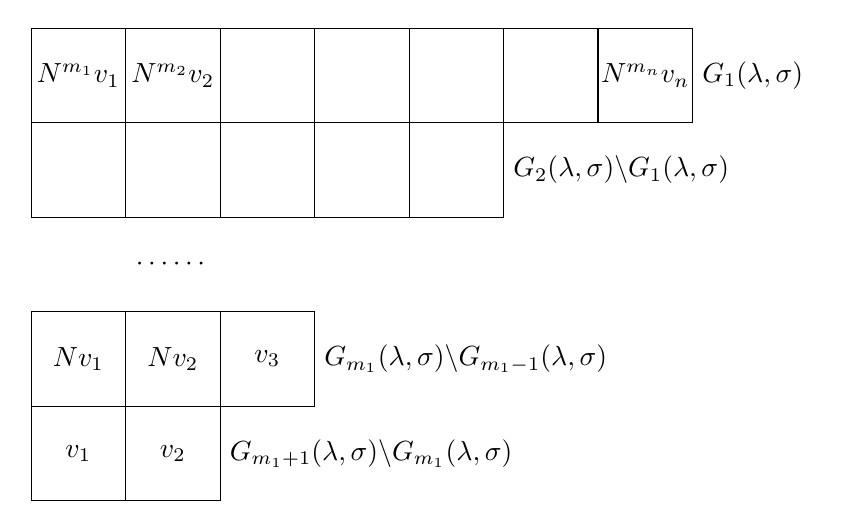
\begin{tikzpicture}[scale=1.2]
                  \foreach[count=\i] \len in {7, 7, 5, 3, 3, 2}
                  \draw (0, -\i+1) -- (\len, -\i+1);

                  \foreach \i in {0, 1, 2}
                  \draw (\i, -3) -- (\i, -5);

                  \draw (3, -3) -- (3, -4);

                  \foreach \i in {0,...,5}
                  \draw (\i, 0) -- (\i, -2);

                  \foreach \i in {6, 7}
                  \draw (\i, 0) -- (\i, -1);

                  \foreach \i in {1, 2} {
                  \node at (\i-.5, -4.5) {$v_{\i}$};
                  \node at (\i-.5, -.5) {$N^{m_{\i}}v_{\i}$};
                  }
                  \foreach \i in {1, 2}
                  \node at (\i-.5, -3.5) {$Nv_{\i}$};

                  \node at (3-.5, -3.5) {$v_{3}$};
                  \node at (6.5, -.5) {$N^{m_n}v_n$};
                  \node at (1.5, -2.5) {$\cdots\cdots$};

                  \node[anchor=west] at (7, -.5) {$G_1(\lambda,\sigma)$};
                  \node[anchor=west] at (5, -1.5) {$G_2(\lambda,\sigma) \backslash G_1(\lambda,\sigma)$};
                  \node[anchor=west] at (3, -3.5) {$G_{m_1}(\lambda,\sigma) \backslash G_{m_1-1}(\lambda,\sigma)$};
                  \node[anchor=west] at (2, -4.5) {$G_{m_1+1}(\lambda,\sigma) \backslash G_{m_1}(\lambda,\sigma)$};
              \end{tikzpicture}
              \caption{将若当基排列成Young图形式}
              \label{fig:17:若当基Young图形式}
          \end{figure}

    \item 接下来要确定每个若当循环基的长度,也就是Young图每一列的长度,我们应当从行的性质入手,因为这是我们目前仅有的可以计算的信息. 我们需要求解每个$G_j(\lambda,\sigma)$及其维数(目前只有维数有用,但后续求解具体若当基时其中的向量也是有用的),直到某个$G_j(\lambda,\sigma)$的维数等于$G_\lambda$的维数,因为Young图中所有方格与$G_\lambda$的一组基一一对应,因此方格总数就等于$G_\lambda$的维数. 另一方面由\autoref{thm:广义特征性质},$N$是$G_\lambda$上的幂零线性变换,且在其它广义特征子空间上是双射,因此在核空间最高次数也只能是$G_\lambda$的维数.

          在求出各个$G_j(\lambda,\sigma)$的维数后阶梯形状也即确定,因为各层向量个数确定了. 举个简单的例子,假设$G_\lambda$是11维空间,满足$G_1(\lambda,\sigma)$,$G_2(\lambda,\sigma)$,$G_3(\lambda,\sigma)$的维数分别为5,9,11. 对照Young图每行右侧的标注,这说明从最上方一行往下的向量个数依次为5,4($=9-5$),2($=11-9$),具体Young图为
          \begin{figure}[H]
              \centering
              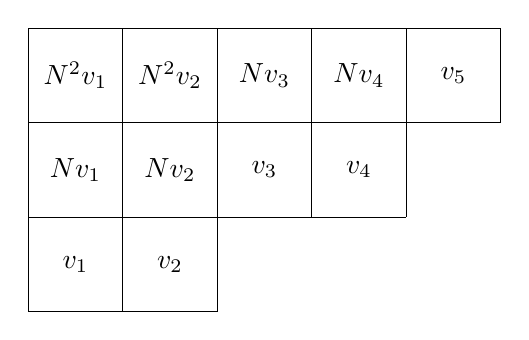
\begin{tikzpicture}[scale=1.2]
                  \foreach[count=\i] \len in {5, 5, 4, 2}
                  \draw (0, -\i+1) -- (\len, -\i+1);

                  \foreach \i in {0,...,5}
                  \draw (\i, 0) -- (\i, -1);
                  \foreach \i in {0,...,4}
                  \draw (\i, -1) -- (\i, -2);
                  \foreach \i in {0, 1, 2}
                  \draw (\i, -2) -- (\i, -3);

                  \node at (.5, -.5) {$N^2v_1$};
                  \node at (1.5, -.5) {$N^2v_2$};
                  \node at (2.5, -.5) {$Nv_3$};
                  \node at (3.5, -.5) {$Nv_4$};
                  \node at (4.5, -.5) {$v_5$};
                  \node at (.5, -1.5) {$Nv_1$};
                  \node at (1.5, -1.5) {$Nv_2$};
                  \node at (2.5, -1.5) {$v_3$};
                  \node at (3.5, -1.5) {$v_4$};
                  \node at (.5, -2.5) {$v_1$};
                  \node at (1.5, -2.5) {$v_2$};
              \end{tikzpicture}
          \end{figure}
          然后我们就能得到每组若当循环基的长度,即每个若当块的阶数,分别为$3,3,2,2,1$.
\end{enumerate}

基于上面的求解过程,我们就可以得到一般性的Young图大小的决定公式如下:
\begin{theorem}{}{Young图行长度}
    令$r_j$表示Young图从上至下第$j$行的格数,则有(其中$N=\sigma-\lambda I$):
    \begin{enumerate}
        \item $r_1=\dim V-r(N)$;
        \item $r_j=r(N)^{j-1}-r(N)^j(j>1)$.
    \end{enumerate}
\end{theorem}
\begin{proof}
    根据\autoref{fig:17:若当基Young图形式} 中每行右侧的标注的含义,第一行的格数就是$G_1(\lambda,\sigma)$的维数,即特征子空间的维数,即$\dim V-r(N)$;第$j(j>1)$行的格数就是$G_j(\lambda,\sigma)$的维数减去$G_{j-1}(\lambda,\sigma)$的维数,由线性映射基本定理,$\dim G_j(\lambda,\sigma)=\dim G_\lambda-r(N)^j$,$\dim G_{j-1}(\lambda,\sigma)=\dim G_\lambda-r(N)^{j-1}$,因此第$j$行的格数就是$r(N)^{j-1}-r(N)^j$.
\end{proof}

基于上述定理,我们可以进一步得到每个特征值对应的若当块个数和每个若当块大小的公式. 进一步地,这些公式实际上就表明了若当标准形的唯一性,因为每个特征值对应的若当块的个数和大小都可以被如下公式唯一确定. 我们将这一定理总结如下:
\begin{theorem}{}{若当标准形唯一}
    设$V$是$n$维复向量空间,$\sigma\in \mathcal{L}(V)$,$\lambda_1,\ldots,\lambda_m$为其互异的特征值,记$N_j=\sigma-\lambda_j I$,则主对角元为$\lambda_j$的若当块的个数$n_j$为
    \begin{equation} \label{eq:17:若当块个数}
        n_j=n-r(N_j),
    \end{equation}
    其中$t$级若当块$J_t(\lambda_j)$的个数$n_j(t)$为
    \begin{equation} \label{eq:17:若当块大小}
        n_j(t)=r(N_j^{t+1})+r(N_j^{t-1})-2r(N_j^t),
    \end{equation}
    以上公式表明,除若当块的排列次序外,一个线性变换对应的若当标准形唯一.
\end{theorem}
\begin{proof}
    实际上,证明这一定理就是要从\autoref{thm:Young图行长度} 中得到的Young图每行的长度推出Young图有多少列,以及每列的长度. 很显然,Young图的列数就是第一行的长度,即$\dim V-r(N_j)$. 进一步观察,我们知道Young图第$j$行与第$j+1$行的长度之差来源于有$r_j-r_{j+1}$(记号来源于\autoref{thm:Young图行长度})组循环若当基长度终止于$j$,因此大小为$j$的若当块的个数就是$r_j-r_{j+1}=r(N_j)^{t+1}+r(N_j)^{t-1}-2r(N_j)^t$.
\end{proof}

尽管我们理论上可以通过上述过程得到任意复向量空间上的线性变换的若当块的个数和大小,但我们知道,直接对线性变换计算特征值是困难的,因此更多的时候我们仍然是利用线性变换和它的矩阵表示的特征值与广义特征向量的对应关系,将求解线性变换的若当标准形转化为求解其某个矩阵表示的若当标准形.

于是我们讨论矩阵的情况. 我们考虑$P^{-1}AP=J$,其中$P$为过渡矩阵,$J$为$A$的若当标准形. 我们可以将$A$视为$\sigma(\alpha)=A\alpha$在自然基下的矩阵,于是$\sigma$在\autoref{cor:若当基存在} 给出的基(记为$B$)下的表示矩阵的求解方式就是$\sigma(B)=(B)J$,将$B$组成的矩阵记作$P$,代入$\sigma$的定义,$\sigma(B)=(B)J$就等同于$AP=PJ$,即$P^{-1}AP=J$,故如果我们要求矩阵相似于其若当标准形的过渡矩阵,问题转化为求解$\sigma(\alpha)=A\alpha$的若当基然后排列成矩阵即可.

然而我们知道,求解$\sigma$的若当基需要求解各个$G_i(\lambda,\sigma)=\ker(\sigma-\lambda I)^i$,代入$\sigma(\alpha)=A\alpha$可知,$G_i(\lambda,\sigma)$实际上就是$(A-\lambda I)^iX=0$的解. 所以对于矩阵而言,上述所有的过程都只是不断对矩阵求幂然后解线性方程组,因此是一定可解的. 我们用解空间替代各个$G_i(\lambda,\sigma)$重复上述过程可以得到如下定理:
\begin{theorem}{}{}
    设$A$是$n$阶复矩阵,$\lambda_1,\ldots,\lambda_m$为其互异的特征值,则主对角元为$\lambda_j$的若当块的个数$n_j$为
    \begin{equation} \label{eq:17:矩阵若当块个数}
        n_j=n-r(A-\lambda_j I),
    \end{equation}
    其中$t$级若当块$J_t(\lambda_j)$的个数$n_j(t)$为
    \begin{equation} \label{eq:17:矩阵若当块大小}
        n_j(t)=r(A-\lambda_j I)^{t+1}+r(A-\lambda_j I)^{t-1}-2r(A-\lambda_j I)^t,
    \end{equation}
    以上公式表明,除若当块的排列次序外,一个矩阵对应的若当标准形唯一.
\end{theorem}

最后我们需要提到一点,根据上面的叙述,若当标准形在不考虑若当块的排列顺序的情况下是唯一的. 因此任一复数域上矩阵均有唯一的若当标准形(相似标准形),因此我们可以知道,两矩阵相似的一个充要条件是两矩阵有相同的若当标准形(不考虑若当块的排列顺序),这也是判定两个矩阵是否相似的关键,当然之后我们还会学到其它判定方式,届时我们再做总结.

接下来我们将讨论如何求出Young图中所有方格中的向量,当然实际上只需确定每个终止向量即可得到所有向量. 在正式讨论之前,我们先考虑一种投机取巧的方式. 事实上,如果题目只要求我们求解矩阵的若当标准形时,如果我们要求解过渡矩阵,也有简单的方法. 要求$P$使得$P^{-1}AP=J$,则有$AP=PJ$. 假定$P$为$n$阶矩阵,我们可以设$P=(X_1,\ldots,X_n)$,剩下的任务就是解方程了. 因此这种方法非常简单,缺陷在于绕开了若当基这一本质的问题.
\begin{example}{}{}
    利用上述方法求解矩阵\[\begin{pmatrix}
            2 & 3 & 2 \\ 1 & 8 & 2 \\ -2 & -14 & -3
        \end{pmatrix}\]的若当标准形以及对应的过渡矩阵.
\end{example}

\begin{solution}

\end{solution}

下面我们将讨论对于一般的线性变换,无法投机取巧时,或者希望从更本质的角度求解时,我们应当使用的方法.

\begin{center}
    \textbf{\heiti 第二步\quad 求解 $\boldsymbol{v_1,\ldots,v_n}$}
\end{center}

\begin{enumerate}
    \item 实际上,我们在前述求解若当块大小的过程中求出了各个$G_j(\lambda,\sigma)$,接下来我们需要利用这些向量将之前确定形状的阶梯内容填满. 我们首先将阶梯最上方的向量确定,实际上就是利用求出的$G_{m_1+1}(\lambda,\sigma)$(也就是$V$)和$G_{m_1}(\lambda,\sigma)$求出二者之差. 似乎很简单,但若仔细思索便会发现线性空间的差并不一定好求. 举一个简单的例子,设$G_{m_1+1}(\lambda,\sigma)=\{\alpha_1,\alpha_2,\alpha_3,\alpha_4\}$,$G_{m_1}(\lambda,\sigma)=\{\beta_1,\beta_2\}$. 这其中出现的所有向量可能都完全不一样,所以作差并不容易. 但我们有一种好方法,如果我们每次从$G_{m_1+1}(\lambda,\sigma)$中挑选两个向量和$G_{m_1}(\lambda,\sigma)$中的两个向量放在一起,如果这四个向量线性无关,这就说明这两个挑出的向量就是作差的结果. 原因在于这相当于$G_{m_1}(\lambda,\sigma)$直和这两个向量长成的空间后得到了$G_{m_1+1}(\lambda,\sigma)$. 如果四个向量线性相关,这说明挑选的向量有在$G_{m_1}(\lambda,\sigma)$中的.

    \item 接下来继续计算第二行中的向量. 实际上算出第一行后第二行中部分向量就已经确定了,例如图上的$Nv_1$和$Nv_2$. 我们这时用类似的方法求解$G_{m_1}(\lambda,\sigma)$和$G_{m_1-1}(\lambda,\sigma)$的差,如图只需要确定一个向量,但这一个向量的确定除了要像(a)中一样每次从$G_{m_1}(\lambda,\sigma)$中选择一个与$G_{m_1-1}(\lambda,\sigma)$的基一起判断线性相关性外,还需要确保这个向量和已经求出的$Nv_1$和$Nv_2$是线性无关的,因为它们构成$G_{m_1}(\lambda,\sigma)$的一组基.

          总结一下,处于$G_j(\lambda,\sigma)\backslash G_{j-1}(\lambda,\sigma)$对应的行的需要补充的向量$v$应当满足如下三个条件:
          \begin{enumerate}
              \item $v\in G_j(\lambda,\sigma)$;

              \item $v\notin G_{j-1}(\lambda,\sigma)$(通过加入$G_{j-1}(\lambda,\sigma)$)的基保证线性无关判断);

              \item $v$与同一行中左边已求出的向量线性无关.
          \end{enumerate}

    \item 最后,我们将所有求出的基按照若当基原先的排列顺序重新组合即可. 如果求矩阵相似于若当标准形的过渡矩阵,则按顺序按列摆放即可.
\end{enumerate}

我们可以通过一个例子来说明上述过程.
\begin{example}{}{}
    设$V$是由两个变量$x,y$生成的次数不大于2的多项式函数(例如$xy^2$不是,因为次数等于1+2=3,$x^2+y$是)关于一般的多项式加法和数乘构成的线性空间,于是我们可以取一组基为$\{1,x,y,x^2,y^2,xy\}$,定义$\sigma\in \mathcal{L}(V)$为
    \[\sigma(f(x,y))=\dfrac{\partial}{\partial x}f(x,y).\]
    求$V$的一组基使得$\sigma$在这组基下的矩阵是若当标准形.
\end{example}
\begin{solution}

\end{solution}

\section{若当标准形的应用}
\subsection{求解不变子空间}
在不变子空间一节中我们提到,我们可以利用若当标准形求解不变子空间. 下面是一个与若当块直接相关的例子:
\begin{example}{}{}
    设$V$为$n$维复向量空间,$\sigma\in \mathcal{L}(V)$,$\sigma$在基$v_1,\ldots,v_n$下的矩阵是一个若当块
    \[\begin{pmatrix}
            \lambda & 1       & 0      & \cdots & 0       \\
            0       & \lambda & 1      & \cdots & 0       \\
            \vdots  & \vdots  & \vdots & \ddots & \vdots  \\
            0       & 0       & 0      & \cdots & \lambda
        \end{pmatrix},\]
    证明:
    \begin{enumerate}
        \item $V$中包含$v_n$的不变子空间只有$V$自身;

        \item $V$中任意非零不变子空间都包含$v_1$;

        \item $V$不能分解为两个非平凡的不变子空间的直和;

        \item $V$中有且仅有$n+1$个不变子空间,它们分别是
              \[\{0\},\spa(v_1),\spa(v_1,v_2),\ldots,\spa(v_1,\ldots,v_{n-1},v_n)\]
    \end{enumerate}
\end{example}

\begin{solution}
    \begin{enumerate}
        \item 设$W$是包含$v_n$的不变子空间,根据线性映射矩阵表示的定义,$\sigma(v_n)=\lambda v_n+v_{n-1}\in W$,故$v_{n-1}\in W$,同理可得$v_{n-2},\ldots,v_1\in W$,即$W=V$.

        \item 设$U$为任一非零不变子空间,那么$U$中存在一个非零向量$v$,则$v$一定可以表达为
              \[v=k_1v_1+\cdots+k_sv_s(s\leqslant n),\]
              其中$k_s\neq 0$. 由$\sigma(v)\in U$以及线性映射矩阵表示有
              \begin{align*}
                  \sigma(v) & = \lambda k_1v_1+k_2(\lambda v_2+v_1)+\cdots+k_s(\lambda v_s+v_{s-1}) \\
                            & = \lambda v+k_2v_1+\cdots+k_sv_{s-1}\in U,
              \end{align*}
              因此$k_2v_1+\cdots+k_sv_{s-1}\in U$,同理进一步作用$\sigma$有$k_3v_1+\cdots+k_sv_{s-2}\in U$,以此类推有$k_sv_1\in U$. 又$k_s\neq 0$,故$v_1\in U$,命题得证.

        \item 利用上一点显然.

        \item 显然$\{0\},\spa(v_1),\spa(v_1,v_2),\ldots,\spa(v_1,\ldots,v_{n-1},v_n)$都是不变子空间,下面证明不变子空间一定在它们当中.

              设$U$为任一不变子空间,若$U=\{0\}$,则也符合结论. 我们考虑非零的情况,设$\beta_1,\ldots,\beta_s$是$U$的一组基,并且假设
              \[\beta_i=a_{i1}v_1+a_{i2}v_2+\cdots+a_{it}v_t,\enspace i=1,2,\ldots,s\]
              其中满足至少有一个$i$使得$a_{it}\neq 0$(把所有基下表示末尾的0去除即可). 对于满足$a_{it}\neq 0$的$i$,由于$U$是不变子空间,故$\sigma(\beta_i)\in U$,与第二点证明完全相同,我们得到
              \begin{align*}
                  a_{i2}v_1+a_{i3}v_2+\cdots+a_{it}v_{t-1}\in U, \\
                  a_{i3}v_1+a_{i4}v_2+\cdots+a_{it}v_{t-2}\in U, \\
                  \cdots                                         \\
                  a_{i,t-1}v_1+a_{it}v_2\in U,                   \\
                  a_{it}v_1\in U.
              \end{align*}
              由于$a_{it}\neq 0$,故由最后的式子知道$v_1\in U$. 代入倒数第二个式子知道$v_2\in U$,以此类推,最终得到$\spa(v_1,\ldots,v_t)\subset U$,而$U\subset\spa(v_1,\ldots,v_t)$显然(因为每个$\beta_i$都在其中),故命题得证.
    \end{enumerate}
\end{solution}

因此我们如果能将线性变换在一组基下表示为若当块,我们就可以很快地利用这一例子的结论写出其不变子空间. 但我们有时候会遇到线性变换在一组基下表示为多个若当块的情况,这时我们可能需要通过组合不同若当块对应的不变子空间来得到线性变换的不变子空间(很容易知道不相交的不变子空间的直和还是不变子空间,因为矩阵表示还是分块对角矩阵),并且同时还要证明组合出来的就是全部的不变子空间. 下面就是一个非常经典的例子:
\begin{example}{}{}
    设$V$是复数域上的$n$维线性空间,$\sigma\in\mathcal{L}(V)$,若$\sigma$有$n$个不同的特征值$\lambda_1,\ldots,\lambda_n$,求$\sigma$的不变子空间的个数.
\end{example}
\begin{solution}
    显然$\sigma$可对角化,每个对角元素就是一阶若当块,因此我们需要考虑组合这些若当块对应的基构成新的不变子空间. 由可对角化我们有
    \[V=V_{\lambda_1}\oplus\cdots\oplus V_{\lambda_n},\]
    结合$\dim V=n$可知每个特征子空间都是1维的. 根据我们组合的思想,我们知道对于任意的$1\leqslant j_1<j_2<\cdots<j_r\leqslant n$,$r=1,2,\ldots,n$,$V_{\lambda_{j_1}}\oplus\cdots\oplus V_{\lambda_{j_r}}$都是不变子空间. 这样的不变子空间加上零空间的个数总和为$\mathrm{C}_n^0+\mathrm{C}_n^1+\cdots+\mathrm{C}_n^n=2^n$.

    下面我们需要说明这些不变子空间是全部的不变子空间. 设$U$为任一不变子空间,若为零空间则符合要求,若不是零空间,设$\dim U=m>0$,$U$的一组基为$\beta_1,\ldots,\beta_m$,将其扩充为$V$的一组基$\beta_1,\ldots,\beta_m,\beta_{m+1},\ldots,\beta_n$,则在这组基下$\sigma$的矩阵为
    \[B=\begin{pmatrix}
            A & C \\ O & D
        \end{pmatrix},\]
    于是$\sigma\vert_W$的矩阵为$A$,对应特征多项式$|\lambda E-A|$可以整除$\sigma$的特征多项式$|\lambda E-B|=|\lambda E-A||\lambda E-D|$,由于$\sigma$有$n$个不同的特征值,因此$\sigma\vert_W$必定有$m$个不同的特征值$\lambda_{l_1},\ldots,\lambda_{l_m}$,且$1\leqslant l_1<\cdots<l_m\leqslant n$,而对每个特征值$\lambda_{l_i}$都有特征向量$\alpha_i\in W$,满足$\sigma\vert_W(\alpha_i)=\lambda_{l_i}\alpha_i$,因此$\sigma(\alpha)=\lambda_{l_i}\alpha_i$,即$\alpha_i\in V_{\lambda_{l_i}}$,故$V_{\lambda_{l_1}}\oplus\cdots\oplus V_{\lambda_{l_m}}\subset U$. 再结合
    \[\dim(V_{\lambda_{l_1}}\oplus\cdots\oplus V_{\lambda_{l_m}})=m=\dim U,\]
    故$U=V_{\lambda_{l_1}}\oplus\cdots\oplus V_{\lambda_{l_m}}$,故所有不变子空间都是之前讨论的$2^n$种之一,命题得证.
\end{solution}

当然需要注意的是,不变子空间的个数不一定有限,例如对于数乘变换$\sigma=kI\in\mathcal{L}(V)$,很容易验证$V$的任意子空间都是其不变子空间.

\subsection{矩阵求幂与马尔可夫链}

若当标准形的另一个应用在于我们可以利用它计算矩阵的幂,因为若当块的幂的计算是简单的,这一点与对角矩阵是类似的:
\[J_k(a)^n=(aE+J_k(0))^n=a^nE+\mathrm{C}_n^1a^{n-1}J_k(0)+\cdots+\mathrm{C}_n^nJ_k(0)^n\]
同时我们也知道$J_k(0)^k=O$(幂零矩阵),所以利用若当标准形求解矩阵的幂是简单的. 我们来看一个例子:
\begin{example}{}{}
    设$A=\begin{pmatrix}
            2 & 6 & -15 \\ 1 & 1 & -5 \\ 1 & 2 & -6
        \end{pmatrix}$,求$A^{m}(m\geqslant 1)$.
\end{example}
\begin{solution}

\end{solution}

下面是一个非常经典的例子,在接下来的讨论中还会有应用:
\begin{example}{}{若当m次幂}
    设$J=J_n(a)$是特征值为$a$的$n$阶若当块,求$J^m$的若当标准形,其中$m$为非零整数.
\end{example}
\begin{solution}
    我们需要分别考虑$a\neq 0$和$a=0$的情况:
    \begin{enumerate}
        \item 当$a\neq 0$时,首先显然$J^m$的特征值都为$a^m$,我们先处理$m\geqslant 1$的情况,我们有
              \[J^m=(aE+J(0))^m=a^mE+\mathrm{C}_m^1a^{m-1}J_n(0)+\cdots+\mathrm{C}_m^mJ_n(0)^m.\]
              故$r(J^m-a^mE_n)=r(\mathrm{C}_m^1a^{m-1}J_n(0)+\cdots+\mathrm{C}_m^mJ_n(0)^m)=n-1$(很容易通过$J_n(0)$的幂次的特点写出这一矩阵,然后通过行列式秩判断),因此根据\autoref{thm:若当标准形唯一} 可知$J^m$的若当块个数为$n-(n-1)=1$,因此$J^m$的若当标准形就是$J_n(a^m)$.

              然后我们考虑$m=-1$的情况,显然$J^{-1}$的特征值为$a^{-1}$,这里我们借用\autoref{ex:分式求逆1} 的分式思想,得到
              \[J^{-1}=\dfrac{1}{a}E_n-\dfrac{1}{a^2}J_n(0)+\cdots+(-1)^{n-1}\dfrac{1}{a^n}J_n(0)^{n-1}.\]
              故$r(J^{-1}-\dfrac{1}{a}E_n)=r(-\dfrac{1}{a^2}J_n(0)+\cdots+(-1)^{n-1}\dfrac{1}{a^n}J_n(0)^{n-1})=n-1$,因此$J^{-1}$的若当块个数为$n-(n-1)=1$,因此$J^{-1}$的若当标准形就是$J_n(a^{-1})$.

              最后处理$m\leqslant -2$的情况,注意到$J^m=(J_n^{-1})^{-m}$,故根据前面$m\geqslant 1$的讨论,$J^m$的若当标准形就是$J_n((a^{-1})^{-m})=J_n(a^m)$.

              综上所述,无论$m$取什么整数值,$J^m$的若当标准形就是$J_n(a^m)$.

        \item 当$a=0$时,我们有$m\geqslant n$时$J^m=O$,此时若当标准形也就是零矩阵. 我们考虑$m<n$的情况,我们需要使用\autoref{thm:若当标准形唯一} 的结论来辅助我们求解$J^m$的若当标准形,因此我们需要研究$(J^m)^k$的秩. 我们做带余除法,$n=mq+r(0\leqslant r<m)$,则根据$J_n(0)$的幂次的特点,我们有
              \[r((J^m)^k)=n-mk,\enspace 0\leqslant k\leqslant q,\enspace r((J^m)^k)=0,\enspace k\geqslant q+1.\]
              因此
              \begin{enumerate}
                  \item $1\leqslant k<q$时,$J_k(0)$的个数为$r((J^m)^{k-1})+r((J^m)^{k+1})-2r((J^m)^k)=(n-m(k-1))+(n-m(k+1))-2(n-mk)=0$;
                  \item $k=q$时,$J_k(0)$的个数为$r((J^m)^{q-1})+r((J^m)^{q+1})-2r((J^m)^q)=(n-m(q-1))+0-2(n-mq)=m-r$;
                  \item $k=q+1$时,$J_k(0)$的个数为$r((J^m)^q)+r((J^m)^{q+2})-2r((J^m)^{q+1})=(n-mq)+0-0=r$.
                  \item $k>q+1$时,$J_k(0)$的个数为0.
              \end{enumerate}
              综上所述,$J^m$的若当标准形是$\diag(J_q(0),\ldots,J_q(0),J_{q+1}(0),\ldots,J_{q+1}(0))$,其中$J_q(0)$的个数为$m-r$,$J_{q+1}(0)$的个数为$r$.
    \end{enumerate}
\end{solution}

由于复数域上任意矩阵都有若当标准形,因此利用若当标准形,我们可以求出复数域上任意矩阵的任意幂次. 于是我们会有一个问题,即任意给定一个矩阵,当我们取其幂次趋向于无穷时,会得到一个什么样的矩阵呢?是所有元素都有限的矩阵,还是有些元素可能趋于无穷了呢?

\subsection{若当标准形与矩阵分解}
矩阵分解是我们讨论标准形时绕不开的话题,接下来我们讨论若当标准形应用于矩阵分解的情形. 我们首先讨论平方根分解,这一点是之前线性变换平方根讨论的延续. 下面这一结论是相当经典的:
\begin{theorem}{}{若当标准形m次根}
    在复数域上,我们有如下关于若当标准形的根式结论:
    \begin{enumerate}
        \item 设$a\neq 0$,则存在矩阵$A$使得$A^m=J_n(a)$;
        \item 当$n\geqslant 2$时,不存在矩阵$A$使得$A^m=J_n(0)$.
    \end{enumerate}
\end{theorem}

\begin{proof}
    \begin{enumerate}
        \item 根据\autoref{ex:若当m次幂},我们知道$J_n(a)^m\sim J_n(a^m)$. 设$b^m=a$(在复数域上一定存在这样的$b$),则$J_n(b)^m\sim J_n(a)$,因此存在可逆矩阵$P$使得$P^{-1}J_n(b)^mP=J_n(a)$,取$A=P^{-1}J_n(b)P$即可.

        \item 反证法. 若存在矩阵$A$使得$A^m=J_n(0)$,则$A$显然也为$n$阶幂零矩阵,因此有$A^n=O$(因此至少有$m\leqslant n$). 设$n=mq-r(m\geqslant 2,0\leqslant r<m)$,则$O=A^{n+r}=(A^m)^q=J_n(0)^q\neq O$,这是因为$J_n(0)$至少需要$n$次才能化零,但$n=mq-r(m\geqslant 2,0\leqslant r<m)$表明$q<n$,故矛盾.
    \end{enumerate}
\end{proof}

接下来我们考虑之前已经证明的\autoref{thm:幂零平方根} 的\ref*{item:16:幂零平方根:2},即可逆线性变换一定有平方根,我们现在可以使用若当标准形的方式证明. 我们直接使用矩阵证明即可,因为基固定的情况下矩阵和线性映射一一对应. 因为可逆线性变换对应可逆矩阵$A$,可逆矩阵特征值均不为0,因此每个对应的若当标准形$J$的若当块对角线上都不为0,均有平方根(即上述定理中$m=2$,我们记$B^2=J$). 进一步地,由于一定存在可逆矩阵$P$使得$P^{-1}AP=J$,我们取$C=PBP^{-1}$,则$C^2=PB^2P^{-1}=PJP^{-1}=A$,故我们找到了任意可逆矩阵对应的平方根$C$. 这一结论显然可以进一步推广,即任意复数域上的可逆线性变换和可逆矩阵一定有$m$次方根.

利用若当标准形,我们还可以有以下著名的Jordan-Chevalley分解. 这一定理的证明过程将会给出我们利用若当标准形证明一般矩阵性质的通用方法,一般包含如下步骤:
\begin{enumerate}
    \item 证明结论对于若当块成立;
    \item 证明结论对于若当标准形成立;
    \item 利用问题在相似下的不变性证明结论对于一般矩阵成立.
\end{enumerate}

事实上,上面讨论任意复可逆矩阵均有平方根也是遵循这一范式证明的,我们也是先证明了对角线元素非零的若当块一定有平方根,那么自然若当标准形是由若当块构成的分块对角矩阵也满足这一性质,然后利用$(P^{-1}AP)^n=P^{-1}A^nP$这一相似具有的运算特点证明对一般可逆矩阵有平方根成立. 总而言之,当我们希望使用若当标准形证明矩阵具有的性质时,这些性质在相似下要有一定的不变性,然后我们遵照上述范式即可给出证明. 因此,我们发现了研究相似标准形的一个重要的意义,因为这些很简单的矩阵一般而言都是具有很好的性质的,再结合很多性质在相似下都可以保持,因此我们可以通过研究更容易处理的相似标准形来研究一般矩阵的性质. 下面我们就开始证明这一著名的分解:

\begin{theorem}{Jordan-Chevalley分解}{}
    设$A$是$n$阶复矩阵,则$A$可分解为$A=B+C$,其中$B,C$满足如下条件:
    \begin{enumerate}
        \item $B$是可对角化的;
        \item $C$是幂零的;
        \item $BC=CB$;
        \item $B,C$均可以表示为$A$的多项式.
    \end{enumerate}
    不仅如此,满足上述条件1-3的分解是唯一的.
\end{theorem}

\begin{proof}
    我们首先对若当块$J_n(a)$证明这一定理. 事实上这非常显然,我们取$B=aE_n$,$C=J_n(0)$,则$B$可对角化,$C$是幂零的,且$BC=CB=aJ_n(0)$. 又因为$O=C^n=(J_n(a)-B)^n$,因此我们取$f(x)=(x-a)^n+a$,代入$x=J_n(a)$有
    $f(J_n(a))=(J_n(a)-aE_n)^n+aE_n=aE_n=B$,因此$B$表示为了$A$的多项式,而$C=J_n(a)-B=J_n(a)-f(J_n(a))$也是$A$的多项式.

    接下来推广到若当标准形$J$,我们假设$J$互不相同的特征值为$\lambda_1,\ldots,\lambda_m$,设每个特征值$\lambda_i$对应$s_i$个若当块,则可以将$J$表示为
    \[J=\begin{pmatrix}
            J_{11} &        &          &        &        &        &          \\
                   & \ddots &          &        &        &        &          \\
                   &        & J_{1s_1} &        &        &        &          \\
                   &        &          & \ddots &        &        &          \\
                   &        &          &        & J_{m1} &        &          \\
                   &        &          &        &        & \ddots &          \\
                   &        &          &        &        &        & J_{ms_m}
        \end{pmatrix}.\]
    对每个若当块$J_{ij}$,假设若当块大小为$k_{ij}$,我们类似于前面对若当块的讨论取出每个$M_{ij}=\lambda_i E_{k_{ij}}$,$N_{ij}=J_{k_{ij}}(0)$,然后将这些矩阵按$J$的顺序排列成分块对角矩阵即可得到$M$和$N$,则$J=M+N$,$M$可对角化,$N$是幂零的,且$MN=NM$是容易验证的.

    我们设每个特征值$\lambda_i$对应的最大的若当块的阶数为$k_i$,因此$(J_{ij}-\lambda_{ij})^{k_i}=O$. 我们知道$(\lambda-\lambda_1)^{k_1},\ldots,(\lambda-\lambda_m)^{k_m}$是两两互素的多项式,因此由\nameref{thm:中国剩余定理}可知,存在多项式$f(\lambda)$满足
    \[f(\lambda)=g_i(\lambda)(\lambda-\lambda_i)^{k_i}+\lambda_i,\enspace i=1,\ldots,m\]
    故$f(J_{ij})=g_i(J_{ij})(J_{ij}-\lambda_i)^{k_i}+\lambda_iE_{k_{ij}}=\lambda_iE_{k_{ij}}=M_{ij}$,因此$f(J)=M$也成立. 同理$N=J-M=J-f(J)$也是$J$的多项式,因此命题结论对若当标准形都成立.

    接下来考虑一般情形,设$P^{-1}AP=J$,则$A=PJP^{-1}=P(M+N)P^{-1}=PMP^{-1}+PNP^{-1}$. 取$B=PMP^{-1}$,$C=PNP^{-1}$,则$B$可对角化,$C$是幂零的,且$BC=CB$,$B,C$均可以表示为$A$的多项式都可以从$M,N$具有这样的性质立刻得到,即这一问题是在相似下不变的.

    最后证明唯一性. 假设$A$有另一满足1-3的分解$A=B'+C'$,则$B-B'=C'-C$,由$B'C'=C'B'$,结合$A=B'+C'$可知$AB'=B'A,AC'=C'A$,又因为$B=f(A)$,故$BB'=B'B$,同理有$CC'=C'C$. 设$C^r=O,C'^t=O$,用二项式定理可知$(C-C')^{r+t}=O$,因此$(B-B')^{r+t}=O$.

    我们知道$B$和$B'$可对角化且$BB'=B'B$,根据上一讲的习题可知它们可以同时对角化,即存在可逆矩阵$Q$使得$Q^{-1}BQ$和$Q^{-1}B'Q$均为对角矩阵. 注意到
    \[(Q^{-1}BQ-Q^{-1}B'Q)^{r+t}=(Q^{-1}(B-B')Q)^{r+t}=Q^{-1}(B-B')^{r+t}Q=O,\]
    又两对角矩阵的差是对角矩阵,因此只能有$Q^{-1}BQ=Q^{-1}B'Q$,即$B=B'$,从而$C=C'$也成立,因此唯一性得证.
\end{proof}

\subsection{求解微分方程}

取一常系数微分方程如下:
\[\dfrac{\mathrm{d}f_1}{\mathrm{d}x^2}-a\dfrac{\mathrm{d}f_1}{\mathrm{d}x}=bf_1.\]
令$\dfrac{\mathrm{d}f_1}{\mathrm{d}x}=f_2$,则上式可以改写为
\[\begin{cases}
        \dfrac{\mathrm{d}f_1}{\mathrm{d}x}=f_2, \\
        \dfrac{\mathrm{d}f_2}{\mathrm{d}x}=af_2+bf_1.
    \end{cases}\]
我们可以将上述方程写成矩阵形式:
\[\dfrac{\mathrm{d}}{\mathrm{d}x}\begin{pmatrix}
        f_1 \\ f_2
    \end{pmatrix}=\begin{pmatrix}
        0 & 1 \\ b & a
    \end{pmatrix}\begin{pmatrix}
        f_1 \\ f_2
    \end{pmatrix}.\]

类似地,$n$阶常微分方程
\[\dfrac{\mathrm{d}f_1}{\mathrm{d}x^n}-a_{n-1}\dfrac{\mathrm{d}f_1}{\mathrm{d}x^{n-1}}-\cdots-a_1\dfrac{\mathrm{d}f_1}{\mathrm{d}x}=bf_1\]
可以改写为
\[\dfrac{\mathrm{d}}{\mathrm{d}x}\begin{pmatrix}
        f_1 \\ f_2 \\ \vdots \\ f_n
    \end{pmatrix}=\begin{pmatrix}
        0      & 1      & 0      & \cdots & 0       \\
        0      & 0      & 1      & \cdots & 0       \\
        \vdots & \vdots & \vdots & \ddots & \vdots  \\
        0      & 0      & 0      & \cdots & 1       \\
        b      & a_1    & a_2    & \cdots & a_{n-1}
    \end{pmatrix}\begin{pmatrix}
        f_1 \\ f_2 \\ \vdots \\ f_n
    \end{pmatrix}=C\begin{pmatrix}
        f_1 \\ f_2 \\ \vdots \\ f_n
    \end{pmatrix}.\]
若有$P^{-1}CP=J$,令
\[P^{-1}\begin{pmatrix}
        f_1 \\ f_2 \\ \vdots \\ f_n
    \end{pmatrix}=\begin{pmatrix}
        g_1 \\ g_2 \\ \vdots \\ g_n
    \end{pmatrix},\]
于是我们有
\[\dfrac{\mathrm{d}}{\mathrm{d}x}\begin{pmatrix}
        g_1 \\ g_2 \\ \vdots \\ g_n
    \end{pmatrix}=J\begin{pmatrix}
        g_1 \\ g_2 \\ \vdots \\ g_n
    \end{pmatrix}.\]

一个直观的事情是$J$越简单方程越容易解,因此这时若当标准形就能帮助我们解决这一问题.

\subsection{求解线性递推方程}

数列的线性递推方程求解是我们高中就曾经接触过的问题,在行列式的运算技巧中我们也曾提及二阶齐次线性递推方程的求解,不过那种方法显然缺乏普适性. 很自然地,我们希望能寻求某种方法来解决$m$阶线性递推方程,不过在此之前,我们需要明确这其中蕴含的线性性究竟在何处.

让我们先从二阶开始,考虑$a_n = k_1 a_{n - 1} + k_2 a_{n - 2}$,显然其特征方程为$x^2 - k_1 x - k_2 = 0$,考虑无重根($\Delta = k_1 + 4k_2 \neq 0$)的情况,有$\lambda_1 = \dfrac{k_1 + \sqrt{k_1 + 4k_2}}{2}, \lambda_2 = \dfrac{k_1 - \sqrt{k_1 + 4k_2}}{2}$,且通项为$a_n = A \lambda_1^n + B \lambda_2^n$,其中$A, B$为待定常数. 而事实上,这个递推方程可以用一个线性映射去表示. 设$T \in \mathcal{L}(\mathbf{F}^2)$为$T(x_1, x_2) = (x_2, k_2 x_1 + k_1 x_2)$,则有$T(a_{n - 2}, a_{n - 1}) = (a_{n - 1}, a_n)$,便可以得到$T^n(a_0, a_1) = (a_n, a_{n + 1})$,也就是说,如果对初值进行$n$次线性变换,我们便可以得到第$n$项的值,但这个计算量过于庞大了. 而回忆我们先前处理算子的幂的方法,很快便能回想起相似标准型,所以接下来我们需要转向求出这一算子的特征值与特征向量.

考虑$T(x_1, x_2) = \lambda (x_1, x_2)$,得到方程组$\begin{cases} x_2 = \lambda x_1 \\ k_2 x_1 + k_1 x_2 = \lambda x_2 \end{cases}.$ 考虑到特征向量不为零向量,所以消去$x_1, x_2$后可以得到关于$\lambda$的方程$\lambda^2 - k_1 \lambda - k_2 = 0$,所以这个方程才会被称为特征方程,因为它的根是算子的特征值. 在没有重根的情况下,解得两个特征值为$\lambda_1, \lambda_2$,而对应的特征向量为$v_1 = (1, \lambda_1), v_2 = (1, \lambda_2)$. 我们知道对应不同特征值的特征向量是线性无关的,并且这里的数量正好等于空间维数,所以这两个特征向量构成了空间的一组基,且算子在这组基下的矩阵表示是简单的,为对角阵$\Lambda = \begin{pmatrix} \lambda_1 & 0 \\ 0 & \lambda_2 \end{pmatrix}$. 设$(a_0, a_1) = c_1 v_1 + c_2 v_2$,而使用矩阵求出坐标再代入基是计算量较小的,所以有 $\Lambda^n \begin{pmatrix}
        c_1 \\ c_2
    \end{pmatrix} = \begin{pmatrix}
        c_1 \lambda_1^n \\ c_2 \lambda_2^n
    \end{pmatrix}$,这便是$(a_n, a_{n + 1})$在这组基下的坐标,代入$v_1, v_2$即可得到通解$a_n = c_1 \lambda_1^n + c_2 \lambda_2^n$.

而对于$m$阶线性递推方程$a_n = k_1 a_{n - 1} + k_2 a_{n - 2} + \cdots + k_m a_{n - m}$,其无重根的情况是二阶的简单推广. 考虑$T \in \mathcal{L}(F^m)$,$T(x_1, x_2, \ldots, x_m) = (x_2, x_3, \ldots, k_m x_1 + k_{m - 1} x_2 + \cdots + k_1 x_m)$,则$T(a_{n - m}, a_{n - m + 1}, \ldots, a_{n - 1}) = (a_{n - m + 1}, a_{n - m + 2}, \ldots, a_n)$,对应的特征方程为$x^m - k_1 x^{m - 1} - \cdots - k_m = 0$,得到特征值为$\lambda_1, \lambda_2, \ldots, \lambda_m$,而对应的特征向量为$v_i = (1, \lambda_i, \lambda_i^2, \ldots, \lambda_i^{m - 1})$,通解为$a_n = \sum_{i = 1}^m c_i \lambda_i^n$. 另一个有趣的事实是所有的特征向量也能组成一个 Vandermonde 矩阵,这也可以从另一个侧面印证为什么要求没有重根.

那么如果存在重根又会发生什么情况呢?我们依然先以一个二阶线性递推方程为例,考虑$a_n = 2 \lambda_0 a_{n - 1} - \lambda_0^2 a_{n - 2}$,构造相应的算子$T(x_1, x_2) = (x_2, 2 \lambda_0 x_2 - \lambda_0^2 x_1)$,则$T(a_{n - 2}, a_{n - 1}) = (a_{n - 1}, a_n)$,特征值易求得为$\lambda_0$,对应特征向量为$(1, \lambda_0)$. 特征空间为一维的,显然不能够对角化,所以它应该对应为二阶的若当块的情况,已知$v_1 = (1, \lambda_0)$,求出满足$(T - \lambda_0 I)v_2 = v_1$的$v_2$即求出了若当基. 满足条件的一个$v_2 = (0, 1)$,在这组基下$T$的矩阵表示为$\begin{pmatrix} \lambda_0 & 1 \\ 0 & \lambda_0 \end{pmatrix} = \lambda_0 I + J$,其中$J = \begin{pmatrix} 0 & 1 \\ 0 & 0 \end{pmatrix}$ 且 $J^2 = O$. 设$(a_0, a_1) = c_1v_1 + c_2v_2$,那么有
\begin{align*}
    M^n \begin{pmatrix} c_1 \\ c_2 \end{pmatrix}
     & = (\lambda_0 I + J)^n \begin{pmatrix} c_1 \\ c_2 \end{pmatrix}                                                          \\
     & = (\lambda^n I + n \lambda^{n - 1} J) \begin{pmatrix} c_1 \\ c_2 \end{pmatrix}                                          \\
     & = \begin{pmatrix} \lambda^n & n \lambda^{n - 1} \\ 0 & \lambda^n \end{pmatrix} \begin{pmatrix} c_1 \\ c_2 \end{pmatrix} \\
     & = \begin{pmatrix} c_1 \lambda^n + n c_2 \lambda^{n - 1} \\ d \lambda^n \end{pmatrix}.
\end{align*}
从而代入$v_1, v_2$有$a_n = c_1 \lambda_0^n + n c_2 \lambda_0^{n - 1}$.

进而我们可以考虑一个$m$阶线性递推方程,且其特征方程有$m$重根$\lambda_0 \neq 0$的情况(特征值为$0$是退化的),这时对应的是一个$m$阶的若当块,重点在于求出其对应的若当基. 首先对应的算子$T$的形式应当为$T(x_1, x_2, \ldots, x_m) = (x_2, x_3, \ldots, (-1)^{m + 1} \binom{m}{0} \lambda_0^m x_1 + (-1)^m \binom{m}{1} \lambda_0^{m - 1} x_2 + \cdots + (-1)^2 \binom{m}{m - 1} \lambda_0 x_{m})$,要求出特征向量即求出满足$(T - \lambda_0 I)v_1 = 0$的$v_1$,这一线性方程组的系数矩阵如下:
\[
    \begin{pmatrix}
        -\lambda_0                            & 1                                     & 0                                           & \cdots & 0                                       \\
        0                                     & -\lambda_0                            & 1                                           & \cdots & 0                                       \\
        \vdots                                & \vdots                                & \vdots                                      & \ddots & \vdots                                  \\
        0                                     & 0                                     & 0                                           & \cdots & 1                                       \\
        (-1)^{m + 1} \binom{m}{0} \lambda_0^m & (-1)^m \binom{m}{1} \lambda_0^{m - 1} & (-1)^{m - 1} \binom{m}{2} \lambda_0^{m - 2} & \cdots & ((-1)^2 \binom{m}{m - 1} - 1) \lambda_0
    \end{pmatrix}
\]
我们能轻松得到$v_1 = (\lambda_0^0, \lambda_0, \lambda_0^2, \ldots, \lambda_0^{m - 1})$是满足前$m-1$行的,代入验证也满足第$m$行. 因为前$m-1$行是线性无关的,所以我们基本上可以宣称第$m$行是前$m-1$行的线性组合,也就是说这个矩阵的秩为$m-1$. 但是,这个线性组合的系数在后续求解若当基的过程中相当重要,所以我们还是要求出来. 记以上系数矩阵为$\begin{pmatrix}
        \beta_1 \\ \beta_2 \\ \vdots \\ \beta_m
    \end{pmatrix}$,$\beta_i$均是行向量. 这个系数求解的关键在于第$2$到第$m-1$个坐标都是有两个行向量来控制的,并且$\beta_m$每个是以组合数为基础的,我们能够很自然的联想到杨辉三角. 首先第$1$个坐标能够给出第一个系数$t_1 = (-1)^m \binom{m - 1}{0} \lambda_0^{m - 1}$,然后第$2$个坐标结合杨辉三角便可以得到$t_2 = (-1)^{m - 1} \binom{m - 1}{1} \lambda_0^{m - 2}$,以此类推,直到第$m-1$个坐标$t_{i - 1} = (-1)^2 \binom{m-1}{m-2} \lambda_0$. 第$m$个坐标我们需要验证其正确性,因为其减去了$1$所以形式上有所区别,但我们可以将其改写为$((-1)^2 \binom{m}{m - 1} - \binom{m - 1}{m - 1}) \lambda_0 = ((-1)^2 \binom{m - 1}{m - 2}) \lambda_0$,与$t_{i-1}$一致. 所以我们有 \[
    \beta_m = t_1 \beta_1 + t_2 \beta_2 + \cdots + t_{m - 1} \beta_{m - 1}.
\]
其中$t_i = (-1)^{m + 1 - i} \binom{m - 1}{i - 1} \lambda_0^{m - i}$.

因为$v_1$的求解是基于齐次线性方程组,所以系数的作用不是很明确. 但当我们开始求解$v_2, v_3, \ldots, v_m$时,这就意味着我们需要处理非齐次线性方程组,需要验证$v_1, v_2, \ldots, v_{m-1}$的第$m$个坐标能根据前$m-1$个坐标由系数$t_i$组合得到. 以$v_2$为例,我们需要验证$\lambda_0^{m-1} = \sum_{i = 1}^{m-1} t_i \lambda_0^{i-1} = \sum_{i = 1}^{m-1} (-1)^{m + 1 - i} \binom{m - 1}{i - 1} \lambda_0^{m - 1}$. 我们可以将其化简为 \begin{align*}
    \sum_{i = 1}^{m-1} (-1)^{m + 1 - i} \binom{m - 1}{i - 1} & = 1  \\
    \sum_{i = 0}^{m-1} \binom{m-1}{i} (-1)^{m - i}           & = 0.
\end{align*}
这是二项式定理的一个特殊情况,所以这个等式是成立的. 根据前$m-1$行,我们可以得到$v_2 = (0, 1, 2 \lambda_0, 3 \lambda_0^2, \ldots, (m - 1) \lambda_0^{m - 2})$. 以此类推,仅依据前$m-1$行的计算,我们可以得到$v_j = (0, 0, \ldots, \binom{j - 1}{j - 1} \lambda_0^0, \binom{j}{j - 1} \lambda_0^1, \ldots, \binom{m - 1}{j - 1} \lambda_0^{m - j})$,且第$1$个非零坐标为第$j$个. 接下来便需要验证$v_j, 1 \leqslant j \leqslant m - 1$的第$m$个坐标能由前$m-1$个坐标线性组合得到,即 \[
    \binom{m - 1}{j - 1} \lambda_0^{m - j} = \sum_{i = 1}^{m - 1} t_i \binom{i - 1}{j - 1} \lambda_0^{i - 1}.
\]
代入后化简得到需要证明的组合恒等式 \[
    \sum_{i = j}^m (-1)^{m + 1 - i} \binom{m - 1}{i - 1} \binom{i - 1}{j - 1} = 0.
\]

\begin{proof}
    注意到 \begin{align*}
        \binom{m - 1}{i - 1} \binom{i - 1}{j - 1} & = \dfrac{(m - 1)!}{(i - 1)! (m - i)!} \dfrac{(i - 1)!}{(j - 1)! (i - j)!} \\ & = \dfrac{(m - 1)!}{(j - 1)! (m - j)!} \dfrac{(m - j)!}{(i - j)! (m - i)!} \\ & = \binom{m - 1}{j - 1} \binom{m - j}{i - j},
    \end{align*}
    所以 \begin{align*}
        \sum_{i = j}^m (-1)^{m + 1 - i} \binom{m - 1}{i - 1} \binom{i - 1}{j - 1}
         & = \sum_{i = j}^m (-1)^{m + 1 - i} \binom{m - 1}{j - 1} \binom{m - j}{i - j}  \\
         & = \binom{m - 1}{j - 1} \sum_{t = 0}^k (-1)^(k + i - t  + 1 - i) \binom{k}{t} \\
         & = \binom{m - 1}{j - 1} \sum_{t = 0}^k \binom{k}{t} (-1)^{k + 1 - t}          \\
         & = \binom{m - 1}{j - 1} (-1) (1 - 1)^k = 0.
    \end{align*}
    其中 $t = i - j, k = m - j$.
\end{proof}

由上可知$v_j$的求解是正确的,这样我们便得到了对应的若当基,$T$在这组基下的表示矩阵为$\lambda_0 I + J$. 设初值在若当基下的表示系数为$c_1, c_2, \ldots, c_m$,则有
\begin{align*}
    M^n \begin{pmatrix}
            c_1 \\ c_2 \\ \vdots \\ c_m
        \end{pmatrix}
     & = (\lambda_0 I + J)^n
    \begin{pmatrix}
        c_1 \\ c_2 \\ \vdots \\ c_m
    \end{pmatrix}                                                                               \\
     & = (\lambda_0^n I + n \lambda_0^{n - 1} J + \cdots + \binom{n}{m - 1} \lambda_0^{n - m + 1} J^{m - 1})
    \begin{pmatrix}
        c_1 \\ c_2 \\ \vdots \\ c_m
    \end{pmatrix}                                                                               \\
     & = \begin{pmatrix}
             \lambda_0^n & n \lambda_0^{n - 1} & \cdots & \binom{n}{m - 1} \lambda_0^{n - m + 1} \\
             0           & \lambda_0^n         & \cdots & \binom{n}{m - 2} \lambda_0^{n - m + 2} \\
             \vdots      & \vdots              & \ddots & \vdots                                 \\
             0           & 0                   & \cdots & \lambda_0^n
         \end{pmatrix}
    \begin{pmatrix}
        c_1 \\ c_2 \\ \vdots \\ c_m
    \end{pmatrix}                                                                               \\
     & = \begin{pmatrix}
             c_1 \lambda_0^n + n c_2 \lambda_0^{n - 1} + \cdots + \binom{n}{m - 1} c_m \lambda_0^{n - m + 1} \\
             c_2 \lambda_0^n + n c_3 \lambda_0^{n - 1} + \cdots + \binom{n}{m - 2} c_m \lambda_0^{n - m + 2} \\
             \vdots                                                                                          \\
             c_m \lambda_0^n
         \end{pmatrix}.
\end{align*}

代入$\{v_j\}$即可得到通解
\[
    a_n = \sum_{i = 1}^m c_i \binom{n}{i - 1} \lambda_0^{n - i + 1}.
\]

而对于一般的若当标准型来说,只需要求出相应的基,然后利用分块对角矩阵的幂次运算即可得到坐标,代入基即可求得通解. 不过需要注意的是,对于$m$阶若当标准型下$n$阶的若当块,其对应的若当基是我们在$m$重根中讨论的前$n$个向量,即
\begin{align*}
    v_1 & = (1, \lambda_0, \lambda_0^2, \ldots, \lambda_0^{m - 1}), \\ v_2 & = (0, 1, 2 \lambda_0, \ldots, (n - 1) \lambda_0^{m - 2}), \\ & \ldots \\ v_n & = (0, 0, \ldots, \binom{n - 1}{n - 1} \lambda_0^0, \binom{n}{n - 1} \lambda_0^1, \ldots, \binom{m - 1}{n - 1} \lambda_0^{m - n}),
\end{align*}
而非前$n$个坐标.

下面给出一道例题,请读者自行尝试.

\begin{example}{}{}
    求解线性递推方程$a_n = 5a_{n - 1} - 8a_{n - 2} + 4a_{n - 3}$,其中$a_0 = 2, a_1 = 4, a_2 = 9$.
\end{example}

\section{实数域上的若当标准形} \label{sec:实数域上的若当标准形}

\begin{theorem}{}{相似域不变性}
    设$A,B$为域$\mathbf{F}$上的同阶方阵,域$\mathbf{K}$是域$\mathbf{F}$的一个扩域,则$A,B$在域$\mathbf{K}$上相似当且仅当它们在域$\mathbf{F}$上也相似.
\end{theorem}
\begin{proof}

\end{proof}

\begin{theorem}{}{实数域上的若当标准形}
    设$A$是$n$阶实矩阵,则$A$在实数域上相似于如下分块对角矩阵:
    \begin{enumerate}
        \item $J=\diag(J_{r_1}(\lambda_1),\ldots,J_{r_k}(\lambda_k),J_{s_1}(a_1,b_1),J_{s_l}(a_l,b_l))$;
        \item $\tilde{J}=\diag(J_{r_1}(\lambda_1),\ldots,J_{r_k}(\lambda_k),\tilde{J}_{s_1}(a_1,b_1),\tilde{J}_{s_l}(a_l,b_l))$
    \end{enumerate}
    其中$\lambda_1,\ldots,\lambda_k,a_1,b_1,\ldots,a_l,b_l$都是实数,$b_1,\ldots,b_l$都非零,$J_{r_i}(\lambda_i)$表示以$\lambda_i$为特征值的通常意义下的若当块,$R_j=\begin{pmatrix}
            a_j & b_j \\ -b_j & a_j
        \end{pmatrix},C_2=\begin{pmatrix}
            0 & 0 \\ 1 & 0
        \end{pmatrix}$,
    \[J_{s_i}(a_i,b_i)=\begin{pmatrix}
            R_i & I_2 &        &        &     \\
                & R_i & I_2    &        &     \\
                &     & \ddots & \ddots &     \\
                &     &        & R_i    & I_2 \\
                &     &        &        & R_i
        \end{pmatrix},\enspace \tilde{J}_{s_i}(a_i,b_i)=\begin{pmatrix}
            R_i & C_2 &        &        &     \\
                & R_i & C_2    &        &     \\
                &     & \ddots & \ddots &     \\
                &     &        & R_i    & C_2 \\
                &     &        &        & R_i
        \end{pmatrix}.\]
\end{theorem}
\begin{proof}

\end{proof}

\begin{summary}

\end{summary}

\begin{exercise}
    % \exquote[]{}

    \begin{exgroup}
        \item
    \end{exgroup}

    \begin{exgroup}
        \item 求矩阵\[\begin{pmatrix}
                2 & 3 & 0  & -1 & 2 & -2 \\ -1 & 0 & 2 & 1 & -1 & -2 \\
                1 & 3 & 2  & 0  & 1 & -4 \\ 5 & 6 & -1 & -2 & 5 & -3 \\
                3 & 3 & -1 & -2 & 3 & -1 \\ 1 & 3 & 2 & 0 & 1 & -4
            \end{pmatrix}\]的若当标准形以及相应的过渡矩阵(提示:这一矩阵是幂零指数为3的幂零矩阵).

        \item 设$A=\begin{pmatrix}
                2 & 1 & 1 \\ -2 & -1 & -2 \\ 1 & 1 & 2
            \end{pmatrix}$,求$A$的若当标准形$J$和矩阵$P$,使得$P^{-1}AP=J$.

        \item 定义$\sigma\in \mathcal{L}(\mathbf{C}^3)$为$\sigma(z_1,z_2,z_3)=(z_2,z_3,0)$. 证明不存在$\tau\in \mathcal{L}(\mathbf{C}^3)$使得$\tau^2=\sigma$.

        \item 证明:存在复数域上的对称矩阵$B,C$,使得$A=BC$,并且可以指定$B,C$中任意一个可逆.

        \item 斐波那契序列(Fibonacci sequence)$\{F_n\}$满足如下定义:
        \[
            F_0 = 0, F_1 = 1, F_n = F_{n - 2} + F_{n - 1}, n \geqslant 2.
        \]
        定义$T \in \mathcal{L}(\mathbf{R}^2)$为$T(x_1, x_2) = (x_2, x_1 + x_2)$.
        \begin{enumerate}
            \item 证明:对于任意非负整数$n$,$T^n(0, 1) = (F_n, F_{n + 1})$.
            \item 求$T$的特征值和对应的特征向量.
            \item 求$F_n$的通项公式.
            \item 证明:对于任意非负整数$n$,$F_n$是最接近$\dfrac{\varphi^n}{\sqrt{5}}$的整数,其中$\varphi = \dfrac{1 + \sqrt{5}}{2}$.
        \end{enumerate}
    \end{exgroup}

    \begin{exgroup}
        \item
    \end{exgroup}
\end{exercise}

\phantomsection
\section*{19 多项式的进一步讨论}
\addcontentsline{toc}{section}{19 多项式的进一步讨论}

\vspace{2ex}

\centerline{\heiti A组}
\begin{enumerate}
    \item
\end{enumerate}

\centerline{\heiti B组}
\begin{enumerate}
    \item
\end{enumerate}

\centerline{\heiti C组}
\begin{enumerate}
    \item
\end{enumerate}

\clearpage

\chapter{有理标准形}

% 相抵、相似、相合的全系不变量
最后我们再来总结一个题型. 一些题目可能需要判断矩阵是否相似,实际上我们有如下基本方法:
\begin{enumerate}
    \item 定义法:找到$P$使得$P^{-1}AP=B$即可,这一般是$A,B$没给出具体矩阵的做法,例如上面的性质证明;

    \item 我们也可以先计算两者特征多项式是否相等(即特征值是否一致),若不一致则一定不相似,得到结论,若一致且均为实对称矩阵则相似,否则不一定相似(因为这是相似的必要条件). 对于这种特征值一致的情况,我们进行对角化,情况如下:
          \begin{enumerate}
              \item 若两矩阵均可对角化,则两矩阵相似:因为特征多项式相等则特征值相等,均可对角化那么对角矩阵也完全一致,因此二者与同一个对角矩阵相似,根据相似这一等价关系的传递性可知两矩阵相似;

              \item 若一个矩阵可对角化,另一个矩阵不可对角化,则一定不相似;

              \item 若两个矩阵都不可对角化,不一定相似. 需要两矩阵各个特征值的几何重数(即各个特征子空间维数)都一致才相似,否则不相似. 这是因为只有几何重数一致才有相同的若当标准形.
          \end{enumerate}
\end{enumerate}

\begin{example}
    设$A,B\in \mathbf{M}_n(\mathbf{F})$,证明:若$A$可逆,则$AB\sim BA$.
\end{example}

\begin{proof}

\end{proof}

\begin{example}
    设$A=\begin{pmatrix}
            0 & 0 & 1 \\ 0 & 1 & 0 \\ 1 & 0 & 0
        \end{pmatrix},B=\begin{pmatrix}
            -1 & 0 & 0 \\ 0 & 0 & 1 \\ 0 & -1 & 2
        \end{pmatrix}$,判断$A$与$B$是否相似.
\end{example}

\begin{solution}

\end{solution}

\vspace{2ex}
\centerline{\heiti \Large 内容总结}

\vspace{2ex}
\centerline{\heiti \Large 习题}

\vspace{2ex}
{\kaishu }
\begin{flushright}
    \kaishu

\end{flushright}

\centerline{\heiti A组}
\begin{enumerate}
    \item
\end{enumerate}

\centerline{\heiti B组}
\begin{enumerate}
    \item
\end{enumerate}

\centerline{\heiti C组}
\begin{enumerate}
    \item
\end{enumerate}

\LUchapter{对称多项式和Young图}

\phantomsection
\section*{21 内积空间}
\addcontentsline{toc}{section}{21 内积空间}

\vspace{2ex}

\centerline{\heiti A组}
\begin{enumerate}
    \item
\end{enumerate}

\centerline{\heiti B组}
\begin{enumerate}
    \item
\end{enumerate}

\centerline{\heiti C组}
\begin{enumerate}
    \item
\end{enumerate}

\clearpage

\phantomsection
\section*{22 内积空间上的算子}
\addcontentsline{toc}{section}{22 内积空间上的算子}

\vspace{2ex}

\centerline{\heiti A组}
\begin{enumerate}
    \item
\end{enumerate}

\centerline{\heiti B组}
\begin{enumerate}
    \item
\end{enumerate}

\centerline{\heiti C组}
\begin{enumerate}
    \item
\end{enumerate}

\clearpage

\LUchapter{希尔伯特空间引论}

{\kaishu 我梦想着,并且沉迷于众多尚待解决的谜题:关于有限的和无限的空间,关于世界系统的稳定性,以及关于所有其他重大的数学与物理问题。}
\begin{flushright}
    \kaishu
    —— K. 魏尔斯特拉斯(Karl Weierstrass),在写给 S. 柯娃列夫斯喀雅(Sofia Kovalevskaya)的一封信中
\end{flushright}

\phantomsection
\section*{23 线性代数与几何}
\addcontentsline{toc}{section}{23 线性代数与几何}

\vspace{2ex}

\centerline{\heiti A组}
\begin{enumerate}
    \item
\end{enumerate}

\centerline{\heiti B组}
\begin{enumerate}
    \item
\end{enumerate}

\centerline{\heiti C组}
\begin{enumerate}
    \item
\end{enumerate}

\clearpage

\phantomsection
\section*{24 二次型}
\addcontentsline{toc}{section}{24 二次型}

\vspace{2ex}

\centerline{\heiti A组}
\begin{enumerate}
    \item
\end{enumerate}

\centerline{\heiti B组}
\begin{enumerate}
    \item
\end{enumerate}

\centerline{\heiti C组}
\begin{enumerate}
    \item
\end{enumerate}

\clearpage

\input{./其它/未竟专题9 射影几何的代数方法.tex}
\input{./其它/未竟专题10 有限域上的二次型.tex}
\input{./其它/未竟专题11 二次型的几何.tex}
\input{./其它/未竟专题12 实数域的诸扩域.tex}
\LUchapter{线性动力系统}

\phantomsection
\section*{25 奇异值分解}
\addcontentsline{toc}{section}{25 奇异值分解}

\vspace{2ex}

\centerline{\heiti A组}
\begin{enumerate}
    \item
\end{enumerate}

\centerline{\heiti B组}
\begin{enumerate}
    \item
\end{enumerate}

\centerline{\heiti C组}
\begin{enumerate}
    \item
\end{enumerate}

\clearpage

\input{./专题/26 线性代数与微积分.tex}
\LUchapter{范畴论视角下的线性代数}

% 关于代数学的历史,最值得一读的文献大概是 J. Derbyshire 的 \emph{Unknown Quantity: A Real and Imaginary History of Algebra}. 这本书的写作风格轻松明快,不难卒读,其中历数的历史,笔者在此不再赘述. 而由于现代代数学卷帙浩繁,难以尽数,而且其中的大部分主题也远超笔者心力之所能及,在这里,仅仅就一些主要趋势泛泛而谈,有识见的读者可以自行翻阅文献,不必为笔者为方便理解所作的简化以及本身不完整的理解所累.

% 按照笔者的思路,我们将首先正式引入范畴论. 在范畴论的框架下,接下来我们要考虑的是代数与拓扑之间的联系,这会将我们引向两个截然不同的方向:同伦论(homotopy theory)和凝聚态数学(condensed mathematics). 前者相较后者历史较为悠久,正好够我们历数从 1950s 到现代的一些发展;后者则方兴未艾,可供读者一窥当代数学家的风貌. 至于一些未被纳入此框架的探讨和研究,代数数论将作为最后的讨论的切入口. 还有一些剩下的,例如群论、环论、表示论等主题的发展,则只能付之阙如了.

% 当然,还有一个被遗落的庞大的专题,就是在 Derbyshire 的书中开了个头的代数几何. 这一部分的探讨笔者无力完成,只能在此稍作提示——不过,在同伦论的部分中,我们也会见到其中的许多重要人物. 这个专题几乎是当代数学的前沿核心,但也正因为其核心地位,对它所作的任何不由杰出人物写下的讨论都显得有些不足,而且其研究所需的前置知识也远非本书所能及. 因此,在此我们只能无奈将其抛下,这并非轻视其重要性的表现.

这是本书的最后一章,也是最后一个未竟专题. 一切旅程都有终点,线性代数也不例外. 但是,终点同时也是一个起点,因此,在这里,我们将要引入现代数学中必不可少的一套语言——范畴论语言,并且使用这种方式来重述线性代数的一些概念,为本书画上一个句号. 可惜的是,因为篇幅有限,在这里不能重现利用范畴语言完成的全书所有内容的推导,但是我们会尽量走的远一些,同时也轻松一些. 在读者的代数基础尚且不算充足的时候,这一节的内容看起来可能有些抽象. 但如果在现代数学的路上走出更远,回头再来用这里的内容印证自己所学,相信读者依然会有所收获,这也就是未竟专题的未竟意义之所在.

在范畴语言引入之初,其提出者之一,Mac Lane 曾经下过一个断言. 他说,范畴论没有定理. 这是因为范畴论归根结底看起来只是一种“讲法”,正如我们在标题中所言,是一种“重述”,而非一套完全新颖的理论. 但是,这个断言很快就被打破了. 从本节会提及的 Yoneda 引理到本节不可能提及的 Freyd-Mitchell 嵌入定理,范畴论本身也逐渐发展成了一个生机勃勃的学科,并隐隐有成为数学基础的有力竞争者的趋势. 因此,最后,我们也希望读者思考,数学到底是什么?它是一种如范畴论所说,对对象和关系的研究,还是一种逻辑推导,抑或是一种直觉的形式化?如果读者在此方面有所意识,那么在未竟专题中走过的路也就都是有价值的.

\section{范畴、函子、自然变换}

范畴论的引入来自于 Samuel Eilenberg and Saunders Mac Lane \emph{General theory of natural transformations}, Trans. AMS, 58, p.p.: 231-294 (1945). 我们在此以现代的语言重述其概念,下面我们要呈现其中的三个核心定义:范畴、函子、自然变换.

\begin{definition}{}{}
    称以下资料为一个\term{范畴},记作 $\cC$:
    \begin{enumerate}
        \item 一族元素,每个元素称为其中的\term{对象},这一个族记作 $\Ob(\cC)$;我们将 $A \in \Ob(\cC)$ 简记作 $A \in \cC$;
        \item 一族 $A$ 到 $B$ 的箭头或者\term{态射} $\Hom_\cC (A, B)$,对于 $\Ob(\cC)$ 中的任意两个元素 $A, B \in \cC$,满足如下条件:
              \begin{enumerate}
                  \item 如果 $A, B, C \in \cC, \alpha \in \Hom_\cC (A, B), \beta \in \Hom_\cC (B, C)$,则存在复合 $\beta \circ \alpha \in \Hom_\cC(A, C)$;
                  \item 对于任意$D \in \cC, \gamma \in \Hom_\cC (C, D)$,都有\[
                            \gamma \circ (\beta \circ \alpha)= (\gamma \circ \beta) \circ \alpha;
                        \]
                  \item $\Hom_\cC (A, A)$ 中必有一个恒同元素,记作 $\id_A$,使得对于任意的$f \in \Hom_\cC (B, A)$,
                        \[\id_A \circ f = f \circ \id_B \]
              \end{enumerate}
    \end{enumerate}
\end{definition}

对这个定义,需要进行一些说明. 我们用“一族”的地方所指的未必是“一个集合”. 这是为了避免一些集合论上的麻烦,出现例如集合的集合之类的问题. 在范畴不会引起误会的情况下,我们将 $\Hom_\cC (A, B)$ 简记成 $\Hom (A, B)$,其中的元素 $f$ 也写成 $f\colon A \to B$ 或者 $A \stackrel{f}{\to} B$.

对于本书的读者而言,最熟悉的范畴无疑是线性空间的范畴. 准确地说,是域 $\F$ 上的有限维线性空间的范畴. 我们将其记作 $\FVect_\F$. 其中的对象就是所有的有限维线性空间,两个线性空间 $V, W$ 之间的态射 $\Hom (V, W) = \mathcal{L}(V, W)$. 另一个熟悉的范畴是 $\Set$,其中的对象就是所有集合,两个集合 $S, T$ 之间的态射就是从 $S$ 到 $T$ 的映射. 但是,出于习惯考量,当后面我们提及 $\Set$ 时,涉及的态射会变成从集合 $S$ 到 $T$ 的含入映射. 当然,范畴的对象并不总是这样“类似集合”的东西,虽然目前为止,这样理解已经足够了.

最后一个说明来自于结合律. 读者可能会认为,对于定义的第二条性质,最后的要求实属多余. 但实际上,如果我们只有抽象的点和箭头,很多性质也就无从谈起. 就像我们在学习线性空间的时候,它比起集合多了许多公理,因此也多了许多性质. 结合律实际上是范畴性质之根本,正如我们在下一个定义中会看到的一样.

\begin{definition}{}{}
    设 $\cC, \cD$ 为两个范畴. 称 $F$ 为 $\cC$ 到 $\cD$ 的一个\term{函子},如果:
    \begin{enumerate}
        \item 对 $\cC$ 中的每个对象 $A$ 它指派 $\cD$ 中的一个对象 $F(A)$;
        \item 对 $\Hom_\cC (A, B)$ 中的每个态射 $\alpha$ 它指派 $\Hom_\cD (F(A), F(B))$ 中的一个态射 $F(\alpha)$,满足
              \begin{enumerate}
                  \item 对于可复合的 $\alpha, \beta$ 都有 $F(\alpha \circ \beta) = F(\alpha) \circ F(\beta)$;
                  \item 对于任意 $A \in \cC$ 都有 $F(\id_A) = \id_{F(A)}$;
              \end{enumerate}
    \end{enumerate}
\end{definition}

最简单的函子的例子是一个范畴打到自身的恒同函子,它不会改变任何东西;以及 $\FVect_\F$ 到 $\Set$ 的忘却函子,它直接抛掉线性空间中的代数结构,只留下里面的元素. 现在我们考虑一个不那么平凡的例子:

\begin{example}{}{}
    考虑范畴 $\FSet$ 的对象是所有的有限集,其中的态射为含入映射. 则它到 $\FVect_\F$ 有一个显然的函子,是张成函子,我们将其记作 $\spa: \FSet \to \FVect_\F$. 它将一个有限集合映到由它张成的线性空间. 实际上,也就是将 $S = \{s_1, s_2,\ldots, s_n\}$ 映到一个形式和:

    \[
        \spa S = \left\{\sum_{i = 1}^n a_i s_i: a_i \in \F\right\}
    \]

    其上的线性空间运算都是显然的. 同样不难验证它将原来的含入映射映到一个线性映射,一个含入映射总是可以被对应到一个从子空间到原空间的嵌入.
\end{example}

另一个我们早就有所暗示的例子有点不同,它长得更加奇怪. 考虑一个范畴 $\cC$ 的对偶为将其中所有箭头反转的新范畴——不难验证它依然满足结合律,我们将其记作 $\cC^\mathrm{op}$,称为它的对偶范畴. 于是,我们发现,$\FVect_\F$ 到 $\FVect_\F^\mathrm{op}$ 有一个显然的函子,即对偶函子. 在对偶空间的部分中,我们已经验证了它满足函子的定义. 在较为古老的教科书中,这种打到对偶范畴的函子被称为反变函子,而上面定义的函子被称为共变函子,因为这类称呼已经淹没在历史的浪潮中了,所以我们也不会再使用了.

最后一个概念是最核心的,实际上也是范畴论被提出的初衷. 还记得上面提到的论文的标题吗?它叫做“自然变换的一般理论”,于是,下面我们就要说明,什么是自然变换. 这看起来可能会有点抽象:

\begin{definition}{}{}
    考虑两个函子 $F, G: \cC \to \cD$. 称这两个函子之间的\term{自然变换}是一族 $\cD$ 中的态射 $\theta = \{\theta_X\}$,其中 $X \in \cC, \theta_X: F(X) \to G(X)$,使得对于所有 $\cC$ 中的态射 $f$,下图交换:

    \begin{center}
        \begin{tikzcd}
            F(X) \rar["\theta_X"] \dar["F(f)", swap] & G(X) \dar["G(f)"] \\
            F(Y) \rar["\theta_Y", swap] & G(Y)
        \end{tikzcd}
    \end{center}

    通常,我们将其记成以下形式:

    \begin{center}
        \begin{tikzcd}
            \cC \rar[bend left=50, "F"{name=U}]
            \rar[bend right=50, "G"{name=D}, swap]
            & \cD
            \arrow[Rightarrow, from=U, to=D, shorten =2pt, pos=0.5, "\theta"]
        \end{tikzcd}
    \end{center}

    并将其称作\term{2-胞腔}. 在最后一节中,我们将重新讨论这个名词的含义.

\end{definition}

也许,我们应该采取一种更直观的看法来理解这一串概念,下面的一些概念来自于拓扑学,但并不严格,仅仅是提供一个比较方便的几何直观. 实际上,对拓扑和范畴论更加熟悉之后,读者会发现这个类比背后的深意.

\begin{figure}[htb]
    \centering
    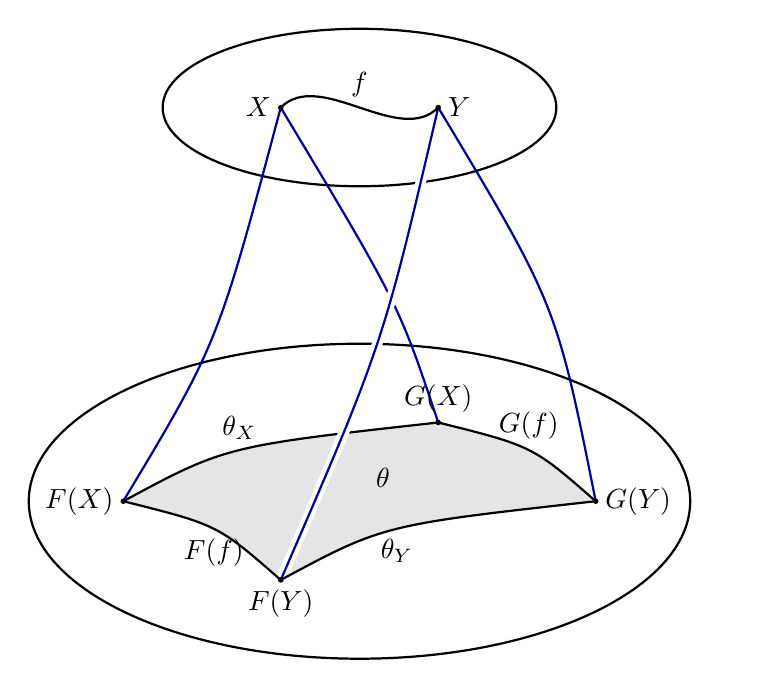
\begin{tikzpicture}
        \draw[thick] (0,3) ellipse (2.5 and 1)
        (0,-2) ellipse (4.2 and 2)
        node at (3, 3) {$\cC$}
        node at (4.7, -2) {$\cD$}
        coordinate (X) at (-1, 3)
        coordinate (Y) at (1, 3)
        coordinate (FX) at (-3, -2)
        coordinate (GY) at (3, -2)
        coordinate (GX) at (1, -1)
        coordinate (FY) at (-1, -3)
        coordinate (FX-GX-ct1) at (-1.7, -1.3)
        coordinate (FY-GY-ct1) at (0.3, -2.3)
        coordinate (FX-FY-ct1) at (-1.8, -2.3)
        coordinate (GX-GY-ct1) at (2.2, -1.3)
        coordinate (X-FX-ct1) at (-1.8, 0)
        coordinate (Y-FY-ct1) at (0.3, 0)
        coordinate (X-GX-ct1) at (0.5, 0.5)
        coordinate (Y-GY-ct1) at (2.5, 0.5);

        \fill[gray!20] (FX) .. controls (FX-GX-ct1) .. (GX) .. controls (GX-GY-ct1) .. (GY) .. controls (FY-GY-ct1) .. (FY) .. controls (FX-FY-ct1) .. (FX) -- cycle;

        \node at (0.3, -1.7) {$\theta$};

        \draw[thick] (FX) .. controls (FX-GX-ct1) .. node[above] {$\theta_X$} (GX) .. controls (GX-GY-ct1) .. node[above] {$G(f)$} (GY);
        \draw[thick,draw=blue!60!black] (X) .. controls (X-FX-ct1) .. (FX) (X) .. controls (X-GX-ct1) .. (GX);
        \draw[draw=white,double=blue!60!black,line width=1.5pt,double distance=0.8pt] (Y) .. controls (Y-FY-ct1) .. (FY);
        \draw[thick,draw=blue!60!black] (Y) .. controls (Y-GY-ct1) .. (GY);
        \draw[thick] (FX) .. controls (FX-FY-ct1) .. node[below] {$F(f)$} (FY) .. controls (FY-GY-ct1) .. node[below] {$\theta_Y$} (GY);
        \draw[thick] (X) .. controls (-.5, 3.5) and (.5, 2.5) .. node[above] {$f$} (Y);

        \node[left] at (X) {$X$};
        \node[right] at (Y) {$Y$};
        \node[left] at (FX) {$F(X)$};
        \node[right] at (GY) {$G(Y)$};
        \node[above] at (GX) {$G(X)$};
        \node[below] at (FY) {$F(Y)$};

        \foreach \point in {X, Y, FX, GX, GY, FY}
        \fill[black] (\point) circle (1pt);
    \end{tikzpicture}
    \caption{自然变换的几何直观}
    \label{fig:natural-transformation}
\end{figure}

首先,我们在一张纸上画两个面,表示两个范畴$\cC,\cD$. 在一个面上取两个点 $X, Y$,这是它上面的两个对象;然后,在另一个面上取四个点,分别表示 $F(X), F(Y), G(X), G(Y)$,即两个函子$F,G$在这两个点$X,Y$的取值. 注意,实际上两个函子分别是两个面之间的映射,如果把原像和像用线连接,展开来看的话,大概能看成是纸面上和纸面下的两张带有纹路的曲面. 然后,自然变换就是这两个曲面之间的连线$\theta$,对应到交换图上来,就是图中阴影区域的四条边. 实际上,我们的条件就是要求,这两族曲面$F, G$的结构和曲面之间的结构$\theta$都具备合适的连续性,如\autoref{fig:natural-transformation},这个东西在拓扑学中一般称为\term{同伦}.

在实践中,我们一般会称态射 $\theta_X$ 对于 $X$ 来说是自然的、典范的,或者说它满足函子性. 我们来看两个例子:

\begin{example}{}{}
    一个线性空间到某个商空间的投影映射. 考虑所有包含子空间 $U$ 的有限维线性空间. 显然,它们构成一个范畴,其间的态射定义为限制在 $U$ 上为恒同映射的线性映射,我们将这个东西记作 $\FVect_\F^U$.

    实际上,我们在说的是,考虑一个函子 $p\colon \FVect_\F^U \to \FVect_\F$ 将线性空间 $X$ 映到线性空间 $X/U$,另一个函子 $i\colon \FVect_\F^U \to \FVect_\F$ 将线性空间 $X$ 映到线性空间 $X$ 自身. 态射的映射都是显然的. 接下来,我们要表明存在一个自然变换 $\theta: i \to p$.

    现在,取任意的 $f\colon X \to Y$ 为 $\FVect_\F^U$ 中的态射,则我们需要使其交换的图表如下:

    \begin{center}
        \begin{tikzcd}
            X \rar["\theta_X"] \dar["f", swap] & X/U \dar["f/U"] \\
            Y \rar["\theta_Y", swap] & Y/U
        \end{tikzcd}
    \end{center}

    其中 $f/U$ 表示诱导的商映射,我们在不变子空间那一节中有所提及. 其中的 $\theta_X$ 和 $\theta_Y$ 就是我们通常称的典范投影,这也就是为什么这个投影被称为典范的.
\end{example}

下一个典范的结构我们也已经有所提及,它事关双对偶空间. 为了方便起见,对于函子 $F: \cC \to \cD$,我们记 $F^\mathrm{op}: \cC^\mathrm{op} \to \cD^\mathrm{op}$,它和原来的函子其实毫无差别,只有一点形式上的不同. 记对偶函子为 $-^*$,这是因为我们通常用 $V^*$ 表示对偶的空间,$f^*$ 表示对偶映射. 那么,我们就有 $(-^*)^\mathrm{op} \circ -^*$ 是典范同构. 这个事情的证明也是检查交换图,我们早已构造了这样的映射,也就是所谓的到双对偶空间的典范同构.

最后一个例子稍微有点特别,为了给出这个例子,我们需要定义一个与自然变换稍微有点不同的东西,强名之曰自然反变换\footnote{英文为 dinatural transformation,这个翻译稍微有点奇怪,但凑合用. }. 它的目标实际上是处理一些反变函子的情形,其它定义完全一致,不过它要求:$F: \cC \to \cD, G: \cC \to \cD^\mathrm{op}$,而它对应的交换图是:

\begin{center}
    \begin{tikzcd}
        F(X) \rar["\theta_X"] \dar["F(f)", swap] & G(X)\\
        F(Y) \rar["\theta_Y", swap] & G(Y) \uar["G(f)", swap]
    \end{tikzcd}
\end{center}

那么正如读者所料,我们要给出的结果就是:

\begin{example}{}{}
    不存在从一个线性空间到其对偶空间的非零自然反变换.

    现在,我们需要考虑下面的交换图:

    \begin{center}
        \begin{tikzcd}
            X \rar["\theta_X"] \dar["f", swap] & X^*\\
            Y \rar["\theta_Y", swap] & Y^* \uar["f^*", swap]
        \end{tikzcd}
    \end{center}

    我们知道,不管 $X$ 怎么取,总能取到一个 $f$ 使得 $f$ 将 $X$ 中的所有元素映到 $Y$ 中的零元,而参照我们的定义,这时的 $f^*$ 取值只有 $X^*$ 中的零元,因此,$\theta_X$ 为了让这个图交换,只能让所有元素映到零元.
\end{example}

可见在选取了合适的形式化方法之后,这些看上去无从下手的概念的证明变得无比单纯. 这实际上在表明,从一个空间到它的对偶空间不存在典范的同构.

\section{范畴论的构造}

单单是范畴、函子和自然变换显然什么都不能给出. 现在,我们无非是形式化了一些原来就已经说出的东西,顶多是最后对自然性的表述稍稍有些新意. 范畴论最核心的点实际上在于,它告诉了你很多被定义的东西实际上有其他的定义方式,这就是我们在这一节会讨论的内容.

\subsection{单态射、满态射和同构}

当我们在描述映射的时候,我们通常会讨论它是单的,满的,还是同构. 正如前面矩阵空间中关于指数映射的讨论中所表明的那样,这个性质实际上是非常不平凡的. 因此,这些性质应当在范畴论中得到恰当的推广——但是,时刻记住,现在我们的对象不同于以往我们做操作的集合,虽然我们还是能够从中汲取灵感.

先考虑集合的情况. 单射在我们看来,是如果像相同则原像相同,也就是说,每个原像集中的元素都有不同的像. 那么,就应当存在一个函数把它翻译回去,使得它在原像集上是恒同映射,也就是说:

\begin{lemma}{}{}
    考虑集合 $S, T$,一个函数 $f\colon T \to S$ 是单射当且仅当存在映射 $g\colon S \to T$ 使得 $g \circ f = \id_T$.
\end{lemma}

证明如上所述,形式化的写法留给读者,对偶地,我们就有:

\begin{lemma}{}{}
    $f\colon T \to S$ 是满射当且仅当存在映射 $g\colon S \to T$ 使得 $f \circ g = \id_S$.
\end{lemma}

而后面的这个定义是纯粹用箭头完成的,因此,它就能被推广到态射的情形:

\begin{definition}{}{}
    考虑范畴 $\cC$ 和其中的态射 $f\colon A \to B$.
    \begin{itemize}
        \item 称 $f$ 是\term{单态射},如果存在 $g\colon B \to A$ 使得 $g \circ f = \id_B$;
        \item 称 $f$ 是\term{满态射},如果存在 $g\colon B \to A$ 使得 $f \circ g = \id_A$;
        \item 称 $f$ 为\term{同构},如果存在 $g\colon B \to A$ 使得 $f \circ g = \id_A$ 且 $g \circ f = \id_B$;
        \item 如果 $A$ 和 $B$ 之间存在一个同构,则称 $A$ 和 $B$ 同构.
    \end{itemize}
\end{definition}

读者不难发现,恒同映射是一个同构. 这样的结构看上去就像一个逆元. 如果所有的态射都是同构,那么如果所有对象构成集合,态射也构成集合(这是为了避免一些集合论纷争),则我们将这个范畴构成一个\term{群胚}或者\term{广群}. 其态射集满足某种意义上的群结构. 实际上,在习题中我们会更进一步地发现相关的性质.

这里有一个麻烦的事情:同构一定既是单态射又是满态射,但既是单态射又是满态射的态射不一定是同构. 如果后者成立,则我们将这个范畴称为平衡范畴. 实际上,在通常的情形下,这个性质都是成立的.

\subsection{泛性质:始对象和终对象}

我们知道,一个范畴就是对象和箭头,那么,下面的定义看起来就很合乎情理:我们要选出箭头比较特殊的那些对象.

\begin{definition}{}{}
    称一个对象 $A \in \cC$ 为始对象,如果对于任意 $B \in \cC$ 都有 $|\Hom_\cC (A, B)| = 1$. 终对象是对偶范畴中的始对象. 如果一个对象既是始对象又是终对象,我们称其为零对象.
\end{definition}

注意,终对象的定义和始对象是完全对偶的,所以,很多时候我们其实不太区分这两种对象,它们具备的 $|\Hom_\cC (A, B)| = 1$ 的性质我们往往称为泛性质. 一般的,泛性质成立表明它实际上是一个定义性的东西:

\begin{theorem}{}{}
    所有始对象都是同构的、所有终对象都是同构的.
\end{theorem}

证明过于显然,留作读者练习. 重要的是例子:$\FVect$ 中,$\{1\}$ 是零对象. 这实际上说明了这个玩意的特殊性,但我们对它的特殊性早已习以为常. 剩下的一些例子我们会在后面的构造中一一给出——实际上,所有不太平凡的例子都要求我们构造一些更为奇特的范畴.

\subsection{Hom 函子和 Yoneda 引理}

注意到,如果 $\cC$ 和 $\cD$ 都是范畴,则 $\cC \times \cD$ 也是一个范畴,其上的对象和态射都是显然的. 我们首先考虑这样一个函子:
\[
    \Hom: \cC^\mathrm{op} \times \cC \to \Set
\]

它将对象 $(c, c')$ 映到它们之间的态射集 $\Hom_\cC(c, c')$,而将态射 $(f: c \leftarrow d, f': c' \to d')$ 映到一个 $\Hom_\cC(c, c') \to \Hom_\cC(d, d')$ 的映射,以复合的形式:
\[
    \Hom(f, f')(q: c \to c') = f' \circ q \circ f
\]

这个东西看起来乌七八糟的,但是在后面谈到张量积的时候,这个定义会体现出一个非常明显的性质. 在此,我们考虑另一种

\subsection{伴随函子}

\subsection{逗号范畴}

\subsection{和与积、极限和余极限}

\subsection{纤维化和余纤维化}

\section{幺半范畴及其性质}

\subsection{函子范畴和单子}

\subsection{Beck 单子化定理*}

\subsection{张量积}

\section{2-范畴一瞥}

\subsection{伴随和伴随}

\subsection{作为 2-极限的逗号范畴}

\subsection{走向无穷范畴:为什么我们需要套娃?}

\begin{exercise}
    \exquote[——《收获与播种》,格罗滕迪克]{每一门科学,当我们不是将它作为能力和统治力的工具,而是作为我们人类世代以来努力追求的对知识的冒险历程,不是别的,就是这样一种和谐,从一个时期到另一个时期,或多或少,巨大而又丰富:在不同的时代和世纪中,对于依次出现的不同的主题,它展现给我们微妙而精细的对应,仿佛来自虚空。}

    \begin{enumerate}  % 若不需要编号,则直接使用 enumerate 环境
        \item 证明以下两个态射的性质:
        \begin{enumerate}
            \item 如果 $A$ 与 $B$ 同构,那么 $A$ 与 $B$ 之间的同构映射是唯一的;
            \item 函子保持态射的单、满性质.
        \end{enumerate}
    \end{enumerate}
\end{exercise}


\LUgroupsancheck

\makeatletter
\let\chapter\@std@chapter
\let\@std@chapter\relax
\makeatother

\backmatter
{\small
\printindex
\printindex[sym]
}

\end{document}
